%\documentclass[12pt,a4paper]{article}
\documentclass[12pt]{ociamthesis}
%\documentclass[12pt,twoside,a4paper]{thesis}

% Variables that controls behaviour
\usepackage{ifthen} % for conditional statements
\newboolean{pdflatex}
\setboolean{pdflatex}{false} % False for eps figures 

\newboolean{articletitles}
\setboolean{articletitles}{true} % False removes titles in references

\newboolean{uprightparticles}
\setboolean{uprightparticles}{false} %True for upright particle symbols

\newboolean{inbibliography}
\setboolean{inbibliography}{false} %True once you enter the bibliography

%% Can add some more lines from main-prl.tex to remove some sections
\newboolean{wordcount}
\setboolean{wordcount}{false} % False for normal usage; true for wordcount.sh


\usepackage{cite}
\usepackage{mciteplus}

% Get hyperlinks to captions and in references.
% These do not work with revtex. Use "hypertext" as class option instead.
\usepackage{hyperref}    % Hyperlinks in references
\usepackage[all]{hypcap} % Internal hyperlinks to floats.

%% Thing for fancyfoot
\usepackage{fancyhdr}

%% Thing for mini table of contents
\usepackage{minitoc}


%%% $Id: lhcb-symbols-def.tex 104802 2017-03-01 11:11:43Z thadaviz $
%%% ======================================================================
%%% Purpose: Standard LHCb aliases
%%% Author: Originally Ulrik Egede, adapted by Tomasz Skwarnicki for templates,
%%% rewritten by Chris Parkes
%%% Maintainer : Ulrik Egede (2010 - 2012)
%%% Maintainer : Rolf Oldeman (2012 - 2014)
%%% =======================================================================

%%% To use this file outside the normal LHCb document environment, the
%%% following should be added in a preamble (before \begin{document}
%%%
%%%\usepackage{ifthen} 
%%%\newboolean{uprightparticles}
%%%\setboolean{uprightparticles}{false} %Set true for upright particle symbols
\usepackage{xspace} 
\usepackage{upgreek}

%%%%%%%%%%%%%%%%%%%%%%%%%%%%%%%%%%%%%%%%%%%%%%%%%%%%%%%%%%%%
%%%
%%% The following is to ensure that the template automatically can process
%%% this file.
%%%
%%% Add comments with at least three %%% preceding.
%%% Add new sections with one % preceding
%%% Add new subsections with two %% preceding
%%%%%%%%%%%%%%%%%%%%%%%%%%%%%%%%%%%%%%%%%%%%%%%%%%%%%%%%%%%%

%%%%%%%%%%%%%
% Experiments
%%%%%%%%%%%%%
\def\lhcb {\mbox{LHCb}\xspace}
\def\atlas  {\mbox{ATLAS}\xspace}
\def\cms    {\mbox{CMS}\xspace}
\def\alice  {\mbox{ALICE}\xspace}
\def\babar  {\mbox{BaBar}\xspace}
\def\belle  {\mbox{Belle}\xspace}
\def\cleo   {\mbox{CLEO}\xspace}
\def\cdf    {\mbox{CDF}\xspace}
\def\dzero  {\mbox{D0}\xspace}
\def\aleph  {\mbox{ALEPH}\xspace}
\def\delphi {\mbox{DELPHI}\xspace}
\def\opal   {\mbox{OPAL}\xspace}
\def\lthree {\mbox{L3}\xspace}
\def\sld    {\mbox{SLD}\xspace}
%%%\def\argus  {\mbox{ARGUS}\xspace}
%%%\def\uaone  {\mbox{UA1}\xspace}
%%%\def\uatwo  {\mbox{UA2}\xspace}
%%%\def\ux85 {\mbox{UX85}\xspace}
\def\cern {\mbox{CERN}\xspace}
\def\lhc    {\mbox{LHC}\xspace}
\def\lep    {\mbox{LEP}\xspace}
\def\tevatron {Tevatron\xspace}

%% LHCb sub-detectors and sub-systems

%%%\def\pu     {PU\xspace}
\def\velo   {VELO\xspace}
\def\rich   {RICH\xspace}
\def\richone {RICH1\xspace}
\def\richtwo {RICH2\xspace}
\def\ttracker {TT\xspace}
\def\intr   {IT\xspace}
\def\st     {ST\xspace}
\def\ot     {OT\xspace}
\def\herschel {\mbox{\textsc{HeRSCheL}}\xspace}
%%%\def\Tone   {T1\xspace}
%%%\def\Ttwo   {T2\xspace}
%%%\def\Tthree {T3\xspace}
%%%\def\Mone   {M1\xspace}
%%%\def\Mtwo   {M2\xspace}
%%%\def\Mthree {M3\xspace}
%%%\def\Mfour  {M4\xspace}
%%%\def\Mfive  {M5\xspace}
\def\spd    {SPD\xspace}
\def\presh  {PS\xspace}
\def\ecal   {ECAL\xspace}
\def\hcal   {HCAL\xspace}
%%%\def\bcm    {BCM\xspace}
\def\MagUp {\mbox{\em Mag\kern -0.05em Up}\xspace}
\def\MagDown {\mbox{\em MagDown}\xspace}

\def\ode    {ODE\xspace}
\def\daq    {DAQ\xspace}
\def\tfc    {TFC\xspace}
\def\ecs    {ECS\xspace}
\def\lone   {L0\xspace}
\def\hlt    {HLT\xspace}
\def\hltone {HLT1\xspace}
\def\hlttwo {HLT2\xspace}

%%% Upright (not slanted) Particles

\ifthenelse{\boolean{uprightparticles}}%
{\def\Palpha      {\ensuremath{\upalpha}\xspace}
 \def\Pbeta       {\ensuremath{\upbeta}\xspace}
 \def\Pgamma      {\ensuremath{\upgamma}\xspace}                 
 \def\Pdelta      {\ensuremath{\updelta}\xspace}                 
 \def\Pepsilon    {\ensuremath{\upepsilon}\xspace}                 
 \def\Pvarepsilon {\ensuremath{\upvarepsilon}\xspace}                 
 \def\Pzeta       {\ensuremath{\upzeta}\xspace}                 
 \def\Peta        {\ensuremath{\upeta}\xspace}                 
 \def\Ptheta      {\ensuremath{\uptheta}\xspace}                 
 \def\Pvartheta   {\ensuremath{\upvartheta}\xspace}                 
 \def\Piota       {\ensuremath{\upiota}\xspace}                 
 \def\Pkappa      {\ensuremath{\upkappa}\xspace}                 
 \def\Plambda     {\ensuremath{\uplambda}\xspace}                 
 \def\Pmu         {\ensuremath{\upmu}\xspace}                 
 \def\Pnu         {\ensuremath{\upnu}\xspace}                 
 \def\Pxi         {\ensuremath{\upxi}\xspace}                 
 \def\Ppi         {\ensuremath{\uppi}\xspace}                 
 \def\Pvarpi      {\ensuremath{\upvarpi}\xspace}                 
 \def\Prho        {\ensuremath{\uprho}\xspace}                 
 \def\Pvarrho     {\ensuremath{\upvarrho}\xspace}                 
 \def\Ptau        {\ensuremath{\uptau}\xspace}                 
 \def\Pupsilon    {\ensuremath{\upupsilon}\xspace}                 
 \def\Pphi        {\ensuremath{\upphi}\xspace}                 
 \def\Pvarphi     {\ensuremath{\upvarphi}\xspace}                 
 \def\Pchi        {\ensuremath{\upchi}\xspace}                 
 \def\Ppsi        {\ensuremath{\uppsi}\xspace}                 
 \def\Pomega      {\ensuremath{\upomega}\xspace}                 

 \def\PDelta      {\ensuremath{\Delta}\xspace}                 
 \def\PXi      {\ensuremath{\Xi}\xspace}                 
 \def\PLambda      {\ensuremath{\Lambda}\xspace}                 
 \def\PSigma      {\ensuremath{\Sigma}\xspace}                 
 \def\POmega      {\ensuremath{\Omega}\xspace}                 
 \def\PUpsilon      {\ensuremath{\Upsilon}\xspace}                 
 
 %\mathchardef\Deltares="7101
 %\mathchardef\Xi="7104
 %\mathchardef\Lambda="7103
 %\mathchardef\Sigma="7106
 %\mathchardef\Omega="710A


 \def\PA      {\ensuremath{\mathrm{A}}\xspace}                 
 \def\PB      {\ensuremath{\mathrm{B}}\xspace}                 
 \def\PC      {\ensuremath{\mathrm{C}}\xspace}                 
 \def\PD      {\ensuremath{\mathrm{D}}\xspace}                 
 \def\PE      {\ensuremath{\mathrm{E}}\xspace}                 
 \def\PF      {\ensuremath{\mathrm{F}}\xspace}                 
 \def\PG      {\ensuremath{\mathrm{G}}\xspace}                 
 \def\PH      {\ensuremath{\mathrm{H}}\xspace}                 
 \def\PI      {\ensuremath{\mathrm{I}}\xspace}                 
 \def\PJ      {\ensuremath{\mathrm{J}}\xspace}                 
 \def\PK      {\ensuremath{\mathrm{K}}\xspace}                 
 \def\PL      {\ensuremath{\mathrm{L}}\xspace}                 
 \def\PM      {\ensuremath{\mathrm{M}}\xspace}                 
 \def\PN      {\ensuremath{\mathrm{N}}\xspace}                 
 \def\PO      {\ensuremath{\mathrm{O}}\xspace}                 
 \def\PP      {\ensuremath{\mathrm{P}}\xspace}                 
 \def\PQ      {\ensuremath{\mathrm{Q}}\xspace}                 
 \def\PR      {\ensuremath{\mathrm{R}}\xspace}                 
 \def\PS      {\ensuremath{\mathrm{S}}\xspace}                 
 \def\PT      {\ensuremath{\mathrm{T}}\xspace}                 
 \def\PU      {\ensuremath{\mathrm{U}}\xspace}                 
 \def\PV      {\ensuremath{\mathrm{V}}\xspace}                 
 \def\PW      {\ensuremath{\mathrm{W}}\xspace}                 
 \def\PX      {\ensuremath{\mathrm{X}}\xspace}                 
 \def\PY      {\ensuremath{\mathrm{Y}}\xspace}                 
 \def\PZ      {\ensuremath{\mathrm{Z}}\xspace}                 
 \def\Pa      {\ensuremath{\mathrm{a}}\xspace}                 
 \def\Pb      {\ensuremath{\mathrm{b}}\xspace}                 
 \def\Pc      {\ensuremath{\mathrm{c}}\xspace}                 
 \def\Pd      {\ensuremath{\mathrm{d}}\xspace}                 
 \def\Pe      {\ensuremath{\mathrm{e}}\xspace}                 
 \def\Pf      {\ensuremath{\mathrm{f}}\xspace}                 
 \def\Pg      {\ensuremath{\mathrm{g}}\xspace}                 
 \def\Ph      {\ensuremath{\mathrm{h}}\xspace}                 
 \def\Pi      {\ensuremath{\mathrm{i}}\xspace}                 
 \def\Pj      {\ensuremath{\mathrm{j}}\xspace}                 
 \def\Pk      {\ensuremath{\mathrm{k}}\xspace}                 
 \def\Pl      {\ensuremath{\mathrm{l}}\xspace}                 
 \def\Pm      {\ensuremath{\mathrm{m}}\xspace}                 
 \def\Pn      {\ensuremath{\mathrm{n}}\xspace}                 
 \def\Po      {\ensuremath{\mathrm{o}}\xspace}                 
 \def\Pp      {\ensuremath{\mathrm{p}}\xspace}                 
 \def\Pq      {\ensuremath{\mathrm{q}}\xspace}                 
 \def\Pr      {\ensuremath{\mathrm{r}}\xspace}                 
 \def\Ps      {\ensuremath{\mathrm{s}}\xspace}                 
 \def\Pt      {\ensuremath{\mathrm{t}}\xspace}                 
 \def\Pu      {\ensuremath{\mathrm{u}}\xspace}                 
 \def\Pv      {\ensuremath{\mathrm{v}}\xspace}                 
 \def\Pw      {\ensuremath{\mathrm{w}}\xspace}                 
 \def\Px      {\ensuremath{\mathrm{x}}\xspace}                 
 \def\Py      {\ensuremath{\mathrm{y}}\xspace}                 
 \def\Pz      {\ensuremath{\mathrm{z}}\xspace}                 
}
{\def\Palpha      {\ensuremath{\alpha}\xspace}
 \def\Pbeta       {\ensuremath{\beta}\xspace}
 \def\Pgamma      {\ensuremath{\gamma}\xspace}                 
 \def\Pdelta      {\ensuremath{\delta}\xspace}                 
 \def\Pepsilon    {\ensuremath{\epsilon}\xspace}                 
 \def\Pvarepsilon {\ensuremath{\varepsilon}\xspace}                 
 \def\Pzeta       {\ensuremath{\zeta}\xspace}                 
 \def\Peta        {\ensuremath{\eta}\xspace}                 
 \def\Ptheta      {\ensuremath{\theta}\xspace}                 
 \def\Pvartheta   {\ensuremath{\vartheta}\xspace}                 
 \def\Piota       {\ensuremath{\iota}\xspace}                 
 \def\Pkappa      {\ensuremath{\kappa}\xspace}                 
 \def\Plambda     {\ensuremath{\lambda}\xspace}                 
 \def\Pmu         {\ensuremath{\mu}\xspace}                 
 \def\Pnu         {\ensuremath{\nu}\xspace}                 
 \def\Pxi         {\ensuremath{\xi}\xspace}                 
 \def\Ppi         {\ensuremath{\pi}\xspace}                 
 \def\Pvarpi      {\ensuremath{\varpi}\xspace}                 
 \def\Prho        {\ensuremath{\rho}\xspace}                 
 \def\Pvarrho     {\ensuremath{\varrho}\xspace}                 
 \def\Ptau        {\ensuremath{\tau}\xspace}                 
 \def\Pupsilon    {\ensuremath{\upsilon}\xspace}                 
 \def\Pphi        {\ensuremath{\phi}\xspace}                 
 \def\Pvarphi     {\ensuremath{\varphi}\xspace}                 
 \def\Pchi        {\ensuremath{\chi}\xspace}                 
 \def\Ppsi        {\ensuremath{\psi}\xspace}                 
 \def\Pomega      {\ensuremath{\omega}\xspace}                 
 \mathchardef\PDelta="7101
 \mathchardef\PXi="7104
 \mathchardef\PLambda="7103
 \mathchardef\PSigma="7106
 \mathchardef\POmega="710A
 \mathchardef\PUpsilon="7107
 \def\PA      {\ensuremath{A}\xspace}                 
 \def\PB      {\ensuremath{B}\xspace}                 
 \def\PC      {\ensuremath{C}\xspace}                 
 \def\PD      {\ensuremath{D}\xspace}                 
 \def\PE      {\ensuremath{E}\xspace}                 
 \def\PF      {\ensuremath{F}\xspace}                 
 \def\PG      {\ensuremath{G}\xspace}                 
 \def\PH      {\ensuremath{H}\xspace}                 
 \def\PI      {\ensuremath{I}\xspace}                 
 \def\PJ      {\ensuremath{J}\xspace}                 
 \def\PK      {\ensuremath{K}\xspace}                 
 \def\PL      {\ensuremath{L}\xspace}                 
 \def\PM      {\ensuremath{M}\xspace}                 
 \def\PN      {\ensuremath{N}\xspace}                 
 \def\PO      {\ensuremath{O}\xspace}                 
 \def\PP      {\ensuremath{P}\xspace}                 
 \def\PQ      {\ensuremath{Q}\xspace}                 
 \def\PR      {\ensuremath{R}\xspace}                 
 \def\PS      {\ensuremath{S}\xspace}                 
 \def\PT      {\ensuremath{T}\xspace}                 
 \def\PU      {\ensuremath{U}\xspace}                 
 \def\PV      {\ensuremath{V}\xspace}                 
 \def\PW      {\ensuremath{W}\xspace}                 
 \def\PX      {\ensuremath{X}\xspace}                 
 \def\PY      {\ensuremath{Y}\xspace}                 
 \def\PZ      {\ensuremath{Z}\xspace}                 
 \def\Pa      {\ensuremath{a}\xspace}                 
 \def\Pb      {\ensuremath{b}\xspace}                 
 \def\Pc      {\ensuremath{c}\xspace}                 
 \def\Pd      {\ensuremath{d}\xspace}                 
 \def\Pe      {\ensuremath{e}\xspace}                 
 \def\Pf      {\ensuremath{f}\xspace}                 
 \def\Pg      {\ensuremath{g}\xspace}                 
 \def\Ph      {\ensuremath{h}\xspace}                 
 \def\Pi      {\ensuremath{i}\xspace}                 
 \def\Pj      {\ensuremath{j}\xspace}                 
 \def\Pk      {\ensuremath{k}\xspace}                 
 \def\Pl      {\ensuremath{l}\xspace}                 
 \def\Pm      {\ensuremath{m}\xspace}                 
 \def\Pn      {\ensuremath{n}\xspace}                 
 \def\Po      {\ensuremath{o}\xspace}                 
 \def\Pp      {\ensuremath{p}\xspace}                 
 \def\Pq      {\ensuremath{q}\xspace}                 
 \def\Pr      {\ensuremath{r}\xspace}                 
 \def\Ps      {\ensuremath{s}\xspace}                 
 \def\Pt      {\ensuremath{t}\xspace}                 
 \def\Pu      {\ensuremath{u}\xspace}                 
 \def\Pv      {\ensuremath{v}\xspace}                 
 \def\Pw      {\ensuremath{w}\xspace}                 
 \def\Px      {\ensuremath{x}\xspace}                 
 \def\Py      {\ensuremath{y}\xspace}                 
 \def\Pz      {\ensuremath{z}\xspace}                 
}

%%%%%%%%%%%%%%%%%%%%%%%%%%%%%%%%%%%%%%%%%%%%%%%
% Particles
\makeatletter
\ifcase \@ptsize \relax% 10pt
  \newcommand{\miniscule}{\@setfontsize\miniscule{4}{5}}% \tiny: 5/6
\or% 11pt
  \newcommand{\miniscule}{\@setfontsize\miniscule{5}{6}}% \tiny: 6/7
\or% 12pt
  \newcommand{\miniscule}{\@setfontsize\miniscule{5}{6}}% \tiny: 6/7
\fi
\makeatother


\DeclareRobustCommand{\optbar}[1]{\shortstack{{\miniscule (\rule[.5ex]{1.25em}{.18mm})}
  \\ [-.7ex] $#1$}}


%% Leptons

\let\emi\en
\def\electron   {{\ensuremath{\Pe}}\xspace}
\def\en         {{\ensuremath{\Pe^-}}\xspace}   % electron negative (\em is taken)
\def\ep         {{\ensuremath{\Pe^+}}\xspace}
\def\epm        {{\ensuremath{\Pe^\pm}}\xspace} 
\def\epem       {{\ensuremath{\Pe^+\Pe^-}}\xspace}
%%%\def\ee         {\ensuremath{\Pe^-\Pe^-}\xspace}

\def\muon       {{\ensuremath{\Pmu}}\xspace}
\def\mup        {{\ensuremath{\Pmu^+}}\xspace}
\def\mun        {{\ensuremath{\Pmu^-}}\xspace} % muon negative (\mum is taken)
\def\mumu       {{\ensuremath{\Pmu^+\Pmu^-}}\xspace}

\def\tauon      {{\ensuremath{\Ptau}}\xspace}
\def\taup       {{\ensuremath{\Ptau^+}}\xspace}
\def\taum       {{\ensuremath{\Ptau^-}}\xspace}
\def\tautau     {{\ensuremath{\Ptau^+\Ptau^-}}\xspace}

\def\lepton     {{\ensuremath{\ell}}\xspace}
\def\ellm       {{\ensuremath{\ell^-}}\xspace}
\def\ellp       {{\ensuremath{\ell^+}}\xspace}
\def\ellell     {\ensuremath{\ell^+ \ell^-}\xspace}

\def\neu        {{\ensuremath{\Pnu}}\xspace}
\def\neub       {{\ensuremath{\overline{\Pnu}}}\xspace}
%%%\def\nuenueb    {\ensuremath{\neu\neub}\xspace}
\def\neue       {{\ensuremath{\neu_e}}\xspace}
\def\neueb      {{\ensuremath{\neub_e}}\xspace}
%%%\def\neueneueb  {\ensuremath{\neue\neueb}\xspace}
\def\neum       {{\ensuremath{\neu_\mu}}\xspace}
\def\neumb      {{\ensuremath{\neub_\mu}}\xspace}
%%%\def\neumneumb  {\ensuremath{\neum\neumb}\xspace}
\def\neut       {{\ensuremath{\neu_\tau}}\xspace}
\def\neutb      {{\ensuremath{\neub_\tau}}\xspace}
%%%\def\neutneutb  {\ensuremath{\neut\neutb}\xspace}
\def\neul       {{\ensuremath{\neu_\ell}}\xspace}
\def\neulb      {{\ensuremath{\neub_\ell}}\xspace}
%%%\def\neulneulb  {\ensuremath{\neul\neulb}\xspace}

%% Gauge bosons and scalars

\def\g      {{\ensuremath{\Pgamma}}\xspace}
\def\H      {{\ensuremath{\PH^0}}\xspace}
\def\Hp     {{\ensuremath{\PH^+}}\xspace}
\def\Hm     {{\ensuremath{\PH^-}}\xspace}
\def\Hpm    {{\ensuremath{\PH^\pm}}\xspace}
\def\W      {{\ensuremath{\PW}}\xspace}
\def\Wp     {{\ensuremath{\PW^+}}\xspace}
\def\Wm     {{\ensuremath{\PW^-}}\xspace}
\def\Wpm    {{\ensuremath{\PW^\pm}}\xspace}
\def\Z      {{\ensuremath{\PZ}}\xspace}

%% Quarks

\def\quark     {{\ensuremath{\Pq}}\xspace}
\def\quarkbar  {{\ensuremath{\overline \quark}}\xspace}
\def\qqbar     {{\ensuremath{\quark\quarkbar}}\xspace}
\def\uquark    {{\ensuremath{\Pu}}\xspace}
\def\uquarkbar {{\ensuremath{\overline \uquark}}\xspace}
\def\uubar     {{\ensuremath{\uquark\uquarkbar}}\xspace}
\def\dquark    {{\ensuremath{\Pd}}\xspace}
\def\dquarkbar {{\ensuremath{\overline \dquark}}\xspace}
\def\ddbar     {{\ensuremath{\dquark\dquarkbar}}\xspace}
\def\squark    {{\ensuremath{\Ps}}\xspace}
\def\squarkbar {{\ensuremath{\overline \squark}}\xspace}
\def\ssbar     {{\ensuremath{\squark\squarkbar}}\xspace}
\def\cquark    {{\ensuremath{\Pc}}\xspace}
\def\cquarkbar {{\ensuremath{\overline \cquark}}\xspace}
\def\ccbar     {{\ensuremath{\cquark\cquarkbar}}\xspace}
\def\bquark    {{\ensuremath{\Pb}}\xspace}
\def\bquarkbar {{\ensuremath{\overline \bquark}}\xspace}
\def\bbbar     {{\ensuremath{\bquark\bquarkbar}}\xspace}
\def\tquark    {{\ensuremath{\Pt}}\xspace}
\def\tquarkbar {{\ensuremath{\overline \tquark}}\xspace}
\def\ttbar     {{\ensuremath{\tquark\tquarkbar}}\xspace}

%% Light mesons

\def\hadron {{\ensuremath{\Ph}}\xspace}
\def\pion   {{\ensuremath{\Ppi}}\xspace}
\def\piz    {{\ensuremath{\pion^0}}\xspace}
\def\pizs   {{\ensuremath{\pion^0\mbox\,\mathrm{s}}}\xspace}
\def\pip    {{\ensuremath{\pion^+}}\xspace}
\def\pim    {{\ensuremath{\pion^-}}\xspace}
\def\pipm   {{\ensuremath{\pion^\pm}}\xspace}
\def\pimp   {{\ensuremath{\pion^\mp}}\xspace}

\def\rhomeson {{\ensuremath{\Prho}}\xspace}
\def\rhoz     {{\ensuremath{\rhomeson^0}}\xspace}
\def\rhop     {{\ensuremath{\rhomeson^+}}\xspace}
\def\rhom     {{\ensuremath{\rhomeson^-}}\xspace}
\def\rhopm    {{\ensuremath{\rhomeson^\pm}}\xspace}
\def\rhomp    {{\ensuremath{\rhomeson^\mp}}\xspace}

\def\kaon    {{\ensuremath{\PK}}\xspace}
%%% do NOT use ensuremath here
  \def\Kbar    {{\kern 0.2em\overline{\kern -0.2em \PK}{}}\xspace}
\def\Kb      {{\ensuremath{\Kbar}}\xspace}
\def\KorKbar    {\kern 0.18em\optbar{\kern -0.18em K}{}\xspace}
\def\Kz      {{\ensuremath{\kaon^0}}\xspace}
\def\Kzb     {{\ensuremath{\Kbar{}^0}}\xspace}
\def\Kp      {{\ensuremath{\kaon^+}}\xspace}
\def\Km      {{\ensuremath{\kaon^-}}\xspace}
\def\Kpm     {{\ensuremath{\kaon^\pm}}\xspace}
\def\Kmp     {{\ensuremath{\kaon^\mp}}\xspace}
\def\KS      {{\ensuremath{\kaon^0_{\mathrm{ \scriptscriptstyle S}}}}\xspace}
\def\KL      {{\ensuremath{\kaon^0_{\mathrm{ \scriptscriptstyle L}}}}\xspace}
\def\Kstarz  {{\ensuremath{\kaon^{*0}}}\xspace}
\def\Kstarzb {{\ensuremath{\Kbar{}^{*0}}}\xspace}
\def\Kstar   {{\ensuremath{\kaon^*}}\xspace}
\def\Kstarb  {{\ensuremath{\Kbar{}^*}}\xspace}
\def\Kstarp  {{\ensuremath{\kaon^{*+}}}\xspace}
\def\Kstarm  {{\ensuremath{\kaon^{*-}}}\xspace}
\def\Kstarpm {{\ensuremath{\kaon^{*\pm}}}\xspace}
\def\Kstarmp {{\ensuremath{\kaon^{*\mp}}}\xspace}

\newcommand{\etaz}{\ensuremath{\Peta}\xspace}
\newcommand{\etapr}{\ensuremath{\Peta^{\prime}}\xspace}
\newcommand{\phiz}{\ensuremath{\Pphi}\xspace}
\newcommand{\omegaz}{\ensuremath{\Pomega}\xspace}

%% Heavy mesons

%%% do NOT use ensuremath here
  \def\Dbar    {{\kern 0.2em\overline{\kern -0.2em \PD}{}}\xspace}
\def\D       {{\ensuremath{\PD}}\xspace}
\def\Db      {{\ensuremath{\Dbar}}\xspace}
\def\DorDbar    {\kern 0.18em\optbar{\kern -0.18em D}{}\xspace}
\def\Dz      {{\ensuremath{\D^0}}\xspace}
\def\Dzb     {{\ensuremath{\Dbar{}^0}}\xspace}
\def\Dp      {{\ensuremath{\D^+}}\xspace}
\def\Dm      {{\ensuremath{\D^-}}\xspace}
\def\Dpm     {{\ensuremath{\D^\pm}}\xspace}
\def\Dmp     {{\ensuremath{\D^\mp}}\xspace}
\def\Dstar   {{\ensuremath{\D^*}}\xspace}
\def\Dstarb  {{\ensuremath{\Dbar{}^*}}\xspace}
\def\Dstarz  {{\ensuremath{\D^{*0}}}\xspace}
\def\Dstarzb {{\ensuremath{\Dbar{}^{*0}}}\xspace}
\def\Dstarp  {{\ensuremath{\D^{*+}}}\xspace}
\def\Dstarm  {{\ensuremath{\D^{*-}}}\xspace}
\def\Dstarpm {{\ensuremath{\D^{*\pm}}}\xspace}
\def\Dstarmp {{\ensuremath{\D^{*\mp}}}\xspace}
\def\Ds      {{\ensuremath{\D_\squark}}\xspace}
\def\Dsp     {{\ensuremath{\D^+_\squark}}\xspace}
\def\Dsm     {{\ensuremath{\D^-_\squark}}\xspace}
\def\Dspm    {{\ensuremath{\D^{\pm}_\squark}}\xspace}
\def\Dsmp    {{\ensuremath{\D^{\mp}_\squark}}\xspace}
\def\Dss     {{\ensuremath{\D^{*+}_\squark}}\xspace}
\def\Dssp    {{\ensuremath{\D^{*+}_\squark}}\xspace}
\def\Dssm    {{\ensuremath{\D^{*-}_\squark}}\xspace}
\def\Dsspm   {{\ensuremath{\D^{*\pm}_\squark}}\xspace}
\def\Dssmp   {{\ensuremath{\D^{*\mp}_\squark}}\xspace}

\def\B       {{\ensuremath{\PB}}\xspace}
%%% do NOT use ensuremath here
\def\Bbar    {{\ensuremath{\kern 0.18em\overline{\kern -0.18em \PB}{}}}\xspace}
\def\Bb      {{\ensuremath{\Bbar}}\xspace}
\def\BorBbar    {\kern 0.18em\optbar{\kern -0.18em B}{}\xspace}
\def\Bz      {{\ensuremath{\B^0}}\xspace}
\def\Bzb     {{\ensuremath{\Bbar{}^0}}\xspace}
\def\Bu      {{\ensuremath{\B^+}}\xspace}
\def\Bub     {{\ensuremath{\B^-}}\xspace}
\def\Bp      {{\ensuremath{\Bu}}\xspace}
\def\Bm      {{\ensuremath{\Bub}}\xspace}
\def\Bpm     {{\ensuremath{\B^\pm}}\xspace}
\def\Bmp     {{\ensuremath{\B^\mp}}\xspace}
\def\Bd      {{\ensuremath{\B^0}}\xspace}
\def\Bs      {{\ensuremath{\B^0_\squark}}\xspace}
\def\Bsb     {{\ensuremath{\Bbar{}^0_\squark}}\xspace}
\def\Bdb     {{\ensuremath{\Bbar{}^0}}\xspace}
\def\Bc      {{\ensuremath{\B_\cquark^+}}\xspace}
\def\Bcp     {{\ensuremath{\B_\cquark^+}}\xspace}
\def\Bcm     {{\ensuremath{\B_\cquark^-}}\xspace}
\def\Bcpm    {{\ensuremath{\B_\cquark^\pm}}\xspace}

%% Onia

\def\jpsi     {{\ensuremath{{\PJ\mskip -3mu/\mskip -2mu\Ppsi\mskip 2mu}}}\xspace}
\def\psitwos  {{\ensuremath{\Ppsi{(2S)}}}\xspace}
\def\psiprpr  {{\ensuremath{\Ppsi(3770)}}\xspace}
\def\etac     {{\ensuremath{\Peta_\cquark}}\xspace}
\def\chiczero {{\ensuremath{\Pchi_{\cquark 0}}}\xspace}
\def\chicone  {{\ensuremath{\Pchi_{\cquark 1}}}\xspace}
\def\chictwo  {{\ensuremath{\Pchi_{\cquark 2}}}\xspace}
  %\mathchardef\Upsilon="7107
  \def\Y#1S{\ensuremath{\PUpsilon{(#1S)}}\xspace}% no space before {...}!
\def\OneS  {{\Y1S}}
\def\TwoS  {{\Y2S}}
\def\ThreeS{{\Y3S}}
\def\FourS {{\Y4S}}
\def\FiveS {{\Y5S}}

\def\chic  {{\ensuremath{\Pchi_{c}}}\xspace}

%% Baryons

\def\proton      {{\ensuremath{\Pp}}\xspace}
\def\antiproton  {{\ensuremath{\overline \proton}}\xspace}
\def\neutron     {{\ensuremath{\Pn}}\xspace}
\def\antineutron {{\ensuremath{\overline \neutron}}\xspace}
\def\Deltares    {{\ensuremath{\PDelta}}\xspace}
\def\Deltaresbar {{\ensuremath{\overline \Deltares}}\xspace}
\def\Xires       {{\ensuremath{\PXi}}\xspace}
\def\Xiresbar    {{\ensuremath{\overline \Xires}}\xspace}
\def\Lz          {{\ensuremath{\PLambda}}\xspace}
\def\Lbar        {{\ensuremath{\kern 0.1em\overline{\kern -0.1em\PLambda}}}\xspace}
\def\LorLbar    {\kern 0.18em\optbar{\kern -0.18em \PLambda}{}\xspace}
\def\Lambdares   {{\ensuremath{\PLambda}}\xspace}
\def\Lambdaresbar{{\ensuremath{\Lbar}}\xspace}
\def\Sigmares    {{\ensuremath{\PSigma}}\xspace}
\def\Sigmaresbar {{\ensuremath{\overline \Sigmares}}\xspace}
\def\Omegares    {{\ensuremath{\POmega}}\xspace}
\def\Omegaresbar {{\ensuremath{\overline \POmega}}\xspace}

%%% do NOT use ensuremath here
 % \def\Deltabar{\kern 0.25em\overline{\kern -0.25em \Deltares}{}\xspace}
 % \def\Sigbar{\kern 0.2em\overline{\kern -0.2em \Sigma}{}\xspace}
 % \def\Xibar{\kern 0.2em\overline{\kern -0.2em \Xi}{}\xspace}
 % \def\Obar{\kern 0.2em\overline{\kern -0.2em \Omega}{}\xspace}
 % \def\Nbar{\kern 0.2em\overline{\kern -0.2em N}{}\xspace}
 % \def\Xb{\kern 0.2em\overline{\kern -0.2em X}{}\xspace}

\def\Lb      {{\ensuremath{\Lz^0_\bquark}}\xspace}
\def\Lbbar   {{\ensuremath{\Lbar{}^0_\bquark}}\xspace}
\def\Lc      {{\ensuremath{\Lz^+_\cquark}}\xspace}
\def\Lcbar   {{\ensuremath{\Lbar{}^-_\cquark}}\xspace}
\def\Xib     {{\ensuremath{\Xires_\bquark}}\xspace}
\def\Xibz    {{\ensuremath{\Xires^0_\bquark}}\xspace}
\def\Xibm    {{\ensuremath{\Xires^-_\bquark}}\xspace}
\def\Xibbar  {{\ensuremath{\Xiresbar{}_\bquark}}\xspace}
\def\Xibbarz {{\ensuremath{\Xiresbar{}_\bquark^0}}\xspace}
\def\Xibbarp {{\ensuremath{\Xiresbar{}_\bquark^+}}\xspace}
\def\Xic     {{\ensuremath{\Xires_\cquark}}\xspace}
\def\Xicz    {{\ensuremath{\Xires^0_\cquark}}\xspace}
\def\Xicp    {{\ensuremath{\Xires^+_\cquark}}\xspace}
\def\Xicbar  {{\ensuremath{\Xiresbar{}_\cquark}}\xspace}
\def\Xicbarz {{\ensuremath{\Xiresbar{}_\cquark^0}}\xspace}
\def\Xicbarm {{\ensuremath{\Xiresbar{}_\cquark^-}}\xspace}
\def\Omegac    {{\ensuremath{\Omegares^0_\cquark}}\xspace}
\def\Omegacbar {{\ensuremath{\Omegaresbar{}_\cquark^0}}\xspace}
\def\Omegab    {{\ensuremath{\Omegares^-_\bquark}}\xspace}
\def\Omegabbar {{\ensuremath{\Omegaresbar{}_\bquark^+}}\xspace}

%%%%%%%%%%%%%%%%%%
% Physics symbols
%%%%%%%%%%%%%%%%%

%% Decays
\def\BF         {{\ensuremath{\mathcal{B}}}\xspace}
\def\BRvis      {{\ensuremath{\BR_{\mathrm{{vis}}}}}}
\def\BR         {\BF}
\newcommand{\decay}[2]{\ensuremath{#1\!\to #2}\xspace}         % {\Pa}{\Pb \Pc}
\def\ra                 {\ensuremath{\rightarrow}\xspace}
\def\to                 {\ensuremath{\rightarrow}\xspace}

%% Lifetimes
\newcommand{\tauBs}{{\ensuremath{\tau_{\Bs}}}\xspace}
\newcommand{\tauBd}{{\ensuremath{\tau_{\Bd}}}\xspace}
\newcommand{\tauBz}{{\ensuremath{\tau_{\Bz}}}\xspace}
\newcommand{\tauBu}{{\ensuremath{\tau_{\Bp}}}\xspace}
\newcommand{\tauDp}{{\ensuremath{\tau_{\Dp}}}\xspace}
\newcommand{\tauDz}{{\ensuremath{\tau_{\Dz}}}\xspace}
\newcommand{\tauL}{{\ensuremath{\tau_{\mathrm{ L}}}}\xspace}
\newcommand{\tauH}{{\ensuremath{\tau_{\mathrm{ H}}}}\xspace}

%% Masses
\newcommand{\mBd}{{\ensuremath{m_{\Bd}}}\xspace}
\newcommand{\mBp}{{\ensuremath{m_{\Bp}}}\xspace}
\newcommand{\mBs}{{\ensuremath{m_{\Bs}}}\xspace}
\newcommand{\mBc}{{\ensuremath{m_{\Bc}}}\xspace}
\newcommand{\mLb}{{\ensuremath{m_{\Lb}}}\xspace}

%% EW theory, groups
\def\grpsuthree {{\ensuremath{\mathrm{SU}(3)}}\xspace}
\def\grpsutw    {{\ensuremath{\mathrm{SU}(2)}}\xspace}
\def\grpuone    {{\ensuremath{\mathrm{U}(1)}}\xspace}

\def\ssqtw   {{\ensuremath{\sin^{2}\!\theta_{\mathrm{W}}}}\xspace}
\def\csqtw   {{\ensuremath{\cos^{2}\!\theta_{\mathrm{W}}}}\xspace}
\def\stw     {{\ensuremath{\sin\theta_{\mathrm{W}}}}\xspace}
\def\ctw     {{\ensuremath{\cos\theta_{\mathrm{W}}}}\xspace}
\def\ssqtwef {{\ensuremath{{\sin}^{2}\theta_{\mathrm{W}}^{\mathrm{eff}}}}\xspace}
\def\csqtwef {{\ensuremath{{\cos}^{2}\theta_{\mathrm{W}}^{\mathrm{eff}}}}\xspace}
\def\stwef   {{\ensuremath{\sin\theta_{\mathrm{W}}^{\mathrm{eff}}}}\xspace}
\def\ctwef   {{\ensuremath{\cos\theta_{\mathrm{W}}^{\mathrm{eff}}}}\xspace}
\def\gv      {{\ensuremath{g_{\mbox{\tiny V}}}}\xspace}
\def\ga      {{\ensuremath{g_{\mbox{\tiny A}}}}\xspace}

\def\order   {{\ensuremath{\mathcal{O}}}\xspace}
\def\ordalph {{\ensuremath{\mathcal{O}(\alpha)}}\xspace}
\def\ordalsq {{\ensuremath{\mathcal{O}(\alpha^{2})}}\xspace}
\def\ordalcb {{\ensuremath{\mathcal{O}(\alpha^{3})}}\xspace}

%% QCD parameters
\newcommand{\as}{{\ensuremath{\alpha_s}}\xspace}
\newcommand{\MSb}{{\ensuremath{\overline{\mathrm{MS}}}}\xspace}
\newcommand{\lqcd}{{\ensuremath{\Lambda_{\mathrm{QCD}}}}\xspace}
\def\qsq       {{\ensuremath{q^2}}\xspace}

%% CKM, CP violation

\def\eps   {{\ensuremath{\varepsilon}}\xspace}
\def\epsK  {{\ensuremath{\varepsilon_K}}\xspace}
\def\epsB  {{\ensuremath{\varepsilon_B}}\xspace}
\def\epsp  {{\ensuremath{\varepsilon^\prime_K}}\xspace}

\def\CP                {{\ensuremath{C\!P}}\xspace}
\def\CPT               {{\ensuremath{C\!PT}}\xspace}

\def\rhobar {{\ensuremath{\overline \rho}}\xspace}
\def\etabar {{\ensuremath{\overline \eta}}\xspace}

\def\Vud  {{\ensuremath{V_{\uquark\dquark}}}\xspace}
\def\Vcd  {{\ensuremath{V_{\cquark\dquark}}}\xspace}
\def\Vtd  {{\ensuremath{V_{\tquark\dquark}}}\xspace}
\def\Vus  {{\ensuremath{V_{\uquark\squark}}}\xspace}
\def\Vcs  {{\ensuremath{V_{\cquark\squark}}}\xspace}
\def\Vts  {{\ensuremath{V_{\tquark\squark}}}\xspace}
\def\Vub  {{\ensuremath{V_{\uquark\bquark}}}\xspace}
\def\Vcb  {{\ensuremath{V_{\cquark\bquark}}}\xspace}
\def\Vtb  {{\ensuremath{V_{\tquark\bquark}}}\xspace}
\def\Vuds  {{\ensuremath{V_{\uquark\dquark}^\ast}}\xspace}
\def\Vcds  {{\ensuremath{V_{\cquark\dquark}^\ast}}\xspace}
\def\Vtds  {{\ensuremath{V_{\tquark\dquark}^\ast}}\xspace}
\def\Vuss  {{\ensuremath{V_{\uquark\squark}^\ast}}\xspace}
\def\Vcss  {{\ensuremath{V_{\cquark\squark}^\ast}}\xspace}
\def\Vtss  {{\ensuremath{V_{\tquark\squark}^\ast}}\xspace}
\def\Vubs  {{\ensuremath{V_{\uquark\bquark}^\ast}}\xspace}
\def\Vcbs  {{\ensuremath{V_{\cquark\bquark}^\ast}}\xspace}
\def\Vtbs  {{\ensuremath{V_{\tquark\bquark}^\ast}}\xspace}

%% Oscillations

\newcommand{\dm}{{\ensuremath{\Delta m}}\xspace}
\newcommand{\dms}{{\ensuremath{\Delta m_{\squark}}}\xspace}
\newcommand{\dmd}{{\ensuremath{\Delta m_{\dquark}}}\xspace}
\newcommand{\DG}{{\ensuremath{\Delta\Gamma}}\xspace}
\newcommand{\DGs}{{\ensuremath{\Delta\Gamma_{\squark}}}\xspace}
\newcommand{\DGd}{{\ensuremath{\Delta\Gamma_{\dquark}}}\xspace}
\newcommand{\Gs}{{\ensuremath{\Gamma_{\squark}}}\xspace}
\newcommand{\Gd}{{\ensuremath{\Gamma_{\dquark}}}\xspace}
\newcommand{\MBq}{{\ensuremath{M_{\B_\quark}}}\xspace}
\newcommand{\DGq}{{\ensuremath{\Delta\Gamma_{\quark}}}\xspace}
\newcommand{\Gq}{{\ensuremath{\Gamma_{\quark}}}\xspace}
\newcommand{\dmq}{{\ensuremath{\Delta m_{\quark}}}\xspace}
\newcommand{\GL}{{\ensuremath{\Gamma_{\mathrm{ L}}}}\xspace}
\newcommand{\GH}{{\ensuremath{\Gamma_{\mathrm{ H}}}}\xspace}
\newcommand{\DGsGs}{{\ensuremath{\Delta\Gamma_{\squark}/\Gamma_{\squark}}}\xspace}
\newcommand{\Delm}{{\mbox{$\Delta m $}}\xspace}
\newcommand{\ACP}{{\ensuremath{{\mathcal{A}}^{\CP}}}\xspace}
\newcommand{\Adir}{{\ensuremath{{\mathcal{A}}^{\mathrm{ dir}}}}\xspace}
\newcommand{\Amix}{{\ensuremath{{\mathcal{A}}^{\mathrm{ mix}}}}\xspace}
\newcommand{\ADelta}{{\ensuremath{{\mathcal{A}}^\Delta}}\xspace}
\newcommand{\phid}{{\ensuremath{\phi_{\dquark}}}\xspace}
\newcommand{\sinphid}{{\ensuremath{\sin\!\phid}}\xspace}
\newcommand{\phis}{{\ensuremath{\phi_{\squark}}}\xspace}
\newcommand{\betas}{{\ensuremath{\beta_{\squark}}}\xspace}
\newcommand{\sbetas}{{\ensuremath{\sigma(\beta_{\squark})}}\xspace}
\newcommand{\stbetas}{{\ensuremath{\sigma(2\beta_{\squark})}}\xspace}
\newcommand{\stphis}{{\ensuremath{\sigma(\phi_{\squark})}}\xspace}
\newcommand{\sinphis}{{\ensuremath{\sin\!\phis}}\xspace}

%% Tagging
\newcommand{\edet}{{\ensuremath{\varepsilon_{\mathrm{ det}}}}\xspace}
\newcommand{\erec}{{\ensuremath{\varepsilon_{\mathrm{ rec/det}}}}\xspace}
\newcommand{\esel}{{\ensuremath{\varepsilon_{\mathrm{ sel/rec}}}}\xspace}
\newcommand{\etrg}{{\ensuremath{\varepsilon_{\mathrm{ trg/sel}}}}\xspace}
\newcommand{\etot}{{\ensuremath{\varepsilon_{\mathrm{ tot}}}}\xspace}

\newcommand{\mistag}{\ensuremath{\omega}\xspace}
\newcommand{\wcomb}{\ensuremath{\omega^{\mathrm{comb}}}\xspace}
\newcommand{\etag}{{\ensuremath{\varepsilon_{\mathrm{tag}}}}\xspace}
\newcommand{\etagcomb}{{\ensuremath{\varepsilon_{\mathrm{tag}}^{\mathrm{comb}}}}\xspace}
\newcommand{\effeff}{\ensuremath{\varepsilon_{\mathrm{eff}}}\xspace}
\newcommand{\effeffcomb}{\ensuremath{\varepsilon_{\mathrm{eff}}^{\mathrm{comb}}}\xspace}
\newcommand{\efftag}{{\ensuremath{\etag(1-2\omega)^2}}\xspace}
\newcommand{\effD}{{\ensuremath{\etag D^2}}\xspace}

\newcommand{\etagprompt}{{\ensuremath{\varepsilon_{\mathrm{ tag}}^{\mathrm{Pr}}}}\xspace}
\newcommand{\etagLL}{{\ensuremath{\varepsilon_{\mathrm{ tag}}^{\mathrm{LL}}}}\xspace}

%% Key decay channels

\def\BdToKstmm    {\decay{\Bd}{\Kstarz\mup\mun}}
\def\BdbToKstmm   {\decay{\Bdb}{\Kstarzb\mup\mun}}

\def\BsToJPsiPhi  {\decay{\Bs}{\jpsi\phi}}
\def\BdToJPsiKst  {\decay{\Bd}{\jpsi\Kstarz}}
\def\BdbToJPsiKst {\decay{\Bdb}{\jpsi\Kstarzb}}

\def\BsPhiGam     {\decay{\Bs}{\phi \g}}
\def\BdKstGam     {\decay{\Bd}{\Kstarz \g}}

\def\BTohh        {\decay{\B}{\Ph^+ \Ph'^-}}
\def\BdTopipi     {\decay{\Bd}{\pip\pim}}
\def\BdToKpi      {\decay{\Bd}{\Kp\pim}}
\def\BsToKK       {\decay{\Bs}{\Kp\Km}}
\def\BsTopiK      {\decay{\Bs}{\pip\Km}}

%% Rare decays
\def\BdKstee  {\decay{\Bd}{\Kstarz\epem}}
\def\BdbKstee {\decay{\Bdb}{\Kstarzb\epem}}
\def\bsll     {\decay{\bquark}{\squark \ell^+ \ell^-}}
\def\AFB      {\ensuremath{A_{\mathrm{FB}}}\xspace}
\def\FL       {\ensuremath{F_{\mathrm{L}}}\xspace}
\def\AT#1     {\ensuremath{A_{\mathrm{T}}^{#1}}\xspace}           % 2
\def\btosgam  {\decay{\bquark}{\squark \g}}
\def\btodgam  {\decay{\bquark}{\dquark \g}}
\def\Bsmm     {\decay{\Bs}{\mup\mun}}
\def\Bdmm     {\decay{\Bd}{\mup\mun}}
\def\ctl       {\ensuremath{\cos{\theta_\ell}}\xspace}
\def\ctk       {\ensuremath{\cos{\theta_K}}\xspace}

%% Wilson coefficients and operators
\def\C#1      {\ensuremath{\mathcal{C}_{#1}}\xspace}                       % 9
\def\Cp#1     {\ensuremath{\mathcal{C}_{#1}^{'}}\xspace}                    % 7
\def\Ceff#1   {\ensuremath{\mathcal{C}_{#1}^{\mathrm{(eff)}}}\xspace}        % 9  
\def\Cpeff#1  {\ensuremath{\mathcal{C}_{#1}^{'\mathrm{(eff)}}}\xspace}       % 7
\def\Ope#1    {\ensuremath{\mathcal{O}_{#1}}\xspace}                       % 2
\def\Opep#1   {\ensuremath{\mathcal{O}_{#1}^{'}}\xspace}                    % 7

%% Charm

\def\xprime     {\ensuremath{x^{\prime}}\xspace}
\def\yprime     {\ensuremath{y^{\prime}}\xspace}
\def\ycp        {\ensuremath{y_{\CP}}\xspace}
\def\agamma     {\ensuremath{A_{\Gamma}}\xspace}
%%%\def\kpi        {\ensuremath{\PK\Ppi}\xspace}
%%%\def\kk         {\ensuremath{\PK\PK}\xspace}
%%%\def\dkpi       {\decay{\PD}{\PK\Ppi}}
%%%\def\dkk        {\decay{\PD}{\PK\PK}}
\def\dkpicf     {\decay{\Dz}{\Km\pip}}

%% QM
\newcommand{\bra}[1]{\ensuremath{\langle #1|}}             % {a}
\newcommand{\ket}[1]{\ensuremath{|#1\rangle}}              % {b}
\newcommand{\braket}[2]{\ensuremath{\langle #1|#2\rangle}} % {a}{b}

%%%%%%%%%%%%%%%%%%%%%%%%%%%%%%%%%%%%%%%%%%%%%%%%%%
% Units
%%%%%%%%%%%%%%%%%%%%%%%%%%%%%%%%%%%%%%%%%%%%%%%%%%
\newcommand{\unit}[1]{\ensuremath{\mathrm{ \,#1}}\xspace}          % {kg}

%% Energy and momentum
\newcommand{\tev}{\ifthenelse{\boolean{inbibliography}}{\ensuremath{~T\kern -0.05em eV}}{\ensuremath{\mathrm{\,Te\kern -0.1em V}}}\xspace}
\newcommand{\gev}{\ensuremath{\mathrm{\,Ge\kern -0.1em V}}\xspace}
\newcommand{\mev}{\ensuremath{\mathrm{\,Me\kern -0.1em V}}\xspace}
\newcommand{\kev}{\ensuremath{\mathrm{\,ke\kern -0.1em V}}\xspace}
\newcommand{\ev}{\ensuremath{\mathrm{\,e\kern -0.1em V}}\xspace}
\newcommand{\gevc}{\ensuremath{{\mathrm{\,Ge\kern -0.1em V\!/}c}}\xspace}
\newcommand{\mevc}{\ensuremath{{\mathrm{\,Me\kern -0.1em V\!/}c}}\xspace}
\newcommand{\gevcc}{\ensuremath{{\mathrm{\,Ge\kern -0.1em V\!/}c^2}}\xspace}
\newcommand{\gevgevcccc}{\ensuremath{{\mathrm{\,Ge\kern -0.1em V^2\!/}c^4}}\xspace}
\newcommand{\mevcc}{\ensuremath{{\mathrm{\,Me\kern -0.1em V\!/}c^2}}\xspace}

%% Distance and area
\def\km   {\ensuremath{\mathrm{ \,km}}\xspace}
\def\m    {\ensuremath{\mathrm{ \,m}}\xspace}
\def\ma   {\ensuremath{{\mathrm{ \,m}}^2}\xspace}
\def\cm   {\ensuremath{\mathrm{ \,cm}}\xspace}
\def\cma  {\ensuremath{{\mathrm{ \,cm}}^2}\xspace}
\def\mm   {\ensuremath{\mathrm{ \,mm}}\xspace}
\def\mma  {\ensuremath{{\mathrm{ \,mm}}^2}\xspace}
\def\mum  {\ensuremath{{\,\upmu\mathrm{m}}}\xspace}
\def\muma {\ensuremath{{\,\upmu\mathrm{m}^2}}\xspace}
\def\nm   {\ensuremath{\mathrm{ \,nm}}\xspace}
\def\fm   {\ensuremath{\mathrm{ \,fm}}\xspace}
\def\barn{\ensuremath{\mathrm{ \,b}}\xspace}
%%%\def\barnhyph{\ensuremath{\mathrm{ -b}}\xspace}
\def\mbarn{\ensuremath{\mathrm{ \,mb}}\xspace}
\def\mub{\ensuremath{{\mathrm{ \,\upmu b}}}\xspace}
%%%\def\mbarnhyph{\ensuremath{\mathrm{ -mb}}\xspace}
\def\nb {\ensuremath{\mathrm{ \,nb}}\xspace}
\def\invnb {\ensuremath{\mbox{\,nb}^{-1}}\xspace}
\def\pb {\ensuremath{\mathrm{ \,pb}}\xspace}
\def\invpb {\ensuremath{\mbox{\,pb}^{-1}}\xspace}
\def\fb   {\ensuremath{\mbox{\,fb}}\xspace}
\def\invfb   {\ensuremath{\mbox{\,fb}^{-1}}\xspace}
\def\ab   {\ensuremath{\mbox{\,ab}}\xspace}
\def\invab   {\ensuremath{\mbox{\,ab}^{-1}}\xspace}

%% Time 
\def\sec  {\ensuremath{\mathrm{{\,s}}}\xspace}
\def\ms   {\ensuremath{{\mathrm{ \,ms}}}\xspace}
\def\mus  {\ensuremath{{\,\upmu{\mathrm{ s}}}}\xspace}
\def\ns   {\ensuremath{{\mathrm{ \,ns}}}\xspace}
\def\ps   {\ensuremath{{\mathrm{ \,ps}}}\xspace}
\def\fs   {\ensuremath{\mathrm{ \,fs}}\xspace}

\def\mhz  {\ensuremath{{\mathrm{ \,MHz}}}\xspace}
\def\khz  {\ensuremath{{\mathrm{ \,kHz}}}\xspace}
\def\hz   {\ensuremath{{\mathrm{ \,Hz}}}\xspace}

\def\invps{\ensuremath{{\mathrm{ \,ps^{-1}}}}\xspace}
\def\invns{\ensuremath{{\mathrm{ \,ns^{-1}}}}\xspace}

\def\yr   {\ensuremath{\mathrm{ \,yr}}\xspace}
\def\hr   {\ensuremath{\mathrm{ \,hr}}\xspace}

%% Temperature
\def\degc {\ensuremath{^\circ}{C}\xspace}
\def\degk {\ensuremath {\mathrm{ K}}\xspace}

%% Material lengths, radiation
\def\Xrad {\ensuremath{X_0}\xspace}
\def\NIL{\ensuremath{\lambda_{int}}\xspace}
\def\mip {MIP\xspace}
\def\neutroneq {\ensuremath{\mathrm{ \,n_{eq}}}\xspace}
\def\neqcmcm {\ensuremath{\mathrm{ \,n_{eq} / cm^2}}\xspace}
\def\kRad {\ensuremath{\mathrm{ \,kRad}}\xspace}
\def\MRad {\ensuremath{\mathrm{ \,MRad}}\xspace}
\def\ci {\ensuremath{\mathrm{ \,Ci}}\xspace}
\def\mci {\ensuremath{\mathrm{ \,mCi}}\xspace}

%% Uncertainties
\def\sx    {\ensuremath{\sigma_x}\xspace}    
\def\sy    {\ensuremath{\sigma_y}\xspace}   
\def\sz    {\ensuremath{\sigma_z}\xspace}    

\newcommand{\stat}{\ensuremath{\mathrm{\,(stat)}}\xspace}
\newcommand{\syst}{\ensuremath{\mathrm{\,(syst)}}\xspace}

%% Maths

\def\order{{\ensuremath{\mathcal{O}}}\xspace}
\newcommand{\chisq}{\ensuremath{\chi^2}\xspace}
\newcommand{\chisqndf}{\ensuremath{\chi^2/\mathrm{ndf}}\xspace}
\newcommand{\chisqip}{\ensuremath{\chi^2_{\text{IP}}}\xspace}
\newcommand{\chisqvs}{\ensuremath{\chi^2_{\text{VS}}}\xspace}
\newcommand{\chisqvtx}{\ensuremath{\chi^2_{\text{vtx}}}\xspace}
\newcommand{\chisqvtxndf}{\ensuremath{\chi^2_{\text{vtx}}/\mathrm{ndf}}\xspace}

\def\deriv {\ensuremath{\mathrm{d}}}

\def\gsim{{~\raise.15em\hbox{$>$}\kern-.85em
          \lower.35em\hbox{$\sim$}~}\xspace}
\def\lsim{{~\raise.15em\hbox{$<$}\kern-.85em
          \lower.35em\hbox{$\sim$}~}\xspace}

\newcommand{\mean}[1]{\ensuremath{\left\langle #1 \right\rangle}} % {x}
\newcommand{\abs}[1]{\ensuremath{\left\|#1\right\|}} % {x}
\newcommand{\Real}{\ensuremath{\mathcal{R}e}\xspace}
\newcommand{\Imag}{\ensuremath{\mathcal{I}m}\xspace}

\def\PDF {PDF\xspace}

\def\sPlot{\mbox{\em sPlot}\xspace}
\def\sWeight{\mbox{\em sWeight}\xspace}
\def\sWeights{\mbox{\em sWeights}\xspace}

%%%%%%%%%%%%%%%%%%%%%%%%%%%%%%%%%%%%%%%%%%%%%%%%%%
% Kinematics
%%%%%%%%%%%%%%%%%%%%%%%%%%%%%%%%%%%%%%%%%%%%%%%%%%

%% Energy, Momenta
\def\Ebeam {\ensuremath{E_{\mbox{\tiny BEAM}}}\xspace}
\def\sqs   {\ensuremath{\protect\sqrt{s}}\xspace}

\def\ptot       {\mbox{$p$}\xspace}
\def\pt         {\mbox{$p_{\mathrm{ T}}$}\xspace}
\def\et         {\mbox{$E_{\mathrm{ T}}$}\xspace}
\def\mt         {\mbox{$M_{\mathrm{ T}}$}\xspace}
\def\dpp        {\ensuremath{\Delta p/p}\xspace}
\def\msq        {\ensuremath{m^2}\xspace}
\newcommand{\dedx}{\ensuremath{\mathrm{d}\hspace{-0.1em}E/\mathrm{d}x}\xspace}

%% PID

\def\dllkpi     {\ensuremath{\mathrm{DLL}_{\kaon\pion}}\xspace}
\def\dllppi     {\ensuremath{\mathrm{DLL}_{\proton\pion}}\xspace}
\def\dllepi     {\ensuremath{\mathrm{DLL}_{\electron\pion}}\xspace}
\def\dllmupi    {\ensuremath{\mathrm{DLL}_{\muon\pi}}\xspace}

%% Geometry
%%%\def\mphi       {\mbox{$\phi$}\xspace}
%%%\def\mtheta     {\mbox{$\theta$}\xspace}
%%%\def\ctheta     {\mbox{$\cos\theta$}\xspace}
%%%\def\stheta     {\mbox{$\sin\theta$}\xspace}
%%%\def\ttheta     {\mbox{$\tan\theta$}\xspace}

\def\degrees{\ensuremath{^{\circ}}\xspace}
\def\krad {\ensuremath{\mathrm{ \,krad}}\xspace}
\def\mrad{\ensuremath{\mathrm{ \,mrad}}\xspace}
\def\rad{\ensuremath{\mathrm{ \,rad}}\xspace}

%% Accelerator
\def\betastar {\ensuremath{\beta^*}}
\newcommand{\lum} {\ensuremath{\mathcal{L}}\xspace}
\newcommand{\intlum}[1]{\ensuremath{\int\lum=#1}\xspace}  % {2 \,\invfb}

%%%%%%%%%%%%%%%%%%%%%%%%%%%%%%%%%%%%%%%%%%%%%%%%%%%%%%%%%%%%%%%%%%%%
% Software
%%%%%%%%%%%%%%%%%%%%%%%%%%%%%%%%%%%%%%%%%%%%%%%%%%%%%%%%%%%%%%%%%%%%

%% Programs
%%%\def\ansys      {\mbox{\textsc{Ansys}}\xspace}
\def\bcvegpy    {\mbox{\textsc{Bcvegpy}}\xspace}
\def\boole      {\mbox{\textsc{Boole}}\xspace}
\def\brunel     {\mbox{\textsc{Brunel}}\xspace}
\def\davinci    {\mbox{\textsc{DaVinci}}\xspace}
\def\dirac      {\mbox{\textsc{Dirac}}\xspace}
%%%\def\erasmus    {\mbox{\textsc{Erasmus}}\xspace}
\def\evtgen     {\mbox{\textsc{EvtGen}}\xspace}
\def\fewz       {\mbox{\textsc{Fewz}}\xspace}
\def\fluka      {\mbox{\textsc{Fluka}}\xspace}
\def\ganga      {\mbox{\textsc{Ganga}}\xspace}
%%%\def\garfield   {\mbox{\textsc{Garfield}}\xspace}
\def\gaudi      {\mbox{\textsc{Gaudi}}\xspace}
\def\gauss      {\mbox{\textsc{Gauss}}\xspace}
\def\geant      {\mbox{\textsc{Geant4}}\xspace}
\def\hepmc      {\mbox{\textsc{HepMC}}\xspace}
\def\herwig     {\mbox{\textsc{Herwig}}\xspace}
\def\moore      {\mbox{\textsc{Moore}}\xspace}
\def\neurobayes {\mbox{\textsc{NeuroBayes}}\xspace}
\def\photos     {\mbox{\textsc{Photos}}\xspace}
\def\powheg     {\mbox{\textsc{Powheg}}\xspace}
%%%\def\pyroot     {\mbox{\textsc{PyRoot}}\xspace}
\def\pythia     {\mbox{\textsc{Pythia}}\xspace}
\def\resbos     {\mbox{\textsc{ResBos}}\xspace}
\def\roofit     {\mbox{\textsc{RooFit}}\xspace}
\def\root       {\mbox{\textsc{Root}}\xspace}
\def\spice      {\mbox{\textsc{Spice}}\xspace}
%%%\def\tosca      {\mbox{\textsc{Tosca}}\xspace}
\def\urania     {\mbox{\textsc{Urania}}\xspace}

%% Languages
\def\cpp        {\mbox{\textsc{C\raisebox{0.1em}{{\footnotesize{++}}}}}\xspace}
%%%\def\python     {\mbox{\textsc{Python}}\xspace}
\def\ruby       {\mbox{\textsc{Ruby}}\xspace}
\def\fortran    {\mbox{\textsc{Fortran}}\xspace}
\def\svn        {\mbox{\textsc{SVN}}\xspace}

%% Data processing
\def\kbytes     {\ensuremath{{\mathrm{ \,kbytes}}}\xspace}
\def\kbsps      {\ensuremath{{\mathrm{ \,kbytes/s}}}\xspace}
\def\kbits      {\ensuremath{{\mathrm{ \,kbits}}}\xspace}
\def\kbsps      {\ensuremath{{\mathrm{ \,kbits/s}}}\xspace}
\def\mbsps      {\ensuremath{{\mathrm{ \,Mbits/s}}}\xspace}
\def\mbytes     {\ensuremath{{\mathrm{ \,Mbytes}}}\xspace}
\def\mbps       {\ensuremath{{\mathrm{ \,Mbyte/s}}}\xspace}
\def\mbsps      {\ensuremath{{\mathrm{ \,Mbytes/s}}}\xspace}
\def\gbsps      {\ensuremath{{\mathrm{ \,Gbits/s}}}\xspace}
\def\gbytes     {\ensuremath{{\mathrm{ \,Gbytes}}}\xspace}
\def\gbsps      {\ensuremath{{\mathrm{ \,Gbytes/s}}}\xspace}
\def\tbytes     {\ensuremath{{\mathrm{ \,Tbytes}}}\xspace}
\def\tbpy       {\ensuremath{{\mathrm{ \,Tbytes/yr}}}\xspace}

\def\dst        {DST\xspace}

%%%%%%%%%%%%%%%%%%%%%%%%%%%
% Detector related
%%%%%%%%%%%%%%%%%%%%%%%%%%%

%% Detector technologies
\def\nonn {\ensuremath{\mathrm{{ \mathit{n^+}} \mbox{-} on\mbox{-}{ \mathit{n}}}}\xspace}
\def\ponn {\ensuremath{\mathrm{{ \mathit{p^+}} \mbox{-} on\mbox{-}{ \mathit{n}}}}\xspace}
\def\nonp {\ensuremath{\mathrm{{ \mathit{n^+}} \mbox{-} on\mbox{-}{ \mathit{p}}}}\xspace}
\def\cvd  {CVD\xspace}
\def\mwpc {MWPC\xspace}
\def\gem  {GEM\xspace}

%% Detector components, electronics
\def\tell1  {TELL1\xspace}
\def\ukl1   {UKL1\xspace}
\def\beetle {Beetle\xspace}
\def\otis   {OTIS\xspace}
\def\croc   {CROC\xspace}
\def\carioca {CARIOCA\xspace}
\def\dialog {DIALOG\xspace}
\def\sync   {SYNC\xspace}
\def\cardiac {CARDIAC\xspace}
\def\gol    {GOL\xspace}
\def\vcsel  {VCSEL\xspace}
\def\ttc    {TTC\xspace}
\def\ttcrx  {TTCrx\xspace}
\def\hpd    {HPD\xspace}
\def\pmt    {PMT\xspace}
\def\specs  {SPECS\xspace}
\def\elmb   {ELMB\xspace}
\def\fpga   {FPGA\xspace}
\def\plc    {PLC\xspace}
\def\rasnik {RASNIK\xspace}
\def\elmb   {ELMB\xspace}
\def\can    {CAN\xspace}
\def\lvds   {LVDS\xspace}
\def\ntc    {NTC\xspace}
\def\adc    {ADC\xspace}
\def\led    {LED\xspace}
\def\ccd    {CCD\xspace}
\def\hv     {HV\xspace}
\def\lv     {LV\xspace}
\def\pvss   {PVSS\xspace}
\def\cmos   {CMOS\xspace}
\def\fifo   {FIFO\xspace}
\def\ccpc   {CCPC\xspace}

%% Chemical symbols
\def\cfourften     {\ensuremath{\mathrm{ C_4 F_{10}}}\xspace}
\def\cffour        {\ensuremath{\mathrm{ CF_4}}\xspace}
\def\cotwo         {\ensuremath{\mathrm{ CO_2}}\xspace} 
\def\csixffouteen  {\ensuremath{\mathrm{ C_6 F_{14}}}\xspace} 
\def\mgftwo     {\ensuremath{\mathrm{ Mg F_2}}\xspace} 
\def\siotwo     {\ensuremath{\mathrm{ SiO_2}}\xspace} 

%%%%%%%%%%%%%%%
% Special Text 
%%%%%%%%%%%%%%%
\newcommand{\eg}{\mbox{\itshape e.g.}\xspace}
\newcommand{\ie}{\mbox{\itshape i.e.}\xspace}
\newcommand{\etal}{\mbox{\itshape et al.}\xspace}
\newcommand{\etc}{\mbox{\itshape etc.}\xspace}
\newcommand{\cf}{\mbox{\itshape cf.}\xspace}
\newcommand{\ffp}{\mbox{\itshape ff.}\xspace}
\newcommand{\vs}{\mbox{\itshape vs.}\xspace}


\fancyfoot[C]{\emph{DRAFT Printed on \today}}  



\begin{document}

%%%%% CHOOSE YOUR LINE SPACING HERE
% This is the official option.  Use it for your submission copy and library copy:
\setlength{\textbaselineskip}{22pt plus2pt}
% This is closer spacing (about 1.5-spaced) that you might prefer for your personal copies:
%\setlength{\textbaselineskip}{18pt plus2pt minus1pt}

% You can set the spacing here for the roman-numbered pages (acknowledgements, table of contents, etc.)
\setlength{\frontmatterbaselineskip}{17pt plus1pt minus1pt}

% Leave this line alone; it gets things started for the real document.
\setlength{\baselineskip}{\textbaselineskip}


\pagenumbering{roman}
%%%%%%%%%%%%%%%%%%%%%%%%%%%%%%%%
%%%%%     Title Page      %%%%%%
%%%%%%%%%%%%%%%%%%%%%%%%%%%%%%%%

% \title{Rare hadronic charged B meson decays at LHCb}
\title{Rare hadronic decays of charged B~mesons at LHCb}
\author{Thomas Hadavizadeh}
\college{St Peter's College}

% Master's candidates who require the alternate title page (with candidate number and word count)
% must also un-comment and complete the following three lines:
%\masterssubmissiontrue
%\candidateno{933516}
%\wordcount{28,815}

% Uncomment the following line if your degree also includes exams (eg most masters):
%\renewcommand{\submittedtext}{Submitted in partial completion of the}
% Your full degree name.  (But remember that DPhils aren't "in" anything.  They're just DPhils.)
\degree{Doctor of Philosophy}
% Term and year of submission, or date if your board requires (eg most masters)
\degreedate{Hilary 2018}

%\begin{titlepage}

%\end{titlepage}
\maketitle



%%%%%%%%%%%%%%%%%%%%%%%%%%%%%%%%
%%%%%     Other Pages     %%%%%%
%%%%%%%%%%%%%%%%%%%%%%%%%%%%%%%%

%
%ABSTRACT
%
%The abstract environment puts a large, bold, centered "Abstract" label at
%the top of the page. The abstract itself appears in a quote environment,
%i.e. tabbed in at both sides, and on its own page.

% \begin{alwayssingle} 
%  \thispagestyle{empty}
%  \begin{center}
%    \vspace*{1.5cm}
%    {\Large \bfseries  Abstract}
%  \end{center}
%  \vspace{0.5cm}
%  \begin{quote}
%  Brief summary of things
%  \end{quote}
% \end{alwayssingle}


%The abstractlong environment puts a large, bold, centered "Abstract" label at
%the top of the page. The abstract itself does not appears in a quote
%environment so you can get more in.
% \begin{center}
%     { \Huge {\bfseries {\@title}} \par}
% {\large \vspace*{40mm} {\logo \par} \vspace*{25mm}}
%     {{\Large \@author} \par}
% {\large \vspace*{1ex}
%     {{\@college} \par}
% \vspace*{1ex}
%     {University of Oxford \par}
% \vspace*{25mm}
%     {{\submittedtext} \par}
% \vspace*{1ex}
%     {\it {\@degree} \par}
% \vspace*{2ex}
%     {\@degreedate}}
%   \end{center}

% \begin{alwayssingle} 
%  \thispagestyle{empty}
%  \begin{center}
%     {\@title}
%    \vspace*{1.5cm}
%    {\Large \bfseries  Abstract}
%  \end{center}
%  \vspace{0.5cm}
%  Brief summary of things
% \end{alwayssingle}


%The abstractseparate environment is for running of a page with the abstract
%on including title and author etc as required to be handed in separately

% \title{Rare hadronic decays of charged B meson at LHCb}
% \author{Tom Hadavizadeh}
% \college{St Peter's College}

\begin{alwayssingle} 
 \thispagestyle{empty}
 \vspace*{-1in}
 \begin{center}
   { \Large {\bfseries {Rare hadronic decays of charged B~mesons at LHCb}} \par}
   {{\large \vspace*{1ex} Thomas Hadavizadeh} \par}
   {\large \vspace*{1ex}
   {{St Peter's College} \par}
   {University of Oxford \par}
   \vspace*{1ex}
   {{\it \submittedtext} \par}
   {\it {Doctor of Philosophy} \par}
   {\it {at the University of Oxford} \par}
    \vspace*{2ex}
    {Hilary 2018}\par}
    \vspace*{1.5cm}
    {\Large \bfseries  Abstract}
  \end{center}

  This thesis documents two searches for rare hadronic decays of \Bp mesons with the \lhcb experiment at the Large Hadron Collider. 
  Both are performed using proton-proton collision data corresponding to an integrated luminosity of 4.8 fb$^{-1}$, collected at centre-of-mass energies of 7, 8 and 13\tev during 2011--2016.
  
  The first is a search for \decay{\Bp}{\Dsp\Kp\Km} decays. A significant signal is observed for the first time and the branching fraction is determined to be
  \begin{equation*}
  \mathcal{B}(B^{+} \to D_s^{+}K^{+}K^{-} ) = (7.1 \pm 0.5 \pm 0.6 \pm 0.7) \times 10^{-6}, 
  \end{equation*}
  \noindent where the first uncertainty is statistical, the second systematic and the third due to the uncertainty on 
  the branching fraction of the normalisation mode \decay{\Bp}{\Dsp\Dzb}.
  
  The second search is performed for the rare pure annihilation decay \decay{\Bp}{\Dsp\phiz}.
  No significant signal is observed and a limit of
  \begin{equation*}
  \mathcal{B}(B^{+} \to D_s^{+}\phi) < 4.9 \times 10^{-7}
  \end{equation*}
  is set on the branching fraction at 95\% confidence level.



\end{alwayssingle}
%% DEDICATION
%
% The dedication environment makes sure the dedication gets its
% own page and is set out in verse format.


\begin{alwayssingle}
    \thispagestyle{empty}
    \begin{center}
        \vspace*{1.5cm}
        {\LARGE }
    \end{center}
    \vspace{0.5cm}
    \begin{verse}
        \begin{center}
            To someone...?
        \end{center}
    \end{verse}
\end{alwayssingle}
%%\begin{alwayssingle} 
%    \thispagestyle{empty}
%    \begin{center}
%        \vspace*{1.5cm}
%        {\Large \bfseries Acknowledgements}
%    \end{center}
%
%    \vspace{0.5cm}
%    \begin{quote}
%
%    I guess something goes here...
%
%    \end{quote}
%\end{alwayssingle}

%%Alternative 

\begin{alwayssingle} 
    \thispagestyle{empty}
    \begin{center}
        \vspace*{1.5cm}
        {\Large \bfseries Acknowledgements}
    \end{center}
    \vspace{0.5cm}
    I guess something goes here...
\end{alwayssingle}

%% STATEMENT OF ORIGINALITY (AS SUGGESTED BY GSW)
%
% The originality environment puts a large, bold, centered 
% "Statement of originality" label at the top of the page. The statement 
% of originality itself appears in a quote environment, i.e. tabbed in at 
% both sides, and on its own page.

% \begin{alwayssingle} 
%     \thispagestyle{empty}
%     \begin{center}
%         \vspace*{1.5cm}
%         {\Large \bfseries Statement of Originality}
%     \end{center}
%     \vspace{0.5cm}
%     \begin{quote}
%     I did it myself
%     \end{quote}
% \end{alwayssingle}

% The originalitylong environment puts a large, bold, centered 
% "Statement of originality" label at the top of the page. The statement 
% of originality itself does not appears in a quote environment so you can 
% get more in.

\begin{alwayssingle} 
    \thispagestyle{empty}
    \begin{center}
        \vspace*{1.5cm}
        {\Large \bfseries Statement of Originality}
    \end{center}
    \vspace{0.5cm}
    I did it myself
\end{alwayssingle}


%%%%%%%%%%%%%%%%%%%%%%%%%%%%%%%%
%%%%%  Table of Content   %%%%%%
%%%%%%%%%%%%%%%%%%%%%%%%%%%%%%%%
\dominitoc
\tableofcontents

%%%%%%%%%%%%%%%%%%%%%%%%%%%%%%%%
%%%%%  Lists of things    %%%%%%
%%%%%%%%%%%%%%%%%%%%%%%%%%%%%%%%

\listoffigures \addcontentsline{toc}{chapter}{List of Figures}  \mtcaddchapter

\listoftables \addcontentsline{toc}{chapter}{List of Tables}   \mtcaddchapter


\cleardoublepage

\pagenumbering{arabic}
\setcounter{page}{1}

%%%%%%%%%%%%%%%%%%%%%%%%%%%%%%%%
%%%%%  Main body of text  %%%%%%
%%%%%%%%%%%%%%%%%%%%%%%%%%%%%%%%

\chapter{Introduction} 
\label{ch:introduction}

\minitoc 



%\section{Overview} 


Throughout history, society has endeavoured to glimpse into the heart of matter, breaking it down into it's elementary building blocks.
% The term \emph{atom} was originally used by the ancient Greek philosophers to speculate on the nature of matter and used to denote something that was indivisible. 
% However, modern particle physics took until the 19th century to get going; the first of today's elementary particles, the electron, was discovered by J.J. Thomson in 1897~\cite{electron}.
Although the term \emph{atom} was originally used by the Ancient Greek philosophers to describe indivisible particles, modern particle physics took until the 19th century to take off; the first of today's elementary particles, the electron, was discovered by J.J. Thomson in 1897~\cite{electron}.
Rutherford's discovery of the proton~\cite{Rutherford:1911zz} and Chadwick's discovery of the neutron~\cite{Chadwick:1932ma} all but completed the picture, as between them these three particles constitute essentially all stable matter in the universe.  

In 1934 Yukawa proposed that the neutrons and protons were bound together using an interaction appropriately called the strong force~\cite{193548}. This required a new particle to be hypothesised: the \emph{meson} (meaning intermediate). The mass of this particle would have to sit inbetween the light electron and heavier  protons and neutrons. The electron correspondingly became part of a class of particles call \emph{leptons} (meaning light) and the protons and neutrons part of \emph{baryons} (meaning heavy). 
The search for the strong force mediator resulted in the joint discoveries of the pion and muon~\cite{Lattes:1947mw,Lattes:1947mx}, both initially thought to be mesons. 


Throughout the 20th century further pieces of the puzzle were uncovered, including anti-electrons, neutrinos and a wealth of mesons and baryons. 
%Over the next {\color{Red}something} years further pieces of the puzzle were uncovered, including anti-electrons, neutrinos and a wealth of mesons and baryons. 
The seemingly bizarre complexity of particles was eventually explained by Gell-Mann~\cite{GellMann:1964nj} and Zweig~\cite{Zweig:1964jf} through the quark model. This proposed that mesons and baryons were in fact composite particles, made up of elementary constituents called \emph{quarks}. These were considered point-like and could be combined rather simply: a quark and anti-quark combined to make a meson ($q\bar{q}$), and three quarks or three anti-quarks combined to form baryons ($qqq$,$\bar{q}\bar{q}\bar{q}$)\footnote{More exotic combinations ($q\bar{q}q\bar{q}$, $qqqq\bar{q}$...) were also proposed and recently observed~\cite{PhysRevLett.91.262001,PhysRevLett.115.072001}.}.     

The theoretical framework for the Standard Model of Particle Physics began with the unification of the electromagnetic and weak forces in the 1960s. The development of the strong interaction in the 1970s completed the theory in the form that it is understood today. During next 40 years the remaining particles predicted to be a part of this picture were rapidly discovered: the charm quark in 1974~\cite{PhysRevLett.33.1406,PhysRevLett.33.1404}; the $\tau$ lepton in 1975~\cite{PhysRevLett.35.1489}; the \bquark-quark in 1977~\cite{PhysRevLett.39.252}; the \W and \Z bosons in 1983~\cite{Arnison:1983rp,Banner:1983jy}; the \tquark-quark in 1995~\cite{PhysRevLett.74.2626,PhysRevLett.74.2422} and finally the Higgs Boson in 2012~\cite{Aad:2012tfa,Chatrchyan:2012xdj}.      
A brief introduction to the Standard Model is detailed in this chapter: the successes and limitations are highlighted, along with potential theories that may supersede this model.
A more detailed description of the relevant theoretical aspects that underpin the rare hadronic \B meson decays are described in Chapter~\ref{ch:theory}. 

The experimental apparatus used to collect the data analysed in this thesis, the \lhcb experiment, is described in Chapter~\ref{ch:detector}, followed by the methodology used to process this data set in Chapter~\ref{ch:selection}. Finally, the statistical methods used to extract measurements can be found in Chapters~\ref{ch:B2DsKK} and~\ref{ch:B2DsPhi}.

The research presented in this thesis has been published in Ref.~\cite{LHCb-PAPER-2017-032}. 



\section{The Standard Model of Particle Physics}

The Standard Model (SM) provides explanation for a large number of natural phenomena to a high precision. There are currently a number of unresolved issues that are not explained, implying that this theory is not the complete description of the natural world. The theory was formulated in the 1970s, with the final particles being predicted and discovered by physicists around the world in the decades following.

\subsection{Building blocks}

The SM is composed of a small number of fundamental particles; some are the components of matter and others are force-carriers that mediate interactions. The fundamental particles can be combined into composite combinations, bound by these fundamental interactions to form a rich tapestry of observable particles.

Mathematically, the theory is described by the unitary product group $\text{SU}(3)_{C}\times\text{SU}(2)_{L}\times\text{U}(1)_{Y}$, as the components are represented as gauge field theories. Here, $C$, $L$, and $Y$ refer to the fundamental charges: colour, weak isospin and hypercharge; the generators of each symmetry group. Throughout this thesis decays will be represented by Feynman Diagrams, pictorial representations of mathematical expressions~\cite{PhysRev.76.749}.  
The standard model is encapsulated by a Lagrangian density
\begin{equation}
\mathcal{L} = \mathcal{L}_{\text{QCD}}+\mathcal{L}_{\text{QED}}+\mathcal{L}_{\text{Weak}}+\mathcal{L}_{\text{Higgs}},
\end{equation}
where the total quantity receives contributions from the fundamental forces as well as the spontaneous symmetry breaking mechanism allowing the particles to obtain masses. 
The particles of the SM can be separated into fundamental fermions (particles with half-integer spin) and fundamental bosons (particles with integer spin). These are described in the following sections.  


\subsubsection{Fundamental fermions}

The fundamental spin-$1/2$ fermions that constitute matter can be divided into two categories: leptons and quarks. 
The fermions can be split into \emph{families} or \emph{generations} containing two leptons and two quarks. Each of these contains an up-type and down-type quark, a charged lepton and a neutrino. There are three of these \emph{generations} that are identical clones of one another, differing only by their rest masses; each subsequent generation is heavier than the previous. The interactions of these three generations via the fundamental forces are identical in the SM. 
These particles are listed in Table~\ref{tab:intro_particles} along with their electromagnetic charge.
\begin{table}[h]
   \begin{center}
      \begin{tabular}{lcr | lcr}
         \hline
         \multicolumn{3}{c|}{Quarks} & \multicolumn{3}{c}{Leptons}\\
         \hline
         Name       & Symbol            & Q  & Name                & Symbol            & $Q$    \\ 
         \hline
         Up         & \uquark           &  $+2/3$ & Electron neutrino   & \neue             &  $0$   \\ 
         Down       & \dquark           &  $-1/3$ & Electron            & \en               &  $-1$  \\ 
         \hline
         Charm      & \cquark           &  $+2/3$ & Muon neutrino       & \neum             &  $0$   \\ 
         Strange    & \squark           &  $-1/3$ & Muon                & \mun              &  $-1$  \\ 
         \hline
         Top        & \tquark           &  $+2/3$ & Tau neutrino        & \neut             &  $0$   \\ 
         Bottom     & \bquark           &  $-1/3$ & Tau                 & \taum             &  $-1$  \\ 
         \hline
      \end{tabular}
   \end{center}
   \caption{The fundamental fermions in the standard model. The electromagnetic charge, $Q$, is given in units of the absolute value of the electron charge: $1.6\times 10^{-19}$\,C.}
   \label{tab:intro_particles}
\end{table}
The first generation, containing the \uquark, \dquark, \en and \neue particles, is the least massive generation and most stable. The second and third generations exist only fleetingly, before decaying back down to the first generation. Therefore, all stable matter in the universe is comprised of first-generation particles. 
As detailed in Table~\ref{tab:intro_particles}, all fermions except neutrinos have a electromagnetic charge. 
Additionally, they have other quantum numbers that define their interaction with the other fundamental interactions. 

% {\color{Red}
% \begin{itemize}
% \item Quantum numbers?
% \item Degrees of freedom: colour, flavour
% \end{itemize}}


\subsubsection{Antimatter}

For each of the fundamental fermions in the standard model there exists a antimatter partner, as predicted by P. Dirac in 1928~\cite{Dirac610}. The positive electron partner, called positron, was first discovered by C. Anderson in 1932~\cite{PhysRev.43.491}.
Antimatter particles only differ from their matter counterparts by their quantum numbers, such as charge or baryon and lepton number; the mass and lifetimes of a particles and its antiparticle are identical. Matter and antimatter can recombine or \emph{annihilate}, releasing the energy stored in their rest masses. 
Therefore, each of the fermions in Table~\ref{ch:introduction} has a corresponding antimatter equivalent with the opposite electromagnetic charge.  

\subsubsection{Fundamental interactions}

The SM provides a mechanism for three fundamental forces: the electromagnetic, weak and strong forces. Each of these are mediated by force-carriers called gauge bosons.
Details of these forces are listed in Table~\ref{tab:intro_forces} along with gravity, the forth fundamental force. 

\begin{table}[h]
   \begin{center}
      \begin{tabular}{ccccc}
         \hline

         Force                  & Boson             & Symbol    & Mass (\gevcc)     & Range (\m)                    \\
         \hline 
         Strong                 & gluon             & $g$       & 0                 & $10^{-15}$                    \\
         Electromagnetic        & photon            & \Pgamma   & 0                 & $\infty$                      \\
         \multirow{ 2}{*}{Weak} & $W$ boson         & \Wpm      & $80.385\pm0.015$  & \multirow{ 2}{*}{$10^{-18}$}  \\
                                & $Z$ boson         & \Z        & $90.188\pm0.002$  &                               \\
         \hline
         Gravity                & \emph{graviton?}  &           & 0                 & $\infty$                      \\

         \hline
      \end{tabular}
   \end{center}
   \caption{The fundamental interactions listed in order of strength.}
   \label{tab:intro_forces}
\end{table}

The electromagnetic interaction is mediated by the massless photon. This affects all particles with a electromagnetic charge. The range of this force is infinite. The interaction is described fully by Quantum Electrodynamics (QED), an Abelian gauge field theory in which the photon doesn't undergo self-interactions as it is uncharged\footnote{Light-by-light scattering has been observed but this is mediated by quark loops~\cite{Aaboud:2017bwk}}.

The strong force is mediated by the massless gluon. This couples to colour charge, which comes in three variants; red, green and blue.  
The strong interaction is described by Quantum Chromodynamics (QCD), a non-Abelian gauge theory. This allows gluon self-coupling as the gluons carry colour charge themselves. This leads to complicated dynamics that limits the range of the strong force. Of the fundamental fermions, only the quarks have colour charge. Leptons don't interact strongly. 



The weak force is mediated by the massive \Wpm and \Z bosons. The range of this force is limited to the order of $1/m_{\W,\,\Z}$ and appears much weaker than the electromagnetic force for interactions with energies much below $\sim m_{\W,\,\Z}$. The weak interaction is also described a non-Abelian gauge theory in which the gauge bosons can self-interact. 

% {\color{Red}
% \begin{itemize}
% \item EM - Abeilan: no self coupling (except light by light scattering)
% \item Weak, strong: non-abeilan: self coupling
% \item Range: EM- massles photon -> infinite 
% \item Range: Weak - massive bosons -> short range
% \item Range: Strong - massless but self interaction/confinement -> short range (force is infinite )
% \end{itemize}}


\subsubsection{The origin of mass}
The final particle of the SM is the Higgs boson, a key component to allow the fundamental particles to gain mass. Discovered in 2012 at the Large Hadron Collider~\cite{Aad:2012tfa,Chatrchyan:2012xdj} it constitutes the final particle predicted to be part of the SM. 

In the standard model all fermions would naively be expected to be massless, as the Lagrangian density terms that would allow them to gain a mass are excluded due to symmetry constraints. The exact symmetry can be broken by a mechanism proposed by R. Brout, F. Englert and P. Higgs~\cite{PhysRevLett.13.508,PhysRevLett.13.321} in which a new scalar field is introduced called the Higgs field. 

The masses of particles arise as a result of the self coupling of the Higgs field. The field potential contains quadratic and quartic terms in the field strength, allowing a situation where stable minima exist, displaced from the origin (which is an unstable maximum). The perturbations of this field occur around any one of the degenerate minima, requiring the symmetry of the system to be spontaneously broken. This leads the vacuum expectation value, $v$, of the field to be non-zero.   

% Gauge boson masses are a result of the kinetic energy of the Higgs field. The dynamics of the field result in Lagrangian density mass terms for the \Wpm and \Z bosons,
% \begin{equation}
% m_{\Wpm} = \frac{g_{\Wpm}v}{2}, ~~m_{\Z} = \frac{g_{\Z}v}{2}, 
% \end{equation}
% where $g_{\Wpm}$ and $g_{\Z}$ are the weak coupling strengths of \Wpm and \Z boson respectively.
% %, related via $g_{\Wpm} = g_{\Z}\cos{\theta_{W}}$.


% The fermion masses arise from the Higgs-fermion field interactions directly. Again the non-zero vacuum expectation value results in a Lagrangian density mass term for the fermions 
% \begin{equation}
% m_{f} = \frac{\lambda_{f}v}{\sqrt{2}}
% \end{equation}
% where $\lambda_{f}$ is a coupling that determines the strength of the interaction between the higgs field and fermion. This dictates the mass of the fermion.

% The Higgs boson gains mass itself from the Higgs field kinematics and potential. When displaced by the non-zero vacuum expectation value the Lagrangian density obtains a higgs mass term
% \begin{equation}
% m_{H} = \sqrt{2\lambda}v,
% \end{equation}
% where $\lambda$ is one the terms that determines the shape of the Higgs potential. 

Gauge boson masses are a result of the kinetic energy of the Higgs field. The fermion masses arise from the Higgs-fermion field interactions directly. The Higgs boson itself gains mass from the Higgs field kinematics and potential.


The masses of the SM fermions as determined using experiment input are shown in Table~\ref{tab:intro_particles_masses}. 
\begin{table}[h]
   \begin{center}
      \begin{tabular}{cc}
         \hline
         Particle          & Mass (\mevcc)                    \\ 
         \hline
         \uquark           & $2.2^{+0.6}_{-0.4}$   \\ 
         \dquark           & $4.7^{+0.5}_{-0.4}$   \\ 
         \en            & $0.5109989461\pm0.0000000031$ \\ 
         \hline
         \cquark           & $1280\pm30$         \\ 
         \squark           & $96^{+8}_{-4}$        \\
         \mun           & $105.6583745\pm0.0000024$      \\
         \hline
         \tquark           & $173000\pm600$           \\ 
         \bquark           & $4180^{+40}_{-30}$\\
         \taum             & $1776.86\pm0.12 $         \\       
         \hline                                
         % \neue          &       \\                                
         % \neum          &      \\                                 
         % \neut          &      \\                                 
         % \hline
      \end{tabular}
   \end{center}
   \caption{The masses of the charged fundamental fermions, from Ref.~\cite{PDG2016}.}
   \label{tab:intro_particles_masses}
\end{table}
In the standard model neutrinos are massless particles, however they have been observed to oscillate between flavours, requiring that at least two are massive. 
It is clear that the charged lepton masses can be determined much more precisely than the quarks.  
The quark masses can't be measured directly, instead they are determined indirectly using input from hadronic measurements.

% {\color{Red}
% \begin{itemize}
% \item maybe say how they can be measured?
% \end{itemize}}
% Measuring quark masses is different for light and heavy quarks (defined by the mass scale of the strong interaction).
% Light: chiral perturbation theory
% Heavy: heavy quark effective theory

Whilst very significant, the fermion masses themselves are not responsible for the majority of mass in the universe. The proton is a composite particle of two \uquark-quarks and one \dquark-quark with a mass of $m_{\proton}=938\mevcc$. This is about 100 times larger than the sum of the constituent quark masses. The remainder of the mass originates from the  binding dynamics of the strong interaction. The proton can be thought of as containing a sea of quarks and gluons that mediate the attraction between the valence quarks. The invariant mass of the whole system gives rise to the proton mass. 
 

\subsubsection{\CP violation}

The combined symmetries of charge conjugation (swapping particles for antiparticles) and parity inversion (mirroring space) are referred to as \CP-symmetry. The SM contains mechanisms that allow this \CP-symmetry to be violated in decays: processes can happen at different rates for matter and antimatter.  
The weak interaction introduces all of the \CP violation observed in the SM. Both the quark and lepton sectors have the freedom to mix between different generations, introducing a complex weak phase that can cause asymmetries in interference between competing processes. In principle processes mediated by the strong interaction could exhibit \CP-violation, however this has not been observed to occur. 

\subsection{Parameters}

The SM contains 26 free parameters. The theory doesn't predict the value of these numbers, instead they must be worked out experimentally.  
\begin{description}
\item \textbf{Masses:} the masses of the 12 fundamental fermions (alternatively parametrised as the Higgs-fermion couplings).
\item \textbf{Couplings:} the three coupling strengths of the electromagnetic, strong and weak forces.
\item \textbf{Higgs potential:} two parameters determine the Higgs potential: the vacuum expectation value and the Higgs Boson mass.
\item \textbf{Mixing parameters:} these eight parameters allow the weak interaction eigenstates and mass eigenstates to differ in both the quark and lepton sector.
\item \textbf{Strong \CP  phase:} this could allow \CP violation in the strong interaction, but is experimentally measured to be extremely small.
\end{description}

The relatively large number of free parameters in the SM may hint to this model only being a subset of a more complete theory. Trends are observed between the quantities, for example the masses of the fermions in each generation are each fairly similar in size. Some larger theory may be responsible for these trends.  

\subsection{Triumphs}
The SM predicts a number of processes to an extraordinary accuracy. 
\subsubsection{Magnetic moments}
The intrinsic magnetic moment for electrons was predicted by Dirac to be $g=2$. In QED this quantity receives corrections as a result of higher order effects that make the value slightly larger than two. The electrons anomalous coupling $a_{e} = (g-2)/2$ has been measured~\cite{PhysRevLett.100.120801} and predicted theoretically~\cite{PhysRevD.96.019901} to be 
\begin{equation}
\begin{split}
a_e(\text{theory}) & = (1159652182.031\pm0.015\pm0.015\pm0.720)\times10^{-12}\\
a_e(\text{exp.})   & = (1159652180.73\pm0.28)\times10^{-12}.
\end{split}
\end{equation}
The remarkable level of agreement demonstrates the predictive accuracy of the SM. 



\subsubsection{Precision tests of electroweak theory}

The SM makes predictions for the properties of the electroweak gauge bosons. Tests were performed on the \Z boson measuring the total decay width, a quantity sensitive to the number of light neutrino species. Experiments conducted at the Large Electron Positron collider (\lep) and SLAC Linear Collider determined the number of species to be $2.9840\pm0.0082$~\cite{ALEPH:2005ab}, consistent with the SM picture.
Additionally, these experiments used vast collections of \Z bosons to measure branching fractions, polarisations and asymmetries to high precision.  

\subsection{Shortfalls}
In spite of the success of SM predictions a number of areas are not explained by the theory.  

\subsubsection{Baryon asymmetry} 

The universe is observed to be matter dominated. Macroscopic quantities of antimatter elsewhere in the universe would result in matter-antimatter boundaries that radiate energy from annihilation. This would lead to intense sources of high energy radiation visible to gamma ray telescopes; a phenomenon that has not been observed~\cite{vonBallmoos2014}. 
%The matter dominance of the local solar system can be demonstrated rather simply: the probes sent from Earth to planets as far away as Jupiter have not annihilated on impact, so therefore must be made of matter. 
Three conditions that can lead to asymmetries between matter and anitmatter were postulated by A.D. Sakharov in 1966~\cite{Sakharov:1967dj}. These require baryon number violation, $C$- and \CP-symmetry violation and interactions out of thermal equilibrium. The source of \CP-violation in the SM is far too small to account for the observed cosmic asymmetry. For processes at the electroweak energy scale, the quark masses (excluded the \tquark-quark) are comparatively small, leading to a tiny level of \CP violation. Sources beyond the scope of the SM are therefore expected to contribute to this asymmetry. 

% \subsubsection{Lepton flavour anomalies}
% Recent measurements at the \lhc and \B-factories hint towards anomalous decay rates in decays to different generations of leptons~\cite{LHCb-PAPER-2017-013,LHCb-PAPER-2014-024}. In the standard model the couplings to the lepton flavours are equal, the only differences in decays rates arise as a result of the different masses.

% {\color{Red}
% \begin{itemize}
% \item add reference 
% \end{itemize}
% }

\subsubsection{Neutrino masses} 
In the SM, only left handed neutrinos exist.  The SM fermion masses can be thought of as couplings between the left- and right-handed fields. Without a right-handed counterpart, neutrinos cannot have mass. This has been demonstrated to be incorrect by the observation of neutrino flavour oscillations that require non-zero masses~\cite{PhysRevLett.81.1158,PhysRevLett.87.071301}. 
Models beyond the SM offer some possible explanations. As neutrinos are not electromagnetically charged they could be their own antiparticles. These types of fermions are known as Majorana fermions~\cite{Majorana:1937vz} and could lead to such phenomena as neutrino-less double beta decay. 
Another possibility is that neutrinos are Dirac fermions, with a right-handed singlet counterparts. However, these would not interact with any of the SM forces.


\subsubsection{Gravity}
The SM doesn't incorporate a gauge field theory of gravity. The interaction can be hypothesised to be quantised by a massless spin-2 graviton. However, a complete integration of general relativity and the standard model would require a theory of quantum gravity. Gravity is of comparative strength to the SM forces around the Planck energy scale, $\mathcal{O}(10^{19})\gev$.    

\subsubsection{Dark matter and dark energy}
Astrophysical evidence suggests that baryonic matter only makes up small fraction of the total matter content of the universe. 
The distribution of galactic rotation curves suggests a large halo of matter is present in the galaxy that only interacts gravitationally~\cite{DMrotation}. Additionally phenomena such as the bullet cluster and gravitational lensing point towards a higher density of matter than can be observed with electromagnetic radiation~\cite{0004-637X-604-2-596,0004-637X-606-2-819}. 

The acceleration of universe's expansion is attributed to dark energy; a currently poorly understood type of energy distinct from dark matter and baryonic matter.

\subsubsection{Strong \CP violation (or lack thereof)}  
The strong interaction \CP violating phase is not constrained by the theory but experimentally it is found to be to be extremely small from measurements of the neutrons electric dipole moment. The current limits constrain the strong \CP violating phase to be below $\mathcal{O}(10^{-10})$~\cite{Kuckei2007} 

\subsubsection{Hierarchy problem}

The physical mass of the Higgs boson receives contributions from quantum loop corrections in addition to the bare mass. The calculation of the loop corrections requires integrating over the possible momenta of the particles in the loop, with the upper limit of the integral determined by some energy-scale cut-off, $\Lambda$, where the theory breaks down. The SM is known to break down at the Planck scale, $\mathcal{O}(10^{19})\gev$, where gravity becomes of a comparable strength to the SM interactions. This leads to terms of order $\Lambda^{2}$ contributing to the physical Higgs mass. The observation of a Higgs boson with mass $O(125\gevcc)$ implies these very large terms cancel out almost exactly. In the SM this requires a high level of \emph{fine-tuning} such that this happens by chance. Models beyond the SM introduce natural mechanisms to cancel these contributions. 


%The typical energies of different interactions in the SM are on vastly difference scales, for example the electroweak interaction scale is $\mathcal{O}(10^{3})\gev$, whilst the GUT scale (the energy at which the electroweak and strong force could be unified) is of order $\mathcal{O}(10^{16})\gev$. Additionally, gravity is expected to be comparable at the Planck scale $\mathcal{O}(10^{19})\gev$. These different mass scales make it difficult to understand why the Higgs mass is so much less than these energies; quantum corrections would be expected to raise the mass to these scales. Additional theories are required to cancel these contributions. 



\section{Beyond the Standard Model}
\label{sec:intro_BSM}
As the SM is deficient in it's description of the natural world, a large number of theories proposing extensions have been hypothesised.
A small selection of Beyond the Standard Model (BSM) theories are summarised here. 

\subsection{Supersymmetry}

The Supersummetry (SUSY) theory unifies fermions and bosons by proposing a symmetry that can interchange the two. This requires creating an additional set of particles for each SM fermion and boson; the supersymmeteric partners. This symmetry is broken to allow the SM and SUSY partners to have different masses. This theory predicts dark matter candidates, fixes the hierarchy problem and unifies the gauge interactions. 
However, the broken symmetry results in a large number of free parameters, leading to a huge phase-space in which to search. So far no evidence of SUSY has been observed.

\subsubsection{$R$-parity violating SUSY}

Within SUSY, the original SM particles and the newly introduced SUSY particles can be distinguished by a quantum number called $R$-parity, for which SM (SUSY) particles have eigenvalues $+1$ ($-1$). In SUSY models that conserved $R$-parity, the lightest SUSY particle must be stable, as it would not be able to decay to just SM particles. This results in a convenient dark matter candidate, and prevents rapid proton decay that could be observed if baryon and lepton number conservation can be violated. 

Some models exist in which $R$-parity violation (RPV) occurs. If only one of baryon or lepton number is also violated then the rapid decay of the proton can be avoided. 

\subsubsection{Two Higgs doublets}
A number of extensions to the SM exist which include additional Higgs doublets. The SM contains a single Higgs doublet, corresponding to the scalar Higgs boson and the three Goldstone bosons~\cite{PhysRev.117.648,Goldstone1961} that allow the \Wpm and \Z gauge bosons to gain a longitudinal degree of freedom and hence mass. Introducing a second Higgs doublet results in four more physical states; this gives a total of three neutral Higgs bosons and two charged. 
SUSY requires two Higgs doublets with up-type and down-type fermions coupling to different doublets.   
% http://pdglive.lbl.gov/Particle.action?node=S055&init=0
% http://pdglive.lbl.gov/Particle.action?node=S064&init=0

Direct searches for charged Higgs bosons at \lep set limits of $M_{H^{\pm}} > 80\gev$~\cite{Abbiendi:2013hk}.  

\subsection{Leptoquarks}

A number of theories result in the creation of \emph{leptoquarks}: additional particles that facilitate quarks and leptons to be interchanged. In these theories the SM strong $\text{SU}(3)$ and electroweak $\text{SU}(2)\times\text{U}(1)$ symmetries are embedded in a larger symmetry, for example $\text{SU}(5)$. The gauge bosons of this symmetry can couple to leptons and quarks. Leptoquarks can allow lepton flavour universality to be violated~\cite{PhysRevD.97.015019}. 


Searches for the direct pair production of first, second or third generation leptoquarks at the \lhc place limits on the mass between $M_{\text{LQ}} > 740-1050\gev$~\cite{Aad:2015caa,Khachatryan:2014ura}.


\subsection{Extra dimensions}

In the 1920s, T. Kaluza and O. Klein attempted to unify the electromagnetic interaction and gravity by extending space-time into a fifth dimension~\cite{Kaluza:1921tu,Klein1926}. Since then, many different models have been proposed with possible geometries for any additional dimensions. These can provide solutions to the hierarchy problem and introduce additional particles that could be observed. 
%http://pdg.lbl.gov/2017/reviews/rpp2017-rev-extra-dimensions.pdf

The size of extra dimensions have been studied by testing the gravitational inverse-square law to low scales. Current results imply an extra dimension must have a length scale $R < 44 \mum$~\cite{Kapner:2006si}.
Extra dimensions can also be studied at colliders such as the \lhc by looking for events with large missing energies associated with the production of Gravitons. Limits places at the \atlas experiment correspond to a limit of $R < 10.9 \mum$~\cite{Aaboud:2016tnv}.    

\subsection{Axions}
The problems surrounding the lack of strong \CP violation can be circumvented by introducing a new field to the SM as proposed by R. Peccei and H. Quinn~\cite{PhysRevLett.38.1440}. This results in a new light or massless gauge boson called the axion, however this has not been observed.     
%http://pdg.lbl.gov/2017/reviews/rpp2017-rev-axions.pdf

It is possible to search for axions by investigating their two-photon vertex; this allows axion-photon conversion in strong electromagnetic fields. Strong lasers within superconducting magnets illuminate an optical barrier: any photons detected on the other side of the barrier would imply a photon-axion-photon oscillation has occurred. Current searches place limits on the coupling strength of $3.5\times10^{-8} \gev^{-1}$\cite{Ballou:2015cka}.  




\chapter{Theory} 
\label{ch:theory}

\minitoc

%What's the standard model all about? 

%\section{In the beginning...}
%\section{Some other stuff}



%\section{The Standard model of Particle of Physics}
\section{The weak force in \bquark-hadron decays}

Ground state \bquark-hadrons can only decay via the weak interaction as the \bquark-quark must change flavour to one of the first or second generation quarks.
Exclusive decays of \B mesons were first observed by the \cleo experiment in 1983~\cite{PhysRevLett.50.881}. Although the weak interaction dictates the core of the process, the contributions from the strong force are unavoidable. In the SM quarks abide by \emph{confinement}, preventing bare quarks from propagating unhindered. Instead quarks are only ever observed in bound states, or hadrons, with other quarks or anti-quarks. Therefore the observation of the weakly decaying \bquark-quark is necessarily accompanied by the strong interaction governing the hadronisation of the initial and final state quarks.


\subsection{The weak force}

The weak interaction differs remarkably from the electromagnetic and strong interactions. It is the only of the three to be mediated by massive gauge bosons and uniquely violates parity; the action of mirroring space. 
Additionally, there are two types of gauge boson: the charged \Wpm bosons that result in \emph{charged-current} interactions; and the neutral \Z boson, responsible for \emph{neutral-current} interactions. 

Confusingly, the weak interaction is actually stronger than the electromagnetic force, however the large mass of the mediators suppresses the interaction at low energy.
The \emph{charged-current} weak interaction was originally described by Fermi using a four point coupling $G_{\text{F}}$. 
%This was introduced to account for the missing energy taken away 
This works well for low energy interactions in which the momentum transfer is much less than the \Wpm boson mass, $|q^{2}|<<m_\Wpm^2$. In the higher mass range this breaks down leading to unitarity violation in processes such as \decay{\ep\en}{\Wp\Wm}. This is resolved by the addition of the neutral \Z boson and the \emph{neutral-current} interactions that restore unitarity. 


\subsubsection{Parity violation}
Parity is conserved in QCD and QED so it was naturally assumed to follow suit in the weak interaction. In 1957 is was shown by C.S. Wu and collaborators that parity was indeed violated in the beta decay of cobalt-60~\cite{PhysRev.105.1413}. The rate of electrons emitted during the decay were measured as a function of the polar angle. In the parity conservation scenario the same rates would have been expected at angles of $\theta$ and $180^\circ-\theta$ to an applied magnetic field; however electrons are preferably emitted against the field.          

The weak interaction can be described as a V-A interaction (vector-axialvector), corresponding to a maximally parity violating interaction; the \Wpm boson only couples to left-handed chiral particle states. In the ultra-relativistic limit this would mean that the weak force only couples to left-handed helicity particles and right-handed helicity antiparticles. {\color{Red} define helicity?} This is relaxed when accounting for the non-zero masses of fermions (when the helicity eigenstates are no longer equal to the chiral eigenstates), but leads to helicity suppression for certain processes, for example \decay{\pim}{\en\neueb} with respect to \decay{\pim}{\mun\neumb}. The relative branching fractions for these two processes acts as strong experimental evidence for the V-A interaction.

\subsubsection{Electroweak unification}

Although the weak and electromagnetic forces can be described by QED and the Fermi interaction at low energies, this becomes insufficient at high energies. Here, the weak and electromagnetic forces can be unified through the single Electroweak gauge theory with a $\text{SU}(2)_{L}\times\text{U}(1)_{Y}$ symmetry.

The \Z boson introduced to prevent unitarity violation is experimentally observed to couple to both left-handed and right-handed particles, in contrast to the \Wpm boson. This seemingly contradictory situation was resolved by Glashow, Salam and Weinberg~\cite{Glashow:1959wxa,Salam:1968rm,Weinberg:1967tq} who developed a unification of the electromagnetic and weak interactions. 
This begins by replacing the physical electromagnetic $\text{U}(1)_{\text{Q}}$ interaction with a similar $\text{U}(1)_{\text{Y}}$ interaction that couples to weak hyper-charge, $Y$. This gauge symmetry requires a new gauge boson $B$. The weak $\text{SU}(2)_{L}$ interaction generates three gauge bosons. The third of these, the neutral $W^{3}$, can mix with the new $B$ gauge boson to generate the two physical bosons $\gamma$ and \Z
\begin{equation}
\left( \begin{array}{c} \gamma \\ \Z \end{array} \right) = \begin{pmatrix} \cos{\theta_{W}} & \sin{\theta_{W}} \\ -\sin{\theta_{W}} & \cos{\theta_{W}} \end{pmatrix} \left( \begin{array}{c} B \\ W^{3} \end{array} \right),
\end{equation}
where $\theta_{W}$ is the weak mixing angle. 



\subsection{Weak interactions of quarks}


It is experimentally observed that the rates of kaon and pions decays do not proceed at the same rate; the rates of the \squark-quark containing particles are suppressed,
\begin{equation}
\frac{\Gamma(\decay{\Kp}{\mup\neum})}{\Gamma(\decay{\pip}{\mup\neum})}\sim 0.257.
\end{equation}
It was observed by N. Cabibbo that in many quantum mechanical systems, different \emph{good} quantum numbers are appropriate depending on the dynamics. He proposed that the eigenstates of the weak interaction may be different to the mass eigenstates that govern the propagation of particles~\cite{PhysRevLett.10.531}.
%It was proposed by N. Cabibbo that, as with many other quantum mechanical processes, the eigenstates of the weak interaction may be different to the mass eigenstates that govern the propagation of particles~\cite{PhysRevLett.10.531}. Systems can described by different \emph{good} quantum numbers depending on the dynamics. 
The Cabibbo angle, $\theta_{c}$, was introduced to mix the mass eigenstates into the weakly interacting eigenstate,
\begin{equation}
d' = \cos{\theta_{c}}d + \sin{\theta_{c}}s.
\end{equation}
However, this on its own was not enough to explain the lack of flavour-changing neutral currents such as \decay{\Kz}{\mup\mun}. This was resolved by S.L. Glashow, J. Iliopoulos, and L. Maiani with the introduction of the GIM mechanism~\cite{PhysRevD.2.1285}. This suppressed neutral current processes by proposing a fourth quark, the charm quark. This was paired with the strange quark and allowed  Cabibbo's mixing matrix elegantly completed
\begin{equation}
\left( \begin{array}{c} d' \\ s'  \end{array} \right) = \begin{pmatrix} \Vud & \Vus \\ \Vcd & \Vcs \end{pmatrix} \left( \begin{array}{c} d \\ s \end{array} \right)= \begin{pmatrix} \cos{\theta_{c}} & \sin{\theta_{c}} \\ -\sin{\theta_{c}} & \cos{\theta_{c}} \end{pmatrix} \left( \begin{array}{c} d \\ s \end{array} \right).
\end{equation}

In the SM the weak interaction facilitates the changing of quark flavour via the \emph{charged-current} interaction $\decay{\Wpm}{q\bar{q'}}$ whilst the \emph{neutral-current} interaction must conserve flavour, $\decay{\Z}{q\bar{q}}$. 


\subsection{The CKM matrix}
Cabibbo's two-generation mixing matrix can be easily extended to the three-generation scenario in the SM. The extended matrix referred to at the Cabibbo-Koboyashi-Maskawa (CKM) matrix~\cite{CKM} is expressed generally as 
\begin{equation}
\left( \begin{array}{c} d' \\ s'  \\ b' \end{array} \right) = \begin{pmatrix} \Vud & \Vus & \Vub \\ \Vcd & \Vcs & \Vcb  \\ \Vtd & \Vts & \Vtb \end{pmatrix} \left( \begin{array}{c} d \\ s  \\ b \end{array} \right)
\end{equation}
where the transitions between quark flavours are determined by the complex quantities $V_{qq'}$. 
In the SM this matrix is required to be a unitary matrix obeying the condition
\begin{equation}
U_{\text{CKM}}^\dag U_{\text{CKM}} = I
\end{equation}
Therefore, the extension of the mixing matrix not only allows all three generations to be considered, but also increases the number of terms that parametrise the mixing matrix from one to four. Of these four parameters, three can be represented as angles and one must be interpreted as a complex phase. Importantly, this phase allows \CP violation to be present in the SM and was one of the main motivations of M. Koboyashi and T. Maskawa in proposing the matrix.
The matrix can be represented in the Wolfenstein parametrisation using four parameters $\lambda$, $A$, $\rho$ and $\eta$~\cite{PhysRevLett.51.1945}. When represented with factors up to $\mathcal{O}(\lambda^{3})$, the CKM matrix is given by 
\begin{equation}
\left( \begin{array}{c} d' \\ s'  \\ b' \end{array} \right) = \begin{pmatrix} 1 - \lambda^2/2 & \lambda & A\lambda^3(\rho-i\eta) \\ -\lambda & 1-\lambda^2/2 & A\lambda^2  \\ A\lambda^3(1-\rho-i\eta) & -A\lambda^2 & 1 \end{pmatrix} \left( \begin{array}{c} d \\ s  \\ b \end{array} \right).
\end{equation}
This representation is helpful as it dictates that for \CP violation to be present in the SM, $\eta$ must be non-zero. Additionally, the contribution from the imaginary parts is predominately in \Vub and \Vtd (the terms \Vcd and \Vts receive smaller contributions from $\eta$ at $\mathcal{O}(\lambda^{5})$). 

The magnitudes of the CKM matrix elements can be inferred from various processes~\cite{PDG2016}. The values of the diagonal elements are determined to be close to unity, with the elements getting smaller further away from the diagonal.
\begin{equation} 
    \begin{pmatrix} 
        |\Vud| & |\Vus| & |\Vub| \\ 
        |\Vcd| & |\Vcs| & |\Vcb|  \\
        |\Vtd| & |\Vts| & |\Vtb| 
    \end{pmatrix}
    =
    \begin{pmatrix} 
        0.97417\pm0.00021        & 0.2248\pm0.0006           & (4.09\pm0.39)\times10^{-3}\\ 
        0.220\pm0.005            & 0.995\pm0.016             & (40.5\pm1.5)\times10^{-3} \\
        (8.2\pm0.6)\times10^{-3} & (40.0\pm2.7)\times10^{-3} & 1.009\pm0.031            
    \end{pmatrix}
\end{equation}





{\color{Red}
\begin{itemize}
\item values of CKM elements
\item introduce idea of CP violation
\item Observation of CP violation? 
\item for pseudo-scalars just change C, for baryons more complicated
\end{itemize}}

\subsection{\bquark-hadron physics}
The b stands for beauty
{\color{Red}
\begin{itemize}
\item CP violation in the B sector
\item \B meson mixing
\item lifetime maybe?
\item talk about different types of processes- tree, loop, penguin annihliation etc. and relative strenghs 
\end{itemize}}

\subsection{QCD and hadronisation}
{\color{Red}
\begin{itemize}
\item weak interactions are small so only obserable when QCD and QED are suppressed
\item Explain why predictions are hard
\item lattice QCD
\item light cone sum rules? 
\end{itemize}}

\section{Annihilation topology decays}

Annihilation topology decays are a class of processes in which the initial state particles annihilate to form a virtual propagator. This mediator then decays to a (possibly different) set of particles.
Perhaps the simplest \Bp meson annihilation process is \decay{\Bp}{\ellp\neul}, shown in Fig.~\ref{fig:Theory_B2ellnu}. 
%%%%%%%%%%%%%%%%%%%%%%%%%%%%%%%%%%%%%%%%%%%%%%%%%%%%%%%%%%
\begin{figure}[!h]
    \centering
        \centering
        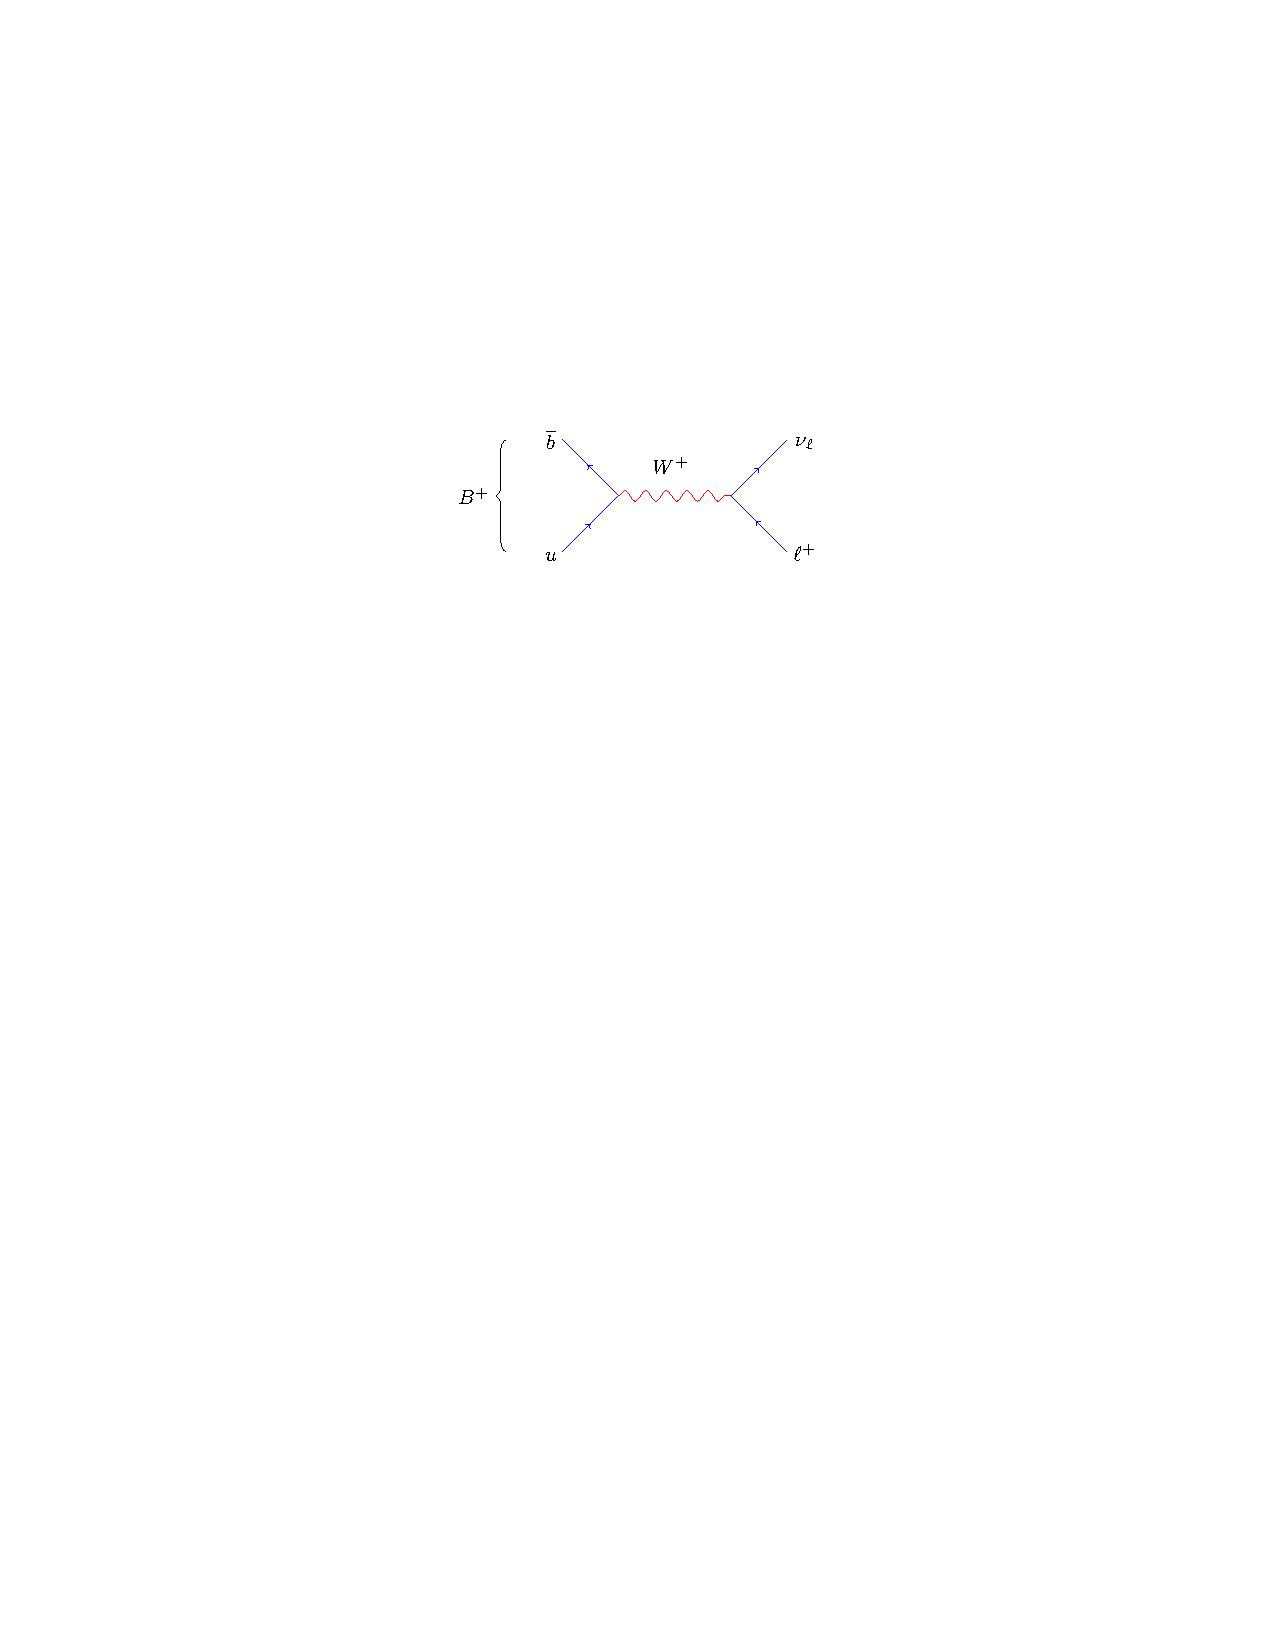
\includegraphics[width=0.5\textwidth]{figs/Theory/B2ellnu.pdf}
    \caption{Annihilation topology process for \decay{\Bp}{\ellp\neul} decays.}
    \label{fig:Theory_B2ellnu}   
\end{figure}
%%%%%%%%%%%%%%%%%%%%%%%%%%%%%%%%%%%%%%%%%%%%%%%%%%%%%%%%%%

\begin{table}[h]
   \begin{center}
      \begin{tabular}{lcc}
         \hline

         Decay Mode                 & SM prediction & Measurement \\
         \hline 
         \decay{\Bp}{\ep\neue}      & $(1.3\pm0.4)\times10^{-11}$           & $<9.8\times10^{-7}$\\
         \decay{\Bp}{\mup\neum}     & $(5.6\pm0.4)\times10^{-7}$            & $<1.0\times10^{-6}$\\
         \decay{\Bp}{\taup\neut}    & $(0.75^{+1.0}_{-0.05} )\times 10^{-4}$& $(1.09\pm0.24)\times 10^{-4}$ \\

         \hline
      \end{tabular}
   \end{center}
   \caption{Theoretical predictions and experimental measurements for \decay{\Bp}{\ellp\neul} processes, from Refs.~\cite{PhysRevD.92.051102,PhysRevD.79.091101,SATOYAMA200767}.}
   \label{tab:Theory_B2ellnu}
\end{table}
This purely leptonic \Bp meson decay can proceed to either of the three generations with the branching fractions detailed in Table~\ref{tab:Theory_B2ellnu}. The effect of helicity suppression in the final state is illustrated by the rapid decrease in predicted branching fraction as the mass charged lepton decreases. The neutrino in the final state makes this decay experimentally challenging to reconstruct at hadron colliders such as the \lhc. The measurement of \decay{\Bp}{\taup\neut} was performed at the \belle experiment, a \B-factory colliding \ep\en pairs at the $\PUpsilon(\text{4S})$ resonance. 
Hadronic annihilation decays are necessarily more complicated than these purely leptionic processes as the quark and antiquark must be further hadronised as they cannot remain bare.


{\color{Red}
\begin{itemize}
\item Talk about \D and other annihilation topologies 
\item Find origin of hadronic uncertainties 
\item \decay{\Bz}{\Kp\Km}? penguin annihilation
\end{itemize}}


\subsection{Pure annihilation topology decays}
Pure annihilation topology decays are an interesting subset of processes in which (at lowest order) only annihilation decay diagrams contribute. These are of particular interest because this allows the magnitudes of these processes to be isolated. Additionally, they provide a suitable forum in which to search for new physics; enhanced or decreased branching fractions and non-zero \CP violations are symptomatic of multiple competing processes interfering with one another.  

Typically, hadronic \emph{pure} annihilation processes are characterised by a mutually exclusive set of quarks in the initial and final state. This implies that the initial state must have completely annihilated into a mediator for this process to occur.   

{\color{Red}
\begin{itemize}
\item Pure annihilation - charmless Bc
\end{itemize}}

\subsection{Other annihilation decays}
Processes that don't uniquely proceed via annihilation decays are also of interest. 
{\color{Red}
\begin{itemize}
\item non pure - donals Bc 
\end{itemize}}

\section{Rescattering}

Rescattering allows \Bp mesons to decay to final states that are ideal pure annihilation topologies via an intermediate process of some other topology. This can potential limit the sensitivity the annihilation decay if these processes happen at a significant rate. Intermediate processes that could contribute to the \decay{\Bp}{\Dsp\phiz} decay are shown in Fig.~\ref{fig:Theory_rescattering}. These rather complicated processes both involve tree-level \decay{\bquarkbar}{\uquarkbar} transitions in which one of both of the products undergo a final state interactions.  

%%%%%%%%%%%%%%%%%%%%%%%%%%%%%%%%%%%%%%%%%%%%%%%%%%%%%%%%%%
\begin{figure}[!h]
    \centering
    \begin{subfigure}[m]{0.7\textwidth}
        \centering
        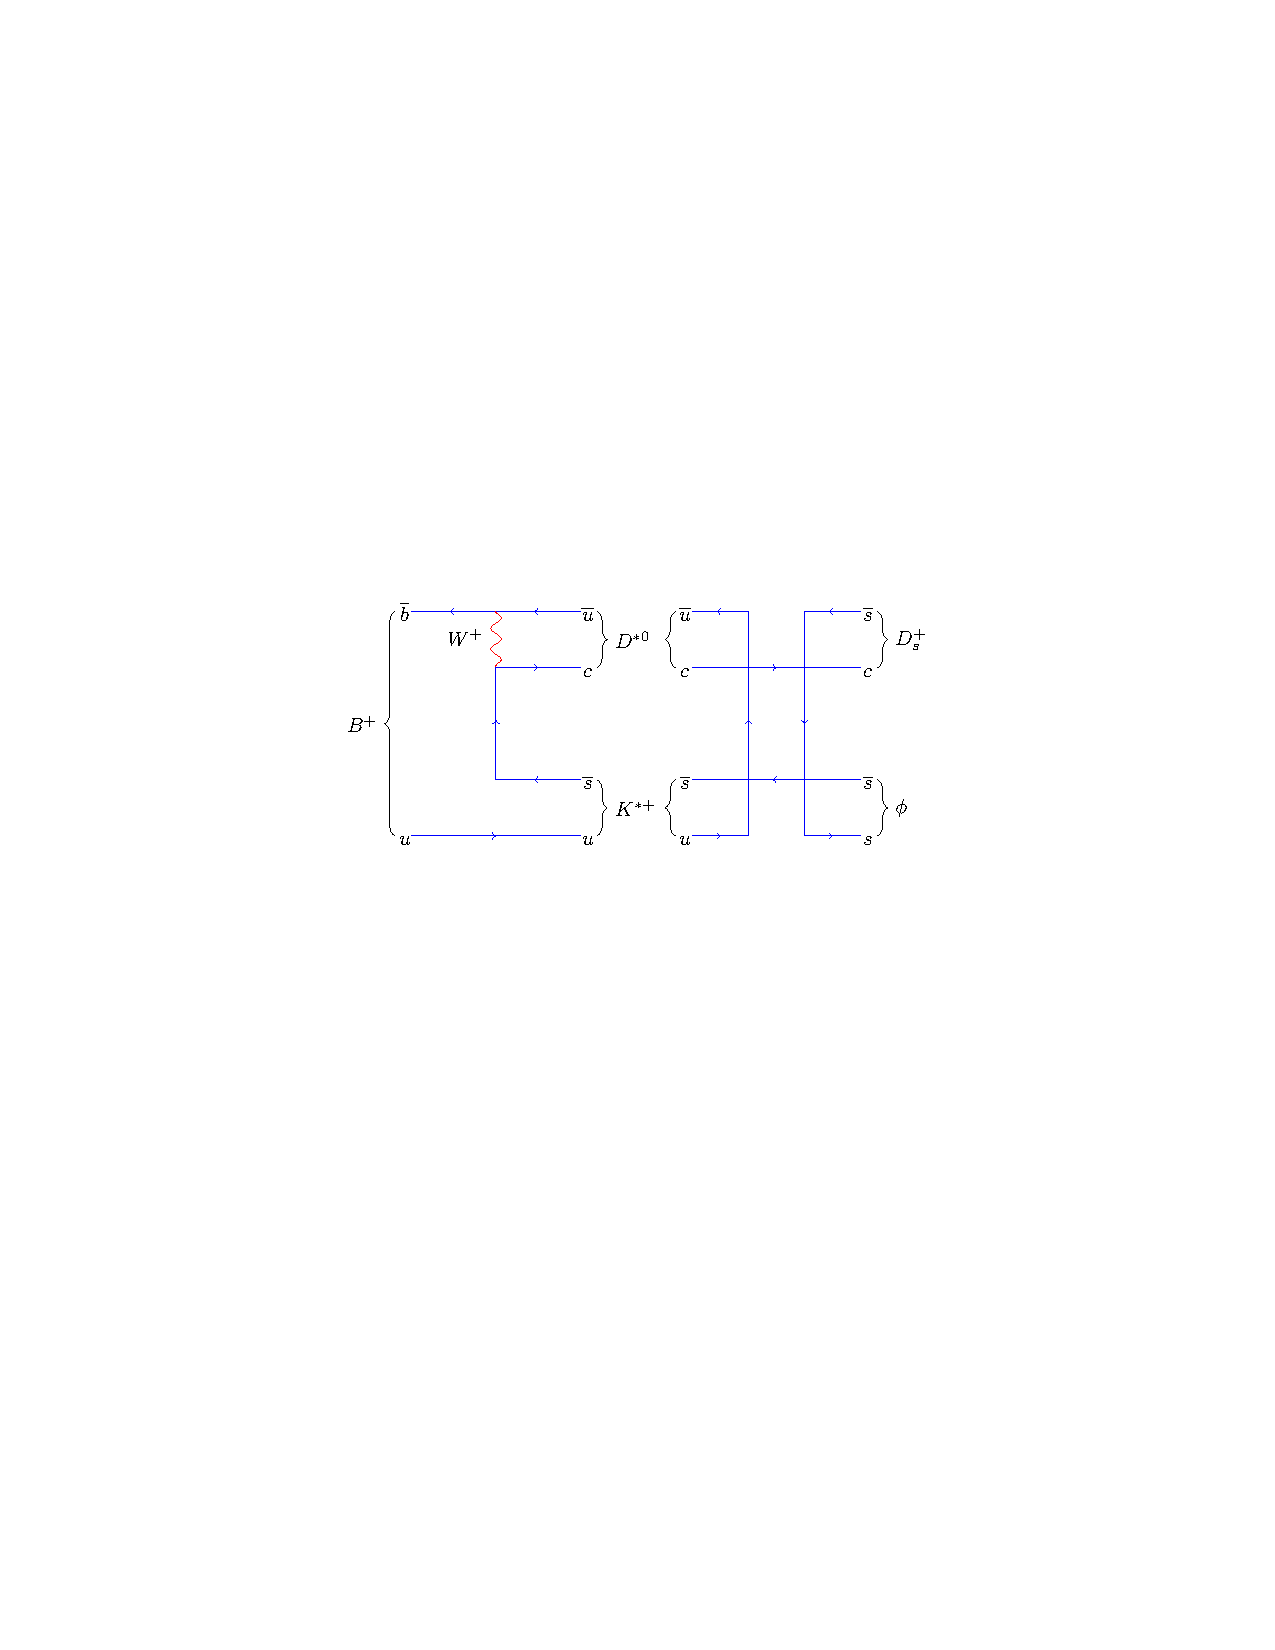
\includegraphics[width=1.0\textwidth]{figs/Theory/B2DsPhi_Rescattering_B2D0K.pdf}
        \caption{via \decay{\Bp}{\Dstarz\Kstarp}}
    \end{subfigure}
    \begin{subfigure}[m]{0.7\textwidth}
        \centering
        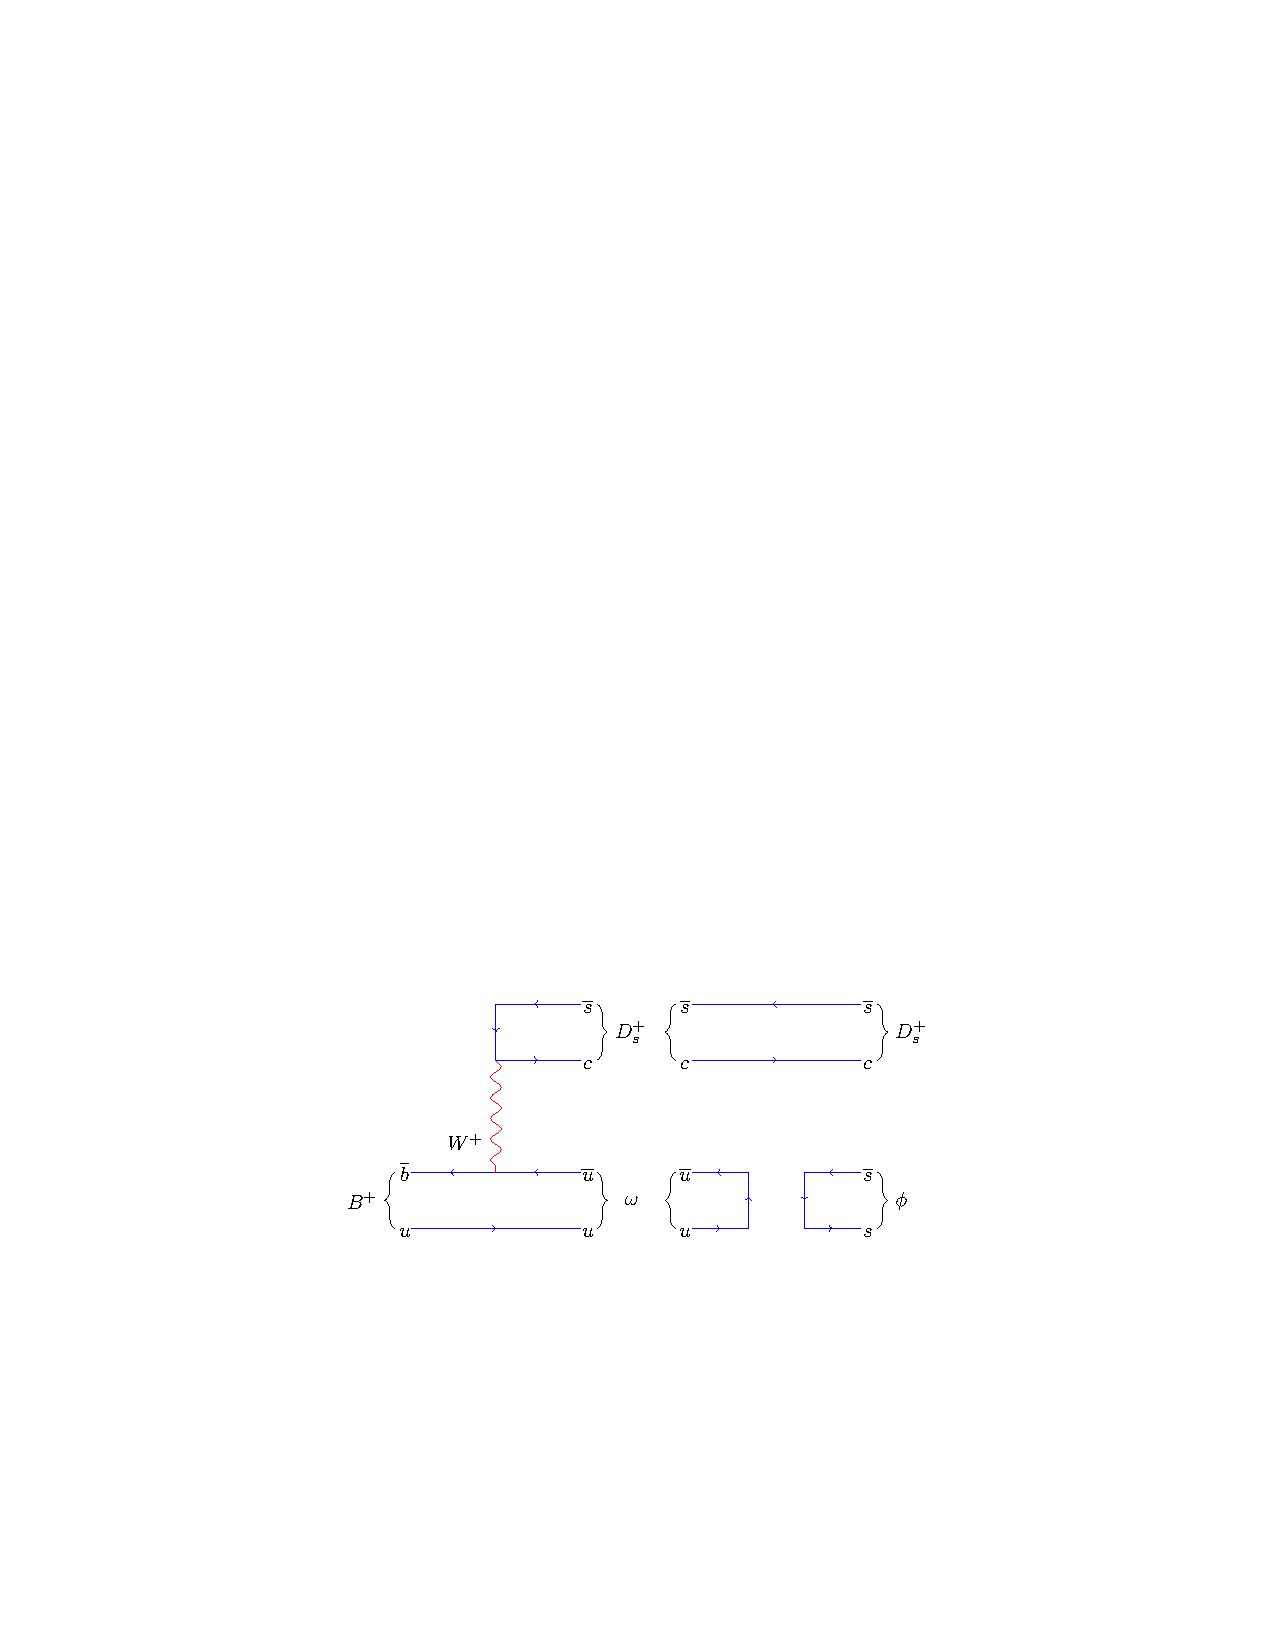
\includegraphics[width=1.0\textwidth]{figs/Theory/B2DsPhi_Rescattering_B2Dsomega.pdf}
        \caption{via $\decay{\Bp}{\Dsp\omega}$}
    \end{subfigure}
    \caption{Rescattering contributions to \decay{\Bp}{\Dsp\phiz} decays.}
    \label{fig:Theory_rescattering}   
\end{figure}
%%%%%%%%%%%%%%%%%%%%%%%%%%%%%%%%%%%%%%%%%%%%%%%%%%%%%%%%%%



{\color{Red}
\begin{itemize}
\item What is rescattering?
\item Examples of it?
\item Why it's expected to be small
\item $\decay{\Bu}{\Dsp\omega}$
\item $\omega\to\phi$ is OZI suppressed 
\item $\decay{\Bu}{\Dz\Kstarp}$
\item References: \Dp\Kstarz~\cite{Mehraban2016}.
\item $\omega - \phi$ mixing: ~\cite{OKUBO1963165,PhysRevD.79.074006}.

\end{itemize}}

\section{Theoretical predictions for the \decay{\Bp}{\Dsp\phiz} decay}

%%%%%%%%%%%%%%%%%%%%%%%%%%%%%%%%%%%%%%%%%%%%%%%%%%%%%%%%%%
\begin{figure}[!h]
    \centering
    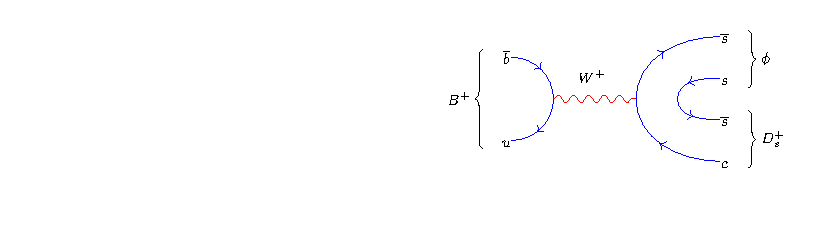
\includegraphics[width=0.6\textwidth]{figs/Theory/B2DsPhi.pdf}
    \caption{\decay{\Bp}{\Dsp\phiz} }
    \label{fig:Theory_DsPhiDiagram}   
\end{figure}
%%%%%%%%%%%%%%%%%%%%%%%%%%%%%%%%%%%%%%%%%%%%%%%%%%%%%%%%%%



{\color{Blue}
In the SM, the decay $\decay{\Bp}{\Dsp\phi}$ proceeds dominantly via the annihilation diagram shown in Fig.~\ref{fig:Theory_DsPhiDiagram}. 
This suppressed topology requires the wave functions of the incoming quarks to overlap sufficiently to annihilate into a virtual \Wp boson. 
The decay is further suppressed by the small magnitude of the CKM matrix element \Vub associated with the annihilation vertex. 


}

\subsection{Standard model predictions}
{\color{Blue}
Several SM predictions have been made for the branching fraction of the $\decay{\Bp}{\Dsp\phi}$ decay~\cite{Zou:2009zza, Mohanta:2002wf, Mohanta:2007uu, Lu:2001yz}, using input from lattice calculations~\cite{fB:2013HPQCD,fB:2016ETM, fB:2016Fermi}. These predictions are in the range $(1-7)\times10^{-7}$, where the limit on the precision is dominated by hadronic uncertainties. 

In addition, unlike many rare hadronic decays including $\decay{\Bp}{\Dsp\Kp\Km}$, possible contributions from rescattering effects are expected to be small, for example contributions from intermediate states such as $\decay{\Bp}{\Dsp\omega}$~\cite{Gronau:2012gs}.

}

{\color{Red}
\begin{itemize}
\item Find origin of hadronic uncertainties 
\end{itemize}}

\subsection{BSM models and predictions}
{\color{Blue}
However, additional diagrams contributing to this decay can arise in some extensions of the SM, such as supersymmetric models with R-parity 
violation. They could enhance the branching fraction and/or produce large \CP asymmetries~\cite{Mohanta:2002wf, Mohanta:2007uu}, which makes the $\decay{\Bp}{\Dsp\phi}$ decay a promising place to search for new physics beyond the SM.\footnote{Charge conjugation is implied throughout this paper. Furthermore, $\phi$ denotes the $\phi(1020)$ resonance.}
}

{\color{Red}
\begin{itemize}
\item Higgs doublet
\item SUSY 
\item include feynman diagrams
\item small intro into models
\end{itemize}}

\subsection{Previous measurements}

{\color{Blue}
The \lhcb experiment reported evidence for the decay $\decay{\Bp}{\Dsp\phi}$ using $pp$ collision data corresponding to an integrated luminosity of 1\invfb taken during 2011, at a centre-of-mass energy of 7\tev~\cite{Aaij:2012zh}. A total of $6.7^{+4.5}_{-2.6}$ candidates was observed. The branching fraction was determined to be 

\begin{equation}
\mathcal{B}(\decay{\Bp}{\Dsp\phi}) = (1.87^{+1.25}_{-0.73} \pm 0.19 \pm 0.32) \times 10^{-6},
\end{equation}
where the first uncertainty is statistical, the second is systematic and the third is due to the uncertainty on the branching fraction of the decay $\decay{\Bp}{\Dsp\Dzb}$, which was used as normalisation. 
Given the large uncertainties on both the theoretical and experimental values, the previously measured value is consistent with the range of SM values given above.
}

{\color{Red}
\begin{itemize}
\item Include plot and measurement
\item say something about similarites 
\end{itemize}}


\section{Theoretical predictions for the \decay{\Bp}{\Dsp\Kp\Km} decay}


%%%%%%%%%%%%%%%%%%%%%%%%%%%%%%%%%%%%%%%%%%%%%%%%%%%%%%%%%%
\begin{figure}[!h]
    \centering
    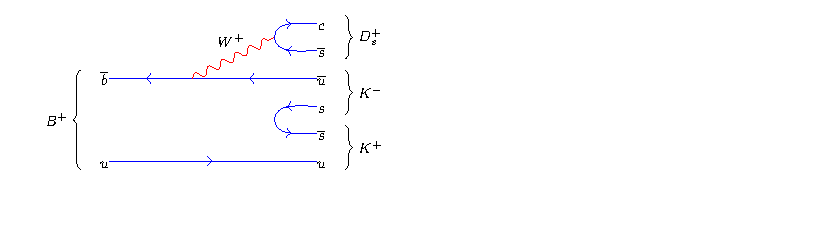
\includegraphics[width=0.6\textwidth]{figs/Theory/B2DsKK.pdf}
    \caption{\decay{\Bp}{\Dsp\Kp\Km} }
    \label{fig:Theory_DsKKDiagram}   
\end{figure}
%%%%%%%%%%%%%%%%%%%%%%%%%%%%%%%%%%%%%%%%%%%%%%%%%%%%%%%%%%



{\color{Blue}
The decay $\decay{\Bp}{\Dsp\Kp\Km}$ is mediated by a $\decay{\bquarkbar}{\uquarkbar}$ transition shown in Fig.~\ref{fig:Theory_DsKKDiagram} and is therefore suppressed in the Standard Model (SM) due to the small size of the Cabibbo-Kobayashi-Maskawa (CKM) matrix element \Vub. 
}


{\color{Red}
\begin{itemize}
\item explain what a dalitz plot is
\end{itemize}
}

\subsection{Standard model predictions}
{\color{Blue}
The branching fraction for this decay is currently not measured, however a similar decay, \decay{\Bp}{\Dsp \piz}, has been observed with a branching fraction of $\mathcal{B}(\decay{\Bp}{\Dsp \piz}) = (1.5 \pm 0.5) \times 10^{-5}$~\cite{Aubert:2006xy}.
}


{\color{Red}
\begin{itemize}
\item talk about \decay{\Bp}{\Dsp\piz}
\item Could talk about \decay{\Bp}{\Dp\Kp\pim} and estimate   
\end{itemize}}

\subsection{Previous measurements}




\chapter{The \lhcb experiment} 
\label{ch:detector}
\minitoc
 


\section{\cern and the \lhc}


In the aftermath of the Second World War a number of eminent scientists proposed the creation of a collaborative European laboratory dedicated to the study of atomic physics. With this the `Conseil Europ\'een pour la Recherche Nucl\'eaire' was born; a provisional council set up in 1952 to oversee the laboratory's creation.  In 1954 the organisation as it is today was established, named the `Organisation Europ\'eenne pour la Recherche Nucl\'eaire', although the acronym \cern remained. 
The purpose of \cern was clear; the convention dictates that the organisation \emph{`shall provide for collaboration among European States in nuclear research of a pure scientific and fundamental character'}.
As such 

Furthermore, the convention stipulates that the organisation \emph{`shall have no concern with work for military requirements'} and  
requires \emph{`the results of its experimental and theoretical work shall be published or otherwise made generally available'}. 
The choice of the laboratories location followed a similar set of values, picking Geneva in Switzerland owing both to the central European location and neutrality of the host state. 


Perhaps the most well known accelerator in the complex [cite something], \cern is home to the Large Hadron Collider (\lhc). Two beams of hadrons circulate in opposite directions around 27\km rings, colliding at four interaction points. The beam pipes and experimental halls are buried deep underground, providing shielding from radiation and reducing the cost of acquiring large areas of land. The tunnels traverse the Franco-Swiss border at a depth that varies between 50--175\m at the lowest and highest points respectively.      


{\color{Red}
\begin{itemize}
\item Founding of \cern and a little history 
\item LEP was in tunnel before
\item Mission statement
\item Notable results and and contributions to society
\item Mention experiments other than those attached to accelerator complex
\item Time line
\item running periods? and future plans...
\end{itemize}
}

\subsection{The accelerator complex}

The \lhc is only one of a vast collection of accelerators at \cern, albeit the largest. The hadrons collided in the \lhc travel sequentially through a number of different machines, boosting their momentum in each. The full complex is shown in Fig.~\ref{fig:Dec_lhcb_Schematic} along with a legend detailing the types of particles considered. The protons begin life in a hydrogen gas canister. The gas is ionised and accelerated in  a linear accelerator, LINAC2, to an energy of 50\mev. These then pass into the Proton Synchrotron Booster, raising the energy further from 50\mev to 1.4\gev. 

In addition to protons, the complex can accelerate other ions including lead, and more recently, argon and xenon {\color{Red}cite}. These start in a dedicated linear accelerator, LINAC3, where the ions are stripped to bare nuclei before being injected into the Low Energy Ion Ring (LEIR). This ring raises the ion's energy from 4.2\mev to 72\mev. 

Either protons or ions can then be injected in the Proton Synchrotron (PS), \cern's first synchrotron. Once the world's highest energy particle accelerator, this now accelerates the particles up to 25\gev ready to be injected into the Super Proton Synchrotron (SPS).
The SPS is the second largest accelerator at \cern, with a circumference of 7\km. It was switched on in 1976 and resulted in the notable discoveries of the \W and \Z bosons. Here, the particles are accelerated up to an energy of 450\gev. 

%%%%%%%%%%%%%%%%%%%%%%%%%%%%%%%%%%%%%%%%%%%%%%%%%%%%%%%%%%
\begin{figure}[!h]
    \centering
    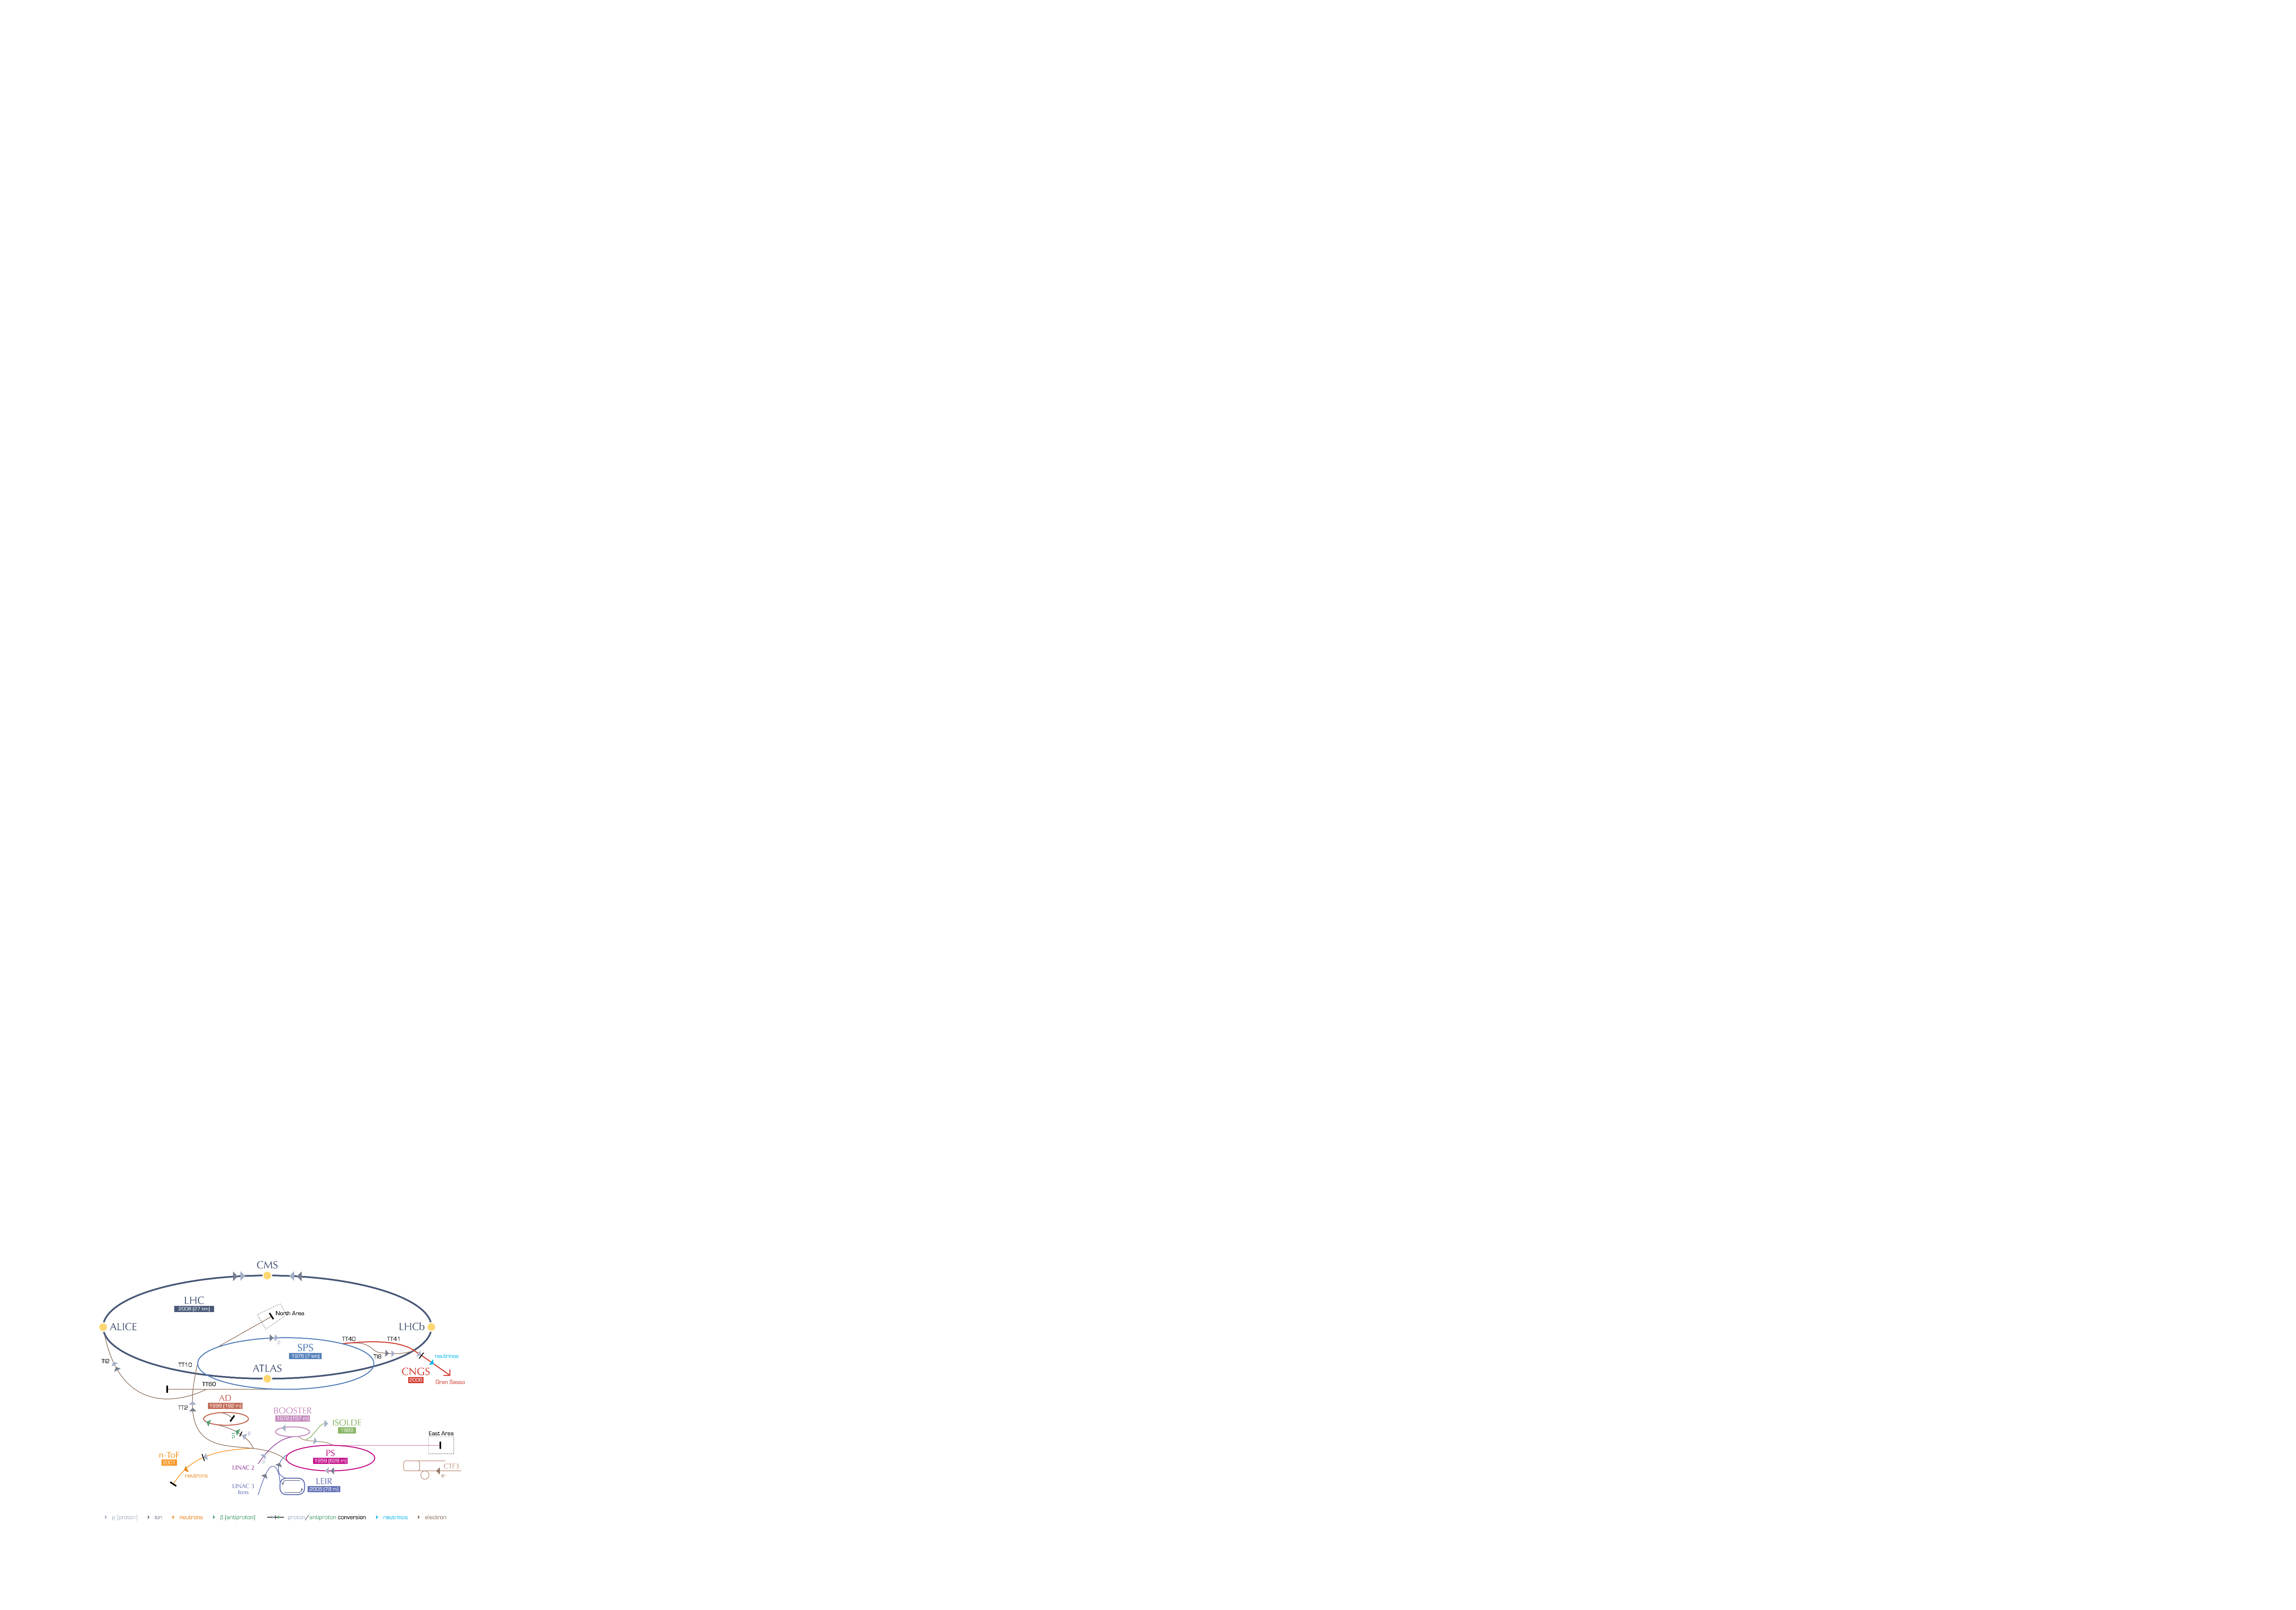
\includegraphics[width=1.0\textwidth]{figs/Detector/Acc_complex.pdf}
    \caption{The accelerator complex at \cern taken from Ref...}
    \label{fig:Dec_Acc_Complex}   
\end{figure}
%%%%%%%%%%%%%%%%%%%%%%%%%%%%%%%%%%%%%%%%%%%%%%%%%%%%%%%%%%



{\color{Red}
\begin{itemize}
\item Brief overview of the life of a proton from source to \lhc
\item injected into two beams
\item injection points
\item Phases of \lhc?
\end{itemize}
}

\subsection{The \lhcb collaboration} 
A total of seven experiments are located at the \lhc, situated in four caverns. The four largest are \atlas, \cms, \lhcb and \alice. The TOTEM, LHCf and MoDEL experiments are located in the same caverns as \cms, \atlas and \lhcb respectively. 

The \lhcb collaboration is made up of around 800 scientists 


{\color{Red}
\begin{itemize}
\item People and counties 
\item physics aims?
\end{itemize}
}
\subsection{Beam conditions at \lhcb}
{\color{Red}
\begin{itemize}
\item \lhc optics
\item crossing angle
\item Luminosity levelling
\end{itemize}
}


\section{The \lhcb detector}

This section provides an overview of the experimental apparatus used to obtain the data analysed in this thesis.
The \lhcb detector is comprised of distinct sub-detectors, each with a dedicated purpose. These help to characterise the sub-atomic particles created in the proton-proton collisions, and enable measurements of their kinematics, trajectories and species.
This overview includes a description of the sub-detector's construction, components and performance. 

The \lhcb detector is found at Point 8 of the \lhc ring, a cavern originally built for the {\color{Red}\delphi} detector during the \lep era. A schematic representing the key components of the \lhcb detector is shown in Fig.~\ref{fig:Dec_lhcb_Schematic}. This figure displays the axes convention adopted by \lhcb, and used henceforth. The horizontal axis is labelled the $z$-axis and is parallel to the direction of the beams. The figure's vertical axis is the $y$-axis, increasing as one moves from the cavern up to ground level. The $x$-axis is in the dimension perpendicular to the plane of the figure. The $x$-axis increases as one moves towards the centre of the \lhc ring. The counter-rotating beams of protons are collided at the far left of this figure, at the origins of the $y$- and $z$-axes.   

%%%%%%%%%%%%%%%%%%%%%%%%%%%%%%%%%%%%%%%%%%%%%%%%%%%%%%%%%%
\begin{figure}[!h]
    \centering
    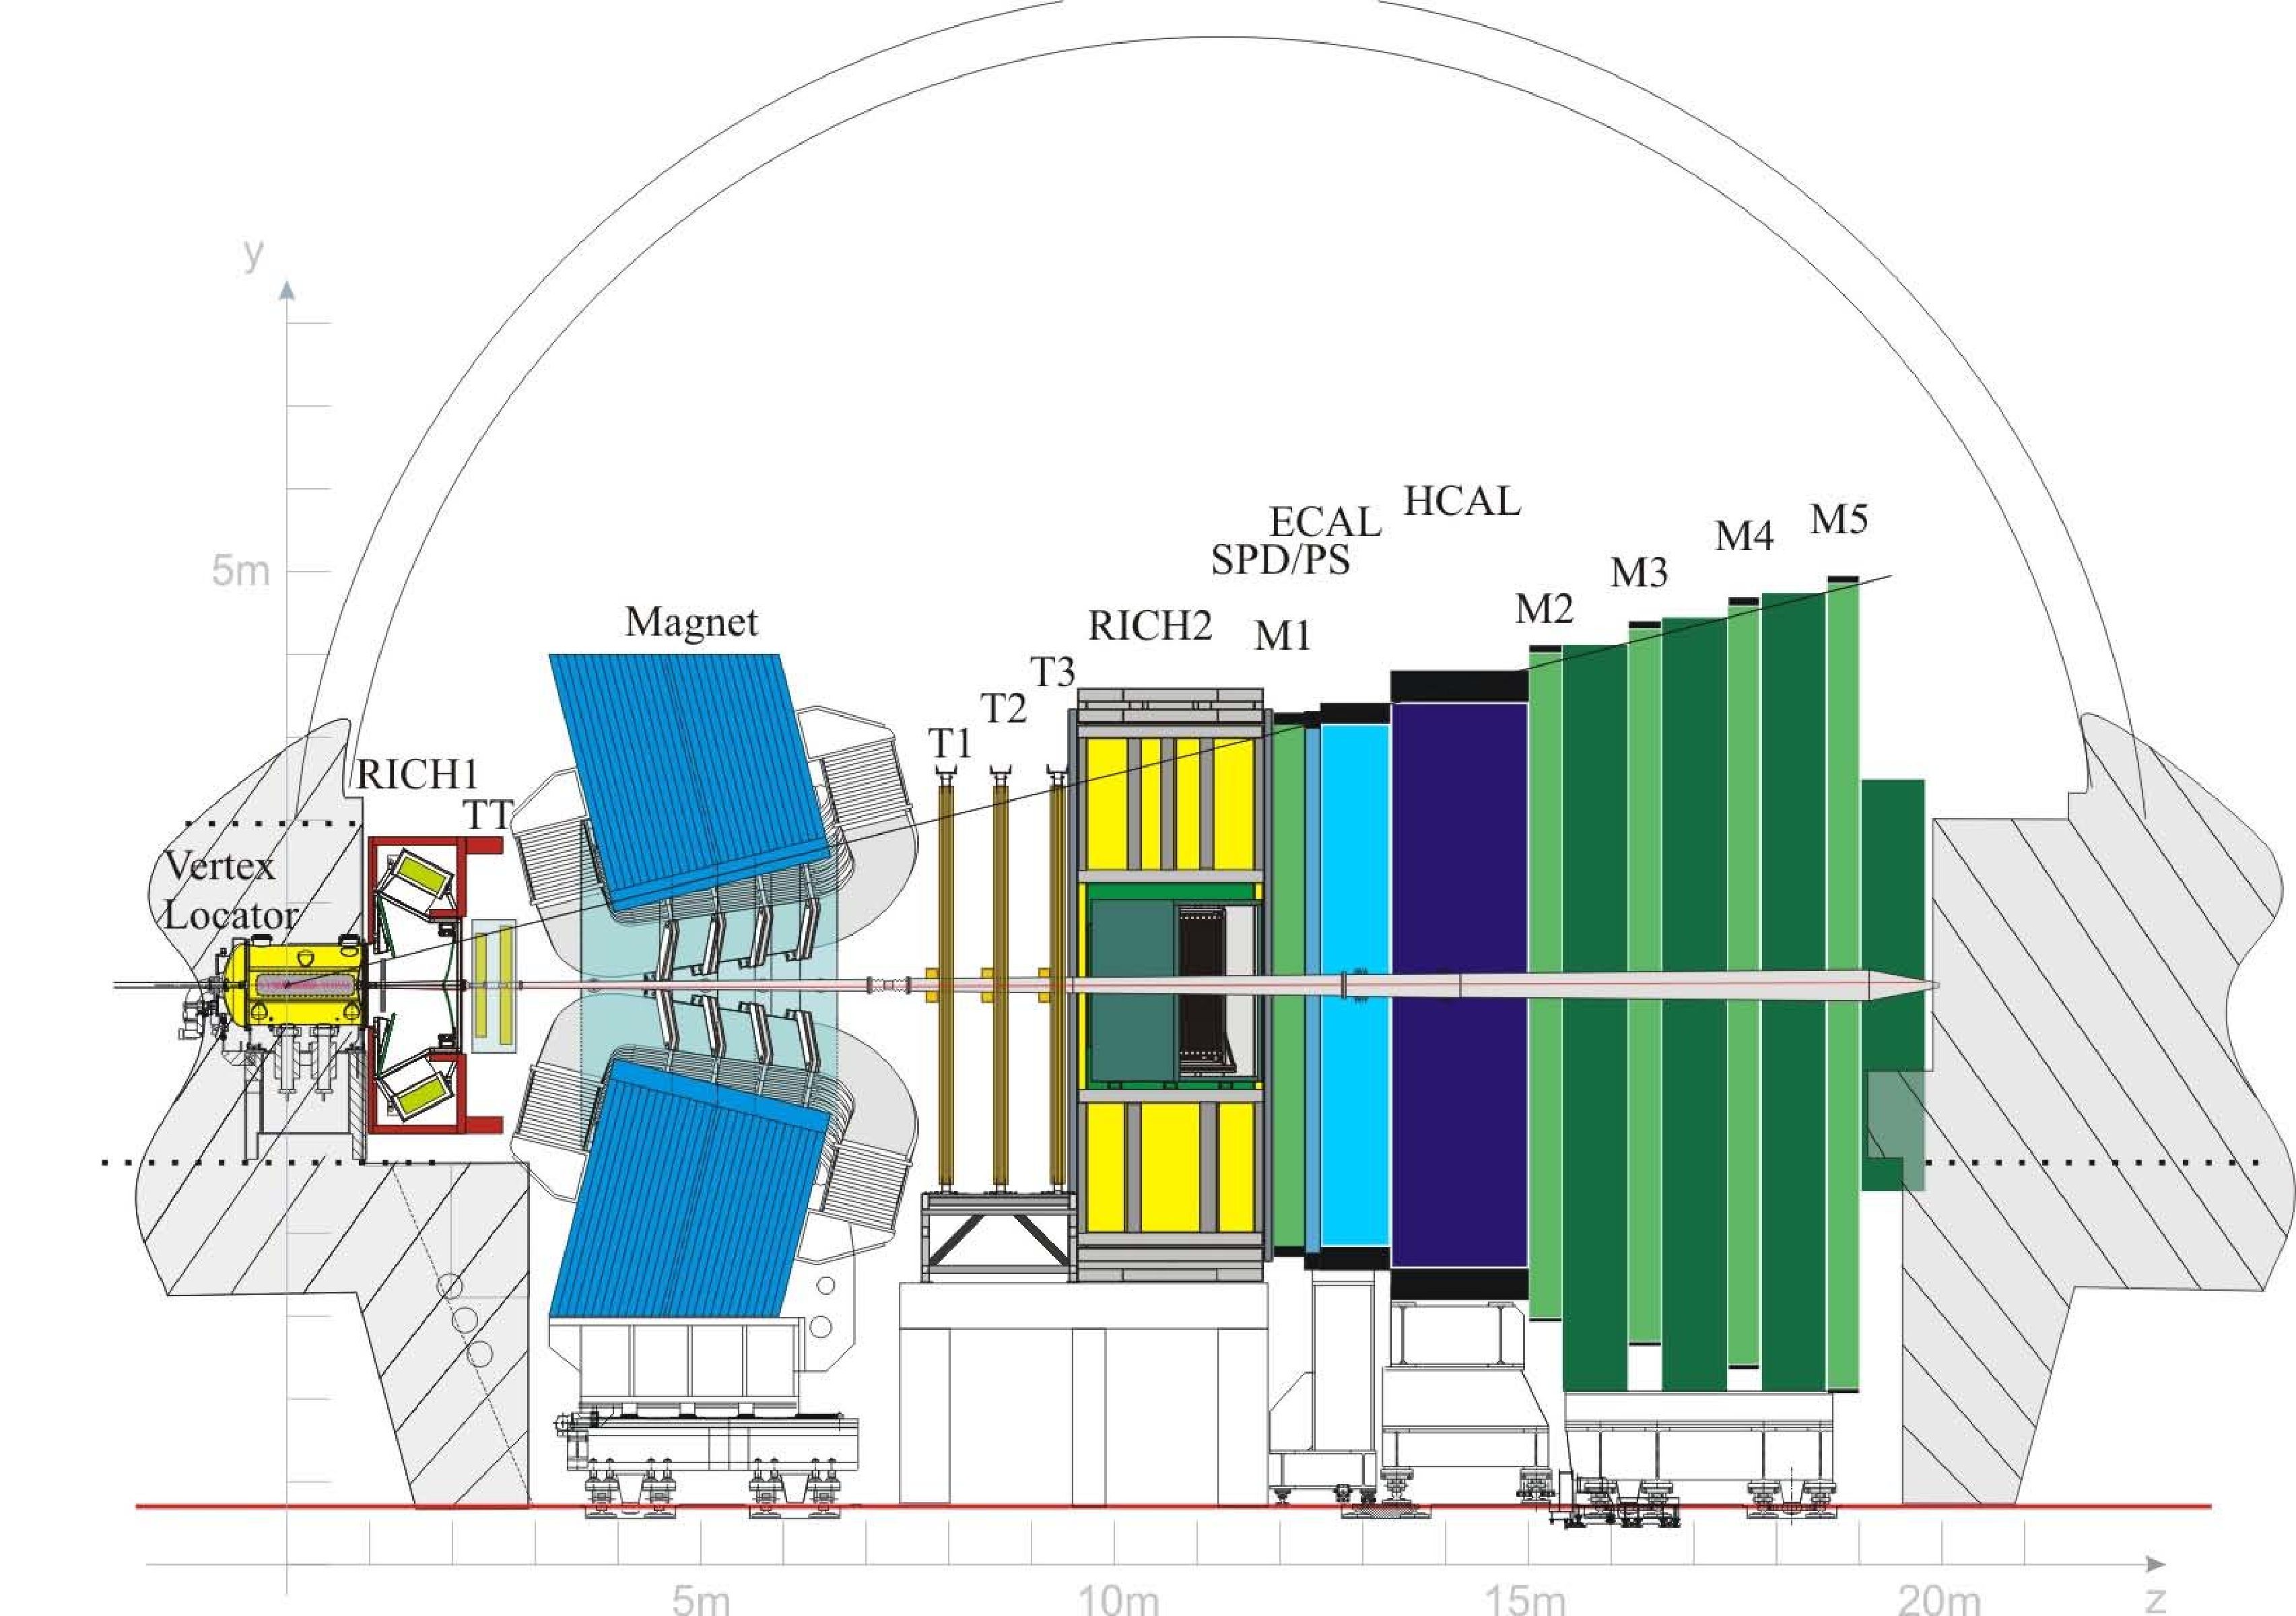
\includegraphics[width=0.8\textwidth]{figs/Detector/LHCb_Detector_Schematic.pdf}
    \caption{Schematic of the \lhcb detector, from Ref.~\cite{Alves:2008zz}.}
    \label{fig:Dec_lhcb_Schematic}   
\end{figure}
%%%%%%%%%%%%%%%%%%%%%%%%%%%%%%%%%%%%%%%%%%%%%%%%%%%%%%%%%%



Running along the centre of the detector is the \lhcb beampipe. The primary role is to separate the inner vacuum chamber from the rest of the cavern, allowing the beams to proceed unimpeded by the air. The majority of the beampipe is made of beryllium, with smaller sections made out of aluminium alloys or stainless steel. Although beryllium is a highly toxic and fragile material it has a long radiation length, allowing the incident particles to traverse the pipe walls with minimal interactions.  


{\color{Green}
\begin{itemize}
\item Distribution of bb pairs
\end{itemize}
}

\subsection{Magnet}

The \lhcb detector contains a warm dipole magnet that bends the trajectories of charges particles, allowing measurements of the particles' momentum. The magnet has two saddle-shaped coils inside a square yoke that generate an integrated magnetic field of 4 Tm.  
The magnetic field is aligned along the $y$-axis, bending the charged particles in the horizontal plane. The polarity of the magnetic is routinely switched during data taking. This helps to understand and cancel systematic effects that may affect measurements of \CP asymmetries. The two magnet polarities are referred to \emph{MagDown} and \emph{MagUp}, corresponding to a field in the negative and positive $y$-axis direction respectively.   

A schematic of the magnet is shown in Fig.~\ref{fig:Dec_magnet}, along with the strength of the magnetic field as a function of the $z$-axis position. Both magnet polarities are represented in this figure. 

{\color{Red}
\begin{itemize}
\item Magnet: purpose and design 
\end{itemize}
}


%%%%%%%%%%%%%%%%%%%%%%%%%%%%%%%%%%%%%%%%%%%%%%%%%%%%%%%%%%
\begin{figure}[!h]
    \centering
    \begin{subfigure}[t]{0.4\textwidth}
        \centering
        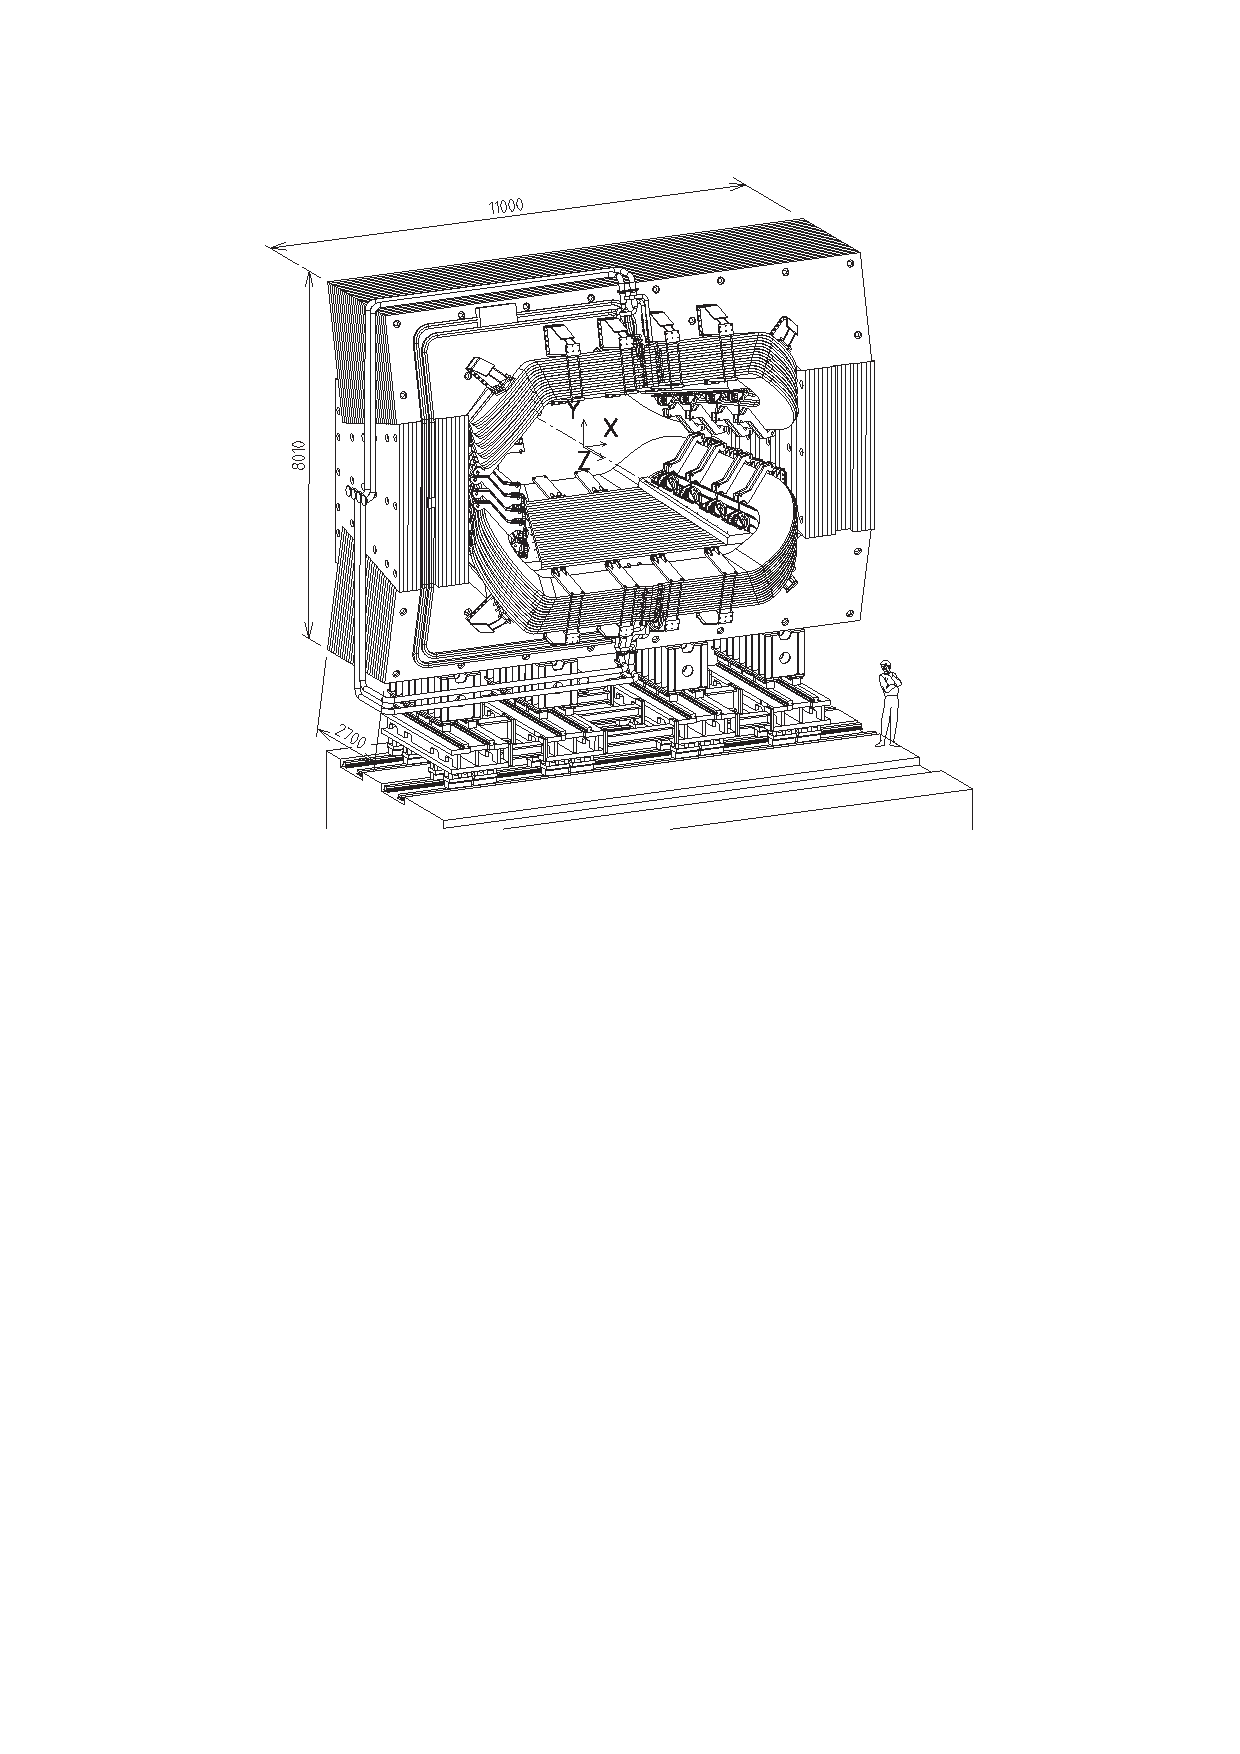
\includegraphics[width=1.0\textwidth]{figs/Detector/magnet_schematic.pdf}
    \end{subfigure}
    \begin{subfigure}[t]{0.4\textwidth}
        \centering
        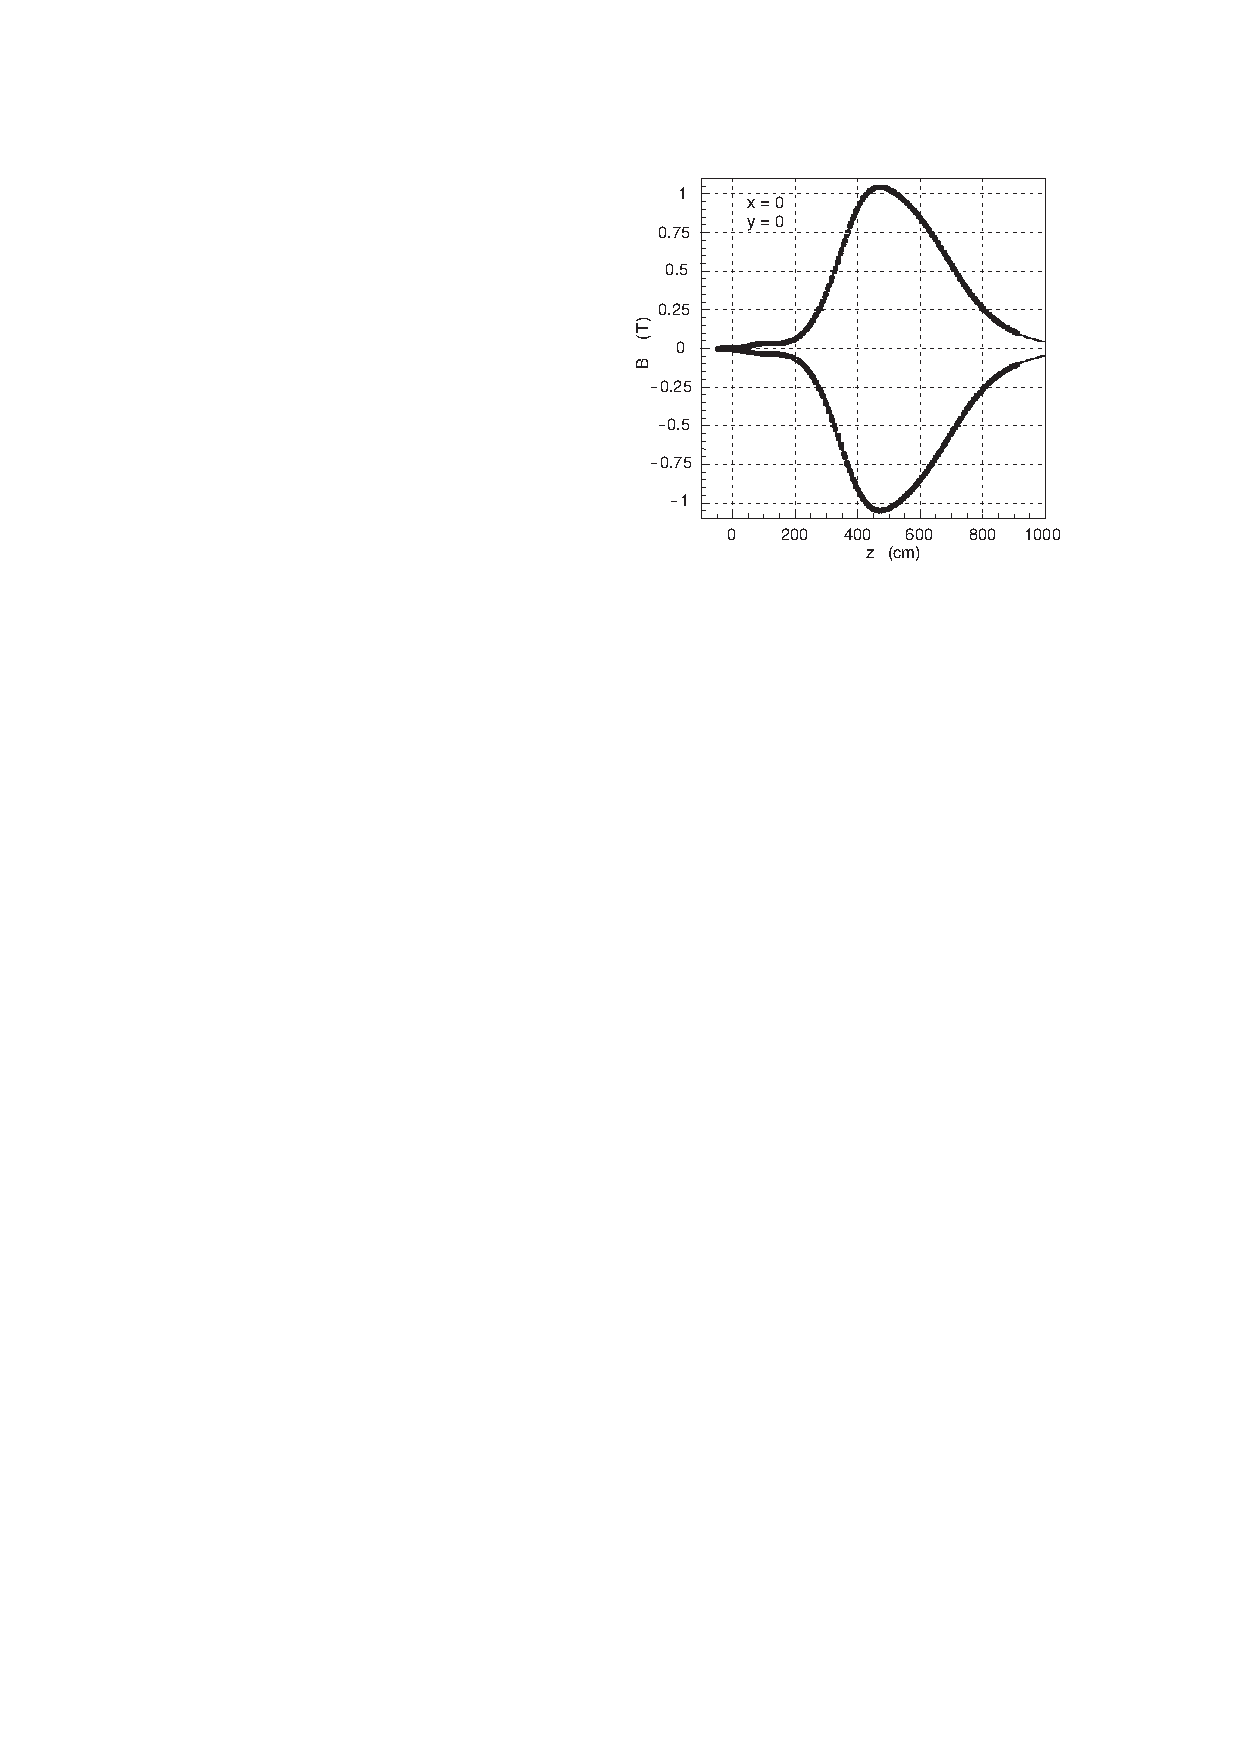
\includegraphics[width=1.0\textwidth]{figs/Detector/magnet_B_field.pdf}
    \end{subfigure}
    \caption{Schematic of the \lhcb warm dipole magnet (left) and the magnetic field strength along the $z$-axis (right) from Ref.~\cite{Alves:2008zz}.}
    \label{fig:Dec_magnet}   
\end{figure}
%%%%%%%%%%%%%%%%%%%%%%%%%%%%%%%%%%%%%%%%%%%%%%%%%%%%%%%%%%


\subsection{Vertex Locator}

The first sub-detector to make measurements of the particles produced in proton-proton collisions is the Vertex Locator (\velo) encompassing the collision region. This sub-detector make precise measurements of the track positions of charged particles as they emanate out of the collisions. A high level of precision is required to identify the secondary vertices characteristic of \bquark- and \cquark-hadron decays. These secondary vertices are typically displaced from the interaction position as a result of the long lifetimes associated to these heavy-flavour hadrons. This is achieved by measuring the track coordinates using silicon sensors placed a close to the \lhc beam as safety allows. The \velo sensors are semicircular devices placed on either side of the beam. To allow the sensors to instrument the innermost region around the interaction point the two halves of the \velo can move horizontally in and out. During normal data taking this allows the sensors to be 7\mm away from the interaction point yet still be a safe distance away from the beams at injection. 

%%%%%%%%%%%%%%%%%%%%%%%%%%%%%%%%%%%%%%%%%%%%%%%%%%%%%%%%%%
\begin{figure}[!h]
    \centering   
    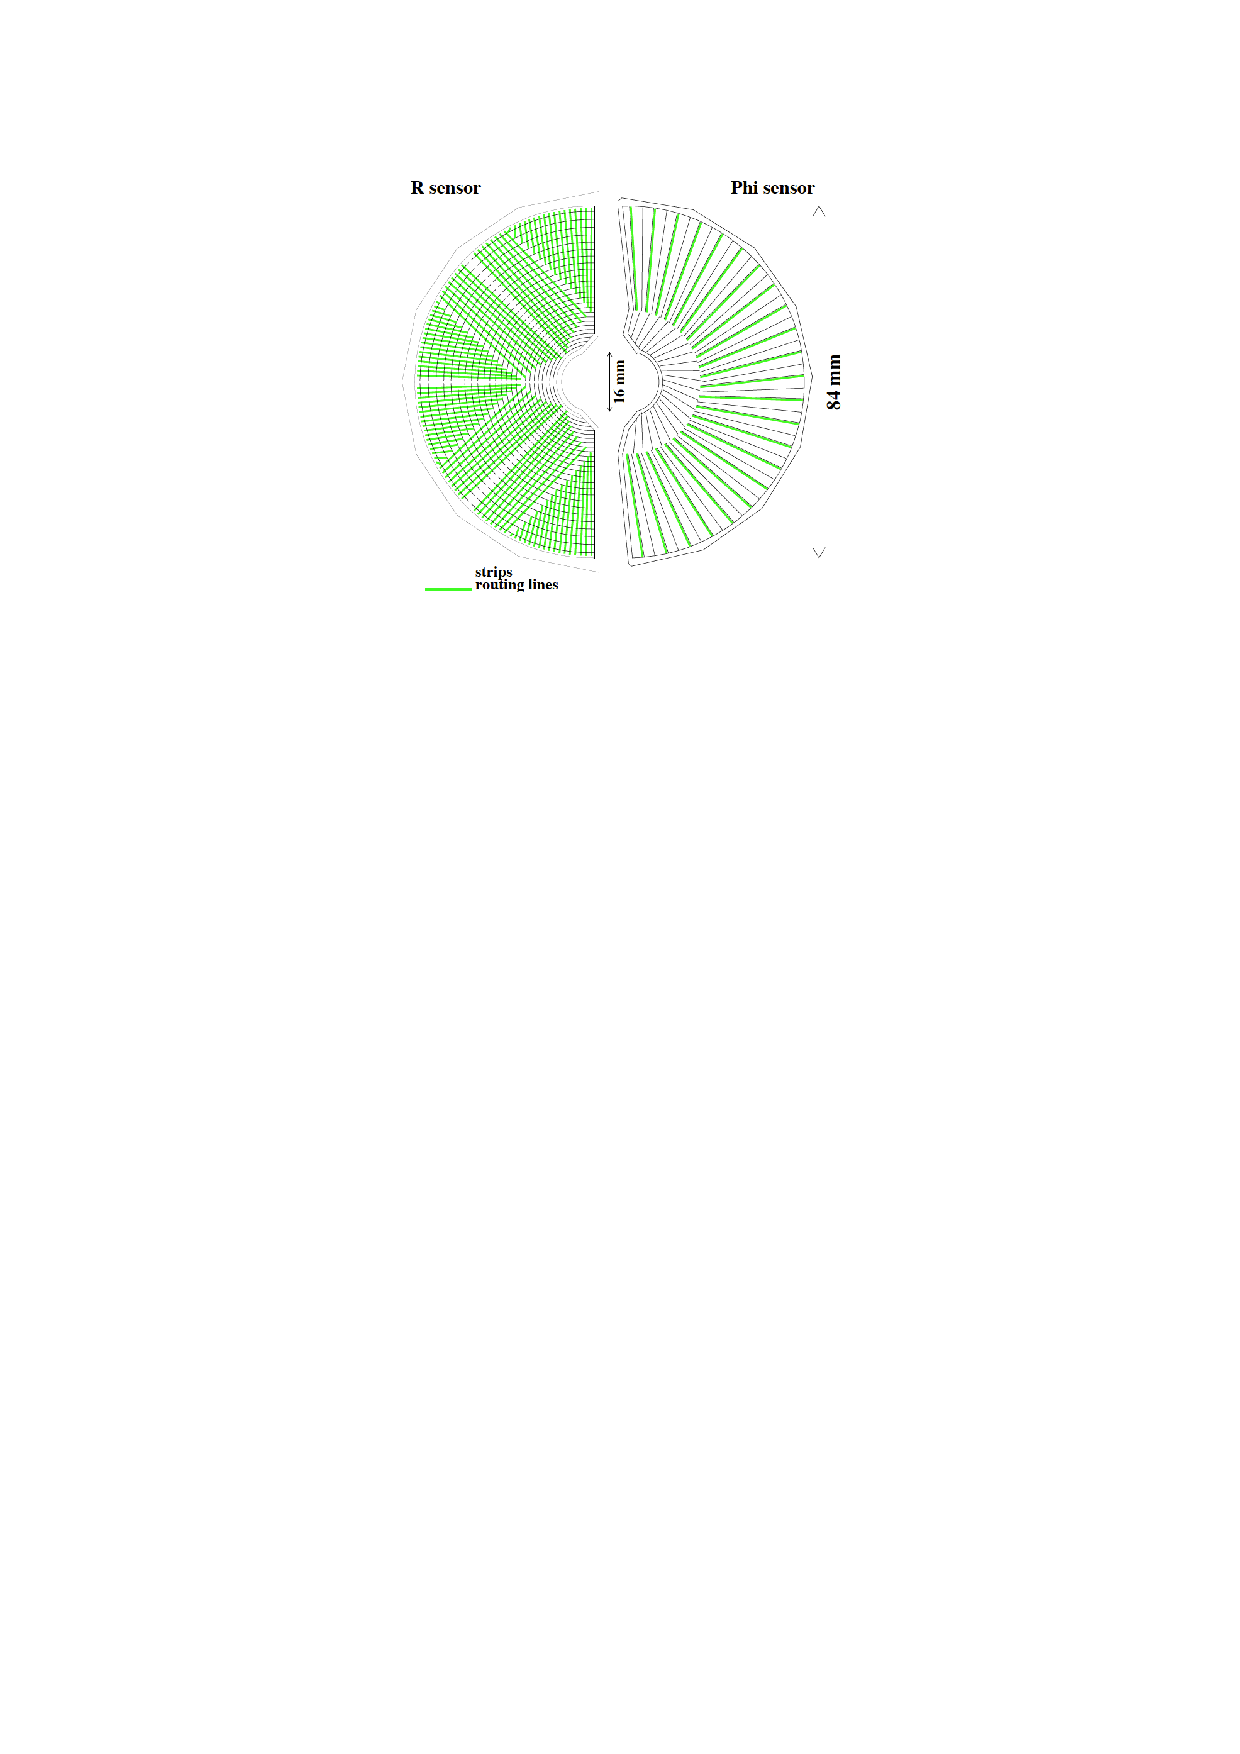
\includegraphics[width=0.4\textwidth]{figs/Detector/velo_r_phi_sensor.pdf}
    \caption{Schematic of an $r$- and $\phi$-sensor in the \velo sub-detector, from Ref.~\cite{LHCb-DP-2014-001}.}
    \label{fig:Dec_r_phi_sensor}   
\end{figure}
%%%%%%%%%%%%%%%%%%%%%%%%%%%%%%%%%%%%%%%%%%%%%%%%%%%%%%%%%%

The sensors are grouped into pairs, called modules. Each of the 21 modules on each side contains sensors for measuring the radial and azimuthal coordinates of the tracks, referred to as $r$- and $\phi$-sensors respectively. A schematic of the two sensor types is shown in Fig.~\ref{fig:Dec_r_phi_sensor}, illustrating the silicon strips and readout channels. 


The \velo modules are arranged to ensure coverage of particles emerging in forward region at angles of 15--300\mrad. The arrangement allows tracks within this acceptance to interact in at least three sensors as shown in Fig.~\ref{fig:Dec_velo_sensor_layout}.   
The modules extend both forward and backwards of the interaction region. Although momentum measurements are not possible for backward tracks, the vertexing of the primary interaction can benefit from this extra information. In the far backward region there are two additional modules, measuring only the radial coordinate. These help to identify pile-up events in which there is more than one primary vertex. 

%%%%%%%%%%%%%%%%%%%%%%%%%%%%%%%%%%%%%%%%%%%%%%%%%%%%%%%%%%
\begin{figure}[!h]
    \centering
    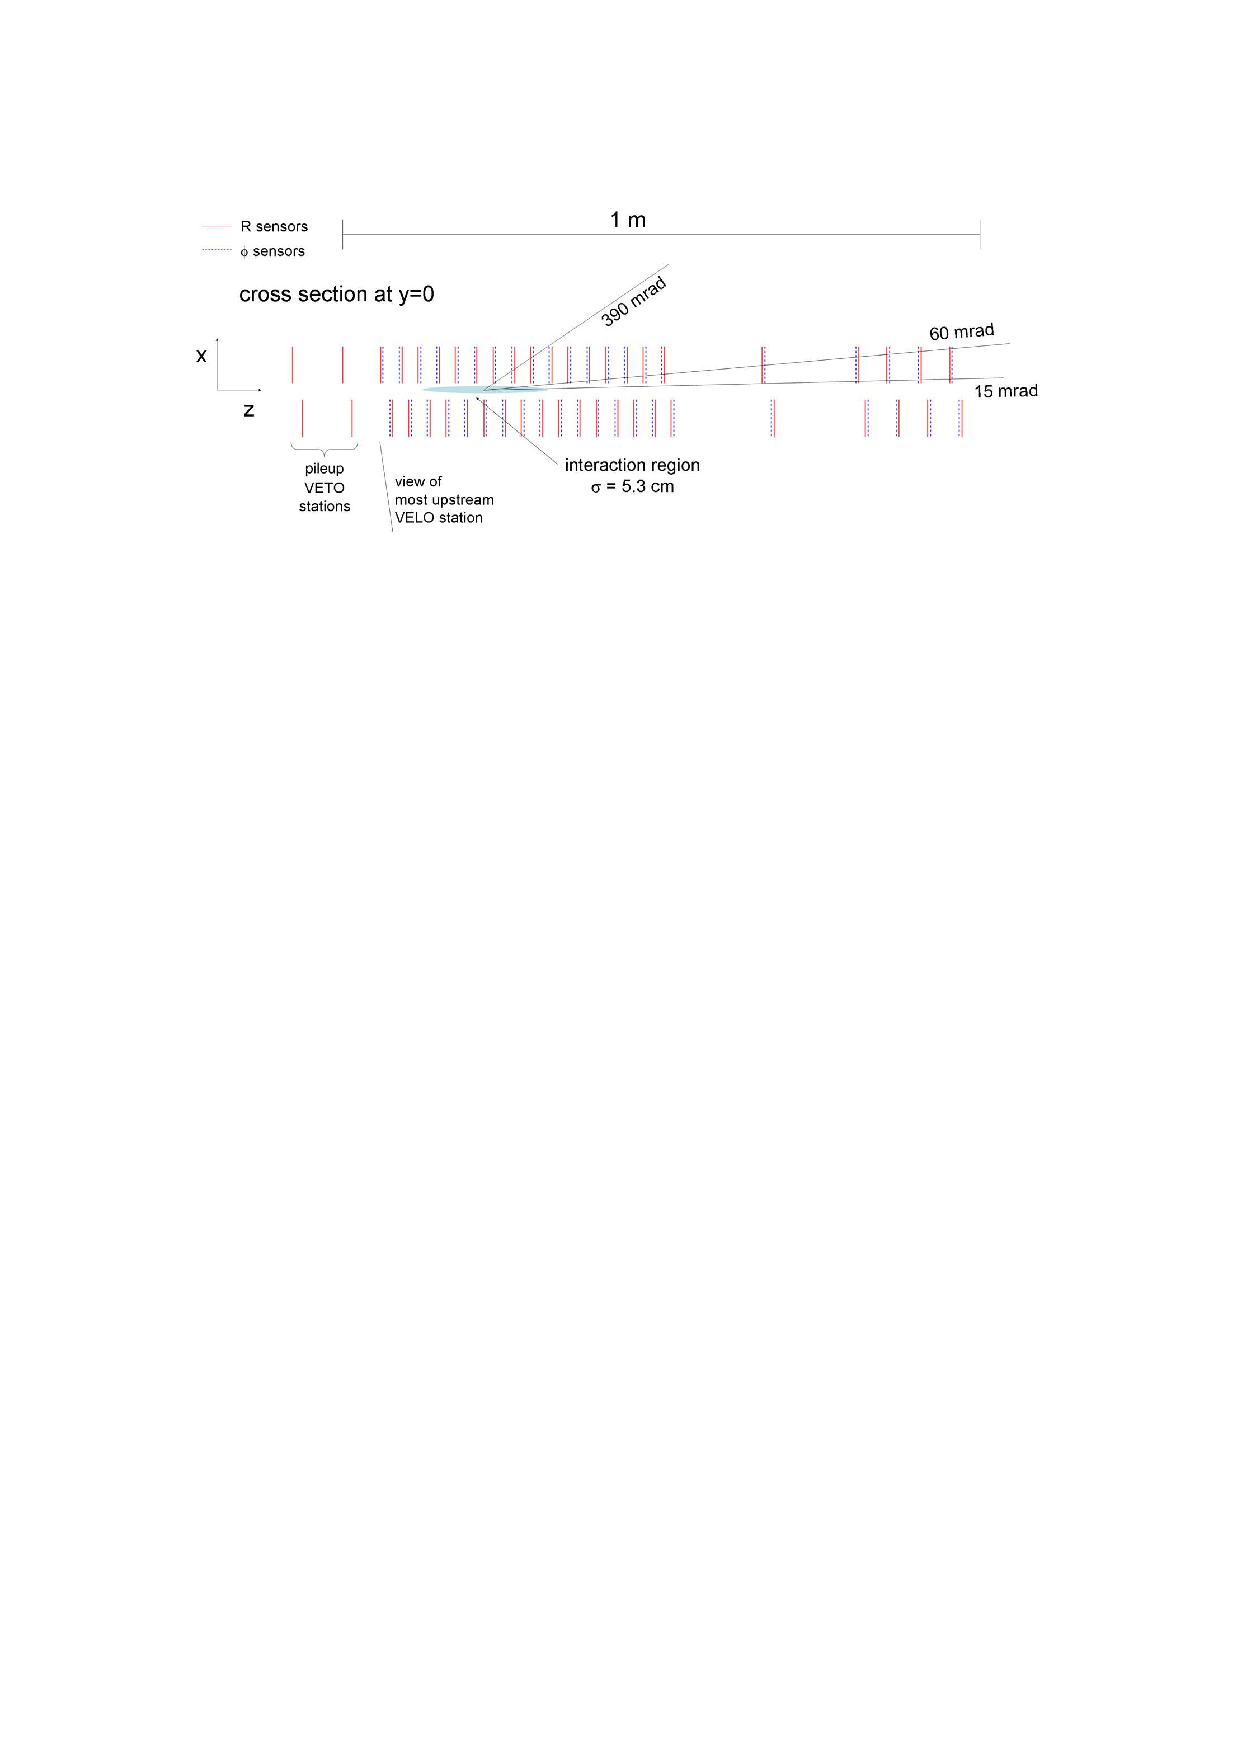
\includegraphics[width=0.8\textwidth]{figs/Detector/velo_sensor_layout.pdf}
    \caption{Schematic of the sensor layout in the \velo sub-detector, from Ref.~\cite{LHCb-DP-2014-001}.}
    \label{fig:Dec_velo_sensor_layout}   
\end{figure}
%%%%%%%%%%%%%%%%%%%%%%%%%%%%%%%%%%%%%%%%%%%%%%%%%%%%%%%%%%

The \velo sub-detector is constructed to operate in the unique environment close to the \lhc beams.

\begin{description}   
\item \textbf{Radiation resistance:} the \velo modules are subjected to extreme and varying amounts of radiation. The detector is designed to with stand three years of nominal \lhc running, using a radiation tolerant semiconductor construction. Additionally, the \velo modules are cooled to remove the heat created from the interactions. The sensors are maintained at a temperature between -10 and 0\degrees\,C with 24\,W of heat removed from each sensor.  
\item \textbf{Radio-frequency (RF) pick-up protection:} the electromagnetic fields generated by the \lhc beams could cause interference in the \velo detectors electronics. Therefore, a shield is used between the modules and the beam-pipe referred to as the RF-foil. This 0.3\mm thick foil separates the \velo and beam-pipe vacuums, providing additional protection to the conditions of the beams from the detector.
\end{description}   

The hits arising from particle interactions in the \velo sensors are extracted from the readout channels using custom analogue \beetle chips. The signals are digitised and combined into clusters in \tell1 readout boards~\cite{HAEFELI2006494}, 


{\color{Red}
\begin{itemize}
\item velo read out chain
\item performance in run1 and run2: track finding efficiency 
\end{itemize}
}




\subsection{Silicon Tracker}

In addition to the \velo, there are two more sub-detectors that utilise silicon sensors in order to determine tracking information. These are collectively referred to at the Silicon Tracker (\st), which is made up of two trackers; the Tracker Turicensis (\ttracker) and Inner Tracker (\intr). The \ttracker is located before the dipole magnet, whereas the \intr is positioned after, as show in Fig.~\ref{fig:Dec_lhcb_Schematic}. Although these two detectors are spatially separated, their common silicon mircostrip sensors and electronics warrant considering them together.

The silicon sensors are made up of single-sided $p^{+}$-on-$n$ sensors. The hits are read out via chips at the end of each module. These chips are the same custom analogue \beetle chips used in the \velo. The signals pass to into digitisers and then through optical fibres into \tell1 boards that perform clustering algorithms.
Both sub-detectors are cooled to 5\degrees{C} and their sealed containers flushed with nitrogen gas to prevent condensation.


{\color{Red}
\begin{itemize}
\item performance
\end{itemize}
}


\subsubsection{Tracker Turicensis}

The \ttracker is positioned before the dipole magnet and covers the entire \lhcb acceptance, standing 130\cm tall and 150\cm wide.
It is made up of four layers orientated at angles to one another. The first and fourth layers are parallel, with the second and third at angles -5\degrees and +5\degrees to these respectively. The first and second are separated from the third and fourth by 27\cm along the beam axis. The layout of the silicon modules in the \ttracker is shown in Fig.~\ref{fig:Dec_tt_layout}. The sensors are grouped into \emph{half-modules} that span half of the vertical height of the sub-detector. These are made up of seven silicon sensors and a readout hybrid at the outermost end. The readout electronics are positioned outside of the \lhcb acceptance, limiting the amount of multiple scattering due to interactions with the detector material. 

%%%%%%%%%%%%%%%%%%%%%%%%%%%%%%%%%%%%%%%%%%%%%%%%%%%%%%%%%%
\begin{figure}[!h]
    \centering
    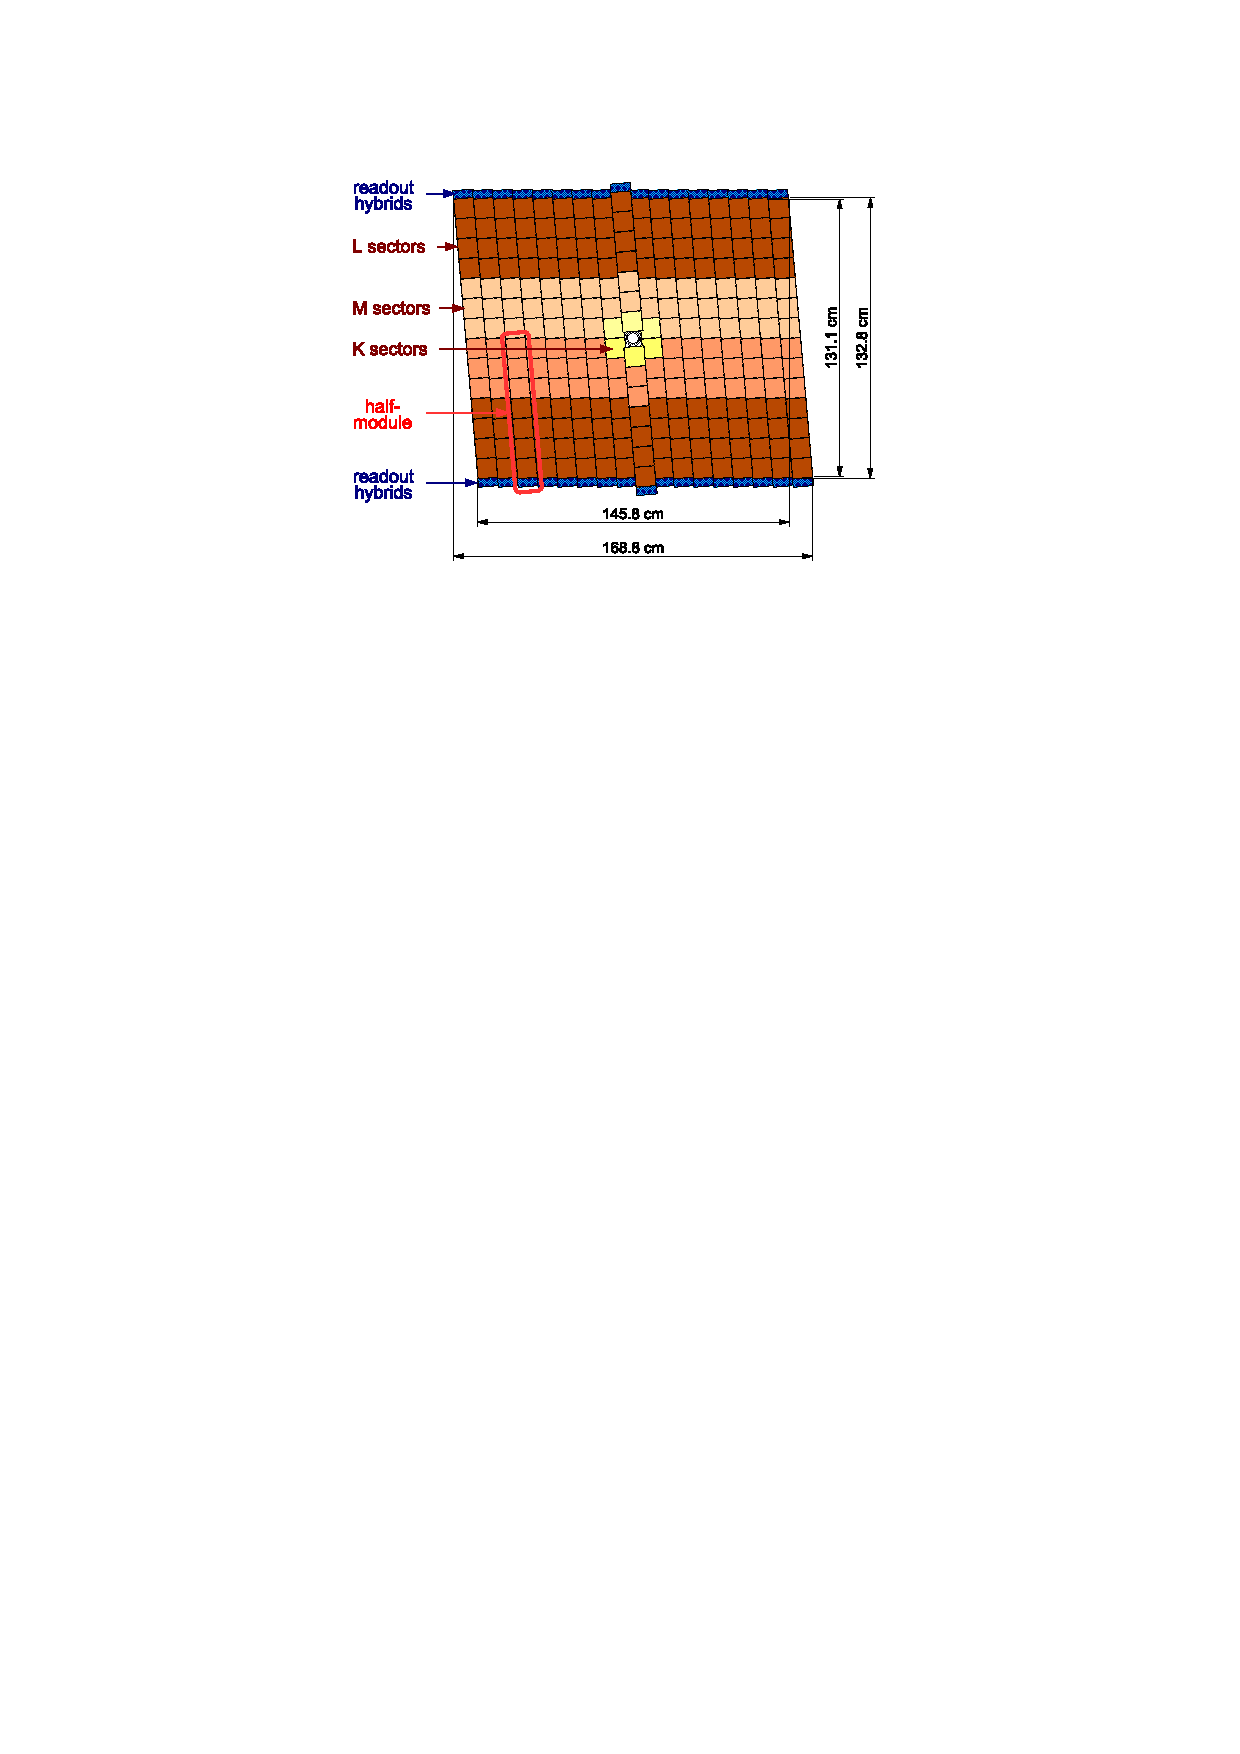
\includegraphics[width=0.6\textwidth]{figs/Detector/tt_layout.pdf}
    \caption{Schematic of the \ttracker sub-detector, from Ref.~\cite{Alves:2008zz}.}
    \label{fig:Dec_tt_layout}   
\end{figure}
%%%%%%%%%%%%%%%%%%%%%%%%%%%%%%%%%%%%%%%%%%%%%%%%%%%%%%%%%%

The \emph{half-modules} are arranged to prevent any gaps in the instrumentation. The adjacent \emph{half-modules} are offset by 1\cm along the beam axis, allowing the modules to overlap by a few millimetres in the $x$-axis. 


{\color{Red}
\begin{itemize}
\item performance
\end{itemize}
}


\subsubsection{Inner Tracker}

The \intr is the second silicon detector making up the \st. It is located after the dipole magnet in three tracking stations. As the name implies, it covers only the inner region of the acceptance, measuring 140\cm wide and 40\cm tall. The rest of the area is covered by the much larger Outer Tracker. Similar to the \ttracker, the \intr is made up of four layers positioned at slight angles to one another. However, as shown in Fig.~\ref{fig:Dec_lhcb_Schematic}, there are three separate \intr stations, each containing four layers.
These stations are constructed as of four boxes distributed around the beam-pipe in a cross shape, as shown in Fig.~\ref{fig:Dec_it_layout}. 

%%%%%%%%%%%%%%%%%%%%%%%%%%%%%%%%%%%%%%%%%%%%%%%%%%%%%%%%%%
\begin{figure}[!h]
    \centering
    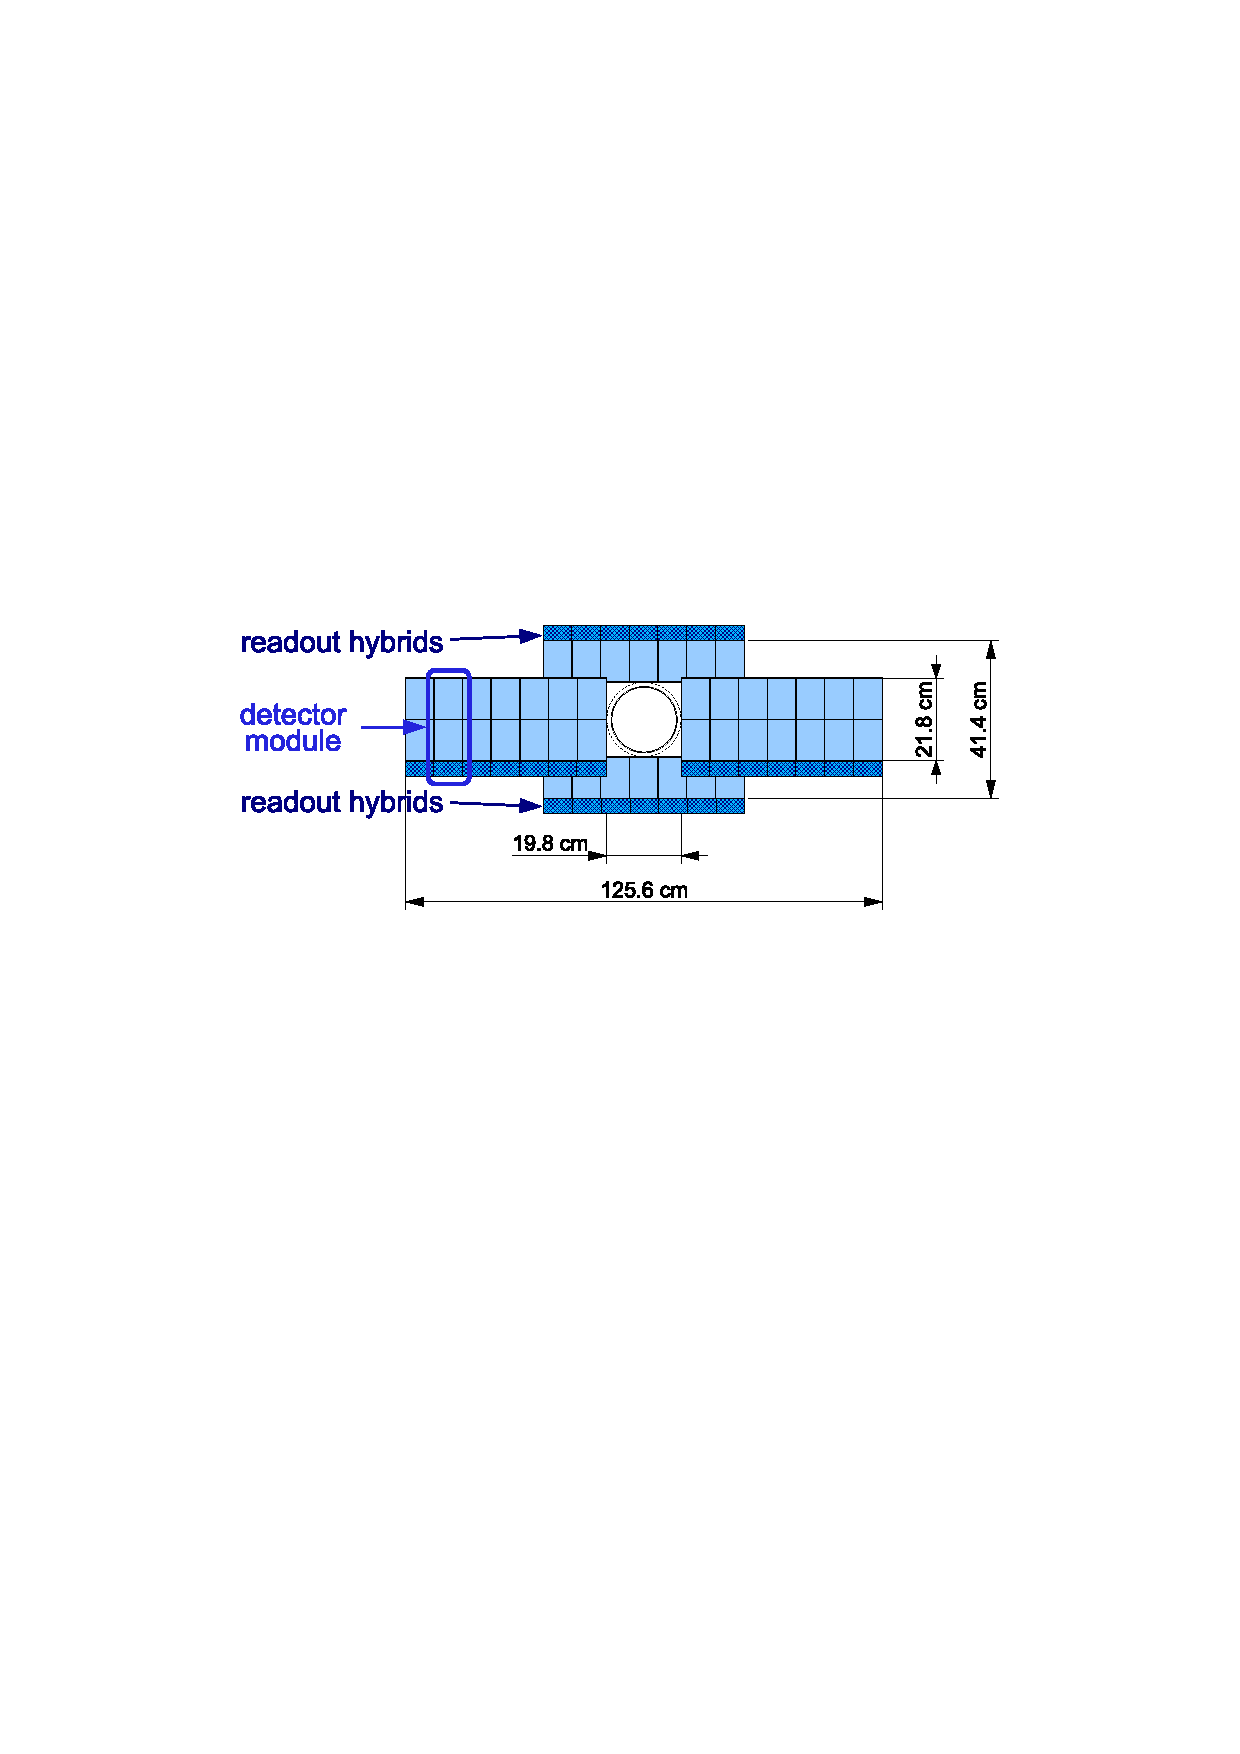
\includegraphics[width=0.6\textwidth]{figs/Detector/it_layout.pdf}
    \caption{Schematic of the \intr sub-detector, from Ref.~\cite{Alves:2008zz}.}
    \label{fig:Dec_it_layout}   
\end{figure}
%%%%%%%%%%%%%%%%%%%%%%%%%%%%%%%%%%%%%%%%%%%%%%%%%%%%%%%%%%

The detector modules consist of either one or two silicon sensors and a readout chip. These are also offset along the beam axis to allow the modules to overlap slightly in the $x$-axis.



\subsection{Outer Tracker}

In contrast to the the silicon-based sub-detectors already described, the Outer Tracker (\ot) is a straw tube tracker filled with a gaseous mixture of argon, carbon dioxide and oxygen. The 4.9\mm diameter straws are 2.4\m in length and arranged in double layers as shown in Fig.~\ref{fig:Dec_ot_schematic}. As with the \intr, the \ot is split into three stations. Each of these stations similarly has four layers arranged at angles to one another $(0\degrees,-5\degrees,+5\degrees,0\degrees)$. The arrangement of the stations and layers are also shown in Fig.~\ref{fig:Dec_ot_schematic}. The inner region occupied by the \intr is visible.
 
%%%%%%%%%%%%%%%%%%%%%%%%%%%%%%%%%%%%%%%%%%%%%%%%%%%%%%%%%%
\begin{figure}[!h]
    \centering
    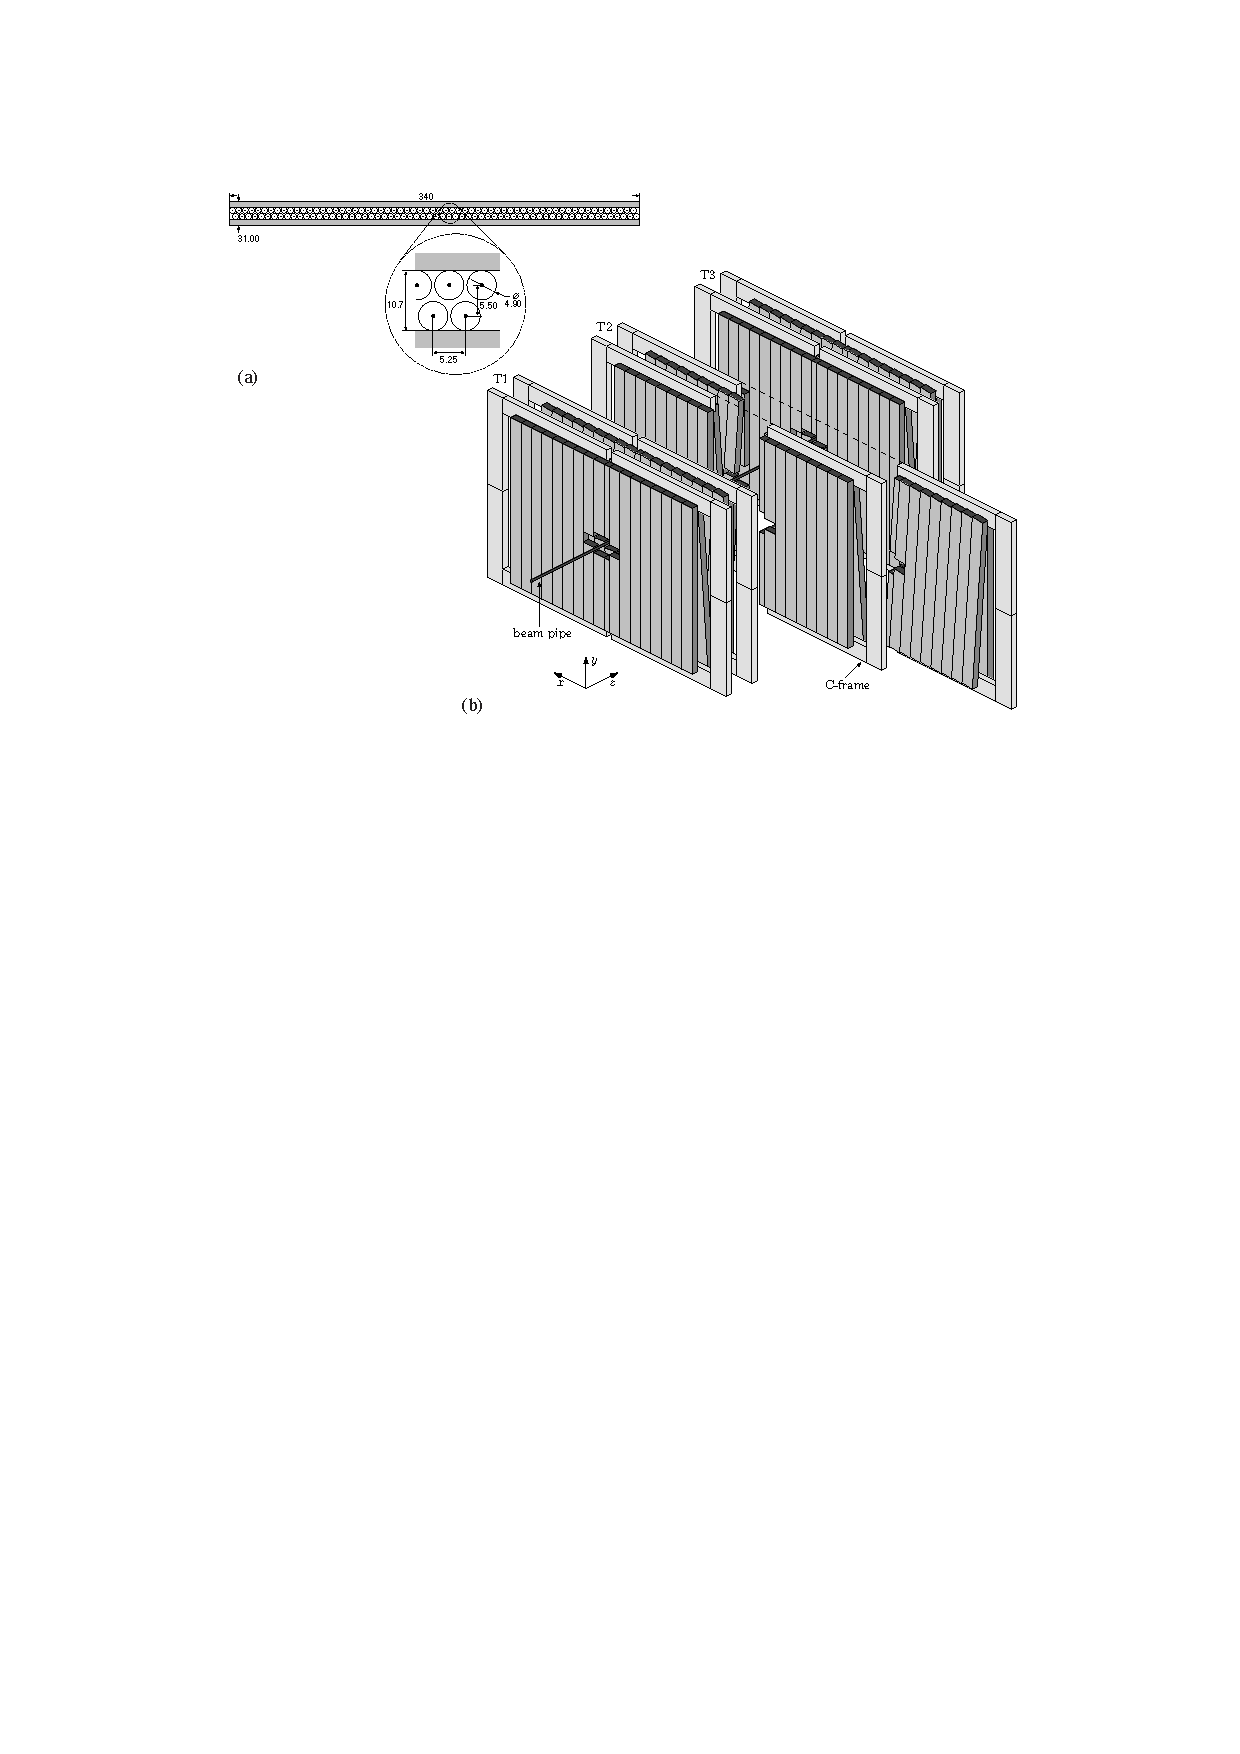
\includegraphics[width=0.8\textwidth]{figs/Detector/ot_layout.pdf}
    \caption{Schematic of the \ot sub-detector, from Ref.~\cite{LHCb-DP-2013-003}.}
    \label{fig:Dec_ot_schematic}   
\end{figure}
%%%%%%%%%%%%%%%%%%%%%%%%%%%%%%%%%%%%%%%%%%%%%%%%%%%%%%%%%%



\subsection{Ring imaging Cherenkov detectors}

The ring imaging Cherenkov detectors (\rich) provide essential information about the particle identification of tracks, allowing different species to be distinguished. This means that kaons and protons can be distinguished from the abundant pions tracks in a typical event. Two \rich sub-detectors are present, each optimised for particles with different momentums. The first, \richone, is located between the \velo and \ttracker, before the particles have passed through the magnetic field. This provides discrimination primarily for low momentum tracks between 1--60\gevc. A second sub-detector, \richtwo, is located between the \intr and \ot tracking stations and calorimeters, after the particles have travelled through the magnetic field. This caters for the higher momentum particles in the range 15--100\gevc. 


{\color{Red}
\begin{itemize}
\item rich principle 
\item mirrors
\item HPDs
\item pattern recognition 
\end{itemize}
}

%%%%%%%%%%%%%%%%%%%%%%%%%%%%%%%%%%%%%%%%%%%%%%%%%%%%%%%%%%
\begin{figure}[!h]
    \centering
    \begin{subfigure}[t]{0.4\textwidth}
        \centering        
        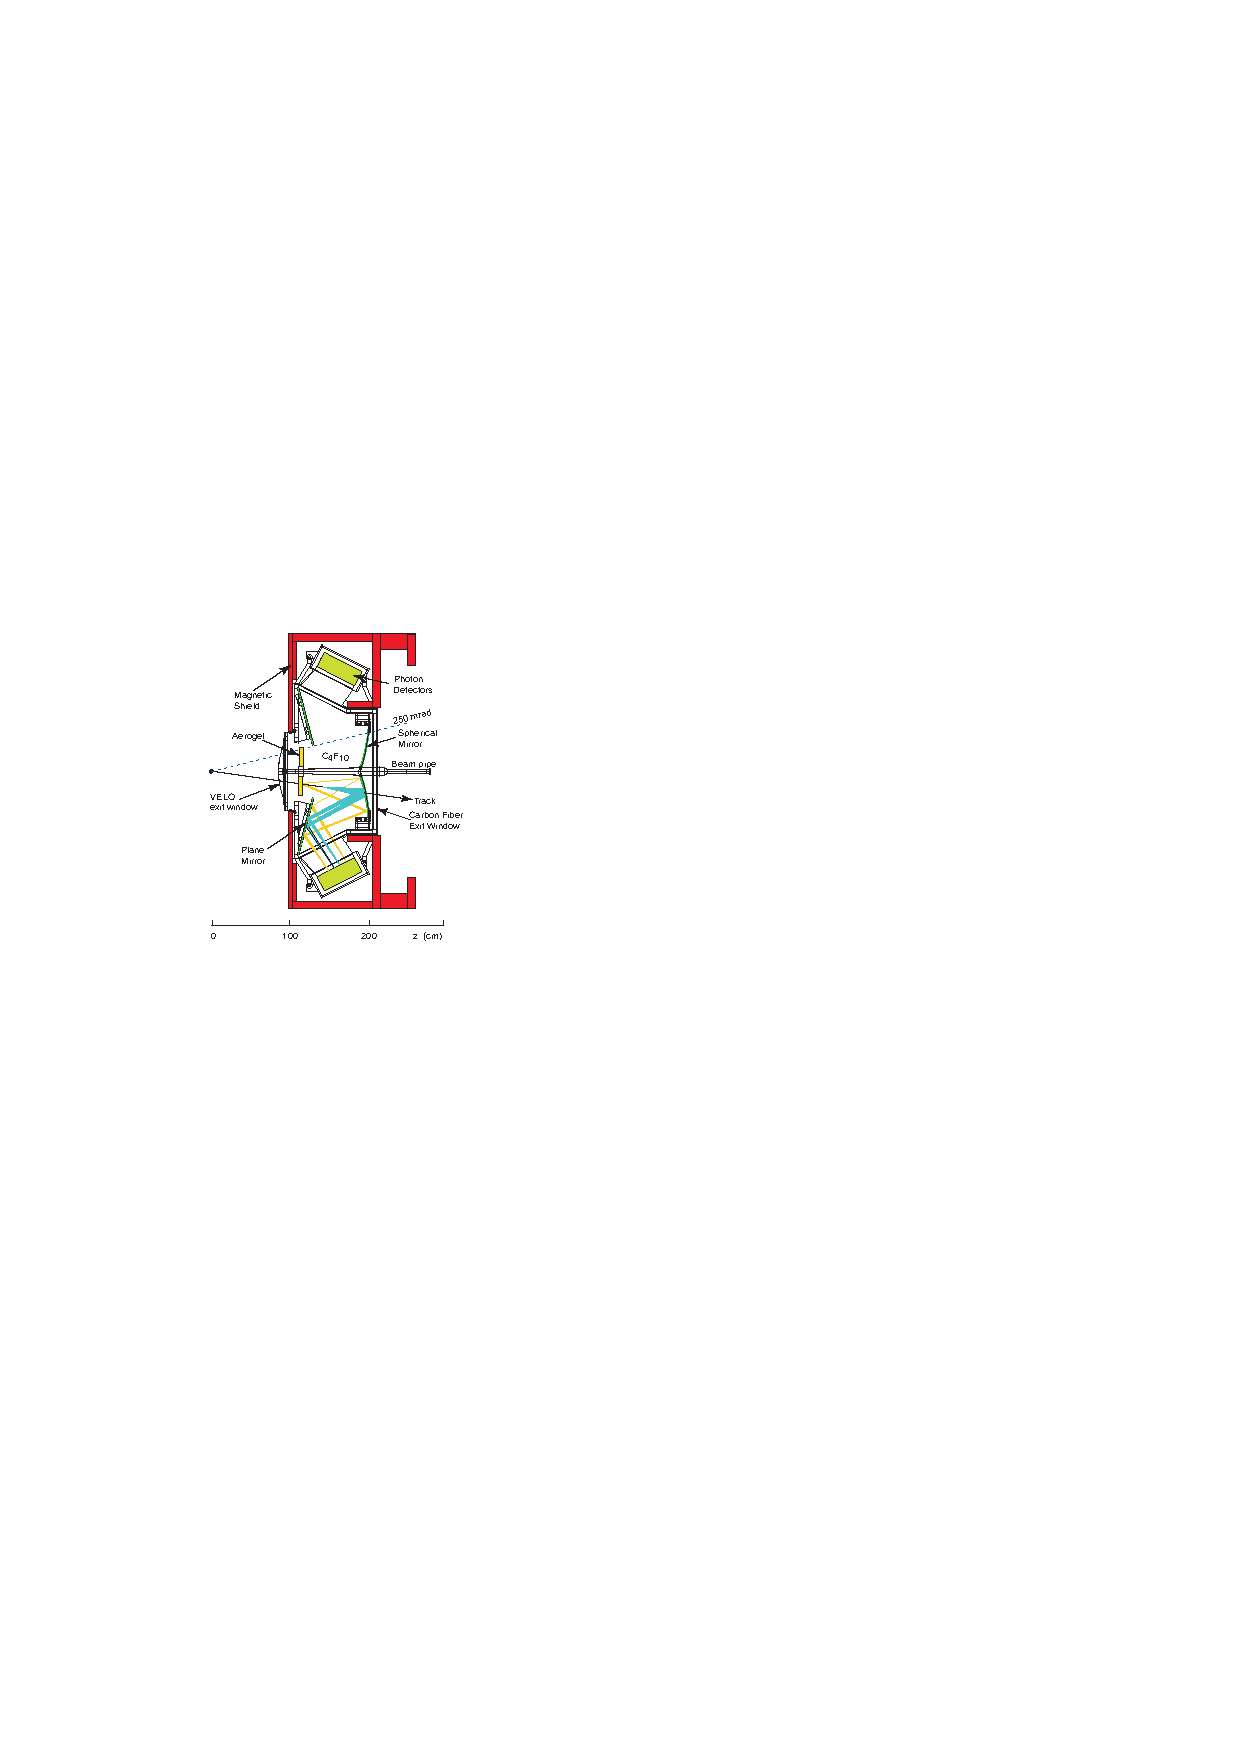
\includegraphics[width=1.0\textwidth]{figs/Detector/richone_layout.pdf}
        \caption{\richone}
    \end{subfigure}
    \begin{subfigure}[t]{0.4\textwidth}
        \centering
        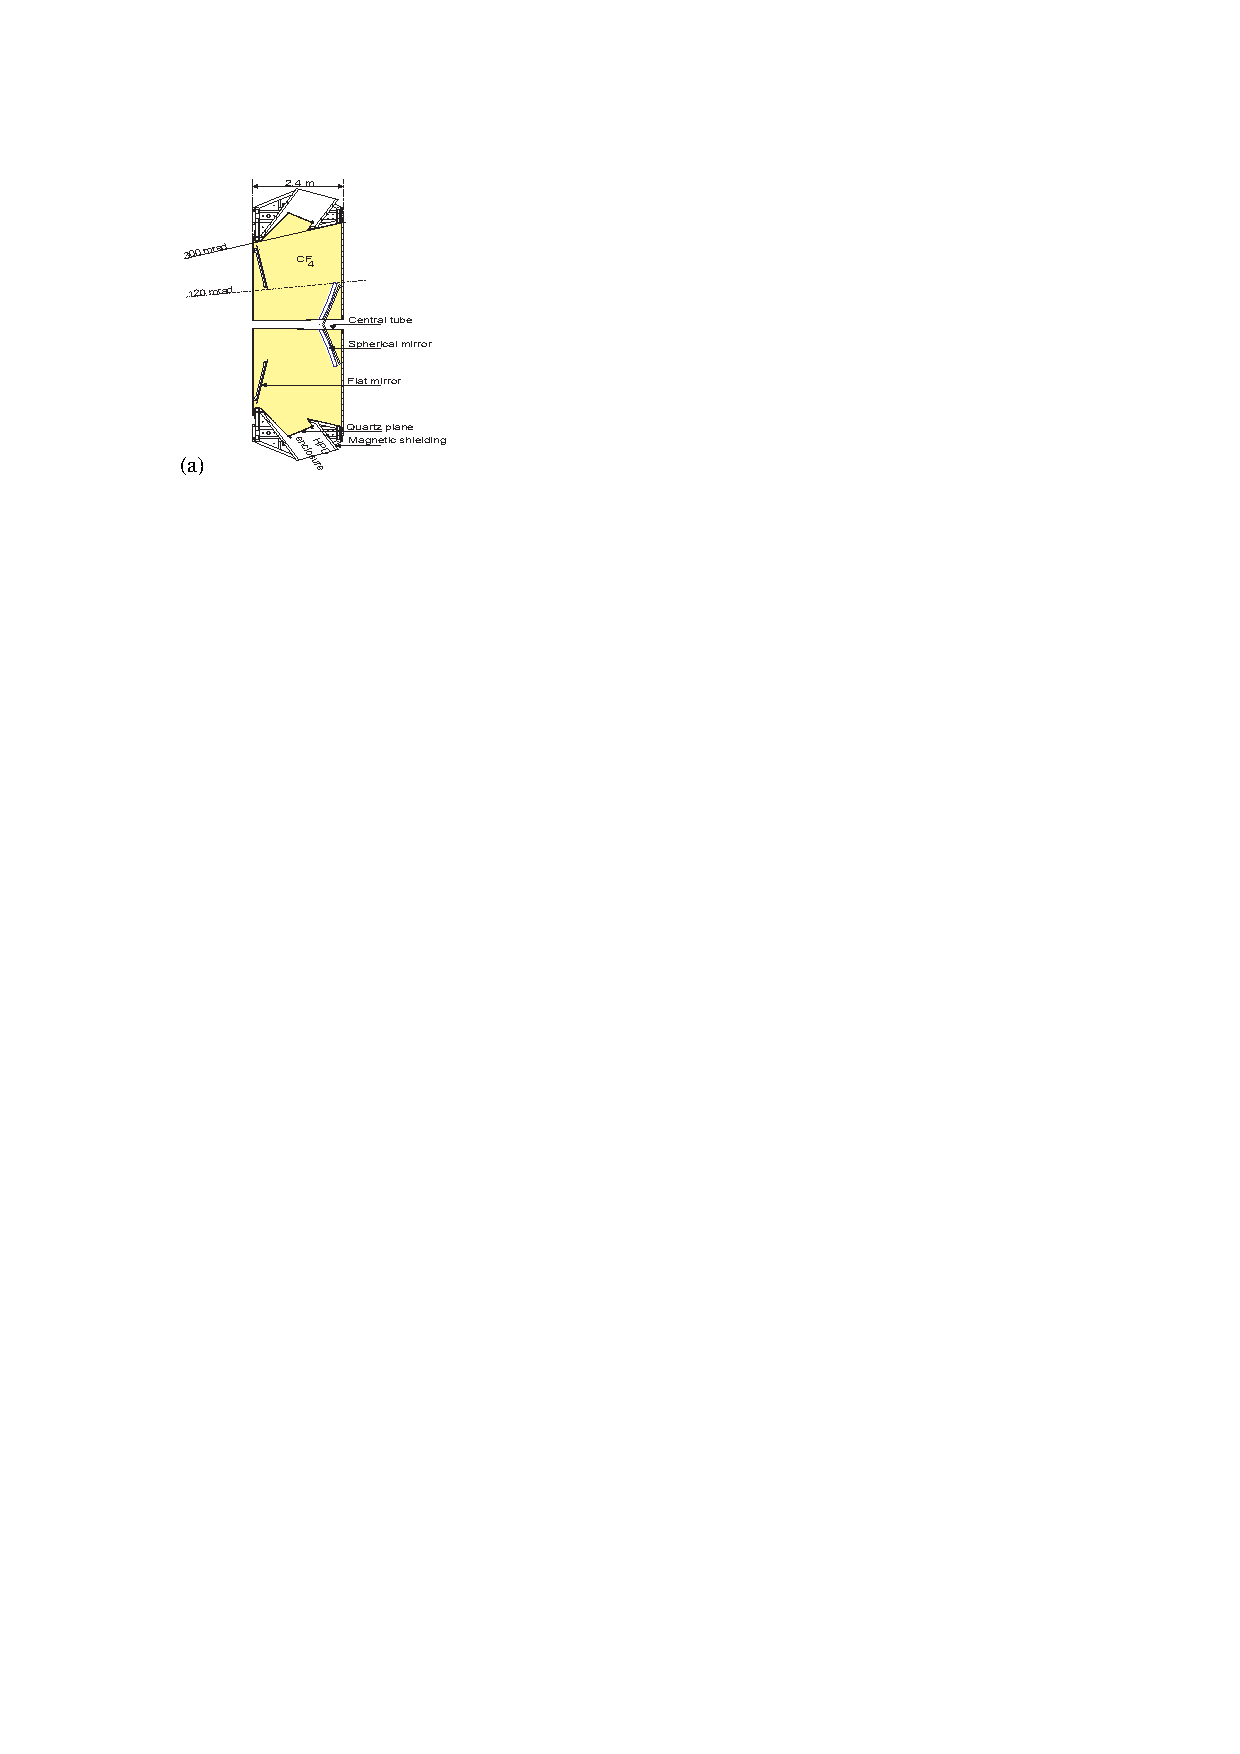
\includegraphics[width=1.0\textwidth]{figs/Detector/richtwo_layout.pdf}
        \caption{\richtwo}
    \end{subfigure}
    \caption{Schematic the \richone and \richtwo sub-detectors from Ref.~\cite{Alves:2008zz}.}

    \label{fig:Dec_rich_layout}   
\end{figure}
%%%%%%%%%%%%%%%%%%%%%%%%%%%%%%%%%%%%%%%%%%%%%%%%%%%%%%%%%%

\subsubsection{\richone}

{\color{Red}
\begin{itemize}
\item radiator and refractive indices 
\item talk about aero gel being removed
\item find some references 
\end{itemize}
}

\subsubsection{\richtwo}

{\color{Red}
\begin{itemize}
\item radiator and refractive indices 
\end{itemize}
}

\subsection{Calorimeters}

The calorimeters measure the energy deposited by particles. This is crucial for the reconstruction of neutral particles that don't leave tracks in the tracking stations. Additionally, the calorimeter plays an important role in the triggering of events.

\subsubsection{Pre-shower detector}
\subsubsection{Electronic Calorimeter}
\subsubsection{Hadron calorimeter}

\subsection{Muon system}

%%%%%%%%%%%%%%%%%%%%%%%%%%%%%%%%%%%%%%%%%%%%%%%%%%%%%%%%%%
\begin{figure}[!h]
    \centering
    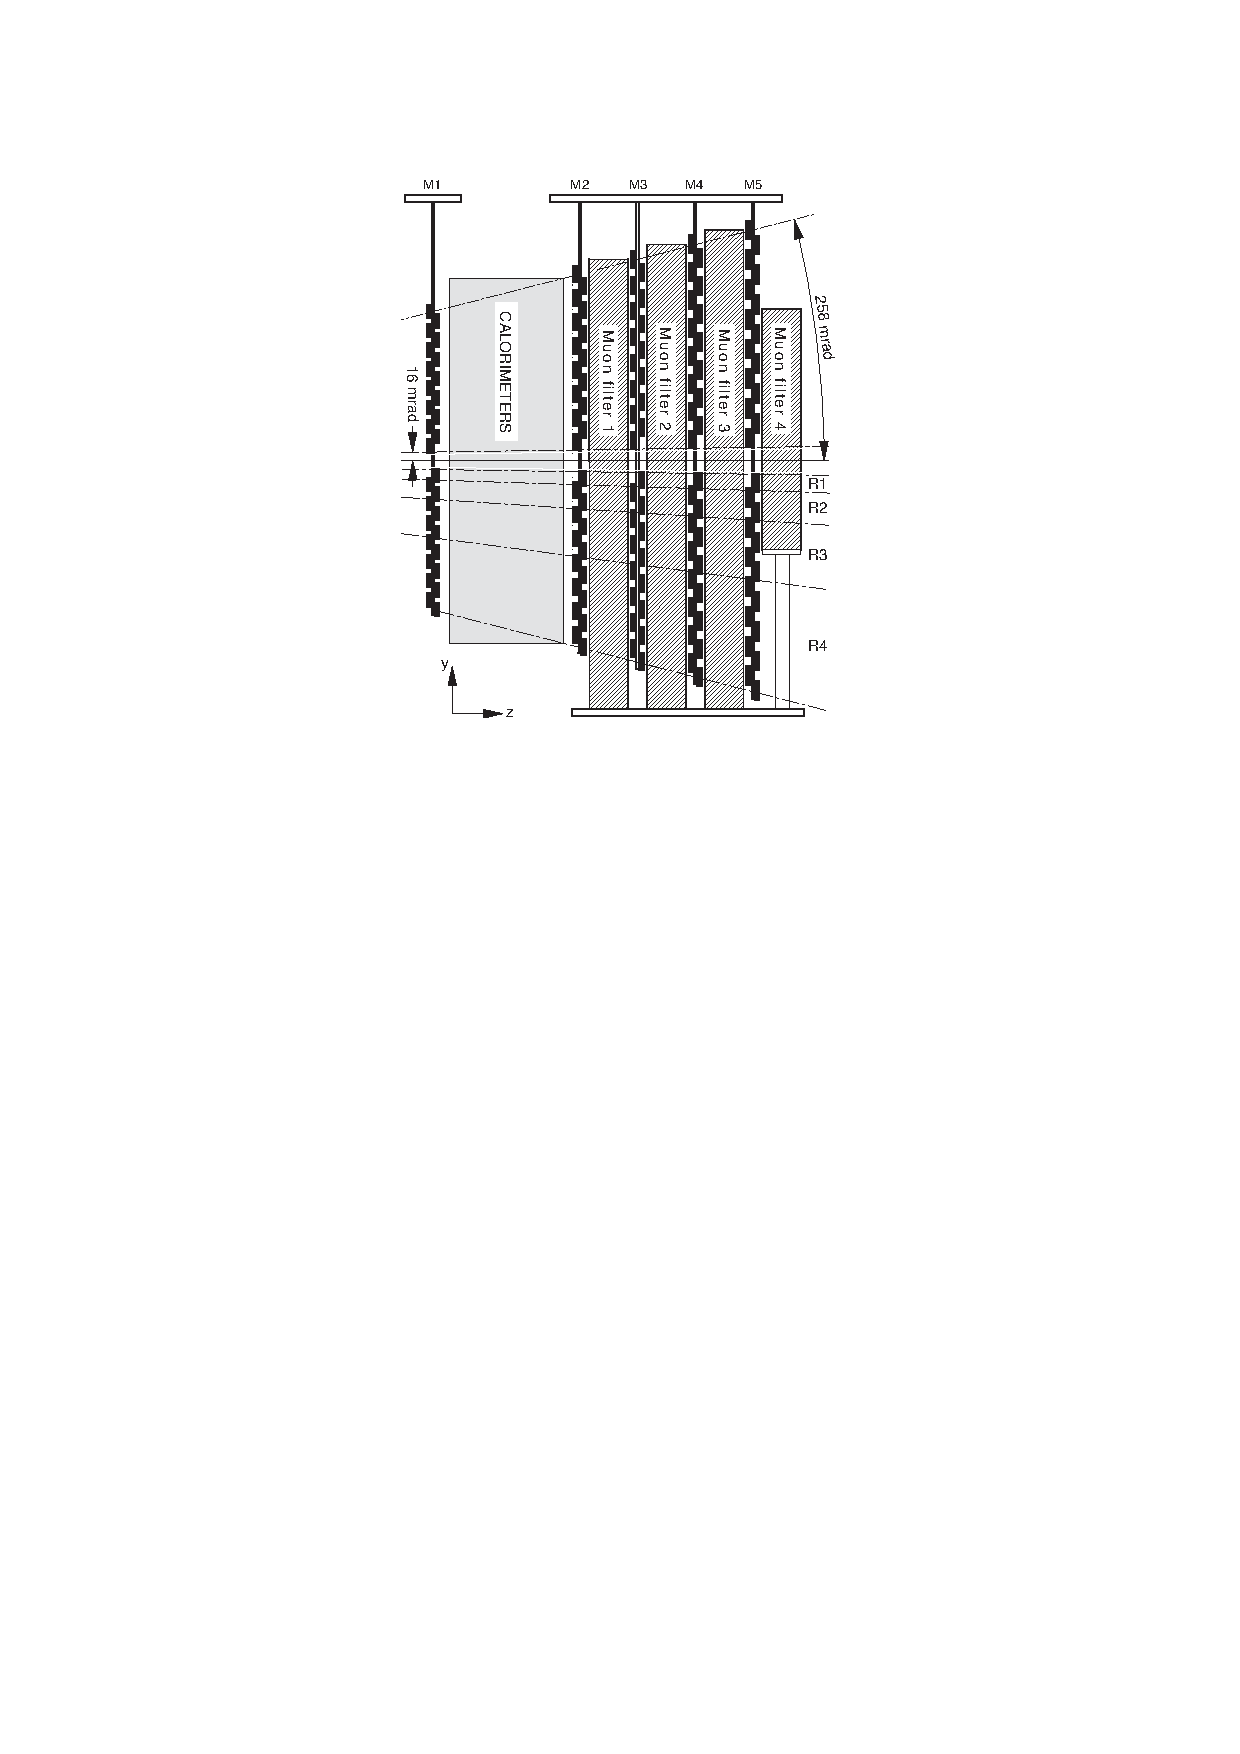
\includegraphics[width=0.4\textwidth]{figs/Detector/muon_layout.pdf}
    \caption{Schematic of the Muon sub-detector, from Ref.~\cite{Alves:2008zz}.}
    \label{fig:Dec_muon_schematic}   
\end{figure}
%%%%%%%%%%%%%%%%%%%%%%%%%%%%%%%%%%%%%%%%%%%%%%%%%%%%%%%%%%

\subsection{Trigger}
\subsubsection{\lone}
\subsubsection{\hltone}
\subsubsection{\hlttwo}

\subsection{Reconstruction}
\subsubsection{Track Reconstruction}


%%%%%%%%%%%%%%%%%%%%%%%%%%%%%%%%%%%%%%%%%%%%%%%%%%%%%%%%%%
\begin{figure}[!h]
    \centering
    \begin{subfigure}[t]{0.4\textwidth}
        \centering
        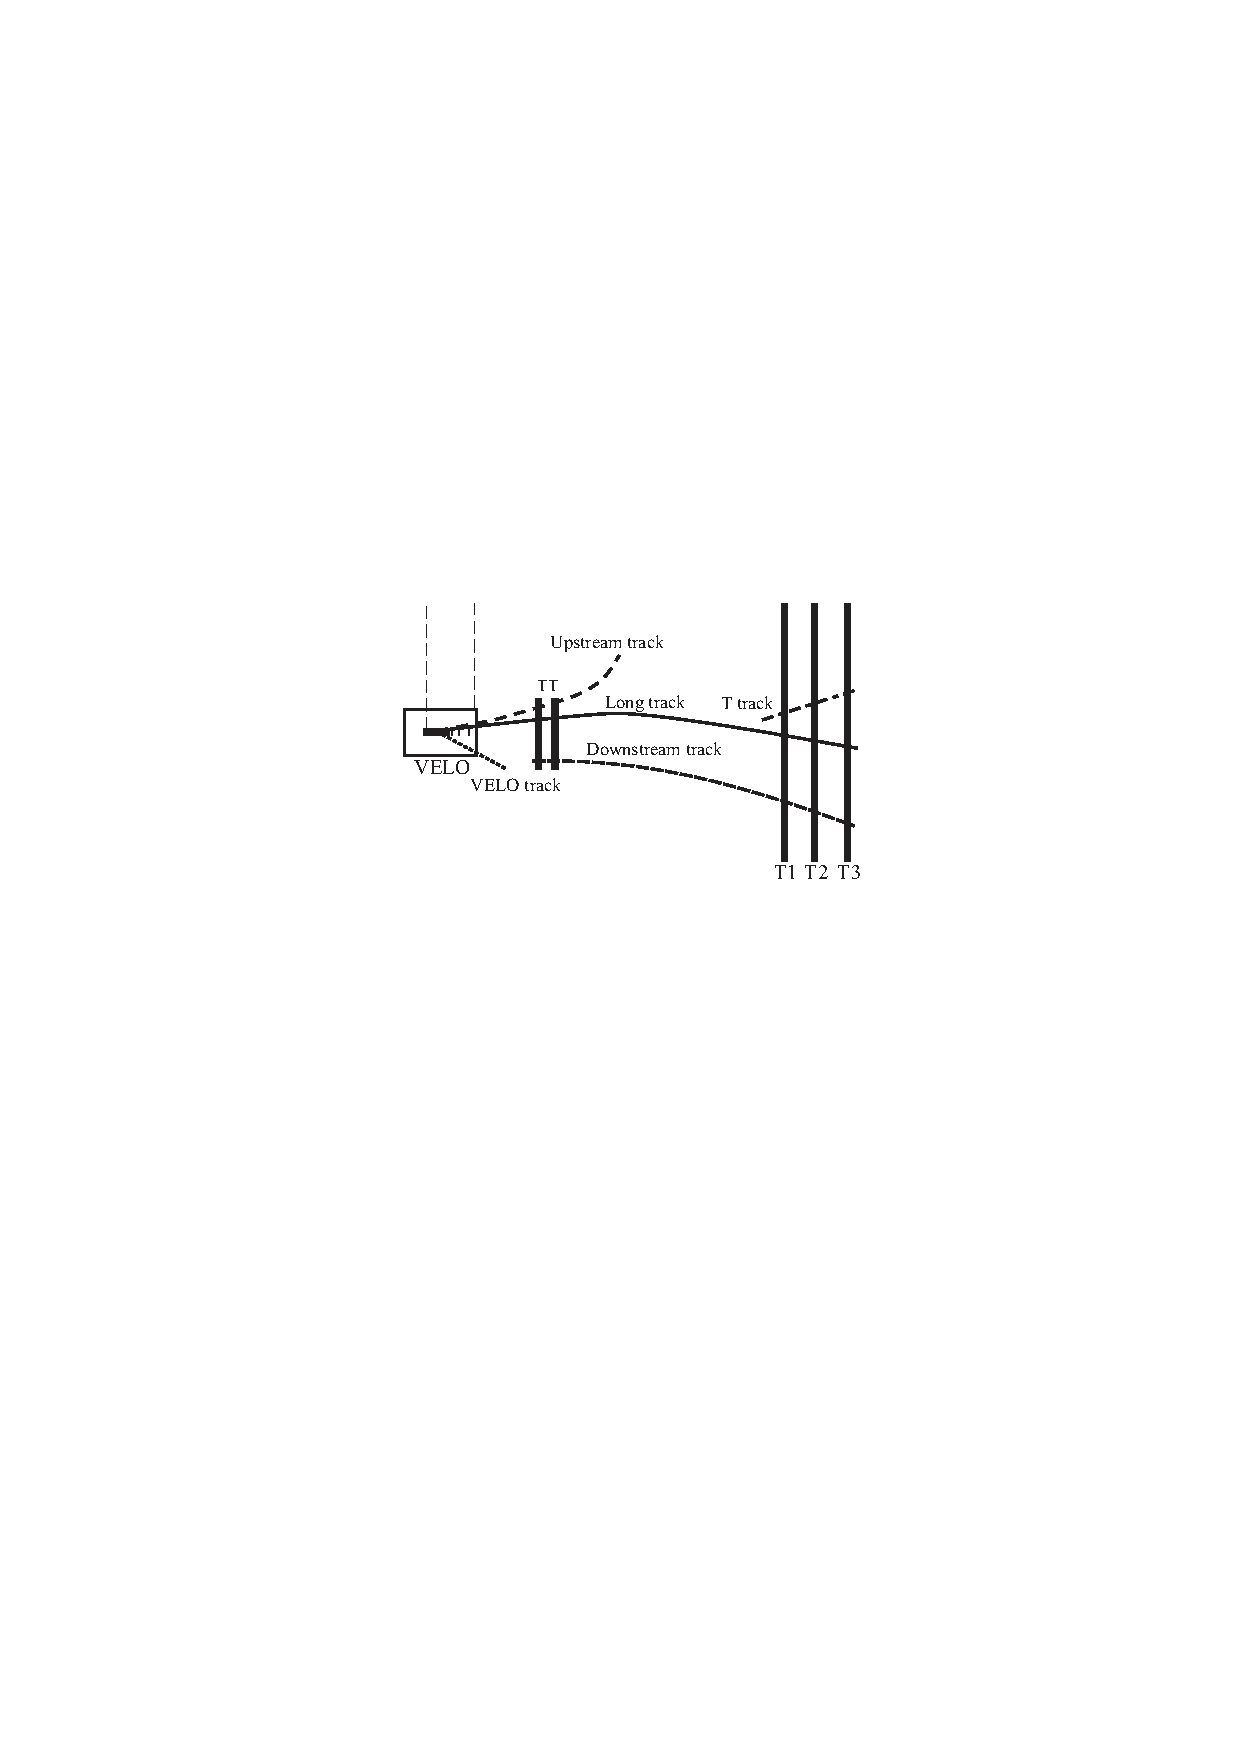
\includegraphics[width=1.0\textwidth]{figs/Detector/reco_track_types.pdf}
    \end{subfigure}
    \begin{subfigure}[t]{0.4\textwidth}
        \centering
        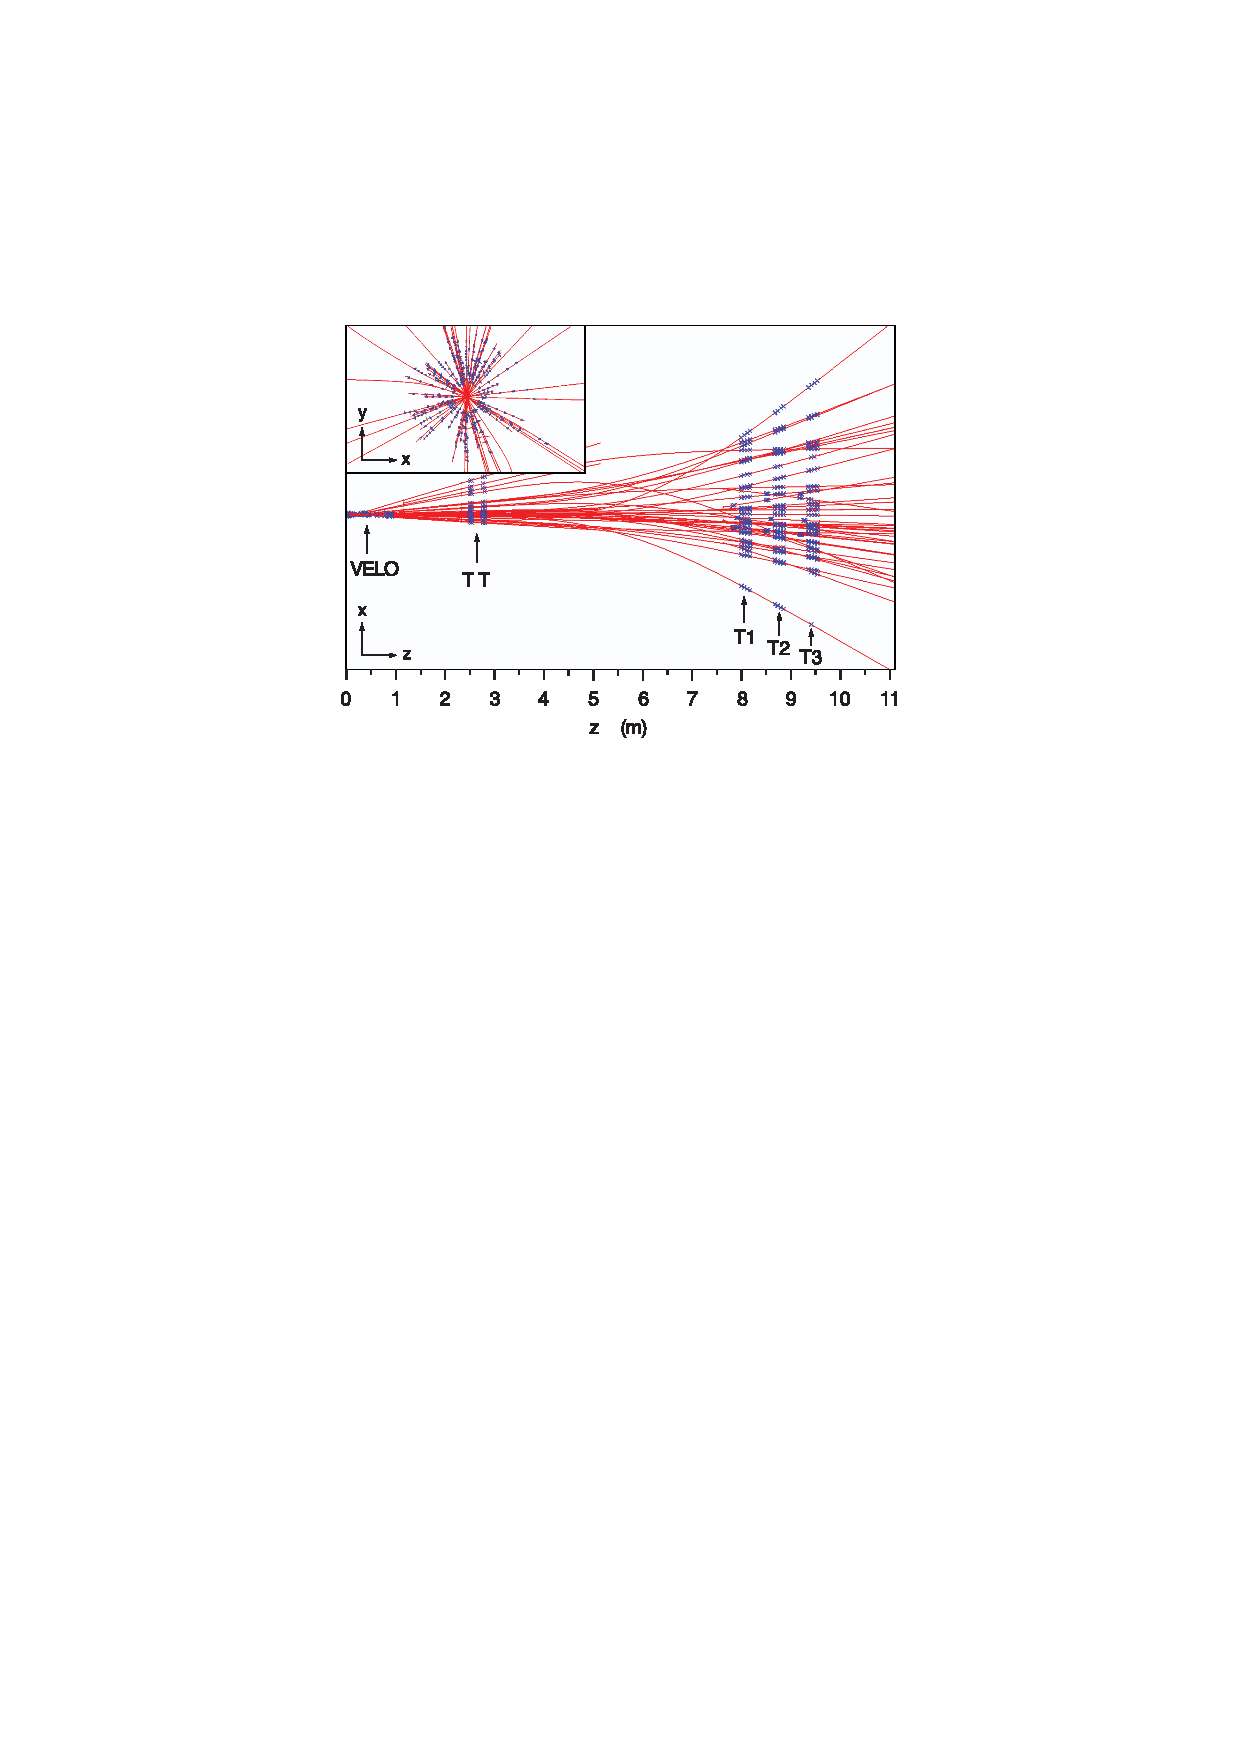
\includegraphics[width=1.0\textwidth]{figs/Detector/reco_track_reco.pdf}
    \end{subfigure}
    \caption{Diagram of the different track reconstruction types (left) and an illustration of the reconstructed tracks in a typical event from Ref.~\cite{LHCb-DP-2014-002}.}
    \label{fig:Dec_reco_tracks}   
\end{figure}
%%%%%%%%%%%%%%%%%%%%%%%%%%%%%%%%%%%%%%%%%%%%%%%%%%%%%%%%%%

\section{VELO resolution and luminosity determination}
\chapter{Event selection} 
\label{ch:selection}

\minitoc

In this chapter the procedures developed to reconstruct and select \decay{\Bp}{\Dsp\phiz} and \decay{\Bp}{\Dsp\Kp\Km} candidates are described. 
In both cases the branching fractions are measured relative to the normalisation channel \decay{\Bp}{\Dsp\Dzb}.
The corresponding selection for the normalisation channel \decay{\Bp}{\Dsp\Dzb} is also described.  


\section{Data samples and Simulations}



\subsection{Data samples}
\label{sec:data}

The searches for \decay{\Bp}{\Dsp\phiz} and \decay{\Bp}{\Dsp\Kp\Km} decays are performed using a combined data sample comprising of the entire Run I data set and a part of the Run II data set, namely the years 2015 and 2016.
The total integrated luminosity obtained for each year is listed in Table~\ref{tab:lumi}, along with the corresponding centre-of-mass energies. 

\begin{table}[h]
   \centering
      \begin{tabular}{ccc}
         \hline
         Year                    & Integrated luminosity (\invfb)  & $\sqrt{s}$ (\tev) \\ 
         \hline
         2011                    & 1.0  &  7 \\
         2012                    & 2.0  &  8 \\
         2015                    & 0.3  & 13 \\
         2016                    & 1.5  & 13 \\
         \hline
      \end{tabular}
   
   \caption{The integrated luminosities obtained during the different data taking periods used in this analysis and the corresponding centre-of-mass energies ($\sqrt{s}$).}
   \label{tab:lumi}
\end{table}

\subsection{Simulation samples}
\label{sec:mc}

Many aspects of the searches for \decay{\Bp}{\Dsp\phiz} and \decay{\Bp}{\Dsp\Kp\Km} decays requires input from simulation samples. This includes the relative selection efficiencies of the signal and normalisation channels and the determination of the invariant mass distributions of the candidates.
The samples are generated separately for each of the running periods listed in Table~\ref{tab:lumi} and for both polarities of the \lhcb dipole magnet. The simulation samples for \decay{\Bp}{\Dsp\phiz} and \decay{\Bp}{\Dsp\Dzb} decays are generated assuming they proceed via pseudo-two-body decays. In contrast, the phase-space dependence of \decay{\Bp}{\Dsp\Kp\Km} decays must be considered when generating these simulations. Samples are generating assuming a flat distribution across the phase-space. 
Additionally, simulations samples are required for many of the background processes considered in the analyses. These are generated using the same framework and processed using the same reconstruction as the signal modes.


In the simulations, $pp$ collisions are generated using \pythia~\cite{Sjostrand:2007gs,Sjostrand:2006za} with a specific \lhcb configuration~\cite{LHCb-PROC-2010-056}.  Decays of hadronic particles are described by \evtgen~\cite{Lange:2001uf}, in which final-state radiation is generated using \photos~\cite{Golonka:2005pn}. The interaction of the generated particles with the detector, and its response, are implemented using the \geant toolkit~\cite{Allison:2006ve, *Agostinelli:2002hh} as described in Ref.~\cite{LHCb-PROC-2011-006}.


\section{Online selection}
\label{sec:selection_trigger}

The nominal collision frequency at the \lhc is 40\,MHz. In Run II, this corresponded to a peak \Bpm-hadron production rate of around 17\,kHz, assuming a peak luminosity of $\mathcal{L} = 2\times10^{32}\cm^{-2}\,\sec^{-1}$ and \Bpm-hadron production cross-section of $\sigma(\decay{\proton\proton}{\Bpm X}) \sim 87\mub$~\cite{LHCb-PAPER-2017-037}. Of these, only a rate of 156\,Hz correspond to the normalisation channel mode \decay{\Bp}{\Dsp\Dzb}, reduced to 0.04\,Hz when also requiring the \D mesons to decay to the appropriate final states. The selection aims to reduce overall rate of collisions, whilst maximising the signal efficiency. 

The online event selection is performed by the \lhcb trigger, which consists of a hardware stage, based on information from the calorimeter and muon systems, followed by a software stage, which reconstructs the full event, as detailed in Sec.~\ref{sec:Dec_trigger}. 
Trigger decisions are made globally for a given event; either the event is saved or it's discarded. However, for events that are retained more detailed information about the specific interaction that initiated the trigger can be used to help isolate events containing signal candidates. At both hardware and software level there are a number of different triggers that can lead to an event being retained. In hardware this is broadly separated according to the sub-detector that contained the triggering deposit. 
The single-muon and double-muon hardware triggers are initiated by high \pt deposits in the muon system whilst the hadronic trigger is initiated by \hcal clusters. 
%Deposits in the muon chambers or hadronic calorimeter would fire \texttt{L0Muon} or \texttt{L0Hadron} respectively. 
Deposits in the \ecal can trigger the photon or electron hardward trigger, depending on whether the hit was associated with an \spd hit.
%Electromagnetic calorimeter deposits could result in \texttt{L0Electron} or \texttt{L0Photon} firing. 
The \decay{\Bp}{\Dsp\Kp\Km} and \decay{\Bp}{\Dsp}{\phiz} decays are both reconstructed in fully hadronic final states, therefore events retained as a result of the electron, photon or muon triggers are unlikely to have been caused by the signal decays. 

% In addition to specifying which triggers fired, it is possible to use more granular information about the specific hits initiating the trigger to improve the selection of signal candidates. The tracks constituting the reconstructed candidate are matched to the deposits in each sub-detector. 
After the \emph{offline} track reconstruction has been performed, the \Bp meson tracks are matched to the deposits in each triggering sub-detector.
The fraction of the \emph{online} reconstructed trigger candidate hits that are contained within the set of all \emph{offline} \Bp candidate hits are compared and required to be above thresholds that vary between sub-detector systems, as listed in Table~\ref{tab:tosfrac}. This matching determines if the candidate was responsible for the positive trigger decision. The sub-detectors involved in the hardware trigger have lower thresholds than those associated to tracking systems that contribute to the higher level triggers.  

% For a simple trigger candidate (e.g. Track), more than around 70% (depending on the subdetector)
% of the online reconstructed trigger candidate hits need to be contained within the set of all the hits from
% all offline reconstructed signal parts. For a composite candidate, the combination of all individual trigger
% candidates is compared to the set of offline candidates.



%The fraction of the reconstructed objects hits required to match in order for the trigger decision to be associated to that object vary depending on the sub-detector in question, as listed in Table~\ref{tab:tosfrac}.
\begin{table}[h]
   \centering
      \begin{tabular}{cc}
         \hline
         Sub-detector    &  Fraction of matching hits \\
         \hline 
         \hcal          & 1\%    \\ 
         \ecal          & 1\%    \\ 
         Muon           & 0.01\% \\ 
         \ttracker      & 0\%    \\ 
         \intr and \ot  & 70\%   \\ 
         \velo          & 70\%   \\ 
         \hline
      \end{tabular}
   
   \caption{The fraction of \emph{online} hits required to be within the set of all \emph{offline} reconstructed hits for each sub-detector system. The \ttracker and Muon system are essentially not used in this matching. }
   \label{tab:tosfrac}
   %% From: https://gitlab.cern.ch/lhcb/Phys/blob/83e7320119561a4e4996e51a96601f65f1ff5cfe/Phys/TisTosTobbing/src/lib/TisTos.cpp
   %% https://gitlab.cern.ch/lhcb/Phys/blob/2016-patches/Phys/TisTosTobbing/src/lib/TisTos.cpp
\end{table}
Reconstructed objects are classified into categories when considering their relationship to the various decisions made in a given event. 
These categories are,
\begin{description}
\item \textbf{Triggered on Signal:} if the deposited matched to a reconstructed object was sufficient to have initiated a given trigger then this object is said to be \emph{Triggered on Signal} (\texttt{TOS}) with respect to that trigger (Fig.~\ref{fig:TOS}). As such, if the hits that this object caused were removed from the events the trigger would no longer have been initiated.
\item \textbf{Triggered Independently of Signal:} conversely, if the specific trigger fired solely due to other interactions within the same event the object is \emph{Triggered Independently of Signal} (\texttt{TIS}) with respect to that trigger (Fig.~\ref{fig:TIS}). In this case, removal of hits matched to the object would not affect the trigger decision.  It is possible for a candidate to be both \texttt{TIS} and \texttt{TOS} (Fig.~\ref{fig:TOSandTIS}).
\item \textbf{Triggered on Both:} a third category is possible, \emph{Triggered on Both} (\texttt{TOB}), where both the signal object and another object are required to reach the threshold for a positive trigger decision (Fig.~\ref{fig:TOB}). In this situation neither are sufficient to individually initiate the trigger, but removing either one of them would prevent the a positive trigger decision. Events in this category are not considered in this analysis.
\end{description}

%%%%%%%%%%%%%%%%%%%%%%%%%%%%%%%%%%%%%%%%%%%%%%%%%%%%%%%%%%
\begin{figure}[!h]
    \centering
    \begin{subfigure}[t]{0.4\textwidth}
        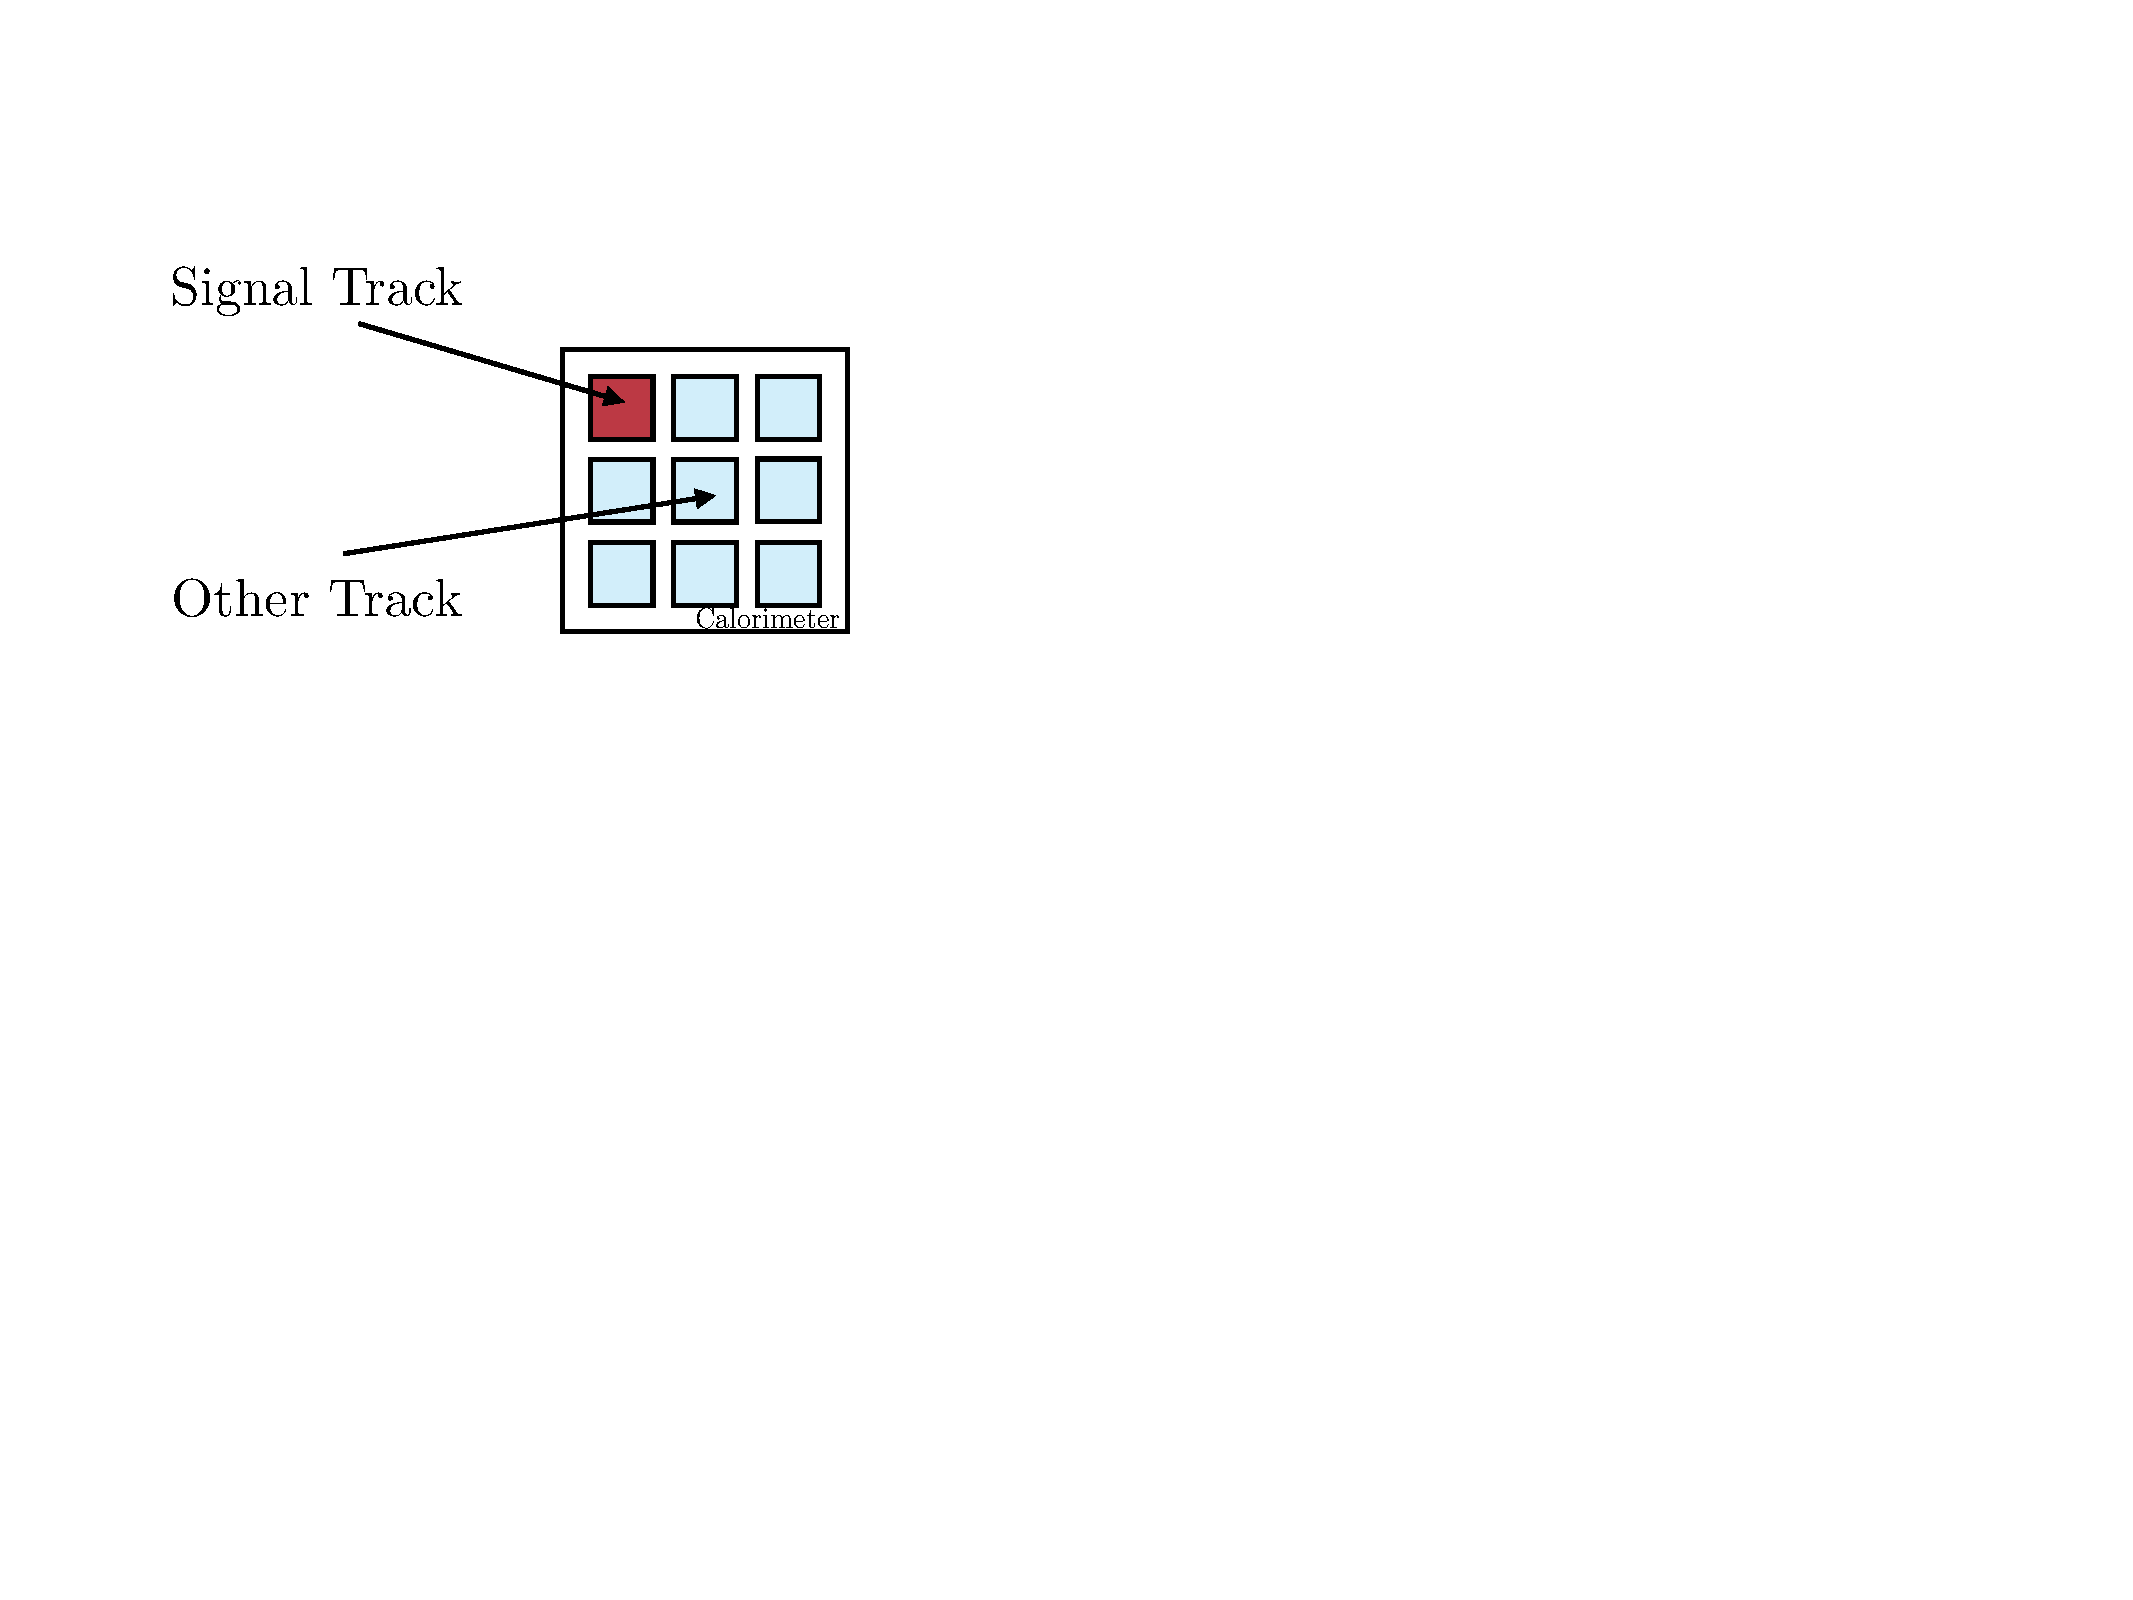
\includegraphics[width=1.0\textwidth]{figs/Selection/Tos.pdf}
        \caption{\texttt{TOS}}
        \label{fig:TOS}
    \end{subfigure}%
    \begin{subfigure}[t]{0.4\textwidth}
        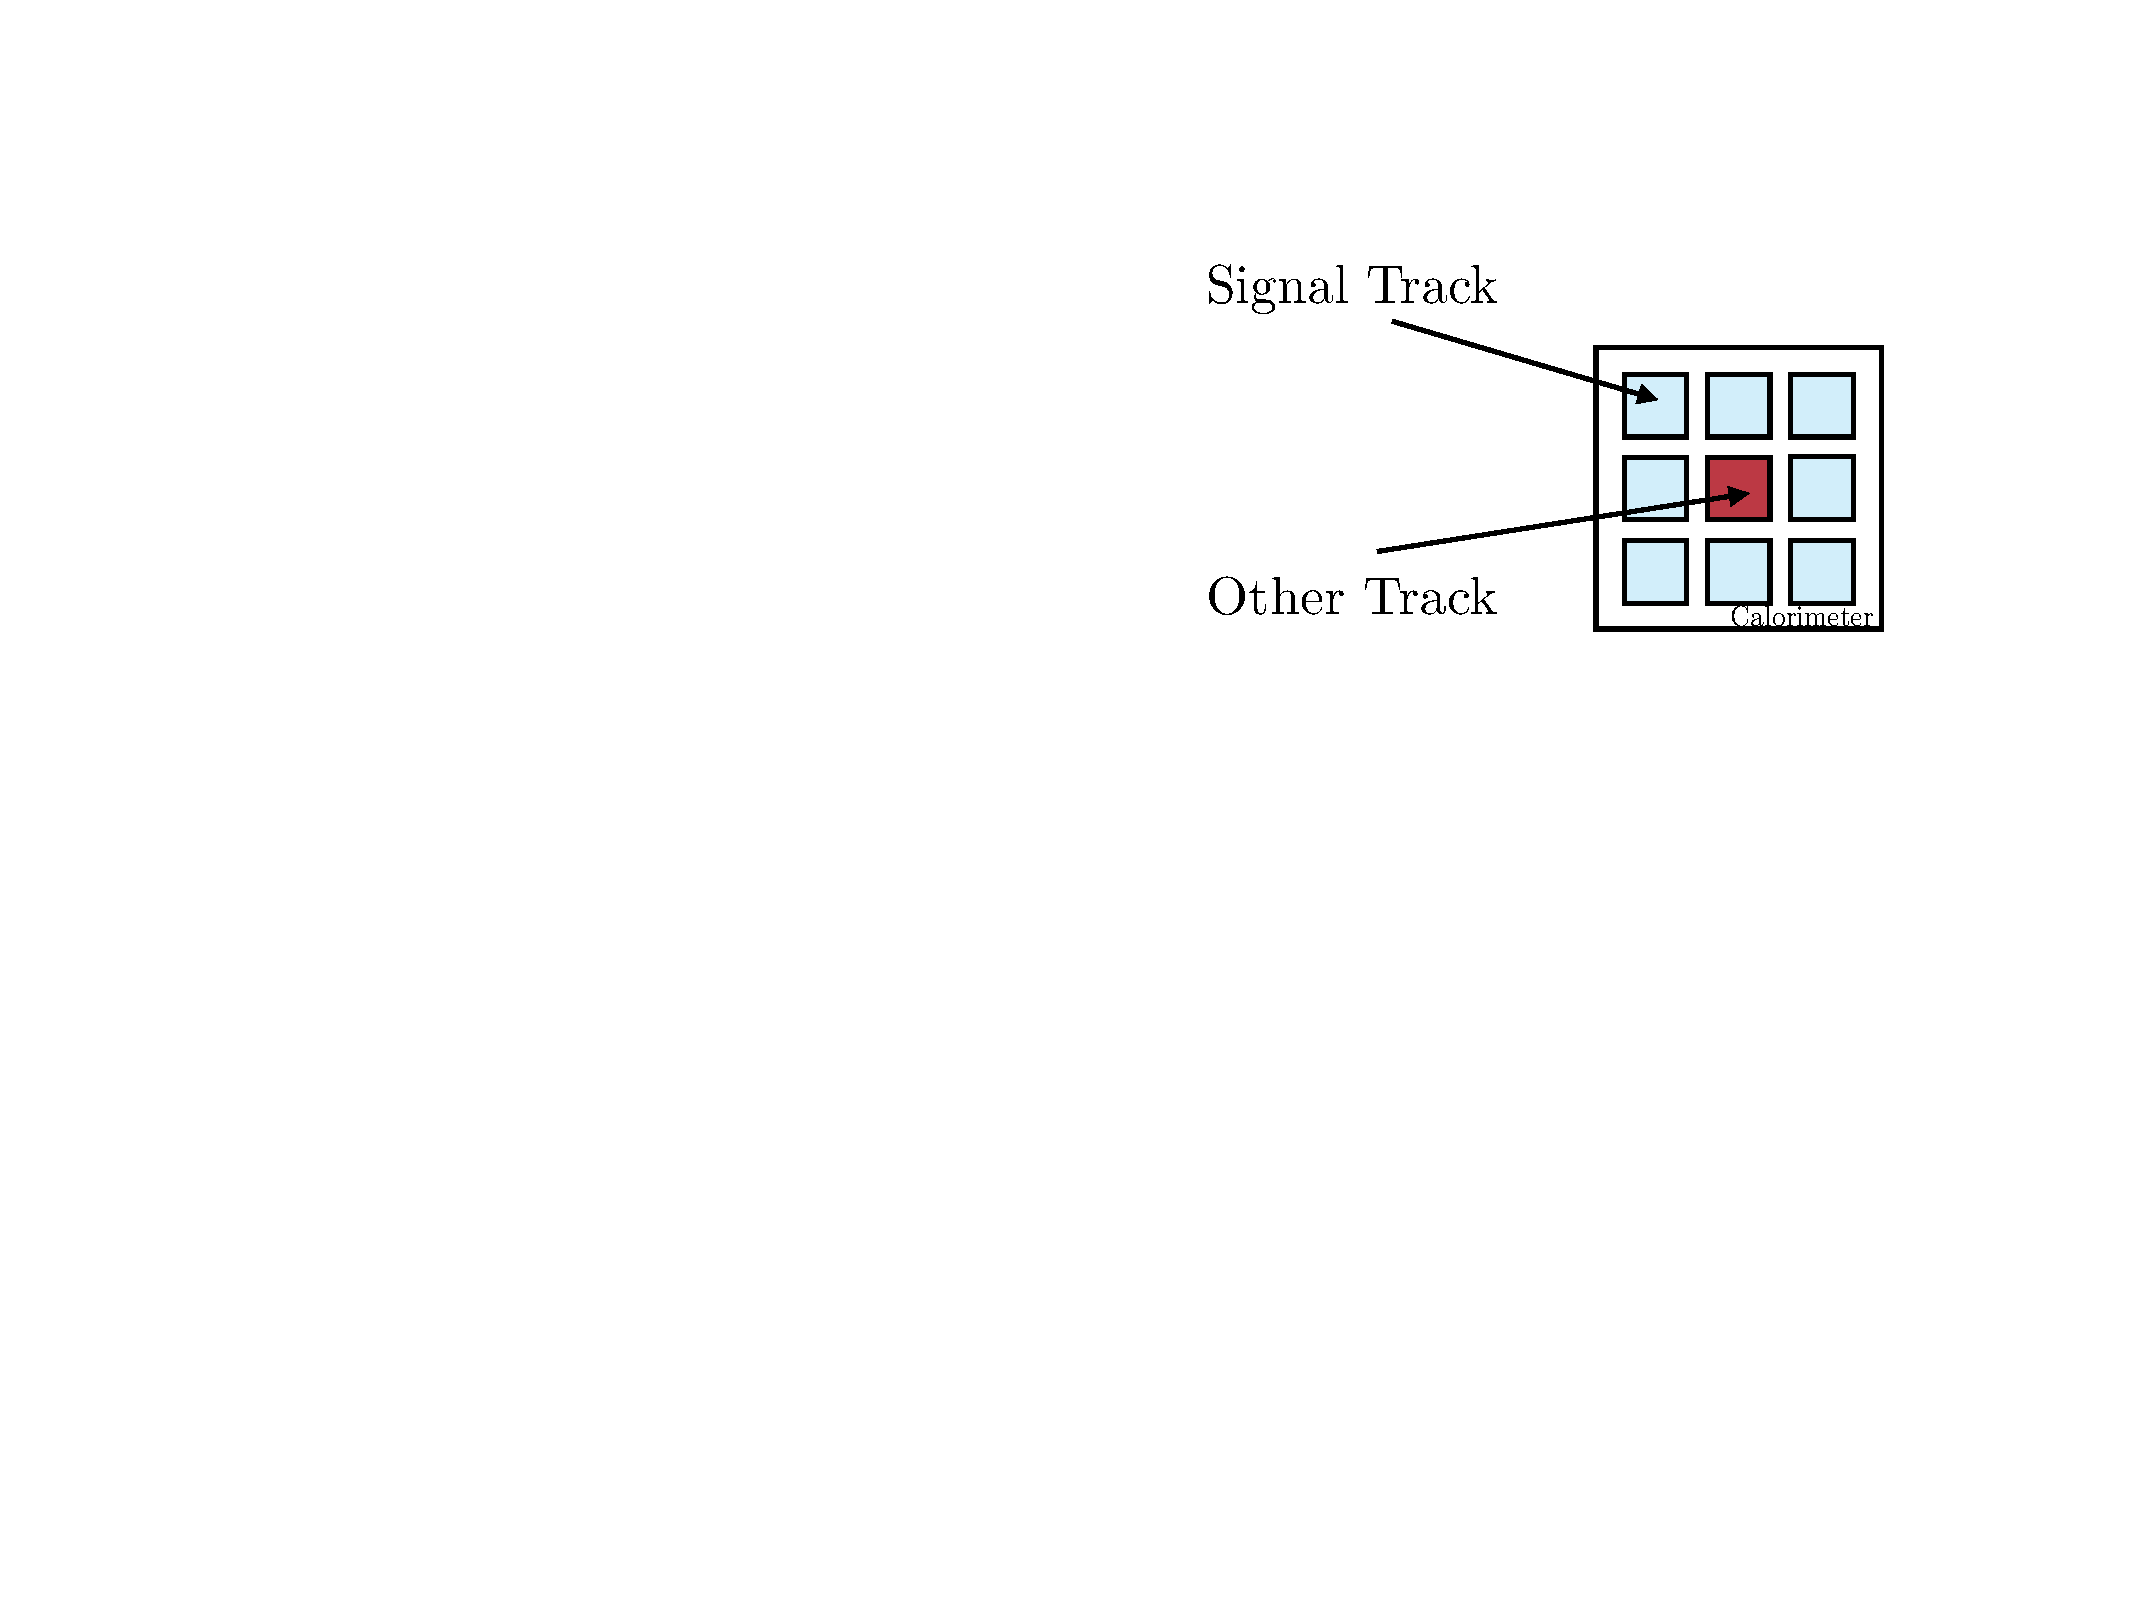
\includegraphics[width=1.0\textwidth]{figs/Selection/Tis.pdf}
        \caption{\texttt{TIS}}
        \label{fig:TIS}
    \end{subfigure}\\
    \begin{subfigure}[t]{0.4\textwidth}
        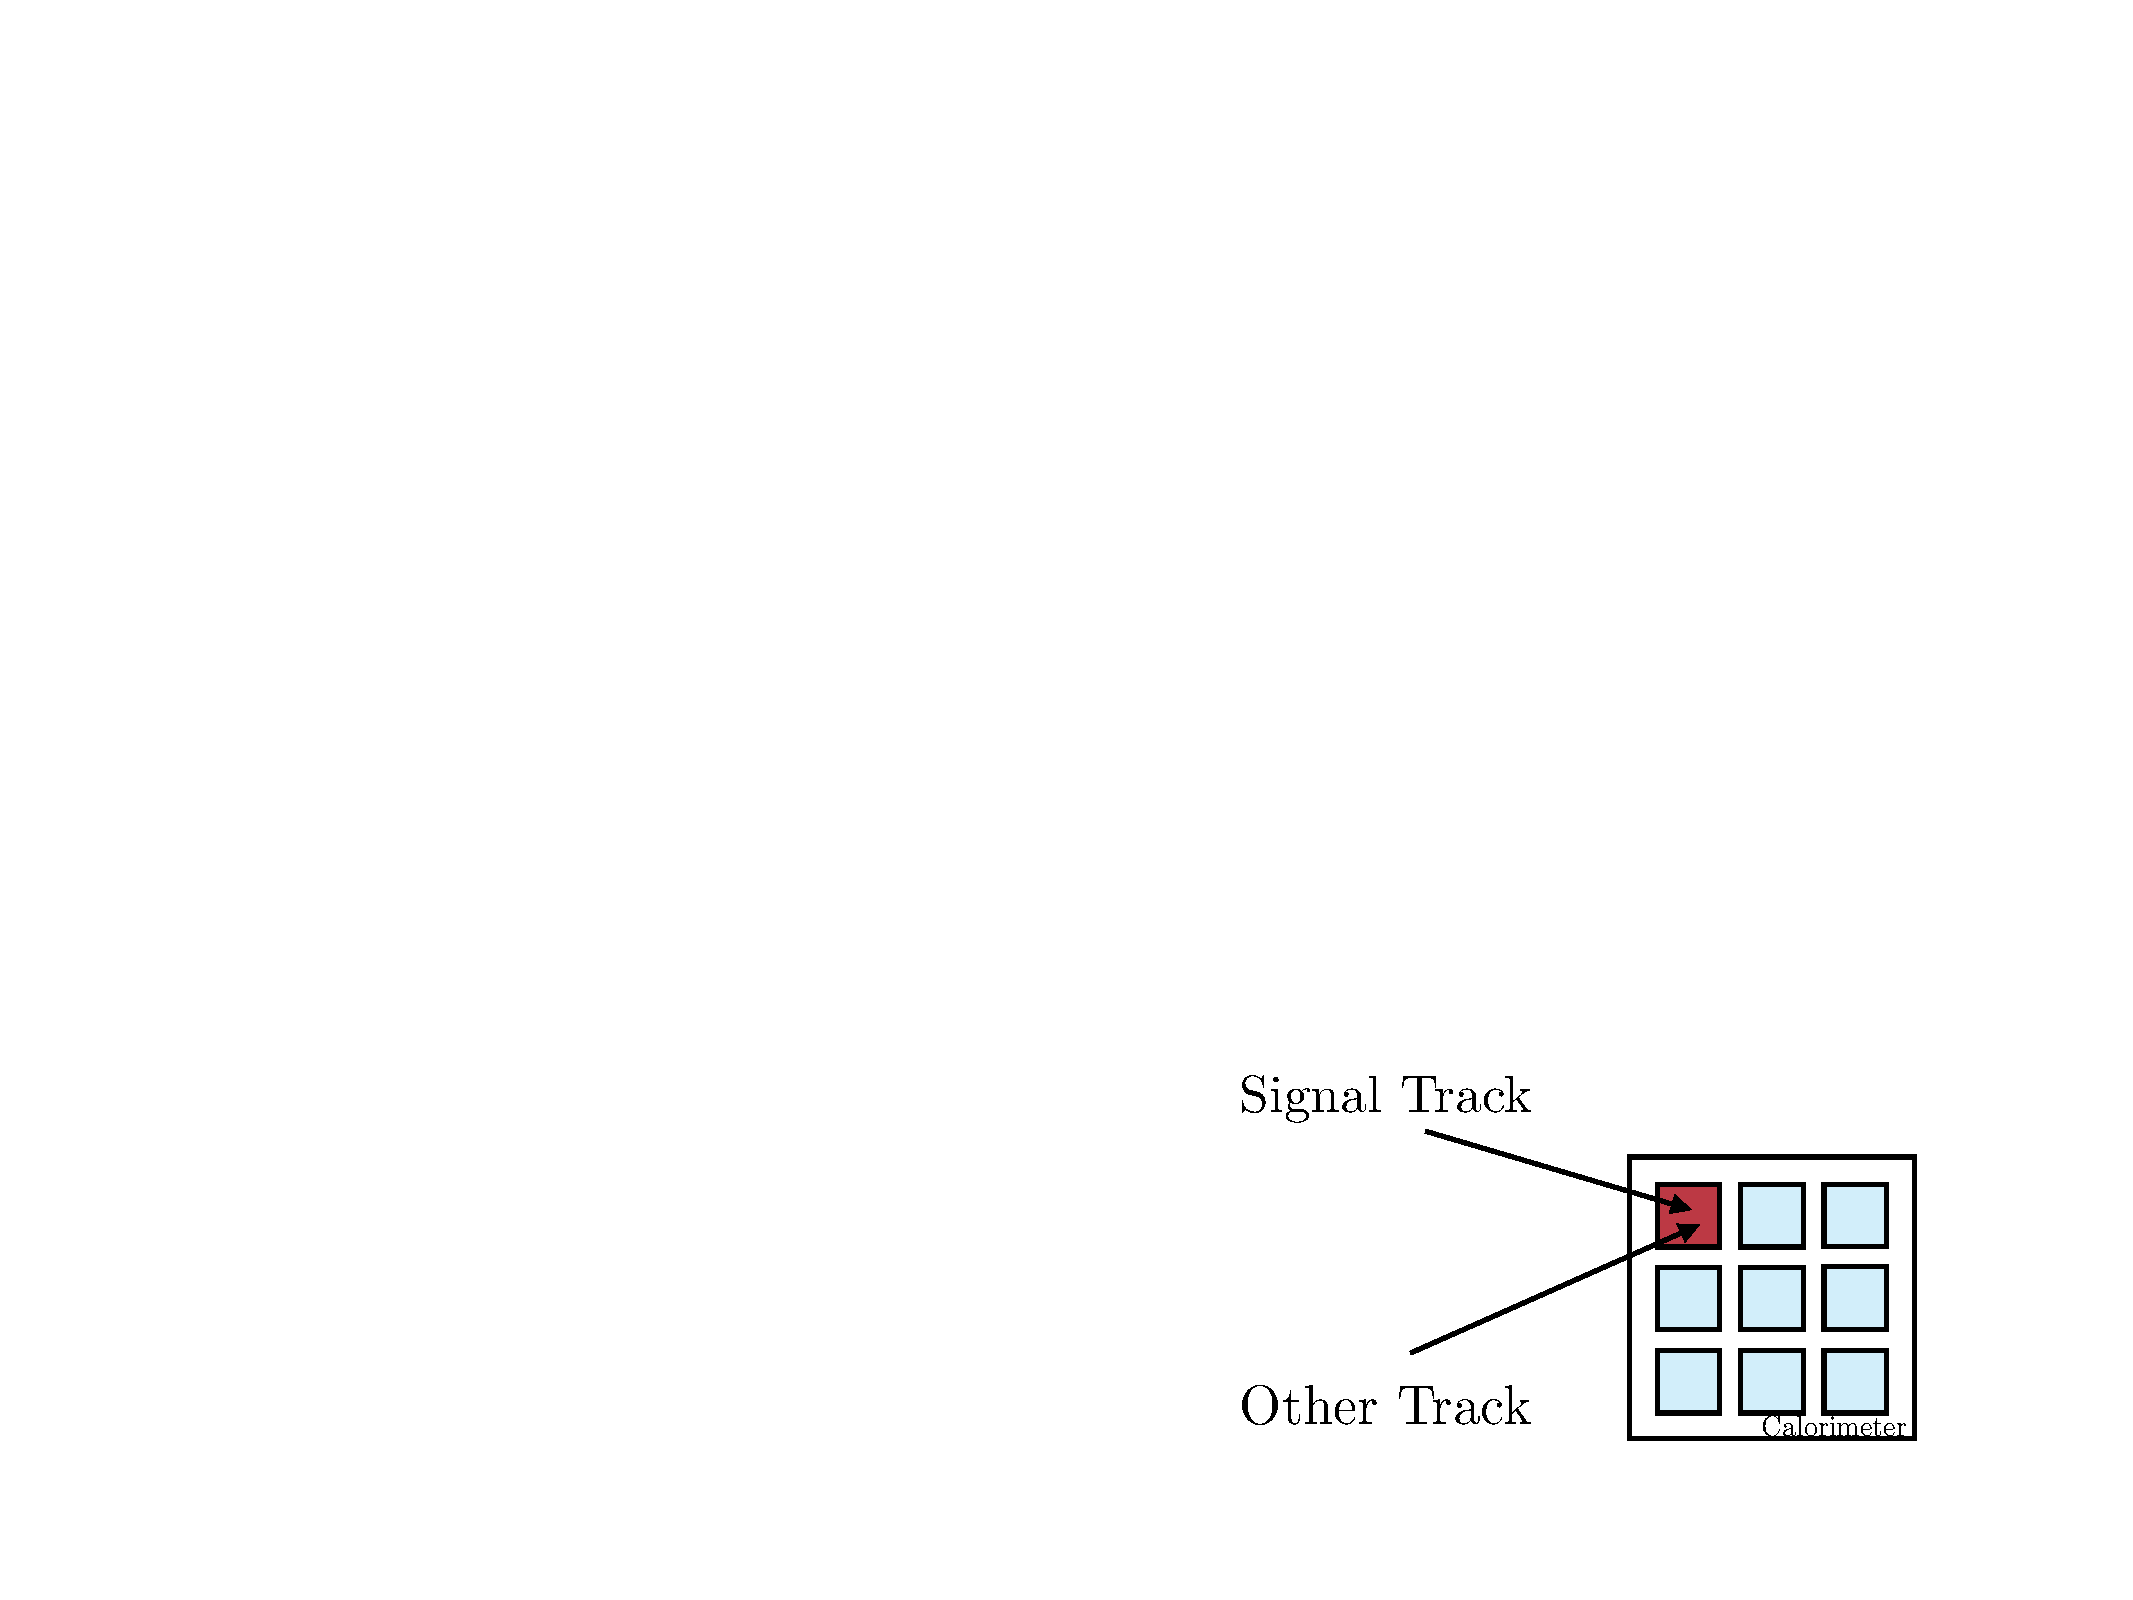
\includegraphics[width=1.0\textwidth]{figs/Selection/Tob.pdf}
        \caption{\texttt{TOB}}
        \label{fig:TOB}
    \end{subfigure}
    \begin{subfigure}[t]{0.4\textwidth}
        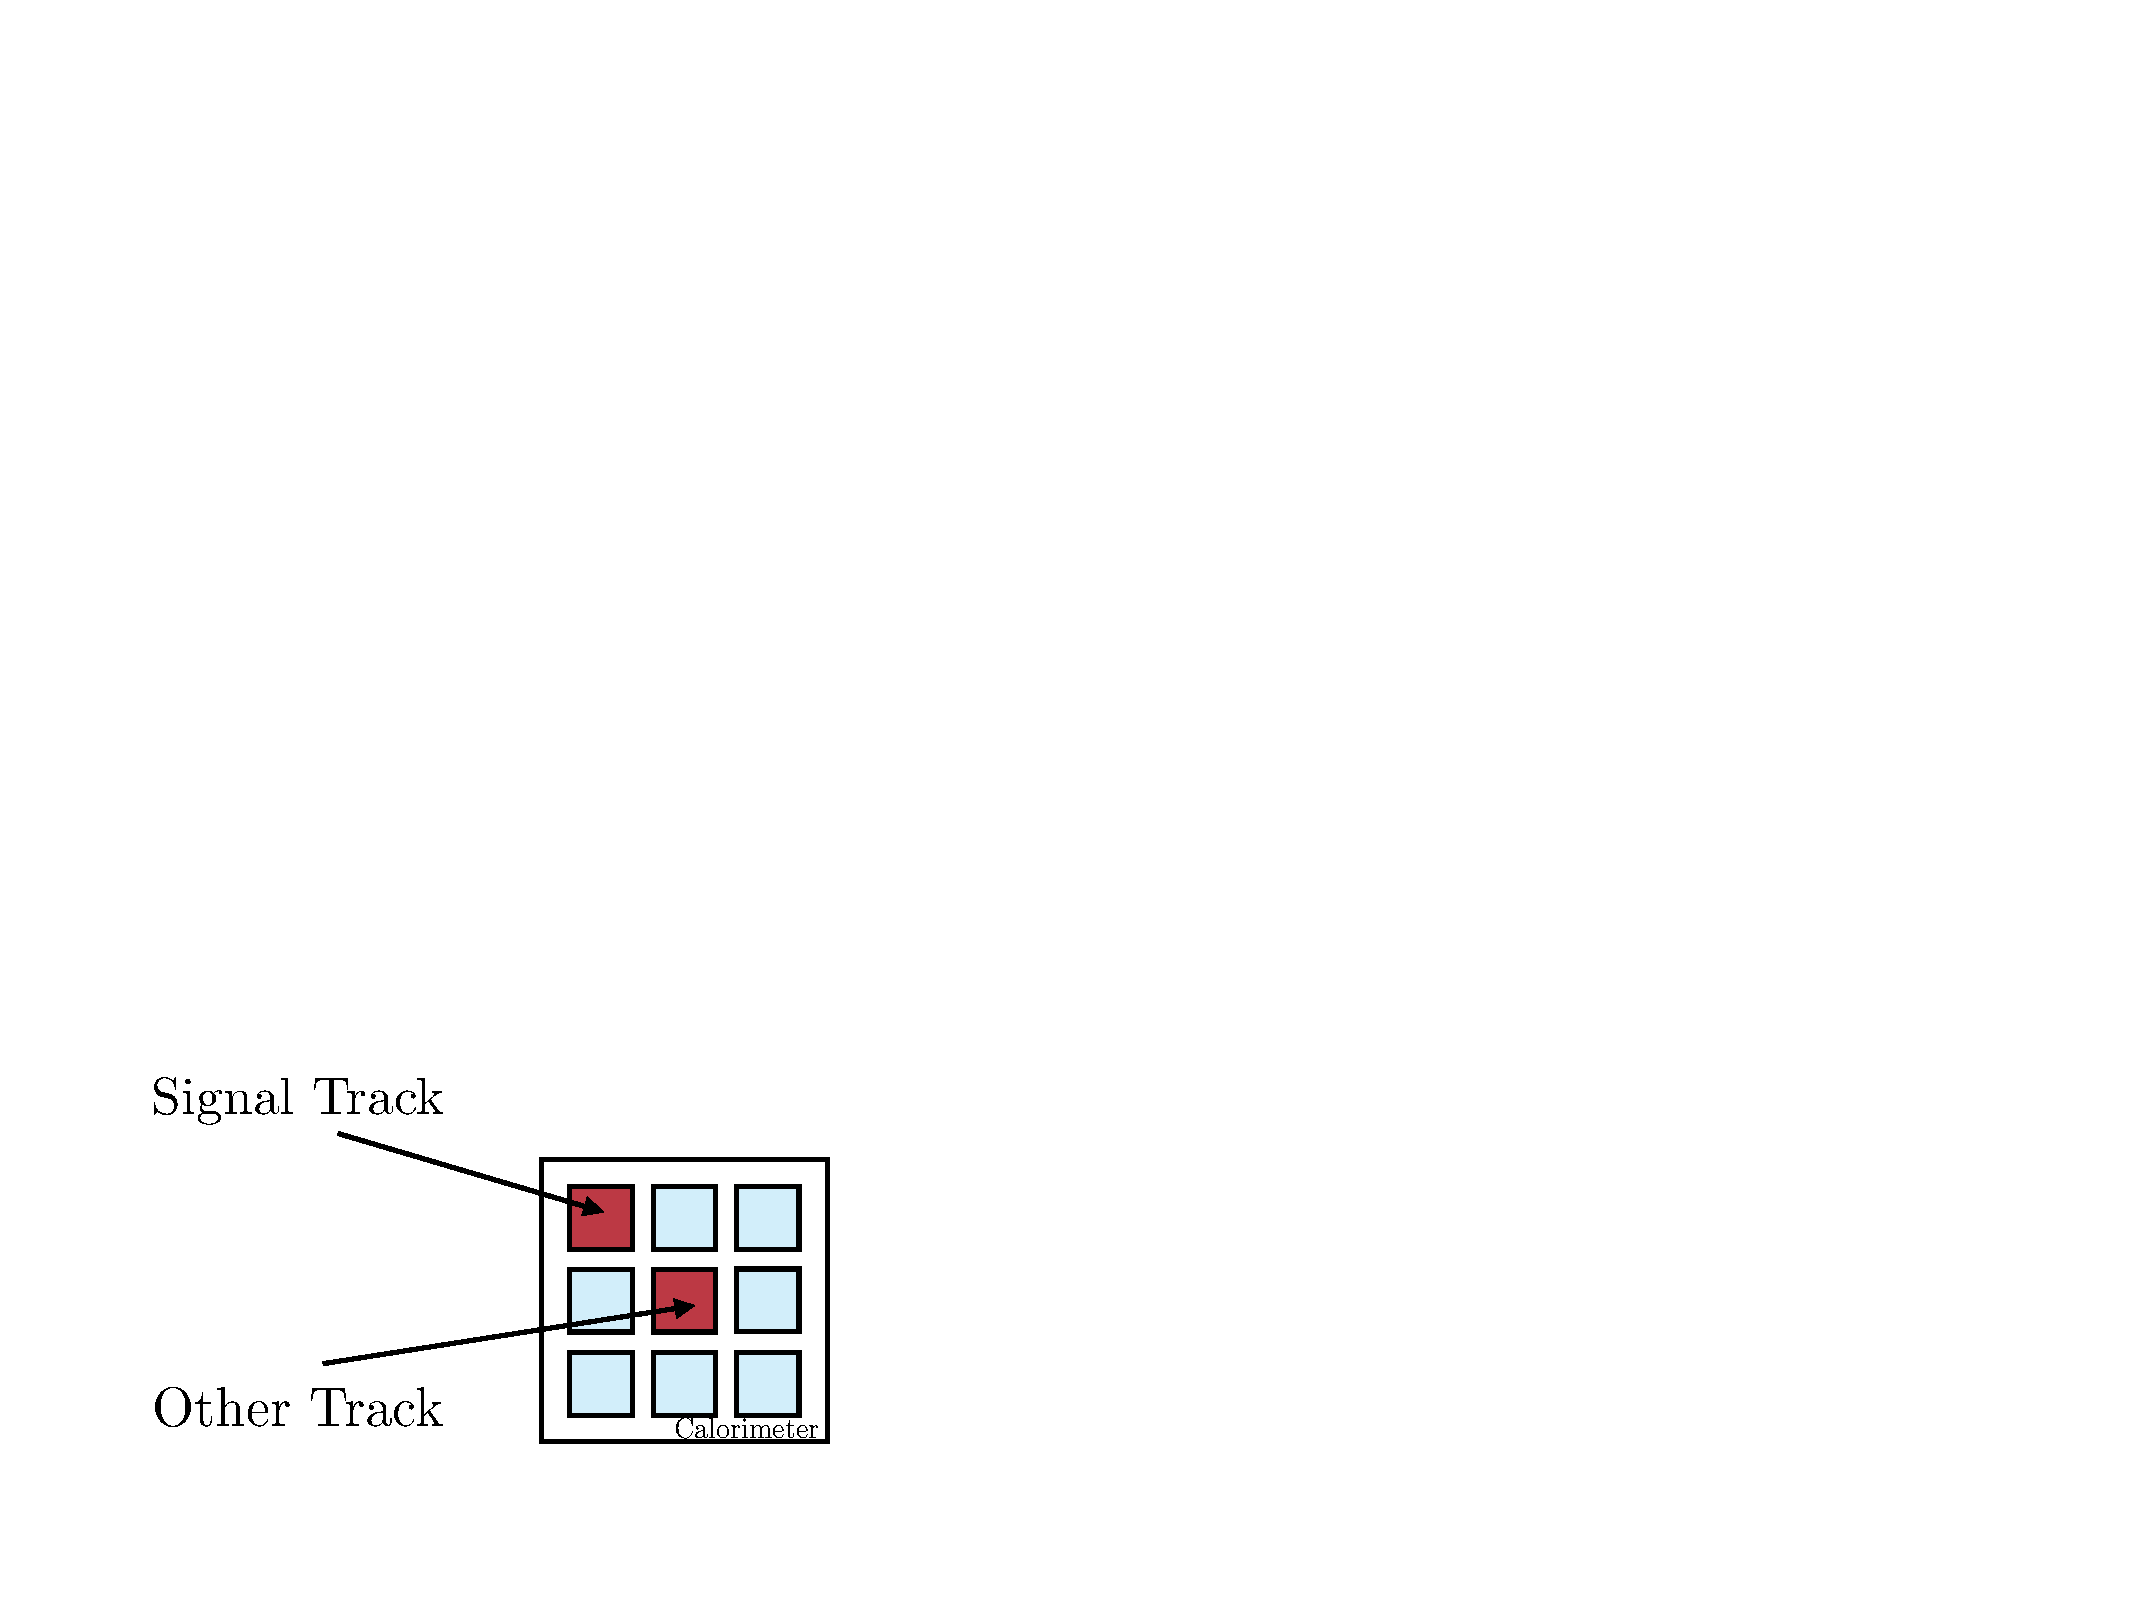
\includegraphics[width=1.0\textwidth]{figs/Selection/TisTos.pdf}
        \caption{\texttt{TOS} and \texttt{TIS}}
        \label{fig:TOSandTIS}
    \end{subfigure}\\
    \caption{Simple schematics of the different trigger matching possibilities, illustrated with one signal track and one non-signal track. Cells with a deposit above the trigger threshold are shown in red. }
    \label{fig:tistostobbing}   
\end{figure}
%%%%%%%%%%%%%%%%%%%%%%%%%%%%%%%%%%%%%%%%%%%%%%%%%%%%%%%%%%


At the hardware trigger stage, the selected candidates are required to be \texttt{TOS} with respect to the hadronic trigger \texttt{L0Hadron}. This ensures the selected candidates were retained due to corresponding deposits in the hadronic calorimeter. 
Alternatively, the logical `or' of each of the hardware sub-systems is combined into a global hardware trigger called \texttt{L0Global}.
Candidates are selected if they are \texttt{TIS} with respect to this combination.
%Alternatively, candidates are selected if they are \texttt{TIS} with respect to the global hardware trigger \texttt{L0Global}; any of the hardware trigger subsystems can contribute to the \texttt{L0Global} decision. 
This allows a second source of decays; those events where the other \bquark quark in a \bquark\bquarkbar pair production has been selected by the trigger. 


This allows candidates that have been retained due another highly energetic decay in the same event to contribute. This could be the decay of hadron resulting from the other \bquark quark in a \bquark\bquarkbar pair production. 

The relative fractions of simulated decays selected by these \texttt{L0Hadron TOS} and \texttt{L0Global TIS} requirements for \decay{\Bp}{\Dsp\phiz} decays decaying to various \Dsp final states are shown in Table~\ref{tab:tis_tos_fractions}. The fractions are normalised to the total number of signal decays passing the \texttt{L0Hadron TOS} or \texttt{L0Global TIS} trigger requirements. 

% \begin{table}[h]
%    \centering
%       \begin{tabular}{lcccc}
%          \hline
%          \Dsp decay mode                &  \texttt{TOS} \& !\texttt{TIS} & \texttt{TIS}\&!\texttt{TOS} &  \texttt{TIS}\&\texttt{TOS}&  \texttt{TIS} or \texttt{TOS}\\
%          \hline 
%          \decay{\Dsp}{\Kp\Km\pip}       & $34.0\%$                   &$40.0\%$                   &$22.9\%$                   &$96.9\%$\\
%          \decay{\Dsp}{\Kp\pim\pip}      & $34.9\%$                   &$38.3\%$                   &$23.8\%$                   &$96.9\%$\\
%          \decay{\Dsp}{\pip\pim\pip}     & $35.9\%$                   &$37.5\%$                   &$23.5\%$                   &$96.9\%$\\
%          \hline
%       \end{tabular}
%    
%    \caption{The fraction of simulated \decay{\Bp}{\Dsp\phiz} decays in each of the hardware trigger categories for the Run I conditions. Here \texttt{TOS} refers to candidates found to be \texttt{TOS} with respect to the \texttt{L0Hadron} trigger, and \texttt{TIS} to candidates found to be \texttt{TIS} with respect to the \texttt{L0Global} requirement. The percentages are given relative to the number of decays passing the reconstruction requirements.}
%    \label{tab:tis_tos_fractions}
% \end{table}
\begin{table}[h]
   \centering
      \begin{tabular}{lccc}
         \hline
         \Dsp decay mode                &  \texttt{TOS} \& !\texttt{TIS} & \texttt{TIS}\&!\texttt{TOS} &  \texttt{TIS}\&\texttt{TOS}\\
         \hline 
         \decay{\Dsp}{\Kp\Km\pip}       & $35.1\%$                   &$41.2\%$                   &$23.7\%$       \\
         \decay{\Dsp}{\Kp\pim\pip}      & $38.0\%$                   &$36.7\%$                   &$25.3\%$       \\
         \decay{\Dsp}{\pip\pim\pip}     & $41.3\%$                   &$31.9\%$                   &$26.8\%$       \\
         \hline
      \end{tabular}
   
   \caption{The fraction of simulated \decay{\Bp}{\Dsp\phiz} decays in each of the hardware trigger categories for the Run I conditions. Here \texttt{TOS} refers to candidates found to be \texttt{TOS} with respect to the \texttt{L0Hadron} trigger, and \texttt{TIS} to candidates found to be \texttt{TIS} with respect to the \texttt{L0Global} requirement. The percentages are given relative to the total number of decay selected by the logical `or' of the two requirements.}
   \label{tab:tis_tos_fractions}
\end{table}

The software trigger stage is split into two parts, \hltone and \hlttwo.
The first stage, \hltone, performs pattern recognition on hits in the \velo and extrapolates tracks forward to the other tracking stations. At least one well reconstructed track is required. This means the track must be significantly displaced from the primary interaction and with $\pt > 1.7 \gevc$. In Run II, this trigger was reimplementing using a multivariate analysis. 

%????????????????????????
% An second algorithm is included to select pairs of high transverse momentum tracks that form a vertex that is displaced from the primary interaction. The signal candidate is required to be \texttt{TOS} with respect to these trigger lines such that two of the $\Dsp h^{+}h^{-}$ candidate tracks passes this requirement.   
%????????????????????????

At the second software stage, \hlttwo, two different algorithms are used to select $\Dsp h^{+}h^{-}$ candidates for this analysis.
The first one uses a multivariate algorithm~\cite{BBDT} to identify the presence of a secondary vertex that has two, three or four tracks and is displaced from any PV. 
%At least one of these charged particles must have a transverse momentum $\pt > 1.7\gevc$ and be inconsistent with originating from a PV. %\chisqip with respect to any primary interaction greater than 16, where \chisqip is defined as the difference in \chisq of a given PV reconstructed with and without the considered track.
This trigger algorithm is referred to as the topological trigger.
The second algorithm selects $\phiz$ candidates decaying to two charged kaons. Each kaon must have a transverse momentum $\pt > 0.8\gevc$ and be inconsistent with originating from a PV. The invariant mass of the kaon pair must be within $20\mevcc$ of the known \phiz mass~\cite{PDG2016}.
This inclusive \phiz line is used to maximise the selection efficiencies as \phiz mesons can contribute directly to \decay{\Bp}{\Dsp\phiz} decays, as well as via the large fractions of \decay{\Dsp}{\phiz\pip} decays that contribute to the \decay{\Dsp}{\Kp\Km\pip} final state.
The relative fractions of simulated \decay{\Bp}{\Dsp\phiz} decays selected by these different trigger algorithms are listed in Table~\ref{tab:topo_incphi_fractions}. The \decay{\Dsp}{\Kp\Km\pip} simulation is generated using an amplitude model that includes the \decay{\Dsp}{\phiz\pip} contribution. As a result, it can be seen that the inclusive \phiz trigger algorithm helps to retain a larger fraction of decays. 

\begin{table}[h]
   \centering
      \begin{tabular}{lccc|c}
         \hline
         \Dsp decay mode                &  \texttt{Topo} \& !\texttt{Phi} & \texttt{Phi}\&!\texttt{Topo} &  \texttt{Topo}\&\texttt{Phi}&  \texttt{Topo} or \texttt{Phi}\\
         \hline 
         \decay{\Dsp}{\Kp\Km\pip}       & $50.9\%$                   &$4.6\%$                   &$43.1\%$                   &$98.7\%$\\
         \decay{\Dsp}{\Kp\pim\pip}      & $67.6\%$                   &$2.7\%$                   &$28.3\%$                   &$98.5\%$\\
         \decay{\Dsp}{\pip\pim\pip}     & $67.5\%$                   &$2.6\%$                   &$28.5\%$                   &$98.7\%$\\
         \hline
      \end{tabular}
   
   \caption{The fraction of simulated \decay{\Bp}{\Dsp\phiz} decays in each of the \hlttwo software trigger categories for the Run I conditions. Here \texttt{Topo} refers to candidates found to be \texttt{TOS} with respect to the topological algorithm, and \texttt{Phi} to candidates found to be \texttt{TOS} with respect to the inclusive \phiz algorithm. The fractions of selected decays are measured relative to the \hltone requirements.}
   \label{tab:topo_incphi_fractions}
\end{table}



\section{Offline selection}

Events passing any trigger requirement are saved to disk for processing offline. The stages of the offline reconstruction are detailed in this section.

\subsection{Selection requirements}
\label{sec:selectionrequirements}

The offline data samples selected by the online trigger system are reconstructed and then further processed in a procedure know within \lhcb as \emph{Stripping}. This centrally managed processing builds candidate topologies from tracks and neutral calorimeter objects in each event according to a set of predefined \emph{Stripping Lines}. Each line builds a specific candidate decay, applying a loose set of preselection requirements, including kinematic, geometric and invariant mass selections. 

The candidate \decay{\Bp}{\Dsp\phiz} and \decay{\Bp}{\Dsp\Kp\Km} decays are built using almost identical set of requirements due to the similar topologies of these decays. The \phiz meson has a lifetime of $(1.55\pm0.01)\times10^{-22}\sec$~\cite{PDG2016}, therefore the kaon decay products effectively originate at the \Bp decay vertex in a similar way to \decay{\Bp}{\Dsp\Kp\Km} decays.  The normalisation channel, \decay{\Bp}{\Dsp\Dzb}, is built similarly, however the difference in lifetime between the \Dzb and \phiz mesons necessitates slightly different selection requirements. The \Dzb meson has a lifetime of $(4.101\pm0.015)\times10^{-13}\sec$, allowing the meson to travel away from the \Bp decay vertex. Sketches of the signal and normalisation decay topologies are shown in Fig.~\ref{fig:topo}.

%%%%%%%%%%%%%%%%%%%%%%%%%%%%%%%%%%%%%%%%%%%%%%%%%%%%%%%%%%
\begin{figure}[!h]
    \centering
    \begin{subfigure}[t]{0.4\textwidth}
        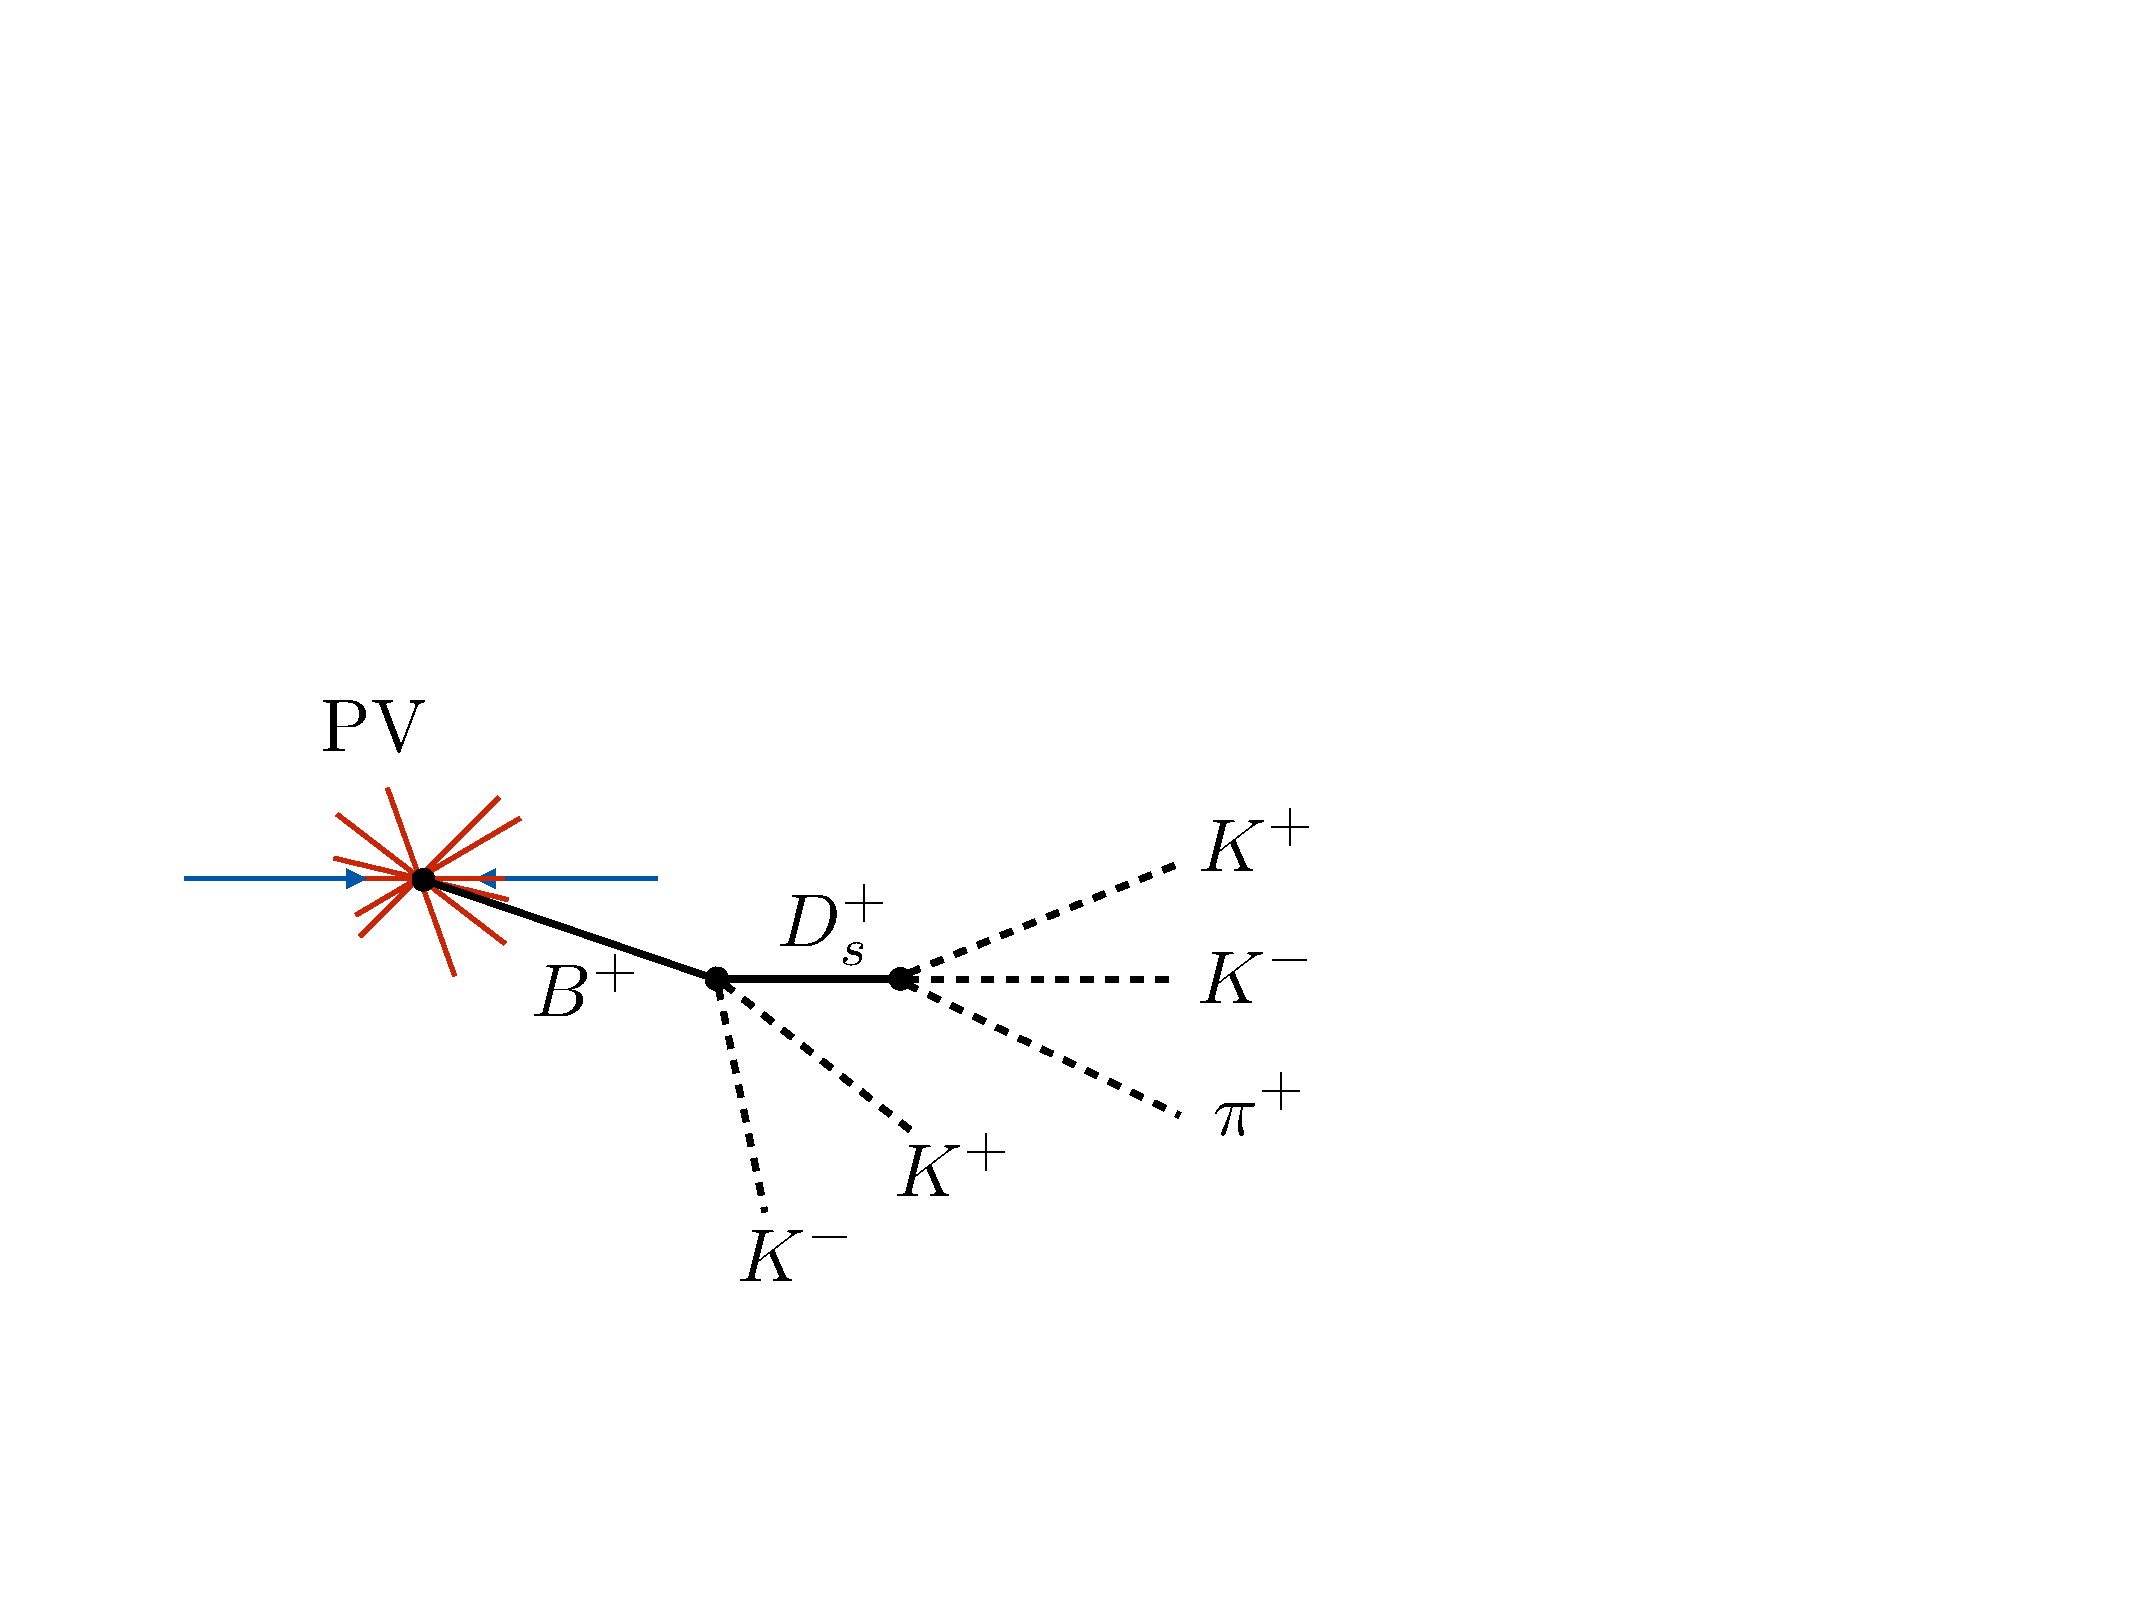
\includegraphics[width=1.0\textwidth]{figs/Selection/B2DsKK_topology.pdf}
        \caption{Signal decays}
    \end{subfigure}%
    \begin{subfigure}[t]{0.4\textwidth}
        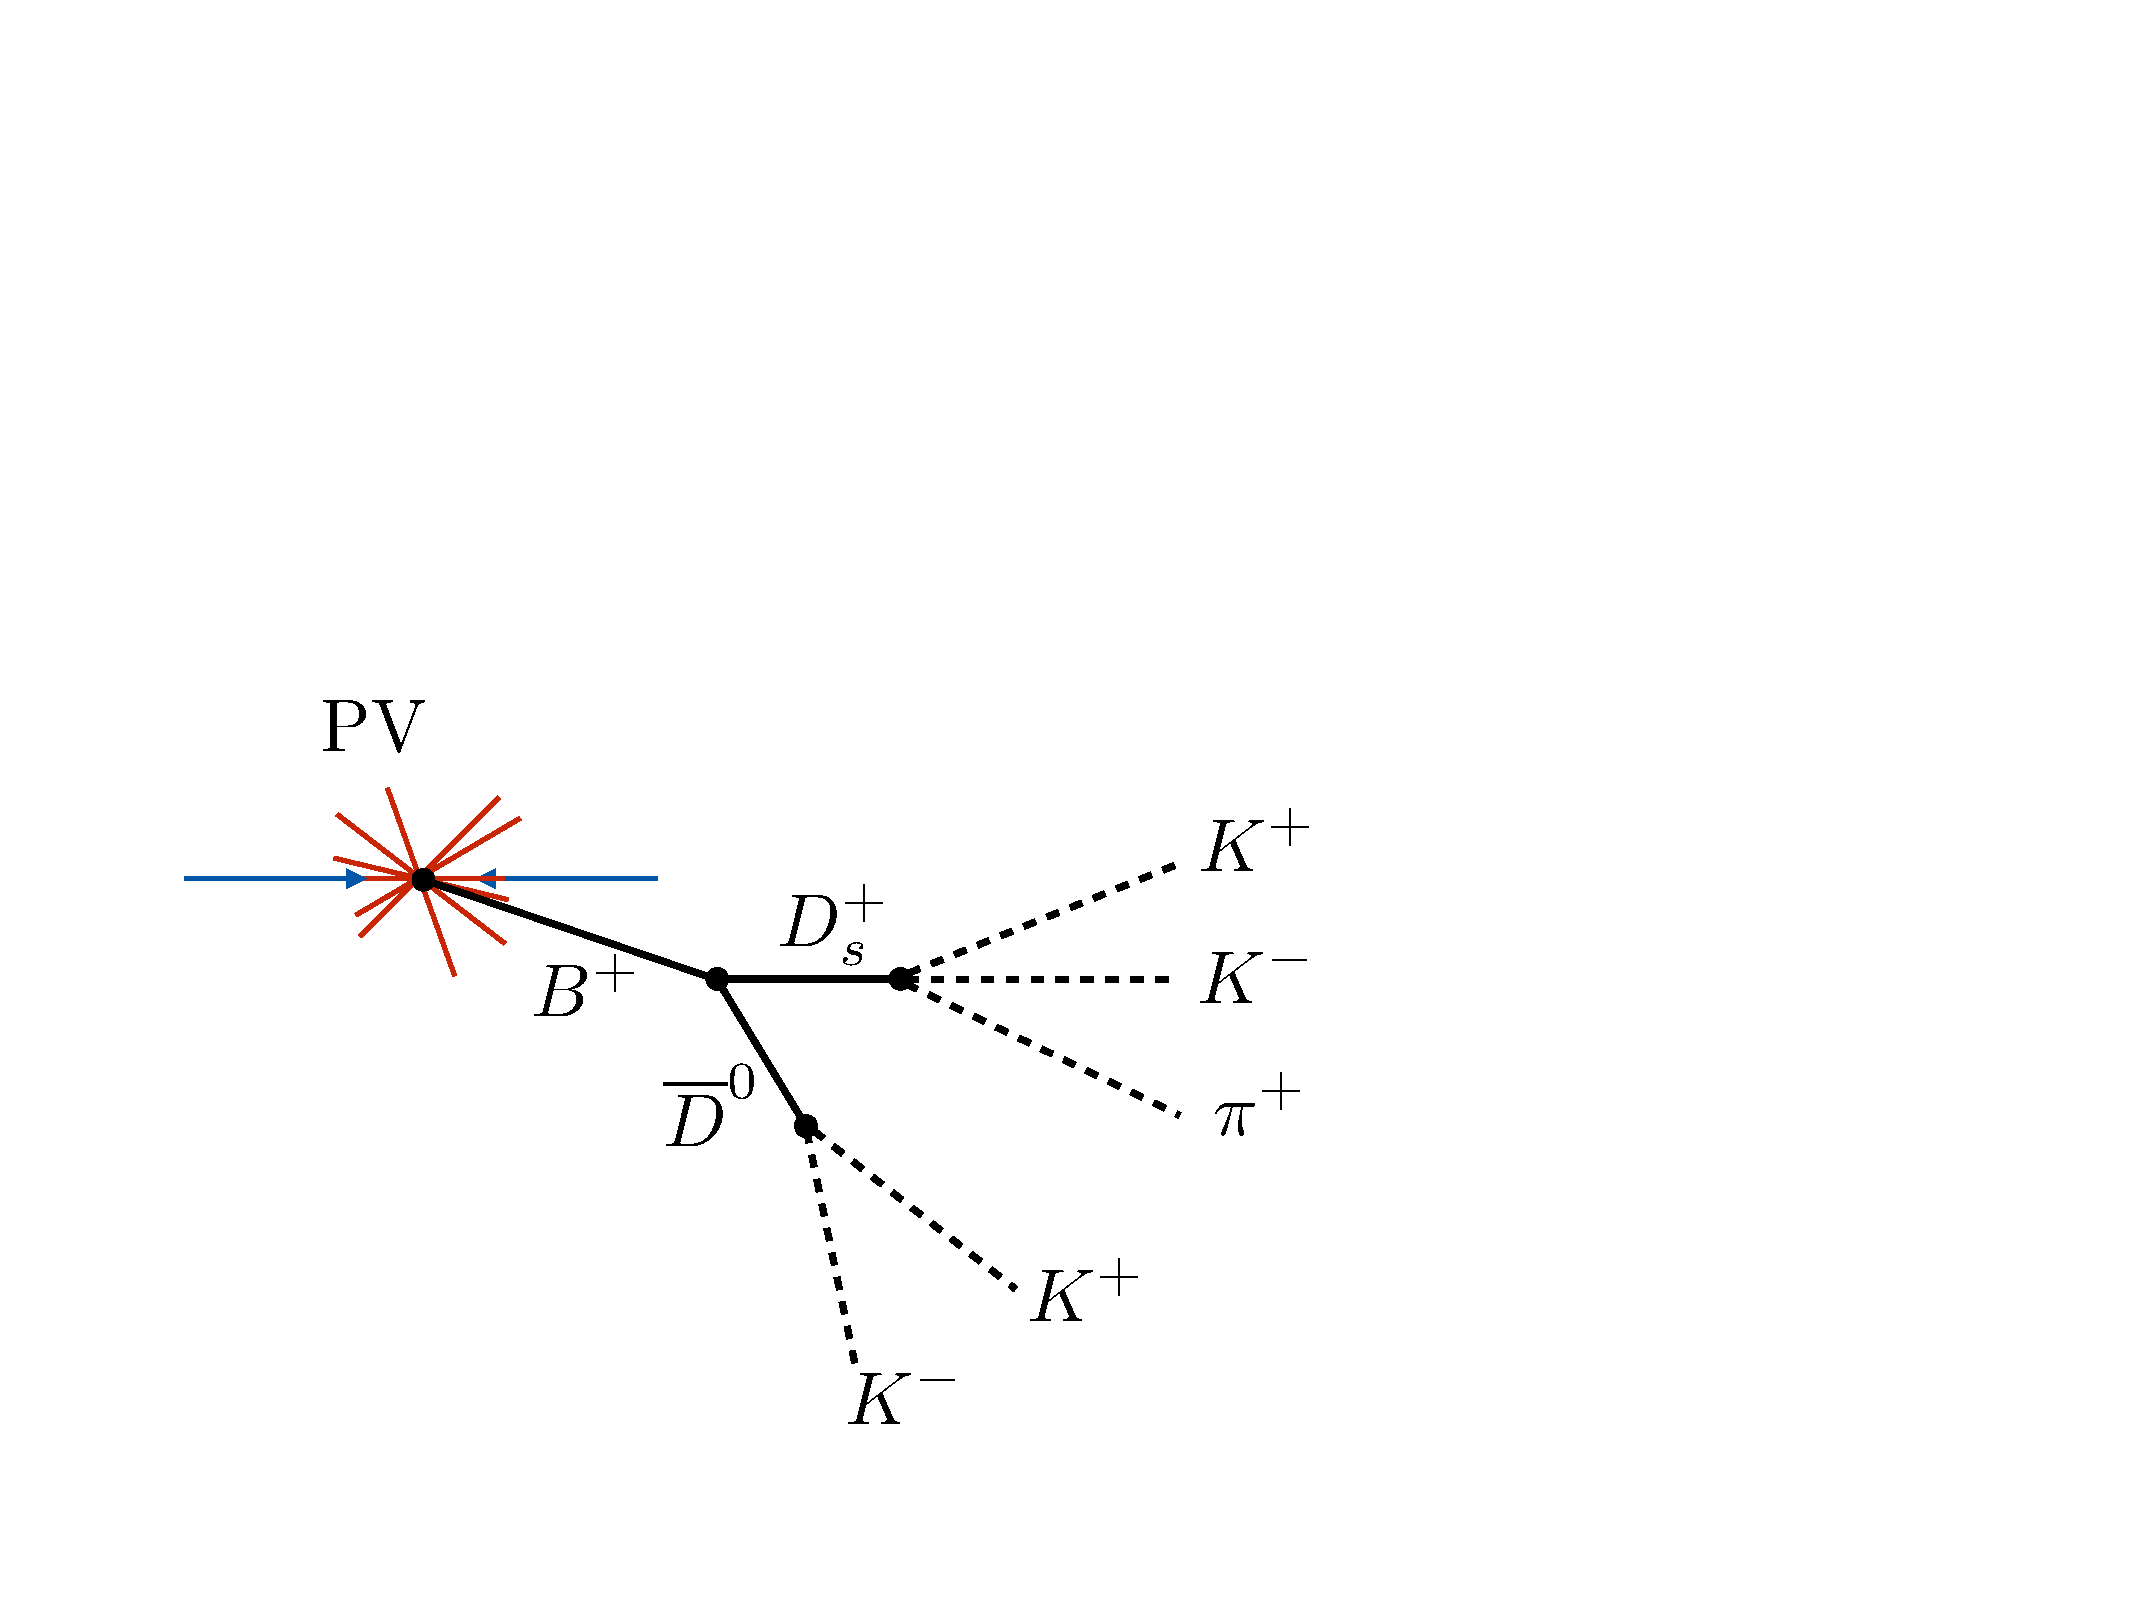
\includegraphics[width=1.0\textwidth]{figs/Selection/B2DsD0_topology.pdf}
        \caption{Normalisation decays}
    \end{subfigure}\\
    \caption{The signal and normalisation decay topologies. The collision of the two protons (blue) results in the primary collision vertex (PV). Many promptly produced tracks (red) originate at the PV. In both cases, the long-lived \Bp meson decay vertex is displaced from the PV. The long-lived charm mesons are also displaced from the \Bp meson decay vertex.}
    \label{fig:topo}   
\end{figure}
%%%%%%%%%%%%%%%%%%%%%%%%%%%%%%%%%%%%%%%%%%%%%%%%%%%%%%%%%%

The candidate \decay{\Bp}{\Dsp\Kp\Km} and \decay{\Bp}{\Dsp\phiz} signal decays and \decay{\Bp}{\Dsp\Dzb} normalisation decay are reconstructed in fully hadronic final states. Both the \Dzb and \phiz mesons are reconstructed using pairs of oppositely charged kaons. The branching fractions are $\BF(\decay{\Dzb}{\Kp\Km})= (3.97 \pm 0.07)\times 10^{-3}$ and $\BF(\decay{\phiz}{\Kp\Km})= (48.9 \pm 0.5)\%$ respectively~\cite{PDG2016}. Although the similar two-body hadronic decay \decay{\Dz}{\Km\pip} has a larger branching fraction than mode chosen for the normalisation channel, $\BF(\decay{\Dz}{\Km\pip})= (3.89 \pm 0.04)\%$, sharing the same final state helps to reduced systematic uncertainties in the ratio of selection efficiencies. Many differences in how pions and kaons interact with the detector can be neglected as they would affect the signal and normalisation channel in the same way.
The \Dsp mesons used in the search for \decay{\Bp}{\Dsp\Kp\Km} decays are reconstructed using the \decay{\Dsp}{\Kp\Km\pip} decay. The search for the rarer \decay{\Bp}{\Dsp\phiz} decay additionally includes the modes \decay{\Dsp}{\pip\pim\pip} and \decay{\Dsp}{\Kp\pim\pip} to increase the sensitivity of the search. The branching fractions for these decays are listed in Table~\ref{tab:dsbranchingfractions}. In each instance the normalisation channel is reconstructed using the same \Dsp decay mode as the signal.  


\begin{table}[h]
   \centering
      \begin{tabular}{lccc}
         \hline
         Decay                            &\Dsp\phiz   &\Dsp\Kp\Km   &  Branching fraction \\
         \hline 
         \decay{\Dsp}{\Kp\Km\pip}         &\checkmark   &\checkmark   & $5.45 \pm 0.17 \%$ \\
         \decay{\Dsp}{\pip\pim\pip}       &\checkmark   & -  & $1.09 \pm 0.05 \%$ \\
         \decay{\Dsp}{\Kp\pim\pip}        &\checkmark   & -   & $0.66 \pm 0.04 \%$ \\
         \hline
      \end{tabular}
   
   \caption{The branching fractions for the different \Dsp decay modes used to reconstruct the signal and normalisation modes. The \Dsp decay modes contributing to the different searches are highlighted.}
   \label{tab:dsbranchingfractions}
\end{table}

%The searches for \decay{\Bp}{\Dsp\phiz} and \decay{\Bp}{\Dsp\Kp\Km} decays employ the use of two different \emph{Stripping Lines} as detailed in Table~\ref{tab:strippinglines}. These differ only in the invariant mass window applied to the $\Kp\Km$ pair used to reconstruct the $\phi$ meson, and in the number of \Dsp decay modes included: the \decay{\Bp}{\Dsp\Kp\Km} line only reconstructs the Cabibbo Favoured (CF) \decay{\Dsp}{\Kp\Km\pip} decay. The \emph{Stripping Line} used to select the normalisation channel \decay{\Bp}{\Dsp\Dzb} is also included in Table~\ref{tab:strippinglines}. This has slightly different requirements allowing the \Dzb meson decay vertex to be be displaced from the \Bp meson decay vertex.


The selection of candidates makes requirements on many different distinguishing characteristics. The definitions of the relevant quantities are as follows:  
\begin{description}
\item \textbf{Mass, $m(X)$:} the invariant mass of the particle, or combination of particles, $X$. 
\item \textbf{Momentum, \ptot:} the magnitude of the total momentum of the particle.
\item \textbf{Transverse momentum, \pt:} The component of the total momentum, \ptot, perpendicular to the proton beam axis (the $z$-axis).
\item \textbf{Decay Time, $\tau$:} the time taken for the candidate to travel from its production vertex to its decay vertex.
\item \textbf{Decay products' \pt scalar sum, $\sum{|\pt|}$:} the sum of the magnitudes of the transverse momentum of the decay products.
\item \textbf{Vertex quality, $\chi^{2}_{\text{VTX}}$:} the minimised value of $\chi^{2}$ per degree of freedom, $\chi^{2}/N_{\text{DOF}}$, as determined in the fit to the vertex location.
\item \textbf{Track quality, $\chi^{2}_{\text{TRK}}$:} the minimised value of $\chi^{2}/N_{\text{DOF}}$ as determined in the fit to the track hits.
\item \textbf{Impact parameter, $\text{IP}$:} The shortest distance between a given extrapolated track direction and a vertex location, as shown in Fig.~\ref{fig:impact_parameter}. 

%%%%%%%%%%%%%%%%%%%%%%%%%%%%%%%%%%%%%%%%%%%%%%%%%%%%%%%%%%
\begin{figure}[!h]
    \centering
    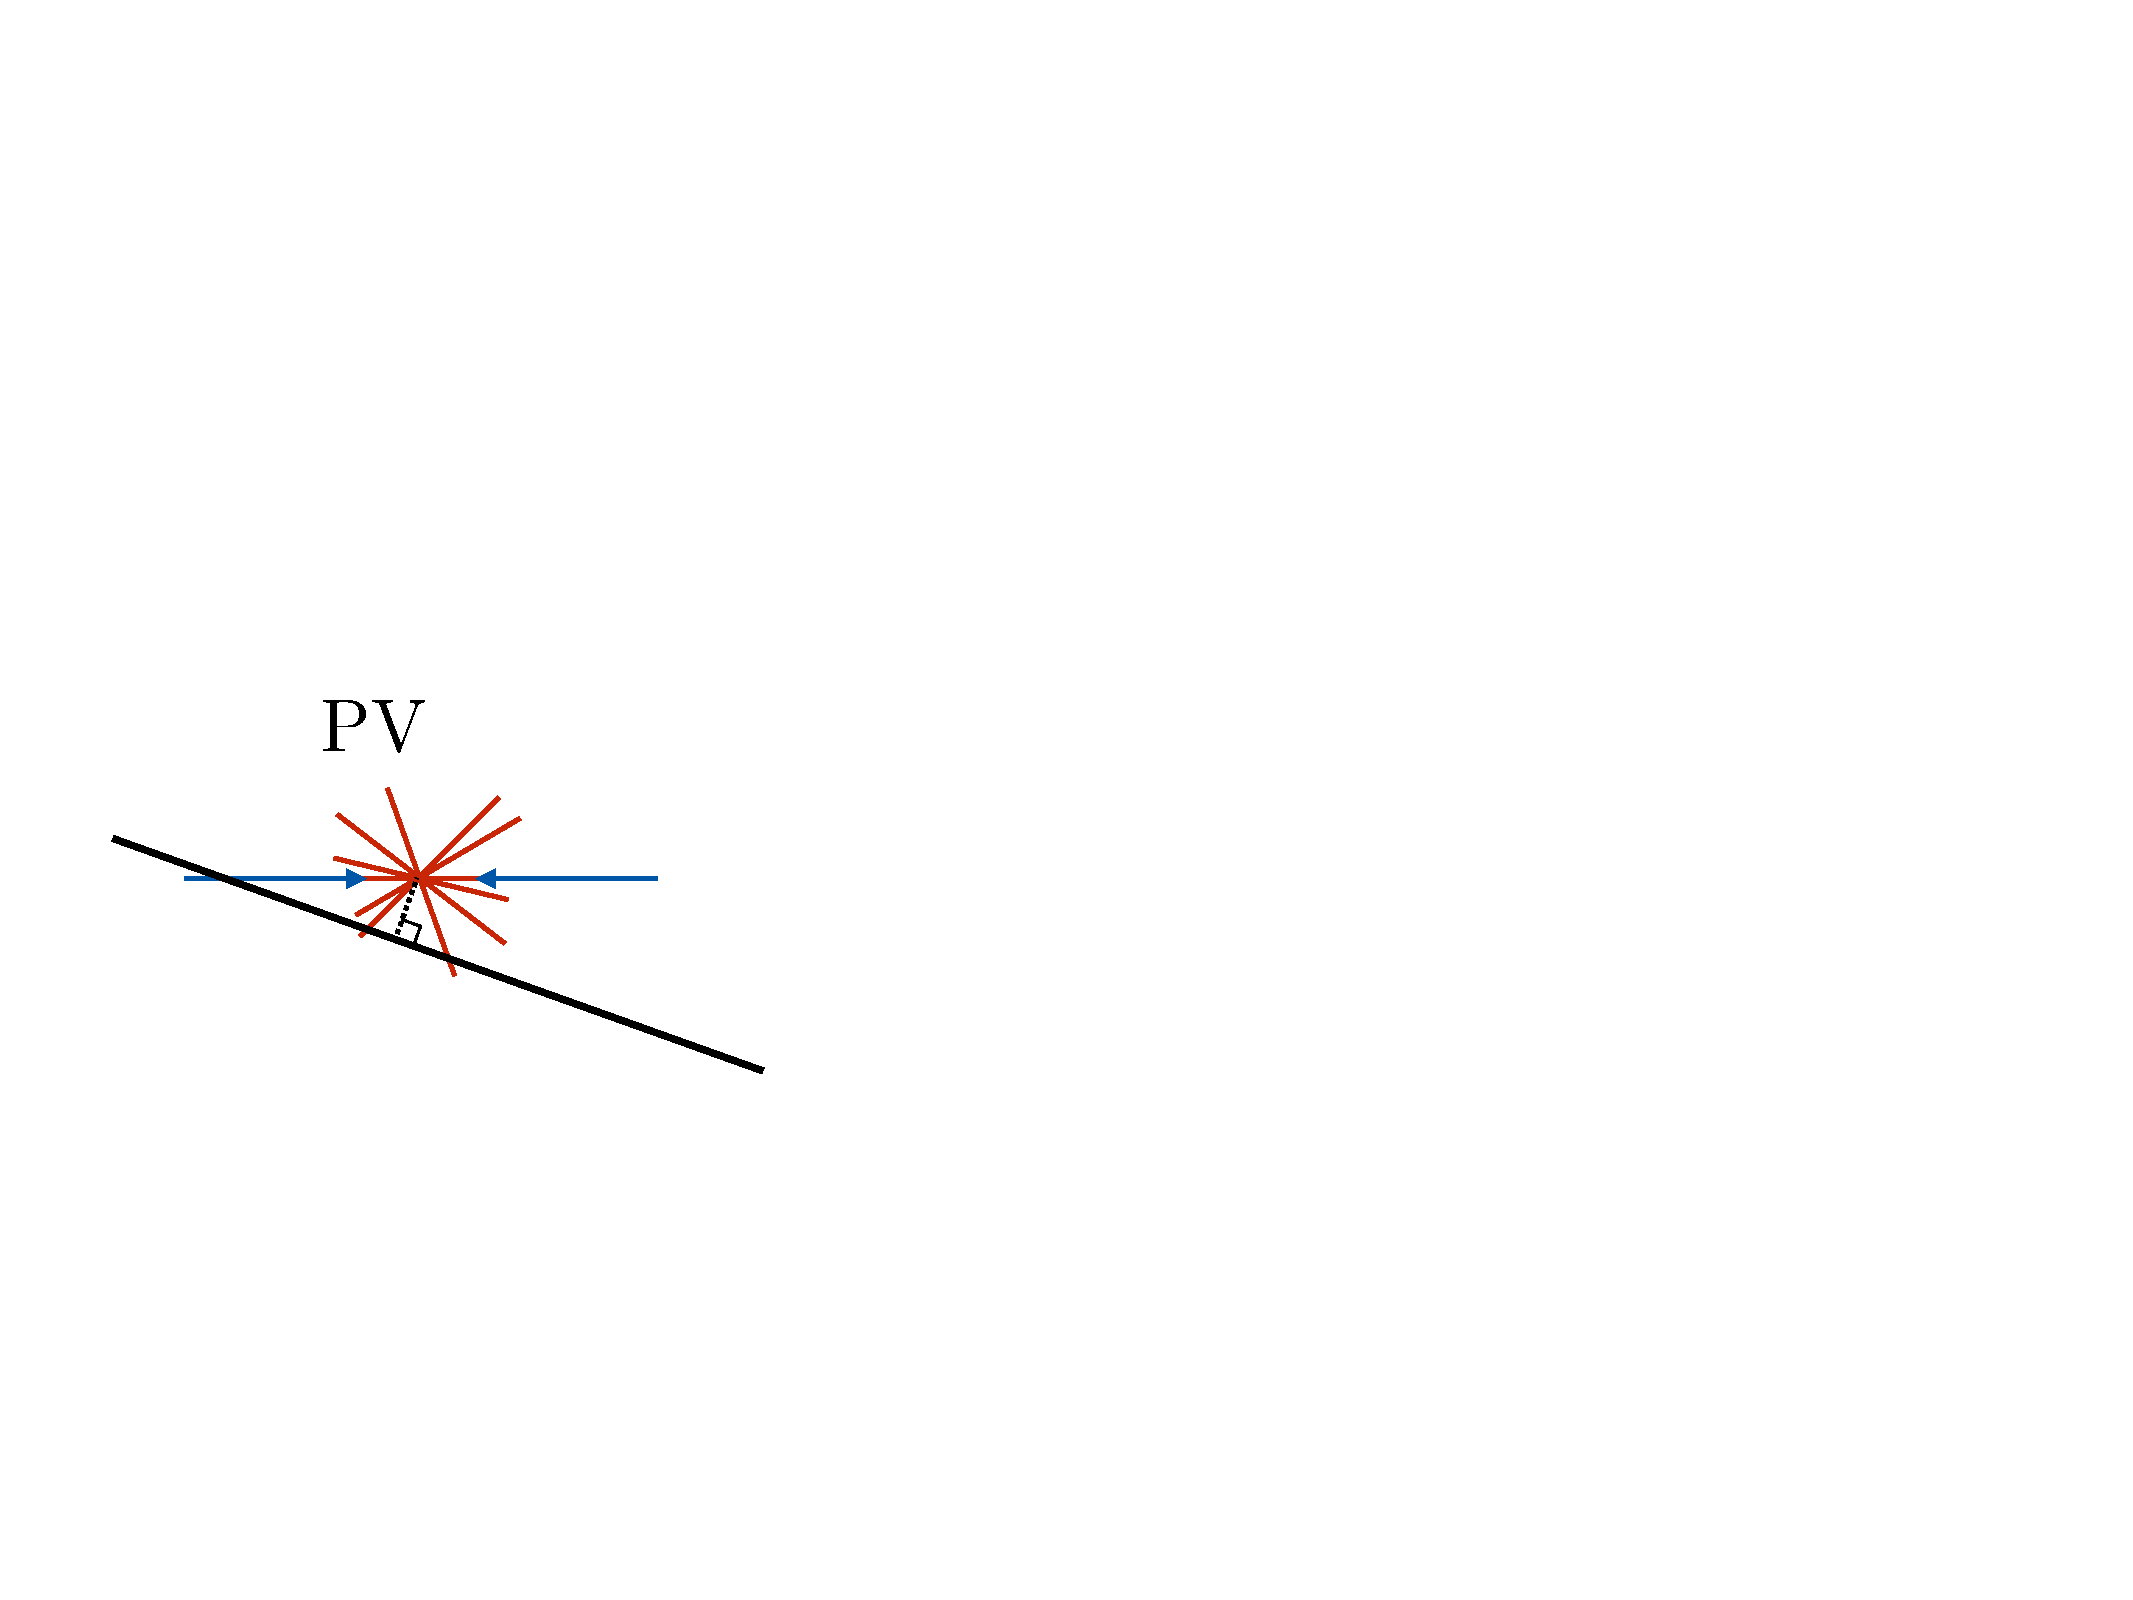
\includegraphics[width=0.4\textwidth]{figs/Selection/Impact_parameter.pdf}
    \caption{Impact parameter (dotted black line) between a track (black) and a vertex.}
    \label{fig:impact_parameter}   
\end{figure}
%%%%%%%%%%%%%%%%%%%%%%%%%%%%%%%%%%%%%%%%%%%%%%%%%%%%%%%%%%

\item \textbf{Impact parameter significance, $\chi^{2}_{\text{IP}}$:} The difference of a given vertex's $\chi^{2}/N_{\text{DOF}}$ with and without a specific track included in the fitting procedure.
\item \textbf{Flight distance significance, $\chi^{2}_{\text{FD}}$:} A measure of how significant the flight distance of a combination of particle is. This is defined as the $\chi^{2}$ associated with the difference in position of the two vertices, $\vec{\mathbf{d}} = \vec{\mathbf{v}}_2 - \vec{\mathbf{v}}_1$, where $\vec{\mathbf{v}}_1$ and $\vec{\mathbf{v}}_1$ are positions of the first and the second vertices. 
\item \textbf{Distance of closest approach, $\text{DOCA}(h,h')$:} The shortest distance between two tracks as shown in Fig~\ref{fig:doca}.
%%%%%%%%%%%%%%%%%%%%%%%%%%%%%%%%%%%%%%%%%%%%%%%%%%%%%%%%%%
\begin{figure}[!h]
    \centering
    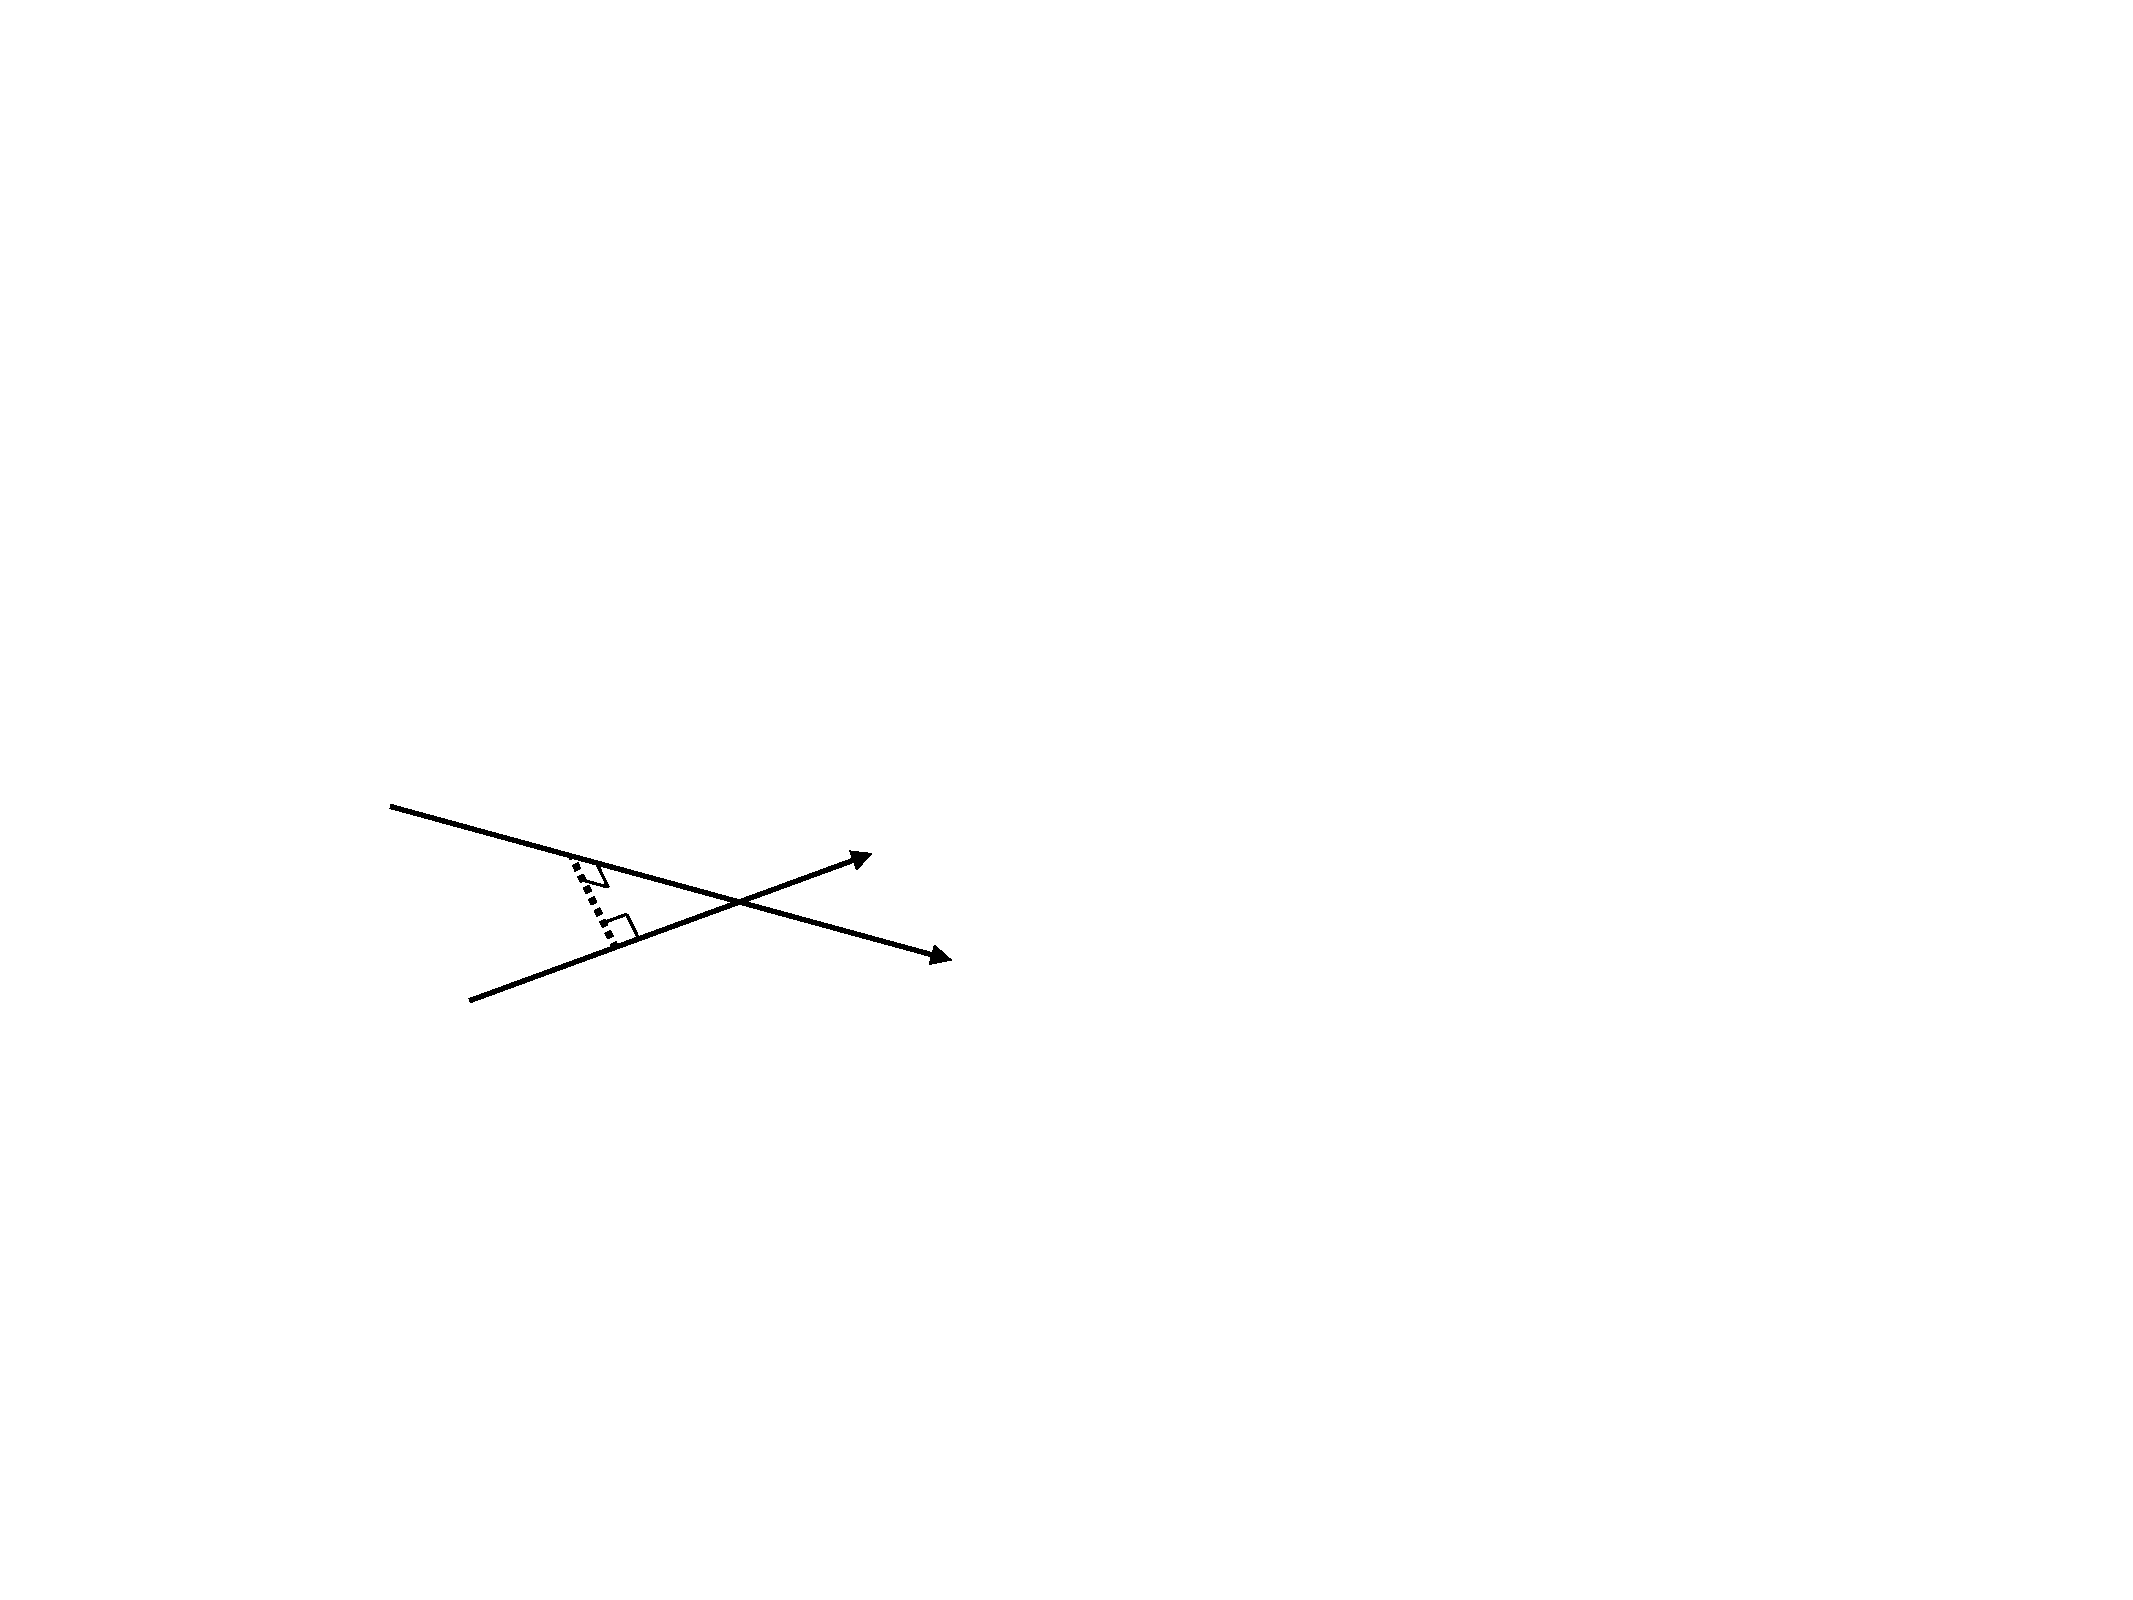
\includegraphics[width=0.4\textwidth]{figs/Selection/DOCA.pdf}
    \caption{Distance of closest approach (dotted black line) between two tracks.}
    \label{fig:doca}   
\end{figure}
%%%%%%%%%%%%%%%%%%%%%%%%%%%%%%%%%%%%%%%%%%%%%%%%%%%%%%%%%%


\item \textbf{Ghost track probability, $P_{\text{Ghost}}$:} This parameter quantifies the probability that a given track is an incorrect combination of tracking stations hits, known as a ghost track. The numerical value is the output of a Neural Network algorithm trained to separate true tracks from ghost tracks using simulated events. Various tracking parameters are inputs to the Neural Network including the number of hits in various tracking stations, the track fit quality and the number of tracks per event. 

\item \textbf{Direction angle:} The angle between a track's momentum vector and the vector connecting the primary vertex and decay vertex as shown in Fig.~\ref{fig:dira}.

%%%%%%%%%%%%%%%%%%%%%%%%%%%%%%%%%%%%%%%%%%%%%%%%%%%%%%%%%%
\begin{figure}[!h]
    \centering
    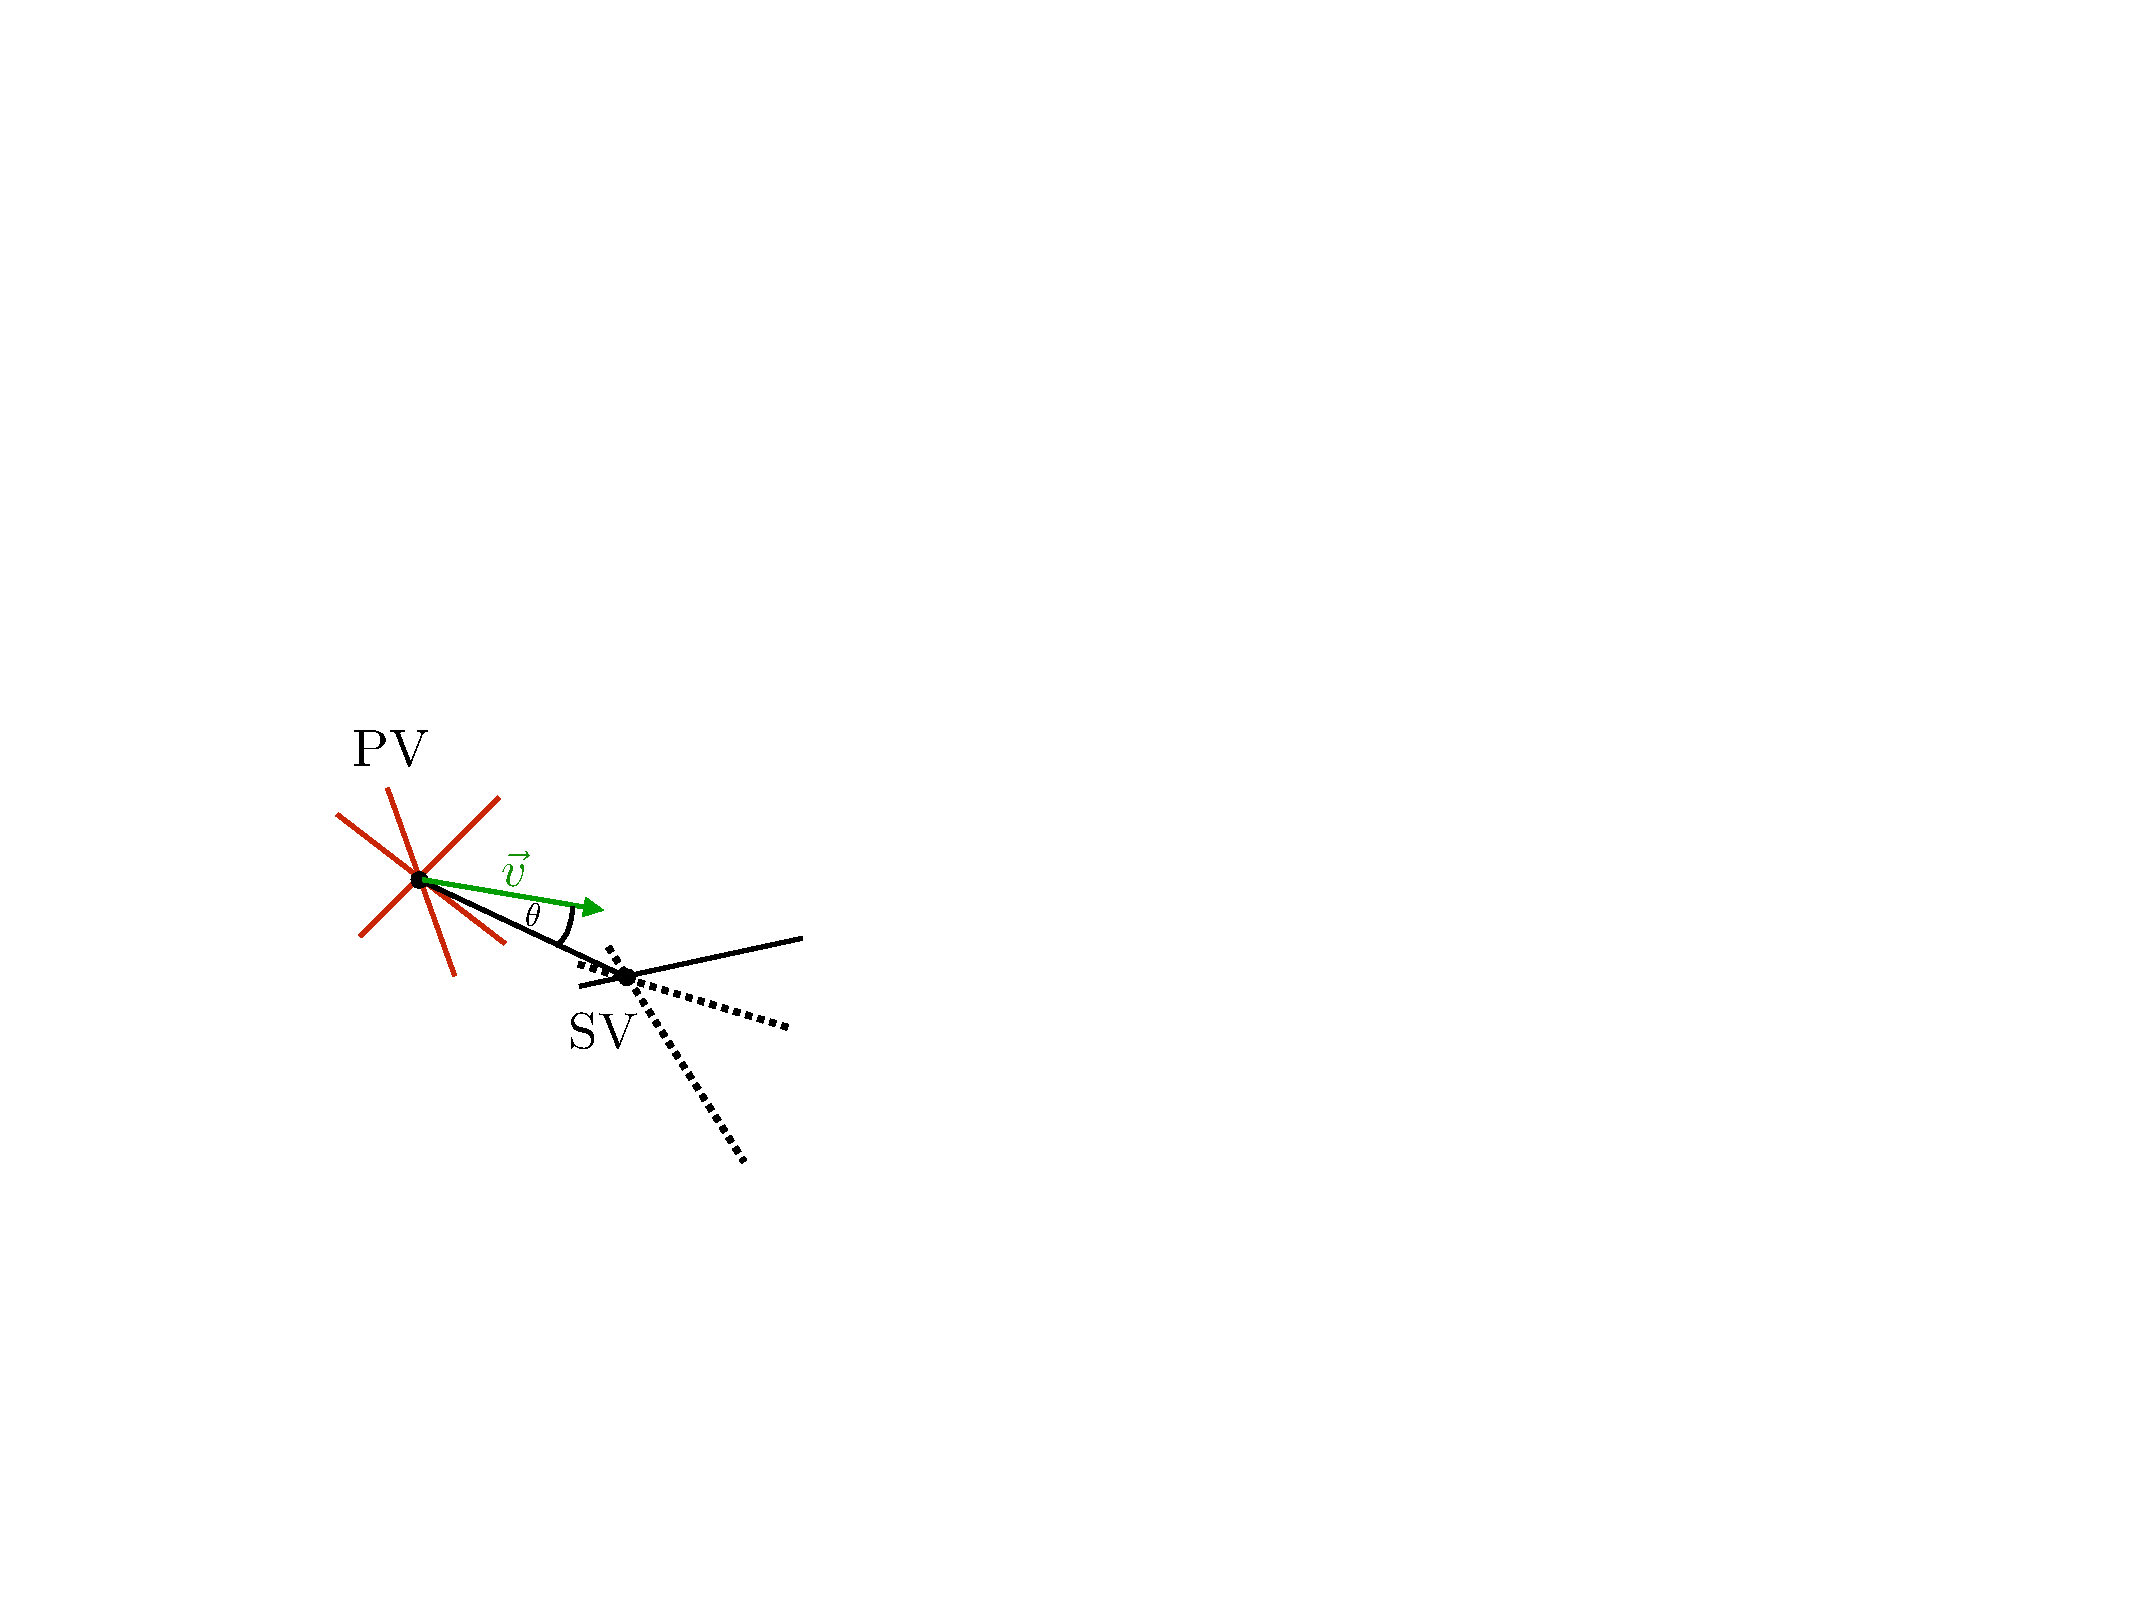
\includegraphics[width=0.4\textwidth]{figs/Selection/DIRA.pdf}
    \caption{Direction angle, $\theta$, between the line joining two vertices, primary vetex (PV) and secondary vertex (SV), and the momentum vector shown in green. The momentum vector corresponds to the momentum of the three tracks contributing to the SV. }
    \label{fig:dira}   
\end{figure}
%%%%%%%%%%%%%%%%%%%%%%%%%%%%%%%%%%%%%%%%%%%%%%%%%%%%%%%%%%


\item \textbf{Particle identification, $\text{PIDK}$:} The different in the log-likelihood of the kaon and pion hypothesis for a given track.  
\end{description}


As the final states are fully hadronic, the candidates are built from the combination of five tracks. Only \emph{long} tracks (those with hits in the \velo and tracking stations) are used to build these mesons. The track $\chi^{2}/N_{\text{DOF}}$ is required to be below $4.0$ to ensure these are well reconstructed. Additionally, they are required to have a total momentum $\ptot > 1000 \mevc$ and the transverse momentum is required to be $\pt > 100 \mevc$.
Due to the long lifetime and high boost of the \Bp and \D mesons, the decay products originate from a vertex that is displaced from the proton-proton collision vertex. In this case the trajectory of the \B or \D decay products do not pass through the primary collision position, as shown in Fig.~\ref{fig:impact_parameter}. A requirement is placed on the significance of the impact parameter between the track and the proton-proton collision vertex of $\chi^{2}_{\text{IP}} > 4$ to ensure all of the tracks used are inconsistent with originating at the primary interaction.  


Loose requirements are placed on \emph{Particle Identification} variables to ensure the tracks are of the required species. These are further tightened as detailed in Section~\ref{sec:pidrequirements}. Incorrect track candidates created by combining unrelated \velo and tracking station hits are suppressed by requiring the ghost track probability, $P_{\text{Ghost}}$, to be less than $0.4$. 

%%%%%% Ds/ D0 and phi construction

The tracks passing these requirements are combined in pairs or triplets to form the \Dsp and \phiz or \Dzb meson candidates.  
For the purpose of forming the \phiz candidates (or \Kp\Km pair), all combinations of two tracks are considered where the tracks are assigned the kaon mass. Only pairs which pass within $0.5\mm$ of one another at their closest point are retained. A number of requirements are imposed to ensure the pair are consistent with coming from a \phiz meson (or \Kp\Km pair) that originated in a \Bp meson decay. The vertex is required to be of good quality, the scalar sum of the transverse momentums must be greater than $1000\mevc$ and the flight distance significance is required to be $\chi^{2}_{\text{FD} } > 16$. Additionally the cosine of the direction angle, defined to be the angle between the momentum vector and flight vector, is required to be $\cos{\theta}>0$, preventing the vertex being backward of the PV when the momentum is in the forward direction. In the search for \decay{\Bp}{\Dsp\phiz} decays, the invariant mass of the two kaons is required to be within $150\mevcc$ of the known \phiz meson mass.  

The \Dzb meson candidates are selecting using a similar parameters, however the exact values of the cuts are changed to reflect the differences in properties of the \phiz and \Dzb mesons. The vertex quality and flight distance significance requirements are tightened to $\chi^{2}/N_{\text{DOF}} < 10$ and $\chi^{2}_{\text{FD} }  > 36$ respectively. Additionally, the scalar \pt sum requirment is increased to $\sum{|\pt|} > 1800 \mevc$ as the decay products tend to have higher transverse momentum. 


The \Dsp mesons candidates are created using combinations of three tracks given the mass hypotheses kaons or pions, depending on the decay mode being constructed. All combinations of three tracks are considered and only those in which all three tracks are within 0.5\mm of one another are retained. As with the \Dzb meson selection, the vertex quality, flight distance significance and scalar \pt sum requirements are $\chi^{2}/N_{\text{DOF}} < 10$, $\chi^{2}_{\text{FD} }  > 36$ and $\sum{|\pt|} > 1800 \mevc$ respectively.

%% B meson construction

The \Bp meson candidates are constructed from all possible combinations of the \Dsp and \phiz or \Dzb meson candidates in each event.
Requirements are placed on these combination to select just those consistent with \Bp mesons.
That is
\begin{itemize}
\item the combination is required to have a lifetime $\tau_{\Bp} > 0.2\ps$, 
\item the direction angle must pass the requirement $\cos{\theta}>0.999$,
\item the impact parameter significance is required to be $\chi^{2}_{\text{IP}} < 25$ to ensure the \Bp meson originated at the primary interaction, 
\item the vertex is required to have a quality of $\chi^{2}/N_{\text{DOF}} < 10$. 
\end{itemize}
%More requirements are additionally placed on the decay products that contribute to the \Bp meson. 
The selection requirements imposed on candidate \decay{\Bp}{\Dsp\phiz} and \decay{\Bp}{\Dsp\Kp\Km} decays in their respective \emph{Stripping Lines} are detailed in Table~\ref{tab:strippinglinecuts}. 


\begin{table}[!h]
\centering
\begin{tabular}{ l l l}
\hline
Particle       & Quantity                       & Requirement                       \\ 
\hline
\Bp            & Mass                           &  $4750 < m(\Dsp\phiz) < 7000\mevcc$    \\  
%               & Transverse Momentum            &  $\pt > 4000 \gevc$               \\  
               & Products \pt scalar sum        &  $\sum{|\pt|} > 5000 \mevc$         \\  
               & Vertex quality                 &  $\chi^{2}/N_{\text{DOF}} < 10$   \\  
               & Lifetime                       &  $\tau_{\Bp} > 0.2\ps$            \\  
               & Impact parameter significance  &  $\chi^{2}_{\text{IP}} < 25$      \\  
               & Direction angle                &  $\cos{\theta}>0.999$             \\  
               & \textit{$>$0 decay products with:}    &                                   \\
               & Momentum                       &  $\ptot > 10000 \mevc$            \\  
               & Transverse momentum            &  $\pt > 1700 \mevc$               \\  
               & Impact parameter significance  &  $\chi^{2}_{\text{IP}} > 16$      \\  
               & Impact parameter               &  $\text{IP} > 0.1\mm$             \\  
               & \textit{$>$1 decay products with:}   &                                   \\
               & Momentum                       &  $\ptot > 5000 \mevc$             \\  
               & Transverse momentum            &  $\pt > 500 \mevc$                \\
%               &                                &                                   \\
\hline  
\Dsp           & Mass                           &  $1770 < m(h^{+}h^{-}h^{+}) < 2068\mevcc$            \\  
               & Products \pt scalar sum        &  $\sum{|\pt|} > 1800 \mevc$         \\ 
               & Distance of closest approach   &  $\text{DOCA}(h^{+},h^{-}) < 0.5\mm$     \\
               & Distance of closest approach   &  $\text{DOCA}(h^{-},h'^{+}) < 0.5\mm$     \\    
               & Distance of closest approach   &  $\text{DOCA}(h^{+},h'^{+}) < 0.5\mm$     \\  
               & Direction angle                &  $\cos{\theta}>0$                 \\  
               & Vertex quality                 &  $\chi^{2}/N_{\text{DOF}} < 10$   \\   
               & Flight distance significance   &  $\chi^{2}_{\text{FD} }  > 36$    \\   
%               &                                &                                   \\  
% \hline
% \phiz          & Mass (only for \decay{\Bp}{\Dsp\phiz})&  $|m(\Kp\Km)-m_{\phiz}| < 150\mevcc$\\ 
%                & Products \pt scalar sum        &  $\sum{|\pt|} > 1000 \mevc$         \\  
%                & Distance of closest approach   &  $\text{DOCA}(\Kp,\Km) < 0.5\mm$  \\  
%                & Direction angle                &  $\cos{\theta}>0$                 \\  
%                & Vertex quality                 &  $\chi^{2}/N_{\text{DOF}} < 16$   \\   
%                & Flight distance significance   &  $\chi^{2}_{\text{FD} }  > 16$    \\   
%               &                                &                                   \\  
\hline
\phiz(\Dzb)    & Mass                           &  $870(1770) < m(X) < 1170(2068)\mevcc$\\ 
               & Products \pt scalar sum        &  $\sum{|\pt|} > 1000~(1800) \mevc$         \\  
               & Distance of closest approach   &  $\text{DOCA}(\Kp,\Km) < 0.5\mm$  \\  
               & Direction angle                &  $\cos{\theta}>0$                 \\  
               & Vertex quality                 &  $\chi^{2}/N_{\text{DOF}} < 16~(10)$   \\   
               & Flight distance significance   &  $\chi^{2}_{\text{FD} }  > 16~(36)$    \\   
%               &                                &                                   \\  
% \hline
% \Dzb           & Mass                           &  $1765 < m(h^{+}h^{-}h^{+}) < 1965\mevcc$\\  
%                & Products \pt scalar sum        &  $\sum{|\pt|} > 1800 \mevc$         \\  
%                & Distance of closest approach   &  $\text{DOCA}(\Kp,\Km) < 0.5\mm$  \\  
%                & Direction angle                &  $\cos{\theta}>0$                 \\  
%                & Vertex quality                 &  $\chi^{2}/N_{\text{DOF}} < 10$   \\   
%                & Flight distance significance   &  $\chi^{2}_{\text{FD} }  > 36$    \\
\hline
\Kpm(\pipm)    & Track quality                  &  $\chi^{2}/N_{\text{DOF}}<4.0$    \\  
               & Transverse momentum            &  $\pt > 100 \mevc$                \\  
               & Momentum                       &  $\ptot > 1000 \mevc$             \\  
               & Impact parameter significance  &  $\chi^{2}_{\text{IP}} > 4$       \\  
               & Ghost track probability        &  $P_{\text{Ghost}} < 0.4$         \\
               & Particle identification        &  $\text{PIDK}>-10$ ($\text{PIDK}<20$)\\  
\hline
\end{tabular}
\caption{Selection requirements for \decay{\Bp}{\Dsp\phiz}, \decay{\Bp}{\Dsp\Kp\Km} and \decay{\Bp}{\Dsp\Dzb} candidates. The \phiz meson invariant mass window is not applied to \decay{\Bp}{\Dsp\Kp\Km} candidates.}
\label{tab:strippinglinecuts}
\end{table}

%%%%%%%%%%%%%%%%%%%%%% DONE %%%%%%%%%%%%%%%%%%%%%%
%B CombCut
%(
% ASUM(
%       SUMTREE(
%                PT,(
%                      ISBASIC | 
%                      (ID=='gamma')
%                   )
%                ,0.0
%             )
%       )>5000*MeV) & 
% (AM<7000*MeV) & 
% (AM>4750*MeV)

% B MotherCut

% (VFASPF(VCHI2/VDOF)<10) &
%(BPVLTIME()>0.2*ps) & 
%(BPVIPCHI2()<25) & 
%(BPVDIRA>0.999)
% (INTREE(
%          HASTRACK & 
%          (P>10000*MeV) & 
%          (PT>1700*MeV) & 
%          (TRCHI2DOF<4.) & 
%          (MIPCHI2DV(PRIMARY)>16) & 
%          (MIPDV(PRIMARY)>0.1*mm) )) & 
% (NINTREE(
%          (
%             ISBASIC & 
%             HASTRACK & 
%             (TRCHI2DOF<4.) & 
%             (PT > 500*MeV) & 
%             (P > 5000*MeV)
%          ) > 1
% )


%X2PiPi
%(ASUM(PT)>1000*MeV) & 
% (AM < 5.2*GeV) & 
% (AHASCHILD(
%             (
%                ISBASIC & 
%                HASTRACK & 
%                (TRCHI2DOF<4.) & 
%                (PT > 500*MeV) & 
%                (P > 5000*MeV)
%             )
%          )
% ) & 
% (ADOCA(1,2)<0.5*mm)

%ADMASS('phi(1020)') < 150*MeV

%PiInput
%(TRCHI2DOF<4.0) & 
% (PT>100*MeV) & 
% (P>1000*MeV) & 
% (MIPCHI2DV(PRIMARY)>4.0) & 
% (TRGHP<0.4)


%D2HHHFilter
%
% (NINGENERATION(
%                ('p+'==ABSID) & 
%                (PIDp < -10),1
%                ) == 0
% ) & 
% (NINGENERATION(   
%                ('K+'==ABSID) & 
%                (PIDK < -10)
%                , 1) == 0
% ) & 
% (NINGENERATION(
%                ('pi+'==ABSID) & 
%                (PIDK > 20)
%                , 1) == 0
% )

% D2HHH CombCut
% (ASUM(PT)>1800*MeV) & 
% (in_range(1769.62*MeV,AWM('K+','K+','pi-'),2068.49*MeV)) & 
% (AHASCHILD(
              
%             ISBASIC & 
%             HASTRACK & 
%             (TRCHI2DOF<4.) & 
%             (PT > 500*MeV) & 
%             (P > 5000*MeV)          
%          )
% ) & 
% (ADOCA(1,3)<0.5*mm) & 
% (ADOCA(2,3)<0.5*mm)

% D2HHH MotherCut
% (VFASPF(VCHI2/VDOF)<10) & 
% (BPVVDCHI2>36) & 
% (BPVDIRA>0)

% PhiMotherCut
% (VFASPF(VCHI2/VDOF)<16) & 
% (BPVVDCHI2>16) & 
% (BPVDIRA>0)


%%%%%%%%%%%%%%%%%%%%%%%%%%%%%%%%%%%%%%%%%%%%%%%%%


%HHPionsInput
%(PT>100*MeV) & (P>2000*MeV)


Two slightly different strategies are used for the normalisation channel selection in the search for \decay{\Bp}{\Dsp\phiz} and \decay{\Bp}{\Dsp\Kp\Km} events.
In the former, a dedicated \decay{\Bp}{\Dsp\Dzb} \emph{Stripping Line} is used to reconstruct the normalisation channel decays.
The \emph{Stripping Line} selection for this line is listed in Table~\ref{tab:strippinglinecuts}.

% \begin{table}[h]
%    \centering
%       \begin{tabular}{l l}
%          \hline
%          Mode & Stripping line \\ 
%          \hline
%          \decay{\Bp}{\Dsp\phiz}        & \texttt{StrippingB2DPhiD2HHHPIDBeauty2CharmLine}    \\
%          \decay{\Bp}{\Dsp\Kp\Km}       & \texttt{StrippingB2DKKD2HHHCFPIDBeauty2CharmLine}   \\
%          \decay{\Bp}{\Dsp\Dzb}         & \texttt{StrippingB2D0DBeauty2CharmLine}             \\
%          \hline
%       \end{tabular}
%    
%    \caption{\emph{Stripping Lines} used in this analysis.}
%    \label{tab:strippinglines}
% \end{table}

The \emph{Stripping Line} used in the search for \decay{\Bp}{\Dsp\Kp\Km} decays covers the full $m(\Kp\Km)$ phase-space. This includes the \Dzb mass such that this line reconstructs both the signal and normalisation channels simultaneously. 
Both modes are selected using this line to reduce systematic uncertainty in the ratio of selection efficiencies.

% \begin{table}[h]
% \centering
% \begin{tabular}{ l l l}
% \hline
% Particles      & Quantity                       & Requirement                       \\ 
% \hline
% \Bp            & Mass                           &  $4750 < m(\Dsp\Dzb) < 7000\mevcc$    \\ 
%                & Products \pt scalar sum        &  $\sum{|\pt|} > 5000 \mevc$         \\  
%                & Vertex quality                 &  $\chi^{2}/N_{\text{DOF}} < 10$   \\  
%                & Lifetime                       &  $\tau_{\Bp} > 0.2\ps$            \\  
%                & Impact parameter significance  &  $\chi^{2}_{\text{IP}} < 25$      \\  
%                & Direction angle                &  $\cos{\theta}>0.999$             \\  
%                & \textit{$>$0 decay products with:}    &                                   \\
%                & Momentum                       &  $\ptot > 10000 \mevc$            \\  
%                & Transverse momentum            &  $\pt > 1700 \mevc$               \\  
%                & Impact parameter significance  &  $\chi^{2}_{\text{IP}} > 16$      \\  
%                & Impact parameter               &  $\text{IP} > 0.1\mm$             \\  
%                & \textit{$>$1 decay products with:}   &                                   \\
%                & Momentum                       &  $\ptot > 5000 \mevc$             \\  
%                & Transverse momentum            &  $\pt > 500 \mevc$                \\
% %               &                                &                                   \\  
% \hline
% \Dsp           & Mass                           &  $1770 < m(h^{+}h^{-}h^{+}) < 2068\mevcc$            \\  
%                & Products \pt scalar sum        &  $\sum{|\pt|} > 1800 \mevc$         \\ 
%                & Distance of closest approach   &  $\text{DOCA}(h^{+},h^{-}) < 0.5\mm$     \\
%                & Distance of closest approach   &  $\text{DOCA}(h^{-},h'^{+}) < 0.5\mm$     \\    
%                & Distance of closest approach   &  $\text{DOCA}(h^{+},h'^{+}) < 0.5\mm$     \\   
%                & Direction angle                &  $\cos{\theta}>0$                 \\  
%                & Vertex quality                 &  $\chi^{2}/N_{\text{DOF}} < 10$   \\   
%                & Flight distance significance   &  $\chi^{2}_{\text{FD} }  > 36$    \\   
% %               &                                &                                   \\  
% \hline
% \Dzb           & Mass                           &  $1765 < m(h^{+}h^{-}h^{+}) < 1965\mevcc$\\  
%                & Products \pt scalar sum        &  $\sum{|\pt|} > 1800 \mevc$         \\  
%                & Distance of closest approach   &  $\text{DOCA}(\Kp,\Km) < 0.5\mm$  \\  
%                & Direction angle                &  $\cos{\theta}>0$                 \\  
%                & Vertex quality                 &  $\chi^{2}/N_{\text{DOF}} < 10$   \\   
%                & Flight distance significance   &  $\chi^{2}_{\text{FD} }  > 36$    \\   
% %               &                                &                                   \\  
% \hline
% \Kpm (\pipm)   & Track quality                  &  $\chi^{2}/N_{\text{DOF}}<4.0$    \\  
%                & Transverse momentum            &  $\pt > 100 \mevc$                \\  
%                & Momentum                       &  $\ptot > 1000 \mevc$             \\  
%                & Impact parameter significance  &  $\chi^{2}_{\text{IP}} > 4$       \\  
%                & Ghost track probability        &  $P_{\text{Ghost}} < 0.4$         \\
%                & Particle identification        &  $\text{PIDK}>-10$ ($\text{PIDK}<20$)\\
% \hline
% \end{tabular}
% 
% \caption{Selection requirements for \decay{\Bp}{\Dsp\Dzb} candidates.}

% \label{tab:strippinglinecuts}
% \end{table}



% D2KKPi Mother
% (VFASPF(VCHI2/VDOF)<10) & (BPVVDCHI2>36) & (BPVDIRA>0)



% D2KKPi Comb12 
% (ADOCA(1,2)<0.5*mm)


% D2KKPi Comb
% 
% (ASUM(PT)>1800*MeV) & 
% (in_range(1769.62*MeV,AWM('K-','K-','pi+'),2068.49*MeV)) & 
% (AHASCHILD(
%             ISBASIC & 
%             HASTRACK & 
%             (TRCHI2DOF<4.) & 
%             (PT > 500*MeV) & 
%             (P > 5000*MeV)  
%          )  
% ) & 
% (ADOCA(1,3)<0.5*mm) & 
% (ADOCA(2,3)<0.5*mm)



% K input 
% (TRCHI2DOF<4.0) & (PT>100*MeV) & (P>1000*MeV) & (MIPCHI2DV(PRIMARY)>4.0) & (TRGHP<0.4)


% D2KK Mother
% 
% (VFASPF(VCHI2/VDOF)<10) & 
% (BPVVDCHI2>36) & 
% (BPVDIRA>0)




% D2KK Comb
% 
% (ASUM(PT)>1800*MeV) & 
% (in_range(1764.84*MeV,AWM('K+','K-'),1964.84*MeV)) & 
% (AHASCHILD(
%          ISBASIC & 
%          HASTRACK & 
%          (TRCHI2DOF<4.) & 
%          (PT > 500*MeV) & 
%          (P > 5000*MeV)    
%       )
% ) & 
% (ADOCA(1,2)<0.5*mm)

% D2HH
% (NINGENERATION(('p+'==ABSID) & (PIDp < -10),1) == 0) & (NINGENERATION(('K+'==ABSID) & (PIDK < -10), 1) == 0) & (NINGENERATION(('pi+'==ABSID) & (PIDK > 20), 1) == 0)


% B mother cut
% (VFASPF(VCHI2/VDOF)<10) & 
% (
%    INTREE(HASTRACK & 
%    (P>10000*MeV) & 
%    (PT>1700*MeV) & 
%    (TRCHI2DOF<4.) & 
%    (MIPCHI2DV(PRIMARY)>16) & 
%    (MIPDV(PRIMARY)>0.1*mm))
% ) & 
% (
%    NINTREE( 
%             ISBASIC & 
%             HASTRACK & 
%             (TRCHI2DOF<4.) & 
%             (PT > 500*MeV) & 
%             (P > 5000*MeV)     
%          ) > 1
% ) & 
% (BPVLTIME()>0.2*ps) & 
% (BPVIPCHI2()<25) & 
% (BPVDIRA>0.999)


% B comb
% (ASUM(
%    SUMTREE(PT,ISBASIC,0.0) )>5000*MeV
% ) & 
% (AM<7000*MeV) & 
% (AM>4750*MeV)

%%%%%%%%%%%%% done %%%%%%%%%%%


%\clearpage


\subsection{Particle identification requirements}
\label{sec:pidrequirements}
%Particle identification variables help to determine the species of tracks passing though the \lhcb detector. Using information from the RICH sub-detectors, the likelihood of different mass hypotheses are compared to the pion hypothesis. Loose 
Requirements are made on the kaon hypothesis PID variable to reduce the contribution from other types of hadrons and background from other \bquark-hadron decays with misidentified hadrons. 
The parameter is defined to be
\begin{equation}
\text{PIDK} = \Delta \log(K - \pi) = \log\mathcal{L}(K) - \log\mathcal{L}(\pi)
\end{equation}
where $\mathcal{L}(K)$ and $\mathcal{L}(\pi)$ are the likelihoods of the kaon and pion hypotheses respectively.
The requirements placed on each decay product are listed in Table~\ref{tab:selection_pid_cuts}.

\begin{table}[h]
   \centering
      \begin{tabular}{l l l}
         \hline
         Decay mode & Species & PID requirement\\ 
         \hline
         \decay{\phiz}{\Kp\Km}      & \Kp    & $\text{PIDK} > 0$  \\
                                    & \Km    & $\text{PIDK} > 0$  \\
         \hline
         \decay{\Dzb}{\Kp\Km}       & \Kp    & $\text{PIDK} > 0$  \\
                                    & \Km    & $\text{PIDK} > 0$  \\
         \hline
         \decay{\Dsp}{\Kp\Km\pip}   & \Kp    & $\text{PIDK} > -5$ \\
                                    & \Km    & $\text{PIDK} > -5$ \\
                                    & \pip   & $\text{PIDK} < 5$  \\
         \hline
         \decay{\Dsp}{\pip\pim\pip} & \pip   & $\text{PIDK} < 5$  \\
                                    & \pim   & $\text{PIDK} < 5$  \\
                                    & \pip   & $\text{PIDK} < 5$  \\
         \hline
         \decay{\Dsp}{\Kp\pim\pip}  & \Kp    & $\text{PIDK} > -5$ \\
                                    & \pim   & $\text{PIDK} < 5$  \\
                                    & \pip   & $\text{PIDK} < 5$  \\
         \hline
      \end{tabular}
   \caption{Particle identification requirements applied to kaons and pions.}
   \label{tab:selection_pid_cuts}
\end{table}

The distribution of PIDK for pions and kaons is shown in Fig.~\ref{fig:selection_PIDK_distribution} as determined from data calibration samples.
%%%%%%%%%%%%%%%%%%%%%%%%%%%%%%%%%%%%%%%%%%%%%%%%%%%%%%%%%%
\begin{figure}[!h]
    \centering
        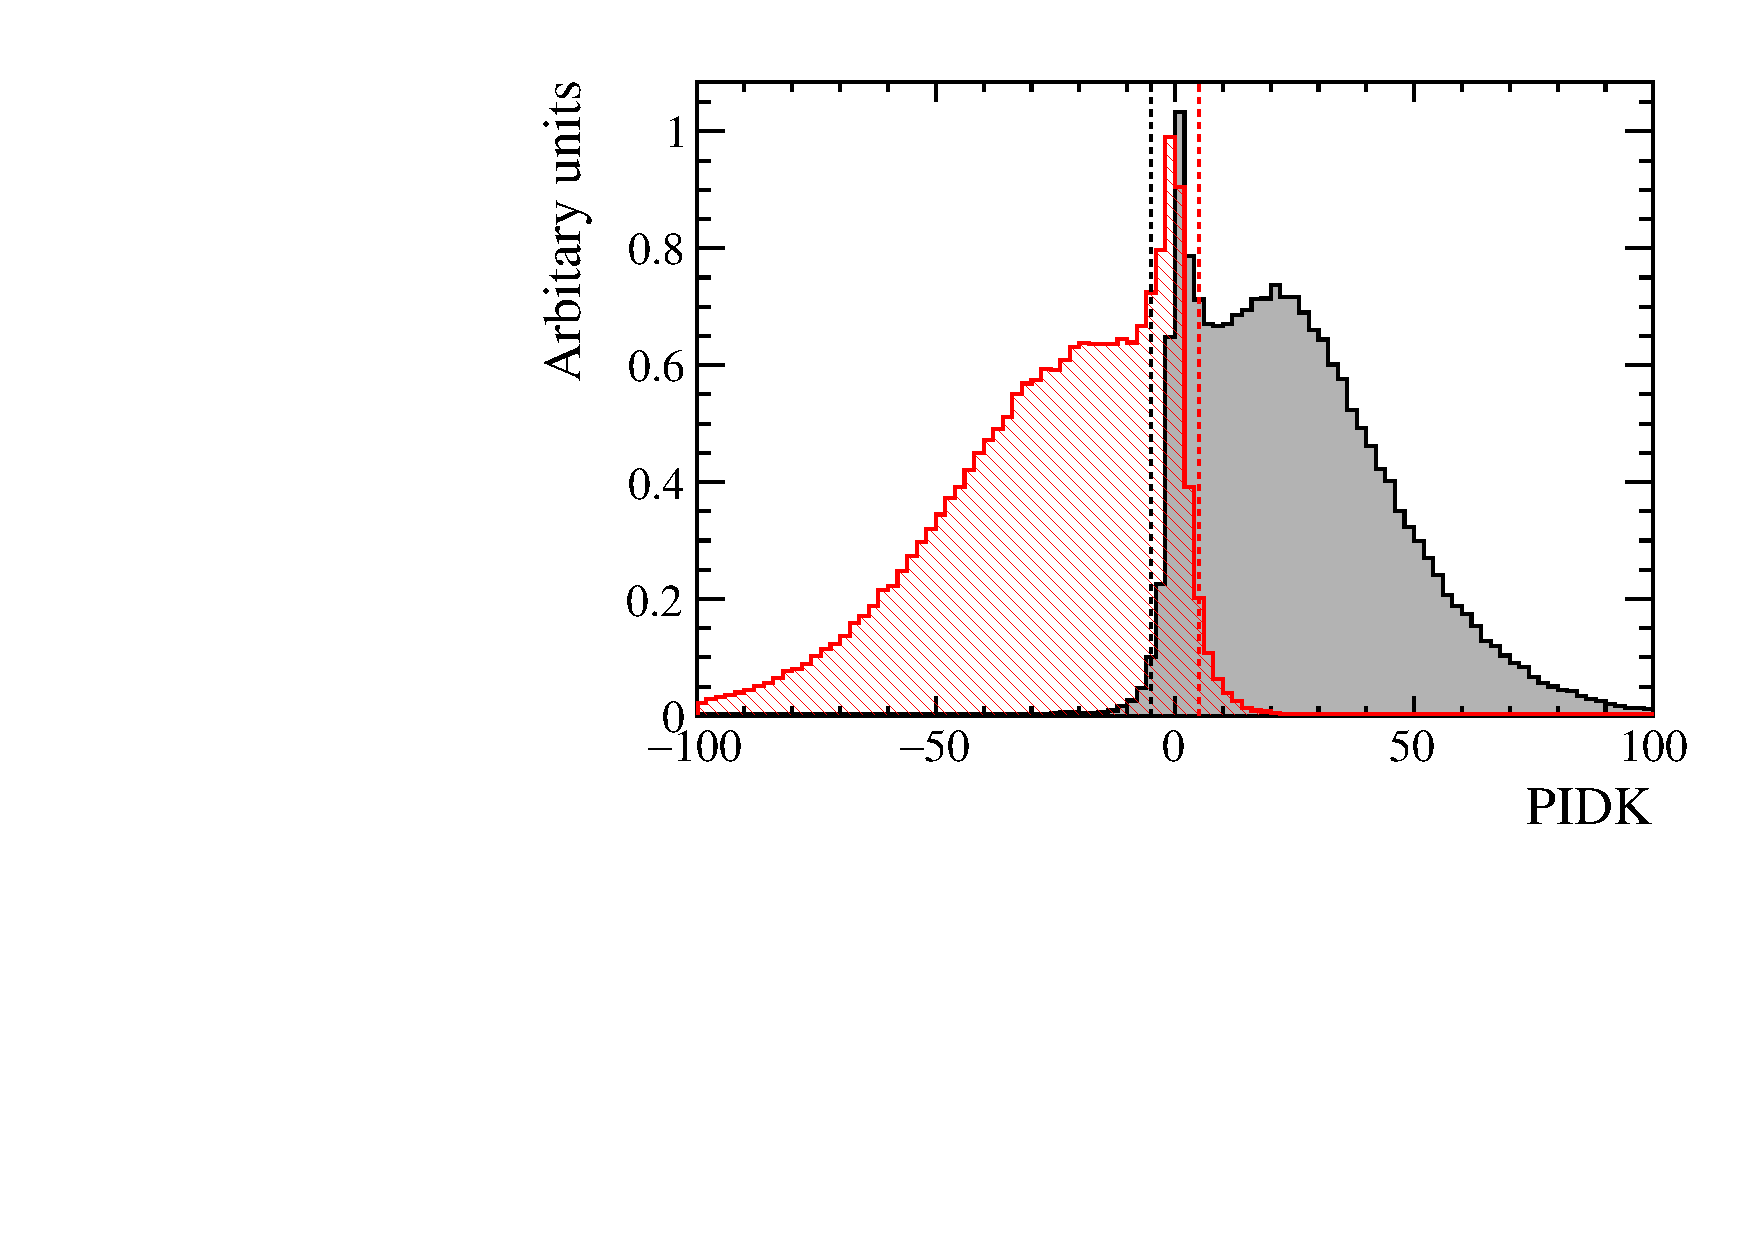
\includegraphics[width=0.6\textwidth]{figs/Selection/Calib_sample_PIDK.pdf}
        \caption{The distribution of the particle identification variable PIDK for pions (red) and kaons (black) from data calibration samples. The vertical dashed lines illustrate the requirements $\text{PIDK}>5$ and $\text{PIDK}<-5$ applied to kaons and pions respectively.}
    \label{fig:selection_PIDK_distribution}   
\end{figure}
%%%%%%%%%%%%%%%%%%%%%%%%%%%%%%%%%%%%%%%%%%%%%%%%%%%%%%%%%%





\subsection{Charmless and single-charm backgrounds}


Decays of \Bp mesons that didn't proceed via \D mesons could form a peaking background below the signal invariant mass distributions when they decay to the same final state.
The signal mode could receive contributions from the decays $\decay{\Bp}{h^{+}h^{-}h^{+}\phiz}$ or $\decay{\Bp}{h^{+}h^{-}h^{+}h^{+}h^{-}}$, referred to as charmless backgrounds. Here $h^{\pm}$ is used to represent \Kpm or \pipm in the specific \Dsp, \Dzb or \phiz final state.
The normalisation mode is also susceptible, however as it involves two charm mesons it could receive contributions from the decays $\decay{\Bp}{h^{+}h^{-}h^{+}\Dzb}$ or $\decay{\Bp}{\Dsp h^{+}h^{-}}$, referred to as single-charm backgrounds, and $\decay{\Bp}{h^{+}h^{-}h^{+} h^{+}h^{-}}$ referred to as a charmless background.
These backgrounds can be suppressed by requiring the \D meson decay vertex to be displaced from the \Bp meson decay vertex. Requirements are applied to the significance of the vertex separation ($\chi^{2}_{\text{FD}}$).

The residual yields of charmless backgrounds in the signal mode are estimated by performing a fit to the \Bp invariant mass for candidates with $25 < |m(h^{+}h^{-}h^{+}) - m(\Dsp)| < 50\mevcc $. This background estimation is performed separately for the \decay{\Bp}{\Dsp\phiz} and \decay{\Bp}{\Dsp\Kp\Km} searches. 

For the \decay{\Bp}{\Dsp\Dzb} normalisation channel, a two-dimensional optimisation is performed to calculate the contribution from decays without a \Dsp meson, \Dzb meson or both. 
The two-dimensional space defined by the \Dsp and \Dzb masses is split into four types of area as shown in Fig~\ref{fig:2d_normalisation}.

%%%%%%%%%%%%%%%%%%%%%%%%%%%%%%%%%%%%%%%%%%%%%%%%%%%%%%%%%%
\begin{figure}[!h]
    \centering
        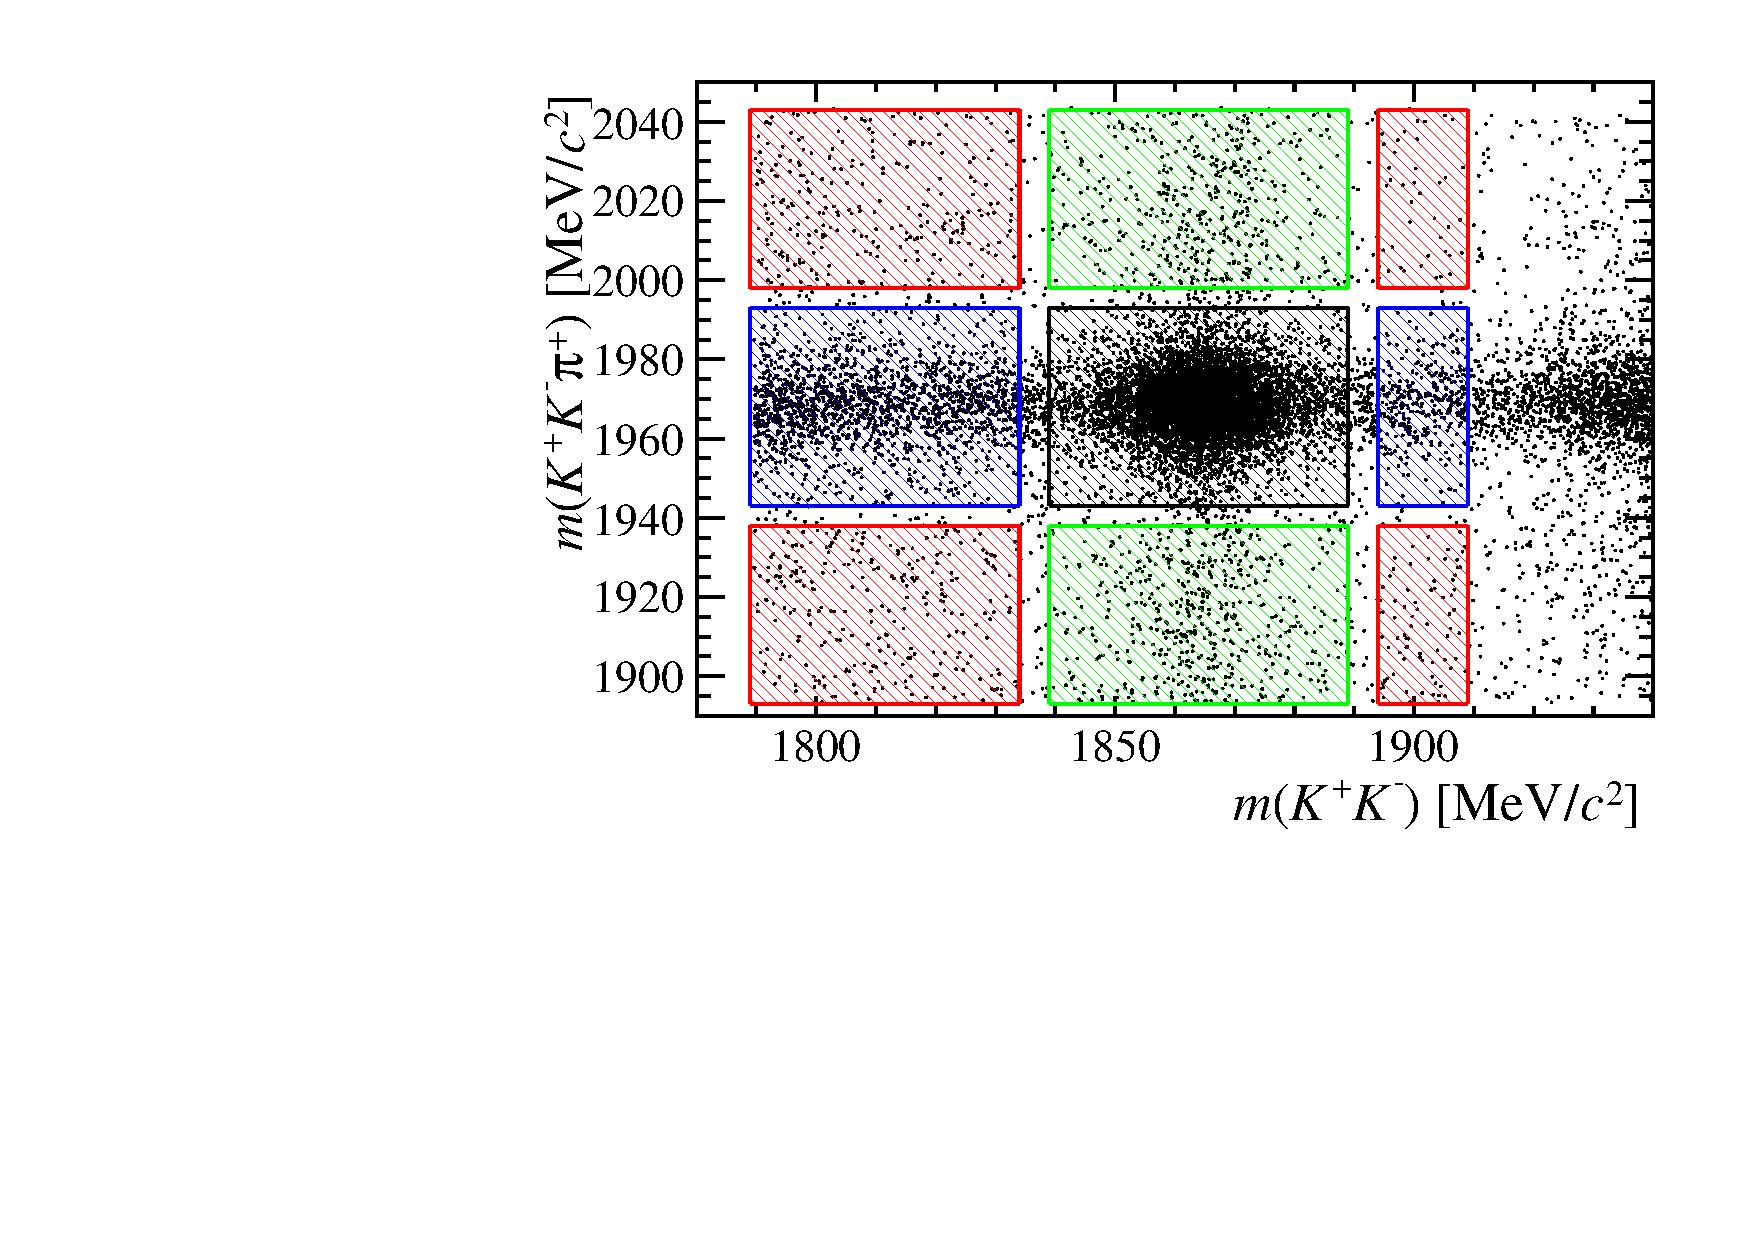
\includegraphics[width=0.6\textwidth]{figs/Selection/B2DsD0_2D_mass_Ds2KKPiRun2.pdf}
        \caption{Candidate \decay{\Bp}{\Dsp\Dzb} decays plotted as a function of the \Dsp and \Dzb invariant mass. The four regions described in the text are highlighted.}
    \label{fig:2d_normalisation}   
\end{figure}
%%%%%%%%%%%%%%%%%%%%%%%%%%%%%%%%%%%%%%%%%%%%%%%%%%%%%%%%%%

\begin{enumerate}
\item Areas in which only $\decay{\Bp}{h^{+}h^{-}h^{+}h^{+}h^{-}}$ decays contribute (red).
\item Areas in which either $\decay{\Bp}{D_{s}^{+}h^{+}h^{-}}$  or $\decay{\Bp}{h^{+}h^{-}h^{+} h^{+}h^{-}}$ decays can contribute (blue). 

\item Areas in which either $\decay{\Bp}{h^{+}h^{-}h^{+}\Dzb}$ or $\decay{\Bp}{h^{+}h^{-}h^{+} h^{+}h^{-}}$ decays can contribute (green). 
\item The signal region in which $\decay{\Bp}{D_{s}^{+} \Dzb}$, $\decay{\Bp}{h^{+}h^{-}h^{+}\Dzb}$, $\decay{\Bp}{D_{s}^{+}h^{+}h^{-}}$ or $\decay{\Bp}{h^{+}h^{-}h^{+}h^{+}h^{-}}$ decays could contribute (black).
\end{enumerate}   

Asymmetric \Dzb sidebands are used to prevent misidentified \decay{\Bp}{\Dsp (\decay{\Dzb}{\Km\pip})} decays from being included in the sideband sample.
The optimal selection requirements are chosen such that the maximal signal efficiency is achieved for a residual charmless contribution of $<2\%$ of the normalisation yield.

The optimisation of the signal and normalisation cuts is performed separately for each different \Dsp decay mode, and for the \decay{\Bp}{\Dsp\Kp\Km} and \decay{\Bp}{\Dsp\phiz} selections. The optimised requirements are listed in Table~\ref{tab:selection_fd_cuts}, along with the estimated residual yields of charmless and single charm yields in the signal region.  


\begin{table}[h]
   \centering
      \begin{tabular}{l c c c c }
         \hline
         \Bp decay mode         & \Dsp decay mode             & $\chi^{2}_{\text{FD}}(\Dsp)$  & $\chi^{2}_{\text{FD}}(\Dzb)$  & Residual yields \\ 
         \hline
         \decay{\Bp}{\Dsp\phiz} & \decay{\Dsp}{\Kp\Km\pip}    &  0.0              & -                 & 0.0             \\
         \decay{\Bp}{\Dsp\phiz} & \decay{\Dsp}{\Kp\pim\pip}   &  25.0             & -                 & 2.6             \\
         \decay{\Bp}{\Dsp\phiz} & \decay{\Dsp}{\pip\pim\pip}  &  5.0              & -                 & 0.0             \\
         \decay{\Bp}{\Dsp\Dzb}  & \decay{\Dsp}{\Kp\Km\pip}    &  8.0              & 0.0               & 21.6            \\
         \decay{\Bp}{\Dsp\Dzb}  & \decay{\Dsp}{\Kp\pim\pip}   &  18.0             & 0.0               & 3.3             \\
         \decay{\Bp}{\Dsp\Dzb}  & \decay{\Dsp}{\pip\pim\pip}  &  16.0             & 0.0               & 3.9             \\
         \hline
         \decay{\Bp}{\Dsp\Kp\Km} & \decay{\Dsp}{\Kp\Km\pip}   & 5.0               & -                 & 0.19            \\
         \decay{\Bp}{\Dsp\Dzb}   & \decay{\Dsp}{\Kp\Km\pip}   & 8.0               & 0.0               & 7.95            \\
         \hline
      \end{tabular}
   
   \caption{Charmless and single charm minimum flight distance significance requirements applied to the \Dsp and \Dzb candidates.}
   \label{tab:selection_fd_cuts}
\end{table}



\subsection{Misidentified \D and \Lc hadrons}
\label{sec:pidvetos}

It is possible for the samples \Dsp mesons to be contaminated by other misidentified decays of \Dp mesons or \Lc baryons in which one of the decay products has been incorrectly identified.
Such backgrounds can be vetoed by recalculating the invariant mass of the \Dsp meson, swapping the mass hypothesis of the ambiguous track to that of the \kaon, \pion or \proton, depending on the decay mode. 
The particle identification requirements are tightened within a mass window around the \Dp or \Lc mass, effectively removing this crossfeed. For the mode \decay{\Dsp}{\Kp\Km\pip}, the vetoes are not applied to candidates for which $m|(\Km\Kp)-m_{\phiz}| < 10\mevcc$ as there are a high purity of \decay{\Dsp}{\Kp\Km\pip} decays in this region.

The specific vetoes included in this selection are listed in Table~\ref{table:pidvetos}. 
\begin{table*}[!ht]
\centering
\begin{tabular}{ l l l }
\hline
Decay Mode & Misidentified decay\\
\hline
\decay{\Dsp}{{\color{Red}\Kp}\Km\pip}   & \decay{\Dp}{{\color{Red}\pip}\Km\pip}    \\
                           & \decay{\Lc}{{\color{Red}\Pp}\Km\pip}     \\
%                           &                             \\
\hline
\decay{\Dsp}{{\color{Red}\Kp}\pim\pip}  & \decay{\Dp}{{\color{Red}\pip}\pim\pip}   \\
%                           &                             \\

\hline
\end{tabular}
\caption{Misidentified decays targeted by vetoes. The ambiguous track is highlighted in red in each case.}
\label{table:pidvetos}

\end{table*}
The invariant mass distributions for each the misidentified \decay{\Dsp}{\Kp\Km\pip} decays are shown with and without the MVA requirements in Figs.~\ref{fig:PIDVetos_Ds2KKPi_D_Veto} and \ref{fig:PIDVetos_Ds2KKPi_Lc_Veto} for both the signal \decay{\Bp}{\Dsp\phiz} and normalisation \decay{\Bp}{\Dsp\Dzb} decays.



%%%%%%%%%%%%%%%%%%%%%%%%%%%%%%%%%%%%%%%%%%%%%%%%%%%%%%%%%%
\begin{figure}[!h]
    \centering
    \begin{subfigure}[t]{0.4\textwidth}
        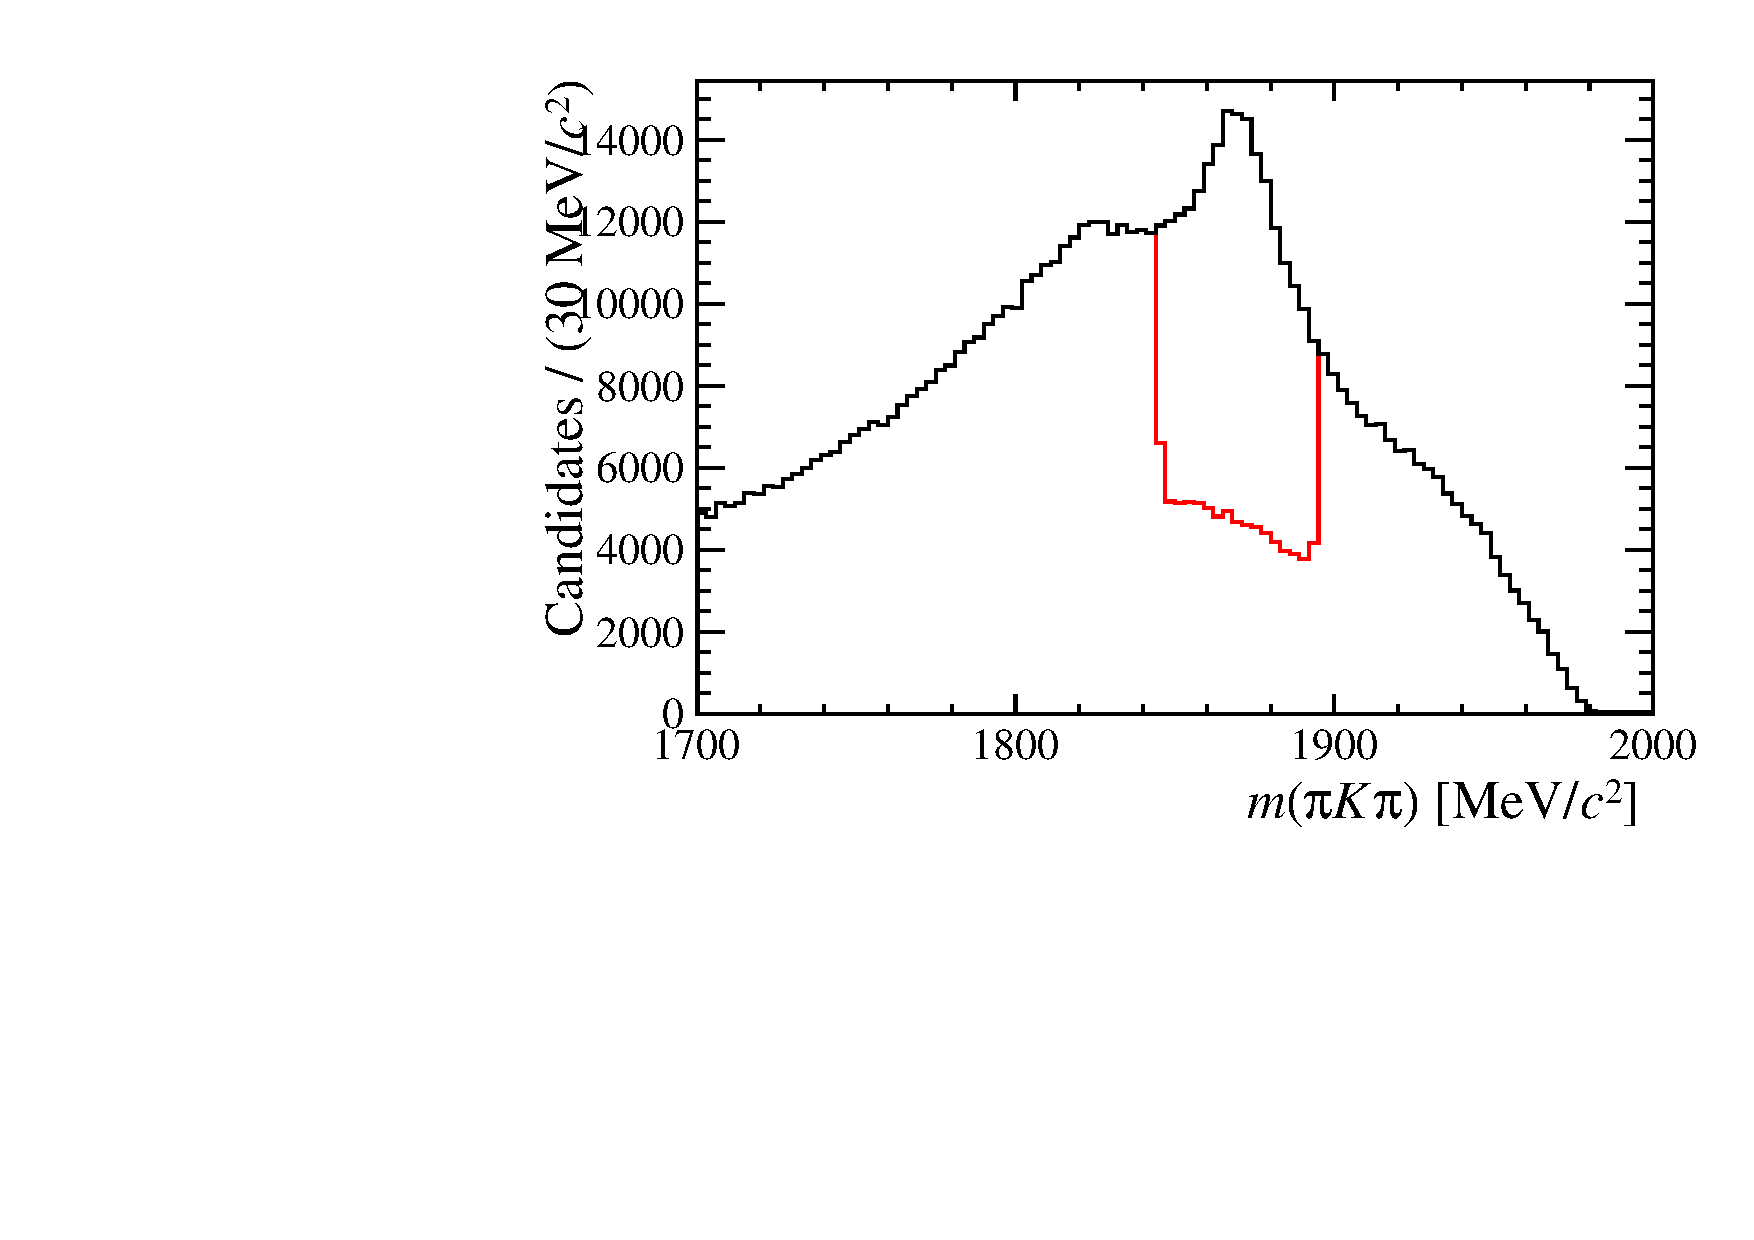
\includegraphics[width=1.0\textwidth]{figs/Selection/B2DsD0_Ds2KKPi_D_Veto_NoBDT.pdf}
        \caption{Normalisation without selection}
    \end{subfigure}%
    \begin{subfigure}[t]{0.4\textwidth}
        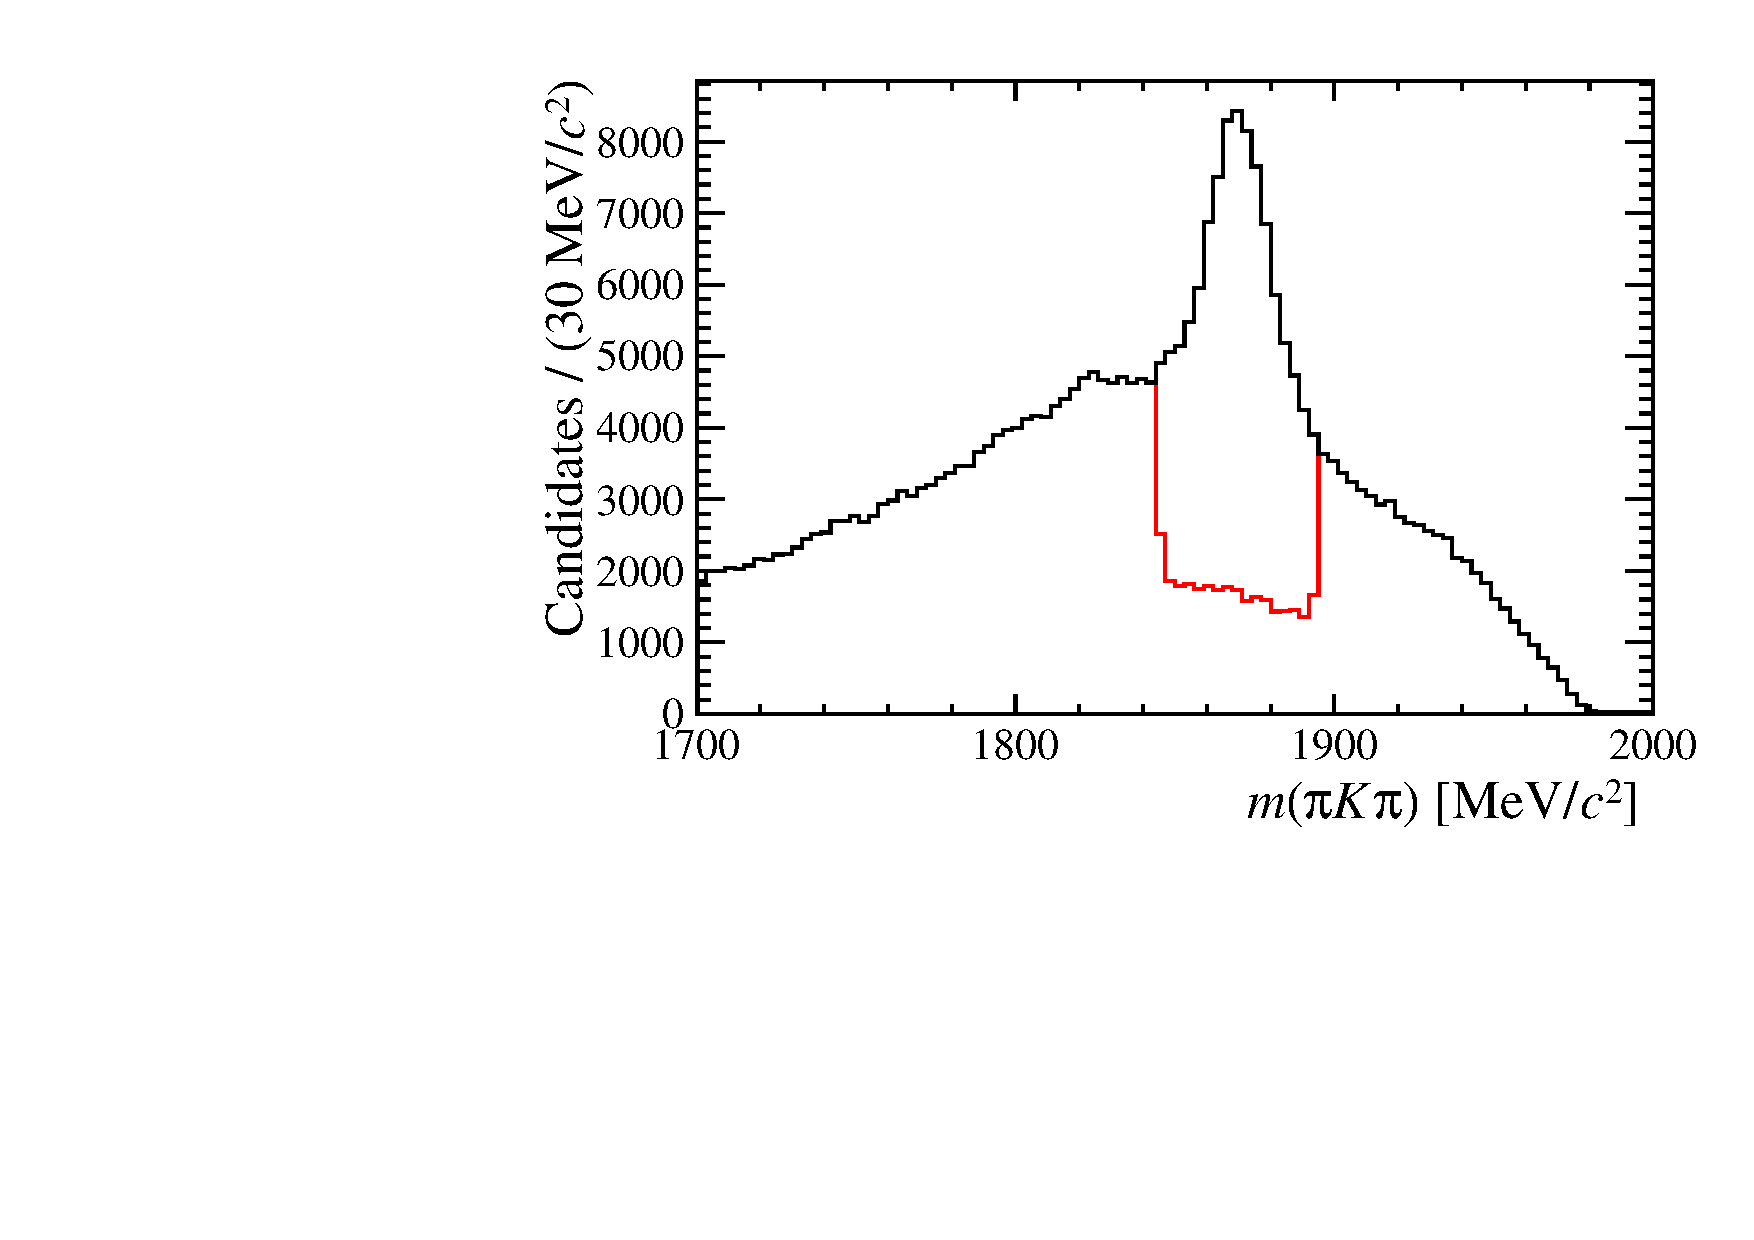
\includegraphics[width=1.0\textwidth]{figs/Selection/B2DsPhi_Ds2KKPi_D_Veto_NoBDT.pdf}
        \caption{Signal without selection}
    \end{subfigure}\\
    \begin{subfigure}[t]{0.4\textwidth}
        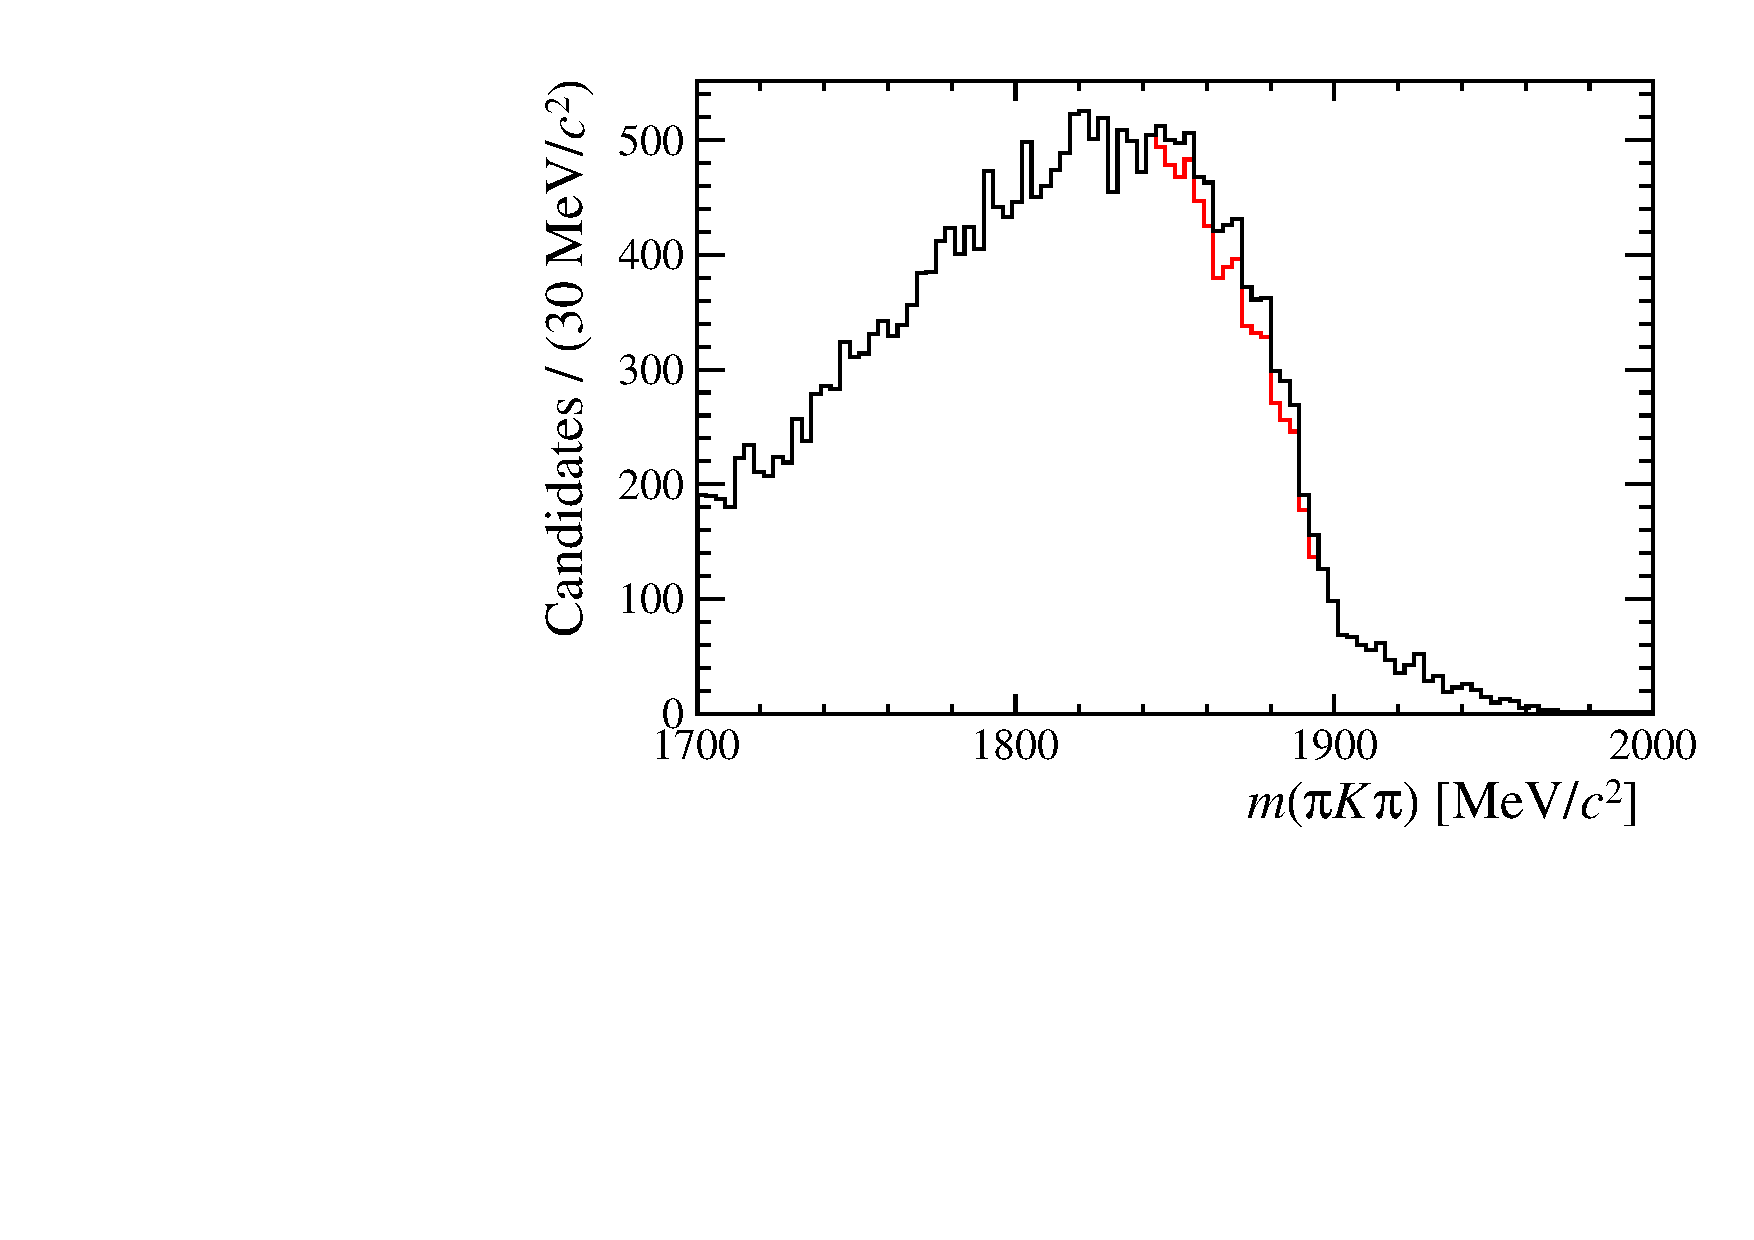
\includegraphics[width=1.0\textwidth]{figs/Selection/B2DsD0_Ds2KKPi_D_Veto_WithBDT.pdf}
        \caption{Normalisation with selection}
    \end{subfigure}%
    \begin{subfigure}[t]{0.4\textwidth}
        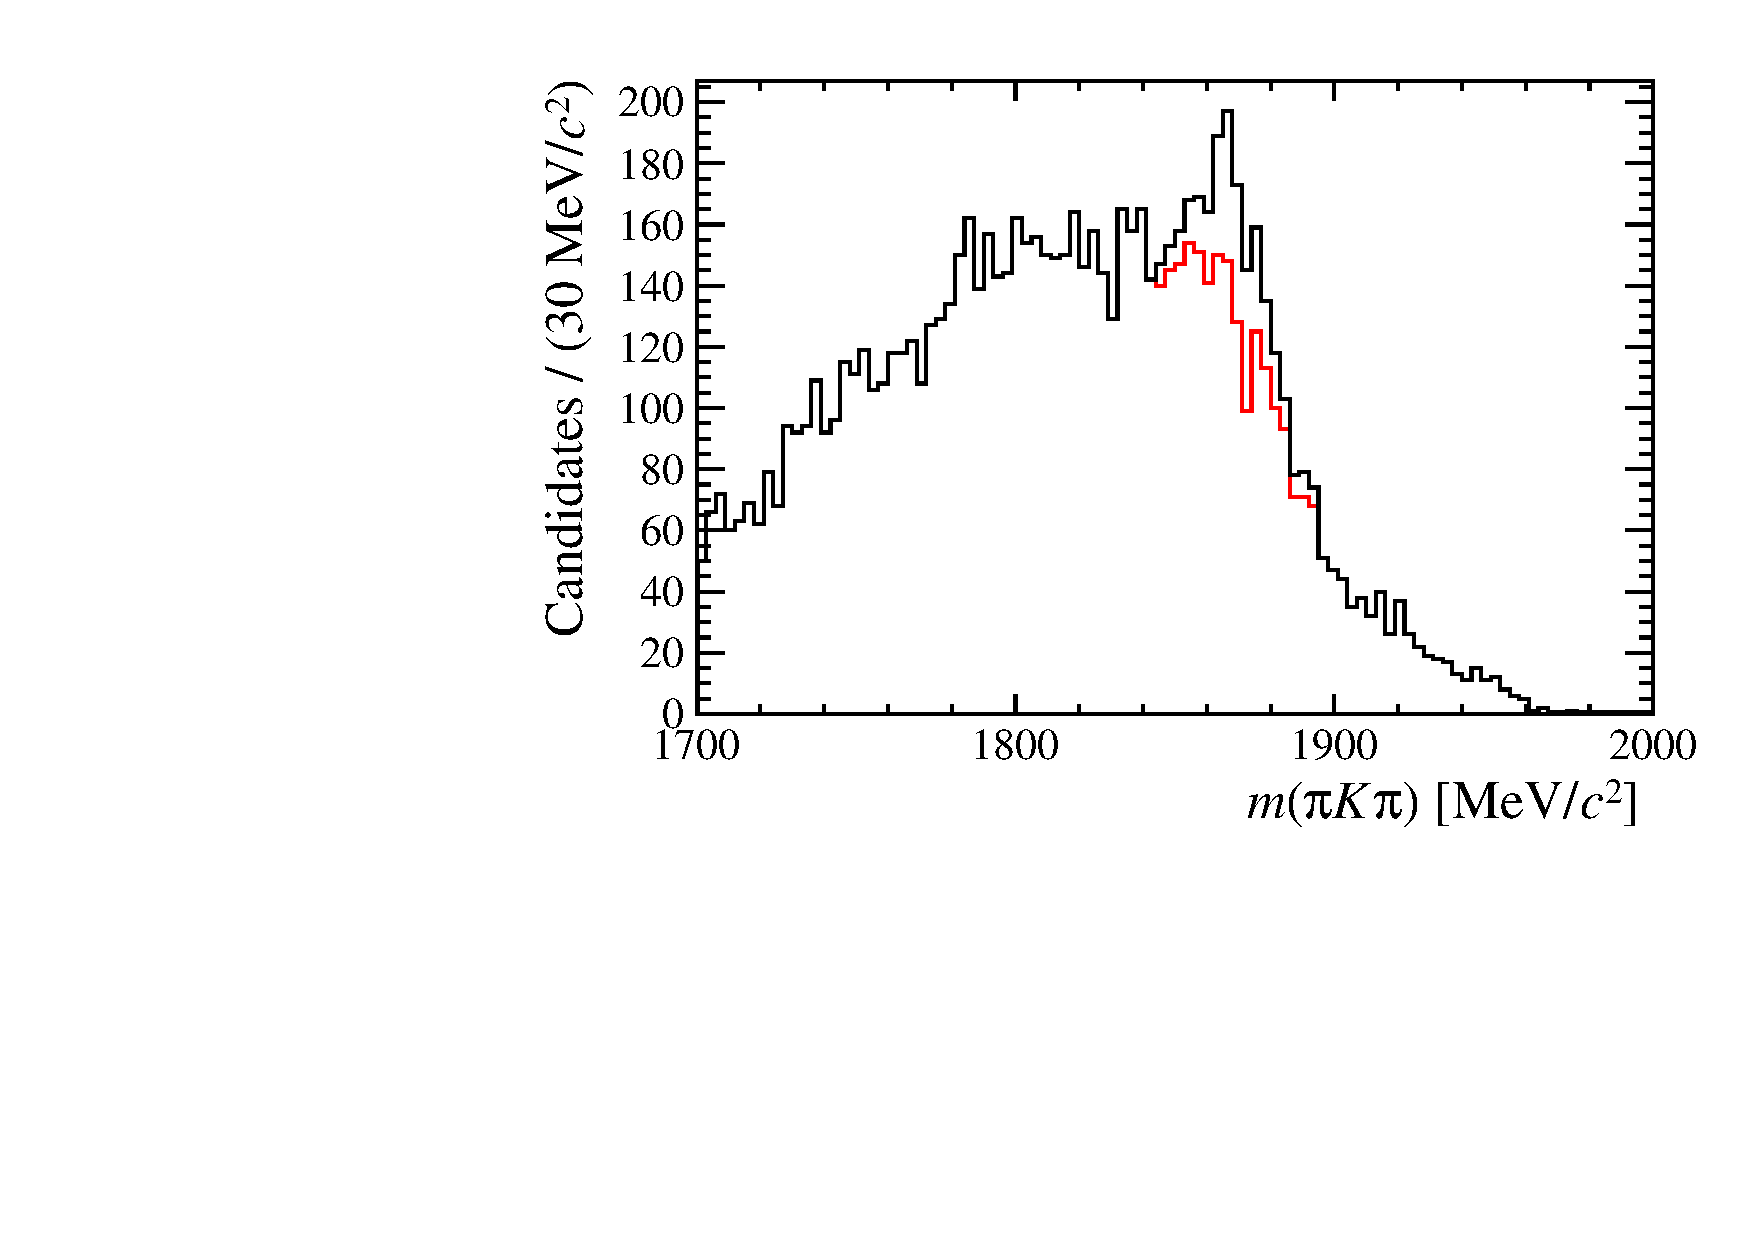
\includegraphics[width=1.0\textwidth]{figs/Selection/B2DsPhi_Ds2KKPi_D_Veto_WithBDT.pdf}
        \caption{Signal with selection}
    \end{subfigure}\\
    \caption{Invariant mass distributions of \decay{\Dsp}{\Kp\Km\pip} samples reconstructed as \decay{\Dp}{\pip\Km\pip} for the signal and normalisation samples. The samples are shown with (red) and without (black) the veto described in Sec.~\ref{sec:pidvetos}. The distributions are shown before (top) and after (bottom) the MVA requirements have been applied.}
    \label{fig:PIDVetos_Ds2KKPi_D_Veto}   
\end{figure}
%%%%%%%%%%%%%%%%%%%%%%%%%%%%%%%%%%%%%%%%%%%%%%%%%%%%%%%%%%

%%%%%%%%%%%%%%%%%%%%%%%%%%%%%%%%%%%%%%%%%%%%%%%%%%%%%%%%%%
\begin{figure}[!h]
    \centering
    \begin{subfigure}[t]{0.4\textwidth}
        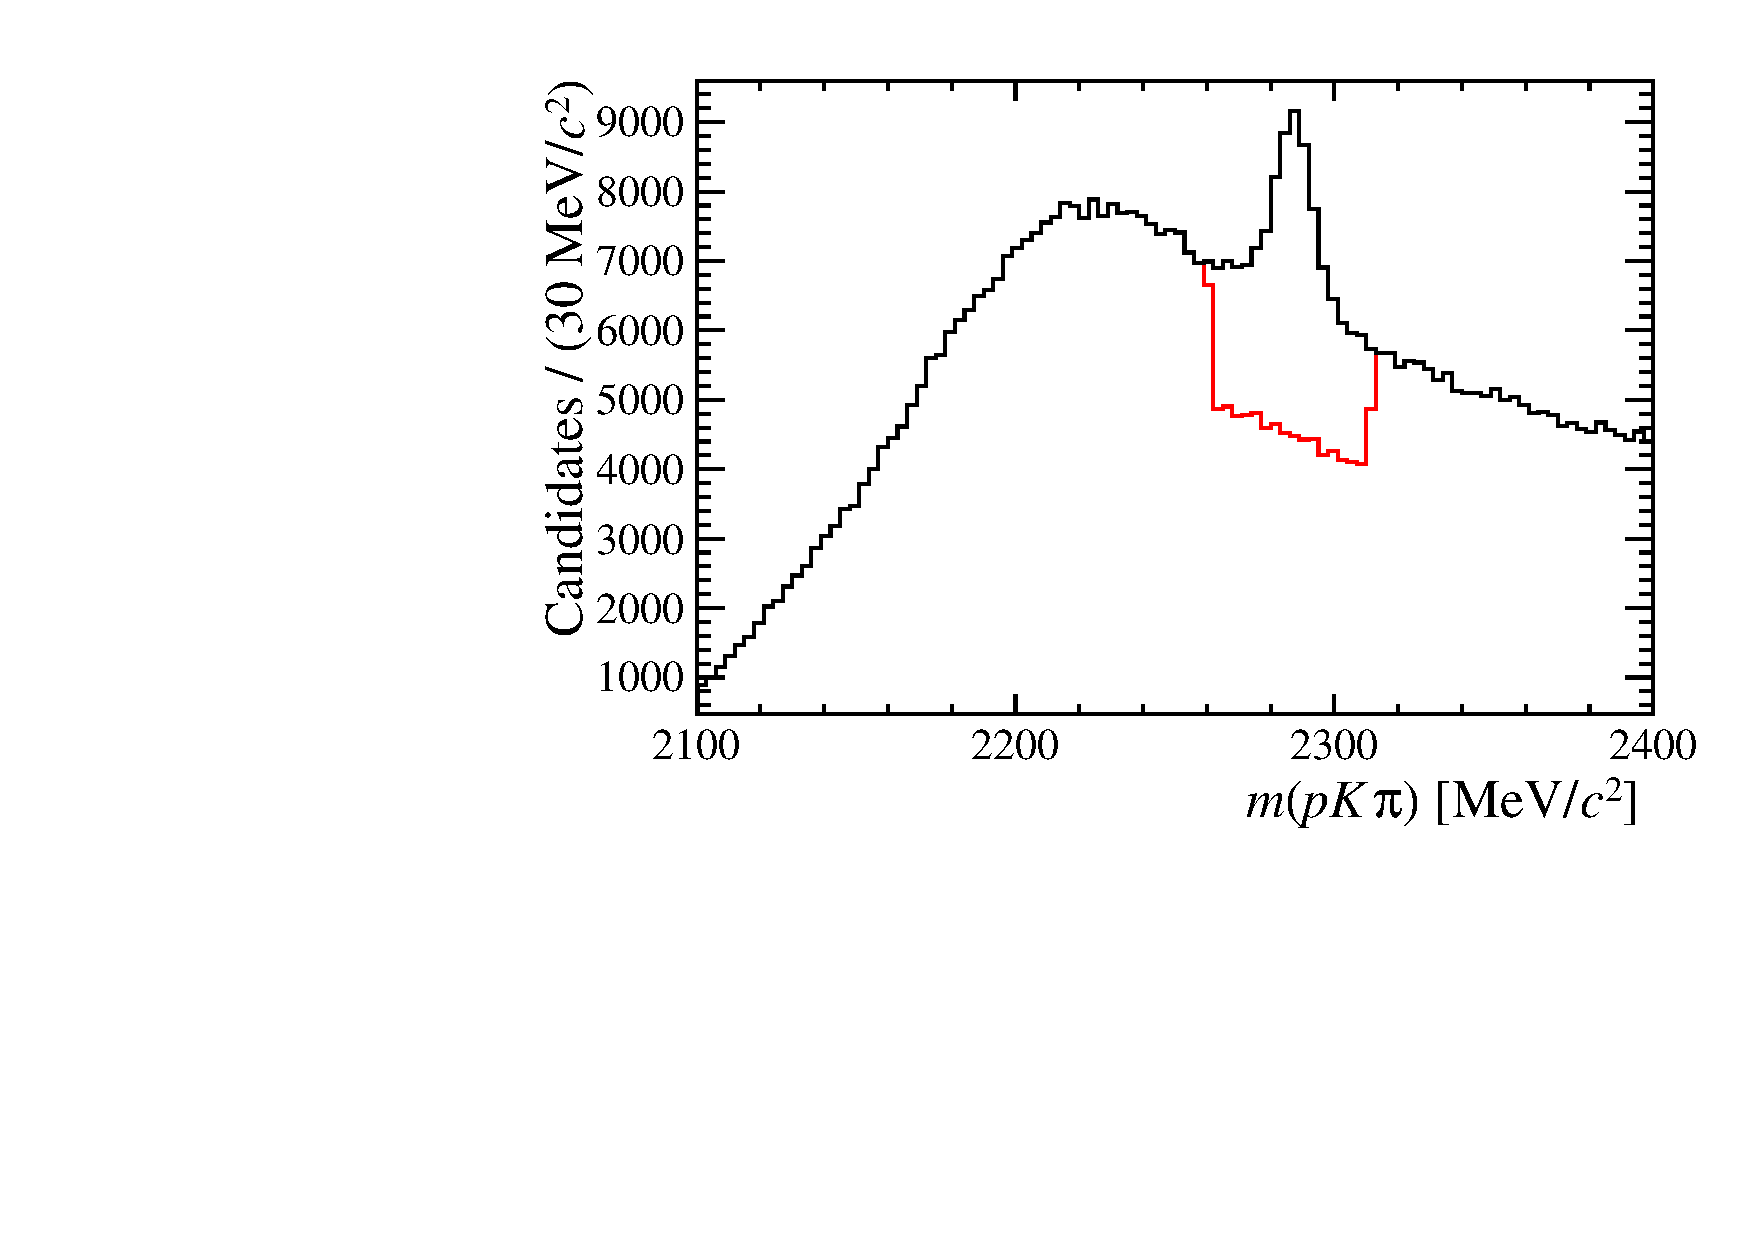
\includegraphics[width=1.0\textwidth]{figs/Selection/B2DsD0_Ds2KKPi_Lc_Veto_NoBDT.pdf}
        \caption{Normalisation without MVA cut}
    \end{subfigure}%
    \begin{subfigure}[t]{0.4\textwidth}
        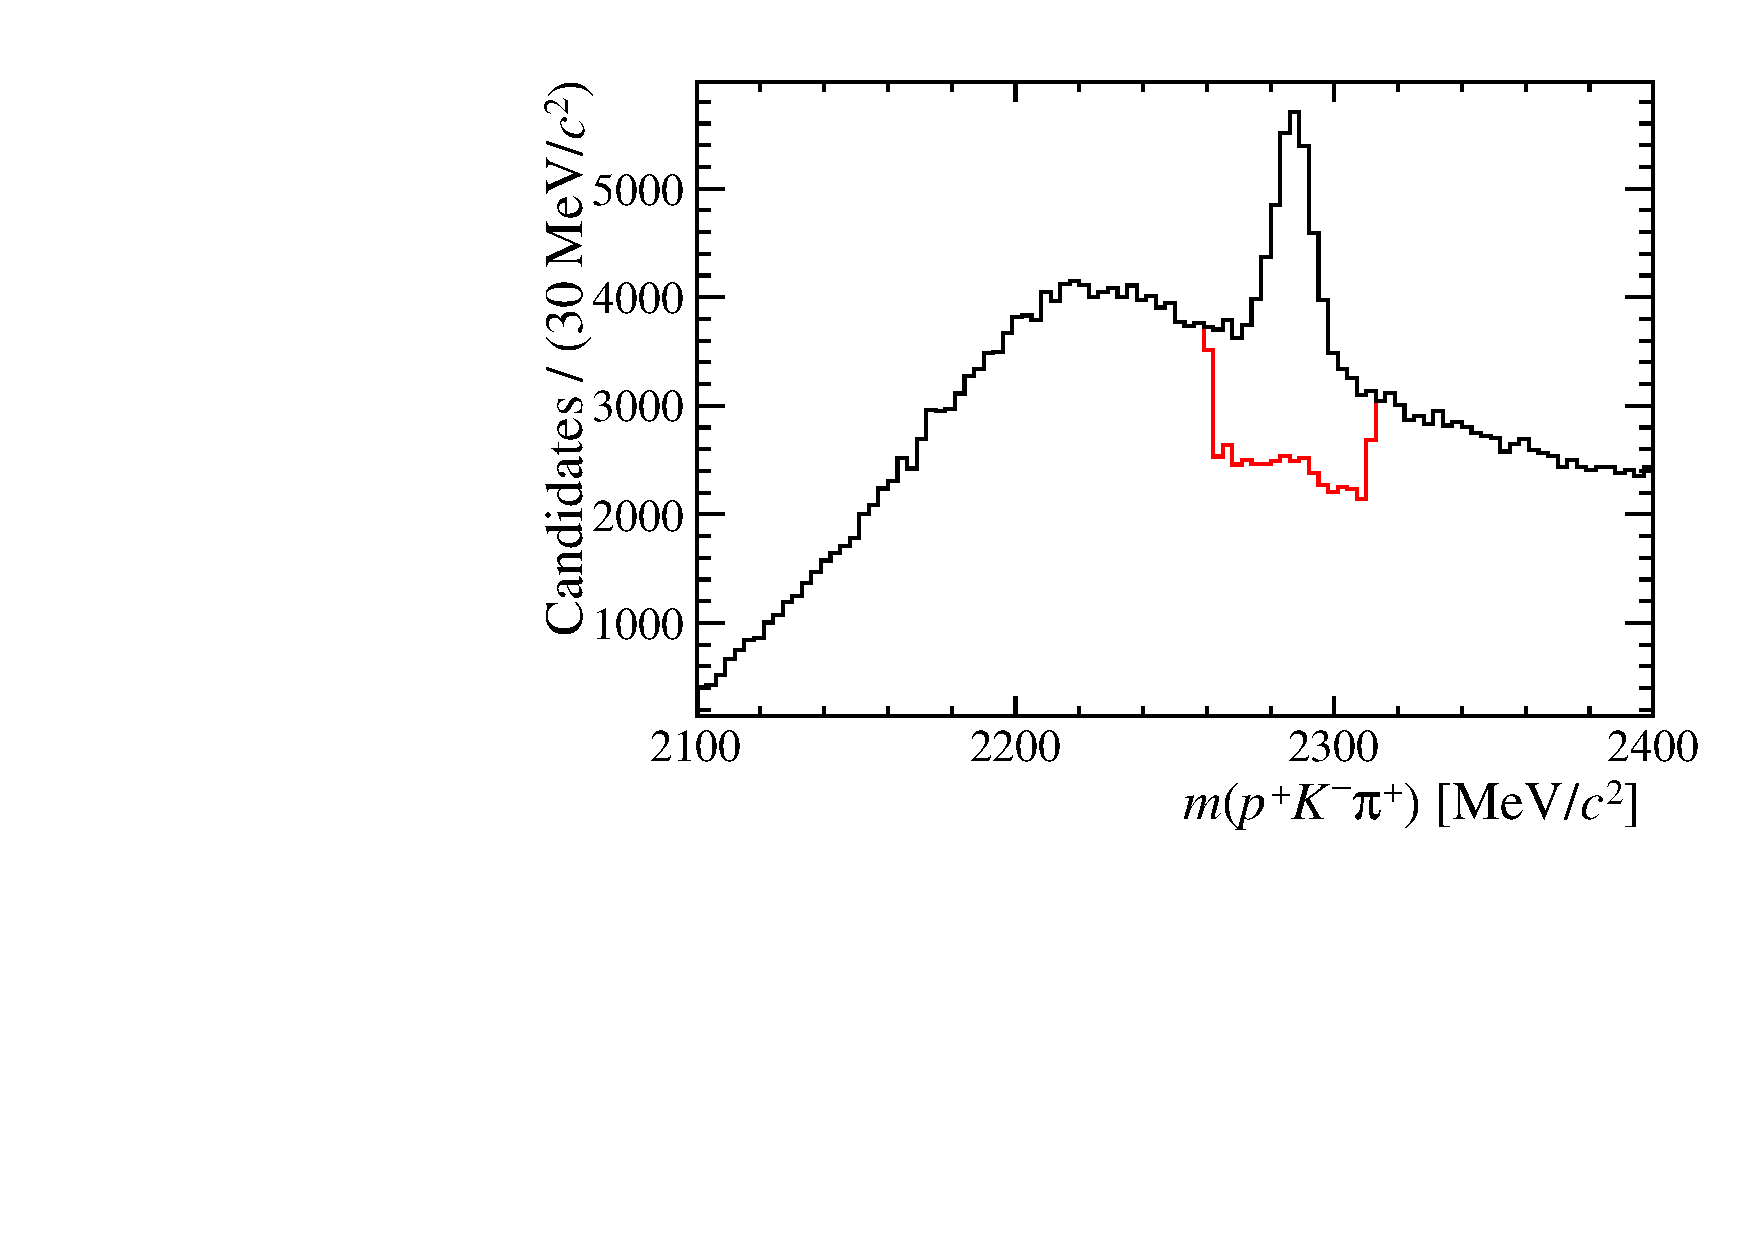
\includegraphics[width=1.0\textwidth]{figs/Selection/B2DsPhi_Ds2KKPi_Lc_Veto_NoBDT.pdf}
        \caption{Signal without MVA cut}
    \end{subfigure}\\
    \begin{subfigure}[t]{0.4\textwidth}
        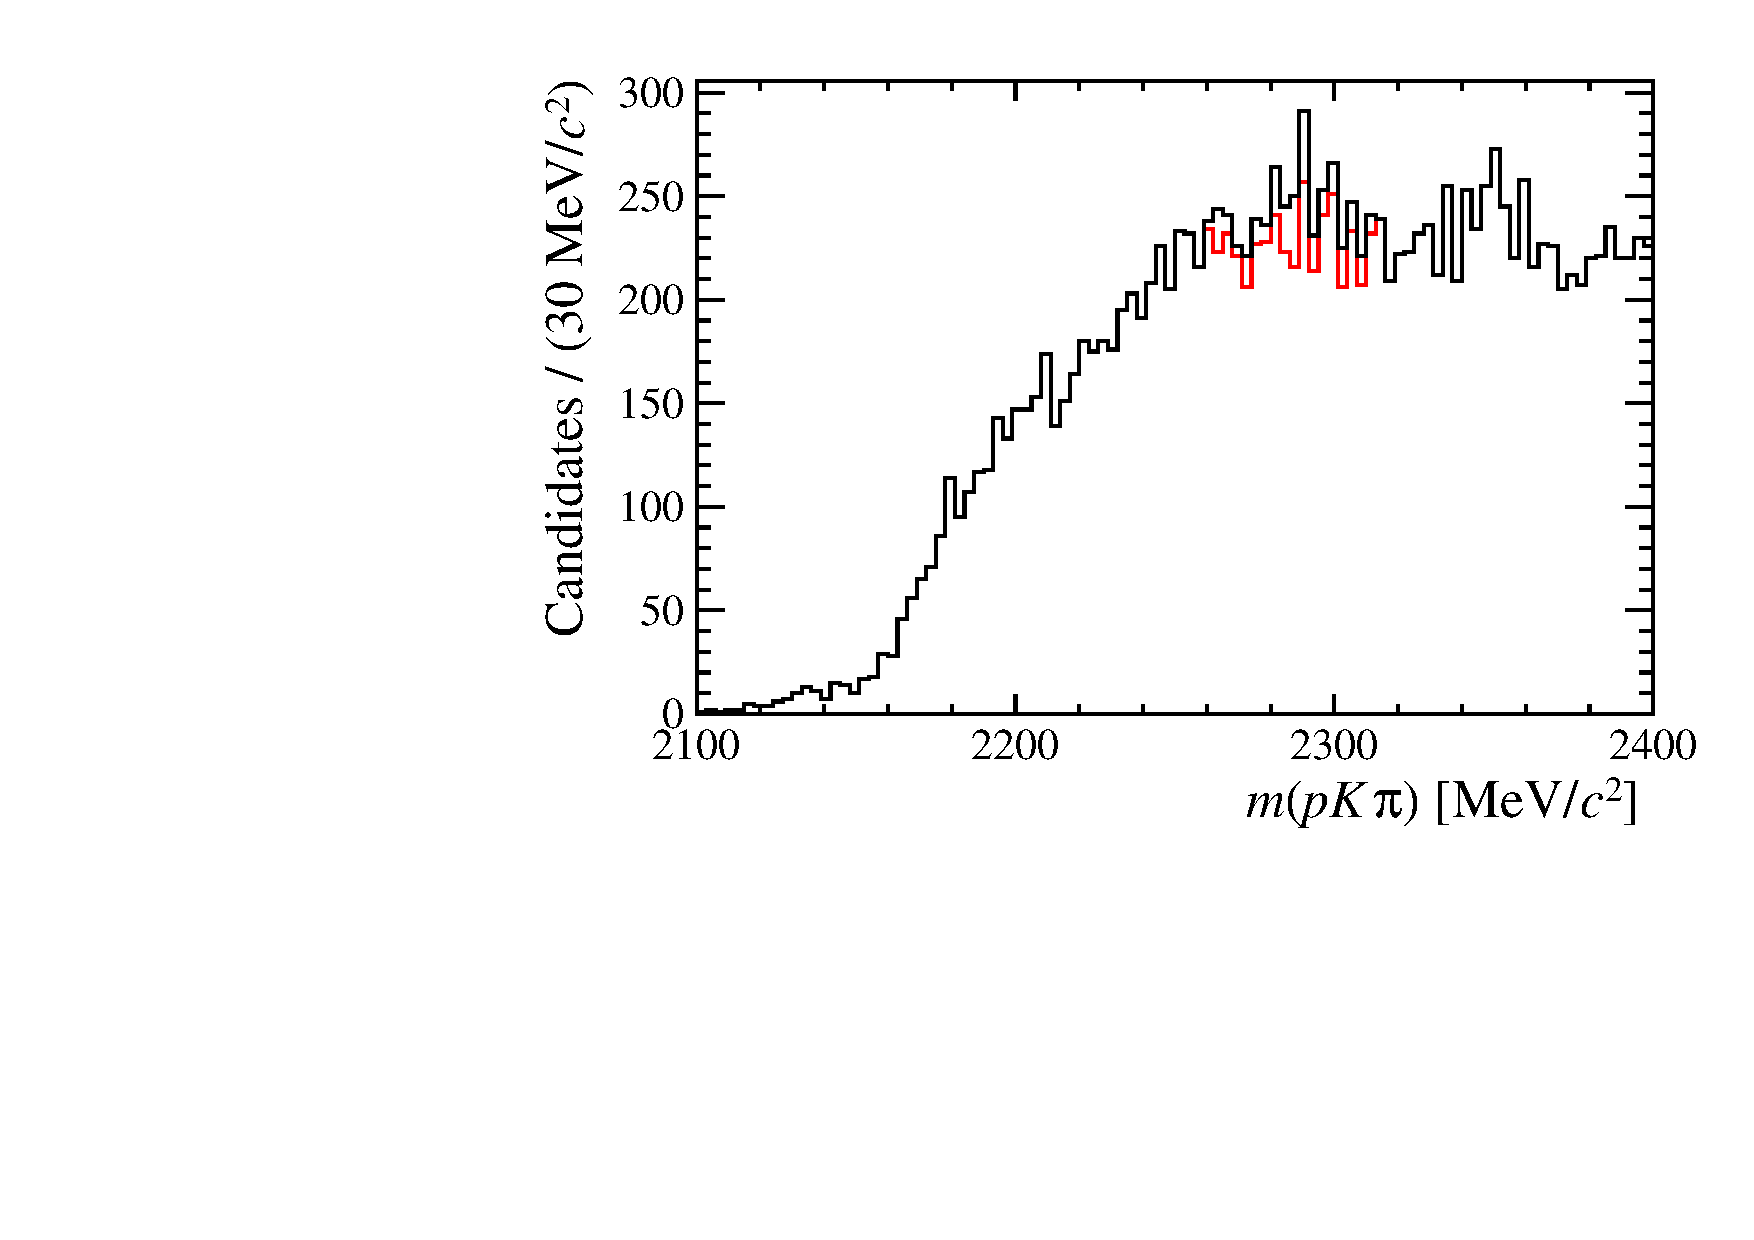
\includegraphics[width=1.0\textwidth]{figs/Selection/B2DsD0_Ds2KKPi_Lc_Veto_WithBDT.pdf}
        \caption{Normalisation with MVA cut}
    \end{subfigure}%
    \begin{subfigure}[t]{0.4\textwidth}
        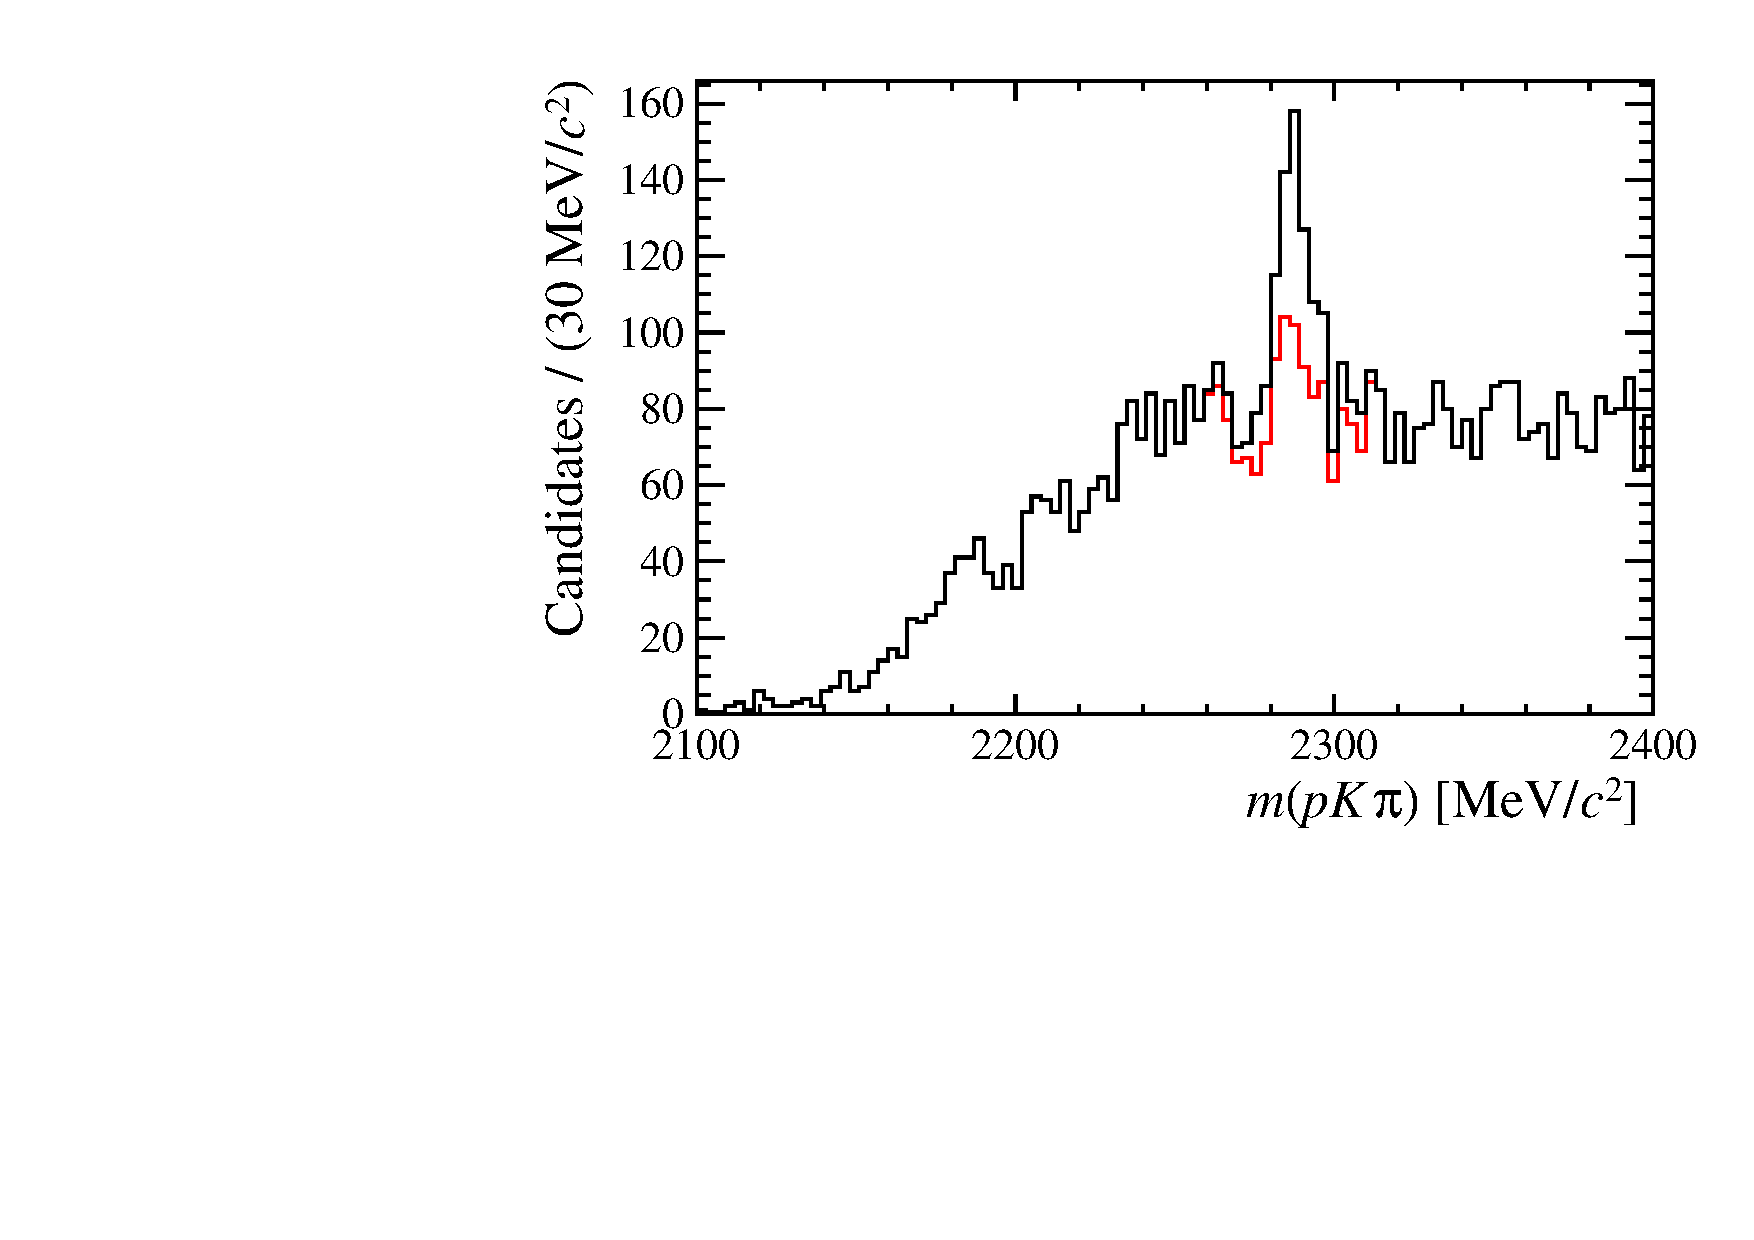
\includegraphics[width=1.0\textwidth]{figs/Selection/B2DsPhi_Ds2KKPi_Lc_Veto_WithBDT.pdf}
        \caption{Signal with MVA cut}
    \end{subfigure}\\
    \caption{Invariant mass distributions of \decay{\Dsp}{\Kp\Km\pip} samples reconstructed as \decay{\Lc}{\Pp\Km\pip} for the signal and normalisation samples. The samples are shown with (red) and without (black) the veto described in Sec.~\ref{sec:pidvetos}. The distributions are shown before (top) and after (bottom) the MVA requirements have been applied.}
    \label{fig:PIDVetos_Ds2KKPi_Lc_Veto}   
\end{figure}
%%%%%%%%%%%%%%%%%%%%%%%%%%%%%%%%%%%%%%%%%%%%%%%%%%%%%%%%%%

\subsection{Invariant mass vetoes}
\label{sec:kinematicvetos}

Sharp peaking structures are observed in subsets of the final state particles. These are removed with simple invariant mass cuts to remove combinatorial or partially reconstructed backgrounds that result from these incorrectly reconstructed decays. 
For simplicity the final state particles for each mode are labelled with a number between 1--5 as described in Table~\ref{table:vetolabels}.

\begin{table*}[!ht]
\centering
\begin{tabular}{ l c c c c c c }
\hline
Decay Mode & 1  & 2 & 3 & 4 & 5 \\
\hline
\decay{\Bp}{(\decay{\Dsp}{\Kp\Km\pip})\phiz}       & \Kp    & \Km    & \pip  & \Kp  & \Km \\
\decay{\Bp}{(\decay{\Dsp}{\pip\pim\pip})\phiz}     & \pip   & \pim   & \pip  & \Kp  & \Km \\
\decay{\Bp}{(\decay{\Dsp}{\Kp\pim\pip})\phiz}      & \Kp    & \pim   & \pip  & \Kp  & \Km \\
\hline
\decay{\Bp}{(\decay{\Dsp}{\Kp\Km\pip})\Kp\Km}      & \Kp    & \Km    & \pip  & \Kp  & \Km \\
\hline
\end{tabular}
\caption{Particle labels used when studying invariant mass vetoes for \decay{\Bp}{\Dsp\phiz} and \decay{\Bp}{\Dsp\Kp\Km} candidates.}
\label{table:vetolabels}

\end{table*}

All combinations of the final state particles that create a neutral or singly-charged candidate are investigated.
Significant structures are observed for all three \Dsp decay modes in some combination. 

The following vetos are applied to remove these incorrectly reconstructed decays.
\begin{itemize}
\item For the mode \decay{\Bp}{(\decay{\Dsp}{\Kp\Km\pip})\phiz}
\begin{itemize}
\item $|m(\text{1245})- m(\Bs)| > 50\mevcc$
\item $|m(\text{345})- m(\Dsp)| > 25\mevcc$ and $|m(\text{345})- m(\Dp)| > 25\mevcc$
\end{itemize}

\item For the mode \decay{\Bp}{(\decay{\Dsp}{\pip\pim\pip})\phiz}
\begin{itemize}
\item $|m(\text{145})- m(\Dsp)| > 25\mevcc$ and $|m(\text{145})- m(\Dp)| > 25\mevcc$
\item $|m(\text{245})- m(\Dsp)| > 25\mevcc$ and $|m(\text{245})- m(\Dp)| > 25\mevcc$
\item $|m(\text{345})- m(\Dsp)| > 25\mevcc$ and $|m(\text{345})- m(\Dp)| > 25\mevcc$
\end{itemize}
\item For the mode \decay{\Bp}{(\decay{\Dsp}{\Kp\pim\pip})\phiz}
\begin{itemize}
\item $|m(\text{245})- m(\Dsp)| > 25\mevcc$ and $|m(\text{245})- m(\Dp)| > 25\mevcc$
\item $|m(\text{345})- m(\Dsp)| > 25\mevcc$ and $|m(\text{345})- m(\Dp)| > 25\mevcc$
\end{itemize}
\end{itemize}

%%%%%%%%%%%%%%%%%%%%%%%%%%%%%%%%%%%%%%%%%%%%%%%%%%%%%%%%%%
\begin{figure}[!h]
   \centering
   \begin{subfigure}[t]{1.0\textwidth}
      \centering
      \begin{subfigure}[t]{0.32\textwidth}
         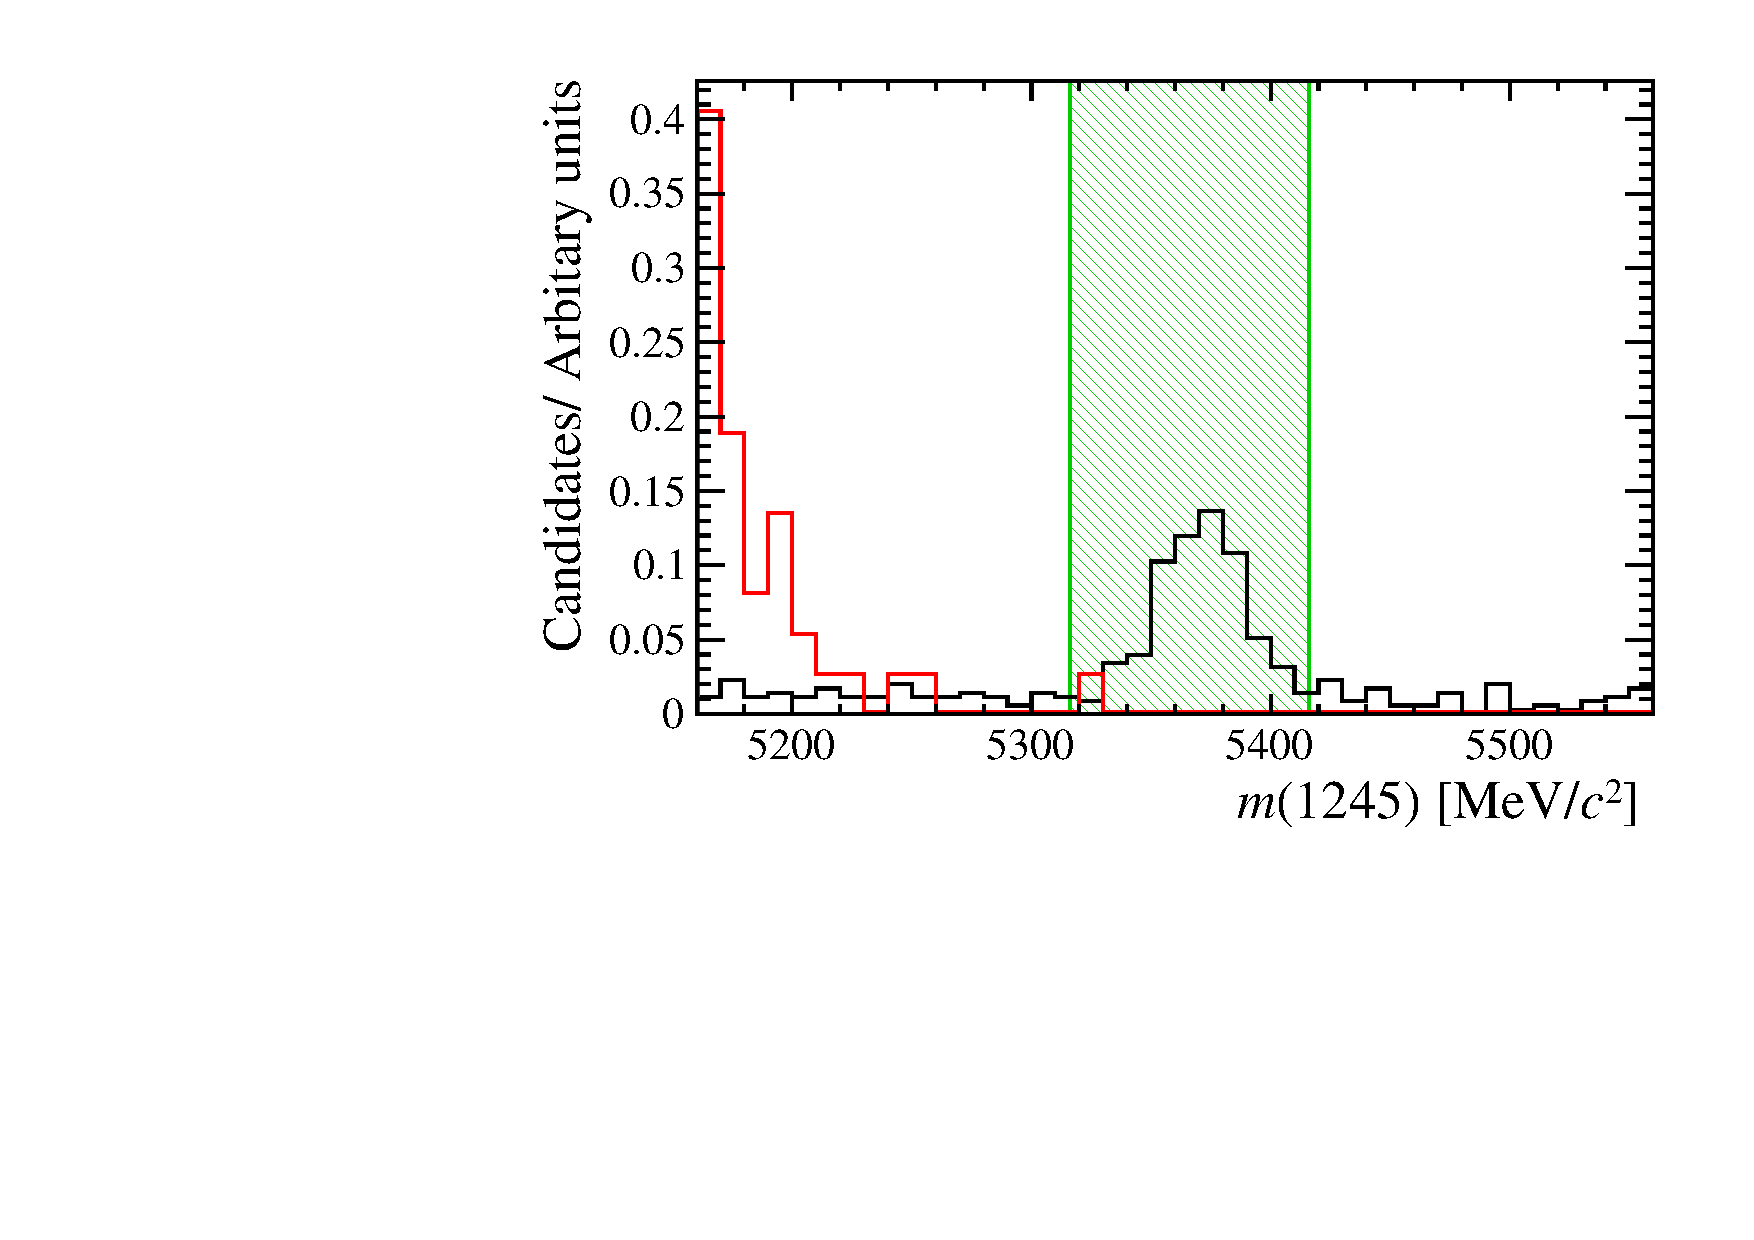
\includegraphics[width=1.0\textwidth]{figs/Selection/Veto_Comparison_B2DsPhi_Ds2KKPi_m1245.pdf}
      \end{subfigure}
      \begin{subfigure}[t]{0.32\textwidth}
         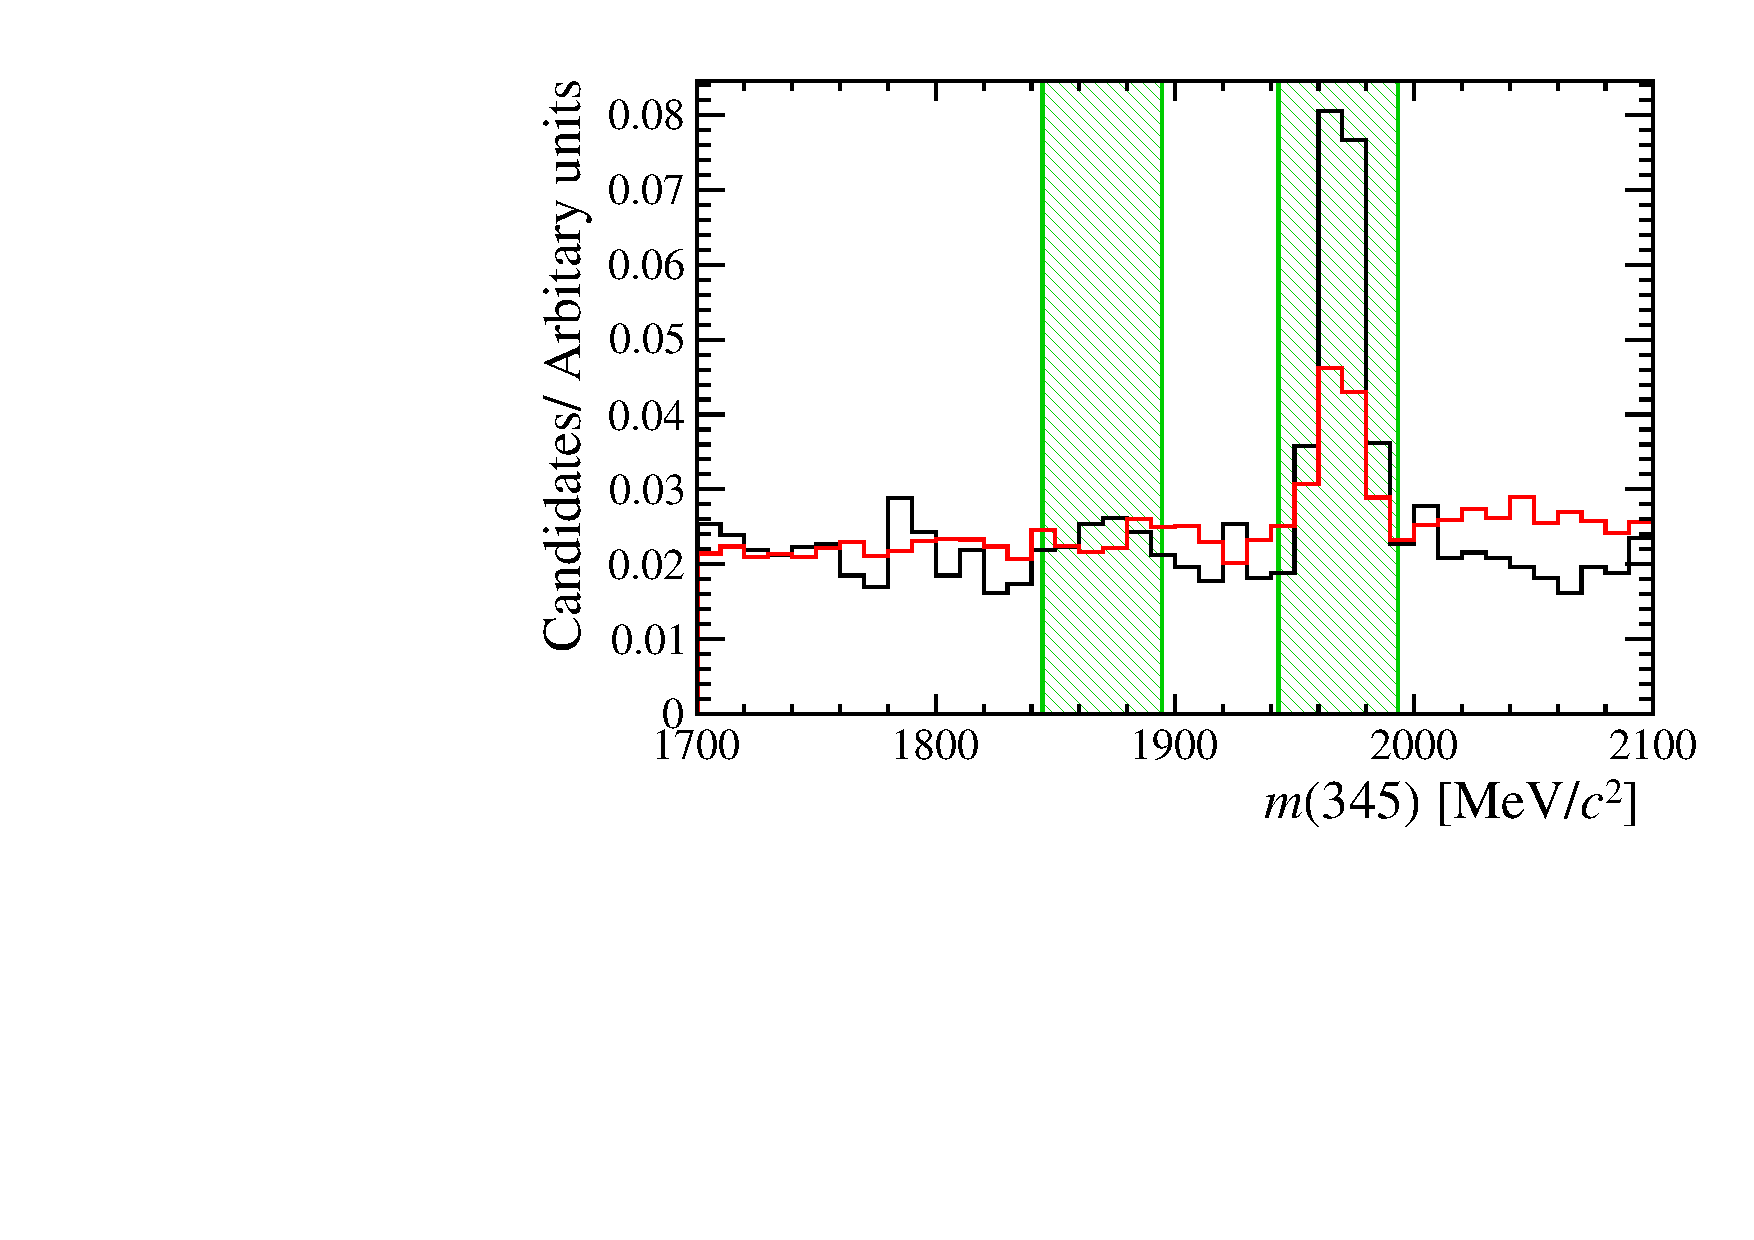
\includegraphics[width=1.0\textwidth]{figs/Selection/Veto_Comparison_B2DsPhi_Ds2KKPi_m345.pdf}
      \end{subfigure}
      \caption{\decay{\Bp}{(\decay{\Dsp}{\Kp\Km\pip})\phiz}}
   \end{subfigure}
   \begin{subfigure}[t]{1.0\textwidth}
      \centering
      \begin{subfigure}[t]{0.32\textwidth}
         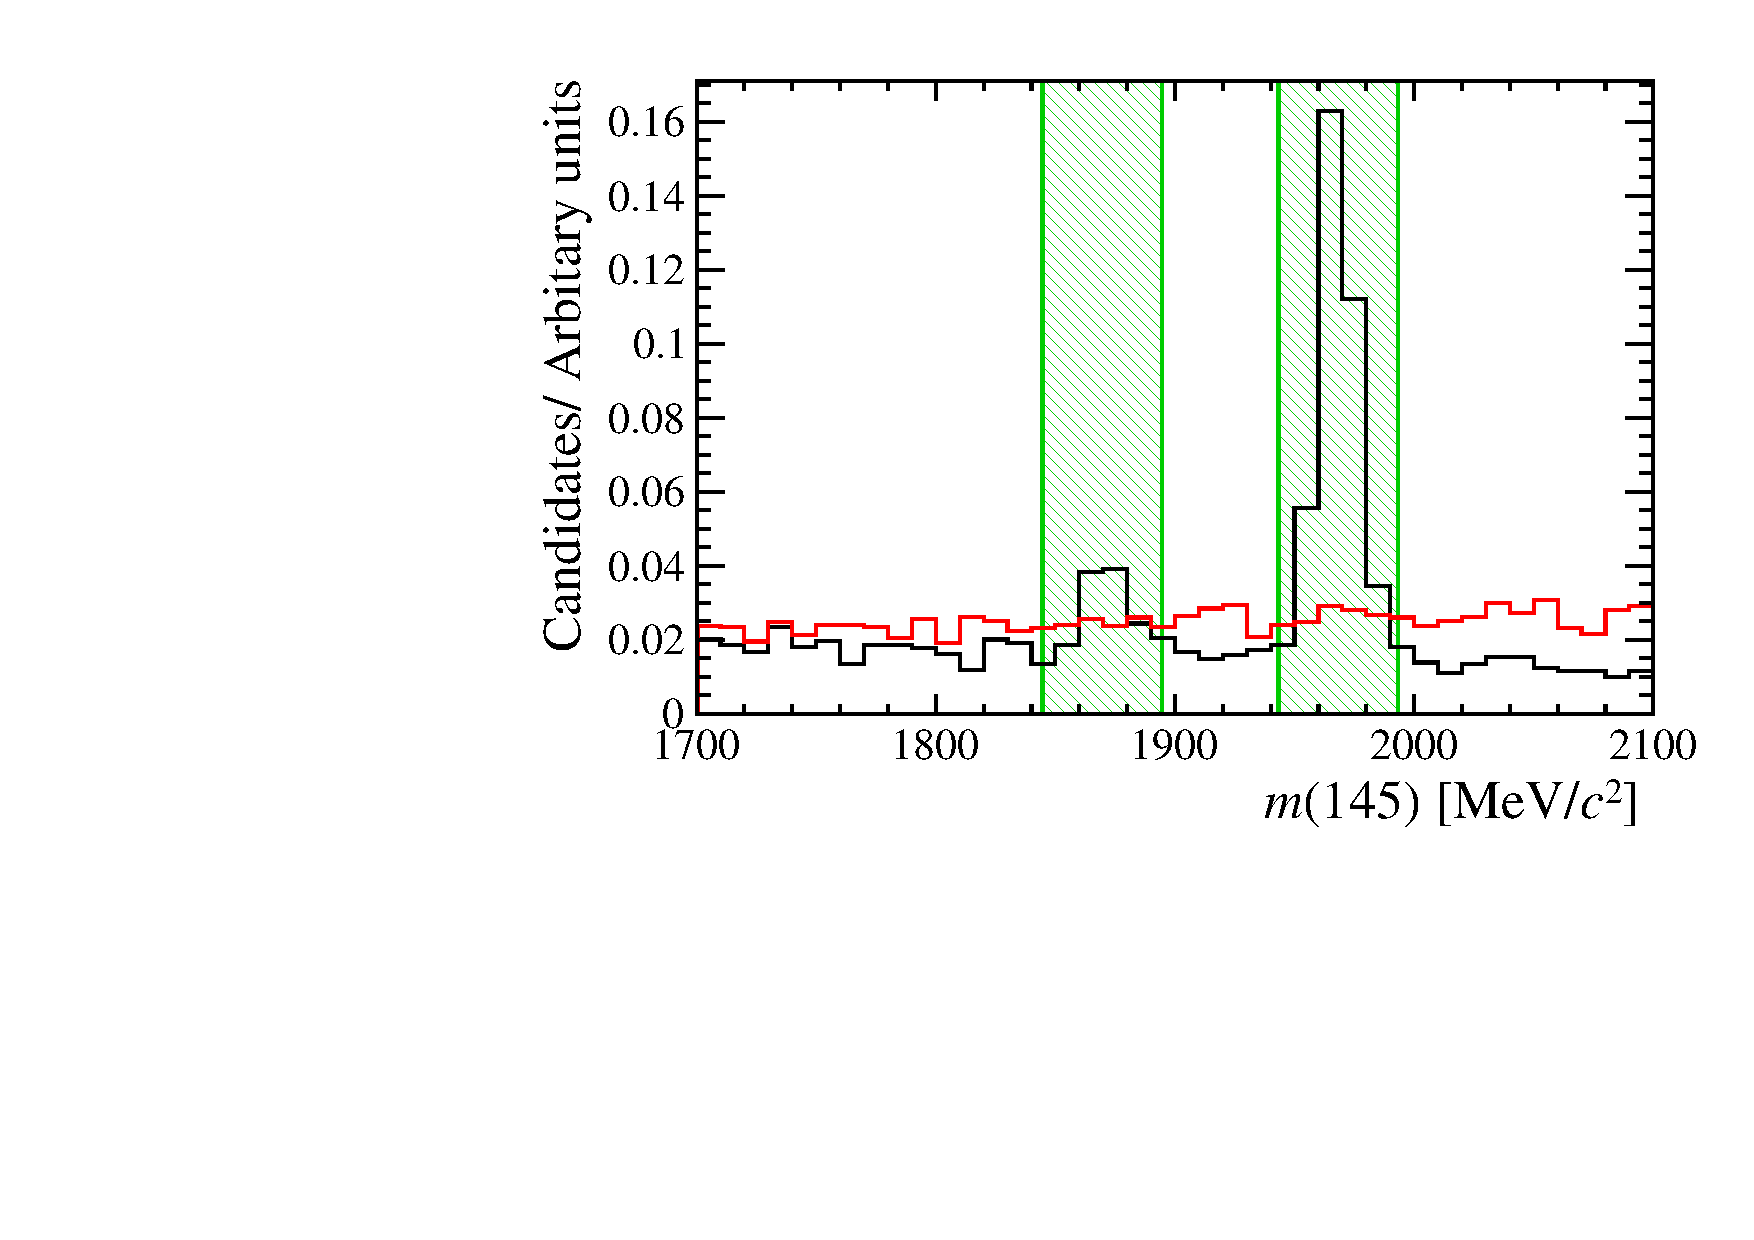
\includegraphics[width=1.0\textwidth]{figs/Selection/Veto_Comparison_B2DsPhi_Ds2PiPiPi_m145.pdf}
      \end{subfigure}
      \begin{subfigure}[t]{0.32\textwidth}
         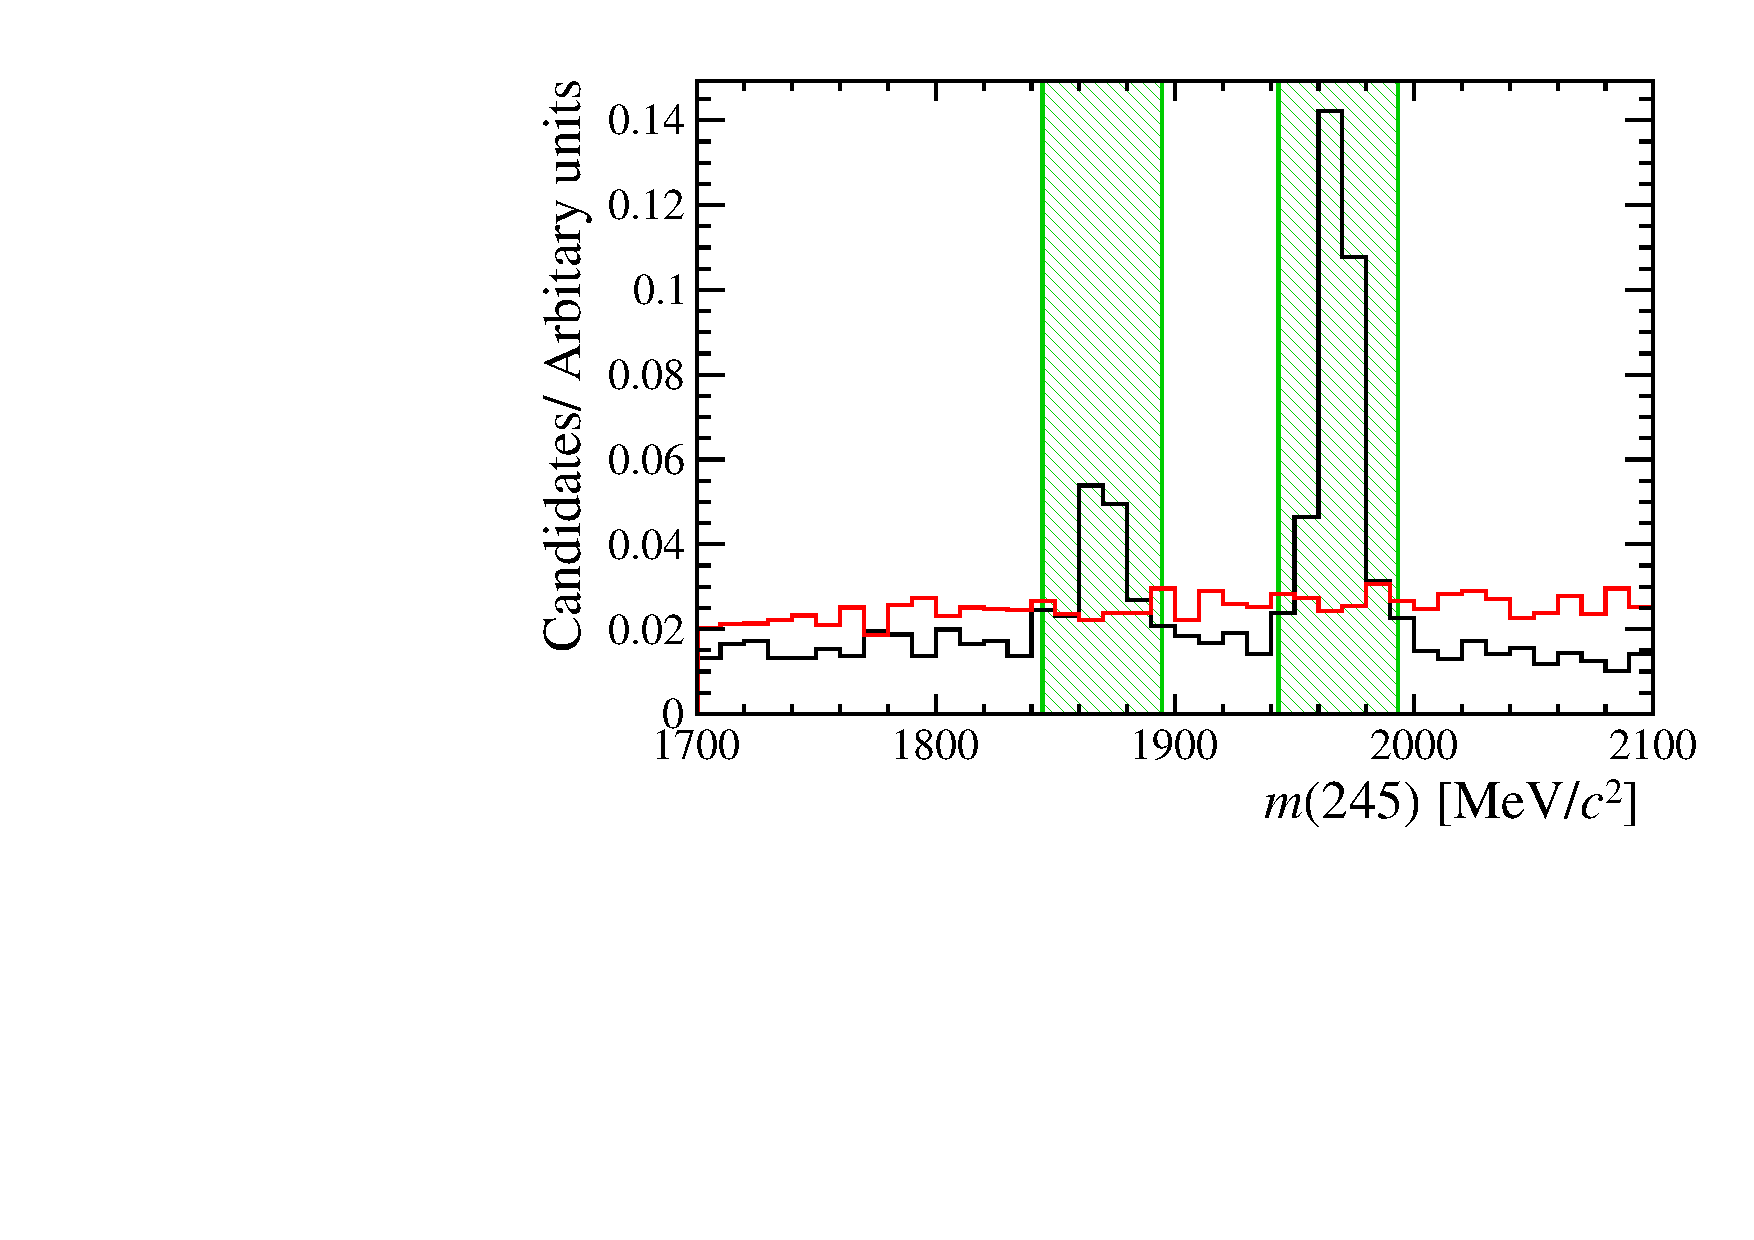
\includegraphics[width=1.0\textwidth]{figs/Selection/Veto_Comparison_B2DsPhi_Ds2PiPiPi_m245.pdf}
      \end{subfigure}
      \begin{subfigure}[t]{0.32\textwidth}
         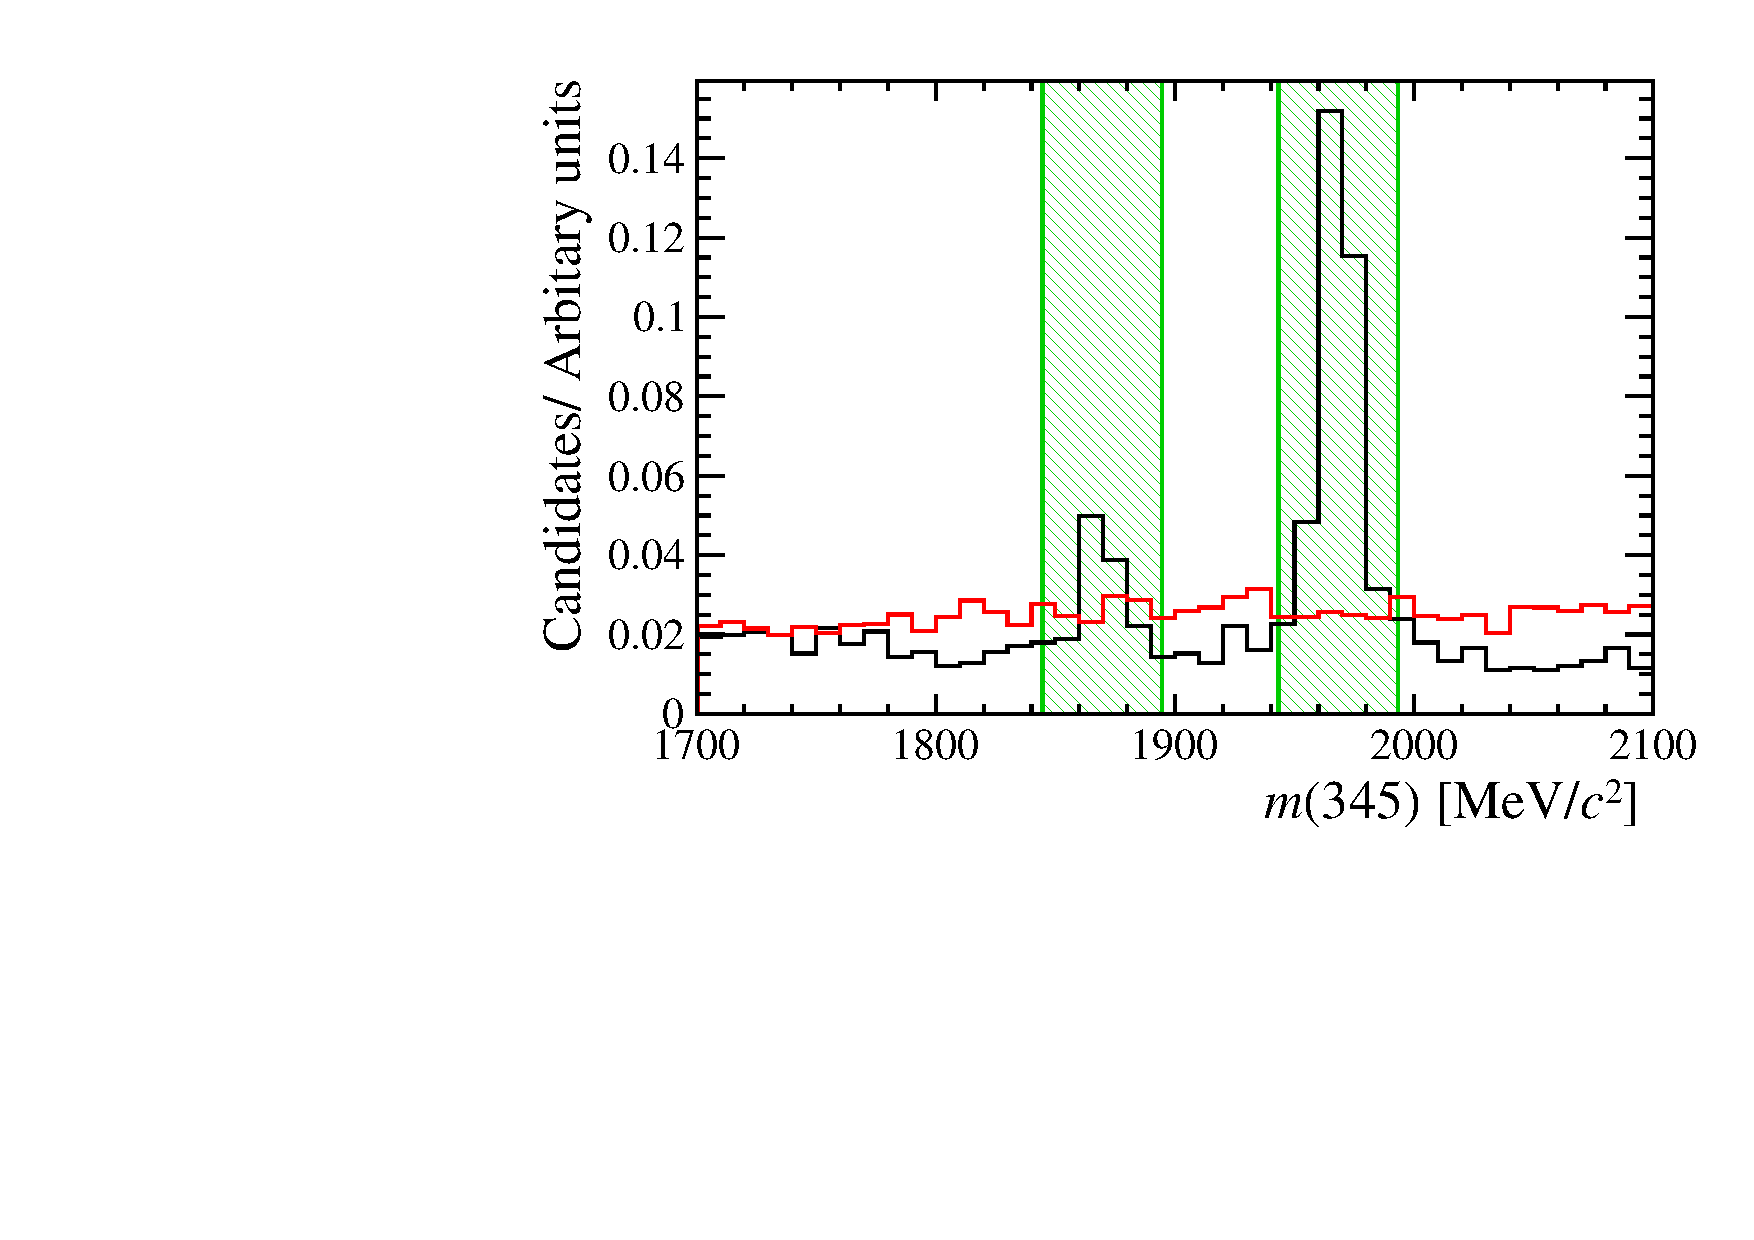
\includegraphics[width=1.0\textwidth]{figs/Selection/Veto_Comparison_B2DsPhi_Ds2PiPiPi_m345.pdf}
      \end{subfigure}
      \caption{\decay{\Bp}{(\decay{\Dsp}{\pip\pim\pip})\phiz}}
   \end{subfigure}
   \begin{subfigure}[t]{1.0\textwidth}
      \centering
      \begin{subfigure}[t]{0.32\textwidth}
         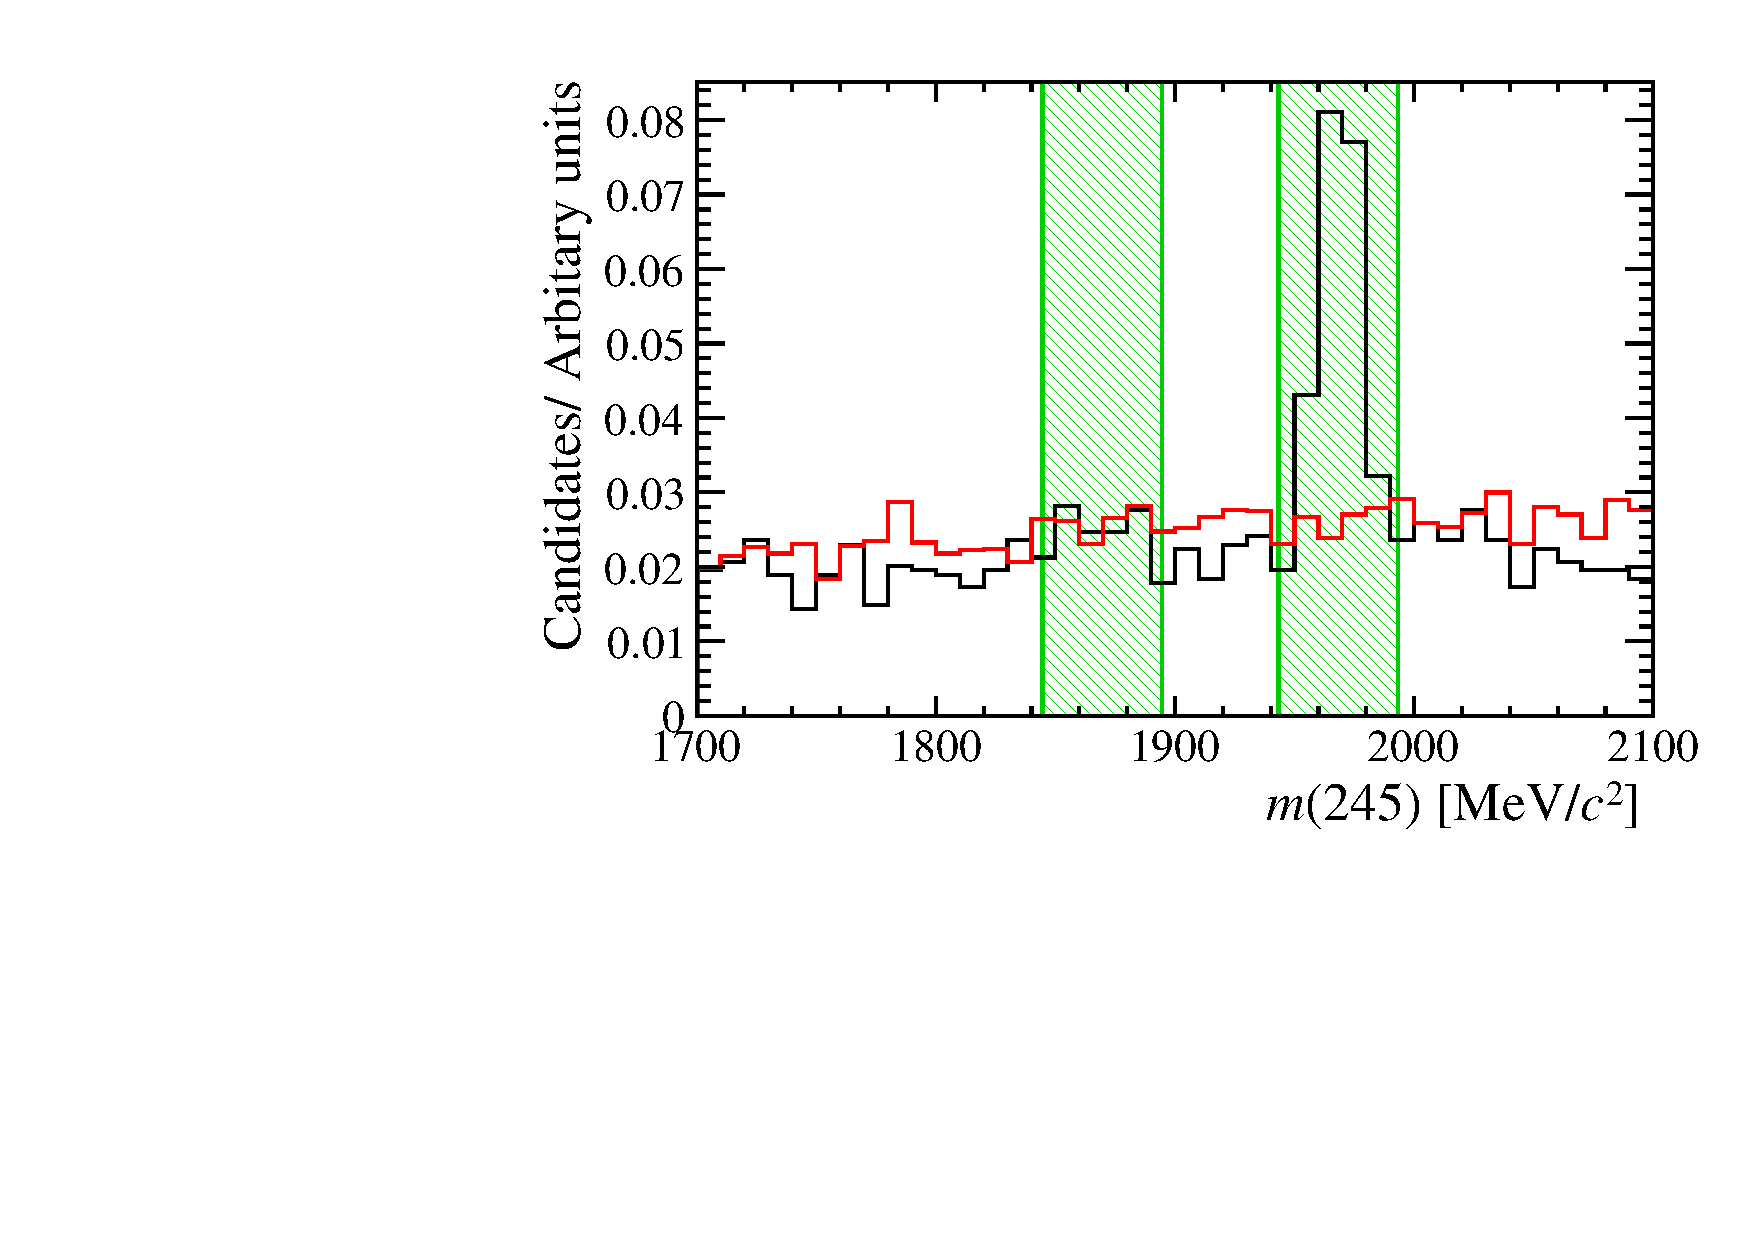
\includegraphics[width=1.0\textwidth]{figs/Selection/Veto_Comparison_B2DsPhi_Ds2KPiPi_m245.pdf}
      \end{subfigure}
      \begin{subfigure}[t]{0.32\textwidth}
         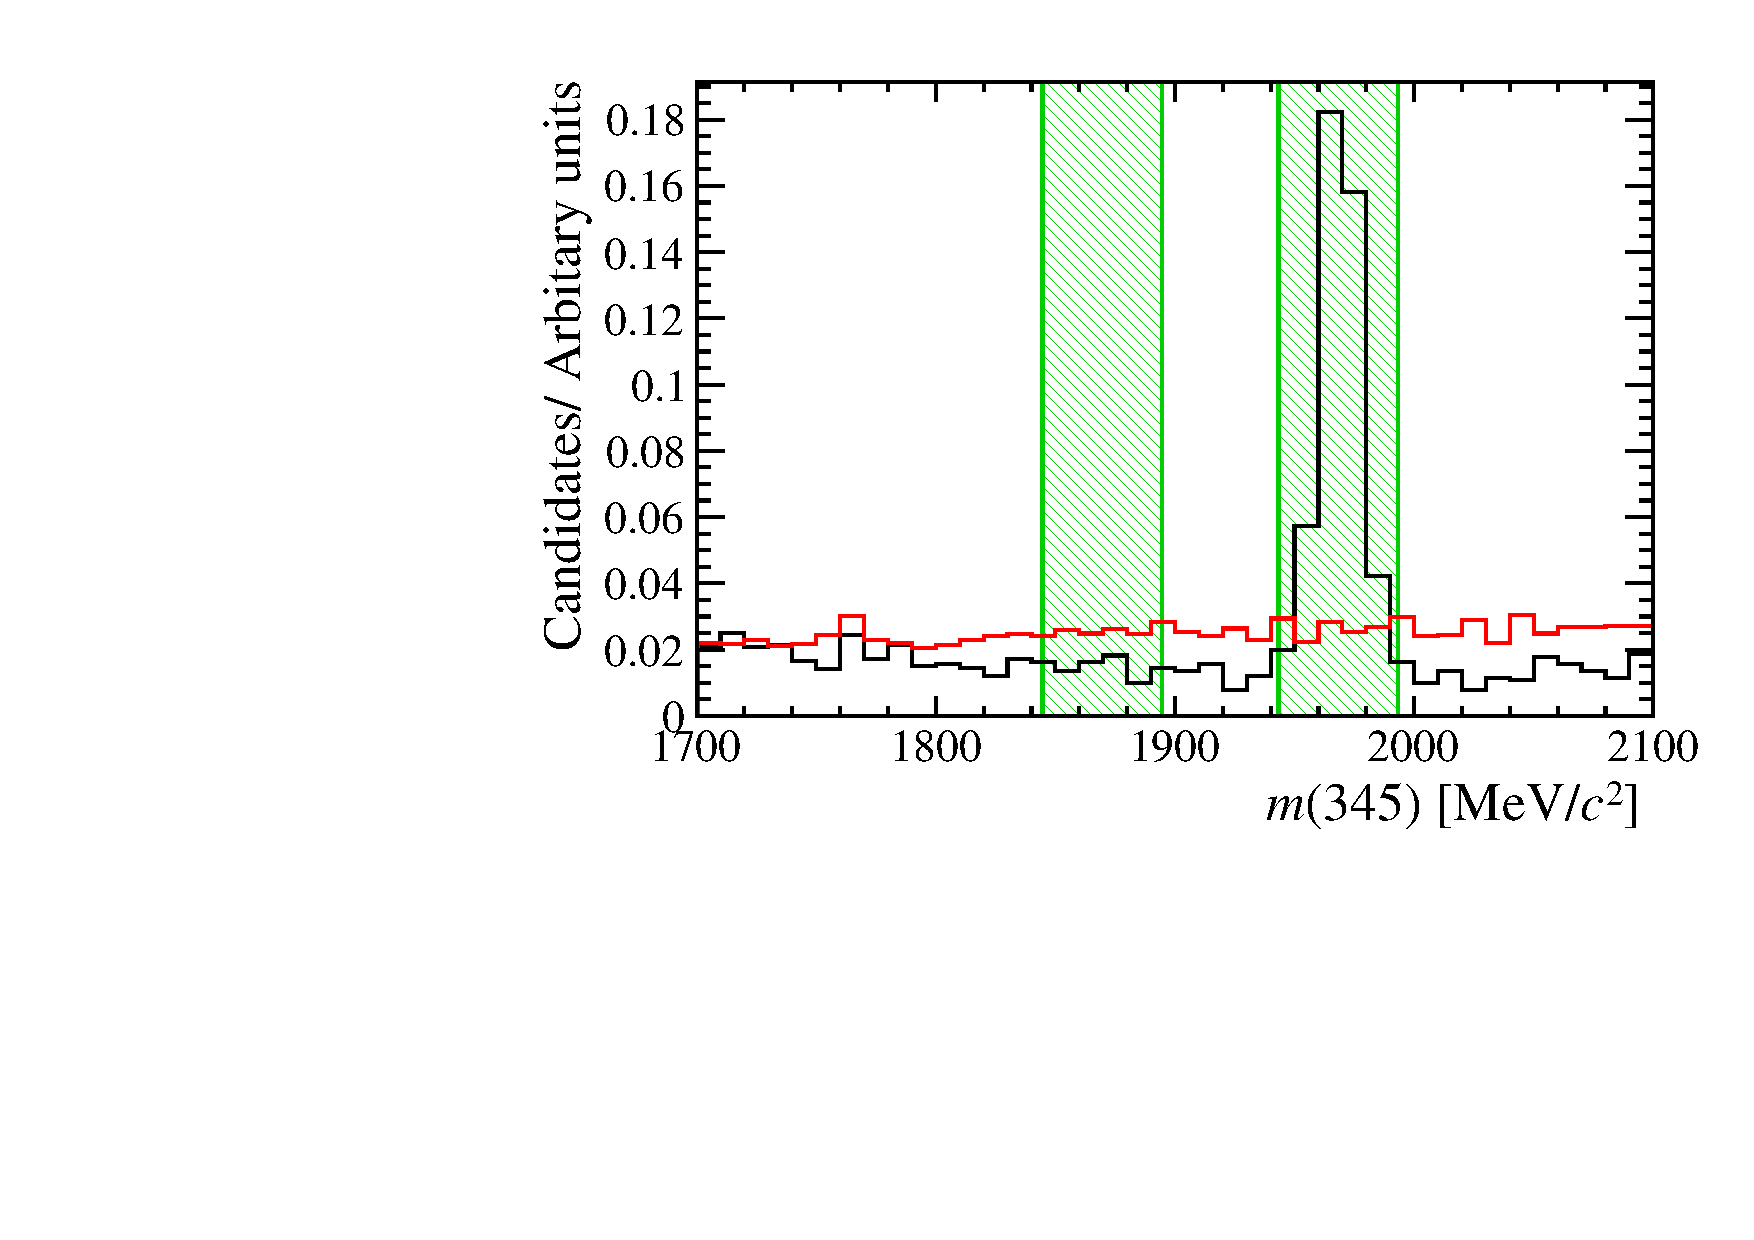
\includegraphics[width=1.0\textwidth]{figs/Selection/Veto_Comparison_B2DsPhi_Ds2KPiPi_m345.pdf}
      \end{subfigure}
      \caption{\decay{\Bp}{(\decay{\Dsp}{\Kp\pim\pip})\phiz}}
   \end{subfigure}

   \caption{Invariant mass distributions for subsets of decay products in data (black) and simulation (red). The green region show the regions removed by the vetoes listed in Sec~\ref{sec:kinematicvetos}.}
   \label{fig:invariantmassvetoes}   
\end{figure}
%%%%%%%%%%%%%%%%%%%%%%%%%%%%%%%%%%%%%%%%%%%%%%%%%%%%%%%%%%


In the search for \decay{\Bp}{\Dsp\Kp\Km} decays the increased size of the $m(\Kp\Km)$ phase-space means more of the combinations of final state particles are susceptible to sharp peaking structure from incorrectly reconstructed backgrounds. Those spectra found to have significant peaking structures are additionally vetoed, as shown in Fig.~\ref{fig:invariantmassvetoes_DsKK}.

\begin{itemize}
\item Vetoes for the mode \decay{\Bp}{(\decay{\Dsp}{\Kp\Km\pip})\Kp\Km}:
\begin{itemize}
\item $|m(\text{1245})- m(\Bs)| > 50\mevcc$
\item $|m(\text{345})- m(\Dsp)| > 25\mevcc$ and $|m(\text{345})- m(\Dp)| > 25\mevcc$
\item $|m(\text{135})- m(\Dsp)| > 25\mevcc$
\item $|m(\text{234})- m(\Dsp)| > 25\mevcc$
\end{itemize}
\end{itemize}

%%%%%%%%%%%%%%%%%%%%%%%%%%%%%%%%%%%%%%%%%%%%%%%%%%%%%%%%%%
\begin{figure}[!h]
   \centering
   \begin{subfigure}[t]{1.0\textwidth}
      \centering
      \begin{subfigure}[t]{0.32\textwidth}
         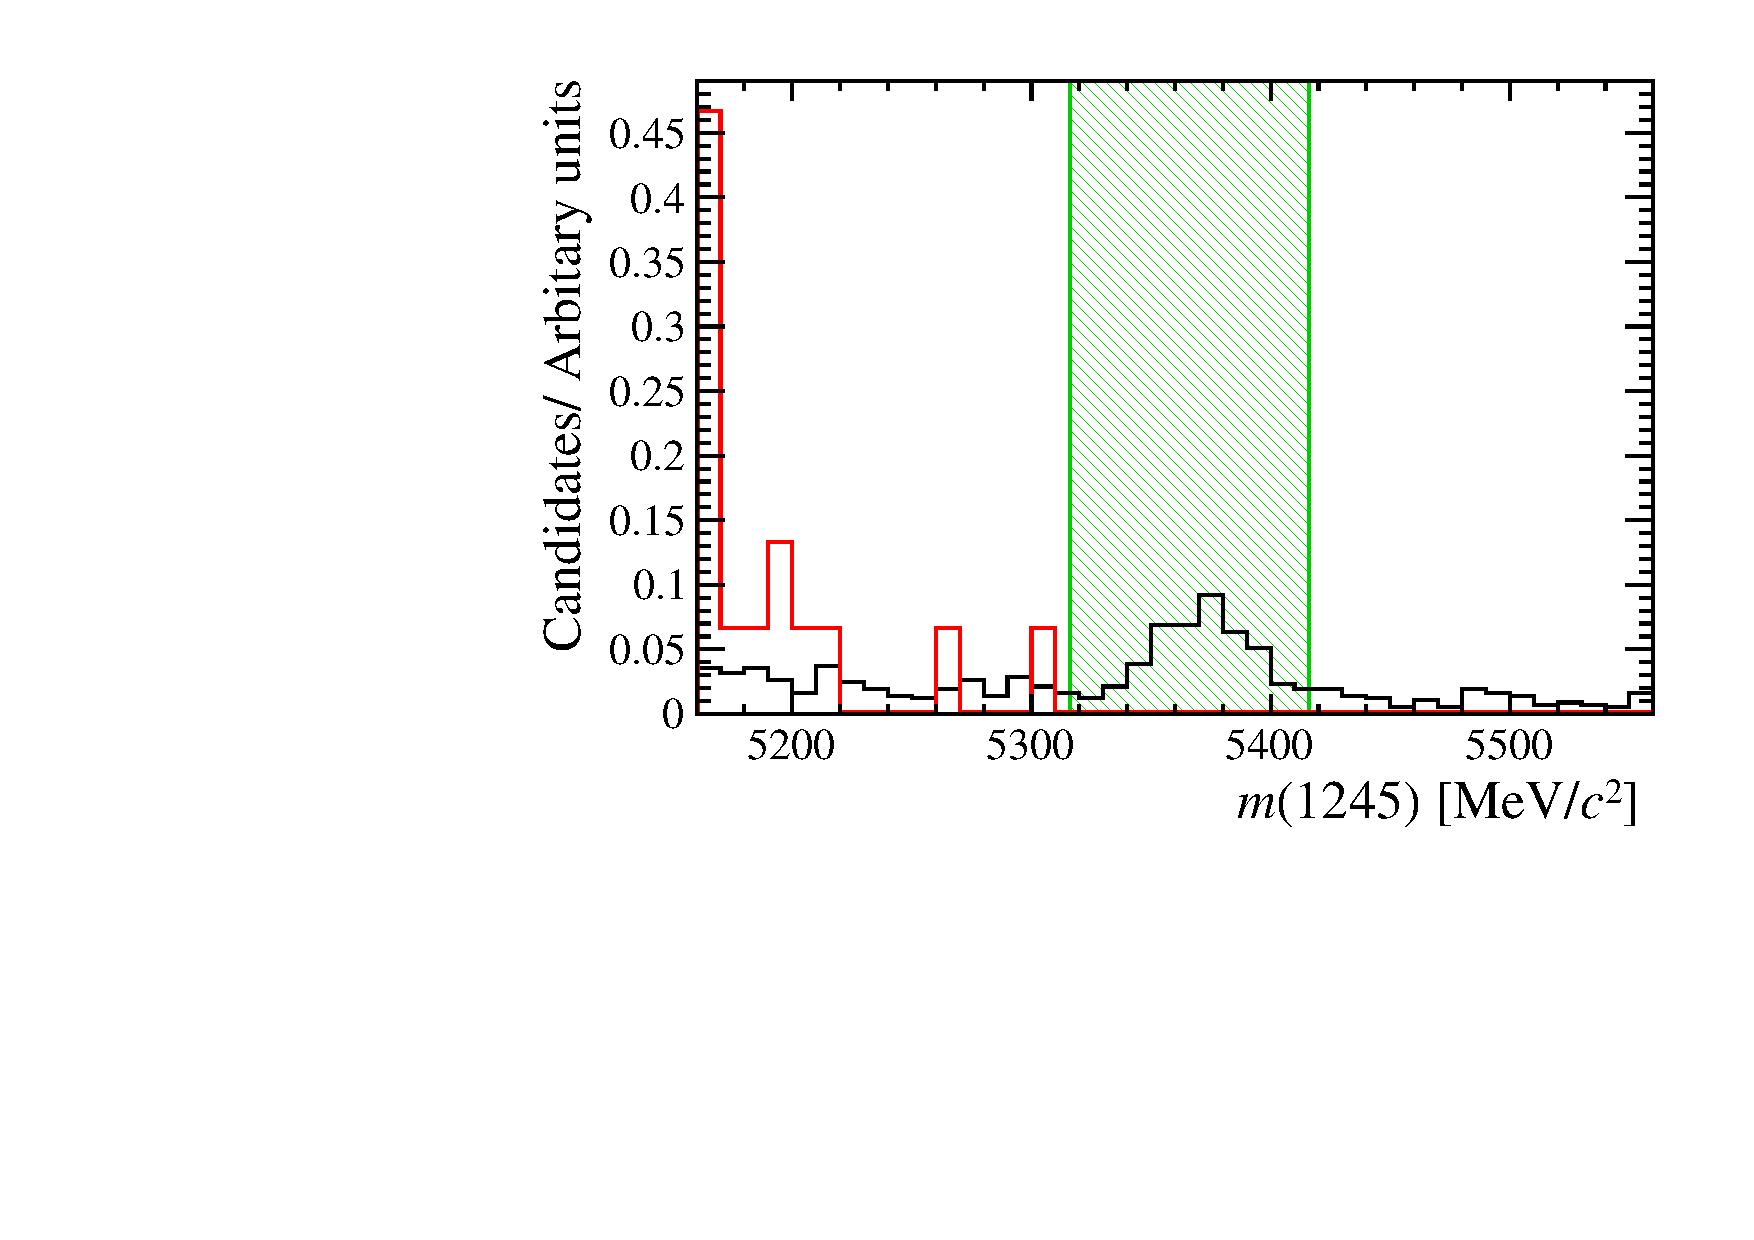
\includegraphics[width=1.0\textwidth]{figs/Selection/Veto_Comparison_B2DsKK_Ds2KKPi_m1245.pdf}
      \end{subfigure}\\
      \begin{subfigure}[t]{0.32\textwidth}
         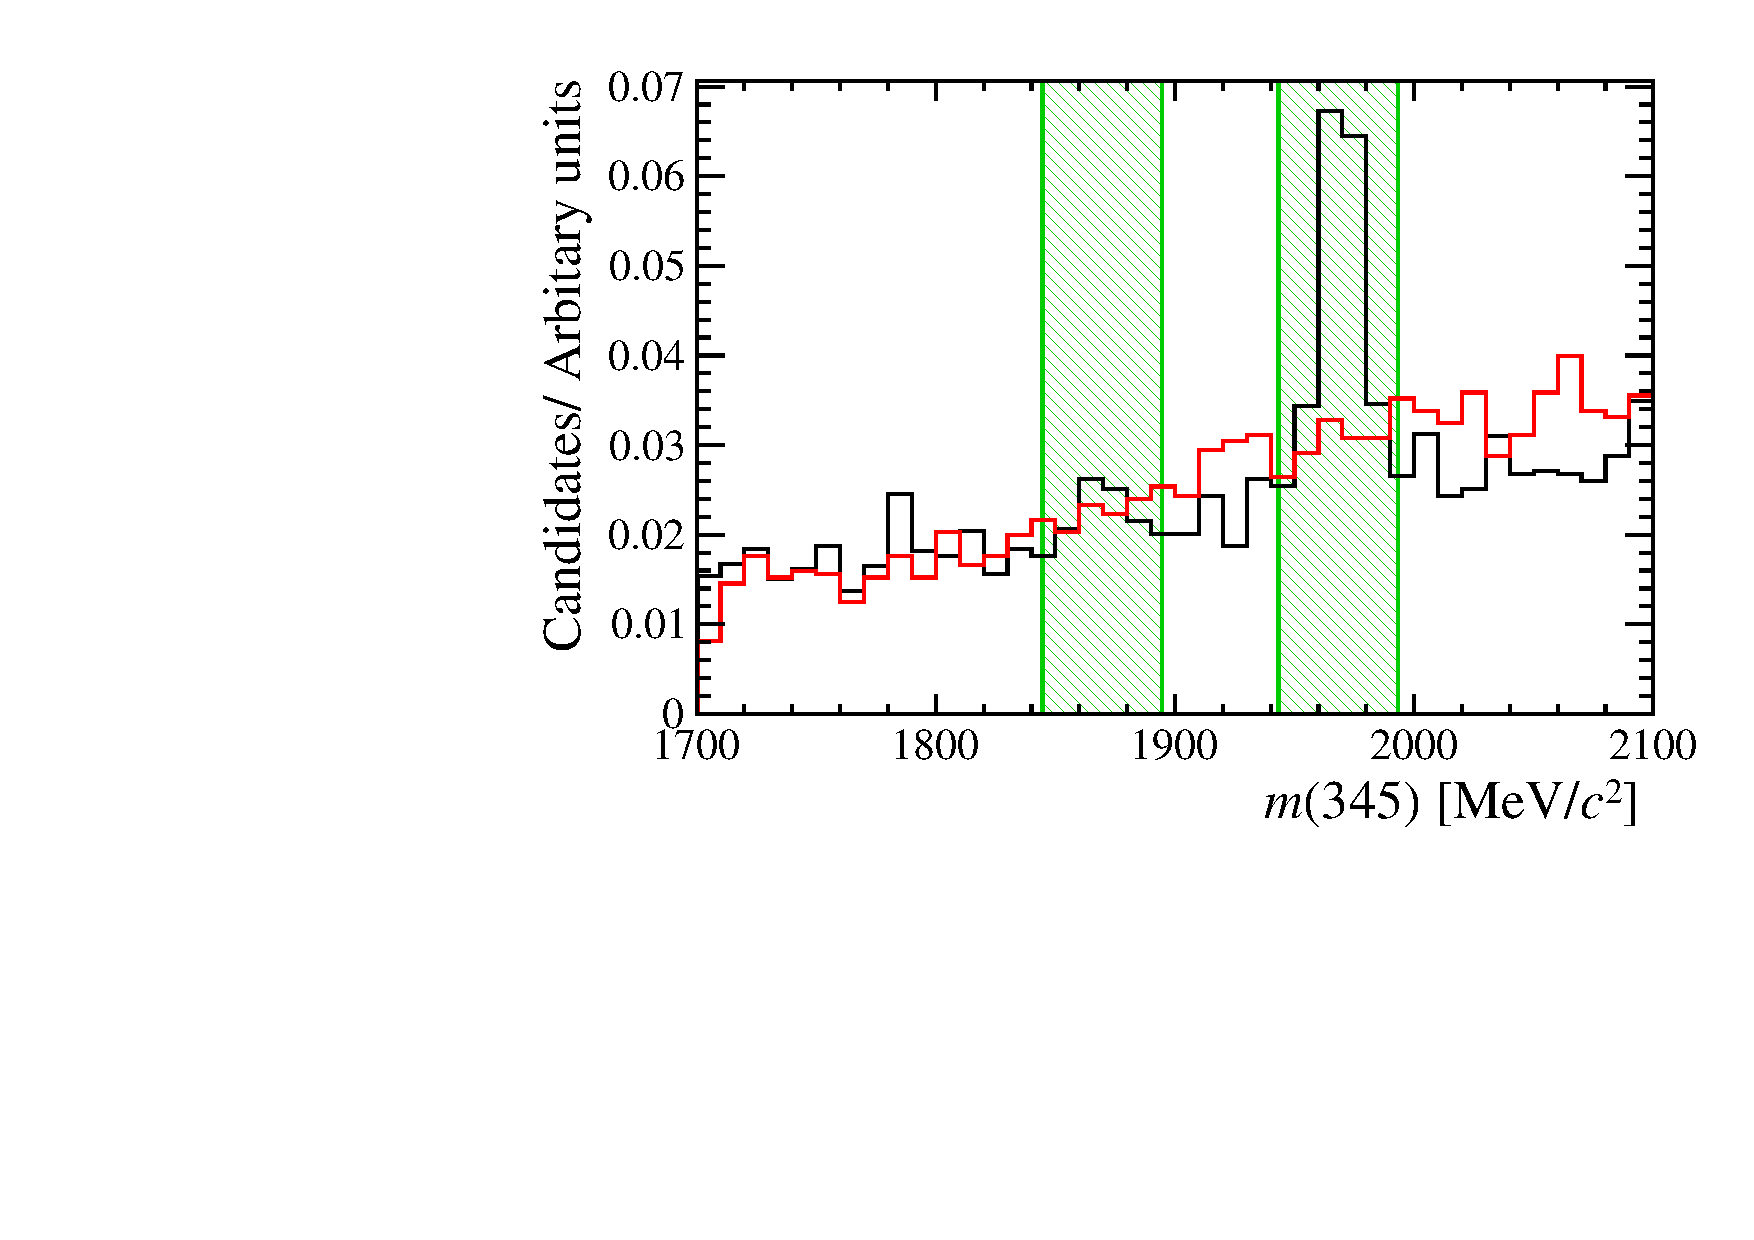
\includegraphics[width=1.0\textwidth]{figs/Selection/Veto_Comparison_B2DsKK_Ds2KKPi_m345.pdf}
      \end{subfigure}
      \begin{subfigure}[t]{0.32\textwidth}
         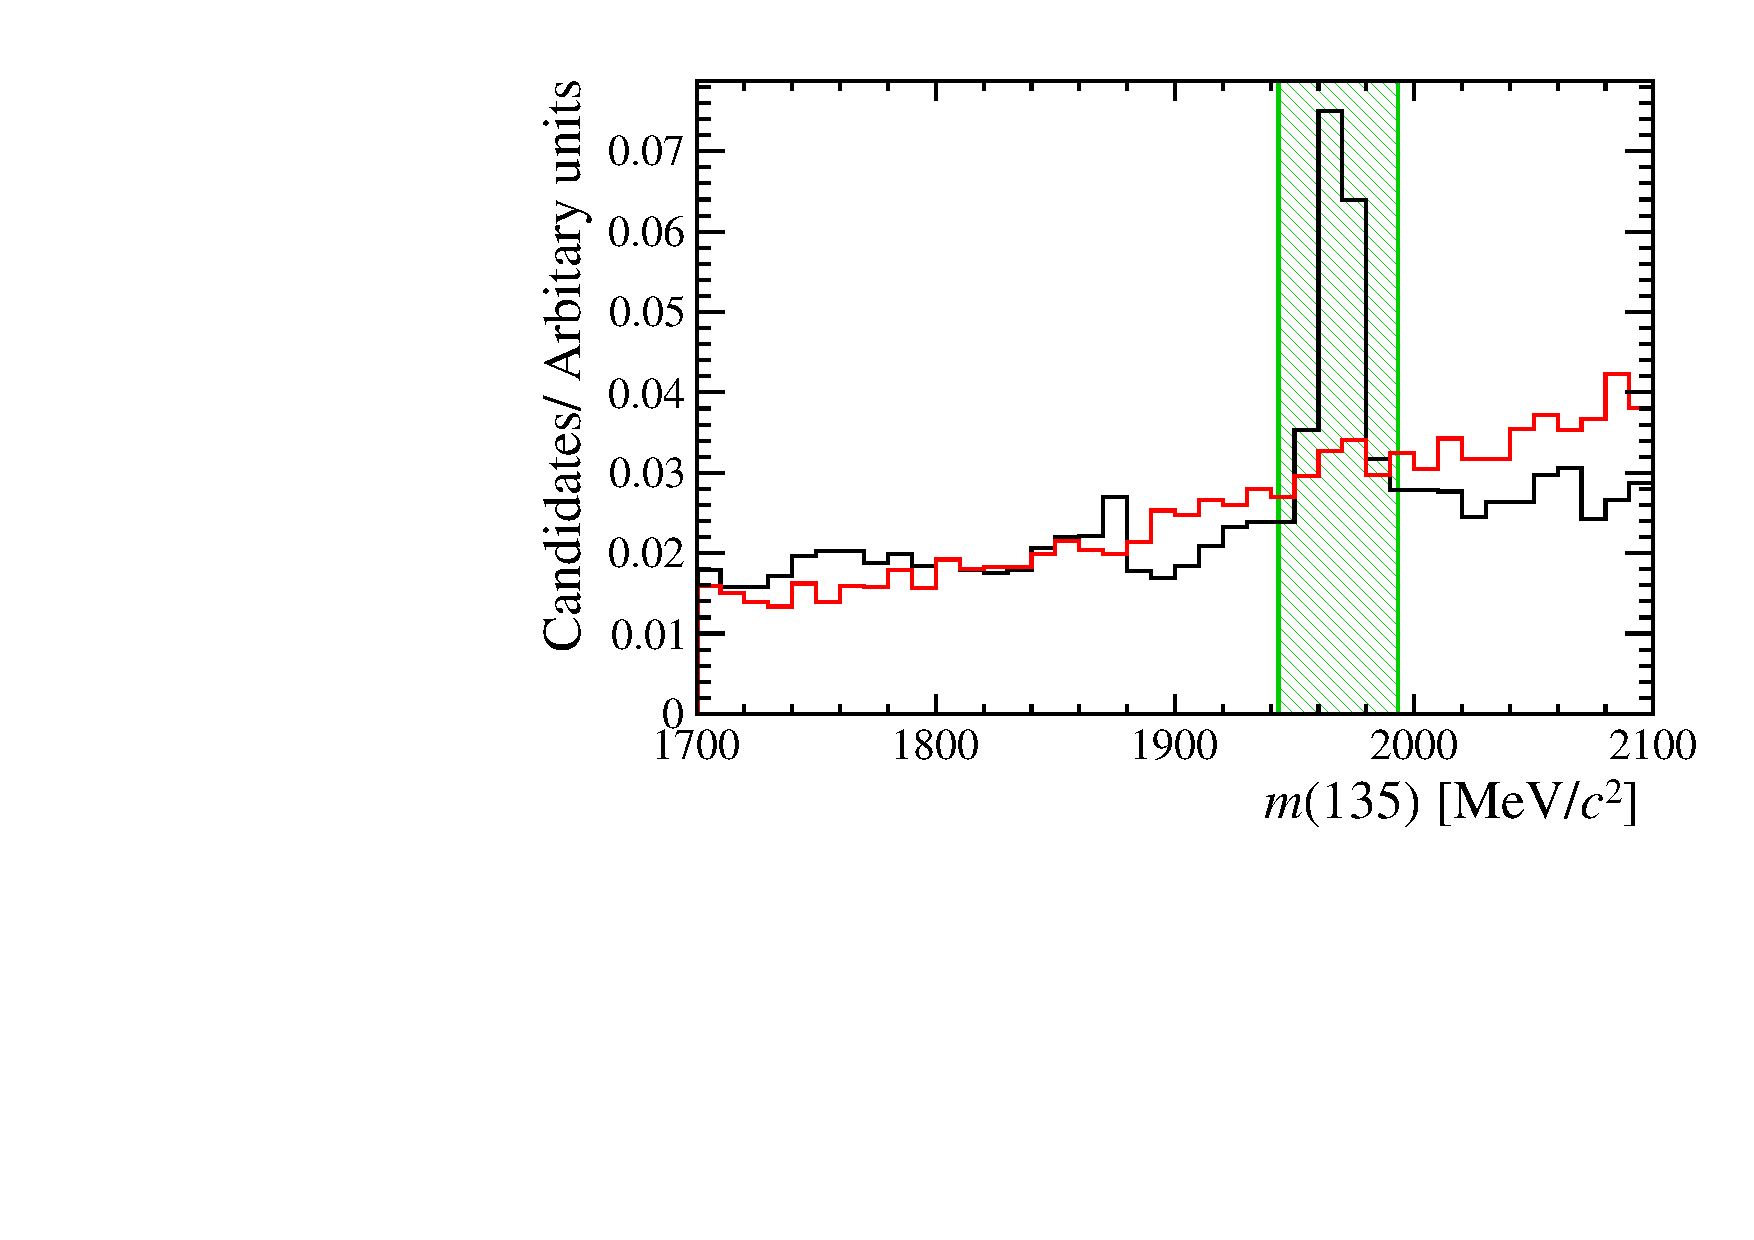
\includegraphics[width=1.0\textwidth]{figs/Selection/Veto_Comparison_B2DsKK_Ds2KKPi_m135.pdf}
      \end{subfigure}
      \begin{subfigure}[t]{0.32\textwidth}
         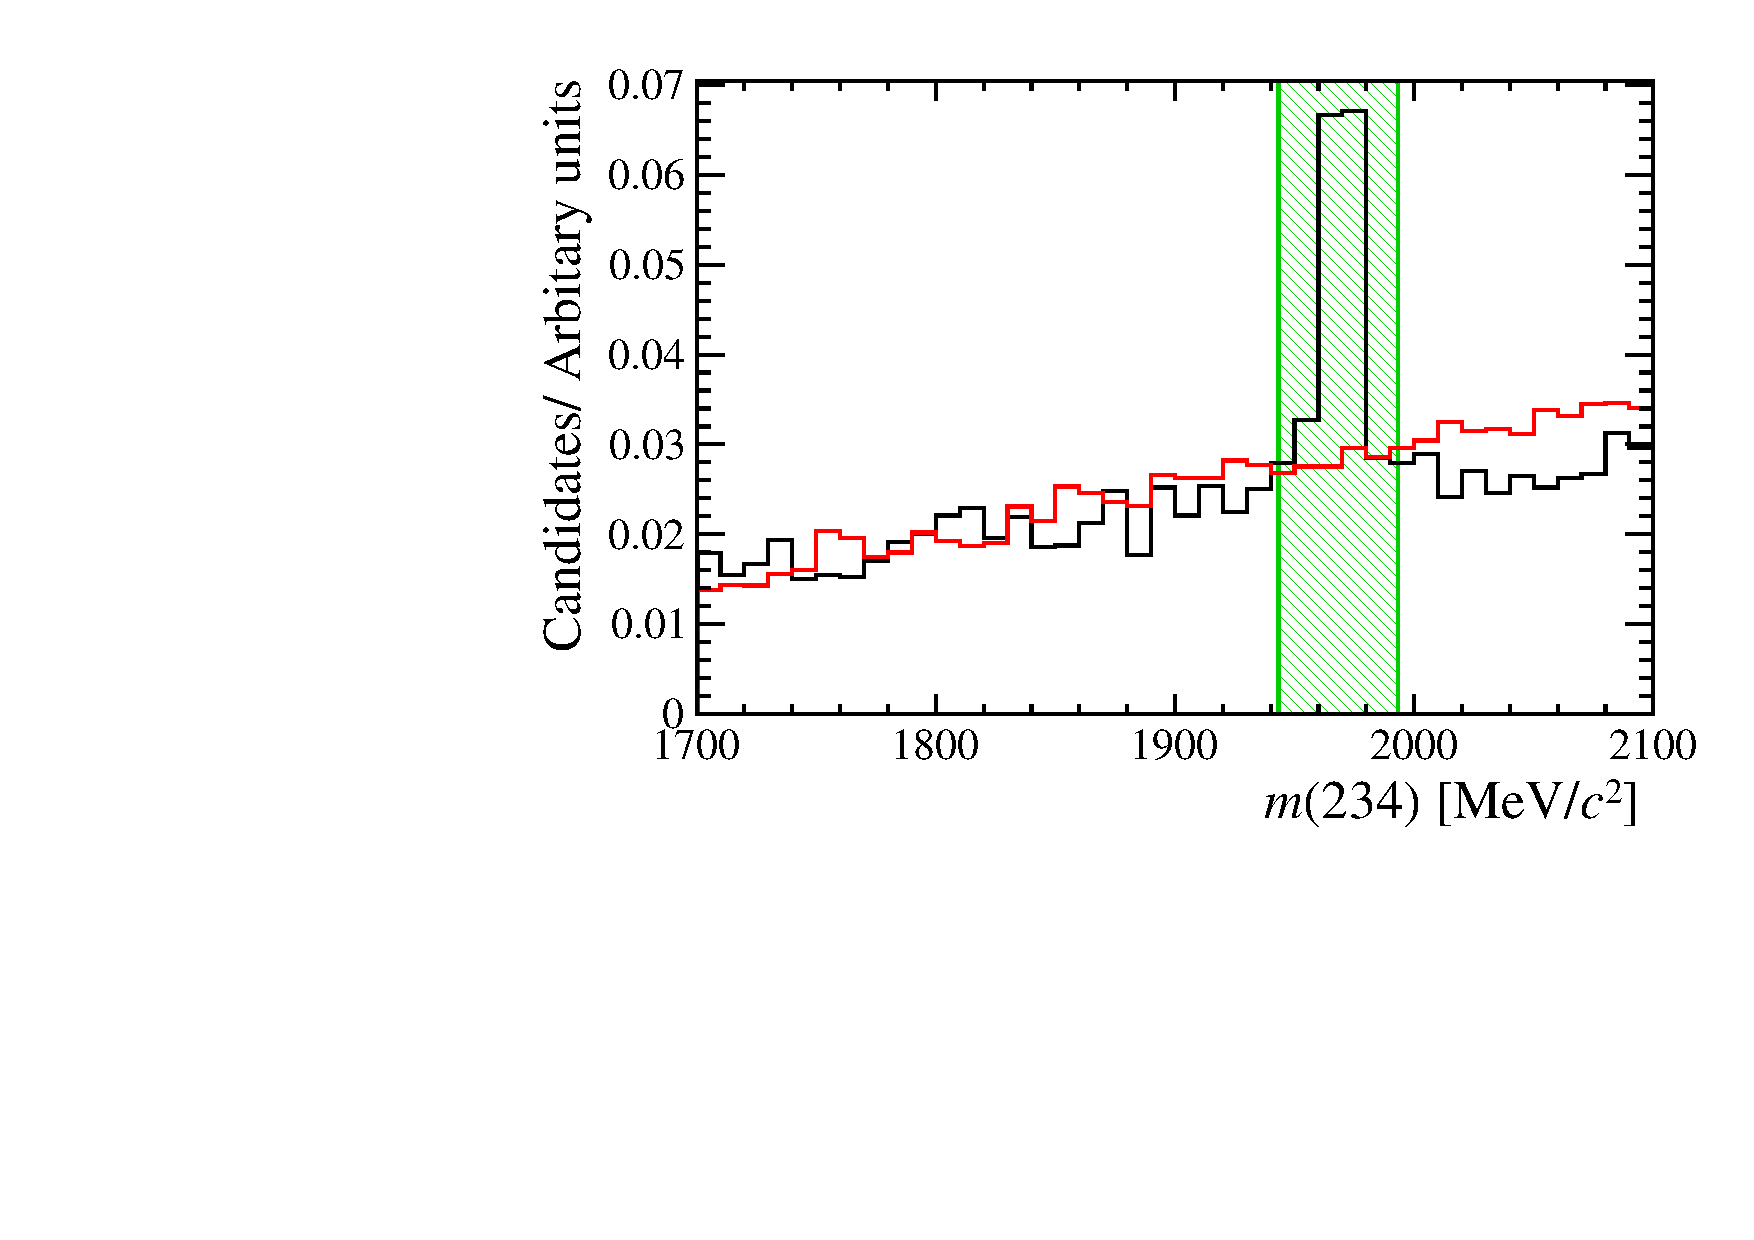
\includegraphics[width=1.0\textwidth]{figs/Selection/Veto_Comparison_B2DsKK_Ds2KKPi_m234.pdf}
      \end{subfigure}
   \end{subfigure}

   \caption{Invariant mass distributions for subsets of decay products for \decay{\Bp}{(\decay{\Dsp}{\Kp\Km\pip})\Kp\Km} decays in data (black) and simulation (red). The green region show the regions removed by the vetoes listed in Sec~\ref{sec:kinematicvetos}.}
   \label{fig:invariantmassvetoes_DsKK}   
\end{figure}
%%%%%%%%%%%%%%%%%%%%%%%%%%%%%%%%%%%%%%%%%%%%%%%%%%%%%%%%%%
 
Another set of vetoes rejects decays where the tracks forming the \Dsp candidate originate from an excited charged charm meson decay, for example $\decay{\Dstarp}{(\decay{\Dz}{h^{+}h'^{-}}) \pip}$. By requiring $\Delta m = m(h^{+}h'^{-}\pip)-m(h^{+}h'^{-}) > 150 \mevcc$ decays of this type are efficiently removed. These are applied to both the signal and normalisation modes for all \Dsp decays. 


\subsection{Normalisation mode veto}
\label{sec:normvetos}

In the search for \decay{\Bp}{\Dsp\Kp\Km} decays, the entire $m(\Kp\Km)$ phasespace is used. This ranges from the \Kp\Km mass threshold at around $990\mevcc$ to the kinematic limit at $m(\Bp) - m(\Dsp) = 3300\mevcc$. This range is wide enough to include the mass of the \Dzb meson, $m(\Dz) = 1864 \mevcc$. Consequently, when inspecting the $m(\Kp\Km)$ spectrum for selected signal candidates there is an excess of events at the \Dz mass. It is necessary to remove these from the signal samples as, unsurprisingly, they result in a peak at the \Bp mass in the $m(\Dsp\Kp\Km)$ spectrum and lead to an incorrect signal yield. As described in Section~\ref{sec:selectionrequirements}, these removed events are used as the normalisation channel for the measurement of \decay{\Bp}{\Dsp\Kp\Km} decays. 
The region affected by the veto $|m(\Kp\Km) - m(\Dzb)| > 25 \mevcc$ is shown in Fig.~\ref{fig:normalisationveto_KK}.

%%%%%%%%%%%%%%%%%%%%%%%%%%%%%%%%%%%%%%%%%%%%%%%%%%%%%%%%%%
\begin{figure}[!h]
   \centering
   \begin{subfigure}[t]{0.49\textwidth}
      \centering
      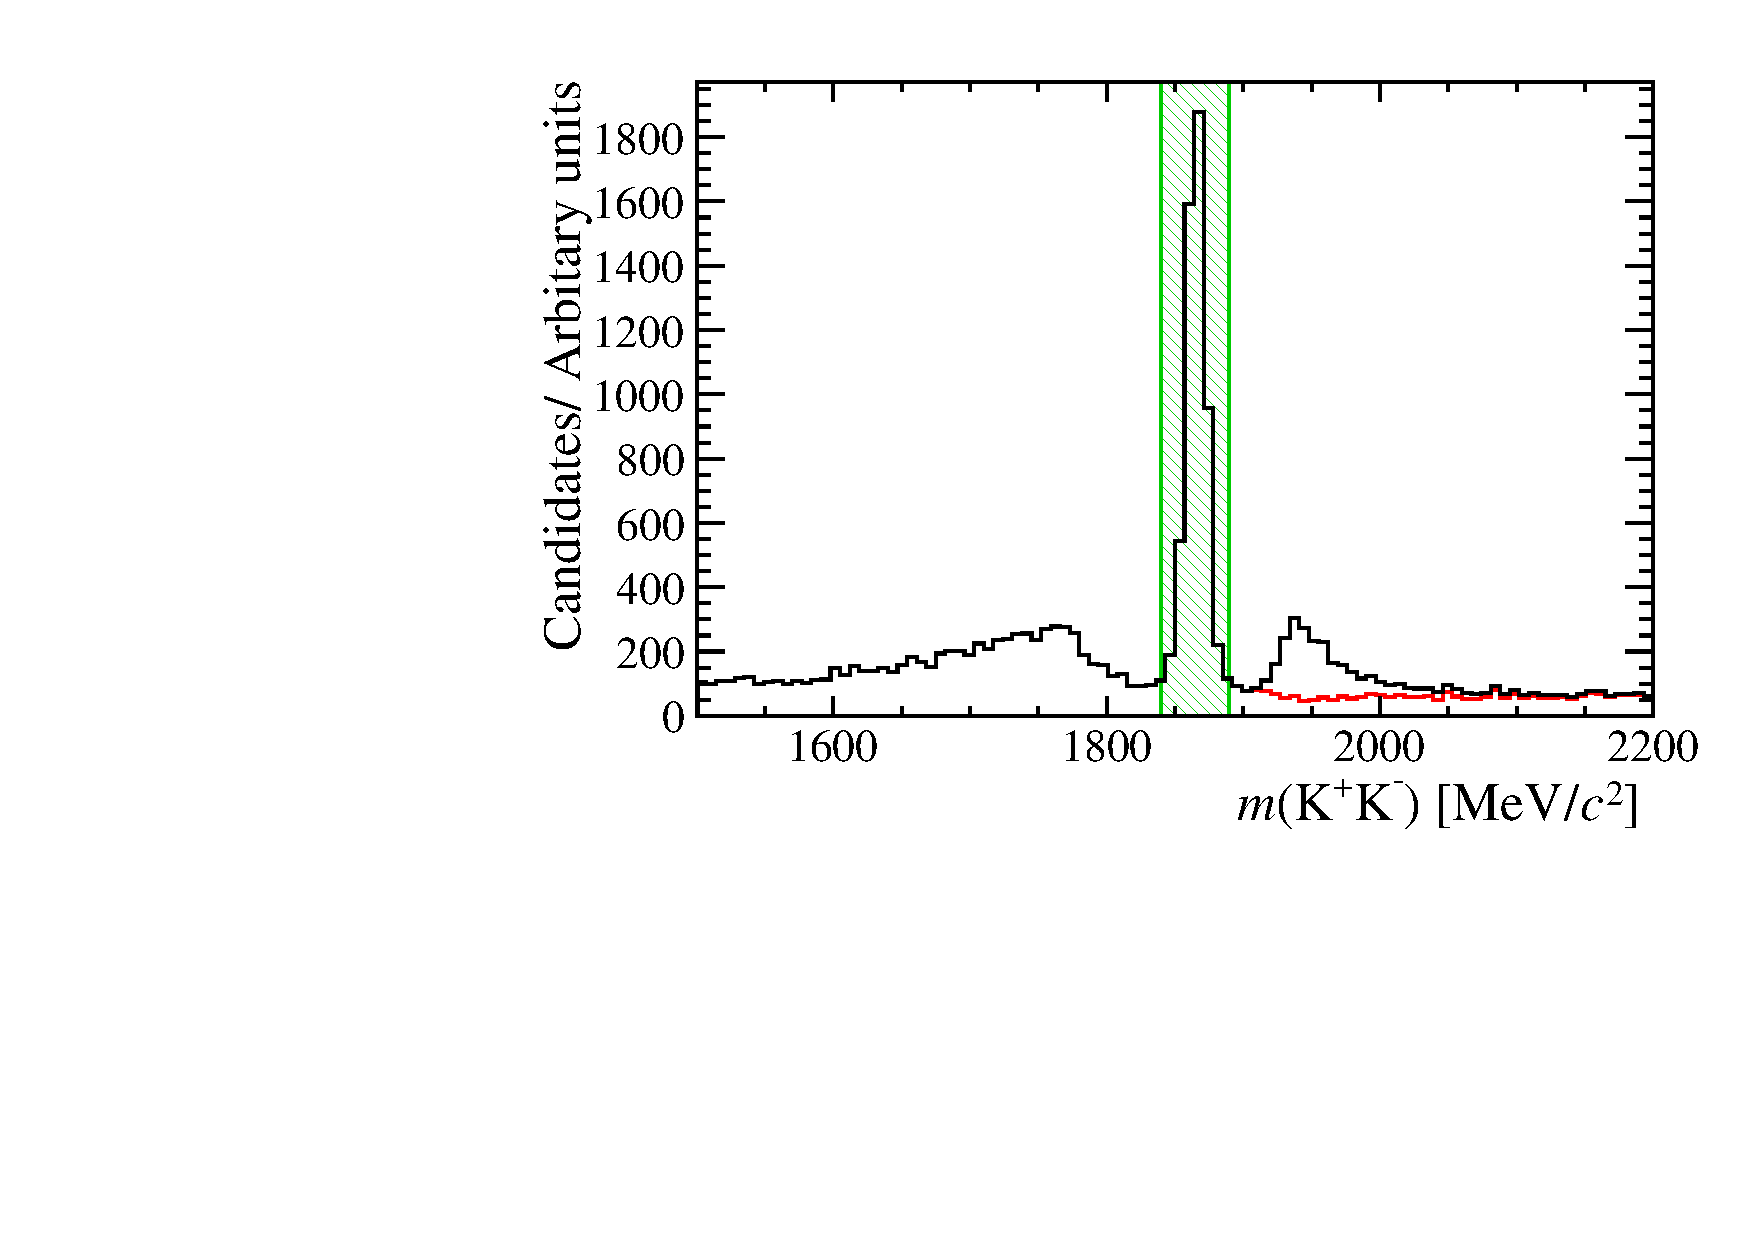
\includegraphics[width=1.0\textwidth]{figs/Selection/D0Veto_Comparison_B2DsKK_Ds2KKPi_Phi_M.pdf}
      \caption{\decay{\Dzb}{\Kp\Km} }
      \label{fig:normalisationveto_KK}
   \end{subfigure}
   \begin{subfigure}[t]{0.49\textwidth}
      \centering
      \includegraphics[width=1.0\textwidth]{figs/Selection/D0Veto_Comparison_B2DsKK_Ds2KKPi_Phi_KPi_M.pdf}
      \caption{\decay{\Dzb}{\Kp\pim} }
      \label{fig:normalisationveto_KPi}
   \end{subfigure}
   \caption{The vetoes applied to remove the normalisation channel \decay{\Bp}{\Dsp\Dzb} from the sample of \decay{\Bp}{\Dsp\Kp\Km} decays. Both the correctly reconstructed \decay{\Dzb}{\Kp\Km} (left) and mis-reconstructed \decay{\Dzb}{\Kp\pim} decays (right) are targeted. The effect of the mis-reconstructed \decay{\Dzb}{\Kp\pim} decay veto on the $m(\Kp\Km)$ distribution is shown in red in the left plot.}
   \label{fig:normalisationveto}   
\end{figure}
%%%%%%%%%%%%%%%%%%%%%%%%%%%%%%%%%%%%%%%%%%%%%%%%%%%%%%%%%%


In addition to the correctly reconstructed normalisation channel, the presence of the incorrectly reconstructed \decay{\Bp}{\Dsp(\decay{\Dzb}{\Kp\pim})} decay is observable in Fig.~\ref{fig:normalisationveto_KK}. This appears as smeared out peak to the right of the \Dzb peak. Although the probability of the \pim meson being misidentified as a \Km meson is low, the branching fraction for \decay{\Dzb}{\Kp\pim} is larger, leading to the observed excess. It is possible, and necessary, to remove this contribution. The \Kp\Km candidates are reconstructed again, swapping the mass hypothesis of the second track from \Km to \pim. The distribution of these candidates in the vicinity of the \Dzb mass is shown in Fig.~\ref{fig:normalisationveto_KPi}. A distinct peak is observed at the \Dzb mass. This contribution is removed by the requirement $|m(\Kp\pim) - m(\Dzb)| > 25 \mevcc$. The effect of this requirement on the $m(\Kp\Km)$ spectrum is shown by the red line in Fig.~\ref{fig:normalisationveto_KK}, which represents the sample with this veto applied. The \decay{\Bp}{\Dsp(\decay{\Dzb}{\Kp\pim})} background is reduced to a negligible level.

Another structure appears to be present to the left of the \Dzb peak in Fig.~\ref{fig:normalisationveto_KK}. This is likely to be due to \decay{\Dzb}{\Kp\Km X} decays in which one or more particles have not been reconstructed. This partially reconstructed background would not peak at the \Bp mass in the $m(\Dsp\Kp\Km)$ spectrum due to the missing particles, therefore no attempt is made to remove this contribution.


\subsection{Multivariate analysis}

Multivariate Analyses (MVAs) are used to help discriminate between genuine \Dsp and \phiz meson decays and combinations of unrelated tracks. 
These MVAs are trained on data using large samples of \B mesons decays which have similar topologies. 
This data-driven approach can benefit from an expanded set of variables that are not perfectly represented in simulation, including track quality and particle identification information, in addition to the widely used kinematic and geometric properties.
The method is based on the approach used in Ref.~\cite{LHCb-PAPER-2012-050}, however the choice of input variables has been optimised and training samples expanded to include Run II data.

The sample of \Dsp mesons is obtained from the relatively abundant \decay{\Bsb}{\Dsp\pim} decay. Similarly, the sample of \phiz mesons is obtained from \decay{\Bs}{\jpsi\phiz} decays. Large, high purity samples are reconstructed using similar requirements to those applied in the selection of signal \Dsp and \phiz mesons.
A sample is selected for each of the \Dsp and \phiz meson decays uses in this analysis, as listed in Table~\ref{tab:mva_modes}. 
The training of separate MVAs for the different \Dsp modes allows the use of particle identification variables that separate kaons and pions to be fully exploited.
The MVA trained using \decay{\Bs}{\jpsi(\decay{\phiz}{\Kp\Km})} decays is used to select both \decay{\phiz}{\Kp}{\Km} and \decay{\Dzb}{\Kp\Km} decays. For the normalisation mode this may be suboptimal, however it ensures the selection of the signal and normalisation channels are almost identical such that the systematic uncertainty in the ratio of efficiencies is minimised.
The samples of \decay{\Bsb}{\Dsp\pim} and \decay{\Bs}{\jpsi\phiz} decays are randomly split into two subsamples. The first is used to train the MVAs and the second is used to determine the efficiency of the selection. To prevent the difference between \phiz and \Dzb decays from affecting the ratio of efficiencies, the normalisation channel MVA efficiency is instead determined from a dedicated sample of \decay{\Dzb}{\Kp\Km} decays as detailed in Table.~\ref{tab:mva_modes}. The \decay{\phiz}{\Kp\Km} MVA is also used to select the \Kp\Km pair in \decay{\Bp}{\Dsp\Kp\Km} decays.
A total of eight MVAs are trained, one for each of the \Dsp and \phiz modes, in both Run I and Run II. Changes to the particle identification variables between the two running periods necessitates separate trainings. 


\begin{table}[h]
\centering
\begin{tabular}{lll}
   \hline
   Sample                    & Mode                       & Use \\ 
   \hline
   \decay{\Bsb}{\Dsp\pim}    & \decay{\Dsp}{\Kp\Km\pip}   & Training, Efficiency \\
   \decay{\Bsb}{\Dsp\pim}    & \decay{\Dsp}{\Kp\pim\pip}  & Training, Efficiency \\
   \decay{\Bsb}{\Dsp\pim}    & \decay{\Dsp}{\pip\pim\pip} & Training, Efficiency \\
   \decay{\Bs}{\jpsi\phiz}   & \decay{\phiz}{\Kp\Km}      & Training, Efficiency \\
   \hline
   \decay{\Bp}{\Dzb\pip}     & \decay{\Dzb}{\Kp\Km}       & Efficiency          \\
   \hline
\end{tabular}

\caption{The decay modes used to train and determine the efficiency of the various MVAs used in this analysis.}
\label{tab:mva_modes}
\end{table}

\subsubsection{Preselection}

Before the samples of \Dsp and \phiz mesons are used to train the MVAs, precautions are taken to ensure the samples are representative of the \decay{\Bp}{\Dsp\phiz} and \decay{\Bp}{\Dsp\Kp\Km} signal decays. The \decay{\Bsb}{\Dsp\pim} and \decay{\Bs}{\jpsi\phiz} decays are selected using a similar procedure to the signal modes. Firstly, \emph{Stripping Lines} reconstruct the candidates. The \decay{\Bsb}{\Dsp\pim} decays are built using the same software module as the signal and normalisation channel. Therefore, the selection requirements for \Dsp candidates in \decay{\Bsb}{\Dsp\pim} decays are identical to those listed for the signal in Table~\ref{tab:strippinglinecuts}.
The \decay{\Bs}{\jpsi\phiz} decays are reconstructed using \decay{\jpsi}{\mup\mun} decays, therefore they are built using a different software module as the final state is not fully hadronic. As such there are some differences in the selection requirements for the \phiz mesons from the two sources. In general the selection requirements for the \decay{\Bs}{\jpsi\phiz} channel are looser as the presence of the muons allows an efficient triggering without the need to make tight selections on the \Kp\Km pair. A direct comparison of the relevant quantities are listed in Table~\ref{tab:strippingrequirments_phi}.

% Phi_P > 7000 && 
% Phi_FDCHI2_OWNPV >15 && 
% Phi_K0_P > 2000 && 
% Phi_K1_P > 2000 && 
% Phi_K0_IPCHI2_OWNPV > 4 && 
% Phi_K1_IPCHI2_OWNPV > 4 &&
% Phi_DIRA_OWNPV>0 && 
% Phi_ENDVERTEX_CHI2<16 && 
% Phi_K0_TRACK_GhostProb<0.4&& 
% Phi_K1_TRACK_GhostProb<0.4 && 
% (Phi_K0_PT+Phi_K1_PT)>1000)

\begin{table}[h]
\centering
\begin{tabular}{ l l l l }
\hline
Particle       & Quantity                       &  Signal                              & Control                                 \\  
\hline
\phiz          & Mass minimum                   &  $870\mevcc$                         & $980\mevcc$ \\ 
               & Mass maximum                   &  $1170\mevcc$                        & $1050\mevcc$ \\ 
               & Transverse Momentum            &  -                                   & $\pt > 500 \mevc$                       \\  
               & Products \pt scalar sum        &  $\sum{|\pt|} > 1000 \mevc$          &  -                                      \\  
               & $\text{DOCA}(\Kp,\Km)$         &  $ < 0.5\mm$     &  -                                      \\  
               & Direction angle                &  $\cos{\theta}>0$                    &  -                                      \\  
               & Vertex quality                 &  $\chi^{2}/N_{\text{DOF}} < 16$      & $\chi^{2}/N_{\text{DOF}} < 25$          \\   
               & Flight distance significance   &  $\chi^{2}_{\text{FD} }  > 16$       &  -                                      \\ 
\hline
\Kpm           & Track quality                  &  $\chi^{2}/N_{\text{DOF}}<4.0$       &  $\chi^{2}/N_{\text{DOF}}<5.0$          \\  
               & Transverse momentum            &  $\pt > 100 \mevc$                   &  -                                      \\  
               & Momentum                       &  $\ptot > 1000 \mevc$                &  -                                      \\  
               & Impact parameter significance  &  $\chi^{2}_{\text{IP}} > 4$          &  -                                      \\  
               & Ghost track probability        &  $P_{\text{Ghost}} < 0.4$            &  -                                      \\
               & Particle identification        &  $\text{PIDK}>-10$                   & $\text{PIDK}>0$                         \\ 
\hline
\end{tabular}

\caption{The \emph{Stripping Line} requirements for \decay{\phiz}{\Kp\Km} candidates in the signal and MVA training (control) mode selection. All requirements are looser for the control channel with the exception of the particle identification requirements.}
\label{tab:strippingrequirments_phi}
\end{table}

The difference in the two selections could be potentially biasing when calculating the efficiency of the MVA, therefore the requirements are tightened on the half of the \decay{\Bs}{\jpsi\phiz} sample used to calculate the efficiency. The looser set of requirements are still used when training the MVA methods to maximise the sample sizes to help prevent overtraining. When training the MVAs the \phiz meson invariant mass sidebands in the \decay{\Bs}{\jpsi\phiz} sample are used as the background sample. It was found that using the tighter set of requirements led to a negligible amount of background candidates, resulting in overtraining. 


The second step of preselection aims to apply the same sequence of requirements to the modes used to train the MVAs as are applied to the signal and normalisation before the MVAs are applied. These are made up of the same trigger, background veto and PID requirements.
For \Dsp candidates from \decay{\Bsb}{\Dsp\pim} decays, the \Bsb meson is required to either be \texttt{TOS} with respect to the \texttt{L0Hadron} trigger or \texttt{TIS} with respect to \texttt{L0Global} as with the signal. The \Bsb candidates are then required to be \texttt{TOS} with respect to the same \hltone and \hlttwo triggers as used with the signal modes.

For the \decay{\Bs}{\jpsi\phiz} candidates, a large fraction are triggered due to the muons from the \jpsi decay. To ensure the sample is reflective of the signal decays the \Bs meson is required to be \texttt{TOS} with respect to the \texttt{L0Hadron} trigger or \texttt{TIS} with respect to \texttt{L0Global}. This effectively excludes events that have been selected solely due to muons initiating the muon hardware trigger. This consequently results in a large decrease in the available statistics.

As shown in Table~\ref{tab:strippingrequirments_phi}, the MVA training mode has tighter particle identification requirements than the signal mode. Particle identification plays a crucial role in the efficacy of the MVA methods, therefore the signal PID requirements for the \phiz meson decay products are tightened accordingly as discussed in Section~\ref{sec:pidrequirements}.

Finally, the same misidentified \D and \Lc hadron vetoes as detailed in Section~\ref{sec:pidvetos} are applied to the \decay{\Bsb}{\Dsp\pim} sample. These help to ensure the samples of \Dsp candidates are free from contamination.


\subsubsection{Background subtraction}
\label{sec:MVAbackgroundsubtraction}
%% Describe fits, sWeights and signal/background samples
In order to use the \decay{\Bs}{\jpsi\phiz} and \decay{\Bsb}{\Dsp\pim} samples to train MVAs, background subtracted distributions must be obtained for the variables used to discriminate the signal from backgrounds.  Firstly, unbinned extended maximum likelihood fits are performed to the \Dsp and \phiz invariant mass distribution in order to determine the yield of \Dsp and \phiz candidates respectively. 
Maximum likelihood fits determine the values of the signal and background yields for which the given data set was most likely. The likelihood, $\mathcal{L}$, is constructed from the probability density functions (PDFs) for the fit model, $F(m,\vec{p})$, for each entry $i$ in the data set. The PDF for each entry is evaluated at the corresponding value of the invariant mass, $m = m_{i}$, such that $\mathcal{L}$ is just a function of the PDF parameters, $\vec{p}$,
\begin{equation}
\mathcal{L}(\vec{p}) = \prod_{i}^{N} F(m=m_{i},\vec{p}).
\end{equation}

The maximum value of $\mathcal{L}(\vec{p})$ is achieved for the set of PDF parameters for which the data was most likely. 
It is computationally beneficial to instead compute the negative log-likelihood (NLL) rather than the likelihood directly, as addition is less intensive than multiplication. The NLL,
\begin{equation}
-\log\mathcal{L}(\vec{p}) = -\sum_{i}^{N} \log F(m=m_{i},\vec{p}),
\end{equation}
is then minimised with respect to the PDF parameters.

This likelihood can be \emph{extended} to allow the total yield attributed to the PDF to be determined as a parameter as well. This is nessesary to determine the yields of both signal and background contributions ($n_{\text{S}}$ and $n_{\text{B}}$).
The likelihood is multiplied by the Poisson probability density for measuring $n = n_{\text{S}} + n_{\text{B}}$ events, 
\begin{equation}
\mathcal{L}(n,\vec{p}) = \frac{n^{N}e^{-n}}{N!}\prod_{i}^{N} F(m=m_{i},\vec{p}) = \frac{e^{-n}}{N!}\prod_{i}^{N} n F(m=m_{i},\vec{p}).
\end{equation}

The extended NLL becomes 
\begin{equation}
-\log\mathcal{L}(n,\vec{p}) = -\sum_{i}^{N} \log n F(m=m_{i},\vec{p}) + n + \log N!.
\end{equation}
The $\log N!$ term can be ignored as it is a constant.
The fit model is constructed from signal and background contributions 
\begin{equation}
n F(m| n_{\text{S}},n_{\text{B}},\vec{p'},\vec{p''}) = n_{\text{S}} f(m|\vec{p'}) + n_{\text{B}} g(m|\vec{p''}),
\end{equation}
where $n_{\text{S}}$ and $n_{\text{B}}$ are the signal and background yields, $f$ and $g$ are the PDFs for the signal and background respectively, and $\vec{p'}$ and $\vec{p''}$ represent the parameters controlling the PDF shapes.

After the extended maximum likelihood fits have been performed and the yields established, the subtraction of candidates attributed to the background component is performed using the \sPlot technique~\cite{Pivk:2004ty}.
The \sPlot method assigns weights for each species in the fit model, namely signal and background. These are assigned to each event in the data set and are only dependent on the value of the fitted variable, in this case \phiz or \Dsp mass. When plotting other, uncorrelated variables and weighting each event accordingly, the contribution from each component in the fit can be extracted. 

%% Fit model
For both \decay{\Bs}{\jpsi\phiz} and \decay{\Bsb}{\Dsp\pim} decays, simple fit models are found to be sufficient when performing the \sPlot technique. For each mode the signal components are modelled with a single Gaussian probability density function
\begin{equation}
f(m|\mu,\sigma) = \frac{1}{\sqrt{2\pi\sigma^{2}}} \times e^{-\frac{(m-\mu)^{2}}{2\sigma^{2}}}, 
\end{equation}
where $\mu$ and $\sigma$ are the mean and width of the Gaussian distribution and $m$ is the observable invariant mass. The parameters $\mu$ and $\sigma$ are allowed to vary freely.
The background contributions to the \decay{\phiz}{\Kp\Km} decays are modelled using a Chebychev polynomial with two degrees of freedom
\begin{equation}
g(m|a,b) = a\times(2m^{2}-1) + b\times m + 1,
\end{equation}
where $a$ and $b$ are parameters that can vary freely and $m$ is the observable invariant mass. 
The \phiz meson mass is close to the threshold for \Kp\Km pair production so this parametrisation has sufficient freedom to successfully  model the increasing background shape.
The background contribution to all three \Dsp decays are modelled using exponential functions with a single degree of freedom controlling the effective slope
\begin{equation}
g(m|c) = e^{-m\times c},
\end{equation}
where $c$ is a freely varying parameter and $m$ is the observable invariant mass.
The fits to the \phiz and \Dsp meson masses in the \decay{\Bs}{\jpsi\phiz} and \decay{\Bsb}{\Dsp\pim} samples are performed separately for each year of data taking and polarity of the \lhcb dipole magnet. These distributions are shown in Fig.~\ref{fig:mvatrainingsamples} for each of the \phiz and \Dsp decay modes.
The yields of candidates in each of the subsamples are tabulated in Table~\ref{table:mva_training_yields}, along with the totals for each mode. 


%%%%%%%%%%%%%%%%%%%%%%%%%%%%%%%%%%%%%%%%%%%%%%%%%%%%%%%%%%
\begin{figure}[!h]
   \centering
   \begin{subfigure}[t]{0.4\textwidth}
      \centering
      \includegraphics[width=1.0\textwidth]{figs/Selection/Fit_Data_Bs2JpsiPhi_Jpsi2MuMu_Phi2KK_2016_MagDown.pdf}
      \caption{\decay{\phiz}{\Kp\Km} MagDown}
   \end{subfigure}
   \begin{subfigure}[t]{0.4\textwidth}
      \centering
      \includegraphics[width=1.0\textwidth]{figs/Selection/Fit_Data_Bs2JpsiPhi_Jpsi2MuMu_Phi2KK_2016_MagUp.pdf}
      \caption{\decay{\phiz}{\Kp\Km} MagUp}
   \end{subfigure}\\
   \begin{subfigure}[t]{0.4\textwidth}
      \centering
      \includegraphics[width=1.0\textwidth]{figs/Selection/Fit_Data_Bs02DsPi_Ds2KKPi_2016_MagDown_PreSel.pdf}
      \caption{\decay{\Dsp}{\Kp\Km\pip} MagDown}
   \end{subfigure}
   \begin{subfigure}[t]{0.4\textwidth}
      \centering
      \includegraphics[width=1.0\textwidth]{figs/Selection/Fit_Data_Bs02DsPi_Ds2KKPi_2016_MagUp_PreSel.pdf}
      \caption{\decay{\Dsp}{\Kp\Km\pip} MagUp}
   \end{subfigure}
   \begin{subfigure}[t]{0.4\textwidth}
      \centering
      \includegraphics[width=1.0\textwidth]{figs/Selection/Fit_Data_Bs02DsPi_Ds2PiPiPi_2016_MagDown_PreSel.pdf}
      \caption{\decay{\Dsp}{\pip\pim\pip} MagDown}
   \end{subfigure}
   \begin{subfigure}[t]{0.4\textwidth}
      \centering
      \includegraphics[width=1.0\textwidth]{figs/Selection/Fit_Data_Bs02DsPi_Ds2PiPiPi_2016_MagUp_PreSel.pdf}
      \caption{\decay{\Dsp}{\pip\pim\pip} MagUp}
   \end{subfigure}
   \begin{subfigure}[t]{0.4\textwidth}
      \centering
      \includegraphics[width=1.0\textwidth]{figs/Selection/Fit_Data_Bs02DsPi_Ds2KPiPi_2016_MagDown_PreSel.pdf}
      \caption{\decay{\Dsp}{\Kp\pim\pip} MagDown}
   \end{subfigure}
   \begin{subfigure}[t]{0.4\textwidth}
      \centering
      \includegraphics[width=1.0\textwidth]{figs/Selection/Fit_Data_Bs02DsPi_Ds2KPiPi_2016_MagUp_PreSel.pdf}
      \caption{\decay{\Dsp}{\Kp\pim\pip} MagUp}
   \end{subfigure}
   \caption{Unbinned maximum likelihood fit to \decay{\Bs}{\jpsi\phiz} (top) and \decay{\Bsb}{\Dsp\pim} (bottom three rows) candidates. These distributions correspond to just the 2016 data samples. Slight discrepancies are observed as a result of the simplified fit model in the top two plots.}
   \label{fig:mvatrainingsamples}
\end{figure}


%%%%%%%%%%%%%%%%%%%%%%%%%%%%%%%%%%%%%%%%%%%%%%%%%%%%%%%%%%
\begin{table}[!h]
   \centering
      \begin{tabular}{ll S[table-format=6.0(4)] S[table-format=6.0(4)] S[table-format=7.0(4)]}
         \hline
         Mode                       & Year   & {MagDown}          & {MagUp}           & {Total} \\ 
         \hline                                                
         \decay{\phiz}{\Kp\Km}      & 2011   & 3190 \pm 170     &   2120 \pm 140  &    \\
                                    & 2012   & 5800 \pm 200     &   5540 \pm 200  &     \\
                                    & 2015   & 2240 \pm 110     &   1640 \pm 100  &     \\
                                    & 2016   & 11200 \pm 300    &   11100 \pm 300 & 42830 \pm 600    \\
         \hline                                                
         \decay{\Dsp}{\Kp\Km\pip}   & 2011   & 97100  \pm 500   & 68600  \pm 400  &     \\
                                    & 2012   & 216600 \pm 800   & 212800 \pm 800  &     \\
                                    & 2015   & 68600  \pm 400   & 43400  \pm 300  &     \\
                                    & 2016   & 321400 \pm 900   & 310800 \pm 900  & 1339300 \pm 1900    \\
         \hline                                                
         \decay{\Dsp}{\pip\pim\pip} & 2011   & 24300 \pm 500    &   17100 \pm 400 &      \\
                                    & 2012   & 57700 \pm 800    &   56500 \pm 900 &     \\
                                    & 2015   & 20400 \pm 500    &   13100 \pm 400 &     \\
                                    & 2016   & 99200 \pm 1200   &  92100 \pm 1200 & 380400 \pm 2300    \\
         \hline                                                
         \decay{\Dsp}{\Kp\pim\pip}  & 2011   & 13200 \pm 600    & 9500  \pm 400   &     \\
                                    & 2012   & 29300 \pm 900    & 29300 \pm 900   &     \\
                                    & 2015   & 10000 \pm 500    & 6200  \pm 400   &     \\
                                    & 2016   & 47800 \pm 1200   & 44200 \pm 1100  & 189500 \pm 2300    \\
         \hline
      \end{tabular}
      \caption{Yields of the samples used to train data-driven MVAs. The total yields are summed over all years and both magnet polarities.}
      \label{table:mva_training_yields}
   
\end{table}
%%%%%%%%%%%%%%%%%%%%%%%%%%%%%%%%%%%%%%%%%%%%%%%%%%%%%%%%%%

\subsubsection{Input variables}


%% Discussion of input variables
The MVA method is trained using a large set of variables chosen to help discriminate between the signals of interest and combinations of unrelated tracks. These variables include the properties of the \Kpm or \pipm decay products as well as those of the \phiz or \Dsp candidate itself. Many of the quantities are the same as those previously defined in Section.~\ref{sec:selectionrequirements}. The additional parameters relate to the track quality and particle identification information and are defined as follows:

\begin{description}
\item \textbf{Track matching quality, $\chi^{2}_{\text{TRKMATCH}}$}: this parameter is an key component of the pattern recognition software that matches the \velo and tracking station track sections together to form \emph{long} tracks. It quantifies the quality of the track matching.

\item \textbf{\velo track quality, $\chi^{2}_{\text{TRKVELO}}$}: this quantifies the quality of the track fit using just the hits in the \velo.  


\item \textbf{Kaon, proton, pion and ghost probabilities, ProbNN$x$ ($x\in[K,\pi,\proton,\text{ghost}]$)}: these variables are an alternative form of \emph{Particle Identification} variables in addition to those already discussed in Section~\ref{sec:pidrequirements}. Each ProbNN$x$ variable acts as the probability for the reconstructed track to be of the species $x$. These variables are the responses of Artificial Neural Networks trained to differentiate between the various particle types using a large number of inputs from different sub-detectors. The trainings use simulated samples of signal and background decays and have been retuned between Run~I and Run~II to reflect the difference in the detector configuration. Four of the available ProbNN$x$ variables are used in this analysis. Three of these identify kaons, protons and pions. The last aims to identify ghost tracks, similar to the $P_{\text{Ghost}}$ variable already discussed. 
\end{description}

The variables used in the \phiz meson MVA are listed in Table~\ref{tab:mvavars_phi}. Some of the variables are input into the MVA training algorithm as their logarithm, rather than the variable directly. These variables tend to be rapidly increasing in at certain values, so using the logarithm aids visualisation. A total of 24 variables are used in this MVA.

When training the \phiz meson MVA, the flight distance significance is not included as an input variable. This MVA is used to select both \phiz and \Dzb mesons which are likely to have different flight distance significance distributions as a result of their different lifetimes. 


\begin{table}[h]
   \centering
      \begin{tabular}{ l l l c c}

         \hline
         Particle       & Description                    & Quantity                             & \Dsp MVA      & \phiz MVA    \\    
         \hline
         \phiz/\Dsp     & Momentum                       &  \ptot                               & \checkmark    & \checkmark   \\  
                        & Transverse Momentum            &  \pt                                 & \checkmark    & \checkmark   \\  
                        & Vertex quality                 &  $\log_{10}(\chi^{2}_{\text{VXT}})$  & \checkmark    & \checkmark   \\  
                        & Impact parameter significance  &  $\log_{10}(\chi^{2}_{\text{IP}})$   & \checkmark    & \checkmark   \\    
                        & Flight distance significance   &  $\log_{10}(\chi^{2}_{\text{FD}})$   & \checkmark    & -            \\    
         \hline
         \Kpm           & Momentum                       &  \ptot                               & \checkmark    & \checkmark   \\  
                        & Transverse momentum            &  \pt                                 & \checkmark    & \checkmark   \\ 
                        & Longitudinal momentum          &  \pz                                 & \checkmark    & -            \\
                        & Impact parameter significance  &  $\log_{10}(\chi^{2}_{\text{IP}})$   & \checkmark    & \checkmark   \\    
                        & Track quality                  &  $\chi^{2}_{\text{TRK}}$             & \checkmark    & \checkmark   \\    
                        & Velo track quality             &  $\chi^{2}_{\text{TRKVELO}}$         & \checkmark    & -            \\    
                        & Track matching quality         &  $\chi^{2}_{\text{TRKMATCH}}$        & \checkmark    & \checkmark   \\    
                        & Kaon probability               &  ProbNNk                             & \checkmark    & \checkmark   \\    
                        & Proton probability             &  ProbNNp                             & \checkmark    & \checkmark   \\    
                        & Pion probability               &  ProbNNpi                            & \checkmark    & \checkmark   \\    
                        & Ghost probability              &  ProbNNghost                         & \checkmark    & \checkmark   \\    
         \hline
      \end{tabular}
   
   \caption{Discriminating variables used to train the \phiz and \Dsp MVAs. Poorly discriminating variables are removed from the \phiz MVA to prevent overtraining. The flight distance significance is remove as the MVA is applied to both \phiz and \Dzb candidates.}
   \label{tab:mvavars_phi}
\end{table}
 
The variables used in the \Dsp MVA are also listed in Table~\ref{tab:mvavars}. These are largely very similar to those used for the \phiz meson MVA, however it also includes the \Dsp meson's flight distance significance as, unlike the \phiz meson, the \Dsp meson decays displaced from its production vertex. A total of 35 variables are used in these MVAs.



% \begin{table}[h]
%    \centering
%       \begin{tabular}{ l l l}

%          \hline
%          Particle       & Description                    & Quantity                          \\    
%          \hline
%          \Dsp           & Momentum                       &  \ptot                            \\  
%                         & Transverse Momentum            &  \pt                              \\  
%                         & Vertex quality                 &  $\log_{10}(\chi^{2}_{\text{VXT}})$    \\  
%                         & Impact parameter significance  &  $\log_{10}(\chi^{2}_{\text{IP}})$     \\    
%                         & Flight distance significance   &  $\log_{10}(\chi^{2}_{\text{FD}})$     \\    
%          \hline
%          \Kpm, \pipm    & Momentum                       &  \ptot                            \\  
%                         & Transverse momentum            &  \pt                              \\
%                         & Impact parameter significance  &  $\log_{10}(\chi^{2}_{\text{IP}})$     \\    
%                         & Track quality                  &  $\chi^{2}_{\text{TRK}}$          \\    
%                         & Velo track quality             &  $\chi^{2}_{\text{TRKVELO}}$      \\    
%                         & Track matching quality         &  $\chi^{2}_{\text{TRKMATCH}}$     \\    
%                         & Kaon probability               &  ProbNNk                          \\    
%                         & Proton probability             &  ProbNNp                          \\    
%                         & Pion probability               &  ProbNNpi                         \\    
%                         & Ghost probability              &  ProbNNghost                      \\    
%          \hline
%       \end{tabular}
   
%    \caption{Discriminating variables used to train the \Dsp MVAs.}
%    \label{tab:mvavars_ds}
% \end{table}


When training the MVA methods, the variables are ranked according to their discrimination power. Examples of these ranking are shown for the Run~II, \decay{\phiz}{\Kp\Km} MVA and Run~II, \decay{\Dsp}{\Kp\Km\pip} MVA in Table~\ref{tab:mvarank_dsandphi}. It can be seen that for both the \Dsp and \phiz meson MVAs that the kaon particle identification variable and various $\log_{10}(\chi^{2}_{\text{IP}})$ variables are the most discriminating.

\begin{table}[h]
\centering
\scalebox{1.0}{
\begin{tabular}{ c l c | c l c}

\hline 

\multicolumn{3}{c|}{\decay{\Dsp}{\Kp\Km\pip}}                 & \multicolumn{3}{c}{\decay{\phiz}{\Kp\Km}}                       \\
Rank & Variable                             & Importance (\%) & Rank & Variable                           & Importance (\%)      \\
\hline
 1 & \Kp ProbNNk                            & $7.6$ &  1 & \Kp ProbNNk                                & $6.0$\\
 2 & \Km ProbNNk                            & $6.0$ &  2 & \phiz $\log_{10}(\chi^{2}_{\text{IP}})$    & $6.0$\\
 3 & \Kp $\log_{10}(\chi^{2}_{\text{IP}})$  & $5.5$ &  3 & \Km $\log_{10}(\chi^{2}_{\text{IP}})$      & $6.0$\\
 4 & \pip $\log_{10}(\chi^{2}_{\text{IP}})$ & $5.0$ &  4 & \phiz $\log_{10}(\chi^{2}_{\text{VTX}})$   & $5.8$\\
 5 & \Kp \ptot                              & $4.3$ &  5 & \Km ProbNNpi                               & $5.8$\\
 6 & \Dsp $\log_{10}(\chi^{2}_{\text{IP}})$ & $4.1$ &  6 & \Kp $\log_{10}(\chi^{2}_{\text{IP}})$      & $5.8$\\
 7 & \pip \pt                               & $4.0$ &  7 & \Kp ProbNNghost                            & $5.4$\\
 8 & \Kp \pt                                & $3.9$ &  8 & \Km ProbNNk                                & $5.4$\\
 9 & \pip ProbNNpi                          & $3.9$ &  9 & \Kp $\chi^{2}_{\text{TRK}}$                & $5.6$\\
10 & \Dsp $\log_{10}(\chi^{2}_{\text{FD}})$ & $3.8$ & 10 & \Km $\chi^{2}_{\text{TRK}}$                & $5.2$\\
11 & \Km $\log_{10}(\chi^{2}_{\text{IP}})$  & $3.7$ & 11 & \Kp ProbNNpi                               & $5.2$\\
12 & \Dsp $\log_{10}(\chi^{2}_{\text{VTX}})$& $3.0$ & 12 & \Km ProbNNghost                            & $5.0$\\
13 & \Km \ptot                              & $2.8$ & 13 & \Kp ProbNNp                                & $4.5$\\
14 & \Kp ProbNNp                            & $2.8$ & 14 & \Km ProbNNp                                & $4.4$\\
15 & \Km ProbNNp                            & $2.7$ & 15 & \Kp $\chi^{2}_{\text{TRKMATCH}}$           & $4.3$\\
% 16 & \pip ProbNNghost                   & $2.623$ & 16 & \Km $\chi^{2}_{\text{TRKMATCH}}$     & $3.977\times 10^{-2}$\\
% 17 & \Kp ProbNNghost                    & $2.593$ & 17 & \Km \pt                              & $3.437\times 10^{-2}$\\
% 18 & \Dsp \pt                           & $2.543$ & 18 & \Kp \pt                              & $3.012\times 10^{-2}$\\
% 19 & \Kp ProbNNpi                       & $2.525$ & 19 & \phiz PT                             & $2.400\times 10^{-2}$\\
% 20 & \Km \pt                            & $2.355$ & 20 & \phiz P                              & $1.792\times 10^{-2}$\\
% 21 & \Dsp \ptot                         & $2.327$ & 21 & \Km \pz                              & $1.397\times 10^{-2}$\\
% 22 & \Km ProbNNpi                       & $2.226$ & 22 & \Km \ptot                            & $1.387\times 10^{-2}$\\
% 23 & \pip \ptot                         & $2.083$ & 23 & \Kp \pz                              & $1.245\times 10^{-2}$\\
% 24 & \pip ProbNNp                       & $1.849$ & 24 & \Kp \ptot                            & $1.218\times 10^{-2}$\\
% 25 & \pip ProbNNk                       & $1.793$ \\
% 26 & \Km ProbNNghost                    & $1.607$ \\
% 27 & \pip $\chi^{2}_{\text{TRKVELO}}$   & $1.589$ \\
% 28 & \Km $\chi^{2}_{\text{TRK}}$        & $1.588$ \\
% 29 & \pip $\chi^{2}_{\text{TRKMATCH}}$  & $1.548$ \\
% 30 & \Kp $\chi^{2}_{\text{TRK}}$        & $1.522$ \\
% 31 & \Km $\chi^{2}_{\text{TRKMATCH}}$   & $1.442$ \\
% 32 & \pip $\chi^{2}_{\text{TRK}}$       & $1.433$ \\
% 33 & \Kp $\chi^{2}_{\text{TRKVELO}}$    & $1.184$ \\
% 34 & \Kp $\chi^{2}_{\text{TRKMATCH}}$   & $1.176$ \\
% 35 & \Km $\chi^{2}_{\text{TRKVELO}}$    & $8.818\times10^{-3}$ \\
\hline
\end{tabular}
}
\caption{Ranking of variables for the 15 highest ranked variables used to train the \decay{\Dsp}{\Kp\Km\pip} (left) and \decay{\phiz}{\Kp\Km} (right) Run~II MVAs.}
\label{tab:mvarank_dsandphi}
\end{table}


%%%%%%%%%%%%%%%%%%%%%%%%%%%%%%%%%%%%%%%%%%%%%%%%%%%%%%%%%%
\begin{figure}[!h]
   \centering
   \begin{subfigure}[t]{0.22\textwidth}
      \centering
      \includegraphics[width=1.0\textwidth]{figs/Selection/Phi_BDT_Var_Ds2KKPi_Phi_P.pdf}
   \end{subfigure}
   \begin{subfigure}[t]{0.22\textwidth}
      \centering
      \includegraphics[width=1.0\textwidth]{figs/Selection/Phi_BDT_Var_Ds2KKPi_Phi_PT.pdf}
   \end{subfigure}
   \begin{subfigure}[t]{0.22\textwidth}
      \centering
      \includegraphics[width=1.0\textwidth]{figs/Selection/Phi_BDT_Var_Ds2KKPi_log10_Phi_ENDVERTEX_CHI2.pdf}
   \end{subfigure}
   \begin{subfigure}[t]{0.22\textwidth}
      \centering
      \includegraphics[width=1.0\textwidth]{figs/Selection/Phi_BDT_Var_Ds2KKPi_log10_Phi_IPCHI2_OWNPV.pdf}
   \end{subfigure}
   \begin{subfigure}[t]{0.22\textwidth}
      \centering
      \includegraphics[width=1.0\textwidth]{figs/Selection/Phi_BDT_Var_Ds2KKPi_Phi_K0_P.pdf}
   \end{subfigure}
   \begin{subfigure}[t]{0.22\textwidth}
      \centering
      \includegraphics[width=1.0\textwidth]{figs/Selection/Phi_BDT_Var_Ds2KKPi_Phi_K1_P.pdf}
   \end{subfigure}
   \begin{subfigure}[t]{0.22\textwidth}
      \centering
      \includegraphics[width=1.0\textwidth]{figs/Selection/Phi_BDT_Var_Ds2KKPi_Phi_K0_PT.pdf}
   \end{subfigure}
   \begin{subfigure}[t]{0.22\textwidth}
      \centering
      \includegraphics[width=1.0\textwidth]{figs/Selection/Phi_BDT_Var_Ds2KKPi_Phi_K1_PT.pdf}
   \end{subfigure}
   \begin{subfigure}[t]{0.22\textwidth}
      \centering
      \includegraphics[width=1.0\textwidth]{figs/Selection/Phi_BDT_Var_Ds2KKPi_Phi_K0_PZ.pdf}
   \end{subfigure}
   \begin{subfigure}[t]{0.22\textwidth}
      \centering
      \includegraphics[width=1.0\textwidth]{figs/Selection/Phi_BDT_Var_Ds2KKPi_Phi_K1_PZ.pdf}
   \end{subfigure}
   \begin{subfigure}[t]{0.22\textwidth}
      \centering
      \includegraphics[width=1.0\textwidth]{figs/Selection/Phi_BDT_Var_Ds2KKPi_log10_Phi_K0_IPCHI2_OWNPV.pdf}
   \end{subfigure}
   \begin{subfigure}[t]{0.22\textwidth}
      \centering
      \includegraphics[width=1.0\textwidth]{figs/Selection/Phi_BDT_Var_Ds2KKPi_log10_Phi_K1_IPCHI2_OWNPV.pdf}
   \end{subfigure}
   \begin{subfigure}[t]{0.22\textwidth}
      \centering
      \includegraphics[width=1.0\textwidth]{figs/Selection/Phi_BDT_Var_Ds2KKPi_Phi_K0_MC15TuneV1_ProbNNk.pdf}
   \end{subfigure}
   \begin{subfigure}[t]{0.22\textwidth}
      \centering
      \includegraphics[width=1.0\textwidth]{figs/Selection/Phi_BDT_Var_Ds2KKPi_Phi_K1_MC15TuneV1_ProbNNk.pdf}
   \end{subfigure}
   \begin{subfigure}[t]{0.22\textwidth}
      \centering
      \includegraphics[width=1.0\textwidth]{figs/Selection/Phi_BDT_Var_Ds2KKPi_Phi_K0_MC15TuneV1_ProbNNp.pdf}
   \end{subfigure}
   \begin{subfigure}[t]{0.22\textwidth}
      \centering
      \includegraphics[width=1.0\textwidth]{figs/Selection/Phi_BDT_Var_Ds2KKPi_Phi_K1_MC15TuneV1_ProbNNp.pdf}
   \end{subfigure}
   \begin{subfigure}[t]{0.22\textwidth}
      \centering
      \includegraphics[width=1.0\textwidth]{figs/Selection/Phi_BDT_Var_Ds2KKPi_Phi_K0_MC15TuneV1_ProbNNpi.pdf}
   \end{subfigure}
   \begin{subfigure}[t]{0.22\textwidth}
      \centering
      \includegraphics[width=1.0\textwidth]{figs/Selection/Phi_BDT_Var_Ds2KKPi_Phi_K1_MC15TuneV1_ProbNNpi.pdf}
   \end{subfigure}
   \begin{subfigure}[t]{0.22\textwidth}
      \centering
      \includegraphics[width=1.0\textwidth]{figs/Selection/Phi_BDT_Var_Ds2KKPi_Phi_K0_MC15TuneV1_ProbNNghost.pdf}
   \end{subfigure}
   \begin{subfigure}[t]{0.22\textwidth}
      \centering
      \includegraphics[width=1.0\textwidth]{figs/Selection/Phi_BDT_Var_Ds2KKPi_Phi_K1_MC15TuneV1_ProbNNghost.pdf}
   \end{subfigure}
   \begin{subfigure}[t]{0.22\textwidth}
      \centering
      \includegraphics[width=1.0\textwidth]{figs/Selection/Phi_BDT_Var_Ds2KKPi_Phi_K0_TRACK_CHI2NDOF.pdf}
   \end{subfigure}
   \begin{subfigure}[t]{0.22\textwidth}
      \centering
      \includegraphics[width=1.0\textwidth]{figs/Selection/Phi_BDT_Var_Ds2KKPi_Phi_K1_TRACK_CHI2NDOF.pdf}
   \end{subfigure}
   \begin{subfigure}[t]{0.22\textwidth}
      \centering
      \includegraphics[width=1.0\textwidth]{figs/Selection/Phi_BDT_Var_Ds2KKPi_Phi_K0_TRACK_MatchCHI2.pdf}
   \end{subfigure}
   \begin{subfigure}[t]{0.22\textwidth}
      \centering
      \includegraphics[width=1.0\textwidth]{figs/Selection/Phi_BDT_Var_Ds2KKPi_Phi_K1_TRACK_MatchCHI2.pdf}
   \end{subfigure}
   \caption{Distributions of MVA training variables in the signal (blue) and background (red) samples for the Run~II \decay{\phiz}{\Kp\Km} MVA.}
   \label{fig:mvatrainingvariables_phi}   
\end{figure}
%%%%%%%%%%%%%%%%%%%%%%%%%%%%%%%%%%%%%%%%%%%%%%%%%%%%%%%%%%



%%%%%%%%%%%%%%%%%%%%%%%%%%%%%%%%%%%%%%%%%%%%%%%%%%%%%%%%%%
\begin{figure}[!h]
   \centering
   \begin{subfigure}[t]{0.22\textwidth}
      \centering
      \includegraphics[width=1.0\textwidth]{figs/Selection/Ds_BDT_Var_Ds2KKPi_D_P.pdf}
   \end{subfigure}
   \begin{subfigure}[t]{0.22\textwidth}
      \centering
      \includegraphics[width=1.0\textwidth]{figs/Selection/Ds_BDT_Var_Ds2KKPi_D_PT.pdf}
   \end{subfigure}
   \begin{subfigure}[t]{0.22\textwidth}
      \centering
      \includegraphics[width=1.0\textwidth]{figs/Selection/Ds_BDT_Var_Ds2KKPi_log10_D_ENDVERTEX_CHI2.pdf}
   \end{subfigure}
   \begin{subfigure}[t]{0.22\textwidth}
      \centering
      \includegraphics[width=1.0\textwidth]{figs/Selection/Ds_BDT_Var_Ds2KKPi_log10_D_IPCHI2_OWNPV.pdf}
   \end{subfigure}
   \begin{subfigure}[t]{0.22\textwidth}
      \centering
      \includegraphics[width=1.0\textwidth]{figs/Selection/Ds_BDT_Var_Ds2KKPi_log10_D_FDCHI2_OWNPV.pdf}
   \end{subfigure}
   \begin{subfigure}[t]{0.22\textwidth}
      \centering
      \includegraphics[width=1.0\textwidth]{figs/Selection/Ds_BDT_Var_Ds2KKPi_D_K0_P.pdf}
   \end{subfigure}
   \begin{subfigure}[t]{0.22\textwidth}
      \centering
      \includegraphics[width=1.0\textwidth]{figs/Selection/Ds_BDT_Var_Ds2KKPi_D_K1_P.pdf}
   \end{subfigure}
   \begin{subfigure}[t]{0.22\textwidth}
      \centering
      \includegraphics[width=1.0\textwidth]{figs/Selection/Ds_BDT_Var_Ds2KKPi_D_P_P.pdf}
   \end{subfigure}
   \begin{subfigure}[t]{0.22\textwidth}
      \centering
      \includegraphics[width=1.0\textwidth]{figs/Selection/Ds_BDT_Var_Ds2KKPi_D_K0_PT.pdf}
   \end{subfigure}
   \begin{subfigure}[t]{0.22\textwidth}
      \centering
      \includegraphics[width=1.0\textwidth]{figs/Selection/Ds_BDT_Var_Ds2KKPi_D_K1_PT.pdf}
   \end{subfigure}
   \begin{subfigure}[t]{0.22\textwidth}
      \centering
      \includegraphics[width=1.0\textwidth]{figs/Selection/Ds_BDT_Var_Ds2KKPi_D_P_PT.pdf}
   \end{subfigure}
   \begin{subfigure}[t]{0.22\textwidth}
      \centering
      \includegraphics[width=1.0\textwidth]{figs/Selection/Ds_BDT_Var_Ds2KKPi_log10_D_K0_IPCHI2_OWNPV.pdf}
   \end{subfigure}
   \begin{subfigure}[t]{0.22\textwidth}
      \centering
      \includegraphics[width=1.0\textwidth]{figs/Selection/Ds_BDT_Var_Ds2KKPi_log10_D_K1_IPCHI2_OWNPV.pdf}
   \end{subfigure}
   \begin{subfigure}[t]{0.22\textwidth}
      \centering
      \includegraphics[width=1.0\textwidth]{figs/Selection/Ds_BDT_Var_Ds2KKPi_log10_D_P_IPCHI2_OWNPV.pdf}
   \end{subfigure}
   \begin{subfigure}[t]{0.22\textwidth}
      \centering
      \includegraphics[width=1.0\textwidth]{figs/Selection/Ds_BDT_Var_Ds2KKPi_D_K0_MC15TuneV1_ProbNNk.pdf}
   \end{subfigure}
   \begin{subfigure}[t]{0.22\textwidth}
      \centering
      \includegraphics[width=1.0\textwidth]{figs/Selection/Ds_BDT_Var_Ds2KKPi_D_K1_MC15TuneV1_ProbNNk.pdf}
   \end{subfigure}
   \begin{subfigure}[t]{0.22\textwidth}
      \centering
      \includegraphics[width=1.0\textwidth]{figs/Selection/Ds_BDT_Var_Ds2KKPi_D_P_MC15TuneV1_ProbNNk.pdf}
   \end{subfigure}
   \begin{subfigure}[t]{0.22\textwidth}
      \centering
      \includegraphics[width=1.0\textwidth]{figs/Selection/Ds_BDT_Var_Ds2KKPi_D_K0_MC15TuneV1_ProbNNp.pdf}
   \end{subfigure}
   \begin{subfigure}[t]{0.22\textwidth}
      \centering
      \includegraphics[width=1.0\textwidth]{figs/Selection/Ds_BDT_Var_Ds2KKPi_D_K1_MC15TuneV1_ProbNNp.pdf}
   \end{subfigure}
   \begin{subfigure}[t]{0.22\textwidth}
      \centering
      \includegraphics[width=1.0\textwidth]{figs/Selection/Ds_BDT_Var_Ds2KKPi_D_P_MC15TuneV1_ProbNNp.pdf}
   \end{subfigure}
   \begin{subfigure}[t]{0.22\textwidth}
      \centering
      \includegraphics[width=1.0\textwidth]{figs/Selection/Ds_BDT_Var_Ds2KKPi_D_K0_MC15TuneV1_ProbNNpi.pdf}
   \end{subfigure}
   \begin{subfigure}[t]{0.22\textwidth}
      \centering
      \includegraphics[width=1.0\textwidth]{figs/Selection/Ds_BDT_Var_Ds2KKPi_D_K1_MC15TuneV1_ProbNNpi.pdf}
   \end{subfigure}
   \begin{subfigure}[t]{0.22\textwidth}
      \centering
      \includegraphics[width=1.0\textwidth]{figs/Selection/Ds_BDT_Var_Ds2KKPi_D_P_MC15TuneV1_ProbNNpi.pdf}
   \end{subfigure}
   \begin{subfigure}[t]{0.22\textwidth}
      \centering
      \includegraphics[width=1.0\textwidth]{figs/Selection/Ds_BDT_Var_Ds2KKPi_D_K0_MC15TuneV1_ProbNNghost.pdf}
   \end{subfigure}
   \begin{subfigure}[t]{0.22\textwidth}
      \centering
      \includegraphics[width=1.0\textwidth]{figs/Selection/Ds_BDT_Var_Ds2KKPi_D_K1_MC15TuneV1_ProbNNghost.pdf}
   \end{subfigure}
   \begin{subfigure}[t]{0.22\textwidth}
      \centering
      \includegraphics[width=1.0\textwidth]{figs/Selection/Ds_BDT_Var_Ds2KKPi_D_P_MC15TuneV1_ProbNNghost.pdf}
   \end{subfigure}
   \begin{subfigure}[t]{0.22\textwidth}
      \centering
      \includegraphics[width=1.0\textwidth]{figs/Selection/Ds_BDT_Var_Ds2KKPi_D_K0_BDT_TRACK_VeloCHI2NDOF.pdf}
   \end{subfigure}
   \begin{subfigure}[t]{0.22\textwidth}
      \centering
      \includegraphics[width=1.0\textwidth]{figs/Selection/Ds_BDT_Var_Ds2KKPi_D_K1_BDT_TRACK_VeloCHI2NDOF.pdf}
   \end{subfigure}
   \begin{subfigure}[t]{0.22\textwidth}
      \centering
      \includegraphics[width=1.0\textwidth]{figs/Selection/Ds_BDT_Var_Ds2KKPi_D_P_BDT_TRACK_VeloCHI2NDOF.pdf}
   \end{subfigure}
   \begin{subfigure}[t]{0.22\textwidth}
      \centering
      \includegraphics[width=1.0\textwidth]{figs/Selection/Ds_BDT_Var_Ds2KKPi_D_K0_TRACK_CHI2NDOF.pdf}
   \end{subfigure}
   \begin{subfigure}[t]{0.22\textwidth}
      \centering
      \includegraphics[width=1.0\textwidth]{figs/Selection/Ds_BDT_Var_Ds2KKPi_D_K1_TRACK_CHI2NDOF.pdf}
   \end{subfigure}
   \begin{subfigure}[t]{0.22\textwidth}
      \centering
      \includegraphics[width=1.0\textwidth]{figs/Selection/Ds_BDT_Var_Ds2KKPi_D_P_TRACK_CHI2NDOF.pdf}
   \end{subfigure}
   \begin{subfigure}[t]{0.22\textwidth}
      \centering
      \includegraphics[width=1.0\textwidth]{figs/Selection/Ds_BDT_Var_Ds2KKPi_D_K0_TRACK_MatchCHI2.pdf}
   \end{subfigure}
   \begin{subfigure}[t]{0.22\textwidth}
      \centering
      \includegraphics[width=1.0\textwidth]{figs/Selection/Ds_BDT_Var_Ds2KKPi_D_K1_TRACK_MatchCHI2.pdf}
   \end{subfigure}
   \begin{subfigure}[t]{0.22\textwidth}
      \centering
      \includegraphics[width=1.0\textwidth]{figs/Selection/Ds_BDT_Var_Ds2KKPi_D_P_TRACK_MatchCHI2.pdf}
   \end{subfigure}
   \caption{Distributions of MVA training variables in the signal (blue) and background (red) samples for the Run~II \decay{\Dsp}{\Kp\Km\pip} MVA.}
   \label{fig:mvatrainingvariables_Ds}   
\end{figure}
%%%%%%%%%%%%%%%%%%%%%%%%%%%%%%%%%%%%%%%%%%%%%%%%%%%%%%%%%%


\subsubsection{MVA method}
\label{sec:mvamethod}

The MVA training and validation is implemented using the \tmva package, part of the \root framework~\cite{BRUN199781}.
During training, each method uses samples that have been defined to be `signal' and `background' in order to characterise the differences between the two categories. The multidimensional space defined by the input variables is effectively condensed onto a single axis given by the classifier's response. Typically, high values of the response correspond to `signal'-like events and low values to `background'-like events. This training produces a \emph{weights file} allowing the response to be calculated for other samples. 

A second set of `signal'-like and `background'-like samples are used to blindly validate the training. The classifier response is compared in the training and validation samples to demonstrate if the expected separation is reproducible. 
This is important to determine if the trained method suffers from \emph{overtraining}. This can happen when too few events are passed to the method, such that the statistical fluctuations in the distributions are significant. This can result in differences being identified that are actually artefacts of the low statistics and not representative of the sample as a whole. This results in the classifier being more discriminatory on the training sample than the validation sample.

In this data  driven approach, the `signal' and `background' samples are both taken from the relevant \decay{\Bsb}{\Dsp\pim} or \decay{\Bs}{\jpsi\phiz} decay samples.
The signal samples include all events within the fit ranges shown in Fig.~\ref{fig:mvatrainingsamples}. Each candidate is weighted with the appropriate Gaussian fit component weight as determined by the \sPlot technique. This weight is passed to the \tmva framework when training the methods.
The background samples are comprised of the sideband regions of the relevant ranges in Fig.~\ref{fig:mvatrainingsamples}. These ranges are defined by $|m(\Kp\Km)-m(\phiz)| > 10 \mevcc$ and $|m(h^{+}h^{-}h^{+})-m(\Dsp)| > 30\mevcc$ for the \phiz and \Dsp MVAs respectively. No weights are used for the background samples as the regions are known to be signal-deficient.



The MVAs are trained using Gradient Boosted Decision Trees (BDTGs)~\cite{Breiman}. This method was compared to a number of different Boosted Decision Tree (BDT) derivatives and found to be most effective.

The BDTG method categorises `signal' and `background' candidates by creating consecutive sets of questions called Decision Trees. Each question can have two possible answers and depends on the previous responses. Eventually the answer to a question results in a candidate being classes as `signal' or `background' rather than asking more questions. A definable number of decision trees are used to collectively categorise each candidate; the overall response combines the decisions of all trees. The trees are trained using \emph{boosting}. This means candidates that are most likely to be misclassified are weighted higher, such that the later trees concentrate on these trickier areas.  
The boosting method utilised in the BDTG method is designed to be more robust and reproducible in noisy situations, for example with limited statistics. 
The BDTG method is used in training all MVAs.

 % the exact configuration of the method is listed in Table~\ref{tab:mvaconfiguration}. 

% {\color{Red}
% \begin{itemize}
% \item Explain configuration
% \end{itemize}
% }
% \begin{table}[h]
% \centering
% \begin{tabular}{ l l }
% \hline
% Parameter & Value \\
% \hline
% Number of trees         & 1000      \\
% Minimum node size       & 2.5\%     \\
% Boost type              & Gradient  \\ 
% Shrinkage               & 0.10      \\ 
% Bagged Boost            & True      \\ 
% Bagged sample fraction  & 0.5       \\  
% Number of cuts          & 20        \\  
% Maximum depth           & 2         \\  
% \hline
% \end{tabular}
% 
% \caption{The configuration of the BDTG method }
% \label{tab:mvaconfiguration}
% \end{table}  

%%%%%%%%%%%%%%%%%%%%%%%%%%%%%%%%%%%%%%%%%%%%%%%%%%%%%%%%%%
\begin{figure}[!h]
   \centering
   \begin{subfigure}[t]{0.32\textwidth}
      \centering
      \includegraphics[width=1.0\textwidth]{figs/Selection/Phi_BDT_classifier_Run1.pdf}
      \caption{Run I \decay{\phiz}{\Kp\Km}}
   \end{subfigure}
   \begin{subfigure}[t]{0.32\textwidth}
      \centering
      \includegraphics[width=1.0\textwidth]{figs/Selection/Phi_BDT_classifier_Run2.pdf}
      \caption{Run II \decay{\phiz}{\Kp\Km}}
   \end{subfigure}\\
   \begin{subfigure}[t]{0.32\textwidth}
      \centering
      \includegraphics[width=1.0\textwidth]{figs/Selection/Ds_BDT_classifier_Ds2KKPi_Run1.pdf}
      \caption{Run I \decay{\Dsp}{\Kp\Km\pip}}
   \end{subfigure}
   \begin{subfigure}[t]{0.32\textwidth}
      \centering
      \includegraphics[width=1.0\textwidth]{figs/Selection/Ds_BDT_classifier_Ds2KKPi_Run2.pdf}
      \caption{Run II \decay{\Dsp}{\Kp\Km\pip}}
   \end{subfigure}\\
   \begin{subfigure}[t]{0.32\textwidth}
      \centering
      \includegraphics[width=1.0\textwidth]{figs/Selection/Ds_BDT_classifier_Ds2PiPiPi_Run1.pdf}
      \caption{Run I \decay{\Dsp}{\pip\pim\pip}}
   \end{subfigure}
   \begin{subfigure}[t]{0.32\textwidth}
      \centering
      \includegraphics[width=1.0\textwidth]{figs/Selection/Ds_BDT_classifier_Ds2PiPiPi_Run2.pdf}
      \caption{Run II \decay{\Dsp}{\pip\pim\pip}}
   \end{subfigure}\\
   \begin{subfigure}[t]{0.32\textwidth}
      \centering
      \includegraphics[width=1.0\textwidth]{figs/Selection/Ds_BDT_classifier_Ds2KPiPi_Run1.pdf}
      \caption{Run I \decay{\Dsp}{\Kp\pim\pip}}
   \end{subfigure}
   \begin{subfigure}[t]{0.32\textwidth}
      \centering
      \includegraphics[width=1.0\textwidth]{figs/Selection/Ds_BDT_classifier_Ds2KPiPi_Run2.pdf}
      \caption{Run II \decay{\Dsp}{\Kp\pim\pip}}
   \end{subfigure}\\
   \caption{MVA classifier response for the eight MVAs trained for both signal (blue) and background (red). The training samples are represented by markers and the validation samples by filled histograms.}
   \label{fig:mvaclassifierresponses}   
\end{figure}
%%%%%%%%%%%%%%%%%%%%%%%%%%%%%%%%%%%%%%%%%%%%%%%%%%%%%%%%%%

The MVA classifier distributions for each of the eight MVAs trained are shown in Fig.~\ref{fig:mvaclassifierresponses}. This figure shows both the signal and background samples, as well as the training and validation subsamples. Each mode shows a good separation between the signal and background samples. For the majority of the distributions the training and testing samples have almost identical shapes, implying response is reproducible and the method has not overtrained. There are noticeable exceptions, however. The signal training and validation samples tend to show different distributions in the regions where the background distributions are maximal. This effect is likely to be a result of the use of weights in the MVA training. Ideally, the MVA classifier should remain positive across the whole range. The negative values implies that in that range the MVA classifier is correlated to the parameter used to generate the weights: the \phiz or \Dsp mass. As this only affects the range of MVA classifier values that are dominantly `background'-like, it likely this discrepancy is due specifically to presence of weighted background events in the signal sample passed to \tmva.
This effect is further studied to determine if it results in any systematic uncertainty in the MVA efficiencies as discussed in Sections~\ref{sec:B2DsKK_systuncertainy} and~\ref{sec:B2DsPhi_systuncertainy}. In all cases the discrepancies are far below the range of values that selection requirements are placed. 


\subsubsection{MVA efficiency}
\label{sec:selection_MVA_eff}


The efficiencies of the MVAs that select \Dsp and \phiz meson in the signal decays is be obtained from the data using validation samples of \decay{\Bs}{\jpsi\phiz} and \decay{\Bsb}{\Dsp\pim} decays. Additionally, a sample of \decay{\Bp}{\Dzb\pip} decays is used to calculate the efficiency of \decay{\Dzb}{\Kp\Km} decays in the normalisation channel. The efficiency calculation takes into account the kinematic differences between the training and signal samples, as well as any possible correlations between the \Dsp and \phiz kinematics, by using input from simulation samples. 
The signal MVA response is extracted from the validation samples in four bins of both \pt and $\chi^2_{\text{FD}}$. Simulation samples for \decay{\Bp}{\Dsp\phiz} or \decay{\Bp}{\Dsp\Dzb} decays are iterated though in turn, selecting the corresponding MVA response from the appropriate kinematic bins. The per-candidate efficiency is determined by integrating the validation sample \Dsp and \phiz MVA responses ($x$,$y$) above the required cut values
\begin{equation}
\varepsilon_{\text{event}} = \int\limits_{\text{cut}_{\phiz}}^{1} f(x) dx \times  \int\limits_{\text{cut}_{\Dsp}}^{1} g(y) dy
\label{eq:mva_eff}
\end{equation}
where $f(x)$ and $g(y)$ represent the weighted MVA classifier output for the \phiz and \Dsp MVAs respectively, and $\text{cut}_{\phiz}$ and $\text{cut}_{\Dsp}$ represent the chosen MVA cut value.
The total efficiency for each mode is given by the sum of the per-candidate efficiencies within the relevant simulation sample.


%The \decay{\phiz}{\Kp\Km} MVA is also used to select the \Kp\Km pair in \decay{\Bp}{\Dsp\Kp\Km} decays. Due to the similar topologies of \decay{\Bp}{\Dsp\Kp\Km} and \decay{\Bp}{\Dsp\phiz} decays, the \Kp\Km pair share lots of similarities to the \decay{\phiz}{\Kp\Km} counterparts. One obvious difference is the invariant mass of the pair, as the \decay{\Bp}{\Dsp\Kp\Km} decays includes a much larger phase-space. In training the MVA this could lead to the selection being non-optimal for \decay{\Bp}{\Dsp\Kp\Km} decays at high $m(\Kp\Km)$. However, when determining the efficiency of the selection using these same \decay{\Bs}{\jpsi\phi} decays these differences could lead to bias. Instead, calibration samples are used to correct for the imperfect modelling of the particle identification in the \decay{\Bp}{\Dsp\Kp\Km} simulation samples. These corrected simulations are then used to obtain the variations in the MVA efficiencies as a function of the phase-space position, in particular of the $m(\Kp\Km)$ invariant mass as discussed in Section~\ref{sec:B2DsKK_effcorrection}.


\subsubsection{MVA optimisation}

The selection criteria for each of the BDTG classifiers are determined by optimising a figure of merit (FOM)~\cite{Punzi:2003bu}, 
\begin{equation}
\text{FOM}= \frac{\epsilon_{s}}{(\frac{a}{2} + \sqrt{N_{\text{BKG}}})}
\end{equation}
with $a=5$, where $\epsilon_{s}$ is the signal efficiency and $N_{\text{BKG}}$ is the number of background candidates determined from fits to data, calculated in the signal region. 
The signal efficiency is calculated for the relevant mode and MVA requirement values using the data-driven technique in the previous subsection. 
The optimisation is performed in two dimensions, one for each of the \phiz and \Dsp MVAs. This is performed separately for the three different \Dsp decay modes. The results of the optimisation for each \Dsp decay mode and running period are shown in Fig.~\ref{fig:mvaoptmisation}. 

%%%%%%%%%%%%%%%%%%%%%%%%%%%%%%%%%%%%%%%%%%%%%%%%%%%%%%%%%%
\begin{figure}[!h]
   \centering
   \begin{subfigure}[t]{0.4\textwidth}
      \centering
      \includegraphics[width=1.0\textwidth]{figs/Selection/Ds2KKPi_BDTG_punzi_Run1_cont.pdf}
      \caption{Run I \decay{\Dsp}{\Kp\Km\pip}}
   \end{subfigure}
   \begin{subfigure}[t]{0.4\textwidth}
      \centering
      \includegraphics[width=1.0\textwidth]{figs/Selection/Ds2KKPi_BDTG_punzi_Run2_cont.pdf}
      \caption{Run II \decay{\Dsp}{\Kp\Km\pip}}
   \end{subfigure}\\
   \begin{subfigure}[t]{0.4\textwidth}
      \centering
      \includegraphics[width=1.0\textwidth]{figs/Selection/Ds2PiPiPi_BDTG_punzi_Run1_cont.pdf}
      \caption{Run I \decay{\Dsp}{\pip\pim\pip}}
   \end{subfigure}
   \begin{subfigure}[t]{0.4\textwidth}
      \centering
      \includegraphics[width=1.0\textwidth]{figs/Selection/Ds2PiPiPi_BDTG_punzi_Run2_cont.pdf}
      \caption{Run II \decay{\Dsp}{\pip\pim\pip}}
   \end{subfigure}\\
   \begin{subfigure}[t]{0.4\textwidth}
      \centering
      \includegraphics[width=1.0\textwidth]{figs/Selection/Ds2KPiPi_BDTG_punzi_Run1_cont.pdf}
      \caption{Run I \decay{\Dsp}{\Kp\pim\pip}}
   \end{subfigure}
   \begin{subfigure}[t]{0.4\textwidth}
      \centering
      \includegraphics[width=1.0\textwidth]{figs/Selection/Ds2KPiPi_BDTG_punzi_Run2_cont.pdf}
      \caption{Run II \decay{\Dsp}{\Kp\pim\pip}}
   \end{subfigure}\\
   \caption{FOM versus MVA requirements.}
   \label{fig:mvaoptmisation}   
\end{figure}
%%%%%%%%%%%%%%%%%%%%%%%%%%%%%%%%%%%%%%%%%%%%%%%%%%%%%%%%%%

The optimal values are selected separately for each of the modes and tabulated in Table~\ref{table:mvarequirementvalues}.

\begin{table}[!h]
\centering
\begin{tabular}{ l l  c  c  }

\hline
Period   & \Dsp decay mode               & \Dsp requirement & \phiz/\Dzb requirement \\ 
\hline
Run I    & \decay{\Dsp}{\Kp\Km\pip}      & 0.5 & 0.8 \\
         & \decay{\Dsp}{\pip\pim\pip}    & 0.3 & 0.8 \\
         & \decay{\Dsp}{\Kp\pim\pip}     & 0.2 & 0.8 \\ 
\hline
Run II   & \decay{\Dsp}{\Kp\Km\pip}      & 0.5 & 0.8 \\
         & \decay{\Dsp}{\pip\pim\pip}    & 0.2 & 0.8 \\
         & \decay{\Dsp}{\Kp\pim\pip}     & 0.2 & 0.8 \\                                      
\hline
\end{tabular}
\caption{Optimised MVA cuts for the different \Dsp decay modes and datasets. }
\label{table:mvarequirementvalues}

\end{table}

\subsection{Impact parameter requirements}
\label{sec:selection_IPCHI2}
The data-driven MVAs target the selection of \phiz and \Dsp candidates, removing a significant background contribution. However it is possible to further purify the selection by making requirements on the \Bp candidates formed from the combination of the \Dsp and \phiz mesons. This helps to remove possible backgrounds coming from the incorrect combination of two unrelated mesons. Requirements are places on the impact parameter significance $\chi^{2}_{\text{IP}}$ to help ensure that the different components of the decay chain have a topology consistent with those desired.

The \Bp meson candidate is required to be consistent with originating at the PV by requiring $\chi^2_{\text{IP}} < 10$. This helps to remove background as unrelated combinations of \Dsp and \phiz mesons will not necessarily point back towards the PV.
Additionally, the opposite requirement is made of the \Dsp meson, $\chi^2_{\text{IP}} > 10$, to reduce charm meson backgrounds where the charm is produced promptly at the PV.
%It is possible for \Dsp mesons to be produced promptly at the PV rather than in a \Bp meson decay and this requirement helps to remove those candidates.



%%%%%%%%%%%%%%%%%%%%%%%%%%%%%%%%%%%%%%%%%%%%%%%%%%%%%%%%%%
\begin{figure}[!h]
   \centering
   \begin{subfigure}[t]{0.32\textwidth}
      \centering
      \includegraphics[width=1.0\textwidth]{figs/Selection/Data_MC_Comparison_Var_2_B2DsPhi_Ds2KKPi.pdf}
      \caption{\decay{\Dsp}{\Kp\Km\pip}}
   \end{subfigure}
   \begin{subfigure}[t]{0.32\textwidth}
      \centering
      \includegraphics[width=1.0\textwidth]{figs/Selection/Data_MC_Comparison_Var_2_B2DsPhi_Ds2PiPiPi.pdf}
      \caption{\decay{\Dsp}{\pip\pim\pip}}
   \end{subfigure}
   \begin{subfigure}[t]{0.32\textwidth}
      \centering
      \includegraphics[width=1.0\textwidth]{figs/Selection/Data_MC_Comparison_Var_2_B2DsPhi_Ds2KPiPi.pdf}
      \caption{\decay{\Dsp}{\Kp\pim\pip}}
   \end{subfigure}\\
   \caption{The \Bp meson $\chi^{2}_{\text{IP}}$ distributions for \decay{\Bp}{\Dsp\phiz} candidates in data (black) and simulation (red) after the MVA selection. Candidates within the range $4900 < m(\Dsp\phiz) < 5900 \mevcc$ are included in these figures. Candidates to the left of the vertical line are retained.}
   \label{fig:ipchi2dist_signal_B}   
\end{figure}
%%%%%%%%%%%%%%%%%%%%%%%%%%%%%%%%%%%%%%%%%%%%%%%%%%%%%%%%%%

%%%%%%%%%%%%%%%%%%%%%%%%%%%%%%%%%%%%%%%%%%%%%%%%%%%%%%%%%%
\begin{figure}[!h]
   \centering
   \begin{subfigure}[t]{0.32\textwidth}
      \centering
      \includegraphics[width=1.0\textwidth]{figs/Selection/Data_MC_Comparison_Var_1_B2DsPhi_Ds2KKPi.pdf}
      \caption{\decay{\Dsp}{\Kp\Km\pip}}
   \end{subfigure}
   \begin{subfigure}[t]{0.32\textwidth}
      \centering
      \includegraphics[width=1.0\textwidth]{figs/Selection/Data_MC_Comparison_Var_1_B2DsPhi_Ds2PiPiPi.pdf}
      \caption{\decay{\Dsp}{\pip\pim\pip}}
   \end{subfigure}
   \begin{subfigure}[t]{0.32\textwidth}
      \centering
      \includegraphics[width=1.0\textwidth]{figs/Selection/Data_MC_Comparison_Var_1_B2DsPhi_Ds2KPiPi.pdf}
      \caption{\decay{\Dsp}{\Kp\pim\pip}}
   \end{subfigure}\\
   \caption{The \Dsp meson $\chi^{2}_{\text{IP}}$ distributions for \decay{\Bp}{\Dsp\phiz} candidates in data (black) and simulation (red) after the MVA selection. Candidates within the range $4900 < m(\Dsp\phiz) < 5900 \mevcc$ are included in these figures. Candidates to the right of the vertical line are retained.}
   \label{fig:ipchi2dist_signal_D}   
\end{figure}
%%%%%%%%%%%%%%%%%%%%%%%%%%%%%%%%%%%%%%%%%%%%%%%%%%%%%%%%%%

The distributions for the \Bp and \Dsp meson impact parameter significance is shown in Figs.~\ref{fig:ipchi2dist_signal_B} and~\ref{fig:ipchi2dist_signal_B} respectively for \decay{\Bp}{\Dsp\phiz} candidates. The requirement values are represented by vertical lines. Small peaks can be observed at low \Dsp meson impact parameter significance, corresponding to \Dsp mesons that originated at the PV. 
As a cross-check, the same distributions are produced for the normalisation channel, \decay{\Bp}{\Dsp\Dzb}. 
As there are plentiful numbers of events only those within $20\mevcc$ of the \Bp mass are included. The normalisation sample has a very high purity so this effectively isolates these decays in data. This comparison of data and simulation distributions is shown in Fig.~\ref{fig:ipchi2dist_normalisation}.

%%%%%%%%%%%%%%%%%%%%%%%%%%%%%%%%%%%%%%%%%%%%%%%%%%%%%%%%%%
\begin{figure}[!h]
   \centering
   \begin{subfigure}[t]{0.32\textwidth}
      \centering
      \includegraphics[width=1.0\textwidth]{figs/Selection/Data_MC_Comparison_Var_1_B2DsD0_Ds2KKPi.pdf}
      \caption{\decay{\Dsp}{\Kp\Km\pip}}
   \end{subfigure}
   \begin{subfigure}[t]{0.32\textwidth}
      \centering
      \includegraphics[width=1.0\textwidth]{figs/Selection/Data_MC_Comparison_Var_1_B2DsD0_Ds2PiPiPi.pdf}
      \caption{\decay{\Dsp}{\pip\pim\pip}}
   \end{subfigure}
   \begin{subfigure}[t]{0.32\textwidth}
      \centering
      \includegraphics[width=1.0\textwidth]{figs/Selection/Data_MC_Comparison_Var_1_B2DsD0_Ds2KPiPi.pdf}
      \caption{\decay{\Dsp}{\Kp\pim\pip}}
   \end{subfigure}\\
   \begin{subfigure}[t]{0.32\textwidth}
      \centering
      \includegraphics[width=1.0\textwidth]{figs/Selection/Data_MC_Comparison_Var_2_B2DsD0_Ds2KKPi.pdf}
      \caption{\decay{\Dsp}{\Kp\Km\pip}}
   \end{subfigure}
   \begin{subfigure}[t]{0.32\textwidth}
      \centering
      \includegraphics[width=1.0\textwidth]{figs/Selection/Data_MC_Comparison_Var_2_B2DsD0_Ds2PiPiPi.pdf}
      \caption{\decay{\Dsp}{\pip\pim\pip}}
   \end{subfigure}
   \begin{subfigure}[t]{0.32\textwidth}
      \centering
      \includegraphics[width=1.0\textwidth]{figs/Selection/Data_MC_Comparison_Var_2_B2DsD0_Ds2KPiPi.pdf}
      \caption{\decay{\Dsp}{\Kp\pim\pip}}
   \end{subfigure}\\
   \caption{The \Bp and \Dsp meson $\chi^{2}_{\text{IP}}$ distributions for \decay{\Bp}{\Dsp\Dzb} candidates in data (black) and simulation (red). Candidates within the range $|m(\Dsp\phiz) - m(\Bp)| < 20 \mevcc$ are included in these figures, effectively isolating the normalisation events in data.}
   \label{fig:ipchi2dist_normalisation}   
\end{figure}
%%%%%%%%%%%%%%%%%%%%%%%%%%%%%%%%%%%%%%%%%%%%%%%%%%%%%%%%%%



Small shifts are observed in the $\chi^{2}_{\text{IP}}$ distributions. These differences are studied as a source of systematic uncertainty as discussed in Sections~\ref{sec:B2DsKK_systuncertainy} and \ref{sec:B2DsPhi_systuncertainy}.


% \section{Multiple candidates}
% \label{sec:multiplecandidates}

% Signal and normalisation candidates are constructed by combining five of the large number of tracks in each event in different combinations. It is possible that after the many steps of selection have been performed, that there are still multiple candidates reconstructed in a single event. It is, of course, possible that there are more than one \B meson decays in a single event. Indeed production via \bquark\bquarkbar pairs would lead to two \B hadrons in the same event. However both the singal and normalisation channels searched for here have relatively small branching fractions, therefore the probability for both \Bp mesons to decay the same final state is low. 
% The rate of multiple candidates is studied for each of the samples after passing through the full selection. The run and event number of each candidate is compared, and the number of events that contain more than one candidate is divided by the total number of candidates to produce a rate. These are tabulated in Table~\ref{table:multiplecandidates}.
% \begin{table}[!h]
% \centering
% \begin{tabular}{ l l c }

% \hline
% \Bp decay mode          & \Dsp decay mode                & Multiple candidate rate     \\ 
% \hline
% \decay{\Bp}{\Dsp\phiz}  & \decay{\Dsp}{\Kp\Km\pip}       & 0.33\%                      \\
%                         & \decay{\Dsp}{\pip\pim\pip}     & 0.46\%                      \\
%                         & \decay{\Dsp}{\Kp\pim\pip}      & 0.00\%                      \\
% \hline
% \decay{\Bp}{\Dsp\Dzb}   & \decay{\Dsp}{\Kp\Km\pip}       & 0.27\%                      \\
%                         & \decay{\Dsp}{\pip\pim\pip}     & 0.11\%                      \\
%                         & \decay{\Dsp}{\Kp\pim\pip}      & 0.17\%                      \\
% \hline
% \decay{\Bp}{\Dsp\Kp\Km} & \decay{\Dsp}{\Kp\Km\pip}       & 0.25\%                      \\
% \hline
% \decay{\Bp}{\Dsp\Dzb}   & \decay{\Dsp}{\Kp\Km\pip}       & 0.21\%                      \\
% \hline
% \end{tabular}
% \caption{Multiple candidate rates for signal and normalisation decays.}
% \label{table:multiplecandidates}

% \end{table}
% The rates of multiple candidates are sufficiently low that no attempt is made to remove them.


\section{Invariant mass distributions}
\label{sec:invarinantmassdistros}

\subsection{Refitting the decay chain}
\label{sec:decaytreefitter}

The yields of \Bp meson candidates for the signal and normalisation channels are determined from fits to the \Bp meson invariant mass, the exact details of which will be in Chapters~\ref{ch:B2DsKK} and \ref{ch:B2DsPhi}.
Two variants of invariant mass are available, the \emph{raw} \Bp meson invariant mass is calculated from the Lorentz sum of the \Dsp and \phiz (or \Dzb) candidates.
A \emph{refit} \Bp meson invariant mass is also available. This improves the precision of the mass measurements by adding kinematic or topological constraints in a fit to the whole decay chain. 
%in the vertex fits used to constructed the \Bp candidates from combinations of \Dsp and \phiz or \Dzb candidates. The 4-momentum vectors for the decay products trajectories are extrapolated to the vertex location and the invariant mass calculated from the sum of the decay products 4-vectors. The width of the \Bp meson distribution is dominated by the resolution of the \lhcb detector, as the natural width of the meson itself is $~0.4\times 10^{-3}\ev$.
%It is possible to reduce the effect of the resolution by adding more constraints in the fit to the decay chain. 
The mass of the \Dsp  (and \Dzb) meson is constrained to the known value. Additionally, the momentum vector of the \Bp meson is constrained to be parallel to the line between the primary interaction and the \Bp meson decay vertex. 
This is implemented with the Decay Tree Fitter algorithm \cite{Hulsbergen:2005pu}.
%With these constraints applied, the whole decay chain is refitted, and the \Bp meson mass recalculated. 
For genuine signal and normalisation decays the resolution is improved.
%the smearing effects that might lead the track momentum or position to be incorrectly measured can be circumvented by including the extra information about intermediate meson masses, or \Bp flight direction. 
Background candidates have different topologies and will be randomly shifted up or down in invariant mass, leading to a similar combinatorial distribution.    


It is possible to recalculate all kinematic distributions for the components of the decay chain with these constraints applied, for example the momentum of the decay products. 
However, the gain for broad distributions is minimal so the \emph{raw} variables are used in the MVAs. 
%However, these variables are not used when training the MVA methods even though they may result in a greater discrimination between signal and background. The modes used to train the MVA methods have slightly different topologies, therefore the improvements in the resolution achieved in these modes may not be the same as that seen for the signal and normalisation channel. 

The search for \decay{\Bp}{\Dsp\Kp\Km} decays involves determining the phase-space distribution of candidates in both simulations and data using the two-body masses $m^{2}(\Dsp\Km)$ and $m^{2}(\Kp\Km)$. These are determined using the decay product 4-vectors calculated with the \Bp meson mass constrained in addition to the \Dsp mass and \Bp flight direction. This ensures the candidates are found within the kinematically allowed region of the two dimensional $m^{2}(\Dsp\Km)$ vs. $m^{2}(\Kp\Km)$ space.

In the search for \decay{\Bp}{\Dsp\phiz} decays an angle, $\theta_{K}$, is used to split candidates into two categories. This angle is determined using the \emph{refit} 4-vectors calculated using the \Dsp mass and \Bp flight direction constraints. This improves the separation power as opposed to using the \emph{raw} 4-vectors.  



\subsection{\Dsp, \phiz and \Dzb invariant mass distributions}

The \Dsp and \phiz meson invariant mass distributions for signal \decay{\Bp}{\Dsp\phiz} candidates passing the full selection requirements are shown in Fig.~\ref{fig:d_phi_mass_signal}. The same distributions for the normalisation channel \decay{\Bp}{\Dsp\Dzb} are shown in Fig.~\ref{fig:d_phi_mass_normlaisation}. The purity of the \decay{\Dsp}{\pip\pim\pip} and \decay{\Dsp}{\Kp\pim\pip} decays are significantly lower than the \decay{\Dsp}{\Kp\Km\pip} mode as a result of the smaller branching fractions for these modes. 


%%%%%%%%%%%%%%%%%%%%%%%%%%%%%%%%%%%%%%%%%%%%%%%%%%%%%%%%%%
\begin{figure}[!h]
   \centering
   \begin{subfigure}[t]{1.0\textwidth}
   \centering
     \begin{subfigure}[t]{0.35\textwidth}
        \centering
        \includegraphics[width=1.0\textwidth]{figs/Selection/Phimass_KKPi_B2DsPhi.pdf}
     \end{subfigure}
     \begin{subfigure}[t]{0.35\textwidth}
        \centering
        \includegraphics[width=1.0\textwidth]{figs/Selection/Dmass_KKPi_B2DsPhi.pdf}
     \end{subfigure}
     \caption{\decay{\Bp}{(\decay{\Dsp}{\Kp\Km\pip})\phiz}}
   \end{subfigure}   
   \begin{subfigure}[t]{1.0\textwidth}
   \centering
     \begin{subfigure}[t]{0.35\textwidth}
        \centering
        \includegraphics[width=1.0\textwidth]{figs/Selection/Phimass_PiPiPi_B2DsPhi.pdf}
     \end{subfigure}
     \begin{subfigure}[t]{0.35\textwidth}
        \centering
        \includegraphics[width=1.0\textwidth]{figs/Selection/Dmass_PiPiPi_B2DsPhi.pdf}
     \end{subfigure}
     \caption{\decay{\Bp}{(\decay{\Dsp}{\pip\pim\pip})\phiz}}
   \end{subfigure}   
   \begin{subfigure}[t]{1.0\textwidth}
   \centering
     \begin{subfigure}[t]{0.35\textwidth}
        \centering
        \includegraphics[width=1.0\textwidth]{figs/Selection/Phimass_KPiPi_B2DsPhi.pdf}
     \end{subfigure}
     \begin{subfigure}[t]{0.35\textwidth}
        \centering
        \includegraphics[width=1.0\textwidth]{figs/Selection/Dmass_KPiPi_B2DsPhi.pdf}
     \end{subfigure}
     \caption{\decay{\Bp}{(\decay{\Dsp}{\Kp\pim\pip})\phiz}}
   \end{subfigure}
   \caption{The \Dsp and \phiz invariant mass distributions for signal \decay{\Bp}{\Dsp\phiz} candidates passing the selection requirements. The inner and outer $m(\Kp\Km)$ ranges, as defined in Chapter~\ref{ch:B2DsPhi}, are represented by the blue and red vertical lines respectively. The \Dsp mass cut is not applied when producing the \phiz mass distribution, and vice versa.}
   \label{fig:d_phi_mass_signal}   
\end{figure}
%%%%%%%%%%%%%%%%%%%%%%%%%%%%%%%%%%%%%%%%%%%%%%%%%%%%%%%%%%
%%%%%%%%%%%%%%%%%%%%%%%%%%%%%%%%%%%%%%%%%%%%%%%%%%%%%%%%%%
\begin{figure}[!h]
   \centering
   \begin{subfigure}[t]{1.0\textwidth}
   \centering
     \begin{subfigure}[t]{0.35\textwidth}
        \centering
        \includegraphics[width=1.0\textwidth]{figs/Selection/Phimass_KKPi_B2DsD0.pdf}
     \end{subfigure}
     \begin{subfigure}[t]{0.35\textwidth}
        \centering
        \includegraphics[width=1.0\textwidth]{figs/Selection/Dmass_KKPi_B2DsD0.pdf}
     \end{subfigure}
     \caption{\decay{\Bp}{(\decay{\Dsp}{\Kp\Km\pip})\Dzb}}
   \end{subfigure}   
   \begin{subfigure}[t]{1.0\textwidth}
   \centering
     \begin{subfigure}[t]{0.35\textwidth}
        \centering
        \includegraphics[width=1.0\textwidth]{figs/Selection/Phimass_PiPiPi_B2DsD0.pdf}
     \end{subfigure}
     \begin{subfigure}[t]{0.35\textwidth}
        \centering
        \includegraphics[width=1.0\textwidth]{figs/Selection/Dmass_PiPiPi_B2DsD0.pdf}
     \end{subfigure}
     \caption{\decay{\Bp}{(\decay{\Dsp}{\pip\pim\pip})\Dzb}}
   \end{subfigure}   
   \begin{subfigure}[t]{1.0\textwidth}
   \centering
     \begin{subfigure}[t]{0.35\textwidth}
        \centering
        \includegraphics[width=1.0\textwidth]{figs/Selection/Phimass_KPiPi_B2DsD0.pdf}
     \end{subfigure}
     \begin{subfigure}[t]{0.35\textwidth}
        \centering
        \includegraphics[width=1.0\textwidth]{figs/Selection/Dmass_KPiPi_B2DsD0.pdf}
     \end{subfigure}
     \caption{\decay{\Bp}{(\decay{\Dsp}{\Kp\pim\pip})\Dzb}}
   \end{subfigure}
   \caption{The \Dsp and \Dzb invariant mass distributions for normalisation \decay{\Bp}{\Dsp\Dzb} candidates passing the selection requirements. The \Dsp mass cut is not applied when producing the \Dzb mass distribution, and vice versa.}
   \label{fig:d_phi_mass_normlaisation}   
\end{figure}
%%%%%%%%%%%%%%%%%%%%%%%%%%%%%%%%%%%%%%%%%%%%%%%%%%%%%%%%%%
Requirements are placed in the invariant masses of the \Dsp, \phiz and \Dzb candidates to isolate the signal decays. The requirements are listed in Table~\ref{table:masscuts} and represented in Figs.~\ref{fig:d_phi_mass_signal} and~\ref{fig:d_phi_mass_normlaisation} by red vertical lines. The \phiz meson requirement is wider than those for the \Dsp and \Dzb mesons even though the width is clearly narrower. The \decay{\Bp}{\Dsp\phiz} candidates are further split into two categories as detailed in Chapter~\ref{ch:B2DsPhi}, therefore the sidebands either side of the \phiz meson are retained.

\begin{table}[!h]
\centering
\begin{tabular}{ c c c }

\hline
Particle          & Requirement                                 & FWHM  \\
\hline
\Dsp              & $|m(h^{+}h^{-}h^{+})-m(\Dsp)| < 25 \mevcc$  &       \\
\Dzb              & $|m(\Kp\Km)-m(\Dzb)| < 25 \mevcc$           &       \\
\phiz             & $|m(\Kp\Km)-m(\phiz)| < 40 \mevcc$          &       \\
\hline
\end{tabular}
\caption{Invariant mass requirements applied to all candidates, along with the full width at half maximum (FWHM) for reference.}
\label{table:masscuts}

\end{table}



The distribution of \Dsp and \Kp\Km invariant masses for \decay{\Bp}{\Dsp\Kp\Km} and the corresponding \decay{\Bp}{\Dsp\Dzb} candidates are shown in Fig.~\ref{fig:d_KK_mass}.

%%%%%%%%%%%%%%%%%%%%%%%%%%%%%%%%%%%%%%%%%%%%%%%%%%%%%%%%%%
\begin{figure}[!h]
   \centering
   \begin{subfigure}[t]{1.0\textwidth}
      \centering
      \begin{subfigure}[t]{0.40\textwidth}
         \centering
         \includegraphics[width=1.0\textwidth]{figs/Selection/Phimass_KKPi_B2DsKK.pdf}
      \end{subfigure}
      \begin{subfigure}[t]{0.40\textwidth}
         \centering
         \includegraphics[width=1.0\textwidth]{figs/Selection/Dmass_KKPi_B2DsKK.pdf}
      \end{subfigure}
         \caption{Signal \decay{\Bp}{\Dsp\Kp\Km} decays}
   \end{subfigure} 
   \begin{subfigure}[t]{1.0\textwidth}
      \centering
      \begin{subfigure}[t]{0.40\textwidth}
         \centering
         \includegraphics[width=1.0\textwidth]{figs/Selection/Phimass_KKPi_B2DsD0.pdf}
      \end{subfigure}
      \begin{subfigure}[t]{0.40\textwidth}
         \centering
         \includegraphics[width=1.0\textwidth]{figs/Selection/Dmass_KKPi_B2DsD0.pdf}
      \end{subfigure}
      \caption{Normalisation \decay{\Bp}{\Dsp\Dzb} decays}
   \end{subfigure}
   \caption{The \Dsp and \Kp\Km invariant mass distributions for \decay{\Bp}{\Dsp\Kp\Km} and \decay{\Bp}{\Dsp\Dzb} candidates passing the selection requirements. The lower two plots correspond to the data removed by the normalisation channel veto, removed in the region of the depleted bin around 1800\mevcc in the top left figure.}
   \label{fig:d_KK_mass}   
\end{figure}
%%%%%%%%%%%%%%%%%%%%%%%%%%%%%%%%%%%%%%%%%%%%%%%%%%%%%%%%%%

\subsection{\Bp invariant mass distribution}

The \Bp invariant mass distribution for the normalisation mode is shown in Fig.~\ref{fig:norm_selection}. The distribution of candidates is shown with the different aspects of the selection applied. It can be seen that the level of combinatorial background that is present accross the whole mass range dramatically decreases as the different selection criteria are applied. Additionally, it is clear the normalisation channel efficiency decreases too, but at a much slower rate.


%%%%%%%%%%%%%%%%%%%%%%%%%%%%%%%%%%%%%%%%%%%%%%%%%%%%%%%%%%
\begin{figure}[!h]
    \centering
        \includegraphics[width=0.7\textwidth]{figs/Selection/Normalisation_with_sel_B2DsD0.pdf}
    \caption{Invariant mass of normalisation candidates for various selection steps. The final fit uses the last sample. Peaking background from $\decay{\Bp}{D_{s}^{(*)+}\bar{D}^{(*)0}}$ decays is visible around 5100\mevcc.}
    \label{fig:norm_selection}   
\end{figure}
%%%%%%%%%%%%%%%%%%%%%%%%%%%%%%%%%%%%%%%%%%%%%%%%%%%%%%%%%%



\chapter{Mass fit to \decay{\Bp}{\Dsp\Kp\Km} candidates} 
\label{ch:B2DsKK}

\minitoc

In this chapter the methodology used to search for \decay{\Bp}{\Dsp\Kp\Km} decays is described.
The branching fraction $\BF(\decay{\Bp}{\Dsp\Kp\Km})$ is determined by measuring the ratio of \decay{\Bp}{\Dsp\Kp\Km} and \decay{\Bp}{\Dsp\Dzb} yields. 
This ratio is corrected to account for the corresponding selection efficiencies of the two modes. Finally, the corrected yield ratio is multiplied by the externally measured branching fractions for the normalisation channel \decay{\Bp}{\Dsp\Dzb} and \decay{\Dzb}{\Kp\Km} decays to determine $\BF(\decay{\Bp}{\Dsp\Kp\Km})$.


% This is corrected by the ratio of efficiencies for the two modes and multiplied by the externally measured branching fractions for \decay{\Bp}{\Dsp\Dzb} and \decay{\Dzb}{\Kp\Km} decays.

% \begin{multline}
% \BF(\decay{\Bp}{\Dsp\Kp\Km}) = \frac{N(\decay{\Bp}{\Dsp\Kp\Km})}{N(\decay{\Bp}{\Dsp\Dzb})} \times  \frac{\epsilon(\decay{\Bp}{\Dsp\Dzb})}{\epsilon(\decay{\Bp}{\Dsp\Kp\Km})}\\ 
% \times \BF(\decay{\Bp}{\Dsp\Dzb}) \times \BF(\decay{\Dzb}{\Kp\Km}) 
% \end{multline}

The parametrisations used to model the signal and backgrounds components and extract the candidate yields are described in Section~\ref{sec:B2DsKK_fitcomps}, the efficiency corrections are described in Section~\ref{sec:B2DsKK_effcorrection} and the resulting calculation of the branching fraction is in Section~\ref{sec:B2DsKK_results}.



\section{Fit strategy}
\label{sec:B2DsKK_fitstrategy}
The search for $\decay{\Bp}{\Dsp\Kp\Km}$ involves two independent unbinned extended maximum likelihood fits for the signal and normalisation channels implemented with the \roofit package within \root. The extended likelihoods for the two fits are constructed in a similar manner to those already detailed in Sec.~\ref{sec:MVAbackgroundsubtraction}. However, as a larger number of components are included there are correspondingly more contributions included in the likelihood
\begin{equation}
-\log\mathcal{L}(n_{0}...n_{j},\vec{p}) = -\sum_{i}^{N} \log \left( \sum_{j} n_{j} f_{j}(m=m_{i},\vec{p}) \right) + \sum_{j}n_{j},
\end{equation}
where the index $j$ represents each component of the model with yield $n_{j}$ and PDF $f_{j}$. The constant $\log{N!}$ term has been ignored. Separate likelihoods are created for the signal and normalisation fits.



The raw $\decay{\Bp}{\Dsp\Kp\Km}$ yield is corrected on a per-candidate basis to account for the phase-space dependence of the signal efficiencies in this three-body decay. This is implemented using the \sPlot technique~\cite{Pivk:2004ty} to determine a signal weight $W_{\text{s},i}$ for each event $i$ in the fitted data set. The weights for each component are constructed such that they sum to the fitted value of that components yield
\begin{equation}
n_{\text{sig}} = \sum_{i}^{N} W_{\text{sig},i},
\end{equation}
where $n_{\text{sig}}$ is the fitted signal yield and $N$ is the total number of entries in the data set.
The efficiencies for the \decay{\Bp}{\Dsp\Kp\Km} signal decays are determined as a function of the kinematic properties of the decay. The weight for each entry $i$ in the data set is corrected with the appropriate efficiency for its given kinematics
\begin{equation}
n_{\text{sig},\text{corr}} = \sum_{i}^{N} \frac{W_{\text{sig},i}}{\epsilon_{i}}.
\label{eq:B2DsKK_corrected_yield}
\end{equation}
The propagation of the uncertainty in this corrected yields is described in Sec.~\ref{sec:B2DsKK_results}.

The normalisation channel decay proceeds via a pseudo two-body process, therefore no kinematic dependent efficiency correction is required.  


{\color{Red}
\begin{itemize}
\item Explain generally why backgrounds need to be parametrised 
\end{itemize}
}



\section{Fit components}
\label{sec:B2DsKK_fitcomps}

In order to extract the yields of \decay{\Bp}{\Dsp\Dzb} and \decay{\Bp}{\Dsp\Kp\Km} decays the invariant mass distributions for the processes contributing within the invariant mass range are parametrised with probability density functions (PDFs).
Both the signal and normalisation channels are considered within the same \Bp meson invariant mass range 5100--5900\mevcc. This is sufficiently wide to allow the contributions from different background components to be distinguished and accurately extrapolated into the signal region. The entire $m(\Kp\Km)$ phase space is included in the search for the signal decays, including the range in the vicinity of the \phiz meson used later in Chapter~\ref{ch:B2DsPhi}. 



\subsection{Signal and normalisation decays}
\label{sec:B2DsKK_sigcomps}

The invariant mass distributions of \decay{\Bp}{\Dsp\Dzb} and \decay{\Bp}{\Dsp\Kp\Km} decays are parametrised as the sum of two Crystal Ball (CB) functions.
The CB function consists of a Gaussian function with a power-law tail and is typically used to parametrise losses due to radiative processes.
This is defined as
\begin{equation}
\text{CB}(m|\mu,\sigma,n,\alpha) = \left \{
  \begin{aligned}
    &e^{-\frac{1}{2} \left(\frac{m-\mu}{\sigma}\right)^2}, && \text{if}\ \left(\frac{m-\mu}{\sigma}\right) < -|\alpha|\\
    &\frac{\left(\frac{n}{|\alpha|}\right)^n\times e ^{-\frac{1}{2}|\alpha|^2} }{\left(\frac{n}{|\alpha|}-|\alpha| - \frac{m-\mu}{\sigma}\right)^n}, && \text{otherwise}
  \end{aligned} \right.
\end{equation} 

where $\mu$, $\sigma$, $n$ and $\alpha$ are adjustable parameters and $m$ is the \B meson invariant mass observable.
The sum of two CB functions is constructed with a variable fraction $f_\sigma$ assigned to the CB function with the narrower width,
\begin{equation}
\text{DCB}(m|\mu,\sigma_1,\sigma_2,n,\alpha) = f_\sigma \times \text{CB}(m|\mu,\sigma_1,n,\alpha) + (1-f_\sigma) \times \text{CB}(m|\mu,\sigma_2,n,\alpha),
\label{eq:DoubleBD}
\end{equation}
where the same tail parameters, $n$ and $\alpha$ are used for both functions, but the widths, $\sigma_1$ and $\sigma_2$, are allowed to be different (with $\sigma_1 < \sigma_2$).
As both CB shapes have the same parameter $\alpha$, the tails are constrained to be on the same side.
Values for the adjustable parameters are determined from fits to simulated decays passing the selection requirements applied to the data. 
%These are determined separately for the different \Dsp decay modes. 
However, a number of parameters are not completely constrained from the simulations. The mean position $\mu$ is allowed vary freely in the fit to data, as is the narrowest CB width of the normalisation and signal decays. 
%The ratios $\sigma_1/\sigma_2$ and $\sigma_{1}(\Dsp\phi) / \sigma_{1}(\Dsp\Dzb)$ are fixed from simulations.
The tail parameters $n$ and $\alpha$ are highly correlated, therefore the value of $n$ is fixed to unity in both the fits to simulations and data. The values determined from simulations for \decay{\Bp}{\Dsp\Dzb} and \decay{\Bp}{\Dsp\Kp\Km} decays are tabulated in Table~\ref{tab:B2DsKK_signal_mc_fits} and the results of the corresponding fits are shown in Fig.~\ref{fig:B2DsKK_signal_fits}.


%%%%%%%%%%%%%%%%%%%%%%%%%%%%%%%%%%%%%%%%%%%%%%%%%%%%%%%%%% 
\begin{table}[h]
\centering 
\begin{tabular}{ c c }
\hline
Parameter                   & Value \\
\hline
\multicolumn{2}{c} {\decay{\Bp}{\Dsp\Kp\Km}}\\

\hline
$\sigma_1/\sigma_2$         & 0.53 $\pm$ 0.02  \\
$f_\sigma$                  & 0.87 $\pm$ 0.02  \\
$\alpha$                    & 2.60 $\pm$ 0.03  \\
$n$                         & 1 $\pm$ 0        \\
\hline
\multicolumn{2}{c} {\decay{\Bp}{\Dsp\Dzb}}\\
\hline
$\sigma_1/\sigma_2$         & 0.60 $\pm$ 0.03    \\
$f_\sigma$                  & 0.66 $\pm$ 0.12    \\
$\alpha$                    & 2.67 $\pm$ 0.12    \\
$n$                         & 1 $\pm$ 0          \\
\hline
\end{tabular} 
\caption{Fixed values obtained in fits to simulations used in the model for the signal and normalisation PDFs.} 
\label{tab:B2DsKK_signal_mc_fits}
\end{table}
%%%%%%%%%%%%%%%%%%%%%%%%%%%%%%%%%%%%%%%%%%%%%%%%%%%%%%%%%% 

%%%%%%%%%%%%%%%%%%%%%%%%%%%%%%%%%%%%%%%%%%%%%%%%%%%%%%%%%%
\begin{figure}[!h]
    \centering
    \begin{subfigure}[t]{1.0\textwidth}
        \includegraphics[width=0.48\textwidth]{figs/B2DsKK/Plot_Signal_Fit_All_B2DsKK_Ds2KKPi.pdf}
        \includegraphics[width=0.48\textwidth]{figs/B2DsKK/Plot_Signal_Fit_All_B2DsD0_Ds2KKPi.pdf}
    \end{subfigure}\\
    \caption{Invariant mass fits to signal (left) and normalisation (right) channel simulation samples.}
    \label{fig:B2DsKK_signal_fits}   
\end{figure}
%%%%%%%%%%%%%%%%%%%%%%%%%%%%%%%%%%%%%%%%%%%%%%%%%%%%%%%%%%


\subsection{Partially reconstructed backgrounds}
\label{sec:B2DsKK_partrecocomps}

Partially reconstructed decays are those in which the five final state particles combined in the signal mode are only a subset of a background mode's final state.
Decays of \bquark-hadrons can contribute at lower invariant masses below the signal peak when one or more the decay products have not been reconstructed. 
For decays to contribute within the fitted \Bp invariant mass window, the particle or particles that have not been reconstructed must be fairly low-momentum (soft) such that the invariant mass of the remaining particles is large. Accurate parametrisation of these contributions is vital as many of the distributions extend close to or within the range of the signal distribution. Incorrectly attributing these decays to the signal component could lead to the incorrect branching fraction being measured. 

\subsubsection{Backgrounds to the normalisation channel}
\label{sec:B2DsKK_norm_partreco}

The low invariant mass region of the \Dsp\Dzb spectrum is populated by decays of \Bp mesons to combinations of \D and excited \D mesons. These \Dstarzb and \Dss mesons decay strongly to a ground state \Dzb or \Dsp meson and a soft pion or photon. The branching fractions for these decays are listed in Table~\ref{tab:dstar_BFs}.


%%%%%%%%%%%%%%%%%%%%%%%%%%%%%%%%%%%%%%%%%%%%%%%%%%%%%%%%%% 
\begin{table}[h]
\centering
\begin{tabular}{ l c }

\hline
Decay                           & Branching fraction \\ 
\hline
\decay{\Dstarzb}{\Dzb\Pgamma}   &   $(64.7\pm0.9)\%$ \\
\decay{\Dstarzb}{\Dzb\piz}      &   $(35.3\pm0.9)\%$ \\
\decay{\Dssp}{\Dsp\Pgamma}      &   $(93.5\pm0.7)\%$ \\
\decay{\Dssp}{\Dsp\piz}         &    $(5.8\pm0.7)\%$ \\
\hline

\end{tabular}  
\caption{Branching fractions for excited charm mesons \cite{PDG2016}. } 
\label{tab:dstar_BFs}
\end{table}
%%%%%%%%%%%%%%%%%%%%%%%%%%%%%%%%%%%%%%%%%%%%%%%%%%%%%%%%%% 

The excited charm mesons \Dstarzb and \Dss {\color{Red}(be more specific)} are vector ($J^{P} = 1^{-}$) mesons. The partially reconstructed invariant mass of the \Dsp and \Dzb mesons, $m(\Dsp\Dzb)$, varies depending on the spin of the missed particle.
Analytical PDFs are used to account for the spin and mass of the missing particle. These PDFs have been used to describe other partially reconstructed \decay{\B}{\D X} decays investigated by the LHCb collaboration~\cite{LHCb-PAPER-2017-021}. 

\begin{description}
\item \textbf{\decay{\Bp}{(\decay{\Dssp}{\Dsp[\piz]})\Dzb} and \decay{\Bp}{\Dsp(\decay{\Dstarzb}{\Dzb[\piz]})}:} the \piz meson is a pseudo-scalar ($J^{P} = 0^{-}$) particle with a mass $m(\piz) = 134.9766 \pm 0.0006 \mevcc$. The partially reconstructed invariant mass distribution $m(\Dsp\Dzb)$ can be described by a parabola convolved with a Gaussian resolution function. The parabola does not extend beyond kinematic endpoints defined by the parameters $a$ and $b$ and has a minimum in the centre 
\begin{equation}
f(m|a,b,\sigma,\xi, \delta) = \int_{a}^{b}\left(\mu-\frac{a+b}{2}\right)^{2} \left( \frac{1-\xi}{b-a}\mu + \frac{b\xi-a}{b-a} \right) e^{-\frac{-(\mu-(m-\delta))^{2}}{2\sigma^{2}}} d\mu.
\end{equation} 

Here, $\sigma$ is the width of the resolution Gaussian and $\delta$ allows the function to be offset in invariant mass. The parameter $\xi$ introduces the freedom for the two sides of the parabola to have difference heights, achieved by multiplying the parabola by a line whose slope is depends on $\xi$. The resulting function is a double peaked structure shown in Fig.~\ref{fig:B2DsPhi_DsD0_partreco}.   
The parameters $a$ and $b$ are calculated from the kinematics of the \decay{\Bp}{(\decay{\Dssp}{\Dsp\piz})\Dzb} and \decay{\Bp}{\Dsp(\decay{\Dstarzb}{\Dzb\piz})} decays respectively, and are listed in Table~\ref{tab:DsKK_pi0_a_and_b}.

\end{description}

\begin{description}

%%%%%%%%%%%%%%%%%%%%%%%%%%%%%%%%%%%%%%%%%%%%%%%%%%%%%%%%%% 
\begin{table}[h]
\centering
\begin{tabular}{ l c c }

\hline
Mode                                              & $a$ (\mevcc)       & $b$ (\mevcc)   \\ 
\hline
\decay{\Bp}{(\decay{\Dssp}{\Dsp[\piz]})\Dzb}      & 5051.4            &  5132.9       \\
\decay{\Bp}{\Dsp(\decay{\Dstarzb}{\Dzb[\piz]})}   & 5051.5            &  5128.6       \\
\hline
\end{tabular}  
\caption{Kinematic endpoints for the partially reconstructed \decay{\Bp}{(\decay{\Dssp}{\Dsp\piz})\Dzb} and \decay{\Bp}{\Dsp(\decay{\Dstarzb}{\Dzb\piz})} decays.} 
\label{tab:DsKK_pi0_a_and_b}
\end{table}
%%%%%%%%%%%%%%%%%%%%%%%%%%%%%%%%%%%%%%%%%%%%%%%%%%%%%%%%%%


\item \textbf{\decay{\Bp}{(\decay{\Dssp}{\Dsp[\Pgamma]})\Dzb} and \decay{\Bp}{\Dsp(\decay{\Dstarzb}{\Dzb[\Pgamma]})}:} the \Pgamma boson is a massless vector ($J^{P} = 1^{-}$) particle. The partially reconstructed $m(\Dsp\Dzb)$ invariant mass is also described by a parabola convolved with a Gaussian resolution function. The parabola does not extend beyond the endpoints $a$ and $b$, and has a maximum in the centre   
\begin{equation}
f(m|a,b,\sigma,\xi, \delta) = \int_{a}^{b} -(\mu-a)(\mu-b)\left( \frac{1-\xi}{b-a}\mu + \frac{b\xi-a}{b-a} \right) e^{-\frac{-(\mu-(m-\delta))^{2}}{2\sigma^{2}}} d\mu.
\end{equation}
Again $\sigma$, $\delta$ and $\xi$ control the width, offset and relative heights of two sides of the parabola. The resulting function is a broad single peak shown in Fig.~\ref{fig:B2DsKK_part_reco_backgrounds}.

\end{description}

%%%%%%%%%%%%%%%%%%%%%%%%%%%%%%%%%%%%%%%%%%%%%%%%%%%%%%%%%% 
\begin{table}[h]
\centering
\begin{tabular}{ l c c }

\hline
Mode                                                 & $a$ (\mevcc)      & $b$ (\mevcc)  \\ 
\hline
\decay{\Bp}{(\decay{\Dssp}{\Dsp[\Pgamma]})\Dzb}      & 4976.7            &  5213.1       \\
\decay{\Bp}{\Dsp(\decay{\Dstarzb}{\Dzb[\Pgamma]})}   & 4970.1            &  5216.1       \\
\hline
\end{tabular}  
\caption{Kinematic endpoints for the partially reconstructed \decay{\Bp}{(\decay{\Dssp}{\Dsp\Pgamma})\Dzb} and \decay{\Bp}{\Dsp(\decay{\Dstarzb}{\Dzb\Pgamma})} decays.} 
\label{tab:DsKK_gamma_a_and_b}
\end{table}
%%%%%%%%%%%%%%%%%%%%%%%%%%%%%%%%%%%%%%%%%%%%%%%%%%%%%%%%%%


%%%%%%%%%%%%%%%%%%%%%%%%%%%%%%%%%%%%%%%%%%%%%%%%%%%%%%%%%%
\begin{figure}[!h]
    \centering
    \includegraphics[width=0.80\textwidth]{figs/B2DsKK/B2DsKK_DsD0_part_reco_Shapes.pdf}
    \caption{Partially reconstructed \decay{\Bp}{\Dssp\Dzb} and \decay{\Bp}{\Dsp\Dstarzb} PDFs as described in Sec.~\ref{sec:B2DsKK_norm_partreco}. The range below $5100\mevcc$ (highlighted in red) is not included in the fit range, but included to shown the full PDF distributions. The \Bp meson mass is represented by a vertical line.} 
    \label{fig:B2DsPhi_DsD0_partreco}   
\end{figure}
%%%%%%%%%%%%%%%%%%%%%%%%%%%%%%%%%%%%%%%%%%%%%%%%%%%%%%%%%%





\subsubsection{Backgrounds to the signal channel}

The signal channel receives contributions at low invariant mass from a number of different decays. 
All modes considered involve a \Bs or \Bz meson decay in which one or more soft decay products have not been reconstructed.

\begin{description}
\item \decay{\Bsb}{\Dsp\Km\Kstarz}: this decay can form a background to the \decay{\Bp}{\Dsp\Kp\Km} signal when a soft pion from the \decay{\Kstarz}{\Kp\pim} decay is not reconstructed. The $\Km\Kstarz$ is modelled as originating from the $a_1(1260)$ resonance. This resonance has a width of $250-600$ MeV~\cite{PDG2016}, allowing it to decay to $\Km\Kstarz$ even though it's pole mass is below the $\Km\Kstarz$ threshold.
The PDF for this background is determined from a sample of fully reconstructed simulated events that have been processed using the same procedure as the signal decays. The PDF is created using a kernel estimation technique~\cite{Cranmer:2000du} implemented in the \texttt{RooKeysPDF} class within \roofit. The resulting PDF is shown in Fig.~\ref{fig:B2DsKK_part_reco_backgrounds_DsKKstar}.
\end{description}

%%%%%%%%%%%%%%%%%%%%%%%%%%%%%%%%%%%%%%%%%%%%%%%%%%%%%%%%%%
\begin{figure}[!h]
    \centering
    \includegraphics[width=0.49\textwidth]{figs/B2DsKK/Bs2Dsa1_4800_5900_Shape.pdf}
    \caption{Partially reconstructed \decay{\Bsb}{\Dsp\Km\Kstarz} mass shape.}
    \label{fig:B2DsKK_part_reco_backgrounds_DsKKstar}   
\end{figure}
%%%%%%%%%%%%%%%%%%%%%%%%%%%%%%%%%%%%%%%%%%%%%%%%%%%%%%%%%%

\begin{description}
\item \decay{\Bsb}{\Dssp\Km\Kstarz}: similarly this decay can form a background at low invariant mass when a soft neutral particle is not reconstructed in the \decay{\Dssp}{\Dsp X} decay in addition to the pion from the \Kstarz. This PDF is also determined using the \texttt{RooKeysPDF} class and shown in Fig.~\ref{fig:B2DsKK_part_reco_backgrounds_DssKKstar}.
\end{description}

%%%%%%%%%%%%%%%%%%%%%%%%%%%%%%%%%%%%%%%%%%%%%%%%%%%%%%%%%%
\begin{figure}[!h]
    \centering
    \includegraphics[width=0.49\textwidth]{figs/B2DsKK/Bs2DsstKKst_4800_5900_Shape.pdf}
    \caption{Partially reconstructed \decay{\Bsb}{\Dssp\Km\Kstarz} mass shape.}
    \label{fig:B2DsKK_part_reco_backgrounds_DssKKstar}   
\end{figure}
%%%%%%%%%%%%%%%%%%%%%%%%%%%%%%%%%%%%%%%%%%%%%%%%%%%%%%%%%%

\begin{description}
\item \decay{\Bsb}{\Dsp\Dsm}: this decay can form a background to the signal when a pion is missed from either of the \Dsp decays. This requires both \Dsp mesons to decay to the \decay{\Dsp}{\Kp\Km\pip} final state. 
%Due to the large phase space of \decay{\Dsp}{\Kp\Km\pip} decays, the pion is not as soft as in the previous background modes. 
%Therefore this background only becomes significant at smaller invariant masses as shown in Fig.~\ref{fig:B2DsKK_part_reco_backgrounds}. 
Therefore this background becomes significant at smaller invariant masses as shown in Fig.~\ref{fig:B2DsKK_part_reco_backgrounds_DsDs}. 
This PDF is similarly determined by creating a kernel estimation of fully-reconstructed simulated events passing the signal selection.  
\end{description}

%%%%%%%%%%%%%%%%%%%%%%%%%%%%%%%%%%%%%%%%%%%%%%%%%%%%%%%%%%
\begin{figure}[!h]
    \centering
    \includegraphics[width=0.49\textwidth]{figs/B2DsKK/Bs2DsDs_4800_5900_Shape.pdf}
    \caption{Partially reconstructed \decay{\Bsb}{\Dsp\Dsm} mass shape.}
    \label{fig:B2DsKK_part_reco_backgrounds_DsDs}   
\end{figure}
%%%%%%%%%%%%%%%%%%%%%%%%%%%%%%%%%%%%%%%%%%%%%%%%%%%%%%%%%%

\begin{description}
\item \decay{\Bzb}{\Dsp\Dm}: this decay can form a background when both the \Dsp and \Dm mesons decay to the \Kpm\Kmp\pipm final state. Due to the similar topology to the \decay{\Bsb}{\Dsp\Dsm} decay, the same PDF determined from simulated events is used, however it is shifted down in mass by 40\mevcc to account for the difference in kinematics.

\item \decay{\Bsb}{\Dssp\Dsm}: similarly this decay can cause a background when both a soft neutral particle is missed from the \decay{\Dssp}{\Dsp X} decay as well as a pion from either of the \Dsp mesons. As such this only has a small contribution within the fit range as shown in Fig.~\ref{fig:B2DsKK_part_reco_backgrounds_DssDs}. 
\end{description}

%%%%%%%%%%%%%%%%%%%%%%%%%%%%%%%%%%%%%%%%%%%%%%%%%%%%%%%%%%
\begin{figure}[!h]
    \centering
    \includegraphics[width=0.49\textwidth]{figs/B2DsKK/Bs2DsstDs_4800_5900_Shape.pdf}
    \caption{Partially reconstructed \decay{\Bsb}{\Dssp\Dsm} mass shape.}
    \label{fig:B2DsKK_part_reco_backgrounds_DssDs}   
\end{figure}
%%%%%%%%%%%%%%%%%%%%%%%%%%%%%%%%%%%%%%%%%%%%%%%%%%%%%%%%%%


All PDFs determined using kernel estimations from simulated events are convolved with a Gaussian distribution to account for difference between the simulations and data. The mean position of the Gaussian is given by a single free parameter $\delta$, allowing these PDF to move slightly high or lower in mass. The width of the Gaussian is increased to account for the difference in resolution between simulation and data.

% %%%%%%%%%%%%%%%%%%%%%%%%%%%%%%%%%%%%%%%%%%%%%%%%%%%%%%%%%%
% \begin{figure}[!h]
%     \centering
%     \begin{subfigure}[t]{0.49\textwidth}
%         \includegraphics[width=1.0\textwidth]{figs/B2DsKK/Bs2Dsa1_4800_5900_Shape.pdf}
%         \caption{\decay{\Bsb}{\Dsp\Km\Kstarz} }
%     \end{subfigure}
%     \begin{subfigure}[t]{0.49\textwidth}
%         \includegraphics[width=1.0\textwidth]{figs/B2DsKK/Bs2DsstKKst_4800_5900_Shape.pdf}
%         \caption{\decay{\Bsb}{\Dssp\Km\Kstarz}}
%     \end{subfigure}
%     \begin{subfigure}[t]{0.49\textwidth}
%         \includegraphics[width=1.0\textwidth]{figs/B2DsKK/Bs2DsDs_4800_5900_Shape.pdf}
%         \caption{\decay{\Bsb}{\Dsp\Dsm} }
%     \end{subfigure}
%     \begin{subfigure}[t]{0.49\textwidth}
%         \includegraphics[width=1.0\textwidth]{figs/B2DsKK/Bs2DsstDs_4800_5900_Shape.pdf}
%         \caption{\decay{\Bsb}{\Dssp\Dsm} }
%     \end{subfigure}
%     \caption{Partially reconstructed mass shapes}
%     \label{fig:B2DsKK_part_reco_backgrounds}   
% \end{figure}
% %%%%%%%%%%%%%%%%%%%%%%%%%%%%%%%%%%%%%%%%%%%%%%%%%%%%%%%%%%


\subsection{Combinatorial  background}
\label{sec:B2DsKK_combcomps}

The dominant source of background under the signal peak is due to combinations of unrelated tracks. This combinatorial background is modelled using an exponential function 
\begin{equation}
f(m|c) = e^{-m\times c},
\end{equation}
where $c$ is the single degree of freedom controlling the effective slope of the function and $m$ is the observable \Bp meson invariant mass. The separate fits to the signal and normalisation modes have the freedom to have different combinatorial slopes, motivated by the difference in background levels for the two decays.




\section{Free and constrained parameters}


The fit to signal and normalisation decays have eleven and nine free parameters respectively. These control the yields shapes of the fit components.  
\subsection{Parameter of interest}
\begin{description}
\item \textbf{Signal:} the parameter of interest in the signal decay is $N(\decay{\Bp}{\Dsp\Kp\Km})$, the yield attributed to the signal PDF.

\item \textbf{Normalisation:} the parameter of interest in the signal decay is $N(\decay{\Bp}{\Dsp\Dzb})$, the yield attributed to the normalisation PDF. 

\end{description}

          %         nsig    4.4287e+02    4.4277e+02 +/-  2.94e+01  <none>
          %         nsig    1.0905e+03    1.0905e+03 +/-  3.42e+01  <none>

\subsection{Shape parameters}
\begin{description}
\item \textbf{Signal:} The signal fit contains four free parameters that determine the shape of various PDFs. This corresponds to the mass offset $\delta$, signal mean value $\mu$, signal width $\sigma_{1}$ and combinatorial slope $c$.
          % global_shift    2.2538e+00    3.5457e+00 +/-  1.17e+01  <none>
          %       mean_B    5.2789e+03    5.2789e+03 +/-  8.82e-01  <none>
          %        sigma    1.2298e+01    1.2291e+01 +/-  8.77e-01  <none>
          %        slope   -2.8199e-03   -2.8202e-03 +/-  2.79e-04  <none>
\item \textbf{Normalisation:} The normalisation fit has five free parameters  
          %   global_csi    1.2683e-06    5.2233e-08 +/-  2.25e-01  <none>
          % global_shift   -1.0585e+01   -1.0586e+01 +/-  1.31e+00  <none>
          %       mean_B    5.2784e+03    5.2784e+03 +/-  4.00e-01  <none>
          %        slope   -9.4305e-03   -9.4308e-03 +/-  1.13e-03  <none>
          %        sigma    1.2436e+01    1.2435e+01 +/-  3.23e-01  <none>
\end{description}

\subsection{Yields}
\begin{description}

\item \textbf{Signal:} the yields of each background component are left free in the signal fit. This corresponds to six free parameters for $N_{\text{comb}}$, $N(\decay{\Bsb}{\Dsp\Km\Kstarz})$, $N(\decay{\Bsb}{\Dssp\Km\Kstarz})$, $N(\decay{\Bs}{\Dsp\Dsm})$, $N(\decay{\Bz}{\Dsp\Dm})$, and $N(\decay{\Bs}{\Dssp\Dsm})$.

          %          nBG    1.1139e+03    1.1142e+03 +/-  7.30e+01  <none>
          %     nBs2Dsa1    1.1153e+03    1.1147e+03 +/-  4.61e+02  <none>
          % nBs2DsstKKst    2.9756e+02    2.9691e+02 +/-  1.24e+02  <none>
          %     nBs2DsDs    2.0262e+02    2.0307e+02 +/-  5.08e+02  <none>
          %      nB02DsD    4.6587e+02    4.6621e+02 +/-  1.54e+02  <none>
          %   nBs2DsstDs    1.1208e-04    6.2385e-02 +/-  3.98e+02  <none>
\item \textbf{Normalisation:} the yields of the combinatorial and partially reconstructed backgrounds are left free in the fit to the normalisation channel. This corresponds to three parameters; $N_{\text{comb}}$, $N(\decay{\Bp}{\Dssp\Dzb})$ and $N(\decay{\Bp}{\Dsp\Dstarzb})$. The relatives contributions of the \decay{\Dssp}{\Dsp\piz} and \decay{\Dssp}{\Dsp\Pgamma} decays are fixed to their ratio of branching fractions (similarly for \Dstarzb). A factor is included to account for the fraction of each PDF that is within the fitted \Bp invariant mass range.
\end{description}

          %          nBG    2.4773e+02    2.4769e+02 +/-  5.42e+01  <none>
          %      nDsDst0    3.3055e+02    3.3055e+02 +/-  6.72e+01  <none>
          %      nDsstD0    7.5230e+02    7.5220e+02 +/-  5.48e+01  <none>



\section{Fit validation}
\label{sec:B2DsKK_fitvalidation}

The fitting framework is validated using large quantities of pseudo-experiments randomly generated using the same fit model. The free parameters are treated using the plug-in method~\cite{plugin}; the generated values of all free parameters are \emph{plugged in} using the fitted values from the fit to data.      

The fitted values and uncertainties are determined for each pseudo-experiment and a corresponding pull determined, defined as
\begin{equation}
g_{\text{pull}} = \frac{x_{\text{fit}} - x_{\text{gen}} }{\sigma}
\end{equation}
where $x_{\text{gen}}$ and $x_{\text{fit}}$ are the generated and fitted values of the variable, and $\sigma$ is the parameter's uncertainty.
For an ideal unbiased fit model, the pull of each parameter of interest would be normally distributed with unit width and mean of zero.  


%%%%%%%%%%%%%%%%%%%%%%%%%%%%%%%%%%%%%%%%%%%%%%%%%%%%%%%%%%
\begin{figure}[!h]
   \centering
   \begin{subfigure}[t]{1.0\textwidth}
      \includegraphics[width=0.32\textwidth]{figs/B2DsKK/Plots_DsKK_nsig_val.pdf}
      \includegraphics[width=0.32\textwidth]{figs/B2DsKK/Plots_DsKK_nsig_err.pdf}
      \includegraphics[width=0.32\textwidth]{figs/B2DsKK/Plots_DsKK_nsig_pul.pdf}
      \caption{Signal fit}
   \end{subfigure}\\
   \begin{subfigure}[t]{1.0\textwidth}
      \includegraphics[width=0.32\textwidth]{figs/B2DsKK/Plots_DsD0_nsig_val.pdf}
      \includegraphics[width=0.32\textwidth]{figs/B2DsKK/Plots_DsD0_nsig_err.pdf}
      \includegraphics[width=0.32\textwidth]{figs/B2DsKK/Plots_DsD0_nsig_pul.pdf}
      \caption{Normalisation fit}
   \end{subfigure}\\
   \caption{The distribution of the signal and normalisation yields, errors and pulls as determined from pseudo-experiments. The result of fit performed to the pull distributions is overlaid in blue, along with the numerical results in red.}
   \label{fig:B2DsKK_Pulls}
\end{figure}
%%%%%%%%%%%%%%%%%%%%%%%%%%%%%%%%%%%%%%%%%%%%%%%%%%%%%%%%%%

The distributions of the yields, errors and pulls for the signal and normalisation pseudo-experiments are shown in Fig.~\ref{fig:B2DsKK_Pulls}. A fit is performed for each pull distributions using a Gaussian to determine the mean and width. 
For the signal yield the mean and with are within $3\sigma$ of zero and one respectively. The normalisation yield shows a significant bias in the width. The bias implies the fit model is overestimating the uncertainty $\sigma$ of the yield.
If the normalisation yield uncertainty dominates the uncertainty in the branching fraction this could lead to an overestimation of the uncertainty on the final measured branching fraction.

To determine how the normalisation uncertainty propagates to the branching fraction another set of pseudo-experiments are produced.
This set includes both signal and normalisation decays. To calculated the branching fraction the yield of \decay{\Bp}{\Dsp\Kp\Km} decays is corrected according to the signal efficiency as a function of the kinematics of a given candidate, as detailed previously in Eq.~\ref{eq:B2DsKK_corrected_yield}. The candidates are assumed to have a flat distribution in the two dimensional $m^{2}(\Kp\Km)$ vs. $m^{2}(\Dsp\Km)$ space used to parametrise the efficiency. For each pseudo-experiment the branching fraction and uncertainty are produced. As no branching fraction is explicitly used to generate the pseudo-experiment (rather independent signal and normalisation yields), the pulls are redefined to be measured relative to the mean branching fraction
\begin{equation}
g_{\text{pull}} = \frac{x_{\text{fit}} - \bar{x}_{\text{fit}} }{\sigma}
\end{equation}
where $x_{\text{fit}}$ is the fitted value of the parameter, $\bar{x}_{\text{fit}}$ is the average of all fitted values and $\sigma$ is the uncertainty. The distribution of the branching fraction, uncertainty and pull are shown in Fig~\ref{fig:B2DsKK_BR_Pulls}. 


%%%%%%%%%%%%%%%%%%%%%%%%%%%%%%%%%%%%%%%%%%%%%%%%%%%%%%%%%%
\begin{figure}[!h]
   \centering
   \begin{subfigure}[t]{1.0\textwidth}
      \includegraphics[width=0.32\textwidth]{figs/B2DsKK/Branching_Fraction_val.pdf}
      \includegraphics[width=0.32\textwidth]{figs/B2DsKK/Branching_Fraction_err.pdf}
      \includegraphics[width=0.32\textwidth]{figs/B2DsKK/Branching_Fraction_pul.pdf}
   \end{subfigure}\\
   \caption{The distribution of the branching fraction, error and pull as determined from pseudo-experiments. The result of fit performed to the pull distributions is overlaid in blue, along with the numerical results in red.}
   \label{fig:B2DsKK_BR_Pulls}
\end{figure}
%%%%%%%%%%%%%%%%%%%%%%%%%%%%%%%%%%%%%%%%%%%%%%%%%%%%%%%%%%

The pull in the branching fraction has a much smaller bias in the width than the normalisation pull.
It would be possible to scale the uncertainty in the branching fraction as determined by the fit to account for the residual bias in the uncertainty. However, this would introduce a source of systematic uncertainty associated to scaling factor so the choice is made to not correct the slightly overestimated uncertainty. 

\section{Normalisation and signal fits}

The signal and normalisation fits are performed using the model and dataset previously described. The results of the two fits are shown in Figs.~\ref{fig:B2DsKK_fit_B2DsD0} and \ref{fig:B2DsKK_fit_B2DsKK}. These figures shown the distribution of \Bp candidates along with the total model PDF constructed with the values of the free parameters determined in the NLL minimisation process. The contributions from each different component in the model are superimposed, stacked upon one another, and detailed in the legends.

%%%%%%%%%%%%%%%%%%%%%%%%%%%%%%%%%%%%%%%%%%%%%%%%%%%%%%%%%%
\begin{figure}[!h]
    \centering
    \includegraphics[width=0.8\textwidth]{figs/B2DsKK/Fit_DsD0.pdf}
    \caption{Invariant mass fit to \decay{\Bp}{\Dsp\Dzb} candidates.}
    \label{fig:B2DsKK_fit_B2DsD0}   
\end{figure}
%%%%%%%%%%%%%%%%%%%%%%%%%%%%%%%%%%%%%%%%%%%%%%%%%%%%%%%%%%

The distribution of \decay{\Bp}{\Dsp\Dzb} candidates in Fig.~\ref{fig:B2DsKK_fit_B2DsD0} demonstrates the relatively high purity of the selection. Additionally, there is a good separation between the normalisation peak and the partially reconstructed background. Only the combinatorial background is found to have a contribution at the same invariant mass as the normalisation peak. 


%%%%%%%%%%%%%%%%%%%%%%%%%%%%%%%%%%%%%%%%%%%%%%%%%%%%%%%%%%
\begin{figure}[!h]
    \centering
    \includegraphics[width=0.8\textwidth]{figs/B2DsKK/Fit_DsKK.pdf}
    \caption{Invariant mass fit to \decay{\Bp}{\Dsp\Kp\Km} candidates.}
    \label{fig:B2DsKK_fit_B2DsKK}   
\end{figure}
%%%%%%%%%%%%%%%%%%%%%%%%%%%%%%%%%%%%%%%%%%%%%%%%%%%%%%%%%%

The distribution of \decay{\Bp}{\Dsp\Kp\Km} candidates shown in Fig.~\ref{fig:B2DsKK_fit_B2DsKK} has a significant contribution from the signal decay. The background contribution under the signal PDF is larger than was observed for the normalisation channel. Although the dominant background below the signal is still the combinatorial background, the contribution from the partially reconstructed backgrounds is also larger; several of the background PDFs extend underneath the leftmost half of the signal distribution.  


The numerical values of the free parameters determined in the fit to the signal and normalisation channels are listed in Tables~\ref{tab:B2DsKK_fit_result_norm} and \ref{tab:B2DsKK_fit_result_signal}.

\begin{table}[h]
    \centering
    \begin{tabular}{ l l c }
        \hline
        Type       & Parameter                                 & Fit result                         \\
        \hline
        POI         & $N(\decay{\Bp}{\Dsp\Dzb})$               & $1091\pm34$                \\

                  %         nsig    1.0905e+03    1.0905e+03 +/-  3.42e+01  <none>
        \hline
        Shape       & Mass shift $\delta$ (\mevcc)              & $-10.6\pm1.3$                 \\
                    & Relative peak heights $\xi$               & $0.0\pm0.2$                       \\
                    & Mean \Bp mass $\mu$ (\mevcc)              & $5278.4\pm0.4$                    \\
                    & Signal width $\sigma_{1}$ (\mevcc)        & $12.4\pm0.3$                      \\
                    & Combinatorial slope $c$                   & $(-9.4\pm1.1) \times 10^{-3}$     \\
                  %   global_csi    1.2683e-06    5.2233e-08 +/-  2.25e-01  <none>
                  % global_shift   -1.0585e+01   -1.0586e+01 +/-  1.31e+00  <none>
                  %       mean_B    5.2784e+03    5.2784e+03 +/-  4.00e-01  <none>
                  %        slope   -9.4305e-03   -9.4308e-03 +/-  1.13e-03  <none>
                  %        sigma    1.2436e+01    1.2435e+01 +/-  3.23e-01  <none>
        \hline
        Yields      & $N_{\text{comb}}$                         & $250\pm50$                        \\
                    & $N(\decay{\Bp}{\Dsp\Dstarzb})$            & $330\pm70$                        \\
                    & $N(\decay{\Bp}{\Dssp\Dzb})$               & $750\pm50$                        \\
                  %          nBG    2.4773e+02    2.4769e+02 +/-  5.42e+01  <none>
                  %      nDsDst0    3.3055e+02    3.3055e+02 +/-  6.72e+01  <none>
                  %      nDsstD0    7.5230e+02    7.5220e+02 +/-  5.48e+01  <none>
        \hline
    \end{tabular}  
    \caption{Normalisation fit result} 
    \label{tab:B2DsKK_fit_result_norm}
\end{table}
  

\begin{table}[h]
    \centering
    \begin{tabular}{ l l c }

        \hline
        Type        & Parameter                                 & Fit result                    \\
        \hline
        POI         & $N(\decay{\Bp}{\Dsp\Kp\Km})$              & $442\pm29$                    \\
                  %         nsig    4.4287e+02    4.4277e+02 +/-  2.94e+01  <none>
        \hline
        Shape       & Mass shift $\delta$ (\mevcc)              & $4\pm12$                      \\
                    & Mean \Bp mass $\mu$ (\mevcc)              & $5278.9\pm0.9$                \\
                    & Signal width $\sigma_{1}$ (\mevcc)        & $12.3\pm0.9$                  \\
                    & Combinatorial slope $c$                   & $(-2.8\pm0.3) \times 10^{-3}$ \\
                  % global_shift    2.2538e+00    3.5457e+00 +/-  1.17e+01  <none>
                  %       mean_B    5.2789e+03    5.2789e+03 +/-  8.82e-01  <none>
                  %        sigma    1.2298e+01    1.2291e+01 +/-  8.77e-01  <none>
                  %        slope   -2.8199e-03   -2.8202e-03 +/-  2.79e-04  <none>
        \hline
        Yields      & $N_{\text{comb}}$                         & $1110\pm70$                   \\
                    & $N(\decay{\Bsb}{\Dsp\Km\Kstarz})$         & $1100\pm500$                  \\
                    & $N(\decay{\Bsb}{\Dssp\Km\Kstarz})$        & $300\pm120$                   \\
                    & $N(\decay{\Bs}{\Dsp\Dsm})$                & $200\pm500$                   \\
                    & $N(\decay{\Bz}{\Dsp\Dm})$                 & $470\pm150$                   \\
                    & $N(\decay{\Bs}{\Dssp\Dsm})$               & $0\pm400$                     \\
                  %          nBG    1.1139e+03    1.1142e+03 +/-  7.30e+01  <none>
                  %     nBs2Dsa1    1.1153e+03    1.1147e+03 +/-  4.61e+02  <none>
                  % nBs2DsstKKst    2.9756e+02    2.9691e+02 +/-  1.24e+02  <none>
                  %     nBs2DsDs    2.0262e+02    2.0307e+02 +/-  5.08e+02  <none>
                  %      nB02DsD    4.6587e+02    4.6621e+02 +/-  1.54e+02  <none>
                  %   nBs2DsstDs    1.1208e-04    6.2385e-02 +/-  3.98e+02  <none>
        \hline
    \end{tabular}  
    \caption{Signal fit result} 
    \label{tab:B2DsKK_fit_result_signal}
\end{table}



Two of the common parameters between the two modes, namely the mean \Bp mass and width, have consistent values between the two fits. The combinatorial slopes vary between the two, likely because of the different background levels in the two datasets. Similarly the mass shifts vary between the two. 

\section{Efficiency corrections}
\label{sec:B2DsKK_effcorrection}

The branching fraction for \decay{\Bp}{\Dsp\Kp\Km} decays is determined by correcting the yields of signal and background decays by their corresponding selection efficiencies. These account for each step of the selection process and ultimately quantifies the extent to which the signal and normalisation channels are affected differently. As described in Sec.~\ref{sec:B2DsKK_fitstrategy} the signal yield is corrected by the efficiency as a function of the candidate's kinematic properties. Therefore the relative signal efficiency is determined as a function of the two-dimensional Dalitz plot coordinates  $m^{2}(\Dsp\Km)$ and $m^{2}(\Kp\Km)$
\begin{equation}
\epsilon_{\text{ratio}}(m^{2}(\Dsp\Km),m^{2}(\Kp\Km)) = \frac{\epsilon_{\decay{\Bp}{\Dsp\Kp\Km}}(m^{2}(\Dsp\Km),m^{2}(\Kp\Km))}{\epsilon_{\decay{\Bp}{\Dsp\Dzb}}}.
\end{equation}
The normalisation decay efficiency $\epsilon_{\decay{\Bp}{\Dsp\Dzb}}$ is a pseudo-two-body decay and therefore the efficiency has no dependence on the phase space coordinates. The kinematic phase space is split into bins and the efficiencies determined in each. 


The efficiencies are all determined from samples of simulated signal and normalisation decays. The PID and MVA efficiencies require additional input from external calibration samples to correct for the imperfect modelling of the PID variables in the simulations.

\subsection{Efficiencies from simulations} 

\begin{description}
\item \textbf{Acceptance:} 
\item \textbf{Reconstruction:} 
\item \textbf{Trigger:} 
\item \textbf{Vetoes:} 
\item \textbf{Charmless:} 
\item \textbf{$\chi^{c}_{\text{IP}}$:} 
\item \textbf{Mass windows:} 
\end{description}



%%%%%%%%%%%%%%%%%%%%%%%%%%%%%%%%%%%%%%%%%%%%%%%%%%%%%%%%%%
\begin{figure}[!h]
   \centering
   \begin{subfigure}[t]{0.4\textwidth}
      \includegraphics[width=1.0\textwidth]{figs/B2DsKK/Relative_Eff_gen_All_Full.pdf}
      \caption{Acceptance}
   \end{subfigure}
   \begin{subfigure}[t]{0.4\textwidth}
      \includegraphics[width=1.0\textwidth]{figs/B2DsKK/Relative_Eff_reco_All.pdf}
      \caption{Reconstruction}
   \end{subfigure}
   \begin{subfigure}[t]{0.4\textwidth}
      \includegraphics[width=1.0\textwidth]{figs/B2DsKK/Relative_Eff_trig_All.pdf}
      \caption{Trigger}
   \end{subfigure}
   \begin{subfigure}[t]{0.4\textwidth}
      \includegraphics[width=1.0\textwidth]{figs/B2DsKK/Relative_Eff_veto_All.pdf}
      \caption{Vetoes}
   \end{subfigure}
   \begin{subfigure}[t]{0.4\textwidth}
      \includegraphics[width=1.0\textwidth]{figs/B2DsKK/Relative_Eff_FDCHI2_All.pdf}
      \caption{Charmless}
   \end{subfigure}
   \begin{subfigure}[t]{0.4\textwidth}
      \includegraphics[width=1.0\textwidth]{figs/B2DsKK/Relative_Eff_Bcut_All.pdf}
      \caption{$\chi^{2}_{\text{IP}}$}
   \end{subfigure}
   \begin{subfigure}[t]{0.4\textwidth}
      \includegraphics[width=1.0\textwidth]{figs/B2DsKK/Relative_Eff_mass_All.pdf}
      \caption{Mass windows}
   \end{subfigure}
   \caption{Efficiencies}
   \label{fig:B2DsKK_dalitz_eff_one}
\end{figure}


\subsection{Efficiencies requiring calibration samples} 
\label{sec:B2DsKK_eff_from_calib}

\begin{description}
\item \textbf{PID:} 
\item \textbf{MVA:}  
\end{description}

\begin{figure}[!h]
   \centering
   \begin{subfigure}[t]{0.4\textwidth}
      \includegraphics[width=1.0\textwidth]{figs/B2DsKK/Relative_Eff_PID_All.pdf}
      \caption{PID}
   \end{subfigure}
   \begin{subfigure}[t]{0.4\textwidth}
      \includegraphics[width=1.0\textwidth]{figs/B2DsKK/Relative_Eff_BDT_All.pdf}
      \caption{MVA}
   \end{subfigure}
   \caption{Efficiencies}
   \label{fig:B2DsKK_dalitz_eff_two}
\end{figure}
%%%%%%%%%%%%%%%%%%%%%%%%%%%%%%%%%%%%%%%%%%%%%%%%%%%%%%%%%%


{\color{Red}
\begin{itemize}
\item studies of BDT eff ratio 
\end{itemize}
}


\section{Systematic uncertainties}
\label{sec:B2DsKK_systuncertainy}


A number of sources of systematic uncertainty are considered when determining the branching fraction for \decay{\Bp}{\Dsp\Kp\Km} decays.
{\color{Blue}
\begin{description}
\item \textbf{Signal PDF shapes} The PDF shapes for signal and normalisation channel use values that are fixed from fits to MC. To understand the effect on the measured branching fraction, these values are randomly varied within their statistical uncertainties obtained from the MC fits. The resulting spread in the measured branching fraction is taken as the systematic uncertainty. Varing the fixed values for the tail parameters, n and $\alpha$, and the ratio and fraction of the two DCB widths together results in a change in the branching fraction of $0.036\times 10^{-6}$.

\item \textbf{Background PDF shapes} In the signal mode the partially reconstructed shapes are taken directly from fully reconstructed MC that is then smeared and allowed to have an arbitrary offset to account for any MC/data differences. To determine the effect of these choices on the branching fraction the smearing is varied. Additionally a number of choices are made about the partially reconstructed backgrounds in the normalisation mode, namely the kinematic limits of the \texttt{RooHornsDini} and \texttt{RooHillDini}, and the branching fractions of $\D^{*} \to \D \gamma $ and $\D^{*} \to \D \pi^{0} $ decays. All of these assumptions are varied simultaneously by their relevant uncertainties and result in a change of $0.015\times10^{-6}$ in the branching fraction.

\item \textbf{Charmless Contribution} The expected charmless contribution is only a significant fraction of the measured yield for the normalisation mode, expected to be around 0.7\%. We assign this as the systematic uncertainty arising from the charmless contamination as this ratio would directly propagate to the branching fraction.

\item \textbf{BDT Efficiency Ratio} All of the sources of systematic uncertainty associated with the BDT efficiency ratio still apply here, particularly as the data trained efficiencies are still used to find the ratio in Run 2. 

An additional systematic is assigned to account for the use Run 1 Dalitz plot dependences on the BDT and PID ratios. We assume the shapes of the Dalitz plot dependences are the same for Run 1 and Run 2, but adjust the overall scale to match the efficiencies determined previously. However by looking at the differences between the efficiencies for $\B \to \Ds \Dz$ and $\B \to \Ds \phi$ in Table~\ref{tab:BDT}, one sees that the differences get larger in Run 2, implying the shape may indeed get steeper. As a very conservative estimate we take the largest difference between $\B \to \Ds \Dz$ and $\B \to \Ds \phi$ in Run 2 and subtract the smallest difference in Run 1. This gives a difference of 4.4\% which we assign as the systematic uncertainty. This is likely to be an overestimate of the effect on the final branching fraction as most of the signal events are found in a small area of the phase space, leading to smaller variations in efficiency. This systematic can be removed if support for Run 2 in \texttt{Meerkat}/\texttt{PIDCorr} becomes available before publishing.


\item \textbf{PID Efficiency Ratio} We assume the same systematic uncertainty for the ratio of PID efficiencies as previously discussed: 2\%. 

\item \textbf{Veto Efficiency Ratio} We assume the same systematic uncertainty for the ratio of PID efficiencies as previously discussed: 1.4\%. 


\item \textbf{MC Statistics} We use a larger sample of $\B \to \Ds K K$ MC than previously but the size of the normalisation mode MC sample has not increased, therefore we maintain the 2\% systematic for MC statistics.

\end{description}
}
%\subsection{Total Systematic Uncertainty}

\begin{table}[!ht]
\begin{center}
\begin{tabular}{  l   c   c }

\hline
\multirow{ 2}{*}{\textbf{Source of Uncertainty} }&\multicolumn{2}{ c }{ Systematic Uncertainty}           \\
                                                 &\textbf{Relative} & \textbf{Absolute ($\times 10^{-6}$)}\\
\hline 
BDT Relative Efficiency                     & 6.2\% & $0.44$\\
Using Run 1 shapes as Run 2                 & 4.4\% & $0.31$\\
MC statistics                               & 2.0\% & $0.14$\\
PID Relative Efficiency                     & 2.0\% & $0.14$\\
Veto Relative Efficiency                    & 1.4\% & $0.10$\\
Charmless Contribution                      & 0.7\% & $0.05$\\
Signal PDF parametrisation                  &-      & $0.036$  \\
Background PDF parametrisation              &-      & $0.015$  \\
\hline
Total                                       &       & $0.59$\\
\hline
Normalisation                               &       & $0.70$\\
\hline
\end{tabular}
\caption{Contributions to the total systematic uncertainty of the \decay{\Bp}{\Dsp\Kp\Km} branching fraction measurement. }
\label{table:B2DsKK_systematics}
\end{center}
\end{table}  

\section{Results}
\label{sec:B2DsKK_results}

%%%%%%%%%%%%%%%%%%%%%%%%%%%%%%%
The fit to $\decay{\Bp}{\Dsp\Kp\Km}$ candidates finds a total yield of $N(\decay{\Bp}{\Dsp\Kp\Km}) = 443 \pm 29 $ candidates. 
This constitutes the first observation of this decay mode.
The branching fraction is calculated as
\begin{equation}
\mathcal{B}(\decay{\Bp}{\Dsp\Kp\Km}) = \frac{ N_{\text{corr}}(\decay{\Bp}{\Dsp\Kp\Km}) }{ N(\decay{\Bp}{\Dsp\Dzb}) } \times \mathcal{B}(\decay{\Bp}{\Dsp\Dzb}) \times \mathcal{B}(\decay{\Dzb}{\Kp\Km})
\label{eq:DsKKBranchingfraction}
\end{equation}
\noindent where $N(\decay{\Bp}{\Dsp\Dzb})$ is the yield of normalisation decays, and $N_{\text{corr}}(\decay{\Bp}{\Dsp\Kp\Km})$ is defined to be
\begin{equation}
N_{\text{corr}}(\decay{\Bp}{\Dsp\Kp\Km}) =  \sum\limits_{i} \frac{W_{i}}{\epsilon^{\text{ratio}}_{i}},
\end{equation}
\noindent where $W_{i}$ is the per-candidate weight, as determined by the \sPlot technique for candidate $i$; and $\epsilon^{\text{ratio}}_{i}$ represents the relative efficiency of the signal and normalisation modes $\epsilon_{i}(\decay{\Bp}{\Dsp\Kp\Km})/\epsilon(\decay{\Bp}{\Dsp\Dzb})$ in the relevant bin of the $\decay{\Bp}{\Dsp\Kp\Km}$ Dalitz plot. 


%The uncertainty of the corrected signal yield is calculated following the same procedure as outlined in the \decay{\Bp}{\Dp\Kp\pim} search analysis note~\cite{Wallace:2010891} and summarised here. 

The uncertainty on the corrected yield, $N_{\text{corr}}(\decay{\Bp}{\Dsp\Kp\Km})$, is in principle given by

\begin{equation}
\sigma(N_{\text{corr}}) =  \sqrt{\sum\limits_{i} \left(\frac{W_{i}}{\epsilon^{\text{ratio}}_{i}} \right)^{2}}.
\end{equation}
However, the fit used to determine the \sWeights only allows the yields to float, as opposed to the nominal fit that has additional floating parameters including the signal position and width. This means that this estimate of the corrected yield uncertainty could neglect the uncertainty due to the shape parameters: \ie the uncertainty calculated from the weights, $\sigma_{\text{yields only}}(N) = \sqrt{\sum{W_{i}^{2}}}$, can be less than the uncertainty returned by the nominal fit, $\sigma_{\text{fit}}(N)$.

To correctly account for this possibility, the uncertainty from the shape parameters is separated from the the total uncertainty: $\sigma_{\text{shape}}(N) = \sqrt{\sigma_{\text{fit}}(N)^{2}-\sigma_{\text{yields only}}(N)^{2}}$.
This extra uncertainty is then scaled by the corrected yield to give the total uncertainty


\begin{equation}
\sigma_{\text{corr}}(N_{\text{corr}}) =  \sqrt{  \sigma(N_{\text{corr}})^{2} +  \left( \frac{N_{\text{corr}}}{N} \sigma_{shape}(N) \right)^{2}}.
\end{equation}
For the nominal fit the uncertainties are summarised in Table~\ref{table:DsKK_fit_errors}.

\begin{table}[!ht]
\begin{center}
\begin{tabular}{  c | c   }
\hline
Uncertainty                             &  Value \\
\hline 
$\sigma(N_{\text{corr}})$               & 13.0\\
$\sigma_{\text{fit}}(N)$                & 29.4\\
$\sigma_{\text{yields only}}(N)$        & 25.4\\
$\sigma_{\text{shape}}(N)$              & 14.7 \\ 
\hline
$\sigma_{\text{corr}}(N_{\text{corr}})$ & 14.9 \\ 
\hline
\end{tabular}
\caption{The various uncertainties as detailed in Section~\ref{sec:B2DsKK_results} and their values in the nominal fit.}
\label{table:DsKK_fit_errors}
\end{center}
\end{table}

The corrected yield ratio can be expressed as the ratio of signal and normalisation branching fractions using Eq.~\ref{eq:DsKKBranchingfraction}. The value is measured to be 
\begin{equation}
\frac{ N_{\text{corr}}(\decay{\Bp}{\Dsp\Kp\Km}) }{ N(\decay{\Bp}{\Dsp\Dzb}) } = \frac{\mathcal{B}(\decay{\Bp}{\Dsp\Kp\Km})}{\mathcal{B}(\decay{\Bp}{\Dsp\Dzb})\mathcal{B}(\decay{\Dzb}{\Kp\Km})}  = 0.197 \pm 0.015 \pm 0.017, 
\end{equation}
where the first uncertainty is statistical, and the second is systematic.

The branching fraction for $\decay{\Bp}{\Dsp\Kp\Km}$ decays is determined to be 

\begin{equation}
\mathcal{B}(\decay{\Bp}{\Dsp\Kp\Km}) = (7.1 \pm 0.5 \pm 0.6 \pm 0.7) \times 10^{-6},
\end{equation}
where the first uncertainty is statistical, the second is systematic and the third from the branching fractions of $\decay{\Dzb}{\Kp\Km}$ and of the normalisation mode $\decay{\Bp}{\Dsp\Dzb}$. 
The values used for the branching fractions are $\mathcal{B}(\decay{\Dz}{\Kp\Km}) = (4.01 \pm 0.07)\times10^{-3}$ and $\mathcal{B}(\decay{\Bp}{\Dsp\Dzb}) = (9.0 \pm 0.9)\times10^{-3}$~\cite{PDG2016}. 
The two-body projections $m(D_{s}^{+}K^{-})$ and $m(K^{+}K^{-})$ are obtained for the signal component using the \sPlot technique, shown in Fig.~\ref{fig:B2DsKK_twobodyprojections}. No significant peak is observed in the \phiz region of the $m(\Kp\Km)$ plot; rather a broad distribution of candidates is found in the region up to $m(\Kp\Km) \simeq 1900 \mevcc$.

%%%%%%%%%%%%%%%%%%%%%%%%%%%%%%%%%%%%%%%%%%%%%%%%%%%%%%%%%%
\begin{figure}[!h]
    \centering
    \includegraphics[width=0.8\textwidth]{figs/B2DsKK/Dalitz_plot_sweighted.pdf}
    \caption{Dalitz plot}
    \label{fig:B2DsKK_Dalitzplot}   
\end{figure}
%%%%%%%%%%%%%%%%%%%%%%%%%%%%%%%%%%%%%%%%%%%%%%%%%%%%%%%%%%

%%%%%%%%%%%%%%%%%%%%%%%%%%%%%%%%%%%%%%%%%%%%%%%%%%%%%%%%%%
\begin{figure}[!h]
    \centering
    \begin{subfigure}[t]{0.49\textwidth}
        \includegraphics[width=1.0\textwidth]{figs/B2DsKK/DsKm_mass_sweighted.pdf}
        %\caption{Normalisation without selection}
    \end{subfigure}
    \begin{subfigure}[t]{0.49\textwidth}
        \includegraphics[width=1.0\textwidth]{figs/B2DsKK/DsKp_mass_sweighted.pdf}
        %\caption{Normalisation without selection}
    \end{subfigure}
    \begin{subfigure}[t]{0.49\textwidth}
        \includegraphics[width=1.0\textwidth]{figs/B2DsKK/phi_mass_sweighted.pdf}
        %\caption{Normalisation without selection}
    \end{subfigure}
    \caption{Two-body mass projections}
    \label{fig:B2DsKK_twobodyprojections}
\end{figure}
%%%%%%%%%%%%%%%%%%%%%%%%%%%%%%%%%%%%%%%%%%%%%%%%%%%%%%%%%%



%%%%%%%%%%%%%%%%%%%%%%%%%%%%%%%%%%%%%%%%%%%%%%%%%%%%%%%%%%
\begin{figure}[!h]
    \centering
    \begin{subfigure}[t]{0.59\textwidth}
        \includegraphics[width=1.0\textwidth]{figs/B2DsKK/helAngle_sweighted.pdf}
        %\caption{Normalisation without selection}
    \end{subfigure}
    \caption{Helicity angle}
    \label{fig:B2DsKK_twobodyprojections}
\end{figure}
%%%%%%%%%%%%%%%%%%%%%%%%%%%%%%%%%%%%%%%%%%%%%%%%%%%%%%%%%%



%%%%%%%%%%%%%%%%%%%%%%%%%%%%%%%%%%%%%%%%%%%%%%%%%%%%%%%%%%
\begin{figure}[!h]
    \centering
    \begin{subfigure}[t]{0.49\textwidth}
        \includegraphics[width=1.0\textwidth]{figs/B2DsKK/helAngle_bin1_sweighted.pdf}
        \caption{$m(\Kp\Km)<1250\mevcc$}
    \end{subfigure}
    \begin{subfigure}[t]{0.49\textwidth}
        \includegraphics[width=1.0\textwidth]{figs/B2DsKK/helAngle_bin2_sweighted.pdf}
        \caption{$1250<m(\Kp\Km)<1500\mevcc$}
    \end{subfigure}
    \begin{subfigure}[t]{0.49\textwidth}
        \includegraphics[width=1.0\textwidth]{figs/B2DsKK/helAngle_bin3_sweighted.pdf}
        \caption{$1500<m(\Kp\Km)<1750\mevcc$}
    \end{subfigure}
    \begin{subfigure}[t]{0.49\textwidth}
        \includegraphics[width=1.0\textwidth]{figs/B2DsKK/helAngle_bin4_sweighted.pdf}
        \caption{$m(\Kp\Km)>1750\mevcc$}
    \end{subfigure}
    \caption{Helicity angle in bins of $m(\Kp\Km)$ mass.}
    \label{fig:B2DsKK_twobodyprojections}
\end{figure}
%%%%%%%%%%%%%%%%%%%%%%%%%%%%%%%%%%%%%%%%%%%%%%%%%%%%%%%%%%


\section{Discussion and outlook}

{\color{Red} Full Amplitude analysis}

\chapter{Mass fit to \decay{\Bp}{\Dsp\phiz} candidates} 
\label{ch:B2DsPhi}

\minitoc

In this chapter the methodology used to search for \decay{\Bp}{\Dsp\phiz} decays is described.
The branching fraction $\BF(\decay{\Bp}{\Dsp\phiz})$ is constructed by measuring the yield of \decay{\Bp}{\Dsp\phiz} decays relative to the normalisation channel \decay{\Bp}{\Dsp\Dzb}. This ratio is corrected by the ratio of selection efficiencies for the two modes. 
The branching fraction $\BF(\decay{\Bp}{\Dsp\phiz})$is determined by multiplying this corrected ratio by published values for the branching fractions $\BF(\decay{\Bp}{\Dsp\Dzb})$ and $\BF(\decay{\Dzb}{\Kp\Km})$~\cite{PDG2016}, and dividing by $\BF(\decay{\phiz}{\Kp\Km})$. 


\section{Fit strategy}
\label{sec:B2DsPhi_fitstrategy}
The strategy to search for \decay{\Bp}{\Dsp\phiz} is complicated by \decay{\Bp}{\Dsp\Kp\Km} decays (Chapter~\ref{ch:B2DsKK}) being present as a peaking background to \decay{\Bp}{\Dsp(\decay{\phiz}{\Kp\Km})} decays.
The ratio of \decay{\Bp}{\Dsp\phiz} and \decay{\Bp}{\Dsp\Dzb} yields is determined using a simultaneous extended unbinned maximum likelihood fit. Three sets of categories are used, separating the candidates according to \Dsp meson decay mode, invariant mass of the \Kp\Km pair consititing the \phiz meson, $m(\Kp\Km)$, and the cosine of an angle $\cos\theta_{K}$. The details and definitions of these categories are listed in Sec~\ref{sec:B2DsPhi_fit_cats}. 
The total extended NLL for this fit is created from the sum of each NLL in each of the categories
\begin{equation}
-\log\mathcal{L}(n_{0}...n_{j},\vec{p}) = \sum_{\alpha} \sum_{\beta} \sum_{\gamma} \left(-\log\mathcal{L^{\alpha,\beta,\gamma}}(n_{0}^{\alpha,\beta,\gamma}...n_{j}^{\alpha,\beta,\gamma},\vec{p}) \right)
\end{equation} 
where $\alpha$, $\beta$ and $\gamma$ represent indexes over the \Dsp mode, $m(\Kp\Km)$ and $\cos\theta_{K}$ categories.
The NLL for each category is defined as
\begin{equation}
-\log\mathcal{L^{\alpha,\beta,\gamma}}(n_{0}^{\alpha,\beta,\gamma}...n_{j}^{\alpha,\beta,\gamma},\vec{p}) = -\sum_{i}^{N^{\alpha,\beta,\gamma}} \log \left( \sum_{j} n_{j}^{\alpha,\beta,\gamma} f_{j}^{\alpha,\beta,\gamma}(m=m_{i},\vec{p}) \right) + \sum_{j}n_{j}^{\alpha,\beta,\gamma}.
\end{equation} 
As before, $j$ represents the index over each contribution to the fit model, and $i$ represents each of $N^{\alpha,\beta,\gamma}$ entries in the data set for category $\alpha,\beta,\gamma$. 
The composite extended NLL is minimised with respect to the parameters $\vec{p}$ to find the values for which the data is most likely.

The fit is implemented using the \roofit package within the \root framework. 
As the yields of candidates is likely to be small (especially in the \Dsp decay modes with smaller branching fractions) the error on the branching fraction is determined asymmetrically using the \minos procedure. This determines the error intervals by finding the positions either side of the minimum that the NLL value increases by one unit. As the NLL distribution may not be symmetric this can lead to different upper and lower uncertainties. However, this calculation is computationally expensive, especially in this large fit with many degrees of freedom.  


\subsection{Simultaneous categories}
\label{sec:B2DsPhi_fit_cats}

The data sample is split into 24 categories to gain the maximum sensitivity to the signal decays as illustrated in Fig.~\ref{fig:B2DsPhi_simfit}.

%%%%%%%%%%%%%%%%%%%%%%%%%%%%%%%%%%%%%%%%%%%%%%%%%%%%%%%%%%
\begin{figure}[!h]
    \centering
    \includegraphics[width=0.7\textwidth]{figs/B2DsPhi/simfit_cats.pdf}
    \caption{The simultaneous fit categories include the \Dsp meson decay mode (left), invariant mass of the bachelor \Kp\Km pair (centre) and helicity angle (right).}
    \label{fig:B2DsPhi_simfit}   
\end{figure}
%%%%%%%%%%%%%%%%%%%%%%%%%%%%%%%%%%%%%%%%%%%%%%%%%%%%%%%%%%


\subsubsection{\Dsp meson decay mode} 
The three \Dsp decays modes used to reconstruct the signal and normalisation decays (\decay{\Dsp}{\Kp\Km\pip}, \decay{\Dsp}{\pip\pim\pip}, and \decay{\Dsp}{\Kp\pim\pip}) are fitted simultaneously in different categories. This allows the invariant mass distributions for the three modes to vary slightly in ways that could not be easily accounted for if the modes were combined in a single data set. In principle, the widths and resolutions of the \Bp meson mass distributions could vary for the three different modes as a result of the different numbers of pions and kaons in the final state. The background levels also differ between the modes as a result of the smaller branching fractions for \decay{\Dsp}{\pip\pim\pip} and \decay{\Dsp}{\Kp\pim\pip}. This leads to the background from combinations of unrelated tracks having a larger relative contribution.

The \decay{\Dsp}{\Kp\Km\pip} decay mode is additionally split into two further categories; candidates consistent with \decay{\Dsp}{\phiz\pip} decays, and those candidates from elsewhere in the \decay{\Dsp}{\Kp\Km\pip} Dalitz plane. This exploits the high purity of \decay{\Dsp}{\phiz\pip} decays. 

\subsubsection{Invariant mass of the bachelor \Kp\Km pair, $m(\Kp\Km)$} 
Three distinct ranges of $m(\Kp\Km)$ invariant mass are used to split the candidates. The first of these corresponds to normalisation \decay{\Bp}{\Dsp\Dzb} candidates within the range $|m(\Kp\Km)-m(\Dzb)|<25 \mevcc$. The second corresponds to \decay{\Bp}{\Dsp\phiz} decays and is split into two ranges; those within $|m(\Kp\Km)-m(\phiz)|<10\mevcc$, referred to as the \emph{inner \phiz mass category} and those candidates with $10<|m(\Kp\Km)-m(\phiz)|<40\mevcc$, referred to as the \emph{outer \phiz mass category}. These two categories for the signal mode allow contributions from decays that do not proceed via a \phiz meson to be distinguished from those that do. The \emph{inner \phiz mass category} contains 88\% of signal \decay{\Bp}{\Dsp\phiz} candidates, with the other 12\% in the \emph{outer \phiz mass category}. The $m(\Kp\Km)$ invariant mass distribution for simulated \decay{\Bp}{\Dsp\phiz} is shown in Fig~\ref{fig:B2DsPhi_hel_mass_MC}.



%%%%%%%%%%%%%%%%%%%%%%%%%%%%%%%%%%%%%%%%%%%%%%%%%%%%%%%%%%
\begin{figure}[!h]
    \centering
    \begin{subfigure}[t]{0.48\textwidth}
        \centering
        \includegraphics[width=1.0\textwidth]{figs/B2DsPhi/MC_Distributions_mass_B2DsPhi.pdf}
    \end{subfigure}
    \begin{subfigure}[t]{0.48\textwidth}
        \centering
        \includegraphics[width=1.0\textwidth]{figs/B2DsPhi/MC_Distributions_angle_B2DsPhi.pdf}
    \end{subfigure}
    \caption{The distributions of $m(\Kp\Km)$ (left) and $\cos\theta_{K}$ (right) in simulated \decay{\Bp}{\Dsp\phiz} decays. The vertical blue dashed lines represent the boundaries between categories defined in Sec.~\ref{sec:B2DsPhi_fit_cats}. The vertical red lines represent the mass window applied to candidates; those outside the red lines are not included in the data set.}
    \label{fig:B2DsPhi_hel_mass_MC}   
\end{figure}
%%%%%%%%%%%%%%%%%%%%%%%%%%%%%%%%%%%%%%%%%%%%%%%%%%%%%%%%%%


%MC_Distributions_mass_B2DsPhi.pdf



\subsubsection{Helicity angle, $\cos\theta_{K}$} 

The $\decay{\Bp}{\Dsp\phiz}$ decay involves the decay of a pseudoscalar particle (\Bp) to a pseudoscalar (\Dsp) and vector particle (\phiz), $\decay{0^{-}}{0^{-}1^{-}}$. In general, spin-1 \phiz mesons can be in $\lambda= +1,0,-1$ polarisation states. However, to conserve angular momentum in \decay{\Bp}{\Dsp\phiz} decays it must be produced in the $\lambda = 0$ state. 
%To conserve angular momentum, the \Dsp\phiz system must be produced in a $J ^{P} = 0^{-}$ state. This is only possible if the $z$-component of the \phiz meson's total angular momentum is $J_{z} = 0$, hence it is produced longitudinally polarised.
%Therefore the \phiz vector meson ($J^{P} = 1^{-}$) must be produced longitudinally polarised. 

The decay  \decay{\phiz}{\Kp\Km} is a $\decay{1^{-}}{0^{-}0^{-}}$ process. 
The distribution of the angle $\theta_{K}$, defined as the angle that the kaon meson forms with the \Bp momentum in the \phiz rest frame (Fig.~\ref{fig:B2DsPhi_helicity_angle}) depends on the polarisation state of the \phiz meson. For \phiz mesons in the $\lambda = 0$ ($\lambda = \pm1$) polarisation state this is proportional to $\cos^{2}{\theta_{K}}$ ($\sin^{2}{\theta_{K}}$).


%To conserve angular momentum, the decay products must be produced with a relative orbital angular momentum of $L_{r} = 1$. 
%For a longitudinally polarised \phiz meson decaying to $\Kp\Km$, 
%The distribution of the angle $\theta_{K}$, defined as the angle that the kaon meson forms with the \Bp momentum in the \phiz rest frame (Fig.~\ref{fig:B2DsPhi_helicity_angle}), is proportional to $\cos^{2}{\theta_{K}}$. 

The distribution of $\cos{\theta_{K}}$ for $\decay{\Bp}{\Dsp\phiz}$ as determined from simulated events is shown in Fig~\ref{fig:B2DsPhi_hel_mass_MC}. Candidates are split into two categories chosen to help separate the signal from other decays; $|\cos{\theta_{K}} |> 0.4$ and $|\cos{\theta_{K}} |< 0.4$. These categories contain 93\% and 7\% of the signal respectively.
%%%%%%%%%%%%%%%%%%%%%%%%%%%%%%%%%%%%%%%%%%%%%%%%%%%%%%%%%%
\begin{figure}[!h]
    \centering
    \includegraphics[width=0.48\textwidth]{figs/B2DsPhi/helicityangle.pdf}
    \caption{The angle $\theta_{K}$ (referred to as the helicity angle) is defined to be the angle that the kaon mesons forms with the \Bp meson momentum in the \phiz rest frame.}
    \label{fig:B2DsPhi_helicity_angle}   
\end{figure}
%%%%%%%%%%%%%%%%%%%%%%%%%%%%%%%%%%%%%%%%%%%%%%%%%%%%%%%%%%

This helicity angle is constructed using the momentum of the decay products calculated after the whole decay chain has been refitted with a \Dsp mass and \Bp direction constraint. 


\begin{table}[t]
   \centering
   \begin{tabular}{c|cc}
      \hline
      \multirow{2}{*}{$| m(\Kp\Km) - m_{\phi} |$ (\mevcc)}   & \multicolumn{2}{c}{Helicity Category} \\ 
                       & $|\cos{\theta_{K}} |> 0.4$          & $|\cos{\theta_{K}} |< 0.4$\\ 
      \hline
      $< 10$                           & 82\%           & 6\%                       \\
      (10, 40)                         & 11\%           & 1\%                       \\
      \hline
  \end{tabular}
  \caption{Fractions of $\decay{\Bp}{\Dsp\phiz}$ candidates expected in the helicity and $m(\Kp\Km)$ invariant mass categories of the simultaneous fit. }
  \label{tab:signal_ratios}
\end{table}


\subsection{\decay{\Bp}{\Dsp \Kp \Km} model and assumptions}
\label{sec:B2DsPhi_B2DsKKModel}
The search for \decay{\Bp}{\Dsp\phiz} decays includes a component for \decay{\Bp}{\Dsp\Kp\Km} decays that do not proceed via a \phiz meson. To avoid overestimating \decay{\Bp}{\Dsp\phiz} signal yield, separate components are included in the fit model for the \decay{\Bp}{\Dsp\phiz} and \decay{\Bp}{\Dsp\Kp\Km} decays. Although the invariant mass PDFs of these two contributions are identical, they can still be disentangled by exploiting the different fractions of these decays expected in each of the helicity angle and $m(\Kp\Km)$ categories: \decay{\Bp}{\Dsp\phiz} decays peak sharply in $m(\Kp\Km)$ whilst \decay{\Bp}{\Dsp\Kp\Km} are flat; and \decay{\Bp}{\Dsp\phiz} decays peak sharply around $\cos{\theta_{K}} = \pm 1$ whilst \decay{\Bp}{\Dsp\Kp\Km} doesn't necessarily. 


The fractions for the \decay{\Bp}{\Dsp\phiz} signal decays as listed in Table~\ref{tab:signal_ratios} show the decays are concentrated in the \emph{inner \phiz mass category} with $|\cos{\theta_{K}} |> 0.4$. 


% To determine similar fractions for \decay{\Bp}{\Dsp\Kp\Km} decays the \laurapp package~\cite{1711.09854} is used to generate a number of simulation samples for different intermediate resonance models.

% Only resonances in the \Kp\Km system are considered as no significant structure is observed in the $m(\Dsp\Km)$ distribution in Fig.~\ref{fig:B2DsKK_twobodyprojections}. As such, all resonances are neutral mesons. The models are generated separately, therefore the effect of interference between any combination of states has been entirely neglected.    
% The generated samples are described in the following sections.

% \subsubsection{The $\phi(1020)$ resonance} 
% Decays proceeding via a $\phiz(1020)$ are produced as a crosscheck. As the simulations generated with \laurapp have not been reconstructed with the full \lhcb detector model, this sample is compared to the existing full simulation samples. The differences in between the fraction of the decays in the different $m(\Kp\Km)$ and $\cos\theta_{K}$ categories in the two samples are taken as a proxy for the potential level of bias introduced by using these generator level samples instead of full simulation. The distribution of these simulated decays in $m(\Kp\Km)$ and $\cos\theta_{K}$ are shown in Fig.~\ref{fig:DsKK_model_phi1020}. This figure also include the Dalitz plot distribution of the decays parametrised with the variables $m^{2}(\Dsp\Km)$ and $m^{2}(\Kp\Km)$.
% This resonance is generated with a Relativistic Breit-Wigner line shape~\cite{RelBWPhysRev.49.519}.
% %%%%%%%%%%%%%
% \begin{figure}[!h]
%    \centering   
%    \includegraphics[width=0.32\textwidth]{figs/B2DsPhi/phi_phi_mass.pdf}
%    \includegraphics[width=0.32\textwidth]{figs/B2DsPhi/phi_Helicity.pdf}
%    \includegraphics[width=0.32\textwidth]{figs/B2DsPhi/phi_Dalitz_plot.pdf}
%    \caption{The distribution of $m(\Kp\Km)$ (left), Dalitz plot (middle) and the helicity angle $\cos\theta_{K}$ for generated for the $\phiz(1020)$ resonance.} 
%    \label{fig:DsKK_model_phi1020}   
% \end{figure}
% %%%%%%%%%%%%%

% \subsubsection{Non-resonant decays}

% In addition to \Kp\Km resonances, a non-resonant model is considered. This model is defined to have a uniform amplitude across the allowed phase-space. The distribution in $m(\Kp\Km)$ of \decay{\Bp}{\Dsp\Kp\Km} decays in Fig.~\ref{fig:B2DsKK_twobodyprojections} is not consistent with this model as there are no candidates above $m(\Kp\Km) \sim 1900\mevcc$. However, this component is included in this study for comparative purposes. The distributions of decays generated with this flat model are shown in Fig.~\ref{fig:DsKK_model_NR}. 

% %%%%%%%%%%%%%
% \begin{figure}[!h]
%    \centering   
%    \includegraphics[width=0.32\textwidth]{figs/B2DsPhi/NR_phi_mass.pdf}
%    \includegraphics[width=0.32\textwidth]{figs/B2DsPhi/NR_Helicity.pdf}
%    \includegraphics[width=0.32\textwidth]{figs/B2DsPhi/NR_Dalitz_plot.pdf}
%    \caption{The distribution of $m(\Kp\Km)$ (left), Dalitz plot (middle) and the helicity angle $\cos\theta_{K}$ for generated for non-resonant decays.} 
%    \label{fig:DsKK_model_NR}   
% \end{figure}
% %%%%%%%%%%%%%

% \subsubsection{The $f_{0}^{0}(980)$ resonance}

% The $f_{0}^{0}(980)$ resonance is a light unflavoured $J^{P} = 0^{+}$ state with mass $990\pm20\mevcc$ and width 10--100\mevcc~\cite{PDG2016}. It has been observed to decay to $\Kp\Km$ making it a suitable resonance to consider. Although it's mass is at the lower end of the range considered here, it's significant width allows it to contribute at higher invariant masses. This component is modelled with the Flatt\'{e} line shape~\cite{Flatte:1976xu} and the relevant distributions shown in Fig.~\ref{fig:DsKK_model_f0980}.
% %%%%%%%%%%%%%
% \begin{figure}[!h]
%    \centering   
%    \includegraphics[width=0.32\textwidth]{figs/B2DsPhi/f0_phi_mass.pdf}
%    \includegraphics[width=0.32\textwidth]{figs/B2DsPhi/f0_Helicity.pdf}
%    \includegraphics[width=0.32\textwidth]{figs/B2DsPhi/f0_Dalitz_plot.pdf}
%    \caption{The distribution of $m(\Kp\Km)$ (left), Dalitz plot (middle) and the helicity angle $\cos\theta_{K}$ for generated for the $f_{0}^{0}(980)$ resonance.} 
%    \label{fig:DsKK_model_f0980}   
% \end{figure}
% %%%%%%%%%%%%%

% \subsubsection{The $a_{0}^{0}(980)$ resonance}
% The $a_{0}^{0}(980)$ resonance is a light unflavoured $J^{P} = 0^{+}$ state with mass $980\pm20\mevcc$ and width 50--100\mevcc and has been observed to decay to $\PK\Kb$ final states~\cite{PDG2016}. This resonance is also modelled with the Flatt\'{e} line shape and the relevant distributions are shown in Fig~\ref{fig:DsKK_model_a0980}.
% %%%%%%%%%%%%%
% \begin{figure}[!h]
%    \centering   
%    \includegraphics[width=0.32\textwidth]{figs/B2DsPhi/a0_phi_mass.pdf}
%    \includegraphics[width=0.32\textwidth]{figs/B2DsPhi/a0_Helicity.pdf}
%    \includegraphics[width=0.32\textwidth]{figs/B2DsPhi/a0_Dalitz_plot.pdf}
%    \caption{The distribution of $m(\Kp\Km)$ (left), Dalitz plot (middle) and the helicity angle $\cos\theta_{K}$ for generated for the $a_{0}^{0}(980)$ resonance.} 
%    \label{fig:DsKK_model_a0980}   
% \end{figure}
% %%%%%%%%%%%%%

% \subsubsection{The $f_{0}^{0}(1370)$ resonance}
% The $f_{0}^{0}(1370)$ resonance is a light unflavoured $J^{P} = 0^{+}$ state with a mass in the range 1200--1500\mevcc and width in the range 200--500\mevcc. It has been observed to decay to the \kaon\Kb final states. It is modelled with a Relativistic Breit-Wigner line shape and the relevant distributions are shown in Fig.~\ref{fig:DsKK_model_f01370}.
% %%%%%%%%%%%%%
% \begin{figure}[!h]
%    \centering   
%    \includegraphics[width=0.32\textwidth]{figs/B2DsPhi/f0_1370_phi_mass.pdf}
%    \includegraphics[width=0.32\textwidth]{figs/B2DsPhi/f0_1370_Helicity.pdf}
%    \includegraphics[width=0.32\textwidth]{figs/B2DsPhi/f0_1370_Dalitz_plot.pdf}
%    \caption{The distribution of $m(\Kp\Km)$ (left), Dalitz plot (middle) and the helicity angle $\cos\theta_{K}$ for generated for the $f_{0}^{0}(1370)$ resonance.} 
%    \label{fig:DsKK_model_f01370}   
% \end{figure}
% %%%%%%%%%%%%%

% \subsubsection{The $f_{2}^{0}(1270)$ resonance}
% The $f_{2}^{0}(1270)$ resonance is a $J^{P} = 2^{+}$ state with mass $1275.5\pm08\mevcc$ and width $186.7^{+2.2}_{-2.5}\mevcc$ that has been observed to decay to \kaon\Kb final states. This resonance is modelled with a Relativistic Breit-Wigner line shape as shown in Fig.~\ref{fig:DsKK_model_f21270}.

% %%%%%%%%%%%%%
% \begin{figure}[!h]
%    \centering   
%    \includegraphics[width=0.32\textwidth]{figs/B2DsPhi/f2_phi_mass.pdf}
%    \includegraphics[width=0.32\textwidth]{figs/B2DsPhi/f2_Helicity.pdf}
%    \includegraphics[width=0.32\textwidth]{figs/B2DsPhi/f2_Dalitz_plot.pdf}
%    \caption{The distribution of $m(\Kp\Km)$ (left), Dalitz plot (middle) and the helicity angle $\cos\theta_{K}$ for generated for the $f_{2}^{0}(1270)$ resonance.} 
%    \label{fig:DsKK_model_f21270}   
% \end{figure}
% %%%%%%%%%%%%%


% \subsubsection{The $a_{2}^{0}(1320)$ resonance}
% The $a_{2}^{0}(1320)$ resonance is a $J^{P} = 2^{+}$ state with a mass $1318.1\pm0.7\mevcc$ and width $109.8\pm2.4\mevcc$ (both measured in the \kaon\Kb mode) observed decaying to the \kaon\Kb final state. This resonance is modelled with a Relativistic Breit-Wigner line shape and shown in Fig.~\ref{fig:DsKK_model_a21320}.
% %%%%%%%%%%%%%
% \begin{figure}[!h]
%    \centering   
%    \includegraphics[width=0.32\textwidth]{figs/B2DsPhi/a2_1320_phi_mass.pdf}
%    \includegraphics[width=0.32\textwidth]{figs/B2DsPhi/a2_1320_Helicity.pdf}
%    \includegraphics[width=0.32\textwidth]{figs/B2DsPhi/a2_1320_Dalitz_plot.pdf}
%    \caption{The distribution of $m(\Kp\Km)$ (left), Dalitz plot (middle) and the helicity angle $\cos\theta_{K}$ for generated for the $a_{2}^{0}(1320)$ resonance.} 
%    \label{fig:DsKK_model_a21320}   
% \end{figure}
% %%%%%%%%%%%%%


%%%%%%%%%%%%%%====================
%%%%%%%%%%%%%%====================

In Section~\ref{sec:B2DsKK_possible_res}, the possible contributions to \decay{\Bp}{\Dsp\Kp\Km} decays in the region of the \phiz-meson mass are discussed. The points considered leave the $f_{0}^{0}(980)$ and $a_{0}^{0}(980)$ resonances as possible contributions. 
The fraction of decays expected in each $m(\Kp\Km)$ and $\cos\theta_{K}$ category for the different models considered are tabulated in Table~\ref{table:DsKK_rescfracs}. These are calculated by counting the numbers of entries in the corresponding ranges delineated by the vertical lines in Figs.~\ref{fig:DsKK_model_phi1020}-\ref{fig:DsKK_model_a21320}. For reference, the $\phi(1020)$ fractions are included for both the fully simulated decays and those generated with \laurapp. The maximum difference between these fractions is included as a source of systematic uncertainty in Sec.~\ref{sec:B2DsPhi_systuncertainy}.
between It is clear that the \phiz resonance has significantly different fractions in each category for all of the models considered, allowing the component to be distinguished.   



The fractions of \decay{\Bp}{\Dsp\Kp\Km} decays that have been used in the fit model are fixed to the average of the $f_{0}^{0}(980)$ and $a_{0}^{0}(980)$ resonance fractions, listed in the final row of Table~\ref{table:DsKK_rescfracs}. Uncertainties are assigned that correspond to half the difference of the two values. These uncertainties are propagated to the $\BF(\decay{\Bp}{\Dsp\phiz})$ branching fraction in Sec.~\ref{sec:B2DsPhi_systuncertainy}. 


%%%%%%%%%%%%%%%%%%%%%%%%%%%%%%%%%%%%%%%%%%%%%%%%%%%%%%%%%% 
% Table of things
%%%%%%%%%%%%%%%%%%%%%%%%%%%%%%%%%%%%%%%%%%%%%%%%%%%%%%%%%% 
\begin{table}[!ht]
   \centering
   \begin{tabular}{ c  c  c  c  c }

      \hline
      \multirow{ 2}{*}{\textbf{Model }} & \multicolumn{2}{c}{$|\Delta m|<10\mevcc$} & \multicolumn{2}{c}{$10<|\Delta m|<40\mevcc$} \\
         & $|\cos{\theta_{K}}|>0.4$ & $|\cos{\theta_{K}}|<0.4$ & $|\cos{\theta_{K}}|>0.4$ & $|\cos{\theta_{K}}|<0.4$ \\
      \hline 
      $\phi(1020)$ \laurapp          & 83.5  &  5.7  & 10.2  &  0.7   \\
      $\phi(1020)$ Full              & 82.4  &  5.9  & 10.9  &  0.8   \\
      \hline
      Non-resonant                   & 16.3  & 11.1  & 45.4  & 27.2   \\
      $f_{0}^{0}(980)$               & 16.5  & 11.2  & 43.3  & 29.0   \\
      $a_{0}^{0}(980)$               & 12.7  &  8.7  & 47.0  & 31.5   \\
      $f_{0}^{0}(1370)$              & 16.1  &  9.6  & 45.0  & 29.3   \\
      $f_{2}^{0}(1270)$              &  8.6  &  6.5  & 59.1  & 25.8   \\
      $a_{2}^{0}(1320)$              &  9.7  &  9.7  & 51.6  & 29.0   \\
      \hline
      Chosen fractions              & 14.6 $\pm$ 1.9  & 10.0 $\pm$ 1.3  & 45.2 $\pm$ 1.9  & 30.3 $\pm$ 1.3   \\
      \hline
   \end{tabular}
   \caption{Fractions of decays expected in each $m(\Kp\Km)$ and $\cos\theta_{K}$ category for the various resonance models considered in Sec.~\ref{sec:B2DsPhi_B2DsKKModel} ($\Delta m = m(\Kp\Km)- m(\phiz)$). }
   \label{table:DsKK_rescfracs}
\end{table}
%%%%%%%%%%%%%%%%%%%%%%%%%%%%%%%%%%%%%%%%%%%%%%%%%%%%%%%%%%



% \subsubsection{Summary of models}



% In order to choose suitable fractions for the \decay{\Bp}{\Dsp\Kp\Km} fit component a number of points are considered;

% \begin{itemize}
% \item Very few events are observed above 2000\mevcc in the background-subtracted $m(\Kp\Km)$ distribution, therefore the non-resonant model is neglected.
% \item No significant peaking structure is observed in the $m(\Kp\Km)$ spectrum so on-shell resonances are neglected
% \item The helicity distribution shows no distinctive structure so spin zero states are favoured.  
% \item As this is not a full amplitude analysis no attempt is made to include the effects of interference, either between the remaining off-shell resonances or between these and any possible \decay{\Bp}{\Dsp\phiz} decays.
% \end{itemize}

% These considerations leave the $f_{0}^{0}(980)$ and $a_{0}^{0}(980)$ resonances. The fractions of \decay{\Bp}{\Dsp\Kp\Km} decays that have been used in the fit model are fixed to the average of these two, listed in the final row of Table~\ref{table:DsKK_rescfracs}. Uncertainties are assigned that correspond to half the difference of the two values. These uncertainties are propagated to the $\BF(\decay{\Bp}{\Dsp\phiz})$ branching fraction in Sec.~\ref{sec:B2DsPhi_systuncertainy}. 

% %%%%%%%%%%%%%%====================
% %%%%%%%%%%%%%%====================


\section{Fit components}
\label{sec:B2DsPhi_fitcomponents}

The yields of \decay{\Bp}{\Dsp\phiz} and \decay{\Bp}{\Dsp\Dzb} decays are extracted from the invariant mass distributions of the data sets by representing each component by probability density functions. The components are broadly very similar to those considered in the search for \decay{\Bp}{\Dsp\Kp\Km} decays detailed in Sec.~\ref{sec:B2DsKK_fitcomps}. There are a number of necessary differences:
\begin{itemize}
\item The \Bp invariant mass range considered for both the signal and normalisation channel is expanded to 4900--5900\mevcc. This allows a more stable determination of the various backgrounds contributing in the vicinity of the signal decays. In particular it stabilises the fraction of decays assigned to the combinatorial and partially reconstructed backgrounds at low \Bp invariant mass.   
\item More components are included in the model. This include both the signal mode, \decay{\Bp}{\Dsp\phiz}, and a closely related additional background mode \decay{\Bp}{\Dssp\phiz}. 
\end{itemize}


\subsection{Signal and normalisation decays}
\label{sec:B2DsPhi_signalcomps}

The invariant mass distributions of \decay{\Bp}{\Dsp\phiz} and \decay{\Bp}{\Dsp\Dzb} decays are parametrised using the same DCB function as in the search for \decay{\Bp}{\Dsp\Kp\Km} decays (Sec.~\ref{sec:B2DsKK_sigcomps})
\begin{equation}
\text{DCB}(m|\mu,\sigma_1,\sigma_2,n,\alpha) = f_\sigma \times \text{CB}(m|\mu,\sigma_1,n,\alpha) + (1-f_\sigma) \times \text{CB}(m|\mu,\sigma_2,n,\alpha),
\label{eq:DoubleBD}
\end{equation}
where the CB function is defined as follows
\begin{equation}
\text{CB}(m|\mu,\sigma,n,\alpha) = \left \{
  \begin{aligned}
    &e^{-\frac{1}{2} \left(\frac{m-\mu}{\sigma}\right)^2} && \text{if}\ \left(\frac{m-\mu}{\sigma}\right) < -|\alpha|\\
    &\frac{\left(\frac{n}{|\alpha|}\right)^n\times e ^{-\frac{1}{2}|\alpha|^2} }{\left(\frac{n}{|\alpha|}-|\alpha| - \frac{m-\mu}{\sigma}\right)^n} && \text{otherwise.}
  \end{aligned} \right.
\end{equation}
Again, $\mu$, $\sigma$, $n$, $\alpha$ and $f_{\sigma}$ are adjustable parameters and $m$ is the \B meson invariant mass observable.
The tail parameter $\alpha$ is fixed to values determined from maximum likelihood fits to simulated candidates for the signal and normalisation decays. The parameter $n$ is fixed to unity in the fits to both simulation and data to increase the stability of the tails.     
The two CB function are allowed have different widths, $\sigma_{1}$ and $\sigma_{2}$, but the ratio $\sigma_{1}/\sigma_{2}$ is fixed from the fits to simulations, as is $f_{\sigma}$ that determines the fractional contribution of the narrower CB function ($\sigma_{1}<\sigma_{2}$). The values determined for each of these fixed parameters are tabulated in Appendix~\ref{ch:appendix_MCfits}, along with the uncertainty obtained from the fits.

An extra constraint is added to the signal and normalisation DCB functions with respect to the configuration used in the search for \decay{\Bp}{\Dsp\Kp\Km} decays. As the number of signal candidates is likely to be small, the relative width of the narrower signal and normalisation CB functions, $\sigma_{1}(\Dsp\phi) / \sigma_{1}(\Dsp\Dzb)$, is also fixed to values obtained from the fits to simulations. 
%All fixed parameters are determined separately for the different \Dsp decay modes, and the results of the fits to simulated decays are shown in Fig.~\ref{fig:B2DsPhi_signal_fits}.     


% %%%%%%%%%%%%%%%%%%%%%%%%%%%%%%%%%%%%%%%%%%%%%%%%%%%%%%%%%% 
% \begin{table}[h]
%    \centering
%    \begin{tabular}{ c c c c }
%       \hline
%       \multirow{2}{*}{Parameter}                   & \multicolumn{3}{c} {Value} \\
%       \cline{2-4}
%                                   & \decay{\Dsp}{\Kp\Km\pip}   & \decay{\Dsp}{\Kp\pim\pip} & \decay{\Dsp}{\pip\pim\pip}  \\
%       \hline
%       %\textbf{$\B \to \Ds \phi$}  &                    &                    &                        \\
%       \multicolumn{4}{l} {\decay{\Bp}{\Dsp\phiz}}\\

%       \hline
%       $\sigma_1/\sigma_2$         & 0.49 $\pm$ 0.01    & 0.47 $\pm$ 0.01    & 0.46 $\pm$ 0.01        \\
%       $f_\sigma$                  & 0.80 $\pm$ 0.01    & 0.84 $\pm$ 0.01    & 0.81 $\pm$ 0.01        \\
%       $\alpha$                    & 2.76 $\pm$ 0.07    & 3.06 $\pm$ 0.16    & 3.71 $\pm$ 0.23        \\
%       $n$                         & 1 $\pm$ 0          & 1  $\pm$ 0         & 1  $\pm$ 0             \\
%       \hline
%       %\textbf{ }  &                    &                    &                        \\
%       \multicolumn{4}{l} {\decay{\Bp}{\Dsp\Dzb}}\\
%       \hline
%       $\sigma_1/\sigma_2$         & 0.43 $\pm$ 0.01    & 0.42 $\pm$ 0.01    & 0.40 $\pm$ 0.01        \\
%       $f_\sigma$                  & 0.88 $\pm$ 0.01    & 0.88 $\pm$ 0.01    & 0.88 $\pm$ 0.01        \\
%       $\alpha$                    & 2.91 $\pm$ 0.06    & 3.36 $\pm$ 0.26    & 3.53 $\pm$ 0.25        \\
%       $n$                         & 1 $\pm$ 0          & 1 $\pm$ 0          & 1 $\pm$ 0              \\
%       \hline 
%       $\sigma_{1}(\Dsp\phi) / \sigma_{1}(\Dsp\Dzb)$ & 1.27 $\pm$ 0.02 & 1.31 $\pm$ 0.02 & 1.26 $\pm$ 0.02 \\
%       \hline
%    \end{tabular}
%    \caption{Fixed values obtained in fits to MC used in the model for the signal pdf.} 
%    \label{tab:DsPhi_mc_fits}  
% \end{table}
% %%%%%%%%%%%%%%%%%%%%%%%%%%%%%%%%%%%%%%%%%%%%%%%%%%%%%%%%%% 


% %%%%%%%%%%%%%%%%%%%%%%%%%%%%%%%%%%%%%%%%%%%%%%%%%%%%%%%%%%
% \begin{figure}[!h]
%    \centering
%    \begin{subfigure}[t]{1.0\textwidth}
%       \centering
%       \includegraphics[width=0.40\textwidth]{figs/B2DsPhi/Plot_Signal_Fit_All_B2PhiDs_Ds2KKPi.pdf}
%       \includegraphics[width=0.40\textwidth]{figs/B2DsPhi/Plot_Signal_Fit_All_B2D0Ds_Ds2KKPi.pdf}
%    \caption{\decay{\Dsp}{\Kp\Km\pip}}
%    \end{subfigure}\\
%    \begin{subfigure}[t]{1.0\textwidth}
%       \centering
%       \includegraphics[width=0.40\textwidth]{figs/B2DsPhi/Plot_Signal_Fit_All_B2PhiDs_Ds2PiPiPi.pdf}
%       \includegraphics[width=0.40\textwidth]{figs/B2DsPhi/Plot_Signal_Fit_All_B2D0Ds_Ds2PiPiPi.pdf}
%       \caption{\decay{\Dsp}{\pip\pim\pip}}
%    \end{subfigure}\\
%    \begin{subfigure}[t]{1.0\textwidth}
%       \centering
%       \includegraphics[width=0.40\textwidth]{figs/B2DsPhi/Plot_Signal_Fit_All_B2PhiDs_Ds2KPiPi.pdf}
%       \includegraphics[width=0.40\textwidth]{figs/B2DsPhi/Plot_Signal_Fit_All_B2D0Ds_Ds2KPiPi.pdf}
%       \caption{\decay{\Dsp}{\Kp\pim\pip}}
%    \end{subfigure}\\
%    \caption{Invariant mass fits to simulated signal (left) and normalisation (right) decays. The results of maximum likelihood fits using the signal PDFs are over laid, with the total function in black and the two contributing CB shapes in red and blue.}
%    \label{fig:B2DsPhi_signal_fits}   
% \end{figure}
% %%%%%%%%%%%%%%%%%%%%%%%%%%%%%%%%%%%%%%%%%%%%%%%%%%%%%%%%%%


\subsection{Partially reconstructed backgrounds}
\label{sec:B2DsPhi_partrecocomps}

The accurate parametrisation of partially reconstructed backgrounds is particularly important in the search for \decay{\Bp}{\Dsp\phiz} decays as many different processes contribute to the low invariant mass range of the $m(\Dsp\phiz)$ spectrum. These processes involve decays of \Bs, \Bz or \Bp mesons in which the five final state tracks reconstructed in the search for \decay{\Bp}{\Dsp\phiz} decays are only a subset of the background modes final state. 
Typically, processes in which a low momentum pion or photon has not been reconstructed are found closest in mass to the signal decays. 

\subsubsection{Backgrounds to the normalisation channel, \decay{\Bp}{\Dsp\Dzb}}

The modes \decay{\Bp}{\Dsp\Dstarzb} and \decay{\Bp}{\Dssp\Dzb} can both contribute as partially reconstructed backgrounds to the \decay{\Bp}{\Dsp\Dzb} normalisation mode. These are parametrised using the same PDFs as in the search for \decay{\Bp}{\Ds\Kp\Km} decays, detailed in Sec.~\ref{sec:B2DsKK_norm_partreco}. 

The invariant mass fit range is wider than in the fit to \decay{\Bp}{\Dsp\Kp\Km} candidates, therefore an extra contribution is included in the fit model to account for partially reconstructed \decay{\Bp}{\Dssp\Dstarzb} decays at lower invariant masses.

\begin{description}
\item \textbf{\decay{\Bp}{(\decay{\Dssp}{\Dsp[\piz]})\Dzb} and \decay{\Bp}{\Dsp(\decay{\Dstarzb}{\Dzb[\piz]})}:} these components are modelled by a parabola convolved with a resolution Gaussian. The parabola has a minimum in the centre and doesn't extend beyond endpoints $a$ and $b$
\begin{equation}
f(m|a,b,\sigma,\xi, \delta) = \int_{a}^{b}\left(\mu-\frac{a+b}{2}\right)^{2} \left( \frac{1-\xi}{b-a}\mu + \frac{b\xi-a}{b-a} \right) e^{-\frac{-(\mu-(m-\delta))^{2}}{2\sigma^{2}}} d\mu.
\label{eq:DsPhi_RooHorns}
\end{equation}
These components are shown by the black lines in Fig.~\ref{fig:B2DsPhi_DsD0_partreco}.

\item \textbf{\decay{\Bp}{(\decay{\Dssp}{\Dsp[\Pgamma]})\Dzb} and \decay{\Bp}{\Dsp(\decay{\Dstarzb}{\Dzb[\Pgamma]})}:} these components are modelled by a parabola convolved with a resolution Gaussian. The parabola has a maximum in the centre and doesn't extend beyond endpoints $a$ and $b$
\begin{equation}
f(m|a,b,\sigma,\xi, \delta) = \int_{a}^{b} -(\mu-a)(\mu-b)\left( \frac{1-\xi}{b-a}\mu + \frac{b\xi-a}{b-a} \right) e^{-\frac{-(\mu-(m-\delta))^{2}}{2\sigma^{2}}} d\mu.
\label{eq:DsPhi_RooHills}
\end{equation}
These components are shown by the blue lines in Fig.~\ref{fig:B2DsPhi_DsD0_partreco}.
\end{description}

%%%%%%%%%%%%%%%%%%%%%%%%%%%%%%%%%%%%%%%%%%%%%%%%%%%%%%%%%%
\begin{figure}[!h]
    \centering
    \includegraphics[width=0.80\textwidth]{figs/B2DsPhi/DsD0_part_reco_Shapes.pdf}
    \caption{Partially reconstructed \decay{\Bp}{\Dsp\Dstarzb} and \decay{\Bp}{\Dssp\Dzb} decay parametrisations. The \Bp mass is represented by a vertical dashed red line. Candidates in the area below 4900\mevcc are not included in the fit.}
    \label{fig:B2DsPhi_DsD0_partreco}   
\end{figure}
%%%%%%%%%%%%%%%%%%%%%%%%%%%%%%%%%%%%%%%%%%%%%%%%%%%%%%%%%%


\begin{description}

\item \textbf{\decay{\Bp}{\Dssp\Dstarzb}:} the lower invariant mass range used in this search necessitates including a PDF for \decay{\Bp}{\Dssp\Dstarzb} decays in which two soft particles have been missed, one from each of the excited \D meson decays. It is possible for either a \piz or \Pgamma to be not reconstructed in the decays of both excited \D mesons. Additionally, as this process involves a psecudo-scalar meson decaying to two vector mesons, there should be two distinguishable helicity combinations for each process. This leads to a total of eight PDFs necessary to fully parametrise this contribution. Instead, however, this component is parametrised using a single function of the form given in Eq.~\ref{eq:DsPhi_RooHills}. The endpoints $a$ and $b$ are estimated by combining the effects of missing two neutral particles. The resulting distribution is shown in Fig.~\ref{fig:B2DsPhi_DsstarDstar0_partreco}.
The choice of PDF for this component is found to have negligible effect on the determination of the $\BF(\decay{\Bp}{\Dsp\phiz})$ branching fraction as detailed in Sec~\ref{sec:B2DsPhi_systuncertainy}.

\end{description}

%%%%%%%%%%%%%%%%%%%%%%%%%%%%%%%%%%%%%%%%%%%%%%%%%%%%%%%%%%
\begin{figure}[!h]
    \centering
    \includegraphics[width=0.80\textwidth]{figs/B2DsPhi/DsstarDstar0_part_reco_Shapes.pdf}
    \caption{Partially reconstructed \decay{\Bp}{\Dssp\Dstarzb} decay parametrisation. The PDF extends below the lower fit range at 4900\mevcc.}
    \label{fig:B2DsPhi_DsstarDstar0_partreco}   
\end{figure}
%%%%%%%%%%%%%%%%%%%%%%%%%%%%%%%%%%%%%%%%%%%%%%%%%%%%%%%%%%



\subsubsection{Backgrounds to the signal channel, \decay{\Bp}{\Dsp\phiz}}

%The signal channel invariant mass distribution receives contributions from the partially reconstructed modes considered in the search for \decay{\Bp}{\Dsp\Kp\Km} decays. The PDFs determined are 



\begin{description}
\item \textbf{\decay{\Bp}{(\decay{\Dssp}{\Dsp[\Pgamma]})\phiz} and \decay{\Bp}{(\decay{\Dssp}{\Dsp[\piz]})\phiz}:} the decays of \Bp mesons to an excited \Dsp meson and a \phiz meson could contribute to the $m(\Dsp\phiz)$ spectrum at low invariant masses when either a \piz or \Pgamma is missed from the excited meson decay. The resulting invariant mass distribution depends on the mass and spin of the non-reconstructed particle, as well as the helicity state of the \Dssp meson. This background involves the decay of a pseudo-scalar meson to two vector mesons, hence, as a result of angular momentum conservation, there are three helicity states of the \Dssp meson to consider. These are labelled \emph{001}, \emph{010} and \emph{100}. The two transversely polarised states, \emph{100} and \emph{001}, have identical invariant mass distributions and are therefore referred collectively as \emph{101}. This leads to a total of four contributions to consider for \decay{\Bp}{\Dssp\phiz} decays. These can be parametrised by parabolas convolved with resolution Gaussians in a similar way to the partially reconstructed backgrounds to the normalisation channel.
These each share the same functional form
\begin{equation}
f(m|a,b,\sigma,\xi, \delta) = \int_{a}^{b} g(\mu,a,b) \left( \frac{1-\xi}{b-a}\mu + \frac{b\xi-a}{b-a} \right) e^{-\frac{-(\mu-(m-\delta))^{2}}{2\sigma^{2}}} d\mu.
\label{eq:DsPhi_DsstarPhi_shapes}
\end{equation}
where $g(\mu,a,b)$ represents the parabola for each of the four components, listed in Table~\ref{tab:DsPhi_DsstarPhi_parabolas}. The resulting invariant mass distributions are shown in Fig.\ref{eq:DsPhi_DsstarPhi_shapes}.

This decay is unobserved, therefore the relative contribution to this decay in nature from the \emph{101} and \emph{010} helicty states is not known. The total PDF for this contribution is made by weighting the \piz and \Pgamma contributions by their corresponding branching fractions, and by assuming that the \emph{101} and \emph{010} helicty states contribute with equal magnitudes. This assumption is varied and included as a source of systematic uncertainty in the $\BF(\decay{\Bp}{\Dsp\phiz})$ determination.
\end{description}
 
%%%%%%%%%%%%%%%%%%%%%%%%%%%%%%%%%%%%%%%%%%%%%%%%%%%%%%%%%% 
\begin{table}[h]
   \centering
   \begin{tabular}{ c c c c c }
      \hline
      Missed particle   & Helicity  & $g(\mu,a,b)$                                      & $a$ (\mevcc) & $b$ (\mevcc)  \\
      \hline
      \piz              & 010       & $\left(\mu - \frac{a+b}{2}\right)^{2}$            & 5026.8       & 5124.8         \\
      \piz              & 101       & $-(\mu - a)(\mu-b)$                               & 5026.8       & 5124.8         \\
      \Pgamma           & 010       & $-(\mu - a)(\mu-b)$                               & 4936.4       & 5220.6         \\
      \Pgamma           & 101       & $(\mu - \frac{a+b}{2})^{2} +(\frac{a+b}{2})^{2} $ & 4936.4       & 5220.6         \\
      \hline
   \end{tabular}
   \caption{The parabolas contributing to the partially reconstructed \decay{\Bp}{\Dssp\phiz} decay parametrisation as defined in Eq.~\ref{eq:DsPhi_DsstarPhi_shapes}. } 
   \label{tab:DsPhi_DsstarPhi_parabolas}  
\end{table}
%%%%%%%%%%%%%%%%%%%%%%%%%%%%%%%%%%%%%%%%%%%%%%%%%%%%%%%%%% 


%%%%%%%%%%%%%%%%%%%%%%%%%%%%%%%%%%%%%%%%%%%%%%%%%%%%%%%%%%
\begin{figure}[!h]
    \centering
    \includegraphics[width=0.80\textwidth]{figs/B2DsPhi/DsPhi_part_reco_Shapes.pdf}
    \caption{Partially reconstructed $\Dsp\phiz$ shapes.}
    \label{fig:B2DsPhi_DsPhi_partreco}   
\end{figure}
%%%%%%%%%%%%%%%%%%%%%%%%%%%%%%%%%%%%%%%%%%%%%%%%%%%%%%%%%%


% {\color{Blue}
% Additionally, the distribution of each shape in the helicity angle described in Section~\ref{subsec:Hel} is approximated to be $\cos^2(\theta)$ for the longitudinally polarized shapes (010) and $\sin^2(\theta)$ for the transversely (101). The fraction in each bin for 010 or 101 is taken from the appropriate integrals of these assumed distributions. 
% }

\begin{description}
\item \textbf{\decay{\Bsb}{\Dsp\Km\Kstarz}:} this decay can form a background to \decay{\Bp}{\Dsp\phiz} decays when the soft pion from the \decay{\Kstarz}{\Kp\pim} decay is not reconstructed. The lower bound of the fit range is wide enough that a significant fraction of these decays are retained in the fitted data set. The $\Km\Kstarz$ is modelled as originating from the $a_1(1260)$ resonance. This resonance has a width of $250-600$ MeV~\cite{PDG2016}, allowing it to decay to $\Km\Kstarz$ even though it's pole mass is below the $\Km\Kstarz$ threshold. A PDF for this component is determined by reconstructing simulated \decay{\Bsb}{\Dsp\Km\Kstarz} decays through the identical reconstruction and selection steps as the signal. The \roofit class \texttt{RooKeysPDF} is used to create a kernel estimation of the partially reconstructed \Bp mass distribution for the candidates passing the selection. This is shown in Fig.~\ref{fig:B2DsPhi_part_reco_shapes_DsKKstar}. The fraction of these decays expected in each of the four $m(\Kp\Km)$ and $\cos\theta_{K}$ categories is determined from the simulations samples.
\end{description}

%%%%%%%%%%%%%%%%%%%%%%%%%%%%%%%%%%%%%%%%%%%%%%%%%%%%%%%%%%
\begin{figure}[!h]
    \centering
    \begin{subfigure}[t]{0.49\textwidth}
        \includegraphics[width=1.0\textwidth]{figs/B2DsPhi/Bs2Dsa1_4600_5900_Shape.pdf}
    \end{subfigure}
    \caption{Partially reconstructed mass PDFs determined from samples of \decay{\Bsb}{\Dsp\Km\Kstarz} simulations processed with the same reconstruction and selection as the signal decays. The \Bp meson mass is indicated by a vertical red line. The are below 4900\mevcc is not included in the fit range, but included for reference. The PDF colours follow the same convention used in the final fit plots shown in Fig.~\ref{fig:B2DsPhi_Signal_Fit}.}
    \label{fig:B2DsPhi_part_reco_shapes_DsKKstar}   
\end{figure}
%%%%%%%%%%%%%%%%%%%%%%%%%%%%%%%%%%%%%%%%%%%%%%%%%%%%%%%%%%

\begin{description}
\item \textbf{\decay{\Bsb}{\Dssp\Km\Kstarz}:} this decay similarly forms a background to the signal mode when both a low momentum neutral particle (\piz or \Pgamma) is not reconstructed in the decay of the \Dssp meson, in addition to the low momentum pion from the \Kstarz decay. The PDF is similarly determined using a kernel estimation from simulated decays passing the full selection as shown in Fig.~\ref{fig:B2DsPhi_part_reco_shapes_DsKKstar}. The fraction of candidates expected in each of the $m(\Kp\Km)$ and $\cos{\theta_{K}}$ categories are determined from these simulation samples.  

\end{description}

%%%%%%%%%%%%%%%%%%%%%%%%%%%%%%%%%%%%%%%%%%%%%%%%%%%%%%%%%%
\begin{figure}[!h]
    \centering
    \begin{subfigure}[t]{0.49\textwidth}
        \includegraphics[width=1.0\textwidth]{figs/B2DsPhi/Bs2DsstKKst_4600_5900_Shape.pdf}
    \end{subfigure}
    \caption{Partially reconstructed mass PDFs determined from samples of \decay{\Bsb}{\Dssp\Km\Kstarz} simulations processed with the same reconstruction and selection as the signal decays. The \Bp meson mass is indicated by a vertical red line. The are below 4900\mevcc is not included in the fit range, but included for reference. The PDF colours follow the same convention used in the final fit plots shown in Fig.~\ref{fig:B2DsPhi_Signal_Fit}.}
    \label{fig:B2DsPhi_part_reco_shapes_DsKKstar}   
\end{figure}
%%%%%%%%%%%%%%%%%%%%%%%%%%%%%%%%%%%%%%%%%%%%%%%%%%%%%%%%%%

\begin{description}
\item \textbf{\decay{\Bsb}{\Dsp\Dsm}, \decay{\Bzb}{\Dsp\Dm} and \decay{\Bsb}{\Dssp\Dsm}:} the decays of neutral \B mesons to two charged \D mesons can form a background to the signal decay if a low momentum pion is not reconstructed in one of the charm meson decays. In the case of \decay{\Bsb}{\Dssp\Dsm} decays an additional neutral particle is not reconstructed in the decay of the \Dssp meson.
The PDFs for these decays are determined from simulated decays that have been processed with the same reconstruction and selection steps as the signal. For \decay{\Bsb}{\Dsp\Dsm} and \decay{\Bsb}{\Dssp\Dsm} decays, the PDF is creating using a kernel estimation using the \roofit \texttt{RooKeysPDF} implementation, shown in Fig.\ref{fig:B2DsPhi_part_reco_shapes_DsDs}. Due to the similarities between \decay{\Bsb}{\Dsp\Dsm} and \decay{\Bzb}{\Dsp\Dm} decays, the PDF for the latter is created by using the kernel estimation for \decay{\Bsb}{\Dsp\Dsm} and shifting the shape down in mass by 40\mevcc to account for the kinematic differences. 

The branching fractions for these three decays are measured to be $\BF(\decay{\Bzb}{\Dsp\Dm}) = (7.2 \pm 0.8 ) \times 10^{-3}$, $\BF(\decay{\Bsb}{\Dsp\Dsm}) = (4.4 \pm 0.5 ) \times 10^{-3}$ and $\BF(\decay{\Bsb}{\Dssp\Dsm}) = (1.37 \pm 0.16 ) \%$. Therefore the relative contributions for these three processes are fixed using these branching fractions, estimates of the relative efficiencies for each mode and the production fraction of \Bsb mesons relative to \Bzb mesons, $f_{s}/f_{d}$. This helps to add stability to the fit.   
\end{description}


%%%%%%%%%%%%%%%%%%%%%%%%%%%%%%%%%%%%%%%%%%%%%%%%%%%%%%%%%%
\begin{figure}[!h]
    \centering
    \begin{subfigure}[t]{0.49\textwidth}
        \includegraphics[width=1.0\textwidth]{figs/B2DsPhi/Bs2DsDs_4600_5900_Shape.pdf}
        \caption{\decay{\Bsb}{\Dsp\Dsm} }
    \end{subfigure}
    \begin{subfigure}[t]{0.49\textwidth}
        \includegraphics[width=1.0\textwidth]{figs/B2DsPhi/Bs2DsstDs_4600_5900_Shape.pdf}
        \caption{\decay{\Bsb}{\Dssp\Dsm} }
    \end{subfigure}
    \caption{Partially reconstructed mass PDFs determined from samples of \decay{\Bsb}{\Dsp\Dsm} and \decay{\Bsb}{\Dssp\Dsm} simulations processed with the same reconstruction and selection as the signal decays. The \Bp meson mass is indicated by a vertical red line. The are below 4900\mevcc is not included in the fit range, but included for reference. The PDF colours follow the same convention used in the final fit plots shown in Fig.~\ref{fig:B2DsPhi_Signal_Fit}.}
    \label{fig:B2DsPhi_part_reco_shapes_DsDs}   
\end{figure}
%%%%%%%%%%%%%%%%%%%%%%%%%%%%%%%%%%%%%%%%%%%%%%%%%%%%%%%%%%

% %%%%%%%%%%%%%%%%%%%%%%%%%%%%%%%%%%%%%%%%%%%%%%%%%%%%%%%%%%
% \begin{figure}[!h]
%     \centering
%     \begin{subfigure}[t]{0.49\textwidth}
%         \includegraphics[width=1.0\textwidth]{figs/B2DsPhi/Bs2Dsa1_4600_5900_Shape.pdf}
%         \caption{\decay{\Bsb}{\Dsp\Km\Kstarz} }
%     \end{subfigure}
%     \begin{subfigure}[t]{0.49\textwidth}
%         \includegraphics[width=1.0\textwidth]{figs/B2DsPhi/Bs2DsstKKst_4600_5900_Shape.pdf}
%         \caption{\decay{\Bsb}{\Dsp\Km\Kstarz} }
%     \end{subfigure}
%     \begin{subfigure}[t]{0.49\textwidth}
%         \includegraphics[width=1.0\textwidth]{figs/B2DsPhi/Bs2DsDs_4600_5900_Shape.pdf}
%         \caption{\decay{\Bsb}{\Dsp\Dsm} }
%     \end{subfigure}
%     \begin{subfigure}[t]{0.49\textwidth}
%         \includegraphics[width=1.0\textwidth]{figs/B2DsPhi/Bs2DsstDs_4600_5900_Shape.pdf}
%         \caption{\decay{\Bsb}{\Dssp\Dsm} }
%     \end{subfigure}
%     \caption{Partially reconstructed mass PDFs determined from samples of simulations decays processed with the same reconstruction and selection as the signal decays. The \Bp meson mass is indicated by a vertical red line. The are below 4900\mevcc is not included in the fit range, but included for reference. The PDF colours follow the same convention used in the final fit plots shown in Fig.~\ref{fig:B2DsPhi_Signal_Fit}.}
%     \label{fig:B2DsPhi_part_reco_shapes}   
% \end{figure}
% %%%%%%%%%%%%%%%%%%%%%%%%%%%%%%%%%%%%%%%%%%%%%%%%%%%%%%%%%%


To account for difference between the simulation and data samples all PDFs determined using the kernel estimation method are convolved with an additional Gaussian. The mean position of this Gaussian is given by $\delta$, the same offset used for the analytically described partially decays. The width of the Gaussian is increased to account for the difference in resolution between simulation and data. 


\subsection{Combinatorial  backgrounds}
\label{sec:B2DsPhi_combcomps}

Combinations of unrelated tracks form a background to the signal decays and extend across the entire fitted \Bp meson mass range. 
This component is parametrised with a decaying exponential function 
\begin{equation}
f(m|c) = e^{-mc},
\end{equation}
where the parameter $c$ controls the slope and $m$ is the observable \Bp meson invariant mass. 
The combinatorial background is the dominant background under the signal decays, therefore it is important to accurately extrapolate distribution from the high and low mass ranges to the signal range. 

The yields of combinatorial background is allowed to vary freely in each of the separate simultaneous fit categories. To improve the stability of the fit, the single slope parameter, $c$, is shared between all of the categories. In categories with lower statistics, for example the \decay{\Dsp}{\Kp\pim\pip} decay mode, it would be possible for the partially reconstructed backgrounds to be incorrectly assigned to the combinatorial component. This can happen if the exponential slope for that mode gets to large, causing it to `kick up' at low invariant masses. This may bias the signal yield in this mode. Fixing the slope parameter to be the same between the different \Dsp modes and between the signal and normalisation channel allows the lower statistics modes to benefit from those with higher statistics.

\section{Free and constrained parameters}

The fit to \decay{\Bp}{\Dsp\phiz} and \decay{\Bp}{\Dsp\Dzb} decays contains a total of 54 free parameters. 
These are broadly divided into four different categories detailed here.

%These are listed in Tab.~\ref{tab:B2DsPhi_free_variables}. 

\subsection{Parameter of interest}

The parameter of interest (POI) is the branching fraction for \decay{\Bp}{\Dsp\phiz} decays. This is determined directly in the fit to the signal and normalisation decays. The same single branching fraction is used for all of the \Dsp decays modes.
The yield of signal candidates is calculated using the equation 
\begin{equation}
N(\decay{\Bp}{\Dsp\phiz}) = k_{\Dsp} \times \BF(\decay{\Bp}{\Dsp\phiz}) \times N(\decay{\Bp}{\Dsp\Dzb}),
\end{equation}
where $k_{\Dsp}$ is a constant defined for each \Dsp decay mode
\begin{equation}
k_{\Dsp} = \frac{\epsilon(\decay{\Bp}{\Dsp\Dzb})}{\epsilon(\decay{\Bp}{\Dsp\phiz})} \times  \frac{\BF(\decay{\phiz}{\Kp\Km})}{\BF(\decay{\Bp}{\Dsp\Dzb})\BF(\decay{\Dzb}{\Kp\Km})}.
\end{equation}
Here, the efficiencies $\epsilon$ are calculated for the specific \Dsp decay mode in question and external measurements are used for the additional branching fractions.
The yield $N(\decay{\Bp}{\Dsp\phiz})$ is the total signal yield in all four $m(\Kp\Km)$ and $\cos\theta_{K}$ categories. The yields in each category are constrained to be in the ratios previously listed in Table~\ref{tab:signal_ratios}, \ie the yield in the $|m(\Kp\Km)<10\mevcc$ and $|\cos\theta_{K}|>0.4$ category is $0.82\times N(\decay{\Bp}{\Dsp\phiz})$.



\subsection{Shape parameters}
As detailed in Sec~\ref{sec:B2DsPhi_fitcomponents}, the fit included eight parameters governing the shapes of various PDFs.
\begin{itemize}
\item The combinatorial background PDF is controlled by a single slope parameter $c$ for all categories.
\item The mean \Bp mass for the signal and normalisation mode is free to vary in the fit. The same value is used for all \decay{\Bp}{\Dsp\phiz} and \decay{\Bp}{\Dsp\Dzb} PDFs.
\item The invariant mass offset $\delta$ shared between all partially reconstructed background PDFs is allowed to freely vary in the fit. The same value is used for the signal and normalisation modes.
\item The relative heights of the two peaks in partially reconstructed \decay{\Bp}{\Dssp\phiz}, \decay{\Bp}{\Dssp\Dzb} and \decay{\Bp}{\Dsp\Dstarzb} decays, $\xi$, is allowed to vary. The same value is used for all modes.
\item The smaller CB width parameter, $\sigma_{1}$, is allowed to vary for each of the \Dsp decay modes, leading to four more free parameters. 
\end{itemize}

\subsection{Yields}

The fit model contains a total of 36 free parameters that are yields.
\begin{itemize}
\item The total yield of normalisation decays in each \Dsp decay mode is left floating in the fit. These variables are the sum of the yields in the two helicity categories, $|\cos\theta_{K}| < 0.4$ and $|\cos\theta_{K}| > 0.4$. This results in four free parameters.
\item The yield of certain partially reconstructed decays in the normalisation channel is left floating for each \Dsp decay mode independently. This yield is defined to be $N(\decay{\Bp}{\Dsp\Dstarzb})+ N(\decay{\Bp}{\Dssp\Dzb})$. The yield of the doubly excited \decay{\Bp}{\Dssp\Dzb} is not included in this total. This results in four free parameters.
\item The yield of some partially reconstructed decays in the signal mode is left free in the fit. This is defined to be $N(\Dssp\phiz) + N(\Dsp\Km\Kstarz) + N(\Dssp\Km\Kstarz)$. This leads to four free parameters. 
\item All yields of combinatorial backgrounds are left free in the fit. This results in 24 free parameters.
\end{itemize}



\subsection{Fractions}




The majority of the partially reconstructed backgrounds do not have unconstrained yields in each of the 24 simultaneous fit categories. 
Instead, a single partially reconstructed background yield per \Dsp decay mode is left free in the fit. The relative contributions of other partially backgrounds are determined by floating fraction parameters multiplied by this yield. 
This allows the different background contributions to vary relative to one another, but keeps the ratios of the relative contributions the same across the different \Dsp decay modes.

There are four free parameters controlling the backgrounds contributions in the signal mode:
\begin{enumerate}
\item Ratio of yields of \decay{\Bp}{\Dsp\Kp\Km} decays to \decay{\Bp}{\Dsp\Dzb} decays
\begin{equation}
\frac{N(\decay{\Bp}{\Dsp\Kp\Km})}{N(\decay{\Bp}{\Dsp\Dzb})}. 
\end{equation}
\item The fraction of \decay{\Bsb}{\Dsp\Km\Kstarz} decays to the total of $\decay{\Bsb}{D_{s}^{(*)+}\Km\Kstarz}$ decays
\begin{equation}
\frac{N(\decay{\Bsb}{\Dsp\Km\Kstarz})}{N(\decay{\Bsb}{\Dssp\Km\Kstarz})+N(\decay{\Bsb}{\Dsp\Km\Kstarz})}.
\end{equation}

\item The fraction of \decay{\Bp}{\Dssp\phiz} decays in the total of these and $\decay{\Bsb}{D_{s}^{(*)+}\Km\Kstarz}$ decays
\begin{equation}
\frac{N(\decay{\Bp}{\Dssp\phiz})}{N(\decay{\Bp}{\Dssp\phiz})+N(\decay{\Bsb}{\Dssp\Km\Kstarz})+N(\decay{\Bsb}{\Dsp\Km\Kstarz})}   
\end{equation}
\item The ratio of yields of the partially reconstructed \decay{\Bs}{\Dsp\Dsm}, \decay{\Bs}{\Dsp\Dssm} and \decay{\Bz}{\Dsp\Dm} decays to $\decay{\Bp}{\Dssp\phiz}$ and $\decay{\Bsb}{D_{s}^{(*)+}\Km\Kstarz}$ decays
\begin{equation}
\frac{N(\decay{\Bs}{\Dsp\Dsm})+ N(\decay{\Bs}{\Dsp\Dssm}) + N(\decay{\Bz}{\Dsp\Dm})}{N(\decay{\Bp}{\Dssp\phiz})+N(\decay{\Bsb}{\Dssp\Km\Kstarz})+N(\decay{\Bsb}{\Dsp\Km\Kstarz})}   
\end{equation}


\end{enumerate}


Another five free parameters control the fractions of events in different categories for the normalisation mode:

\begin{enumerate}
\item Fraction of partially reconstructed \decay{\Bp}{\Dssp\Dzb} decays in the total of \decay{\Bp}{\Dssp\Dzb} and \decay{\Bp}{\Dsp\Dstarzb} decays in the $|\cos\theta_{K}|>0.4$ category
\begin{equation}
\left(\frac{N(\decay{\Bp}{\Dssp\Dzb})}{N(\decay{\Bp}{\Dssp\Dzb})+N(\decay{\Bp}{\Dsp\Dstarzb})}\right)_{|\cos\theta_{K}|>0.4}   
\end{equation}
\item Fraction of partially reconstructed \decay{\Bp}{\Dssp\Dzb} decays in the total of \decay{\Bp}{\Dssp\Dzb} and \decay{\Bp}{\Dsp\Dstarzb} decays in the alternative $|\cos\theta_{K}|<0.4$ category
\begin{equation}
\left(\frac{N(\decay{\Bp}{\Dssp\Dzb})}{N(\decay{\Bp}{\Dssp\Dzb})+N(\decay{\Bp}{\Dsp\Dstarzb})}\right)_{|\cos\theta_{K}|<0.4}   
\end{equation}
\item Fraction of partially reconstructed backgrounds in the $|\cos\theta_{K}|>0.4$ category
\begin{equation}
\frac{(N(\decay{\Bp}{\Dssp\Dzb})+N(\decay{\Bp}{\Dsp\Dstarzb}))_{|\cos\theta_{K}|>0.4}}{(N(\decay{\Bp}{\Dssp\Dzb})+N(\decay{\Bp}{\Dsp\Dstarzb}))_{\text{Total}}}   
\end{equation}
\item The ratio of \decay{\Bp}{\Dssp\Dstarzb} decays to the total of \decay{\Bp}{\Dssp\Dzb} and \decay{\Bp}{\Dsp\Dstarzb} decays
\begin{equation}\frac{N(\decay{\Bp}{\Dssp\Dstarzb})}{N(\decay{\Bp}{\Dssp\Dzb})+N(\decay{\Bp}{\Dsp\Dstarzb})}   
\end{equation}
\item Fraction of fully reconstructed normalisation decays in the $|\cos\theta_{K}|>0.4$ category
\begin{equation}
\frac{N(\decay{\Bp}{\Dsp\Dzb})_{|\cos\theta_{K}|>0.4}}{N(\decay{\Bp}{\Dsp\Dzb})_{\text{Total}}}.   
\end{equation}
This parameter is included as a cross check. The normalisation decays have a flat distribution in $\cos\theta_{K}$ so the paremeter would be expected to be around $0.6$. 
\end{enumerate}



% \begin{longtable}{ l l }
% \hline
% Type & Variable  \\
% \hline
% POI                  & Branching fraction $\BF(\decay{\Bp}{\Dsp\phiz})$                              \\
% \hline 
% Shape                & Combinatorial slope $c$                                                           \\ 
%                      & Mean \Bp mass (\mevcc)                                                        \\  
%                      & Mass offset $\delta$ (\mevcc)                         \\  
%                      & Relative heights $\xi$                               \\
%                      & $\sigma_{1}$ for \decay{\Dsp}{\Kp\Km\pip}  (\mevcc)                           \\  
%                      & $\sigma_{1}$ for \decay{\Dsp}{\Kp\pim\pip} (\mevcc)                           \\  
%                      & $\sigma_{1}$ for \decay{\Dsp}{\phiz\pip}  (\mevcc)                            \\  
%                      & $\sigma_{1}$ for \decay{\Dsp}{\pip\pim\pip}  (\mevcc)                         \\  
% \hline  
% Yields               & $N(\decay{\Bp}{(\decay{\Dsp}{\Kp\Km\pip}  )\Dzb})$                 \\  
%                      & $N(\decay{\Bp}{(\decay{\Dsp}{\Kp\pim\pip} )\Dzb})$                 \\  
%                      & $N(\decay{\Bp}{(\decay{\Dsp}{\phiz\pip}   )\Dzb})$                 \\  
%                      & $N(\decay{\Bp}{(\decay{\Dsp}{\pip\pim\pip})\Dzb})$                 \\
%                      & $N(\Dssp\Dzb + \Dsp\Dstarzb)$ in \decay{\Dsp}{\Kp\Km\pip}               \\  
%                      & $N(\Dssp\Dzb + \Dsp\Dstarzb)$ in \decay{\Dsp}{\Kp\pim\pip}              \\  
%                      & $N(\Dssp\Dzb + \Dsp\Dstarzb)$ in \decay{\Dsp}{\phiz\pip}                \\  
%                      & $N(\Dssp\Dzb + \Dsp\Dstarzb)$ in \decay{\Dsp}{\pip\pim\pip}             \\  
%                      & $N(\Dssp\phiz + D_{s}^{(*)+}\Km\Kstarz)$ in \decay{\Dsp}{\Kp\Km\pip}       \\  
%                      & $N(\Dssp\phiz + D_{s}^{(*)+}\Km\Kstarz)$ in \decay{\Dsp}{\Kp\pim\pip}      \\  
%                      & $N(\Dssp\phiz + D_{s}^{(*)+}\Km\Kstarz)$ in \decay{\Dsp}{\phiz\pip}        \\  
%                      & $N(\Dssp\phiz + D_{s}^{(*)+}\Km\Kstarz)$ in \decay{\Dsp}{\Kp\pim\pip}      \\

%                      & $N_{\text{comb}}((\decay{\Dsp}{\Kp\Km\pip})\Dzb)$  in H1             \\  
%                      & $N_{\text{comb}}(\Dsp\Dzb)$ \decay{\Dsp}{\Kp\Km\pip} in H2             \\  
%                      & $N_{\text{comb}}(\Dsp\Dzb)$ \decay{\Dsp}{\Kp\pim\pip} in H1            \\  
%                      & $N_{\text{comb}}(\Dsp\Dzb)$ \decay{\Dsp}{\Kp\pim\pip} in H2            \\  
%                      & $N_{\text{comb}}(\Dsp\Dzb)$ \decay{\Dsp}{\phiz\pip} in H1              \\  
%                      & $N_{\text{comb}}(\Dsp\Dzb)$ \decay{\Dsp}{\phiz\pip} in H2              \\  
%                      & $N_{\text{comb}}(\Dsp\Dzb)$ \decay{\Dsp}{\pip\pim\pip} in H1           \\  
%                      & $N_{\text{comb}}(\Dsp\Dzb)$ \decay{\Dsp}{\pip\pim\pip} in H2           \\    
%                      & $N_{\text{comb}}(\Dsp\phiz)$ \decay{\Dsp}{\Kp\Km\pip} in H1            \\  
%                      & $N_{\text{comb}}(\Dsp\phiz)$ \decay{\Dsp}{\Kp\Km\pip} in H2            \\  
%                      & $N_{\text{comb}}(\Dsp\phiz)$ \decay{\Dsp}{\Kp\pim\pip} in H1           \\  
%                      & $N_{\text{comb}}(\Dsp\phiz)$ \decay{\Dsp}{\Kp\pim\pip} in H2           \\  
%                      & $N_{\text{comb}}(\Dsp\phiz)$ \decay{\Dsp}{\phiz\pip} in H1             \\  
%                      & $N_{\text{comb}}(\Dsp\phiz)$ \decay{\Dsp}{\phiz\pip} in H2             \\  
%                      & $N_{\text{comb}}(\Dsp\phiz)$ \decay{\Dsp}{\pip\pim\pip} in H1          \\  
%                      & $N_{\text{comb}}(\Dsp\phiz)$ \decay{\Dsp}{\pip\pim\pip} in H2          \\
%                      & $N_{\text{comb}}(\Dsp\phiz)$ \phiz-sideband \decay{\Dsp}{\Kp\Km\pip} in H1   \\  
%                      & $N_{\text{comb}}(\Dsp\phiz)$ \phiz-sideband \decay{\Dsp}{\Kp\Km\pip} in H2   \\  
%                      & $N_{\text{comb}}(\Dsp\phiz)$ \phiz-sideband \decay{\Dsp}{\Kp\pim\pip} in H1  \\  
%                      & $N_{\text{comb}}(\Dsp\phiz)$ \phiz-sideband \decay{\Dsp}{\Kp\pim\pip} in H2  \\  
%                      & $N_{\text{comb}}(\Dsp\phiz)$ \phiz-sideband \decay{\Dsp}{\phiz\pip} in H1    \\  
%                      & $N_{\text{comb}}(\Dsp\phiz)$ \phiz-sideband \decay{\Dsp}{\phiz\pip} in H2    \\  
%                      & $N_{\text{comb}}(\Dsp\phiz)$ \phiz-sideband \decay{\Dsp}{\pip\pim\pip} in H1 \\  
%                      & $N_{\text{comb}}(\Dsp\phiz)$ \phiz-sideband \decay{\Dsp}{\pip\pim\pip} in H2 \\ 
% \hline 
% Fractions            & Ratio of \Dsp\Kp\Km to \Dsp\Dzb                                        \\  
%                      & Fraction of \Dsp\Km\Kstarz in (\Dssp\Km\Kstarz+\Dsp\Km\Kstarz)                    \\ 
%                      & Fraction of $\Dssp\phiz$ in ($D_{s}^{(*)+}\Km\Kstarz$ + $\Dssp\phiz$)                   \\  
%                      & Ratio of $\Dsp D_{(s)}^{(*)-}$ to ($\Dssp\phiz$ + $D_{s}^{(*)+}\Km\Kstarz$)           \\  

%                      & Fraction of \Dssp\Dzb in (\Dssp\Dzb+\Dsp\Dstarzb) in H1         \\  
%                      & Fraction of \Dssp\Dzb in (\Dssp\Dzb+\Dsp\Dstarzb) in H2         \\ 
%                      & Fraction of normalisation part reco in H1                       \\  
%                      & Fraction of normalisation peak in H1                            \\ 
%                      & Ratio of \Dssp\Dstarzb to (\Dssp\Dzb + \Dsp\Dstarzb)                          \\ 
% \hline
% \caption{The fit result with final values of all floating variables used in the fit model. Here H1 and H2 represent the $|\cos\theta_{K}|>0.4$ and $|\cos\theta_{K}|<0.4$ categories respectively.} 
% \label{tab:B2DsPhi_free_variables} 
% \end{longtable}

\section{Fit validation}
\label{sec:B2DsPhi_fitstrategy}
The simultaneous fitting framework is validated by generating pseudo-experiments using a similar procedure as described in the search for \decay{\Bp}{\Dsp\Kp\Km} decays. The frame work is found to not have any significant bias as described in Appendix~\ref{ch:appendix_toys}.


% The simultaneous fitting framework is validated by generating pseudo-experiments (also referred to as \emph{toys}). The total fit model PDF is randomly sampled to create a simulation sample with the same number of candidates as the nominal fit. These are then fitted using the same fit model, determining the best estimate and uncertainty of each parameter. The parameter values used to generate the pseudo-experiments are chosen to be the final parameter values as determined in a fit to data. This is known as the plug-in method~\cite{plugin}.
% The fitted value and associated error is used to determine the pull of each parameter of interest. As the errors are determined asymmetrically using \minos the is defined conditionally to incorporate the appropriate error 
% \begin{equation}
%   g_{\text{pull}} = \left \{
%   \begin{aligned}
%     &\frac{x_{\text{gen}} - x_{\text{fit}} }{\sigma_{+}}, && \text{if}\ x_{\text{fit}} < x_{\text{gen}}\\
%     &\frac{x_{\text{fit}} - x_{\text{gen}} }{\sigma_{-}}, && \text{otherwise},
%   \end{aligned} \right.
% \end{equation} 
% where $x_{\text{fit}}$ and $x_{\text{gen}}$ are the fitted and generated values of the variable, and $\sigma_{+}$ and $\sigma_{-}$ are the high and low asymmetric errors.

% The distributions of the values, errors and pulls for the yields of the normalisation decay in each of the \Dsp decays are shown in Fig.~\ref{fig:B2DsPhi_Pulls_normalisation}. The mean and widths are determined using simple fits to the pull distributions. The results and PDFs for these fits are overlaid on the distributions. The normalisation yield means and widths are found to be within $2\sigma$ of zero and one respectively.


% %%%%%%%%%%%%%%%%%%%%%%%%%%%%%%%%%%%%%%%%%%%%%%%%%%%%%%%%%%
% \begin{figure}[!h]
%    \centering
%    \begin{subfigure}[t]{1.0\textwidth}
%       \includegraphics[width=0.32\textwidth]{figs/B2DsPhi/Plots_DsKK_Value_yield_peak_DsD0_Ds2PhiPi_toy_both_DsBDTbin1_PhiBDTbin1_both_both.pdf}
%       \includegraphics[width=0.32\textwidth]{figs/B2DsPhi/Plots_DsKK_Error_yield_peak_DsD0_Ds2PhiPi_toy_both_DsBDTbin1_PhiBDTbin1_both_both.pdf}
%       \includegraphics[width=0.32\textwidth]{figs/B2DsPhi/Plots_DsKK_Pull_yield_peak_DsD0_Ds2PhiPi_toy_both_DsBDTbin1_PhiBDTbin1_both_both.pdf}
%       \caption{\decay{\Dsp}{\phiz\pip}}
%    \end{subfigure}\\
%    \begin{subfigure}[t]{1.0\textwidth}
%       \includegraphics[width=0.32\textwidth]{figs/B2DsPhi/Plots_DsKK_Value_yield_peak_DsD0_Ds2KKPi_toy_both_DsBDTbin1_PhiBDTbin1_both_both.pdf}
%       \includegraphics[width=0.32\textwidth]{figs/B2DsPhi/Plots_DsKK_Error_yield_peak_DsD0_Ds2KKPi_toy_both_DsBDTbin1_PhiBDTbin1_both_both.pdf}
%       \includegraphics[width=0.32\textwidth]{figs/B2DsPhi/Plots_DsKK_Pull_yield_peak_DsD0_Ds2KKPi_toy_both_DsBDTbin1_PhiBDTbin1_both_both.pdf}
%       \caption{\decay{\Dsp}{\Kp\Km\pip}}
%    \end{subfigure}\\
%    \begin{subfigure}[t]{1.0\textwidth}
%       \includegraphics[width=0.32\textwidth]{figs/B2DsPhi/Plots_DsKK_Value_yield_peak_DsD0_Ds2PiPiPi_toy_both_DsBDTbin1_PhiBDTbin1_both_both.pdf}
%       \includegraphics[width=0.32\textwidth]{figs/B2DsPhi/Plots_DsKK_Error_yield_peak_DsD0_Ds2PiPiPi_toy_both_DsBDTbin1_PhiBDTbin1_both_both.pdf}
%       \includegraphics[width=0.32\textwidth]{figs/B2DsPhi/Plots_DsKK_Pull_yield_peak_DsD0_Ds2PiPiPi_toy_both_DsBDTbin1_PhiBDTbin1_both_both.pdf}
%       \caption{\decay{\Dsp}{\pip\pim\pip}}
%    \end{subfigure}\\
%    \begin{subfigure}[t]{1.0\textwidth}
%       \includegraphics[width=0.32\textwidth]{figs/B2DsPhi/Plots_DsKK_Value_yield_peak_DsD0_Ds2KPiPi_toy_both_DsBDTbin1_PhiBDTbin1_both_both.pdf}
%       \includegraphics[width=0.32\textwidth]{figs/B2DsPhi/Plots_DsKK_Error_yield_peak_DsD0_Ds2KPiPi_toy_both_DsBDTbin1_PhiBDTbin1_both_both.pdf}
%       \includegraphics[width=0.32\textwidth]{figs/B2DsPhi/Plots_DsKK_Pull_yield_peak_DsD0_Ds2KPiPi_toy_both_DsBDTbin1_PhiBDTbin1_both_both.pdf}
%       \caption{\decay{\Dsp}{\Kp\pim\pip}}
%    \end{subfigure}

%    \caption{The yield, error and pull distributions for the normalisation channel.}
%    \label{fig:B2DsPhi_Pulls_normalisation}
% \end{figure}
% %%%%%%%%%%%%%%%%%%%%%%%%%%%%%%%%%%%%%%%%%%%%%%%%%%%%%%%%%%


% Similarly, the distributions of the signal yield, error and pull for each of the different \Dsp decay modes are shown in Fig.~\ref{fig:B2DsPhi_Pulls_signal}. The pull means and widths are all within $2\sigma$ of zero and one respectively.


% %%%%%%%%%%%%%%%%%%%%%%%%%%%%%%%%%%%%%%%%%%%%%%%%%%%%%%%%%%
% \begin{figure}[!h]
%    \centering
%    \begin{subfigure}[t]{1.0\textwidth}
%       \includegraphics[width=0.32\textwidth]{figs/B2DsPhi/Plots_DsKK_Value_yield_peak_total_DsPhi_Ds2PhiPi_toy_both_DsBDTbin1_PhiBDTbin1_both_both.pdf}
%       \includegraphics[width=0.32\textwidth]{figs/B2DsPhi/Plots_DsKK_Error_yield_peak_total_DsPhi_Ds2PhiPi_toy_both_DsBDTbin1_PhiBDTbin1_both_both.pdf}
%       \includegraphics[width=0.32\textwidth]{figs/B2DsPhi/Plots_DsKK_Pull_yield_peak_total_DsPhi_Ds2PhiPi_toy_both_DsBDTbin1_PhiBDTbin1_both_both.pdf}
%       \caption{\decay{\Dsp}{\phiz\pip}}
%    \end{subfigure}\\
%    \begin{subfigure}[t]{1.0\textwidth}
%       \includegraphics[width=0.32\textwidth]{figs/B2DsPhi/Plots_DsKK_Value_yield_peak_total_DsPhi_Ds2KKPi_toy_both_DsBDTbin1_PhiBDTbin1_both_both.pdf}
%       \includegraphics[width=0.32\textwidth]{figs/B2DsPhi/Plots_DsKK_Error_yield_peak_total_DsPhi_Ds2KKPi_toy_both_DsBDTbin1_PhiBDTbin1_both_both.pdf}
%       \includegraphics[width=0.32\textwidth]{figs/B2DsPhi/Plots_DsKK_Pull_yield_peak_total_DsPhi_Ds2KKPi_toy_both_DsBDTbin1_PhiBDTbin1_both_both.pdf}
%       \caption{\decay{\Dsp}{\Kp\Km\pip}}
%    \end{subfigure}\\
%    \begin{subfigure}[t]{1.0\textwidth}
%       \includegraphics[width=0.32\textwidth]{figs/B2DsPhi/Plots_DsKK_Value_yield_peak_total_DsPhi_Ds2PiPiPi_toy_both_DsBDTbin1_PhiBDTbin1_both_both.pdf}
%       \includegraphics[width=0.32\textwidth]{figs/B2DsPhi/Plots_DsKK_Error_yield_peak_total_DsPhi_Ds2PiPiPi_toy_both_DsBDTbin1_PhiBDTbin1_both_both.pdf}
%       \includegraphics[width=0.32\textwidth]{figs/B2DsPhi/Plots_DsKK_Pull_yield_peak_total_DsPhi_Ds2PiPiPi_toy_both_DsBDTbin1_PhiBDTbin1_both_both.pdf}
%       \caption{\decay{\Dsp}{\pip\pim\pip}}
%    \end{subfigure}\\
%    \begin{subfigure}[t]{1.0\textwidth}
%       \includegraphics[width=0.32\textwidth]{figs/B2DsPhi/Plots_DsKK_Value_yield_peak_total_DsPhi_Ds2KPiPi_toy_both_DsBDTbin1_PhiBDTbin1_both_both.pdf}
%       \includegraphics[width=0.32\textwidth]{figs/B2DsPhi/Plots_DsKK_Error_yield_peak_total_DsPhi_Ds2KPiPi_toy_both_DsBDTbin1_PhiBDTbin1_both_both.pdf}
%       \includegraphics[width=0.32\textwidth]{figs/B2DsPhi/Plots_DsKK_Pull_yield_peak_total_DsPhi_Ds2KPiPi_toy_both_DsBDTbin1_PhiBDTbin1_both_both.pdf}
%       \caption{\decay{\Dsp}{\Kp\pim\pip}}
%    \end{subfigure}

%    \caption{The yield, error and pull distributions for the signal channel.}
%    \label{fig:B2DsPhi_Pulls_signal}
% \end{figure}
% %%%%%%%%%%%%%%%%%%%%%%%%%%%%%%%%%%%%%%%%%%%%%%%%%%%%%%%%%%

% These distributions were generated using pseudo-experiments in which the yields for each \Dsp mode were free variables rather than being determined using a single free branching fraction parameter.

% The model is also studied using a single branching fraction $\BF(\decay{\Bp}{\Dsp\phiz})$ that determines the yields in each signal mode. This parameter is calculated directly in the fit so it can be assessed for any possible bias. The distribution of the measured values, uncertainties and pulls are shown in Fig.~\ref{fig:B2DsPhi_Pulls_signal}.


% %%%%%%%%%%%%%%%%%%%%%%%%%%%%%%%%%%%%%%%%%%%%%%%%%%%%%%%%%%
% \begin{figure}[!h]
%    \centering
%    \begin{subfigure}[t]{1.0\textwidth}
%       \includegraphics[width=0.32\textwidth]{figs/B2DsPhi/Plots_DsKK_Error_Branching_fraction.pdf}
%       \includegraphics[width=0.32\textwidth]{figs/B2DsPhi/Plots_DsKK_Error_Branching_fraction.pdf}
%       \includegraphics[width=0.32\textwidth]{figs/B2DsPhi/Plots_DsKK_Pull_Branching_fraction.pdf}
%    \end{subfigure}
%    \caption{The branching fraction, error and pull distributions for the full simultaneous fit. The branching fraction is generated assuming the value obtained in the fit to data.}
%    \label{fig:B2DsPhi_Pulls_signal}
% \end{figure}
% %%%%%%%%%%%%%%%%%%%%%%%%%%%%%%%%%%%%%%%%%%%%%%%%%%%%%%%%%%
% The pull mean and width are both within $2\sigma$ of zero and one respectively. 
% As no significant biases are observed in the pulls of any of the yields or branching fraction no corrections are applied to the values determined fit.


\section{Normalisation and signal fits}

The result of the simultaneous fit to the signal and normalisation decays is shown in Figs.~\ref{fig:B2DsPhi_Norm_Fit} and \ref{fig:B2DsPhi_Signal_Fit}. These figures show the distribution of candidates passing all selection requirements along with the total PDF model resulting from the minimisation of the log-likelihood. The four \Dsp decay mode categories have been merged into a single distribution. The fits in each different \Ds decay mode category can be found in Appendix~\ref{ch:appendix_fits}.



%%%%%%%%%%%%%%%%%%%%%%%%%%%%%%%%%%%%%%%%%%%%%%%%%%%%%%%%%%
\begin{figure}[!h]
    \centering
    \begin{subfigure}[t]{1.0\textwidth}
        \includegraphics[width=1.0\textwidth]{figs/Appendix_FitCategories/canvas_DsD0_merged_both_summed_splitHel_splitKKPi_s21_s21r1_s24_s26.pdf}
    \end{subfigure}
    \caption{Invariant mass fits to \decay{\Bp}{\Dsp\Dzb} candidates}
    \label{fig:B2DsPhi_Norm_Fit}
\end{figure}
%%%%%%%%%%%%%%%%%%%%%%%%%%%%%%%%%%%%%%%%%%%%%%%%%%%%%%%%%%

The high purity of the normalisation mode reconstruction can be seen in Fig.~\ref{fig:B2DsPhi_Norm_Fit}, as the contribution from the combinatorial background shape is very small. Additionally, the double-peaked structure of the partially reconstructed \decay{\Bp}{\Dssp\Dzb} and \decay{\Bp}{\Dsp\Dstarzb} decays is clearly visible. 
%The decays are split into two $\cos\theta_{K}$ categories, 


%%%%%%%%%%%%%%%%%%%%%%%%%%%%%%%%%%%%%%%%%%%%%%%%%%%%%%%%%%
\begin{figure}[!h]
    \centering
    \begin{subfigure}[t]{1.0\textwidth}
        \includegraphics[width=1.0\textwidth]{figs/B2DsPhi/Fig4a.eps}
    \end{subfigure}
    \begin{subfigure}[t]{1.0\textwidth}
        \includegraphics[width=1.0\textwidth]{figs/B2DsPhi/Fig4b.eps}
    \end{subfigure}
    \caption{Invariant mass fits to \decay{\Bp}{\Dsp\phiz} candidates}
    \label{fig:B2DsPhi_Signal_Fit}
\end{figure}
%%%%%%%%%%%%%%%%%%%%%%%%%%%%%%%%%%%%%%%%%%%%%%%%%%%%%%%%%%

The fit to the signal mode is shown in Fig.~\ref{fig:B2DsPhi_Signal_Fit}. This figure includes the \decay{\Bp}{\Dsp\phiz} candidates in both the $|m(\Kp\Km)| < 10\mevcc$ (\phiz-region) and $10< |m(\Kp\Km)| < 40\mevcc$ (\phiz-sideband) categories. These are further split into the two $\cos\theta_{K}$ categories in an analogous way to the normalisation decays.



The final values of the parameters as determined by the fit are tabulated in Tab.~\ref{tab:B2DsPhi_free_variables}, including the branching fraction $\BF(\decay{\Bp}{\Dsp\phiz})$. This parameter includes a correction to account for the efficiencies of the signal and normalisation modes as discussed in Sec.~\ref{sec:B2DsPhi_effcorrections}. 

\begin{longtable}{ l l c }
\hline
Type       & Parameter                                                                    & Fit result\\
\hline
POI        & Branching fraction $\BF(\decay{\Bp}{\Dsp\phiz}) (\times 10^{-7})$            &   $1.17^{+ 1.56}_{-1.37} $\\
\hline
Shape      & Combinatorial slope $c$                                                      &   $(-3.3^{+0.4}_{-0.4})\times10^{-3}$\\
           & Mean \Bp mass (\mevcc)                                                       &   $5279.10^{+0.17}_{-0.17} $\\
           & Mass offset $\delta$ (\mevcc)                                                &   $-1.975^{+0.362}_{-0.362} $\\
           & Relative heights $\xi$                                                       &   $0.68^{+0.05}_{-0.05} $\\
           & $\sigma_{1}$ for \decay{\Dsp}{\Kp\Km\pip}  (\mevcc)                          &   $7.61^{+0.18}_{-0.18} $\\
           & $\sigma_{1}$ for \decay{\Dsp}{\Kp\pim\pip} (\mevcc)                          &   $8.77^{+0.59}_{-0.55} $\\
           & $\sigma_{1}$ for \decay{\Dsp}{\phiz\pip}  (\mevcc)                           &   $7.53^{+0.22}_{-0.21} $\\
           & $\sigma_{1}$ for \decay{\Dsp}{\pip\pim\pip}  (\mevcc)                        &   $8.30^{+0.36}_{-0.34} $\\
\hline
Yields     & $N(\decay{\Bp}{(\decay{\Dsp}{\Kp\Km\pip}  )\Dzb})$                           &   $1324^{+37}_{-36} $\\
           & $N(\decay{\Bp}{(\decay{\Dsp}{\Kp\pim\pip} )\Dzb})$                           &   $182^{+14}_{-13} $\\
           & $N(\decay{\Bp}{(\decay{\Dsp}{\phiz\pip}   )\Dzb})$                           &   $801^{+29}_{-28} $\\
           & $N(\decay{\Bp}{(\decay{\Dsp}{\pip\pim\pip})\Dzb})$                           &   $369^{+20}_{-19} $\\
           & $N(\Dssp\Dzb + \Dsp\Dstarzb)$ in \decay{\Dsp}{\Kp\Km\pip}                    &   $2827^{+52}_{-51} $\\
           & $N(\Dssp\Dzb + \Dsp\Dstarzb)$ in \decay{\Dsp}{\Kp\pim\pip}                   &   $394^{+20}_{-20} $\\
           & $N(\Dssp\Dzb + \Dsp\Dstarzb)$ in \decay{\Dsp}{\phiz\pip}                     &   $1733^{+38}_{-37} $\\
           & $N(\Dssp\Dzb + \Dsp\Dstarzb)$ in \decay{\Dsp}{\pip\pim\pip}                  &   $804^{+25}_{-25} $\\
           & $N(\Dssp\phiz + D_{s}^{(*)+}\Km\Kstarz)$ in \decay{\Dsp}{\Kp\Km\pip}         &   $139^{+19}_{-20} $\\
           & $N(\Dssp\phiz + D_{s}^{(*)+}\Km\Kstarz)$ in \decay{\Dsp}{\Kp\pim\pip}        &   $7^{+4}_{-4} $\\
           & $N(\Dssp\phiz + D_{s}^{(*)+}\Km\Kstarz)$ in \decay{\Dsp}{\phiz\pip}          &   $67^{+10}_{-10} $\\
           & $N(\Dssp\phiz + D_{s}^{(*)+}\Km\Kstarz)$ in \decay{\Dsp}{\Kp\pim\pip}        &   $25^{+7}_{-6} $\\

           & $N_{\text{comb}}(\Dsp\Dzb)$ \decay{\Dsp}{\Kp\Km\pip} in H1                   &   $112^{+30}_{-25} $\\
           & $N_{\text{comb}}(\Dsp\Dzb)$ \decay{\Dsp}{\Kp\Km\pip} in H2                   &   $50^{+17}_{-14} $\\
           & $N_{\text{comb}}(\Dsp\Dzb)$ \decay{\Dsp}{\Kp\pim\pip} in H1                  &   $71^{+20}_{-17} $\\
           & $N_{\text{comb}}(\Dsp\Dzb)$ \decay{\Dsp}{\Kp\pim\pip} in H2                  &   $41^{+12}_{-10} $\\
           & $N_{\text{comb}}(\Dsp\Dzb)$ \decay{\Dsp}{\phiz\pip} in H1                    &   $31^{+14}_{-11} $\\
           & $N_{\text{comb}}(\Dsp\Dzb)$ \decay{\Dsp}{\phiz\pip} in H2                    &   $12^{+9}_{-6} $\\
           & $N_{\text{comb}}(\Dsp\Dzb)$ \decay{\Dsp}{\pip\pim\pip} in H1                 &   $41^{+14}_{-11} $\\
           & $N_{\text{comb}}(\Dsp\Dzb)$ \decay{\Dsp}{\pip\pim\pip} in H2                 &   $35^{+14}_{-11} $\\
           & $N_{\text{comb}}(\Dsp\phiz)$ \decay{\Dsp}{\Kp\Km\pip} in H1                  &   $107^{+23}_{-20} $\\
           & $N_{\text{comb}}(\Dsp\phiz)$ \decay{\Dsp}{\Kp\Km\pip} in H2                  &   $52^{+12}_{-11} $\\
           & $N_{\text{comb}}(\Dsp\phiz)$ \decay{\Dsp}{\Kp\pim\pip} in H1                 &   $19^{+7}_{-6} $\\
           & $N_{\text{comb}}(\Dsp\phiz)$ \decay{\Dsp}{\Kp\pim\pip} in H2                 &   $18^{+5}_{-4} $\\
           & $N_{\text{comb}}(\Dsp\phiz)$ \decay{\Dsp}{\phiz\pip} in H1                   &   $38^{+14}_{-12} $\\
           & $N_{\text{comb}}(\Dsp\phiz)$ \decay{\Dsp}{\phiz\pip} in H2                   &   $27^{+8}_{-7} $\\
           & $N_{\text{comb}}(\Dsp\phiz)$ \decay{\Dsp}{\pip\pim\pip} in H1                &   $42^{+10}_{-9} $\\
           & $N_{\text{comb}}(\Dsp\phiz)$ \decay{\Dsp}{\pip\pim\pip} in H2                &   $25^{+7}_{-6} $\\
           & $N_{\text{comb}}(\Dsp\phiz)$ \phiz-sideband \decay{\Dsp}{\Kp\Km\pip} in H1   &   $33^{+13}_{-10} $\\
           & $N_{\text{comb}}(\Dsp\phiz)$ \phiz-sideband \decay{\Dsp}{\Kp\Km\pip} in H2   &   $26^{+11}_{-9} $\\
           & $N_{\text{comb}}(\Dsp\phiz)$ \phiz-sideband \decay{\Dsp}{\Kp\pim\pip} in H1  &   $18^{+7}_{-6} $\\
           & $N_{\text{comb}}(\Dsp\phiz)$ \phiz-sideband \decay{\Dsp}{\Kp\pim\pip} in H2  &   $14^{+5}_{-5} $\\
           & $N_{\text{comb}}(\Dsp\phiz)$ \phiz-sideband \decay{\Dsp}{\phiz\pip} in H1    &   $5^{+6}_{-4} $\\
           & $N_{\text{comb}}(\Dsp\phiz)$ \phiz-sideband \decay{\Dsp}{\phiz\pip} in H2    &   $12^{+8}_{-7} $\\
           & $N_{\text{comb}}(\Dsp\phiz)$ \phiz-sideband \decay{\Dsp}{\pip\pim\pip} in H1 &   $16^{+8}_{-6} $\\
           & $N_{\text{comb}}(\Dsp\phiz)$ \phiz-sideband \decay{\Dsp}{\pip\pim\pip} in H2 &   $14^{+8}_{-8} $\\
\hline
Fractions  & Ratio of \Dsp\Kp\Km to \Dsp\Dzb                                              &   $0.024^{+0.004}_{-0.004} $\\
           & Fraction of \Dsp\Km\Kstarz in (\Dssp\Km\Kstarz+\Dsp\Km\Kstarz)               &   $0.664^{+0.046}_{-0.044} $\\
           & Fraction of $\Dssp\phiz$ in ($D_{s}^{(*)+}\Km\Kstarz$ + $\Dssp\phiz$)        &   $0.172^{+0.103}_{-0.135} $\\
           & Ratio of $\Dsp D_{(s)}^{(*)-}$ to ($\Dssp\phiz$ + $D_{s}^{(*)+}\Km\Kstarz$)  &   $0.567^{+0.129}_{-0.107} $\\
           & Fraction of \Dssp\Dzb in (\Dssp\Dzb+\Dsp\Dstarzb) in H1                      &   $0.302^{+0.031}_{-0.031} $\\
           & Fraction of \Dssp\Dzb in (\Dssp\Dzb+\Dsp\Dstarzb) in H2                      &   $0.342^{+0.037}_{-0.037} $\\
           & Fraction of normalisation part reco in H1                                    &   $0.593^{+0.005}_{-0.005} $\\
           & Fraction of normalisation peak in H1                                         &   $0.592^{+0.010}_{-0.010} $\\
           & Ratio of \Dssp\Dstarzb to (\Dssp\Dzb + \Dsp\Dstarzb)                         &   $0.607^{+0.016}_{-0.015} $\\
\hline
\caption{The fit result with final values of all floating variables used in the fit model. Here H1 and H2 represent the $|\cos\theta_{K}|>0.4$ and $|\cos\theta_{K}|<0.4$ categories respectively.} 
\label{tab:B2DsPhi_free_variables} 
\end{longtable}


\section{Efficiency corrections}
\label{sec:B2DsPhi_effcorrections}

The branching fraction for \decay{\Bp}{\Dsp\phiz} decays is determined by correcting the yields for the signal and normalisation channels by their respective efficiencies. In determining the efficiencies both the \decay{\Bp}{\Dsp\phiz} and \decay{\Bp}{\Dsp\Dzb} decays are assumed to be pseudo-two-body decays in which variations as a function of phase-space are negligible. This means the relative efficiency can be calculated as a simple ratio for each \Dsp decay mode, simplifying the correction considerably.    

The efficiencies for each stage of selection are either determined from the appropriate simulation samples for the signal and normalisation decays, or from dedicated calibration data samples for the efficiencies involving particle identification requirements. 
Each set of efficiencies are determined with respect to the previous one, such that the total efficiency is given by the product of each of them.


\subsection{Efficiencies from simulation}

The efficiencies for each step of selection are listed separately for the different \Dsp decay modes in Table~\ref{tab:B2DsPhi_eff}. These steps are closely related to the stages previously described in Chapter~\ref{ch:selection}, however more specific details of what is included in each step is described here. The efficiencies are calculated separately for the different years of data taking, however they are combined here, weighting according to the relative contributions to the total data set. 

% \begin{table}[h]
% \centering
% \begin{tabular}{ l c c c }

% \hline
% Requirement             & $\epsilon(\decay{\Bp}{\Dsp\Dzb})$  & $\epsilon(\decay{\Bp}{\Dsp\phiz})$ & Ratio \\ 
% \hline
% Acceptance              & 17.42 $\pm$ 0.03         & 18.35 $\pm$ 0.04      & 0.950 $\pm$ 0.003  \\
% Reconstruction          &  2.11 $\pm$ 0.02         &  1.96 $\pm$ 0.02      & 1.077 $\pm$ 0.013  \\
% Trigger                 & 17.78 $\pm$ 0.04         & 18.63 $\pm$ 0.04      & 0.954 $\pm$ 0.003  \\
% Mass window             & 17.78 $\pm$ 0.04         & 18.63 $\pm$ 0.04      & 0.954 $\pm$ 0.003  \\
% Vetoes                  & 17.78 $\pm$ 0.04         & 18.63 $\pm$ 0.04      & 0.954 $\pm$ 0.003  \\
% $\chi^{2}_{\text{IP}}$  & 17.78 $\pm$ 0.04         & 18.63 $\pm$ 0.04      & 0.954 $\pm$ 0.003  \\
% Charmless               & 17.78 $\pm$ 0.04         & 18.63 $\pm$ 0.04      & 0.954 $\pm$ 0.003  \\
% \hline
% \end{tabular}
% \caption{Efficiencies (in \%) determined from simulation samples for \decay{\Dsp}{\Kp\Km\pip} decays and the ratio $\epsilon(\decay{\Bp}{\Dsp\Dzb})/\epsilon(\decay{\Bp}{\Dsp\phiz})$. The errors are statistical.} 
% \label{tab:B2DsPhi_eff_KKPi} 
% \end{table}

% KKPi   17.42352941    0.034705882    18.34588235    0.035588235    0.9495      0.002558824
% KKPi  2.111764706    0.02     1.958823529    0.015588235    1.077323529    0.013117647

% \begin{table}[h]
% \centering
% \begin{tabular}{ l c c c }

% \hline
% Requirement             & $\epsilon(\decay{\Bp}{\Dsp\Dzb})$  & $\epsilon(\decay{\Bp}{\Dsp\phiz})$ & Ratio \\  
% \hline
% Acceptance              & 16.53 $\pm$ 0.04         & 17.36 $\pm$ 0.04      & 0.952 $\pm$ 0.003  \\
% Reconstruction          & 17.78 $\pm$ 0.04         & 18.63 $\pm$ 0.04      & 0.954 $\pm$ 0.003  \\
% Trigger                 & 17.78 $\pm$ 0.04         & 18.63 $\pm$ 0.04      & 0.954 $\pm$ 0.003  \\
% Mass window             & 17.78 $\pm$ 0.04         & 18.63 $\pm$ 0.04      & 0.954 $\pm$ 0.003  \\
% Vetoes                  & 17.78 $\pm$ 0.04         & 18.63 $\pm$ 0.04      & 0.954 $\pm$ 0.003  \\
% $\chi^{2}_{\text{IP}}$  & 17.78 $\pm$ 0.04         & 18.63 $\pm$ 0.04      & 0.954 $\pm$ 0.003  \\
% Charmless               & 17.78 $\pm$ 0.04         & 18.63 $\pm$ 0.04      & 0.954 $\pm$ 0.003  \\
% \hline
% \end{tabular}
% \caption{Efficiencies (in \%) determined from simulation samples for \decay{\Dsp}{\Kp\pim\pip} decays and the ratio $\epsilon(\decay{\Bp}{\Dsp\Dzb})/\epsilon(\decay{\Bp}{\Dsp\phiz})$. The errors are statistical.} 
% \label{tab:B2DsPhi_eff_KPiPi} 
% \end{table}

% KPiPi  16.52647059    0.035588235    17.36147059    0.035588235    0.951941176    0.002558824
% KPiPi 2.263823529    0.02     2.063823529    0.02     1.095117647    0.014
% \begin{table}[h]
% \centering
% \begin{tabular}{ l c c c }

% \hline
% Requirement             & $\epsilon(\decay{\Bp}{\Dsp\Dzb})$  & $\epsilon(\decay{\Bp}{\Dsp\phiz})$ & Ratio \\   
% \hline
% Acceptance              & 15.91 $\pm$ 0.03         & 16.77 $\pm$ 0.04      & 0.949 $\pm$ 0.003  \\
% Reconstruction          & 17.78 $\pm$ 0.04         & 18.63 $\pm$ 0.04      & 0.954 $\pm$ 0.003  \\
% Trigger                 & 17.78 $\pm$ 0.04         & 18.63 $\pm$ 0.04      & 0.954 $\pm$ 0.003  \\
% Mass window             & 17.78 $\pm$ 0.04         & 18.63 $\pm$ 0.04      & 0.954 $\pm$ 0.003  \\
% Vetoes                  & 17.78 $\pm$ 0.04         & 18.63 $\pm$ 0.04      & 0.954 $\pm$ 0.003  \\
% $\chi^{2}_{\text{IP}}$  & 17.78 $\pm$ 0.04         & 18.63 $\pm$ 0.04      & 0.954 $\pm$ 0.003  \\
% Charmless               & 17.78 $\pm$ 0.04         & 18.63 $\pm$ 0.04      & 0.954 $\pm$ 0.003  \\
% \hline
% \end{tabular}
% \caption{Efficiencies (in \%) determined from simulation samples for \decay{\Dsp}{\pip\pim\pip} decays and the ratio $\epsilon(\decay{\Bp}{\Dsp\Dzb})/\epsilon(\decay{\Bp}{\Dsp\phiz})$. The errors are statistical.} 
% \label{tab:B2DsPhi_eff_PiPiPi} 
% \end{table}

% PiPiPi   15.91264706    0.031764706    16.76882353    0.034705882    0.949088235    0.002558824
% PiPiPi   2.364117647    0.02     2.135    0.02     1.106411765    0.013852941



%%%%%%%
\begin{table}[h]
   \centering
   \begin{tabular}{ l l S[table-format=3.2(3)] S[table-format=3.2(3)] S[table-format=1.3(3)] }
      \hline
      Requirement             & \Dsp mode   & {$\epsilon(\decay{\Bp}{\Dsp\Dzb})$}  & {$\epsilon(\decay{\Bp}{\Dsp\phiz})$} & {Ratio} \\
      \hline
      Acceptance              & $\Kp\Km\pip$      & 17.42 \pm 0.03         & 18.35 \pm 0.04      & 0.950 \pm 0.003  \\
                              & $\Kp\pim\pip$     & 16.53 \pm 0.04         & 17.36 \pm 0.04      & 0.952 \pm 0.003  \\
                              & $\pip\pim\pip$    & 15.91 \pm 0.03         & 16.77 \pm 0.04      & 0.949 \pm 0.003  \\
      \hline
      Reconstruction          & $\Kp\Km\pip$      & 2.11 \pm 0.02         & 1.96 \pm 0.02     & 1.078 \pm 0.013  \\
                              & $\Kp\pim\pip$     & 2.27 \pm 0.02         & 2.06 \pm 0.02     & 1.095 \pm 0.014  \\
                              & $\pip\pim\pip$    & 2.36 \pm 0.02         & 2.13 \pm 0.02     & 1.105 \pm 0.014  \\
      \hline
      Trigger                 & $\Kp\Km\pip$      & 93.3 \pm 0.2         & 93.1 \pm 0.2     & 1.003 \pm 0.003  \\
                              & $\Kp\pim\pip$     & 95.1 \pm 0.2         & 93.5 \pm 0.2     & 1.017 \pm 0.003  \\
                              & $\pip\pim\pip$    & 95.3 \pm 0.2         & 93.7 \pm 0.2     & 1.017 \pm 0.003  \\
      \hline
      Mass window             & $\Kp\Km\pip$      & 96.2 \pm 0.2         & 94.1 \pm 0.2     & 1.022 \pm 0.003  \\
                              & $\Kp\pim\pip$     & 94.9 \pm 0.2         & 94.1 \pm 0.2     & 1.008 \pm 0.003  \\
                              & $\pip\pim\pip$    & 93.7 \pm 0.2         & 92.4 \pm 0.2     & 1.015 \pm 0.004  \\
      \hline
      Vetoes                  & $\Kp\Km\pip$      & 99.9 \pm 0.0         & 95.2 \pm 0.2     & 1.049 \pm 0.002  \\
                              & $\Kp\pim\pip$     & 99.9 \pm 0.0         & 92.4 \pm 0.3     & 1.080 \pm 0.004  \\
                              & $\pip\pim\pip$    & 99.9 \pm 0.0         & 90.3 \pm 0.3     & 1.105 \pm 0.004  \\
      \hline
      Charmless               & $\Kp\Km\pip$      & 72.6 \pm 0.4         & 100.0 \pm 0.0     & 0.726 \pm 0.004  \\
                              & $\Kp\pim\pip$     & 65.8 \pm 0.4         & 63.0 \pm 0.5     & 1.044 \pm 0.011  \\
                              & $\pip\pim\pip$    & 66.0 \pm 0.4         & 82.9 \pm 0.4     & 0.796 \pm 0.006  \\
      \hline
      $\chi^{2}_{\text{IP}}$  & $\Kp\Km\pip$      & 100.0 \pm 0.0         & 96.2 \pm 0.2     & 1.039 \pm 0.002  \\
                              & $\Kp\pim\pip$     & 100.0 \pm 0.0         & 95.7 \pm 0.3     & 1.045 \pm 0.003  \\
                              & $\pip\pim\pip$    & 100.0 \pm 0.0         & 95.9 \pm 0.3     & 1.043 \pm 0.003  \\
      \hline
   \end{tabular}
   \caption{Efficiencies (in \%) determined from simulation samples for signal and normalisation decays and the ratio $\epsilon(\decay{\Bp}{\Dsp\Dzb})/\epsilon(\decay{\Bp}{\Dsp\phiz})$ for each \Dsp decay mode. The errors are statistical.} 
   \label{tab:B2DsPhi_eff} 
\end{table}



\begin{description}

\item \textbf{Acceptance:} this accounts for the fraction of generated decays in which all five final state tracks end up within the \lhcb detector's acceptance. For all \Dsp decay modes the signal decay has a slightly higher efficiency than the normalisation channel. This may because of the kinematics of the \decay{\phiz}{\Kp\Km} decay in which the two kaon tracks are typically close to one another and therefore more likely to both be in the acceptance.   

\item \textbf{Reconstruction:} this efficiency determines the fraction of decays in which all tracks are well reconstructed and combined into a suitable candidate. 
The candidate must pass all requirements outlined in the \emph{Stripping Line} for the specific decay. 
Only events in which there was positive trigger decision are processed in the reconstruction (in simulation as well as data), therefore this efficiency effectively includes some, but not all, of the triggering efficiency.
%The reconstruction selections used for both the signal and normalisation decays explicitly require that the event in which the candidate was found had fired the trigger. Therefore this efficiency includes some, but not all, of the trigger efficiency. 
This results in small efficiencies around 2\% for each mode. Here, the efficiencies are slightly larger for the normalisation channel than the signal. This may be because the kaons from the \phiz decay are typically lower momentum than those from the \Dzb, and therefore less likely to be reconstructed.  

\item \textbf{Trigger:} this efficiency effectively accounts for the likelihood that the candidate passed at least one of the requirements in Sec.~\ref{sec:selection_trigger}, given that an event had a positive trigger decision. These efficiencies have very high values around 94\%.  

\item \textbf{Mass windows:} this represents the efficiency for the candidates to be within the invariant mass windows for the \Dsp and \phiz or \Dzb mesons. Again, this is slightly high for the normalisation than the signal. The \phiz meson invariant mass peak a fairly long tail extending to higher invariant masses that may be the cause.  

\item \textbf{Vetoes:} the efficiency of the kinematic vetoes described in Sec.\ref{sec:kinematicvetos} is included in this quantity. The misidentified \D and \Lc hadron vetoes target the \Dsp meson, present in both the signal and normalisation decays. The relative efficiency is assumed to be one for these specific vetoes therefore not included in this efficiency. The systematic uncertainty resulting from this assumption is discussed in Sec.\ref{sec:B2DsPhi_systuncertainy}. Most of the kinematic vetoes are only applied to the signal mode, hence why the normalisation channel efficiencies are almost 100\%.

\item \textbf{Charmless:} the requirements applied to the flight distance significance of the \Dsp meson is tuned differently for each \Dsp decay and signal and normalisation. As a result, the efficiencies have large variations between the different modes.

\item \textbf{$\chi^{2}_{\text{IP}}$:} the efficiency of the $\chi^{2}_{\text{IP}}$ requirements for the \Bp and \Dsp candidates as detailed in Sec.\ref{sec:selection_IPCHI2} are included in this quantity. These are only applied to the signal mode therefore the normalisation mode is 100\% efficient.

\end{description}





\subsection{Efficiencies requiring calibration samples}

The efficiencies of the particle identification and MVA requirements are both determined using input from dedicated calibration samples as the distributions are known to be poorly represented in simulations. The method used here differs from that already described in Sec.~\ref{sec:B2DsKK_eff_from_calib} as the \decay{\Bp}{\Dsp\phiz} decay can be assumed to be a pseudo-two-body decay in which phase-space dependent efficiencies are not required. 

%%%%%%%
\begin{table}[h]
   \centering
   \begin{tabular}{ l l c c c }
      \hline
      Requirement             & \Dsp mode         & $\epsilon(\decay{\Bp}{\Dsp\Dzb})$  & $\epsilon(\decay{\Bp}{\Dsp\phiz})$ & Ratio \\
      \hline
      PID                     & $\Kp\Km\pip$      & 88.1 $\pm$ 0.1         & 89.9 $\pm$ 0.0     & 0.980 $\pm$ 0.001  \\
                              & $\Kp\pim\pip$     & 86.7 $\pm$ 0.2         & 88.8 $\pm$ 0.1     & 0.977 $\pm$ 0.002  \\
                              & $\pip\pim\pip$    & 85.3 $\pm$ 0.1         & 87.0 $\pm$ 0.0     & 0.980 $\pm$ 0.001  \\
      \hline
      MVA                     & $\Kp\Km\pip$      & 53.2 $\pm$ 0.4         & 57.1 $\pm$ 0.4     & 0.932 $\pm$ 0.010  \\
                              & $\Kp\pim\pip$     & 42.9 $\pm$ 0.4         & 46.0 $\pm$ 0.5     & 0.932 $\pm$ 0.013  \\
                              & $\pip\pim\pip$    & 46.3 $\pm$ 0.4         & 49.7 $\pm$ 0.4     & 0.933 $\pm$ 0.012  \\
      \hline
   \end{tabular}
   \caption{Efficiencies (in \%) determined from the relevant calibration and validation samples using input from simulation and the ratio $\epsilon(\decay{\Bp}{\Dsp\Dzb})/\epsilon(\decay{\Bp}{\Dsp\phiz})$ for each \Dsp decay mode. The errors are statistical.} 
   \label{tab:B2DsPhi_eff_from_calib} 
\end{table}

\subsubsection{PID efficiency}
\label{sec:B2DsPhi_eff_PID}

The efficiency of the particle identification requirements described in Sec.~\ref{sec:pidrequirements} are determined using a package called \pidcalib~\cite{PIDCalib}. This uses calibrations samples for the different particle species to determine the fraction of candidates passing the various PID variable requirements. The samples are background-subtracted to isolate the distributions of the PID variables for the tracks of interest. The calibration samples for both \Kp and \pip mesons are collected from a sample of \decay{\Dstarp}{(\decay{\Dz}{\Kp\pim})\pip} decays, using the decay products of the \Dz decay. 

Unlike in the search for \decay{\Bp}{\Dsp\Kp\Km} decays, the PID variable distributions of the calibration samples are parametrised using a binned approach, with three characterising variables; the momentum \ptot, pseudo-rapidity \Peta, and total number of tracks $n_{\text{Track}}$. Input from the signal and normalisation simulation samples is used to determine per-candidate efficiencies. The characteristics (\ptot,\Peta,$n_{\text{Track}}$) of each simulated decay is used to find the corresponding calibration PID variable distribution. The per-candidate efficiency is calculated by integrating this distribution above the PID requirement. The total efficiency is given by the average of the per-candidate efficiencies. The efficiencies of the PID requirements on the signal and normalisation for the different \Dsp decay modes are listed in Table~\ref{tab:B2DsPhi_eff_from_calib}.


\subsubsection{MVA efficiency}
\label{sec:B2DsPhi_eff_MVA}

The efficiency of the MVA requirements is determined using the method outlined in Sec.~\ref{sec:selection_MVA_eff}. The validation samples of \decay{\Bsb}{\Dsp\pim} and \decay{\Bs}{\jpsi\phiz} decays are binned in transverse momentum \pt and flight distance significance $\chi^{2}_{\text{FD}}$. The background-subtracted MVA responses are extracted for each bin. Samples of simulated decays are iterated though, finding the \pt and $\chi^{2}_{\text{FD}}$ values for each candidate and calculating the MVA cut efficiency from the corresponding validation samples. The total efficiency for each candidate is the product of the \Dsp and \phiz MVA selection efficiencies. The total efficiency for the whole sample is then given by the sum of the per-candidate efficiencies as listed in Table~\ref{tab:B2DsPhi_eff_from_calib}.




\subsection{Total efficiencies}

The total relative efficiency between the signal and normalisation decays is determined as the product of each contributing relative  efficiency
\begin{multline}
\epsilon^\text{Tot.} = \epsilon^{\text{Accp.}} \times \epsilon^{\text{Reco.}|\text{Accp.}} \times \epsilon^{\text{Trig.}|\text{Reco.}}\times \epsilon^{\text{Mass.}|\text{Trig.}}\times \epsilon^{\text{Veto.}|\text{Mass.}}\times \epsilon^{\text{FD}|\text{Veto.}}\\
\times \epsilon^{\text{IP}|\text{FD}} \times \epsilon^{\text{PID}|\text{IP}} \times \epsilon^{\text{MVA}|\text{PID}},
\label{eq:B2DsPhi_eff_eq}
\end{multline}
where each relative efficiency $x$ is determined with respect to the previous selection step $y$ as $\epsilon^{x|y}$.
The total relative efficiencies are listed for each \Dp decay mode in Table~\ref{tab:B2DsPhi_eff_total}. These values are used as an input in the simultaneous fit to the signal and normalisation modes to correct the yields ratios for each \Dsp decay mode category. 

\begin{table}[h]
   \centering
      \begin{tabular}{ l c }
      \hline
      \Dsp decay mode      & Ratio \\
      \hline
      $\Kp\Km\pip$         &   0.757 $\pm$ 0.014 \\ 
      $\Kp\pim\pip$        &   1.144 $\pm$ 0.027 \\ 
      $\pip\pim\pip$       &   0.907 $\pm$ 0.019 \\ 
      \hline
   \end{tabular}
   \caption{The total relative efficiency $\epsilon(\decay{\Bp}{\Dsp\Dzb})/\epsilon(\decay{\Bp}{\Dsp\phiz})$ determined for each \Dsp decay mode. The values for the individual years that contribute to the data set are weighted according to the size of their relative contribution. The errors are statistical.} 
   \label{tab:B2DsPhi_eff_total} 
\end{table} 




\section{Systematic uncertainties}
\label{sec:B2DsPhi_systuncertainy}

The sources of systematic uncertainty are broadly similar to those considered in the search for \decay{\Bp}{\Dsp\Kp\Km} decays. The more complex fit strategy and model requires most of these systematics to be reassessed and additional source included. 

\subsection{Relative efficiencies}
The yields of signal and normalisation decays are corrected by their relative selection efficiencies, calculated separately for each \Dsp decay mode. 
%A number of sources contribute to the systematic uncertainty in these values.

\begin{description}
\item \textbf{Simulation statistics:} limited simulation samples are used to determine some of the selection efficiencies. A systematic uncertainty of 2\% is assigned to account for the bias this might incur. 

\item \textbf{Particle identification:} the efficiency of the PID requirements are calculated using calibration samples within the \pidcalib package. These are also of a limited size and possibly affected by the choice of binning scheme. 
%To first order these should affect the signal and normalisation decays to the same extent as the same final state is used. 
%However, differences in the kinematics could invalidate this assumption. 
A systematic uncertainty of 0.5\% per track is assigned to the use of the \pidcalib efficiencies. This is assumed to be uncorrelated for the five signal and five normalisation tracks, leading to a total uncertainty in the relative efficiency of 2.0\%. 

\item \textbf{Veto efficiency:} the same uncertainty of 1.4\% is used as in the search for \decay{\Bp}{\Dsp\Kp\Km} decays.
%similar to the search for \decay{\Bp}{\Dsp\Kp\Km} the efficiency of the misidentified \D and \Lc hadron veto applied to the \Dsp meson is assumed to be the same for the signal and normalisation channel. A similar systematic uncertainty of 1.4\% is assigned to account for the uncertainty incurred if the relative efficiency were to be fully calculated. 

\item \textbf{MVA efficiency:} %unlike the search for \decay{\Bp}{\Dsp\Kp\Km} decays, 
the MVA requirement efficiencies are just calculated using the \decay{\Bs}{\jpsi\phiz} and \decay{\Bsb}{\Dsp\pim} samples used in the validation of the MVA methods. The uncertainty resulting from the choice of validation sample binning scheme and from the limited sample size is accounted for. 
%There is no need account for the phase-space dependence, so the simulation samples have not been corrected. 
%These data-driven efficiencies are affected by the same sources as previously discussed in~\ref{sec:B2DsKK_sys_releff}.
%The validation samples are binned in four bins of both \pt and $\chi^{2}_{\text{FD}}$. 
%The choice of validation sample binning scheme is varied and the resulting variation in the efficiencies assigned as a systematic uncertainty. The yields of \decay{\Bs}{\jpsi\phiz} and \decay{\Bsb}{\Dsp\pim} are limited, which could lead to fluctuations in the efficiencies determined. The quantity $1/\sqrt{N}$ for the smallest sample is assigned as the systematic uncertainty. 
Additionally, the uncertainty associated to difference in simulation and data distributions (Fig.~\ref{fig:ipchi2dist_normalisation}) that may affect the MVA efficiencies are taken into account. 
%Some differences are observed in the distributions of $\chi^{2}_{\text{IP}}$ between simulations and data for the normalisation mode (Fig.~\ref{fig:ipchi2dist_normalisation}). The simulation samples are re-weighted to match the data distributions and the efficiencies recalculated. The resulting difference is included as a systematic uncertainty.
%In training the MVA methods, the distribution of the MVA classifier shows some discrepancies between the training and validation samples at low classifier values. To quantify the effect this may have on the relative efficiencies the samples are swapped and the efficiencies recalculated. The resulting difference is assigned as the associated systematic uncertainty.
The total systematic uncertainty attributed to the relative MVA efficiencies is 6.2\%.
% - binning scheme
% - yields of eff samples
% - training testing discrepancies
% - MVA classifier differences between norm and eff modes
\end{description}

\subsection{Signal and normalisation PDFs}

The PDFs used to describe the signal and normalisation channel invariant mass distributions are determined using input from fits to simulated decays. A similar approach as already described in Sec.~\ref{sec:B2DsKK_sys_releff} in which the fixed values are varied within their errors is used to account for the associated systematic uncertainty. 
%The fit to data is repeated many times, each time the values of the fixed parameters are sampled from Gaussian distributions whose width is given by the associated statistical uncertainty from the fit to simulations. 
The resulting spread in the branching fraction obtained by re-sampling all fixed parameters simultaneously is $0.036\times10^{-7}$, assigned as the systematic uncertainty.

\subsection{Background PDFs}
Similarly the background PDFs require inputs determined from simulations. 
%A large number of different properties of the PDFs are varied to determine the systematic uncertainty the fixed values incur. The resulting spread in the branching fraction is assigned as the systematic uncertainty. 
The helicity fraction of \decay{\Bp}{\Dssp\phiz} decays is not measured and therefore assumed to be 0.5. This assumption is varied across all allowed values. Additionally, the PDF for both \decay{\Bp}{\Dssp\phiz} decay and the \decay{\Bp}{\Dssp\Dzb} and \decay{\Bp}{\Dsp\Dstarzb} decays that contribute to the normalisation mode require the kinematic limits $a$ and $b$ to be defined. These values are varied. 

The backgrounds to the signal mode require the fraction of decays expected in each $m(\Kp\Km)$ and $\cos{\theta_{K}}$ category to be determined from simulations. These are each have an associated statistical uncertainty due to the limited simulation samples, therefore these fractions are varied by sampling a Gaussian whose width is determined by the uncertainty. 

In the fit to the normalisation mode the partially reconstructed background \decay{\Bp}{\Dssp\Dstarzb} is approximated with a single PDF, rather than eight as required by the combinations of missed particles and helicity components. This function is replaced with a DCB function with free widths mean and tail parameters. This results in a negligible change in the branching fraction. 

The combinatorial background is parametrised with an exponential and constrained to have the same slope in all categories. To determine if these choices lead to systematic uncertainty the fit is repeated with the slope allowed to be different in the different \Dsp decay mode categories. Additionally an exponential plus constant offset is tried as a parametrisation instead. The resulting changes in the branching fractions are included as systematic uncertainties.  

The total systematic uncertainty associated to the background PDFs is determined to be $0.685\times 10^{-7}$

\subsection{Charmless contribution}
A residual yield of charmless and single-charm backgrounds are expected be present in the final dataset as detailed in Table~\ref{tab:selection_fd_cuts}. The nominal measurement for the branching fraction neglects these contributions. The branching fraction is recalculated assuming the expected yields contribute and the difference assigned as the systematic uncertainty. This is likely to be an overestimation of the possible difference as the charmless candidates are likely to have a wider distribution than the signal decays. This is a result of the \Dsp mass constraint applied to the candidates when calculating the fitted \Bp mass. 

The charmless contributions lead to a systematic uncertainty of 2\%.

\subsection{$\decay{\Bp}{\Dsp\Kp\Km}$ model assumption}
The search for \decay{\Bp}{\Dsp\phiz} candidates includes a component for \decay{\Bp}{\Dsp\Kp\Km} decays that didn't proceed via a \phiz meson. As detailed in Sec.~\ref{sec:B2DsPhi_B2DsKKModel} various assumptions go into the choice of \decay{\Bp}{\Dsp\Kp\Km} model used to determine the fraction of these decays expected in each $m(\Kp\Km)$ and $\cos{\theta_{K}}$ category. The final choice of fractions detailed in Table~\ref{table:DsKK_rescfracs} are determined with associated uncertainties, calculated by taking the range of fractions in the models thought to be reasonable. The fit to data is performed many times changing these fixed fractions to values taken from Gaussian distributions whose widths are given by these assigned uncertainties. The resulting spread in the measured branching fraction is used a a proxy for the systematic uncertainty resulting from this choice of model. 

An additional systematic uncertainty is included because these fractions are taken directly from simulations produced by \laurapp, rather than full detector simulations. This is calculated by taking the difference in the fractions found for the \decay{\Bp}{\Dsp\phiz} decay generated using \laurapp and the full \lhcb simulation.  


\subsection{Total systematic uncertainty}
The sources of systematic uncertainty are listed in Table~\ref{table:B2DsPhi_systematics} in decreasing order. The total is also included, calculated by summing the contributions in quadrature. Additionally the uncertainty arising from the externally measured branching fractions is included. 

\begin{table}[!ht]
\begin{center}
\begin{tabular}{ l  c  c}

\hline
\multirow{ 2}{*}{\textbf{Source of Uncertainty} }&\multicolumn{2}{c}{ Systematic Uncertainty}           \\
                                                 &\textbf{Relative} & \textbf{Absolute ($\times 10^{-7}$)}\\
\hline 
Background PDF parametrisation              &59.0\% & $0.685$\\
Choice of \decay{\Bp}{\Dsp\Kp\Km} model     &32.6\% & $0.379$\\
MVA relative efficiency                     & 6.2\% & $0.072$\\
Signal PDF parametrisation                  & 3.1\% & $0.036$\\ %$0.27$
Charmless contribution                      & 2.0\% & $0.023$\\
Simulation statistics                       & 2.0\% & $0.023$\\
PID relative efficiency                     & 2.0\% & $0.023$\\
Veto relative efficiency                    & 1.4\% & $0.016$\\
Using \laurapp rather full sim.             & 1.1\% & $0.013$\\
\hline
Total                                       &67.9\% & $0.788$\\
\hline
Normalisation                               & 8.6\% & $0.1$\\
\hline
\end{tabular}
\caption{Contributions to the total systematic uncertainty in the search for \decay{\Bp}{\Dsp\phiz} decays. The contribution from the external measurements of the normalisation channel branching fraction is also included.}
\label{table:B2DsPhi_systematics}
\end{center}
\end{table}


\section{Results}
\label{sec:B2DsPhi_results}


The fit to $\decay{\Bp}{\Dsp\phiz}$ candidates finds a total yield of $N(\decay{\Bp}{\Dsp\phiz}) = 5.3 \pm 6.7$, summed across all categories and \Dsp meson decay modes. 
A yield of $N(\decay{\Bp}{\Dsp\Km\Kp}) = 65 \pm 10 $ is found, consistent with the yield obtained from the full $\decay{\Bp}{\Dsp\Kp\Km}$ measurement. 
The branching fraction for $ \decay{\Bp}{\Dsp\phiz}$ decays is calculated as
\begin{equation}
\BF(\decay{\Bp}{\Dsp\phiz}) = R \times \frac{\BF(\decay{\Dzb}{\Kp\Km})}{\BF(\decay{\phi}{\Kp\Km})} \times \BF(\decay{\Bp}{\Dsp\Dzb}),
\label{eq:branching_fraction_calc}
\end{equation}
where the branching fraction $\BF(\decay{\phi}{\Kp\Km})= 0.489 \pm 0.005$ has been used~\cite{PDG2016}. 

The free variable $R$ is defined to be the ratio of the signal and normalisation yields, corrected for the selection efficiencies.
The yield of signal candidates in each \Dsp mode is constructed from $R$ and the normalisation yield for the given \Dsp decay mode, $N(\decay{\Bp}{\Dsp\Dzb})$. The product of these two quantities is corrected by the ratio of selection efficiencies
\begin{equation}
N(\decay{\Bp}{\Dsp\phiz}) = R \times N(\decay{\Bp}{\Dsp\Dzb}) \times \frac{\epsilon(\decay{\Bp}{\Dsp\phiz})}{\epsilon(\decay{\Bp}{\Dsp\Dzb})}.
\label{eq:branching_fraction_R}
\end{equation}

The simultaneous fit measures a single value of $R$ for all \Dsp decay mode categories. From an ensemble of pseudoexperiments, $R$ is distributed normally. It can be written as the ratio of signal and normalisation branching fractions using Eq.~{\ref{eq:branching_fraction_calc}. The value is determined to be 
\begin{equation}
R = \frac{\BF(\decay{\Bp}{\Dsp\phiz})}{\BF(\decay{\Bp}{\Dsp\Dzb})}\times \frac{\BF(\decay{\phi}{\Kp\Km})}{\BF(\decay{\Dzb}{\Kp\Km})} =(1.6^{+2.2}_{-1.9}\pm 1.1) \times 10^{-3}, 
\end{equation}
where the first uncertainty is statistical and the second systematic. This corresponds to a branching fraction for $\decay{\Bp}{\Dsp\phiz}$ decays of

\begin{equation}
\BF(\decay{\Bp}{\Dsp\phiz}) = (1.2^{+1.6}_{-1.4} \pm 0.8  \pm 0.1)\times 10^{-7},
\label{eq:branching_fraction}
\end{equation}
where the first uncertainty is statistical, the second systematic, and the third results from the uncertainty on the branching fractions $\BF(\decay{\Bp}{\Dsp\Dzb})$, $\BF(\decay{\phi}{\Kp\Km})$ and $\BF(\decay{\Dzb}{\Kp\Km})$. Considering only the statistical uncertainty, the significance of the $\decay{\Bp}{\Dsp\phiz}$ signal is 0.8 standard deviations ($\sigma$). 


Th branching fraction for \decay{\Bp}{\Dsp\phiz} decays is also determined separately for the different \Dsp decays modes included in the search. These are found to be
\begin{equation}
  \left .
  \begin{aligned}
    &\decay{\Dsp}{\phiz\pip}      && : \BF(\decay{\Bp}{\Dsp\phiz}) = &+2.7^{+2.9}_{-2.3}\times 10^{-7}\\
    &\decay{\Dsp}{\Kp\Km\pip}     && : \BF(\decay{\Bp}{\Dsp\phiz}) = &+1.2^{+2.2}_{-1.8}\times 10^{-7}\\
    &\decay{\Dsp}{\pip\pim\pip}   && : \BF(\decay{\Bp}{\Dsp\phiz}) = &-9.4^{+3.6}_{-2.8}\times 10^{-7}\\
    &\decay{\Dsp}{\Kp\pim\pip}    && : \BF(\decay{\Bp}{\Dsp\phiz}) = &+3.7^{+1.2}_{-7.6}\times 10^{-7},\\
  \end{aligned} \right.
\end{equation} 
where these results correspond to the following yields for each \Dsp decay mode
\begin{equation}
  \left .
  \begin{aligned}
    &\decay{\Dsp}{\phiz\pip}      && : N(\decay{\Bp}{\Dsp\phiz}) = &+3.9^{+4.2}_{-3.3} \\
    &\decay{\Dsp}{\Kp\Km\pip}     && : N(\decay{\Bp}{\Dsp\phiz}) = &+2.7^{+5.0}_{-4.2} \\
    &\decay{\Dsp}{\pip\pim\pip}   && : N(\decay{\Bp}{\Dsp\phiz}) = &-5.2^{+2.0}_{-1.6} \\
    &\decay{\Dsp}{\Kp\pim\pip}    && : N(\decay{\Bp}{\Dsp\phiz}) = &+0.8^{+2.6}_{-1.7}. \\
  \end{aligned} \right.
\end{equation} 
A visual representation of these measurements are shown in Fig.~\ref{fig:B2DsPhi_split_Ds_results} along with the value determined using all modes simultaneously.

%%%%%%%%%%%%%%%%%%%%%%%%%%%%%%%%%%%%%%%%%%%%%%%%%%%%%%%%%%
\begin{figure}[!h]
    \centering
        \includegraphics[width=0.8\textwidth]{figs/B2DsPhi/Split_Ds_modes.pdf}
        \caption{Results split for different \Dsp decay modes.}
    \label{fig:B2DsPhi_split_Ds_results}   
\end{figure}
%%%%%%%%%%%%%%%%%%%%%%%%%%%%%%%%%%%%%%%%%%%%%%%%%%%%%%%%%%

\subsection{Limit setting}
\label{sec:B2DsPhi_limitsetting}

The measured branching fraction, $\BF(\decay{\Bp}{\Dsp\phiz}) = (1.2^{+1.6}_{-1.4} \pm 0.8  \pm 0.1)\times 10^{-7}$, is not significant enough to constitute evidence or an observation for the \decay{\Bp}{\Dsp\phiz} decay and is consistent with a branching fraction of zero. Whilst this measurement is useful in itself, for example it could provide constraints in combination with other results, it is also useful to set a limit on the branching fraction for a more straightforward comparison with theoretical predictions.
Three different methods of limit estimation are attempted. These methods make different assumptions are therefore applicable in slightly different situations.

\subsubsection{The $\text{CL}_{\text{S}}$ method}

The first method tried is the $\text{CL}_{\text{S}}$ method, widely used in the high energy physics community. This method tests the p-value of a signal plus background hypothesis, $\text{CL}_{\text{S+B}}$, against a background only hypothesis, $\text{CL}_{\text{B}}$,
\begin{equation}
\text{CL}_{\text{S}}  = \frac{\text{CL}_{\text{S}+\text{B}}}{\text{CL}_{\text{B}}}.
\end{equation}
The free parameters in the fit other than the POI are considered nuisance parameters.
This method is implemented using the \roostats package~\cite{Roostats} within the \root framework. 

The $\text{CL}_{\text{S}}$ distribution is shown in Fig.~\ref{fig:B2DsPhi_limit_CLS} which includes the $1\sigma$ bands in green and $2\sigma$ bands in yellow. This limit is determined in the asymptotic limit~\cite{Cowan2011}.
The 95\% upper limit is determined as the point where the $\text{CL}_{\text{S}}$ value falls below 5\% as illustrated by the red line.
This corresponds to a 95\% limit of
\begin{equation}
\BF(\decay{\Bp}{\Dsp\phiz}) < 4.2 \times 10^{-7}.
\label{eq:B2DsPhi_upperlimit_CLS}
\end{equation}




% {\color{Red}
% \begin{itemize}
% \item Methods 
% \item Freq calc, Hybrid Calc and Aym Calc.
% \item citations
% \end{itemize}
% }

%%%%%%%%%%%%%%%%%%%%%%%%%%%%%%%%%%%%%%%%%%%%%%%%%%%%%%%%%%
\begin{figure}[!h]
    \centering
        \includegraphics[width=0.7\textwidth]{figs/B2DsPhi/CLs_Branching_fraction_better.pdf}
        \caption{$\text{CL}_{\text{S}}$ limit determination.}
    \label{fig:B2DsPhi_limit_CLS}   
\end{figure}
%%%%%%%%%%%%%%%%%%%%%%%%%%%%%%%%%%%%%%%%%%%%%%%%%%%%%%%%%%

\subsubsection{The profile likelihood method}
 
An upper limit at 95\% confidence limit is determined for the branching fraction $\BF(\decay{\Bp}{\Dsp\phiz})$ using the profile likelihood method. This is calculated by determining the value of the branching fraction $x_{\text{U}}$ that satisfies the equation
 
\begin{equation}
\frac{\int_{0}^{x_{\text{U}}} \mathcal{L}(x) dx}{\int_{0}^{\infty} \mathcal{L}(x) dx} = 0.95,
\label{eq:likelihood}
\end{equation}
where $\mathcal{L}(x)$ is the profile likelihood as a function of the branching fraction $\BF(\decay{\Bp}{\Dsp\phiz})$.
This Bayesian method integrates the prior knowledge about the branching fraction, namely that the value must be greater than or equal to zero; the profile likelihood is integrated from zero upwards.  
The 95\% CL limit determined when considering only statistical uncertainties is
\begin{equation}
\BF(\decay{\Bp}{\Dsp\phiz}) < 4.1 \times 10^{-7}.
\label{eq:stat_upperlimit}
\end{equation}
 
To account for systematic uncertainty, the likelihood is convolved with a Gaussian distribution with a width given by the systematic uncertainty. The likelihood and difference in the log-likelihood are shown in Fig.~\ref{fig:B2DsPhi_limit_likelihood}, with and without the systematic uncertainty included.
The limit at 95\% CL including the systematic uncertainty is determined to be
\begin{equation}
\BF(\decay{\Bp}{\Dsp\phiz}) < 4.4 \times 10^{-7}.
\label{eq:upperlimit}
\end{equation}


%%%%%%%%%%%%%%%%%%%%%%%%%%%%%%%%%%%%%%%%%%%%%%%%%%%%%%%%%%
\begin{figure}[!h]
    \centering
        \includegraphics[width=0.9\textwidth]{figs/B2DsPhi/Likelihood_limits.pdf}
         \caption{Bayesian profile likelihood limit determination: the (left) difference in the log-likelihood and (right) the likelihood as a function of the assumed \decay{\Bp}{\Dsp\phiz} branching fraction. The black distributions include only the statistical uncertainty, whilst the blue also include the systematic uncertainty. The shaded regions represent the areas integrated to determine the 95\% CL limits. }
    \label{fig:B2DsPhi_limit_likelihood}   
\end{figure}
%%%%%%%%%%%%%%%%%%%%%%%%%%%%%%%%%%%%%%%%%%%%%%%%%%%%%%%%%%

% {\color{Red}
% \begin{itemize}
% \item include assumptions and possible issues
% \item asymmetric likelihood 
% \end{itemize}
% }
\subsubsection{The Feldman-Cousins method}

Upper limits at 95\% and 90\% confidence levels (CL) are also determined using the Feldman-Cousins approach~\cite{FeldmanCousins}. An ensemble of pseudo-experiments is generated for different values of the branching fraction $\BF(\decay{\Bp}{\Dsp\phiz})$. These generated pseudo-experiments are then fitted with the nominal fit model to calculate the fitted branching fraction and associated statistical uncertainty, $\sigma_{\text{stat}}$. This method constructs confidence bands based on a likelihood ratio method, calculating the probability of fitting a branching fraction for a given generated branching fraction. This probability is assumed to follow a Gaussian distribution with width $\sigma = \sqrt{\sigma_{\text{stat}}^{2}+\sigma_{\text{syst}}^{2}}$, where $\sigma_{\text{stat}}$ and $\sigma_{\text{syst}}$ are the statistical and systematic uncertainties. The dominant source of systematic uncertainty in this measurement is from the background PDFs. As the size of this uncertainty is not expected to vary as a function of the generated branching fraction, $\sigma_{\text{syst}}$ is assumed to be constant. Nuisance parameters are accounted for using the plug-in method~\cite{plugin}. The generated confidence bands are shown in Fig.~\ref{fig:B2DsPhi_limit_FC}, where the statistical-only 90\% and 95\% confidence level bands are shown, along with the 95\% confidence level band with systematic uncertainty included. 
This corresponds to a statistical-only 95\% (90\%) confidence level of $\BF(\decay{\Bp}{\Dsp\phiz}) < 4.4 \times 10^{-7}~(3.9 \times 10^{-7})$, and a 95\% (90\%) confidence level including systematic uncertainties of
\begin{equation}
\BF(\decay{\Bp}{\Dsp\phiz}) < 4.9 \times 10^{-7}~(4.2 \times 10^{-7}).
\label{eq:B2DsPhi_upperlimit_FC}
\end{equation}
%%%%%%%%%%%%%%%%%%%%%%%%%%%%%%%%%%%%%%%%%%%%%%%%%%%%%%%%%%
\begin{figure}[!h]
    \centering
        \includegraphics[width=0.8\textwidth]{figs/B2DsPhi/Sensitivity_plot.pdf}
        \caption{Confidence bands produced using the Feldman-Cousins approach. The green and yellow bands represent the statistical-only 90\% and 95\% confidence level bands and the black dotted line represents the 95\% limit including systematic uncertainties. The measured value of the branching fraction is shown by the vertical red line, and the corresponding 95\% confidence levels, with and without systematic uncertainties, are represented by the dotted red lines.}
    \label{fig:B2DsPhi_limit_FC}   
\end{figure}
%%%%%%%%%%%%%%%%%%%%%%%%%%%%%%%%%%%%%%%%%%%%%%%%%%%%%%%%%%



% {\color{Red}
% \begin{itemize}
% \item Table of comparison 
% \end{itemize}
% }

\subsection{Comparison to the previous measurement}

The limit on the \decay{\Bp}{\Dsp\phiz} branching fraction presented here and in Ref~\cite{LHCb-PAPER-2017-032} supersede the previous evidence reported by the LHCb collaboration in Ref.~\cite{LHCb-PAPER-2012-025}. The updated analysis takes advantage of a much larger dataset now available at \lhcb. 
This update determines that there is a sizeable contribution from $\decay{\Bp}{\Dsp\Kp\Km}$ decays that contribute within the $\phiz$-meson mass window that was previously neglected, but should have been considered. As such, this measurement paints a more detailed and completed picture of the processes contributing to \decay{\Bp}{\Dsp\Kp\Km} decays.
Additionally, the result presented here is consistent with the prediction that rescattering contributions to $\decay{\Bp}{\Dsp\phiz}$ decays are small.

In future, a full amplitude analysis of \decay{\Bp}{\Dsp\Kp\Km} decays using the complete \lhcb Run I and Run II data sets could incorporate a further search for \decay{\Bp}{\Dsp\phiz} decays.








\appendix
\chapter{Fit to \decay{\Bp}{\Dsp\phiz} candidates in each \Dsp decay mode category}
\label{ch:appendix_fits}

This appendix contains the result of the invariant mass fit to \decay{\Bp}{\Dsp\phiz} candidates, split by \Dsp decay mode. These are shown in Figs.~\ref{fig:app_fit_phi},~\ref{fig:app_fit_KKpi},~\ref{fig:app_fit_pipipi} and~\ref{fig:app_fit_Kpipi}.
The nominal plots in which all \Dsp decay modes are plotted together are shown in Fig.~\ref{fig:app_fit_all}.


%%%%%%%%%%%%%%%%%%%%%%%%%%%%%%%%%%%%%%%%%%%%%%%%%%%%%%%%%%
\begin{figure}[!h]
    \centering
    \begin{subfigure}[t]{1.0\textwidth}
        \centering
        \includegraphics[width=1.0\textwidth]{figs/Appendix_FitCategories/canvas_DsD0_merged_both_summed_splitHel_splitKKPi_s21_s21r1_s24_s26.pdf}\\
        %\includegraphics[width=0.7\textwidth]{figs/Appendix_FitCategories/residuals_DsD0_merged_both_summed_splitHel_splitKKPi_s21_s21r1_s24_s26.pdf}
    \end{subfigure}
    \begin{subfigure}[t]{1.0\textwidth}
        \centering
        \includegraphics[width=1.0\textwidth]{figs/Appendix_FitCategories/canvas_DsPhi_merged_both_summed_splitHel_splitKKPi_s21_s21r1_s24_s26.pdf}\\
        %\includegraphics[width=0.7\textwidth]{figs/Appendix_FitCategories/residuals_DsPhi_merged_both_summed_splitHel_splitKKPi_s21_s21r1_s24_s26.pdf}
    \end{subfigure}
    \begin{subfigure}[t]{1.0\textwidth}
        \centering
        \includegraphics[width=1.0\textwidth]{figs/Appendix_FitCategories/canvas_DsPhiSide_merged_both_summed_splitHel_splitKKPi_s21_s21r1_s24_s26.pdf}\\
        %\includegraphics[width=0.7\textwidth]{figs/Appendix_FitCategories/residuals_DsPhiSide_merged_both_summed_splitHel_splitKKPi_s21_s21r1_s24_s26.pdf}
    \end{subfigure}
    \caption{Invariant mass fits to all \decay{\Bp}{\Dsp\phiz} candidates}
    \label{fig:app_fit_all}
\end{figure}
%%%%%%%%%%%%%%%%%%%%%%%%%%%%%%%%%%%%%%%%%%%%%%%%%%%%%%%%%%




%%%%%%%%%%%%%%%%%%%%%%%%%%%%%%%%%%%%%%%%%%%%%%%%%%%%%%%%%%
\begin{figure}[!h]
    \centering
    \begin{subfigure}[t]{1.0\textwidth}
        \centering
        \includegraphics[width=1.0\textwidth]{figs/Appendix_FitCategories/canvas_DsD0_Ds2PhiPi_both_summed_splitHel_splitKKPi_s21_s21r1_s24_s26.pdf}\\
        %\includegraphics[width=0.7\textwidth]{figs/Appendix_FitCategories/residuals_DsD0_Ds2PhiPi_both_summed_splitHel_splitKKPi_s21_s21r1_s24_s26.pdf}
    \end{subfigure}
    \begin{subfigure}[t]{1.0\textwidth}
        \centering
        \includegraphics[width=1.0\textwidth]{figs/Appendix_FitCategories/canvas_DsPhi_Ds2PhiPi_both_summed_splitHel_splitKKPi_s21_s21r1_s24_s26.pdf}\\
        %\includegraphics[width=0.7\textwidth]{figs/Appendix_FitCategories/residuals_DsPhi_Ds2PhiPi_both_summed_splitHel_splitKKPi_s21_s21r1_s24_s26.pdf}
    \end{subfigure}
    \begin{subfigure}[t]{1.0\textwidth}
        \centering
        \includegraphics[width=1.0\textwidth]{figs/Appendix_FitCategories/canvas_DsPhiSide_Ds2PhiPi_both_summed_splitHel_splitKKPi_s21_s21r1_s24_s26.pdf}\\
        %\includegraphics[width=0.7\textwidth]{figs/Appendix_FitCategories/residuals_DsPhiSide_Ds2PhiPi_both_summed_splitHel_splitKKPi_s21_s21r1_s24_s26.pdf}
    \end{subfigure}
    \caption{Invariant mass fits to \decay{\Bp}{\Dsp\phiz} candidates with \decay{\Dsp}{\phiz\pip}.}
    \label{fig:app_fit_phi}
\end{figure}
%%%%%%%%%%%%%%%%%%%%%%%%%%%%%%%%%%%%%%%%%%%%%%%%%%%%%%%%%%

%%%%%%%%%%%%%%%%%%%%%%%%%%%%%%%%%%%%%%%%%%%%%%%%%%%%%%%%%%
\begin{figure}[!h]
    \centering
    \begin{subfigure}[t]{1.0\textwidth}
        \centering
        \includegraphics[width=1.0\textwidth]{figs/Appendix_FitCategories/canvas_DsD0_Ds2KKPi_both_summed_splitHel_splitKKPi_s21_s21r1_s24_s26.pdf}\\
        %\includegraphics[width=0.7\textwidth]{figs/Appendix_FitCategories/residuals_DsD0_Ds2KKPi_both_summed_splitHel_splitKKPi_s21_s21r1_s24_s26.pdf}
    \end{subfigure}
    \begin{subfigure}[t]{1.0\textwidth}
        \centering
        \includegraphics[width=1.0\textwidth]{figs/Appendix_FitCategories/canvas_DsPhi_Ds2KKPi_both_summed_splitHel_splitKKPi_s21_s21r1_s24_s26.pdf}\\
        %\includegraphics[width=0.7\textwidth]{figs/Appendix_FitCategories/residuals_DsPhi_Ds2KKPi_both_summed_splitHel_splitKKPi_s21_s21r1_s24_s26.pdf}
    \end{subfigure}
    \begin{subfigure}[t]{1.0\textwidth}
        \centering
        \includegraphics[width=1.0\textwidth]{figs/Appendix_FitCategories/canvas_DsPhiSide_Ds2KKPi_both_summed_splitHel_splitKKPi_s21_s21r1_s24_s26.pdf}\\
        %\includegraphics[width=0.7\textwidth]{figs/Appendix_FitCategories/residuals_DsPhiSide_Ds2KKPi_both_summed_splitHel_splitKKPi_s21_s21r1_s24_s26.pdf}
    \end{subfigure}
    \caption{Invariant mass fits to \decay{\Bp}{\Dsp\phiz} candidates with \decay{\Dsp}{\Kp\Km\pip} (excluding \decay{\Dsp}{\phiz\pip}).}
    \label{fig:app_fit_KKpi}
\end{figure}
%%%%%%%%%%%%%%%%%%%%%%%%%%%%%%%%%%%%%%%%%%%%%%%%%%%%%%%%%%
%%%%%%%%%%%%%%%%%%%%%%%%%%%%%%%%%%%%%%%%%%%%%%%%%%%%%%%%%%
\begin{figure}[!h]
    \centering
    \begin{subfigure}[t]{1.0\textwidth}
        \centering
        \includegraphics[width=1.0\textwidth]{figs/Appendix_FitCategories/canvas_DsD0_Ds2PiPiPi_both_summed_splitHel_splitKKPi_s21_s21r1_s24_s26.pdf}\\
        %\includegraphics[width=0.7\textwidth]{figs/Appendix_FitCategories/residuals_DsD0_Ds2PiPiPi_both_summed_splitHel_splitKKPi_s21_s21r1_s24_s26.pdf}
    \end{subfigure}
    \begin{subfigure}[t]{1.0\textwidth}
        \centering
        \includegraphics[width=1.0\textwidth]{figs/Appendix_FitCategories/canvas_DsPhi_Ds2PiPiPi_both_summed_splitHel_splitKKPi_s21_s21r1_s24_s26.pdf}\\
        %\includegraphics[width=0.7\textwidth]{figs/Appendix_FitCategories/residuals_DsPhi_Ds2PiPiPi_both_summed_splitHel_splitKKPi_s21_s21r1_s24_s26.pdf}
    \end{subfigure}
    \begin{subfigure}[t]{1.0\textwidth}
        \centering
        \includegraphics[width=1.0\textwidth]{figs/Appendix_FitCategories/canvas_DsPhiSide_Ds2PiPiPi_both_summed_splitHel_splitKKPi_s21_s21r1_s24_s26.pdf}\\
        %\includegraphics[width=0.7\textwidth]{figs/Appendix_FitCategories/residuals_DsPhiSide_Ds2PiPiPi_both_summed_splitHel_splitKKPi_s21_s21r1_s24_s26.pdf}
    \end{subfigure}
    \caption{Invariant mass fits to \decay{\Bp}{\Dsp\phiz} candidates with \decay{\Dsp}{\pip\pim\pip}.}
    \label{fig:app_fit_pipipi}
\end{figure}
%%%%%%%%%%%%%%%%%%%%%%%%%%%%%%%%%%%%%%%%%%%%%%%%%%%%%%%%%%
%%%%%%%%%%%%%%%%%%%%%%%%%%%%%%%%%%%%%%%%%%%%%%%%%%%%%%%%%%
\begin{figure}[!h]
    \centering
    \begin{subfigure}[t]{1.0\textwidth}
        \centering
        \includegraphics[width=1.0\textwidth]{figs/Appendix_FitCategories/canvas_DsD0_Ds2KPiPi_both_summed_splitHel_splitKKPi_s21_s21r1_s24_s26.pdf}\\
        %\includegraphics[width=0.7\textwidth]{figs/Appendix_FitCategories/residuals_DsD0_Ds2KPiPi_both_summed_splitHel_splitKKPi_s21_s21r1_s24_s26.pdf}
    \end{subfigure}
    \begin{subfigure}[t]{1.0\textwidth}
        \centering
        \includegraphics[width=1.0\textwidth]{figs/Appendix_FitCategories/canvas_DsPhi_Ds2KPiPi_both_summed_splitHel_splitKKPi_s21_s21r1_s24_s26.pdf}\\
        %\includegraphics[width=0.7\textwidth]{figs/Appendix_FitCategories/residuals_DsPhi_Ds2KPiPi_both_summed_splitHel_splitKKPi_s21_s21r1_s24_s26.pdf}
    \end{subfigure}
    \begin{subfigure}[t]{1.0\textwidth}
        \centering
        \includegraphics[width=1.0\textwidth]{figs/Appendix_FitCategories/canvas_DsPhiSide_Ds2KPiPi_both_summed_splitHel_splitKKPi_s21_s21r1_s24_s26.pdf}\\
        %\includegraphics[width=0.7\textwidth]{figs/Appendix_FitCategories/residuals_DsPhiSide_Ds2KPiPi_both_summed_splitHel_splitKKPi_s21_s21r1_s24_s26.pdf}
    \end{subfigure}
    \caption{Invariant mass fits to \decay{\Bp}{\Dsp\phiz} candidates with \decay{\Dsp}{\Kp\pim\pip}.}
    \label{fig:app_fit_Kpipi}
\end{figure}
%%%%%%%%%%%%%%%%%%%%%%%%%%%%%%%%%%%%%%%%%%%%%%%%%%%%%%%%%%



%%%%%%%%%%%%%%%%%%%%%%%%%%%%%%%%
%%%%%    Bibliography     %%%%%%
%%%%%%%%%%%%%%%%%%%%%%%%%%%%%%%%

\addcontentsline{toc}{chapter}{Bibliography}
\setboolean{inbibliography}{true}
\bibliographystyle{bib/LHCb}
\bibliography{bib/LHCb-PAPER,bib/main,bib/DsPhi,bib/LHCb-DP,bib/LHCb-TDR}

\end{document}
